\documentclass[11pt]{article}

% General packages
\usepackage[utf8]{inputenc}
\usepackage{comment} % Provides a comment environment
\usepackage{hyperref} % Links

% Math
\usepackage[fleqn]{mathtools}
\usepackage{amssymb}
\usepackage{isomath}
\newcommand{\mat}{\matrixsym}

% Matlab Plots using matlab2tikz
% Note: Memory problems can be resolved by using Lualatex instead of pdfLatex
\usepackage{pgfplots}
\newlength\figureheight 
\newlength\figurewidth 
%\pgfplotsset{every axis legend/.style={at={(0.02,0.98)},anchor = north west}} % Legends in the upper left corner

% Layout
\usepackage{geometry}
\geometry{a4paper, margin=1.3cm}
\setlength\parindent{0pt} % No intendation after line breaks
\pagenumbering{arabic}

% Title, authors, date
\title{Vision Algorithms for Mobile Robotics\\ (Mini-) Project}
\author{Yvain de Viragh\\Marc Ochsner\\Nico van Duijn}
\date{07.01.2016}


\begin{document}
\maketitle

\section{Introduction}
In the process of this course, we implemented several building blocks for a visual odometry pipeline during the exercise sessions. As a mini-project, our task was to put the pieces together and implement a full pipeline. In doing so, we are using some of the work from the exercises as well as some MATLAB functions from the Computer Vision Toolbox. Our final pipeline was tested on three different datasets and showed good performance up to a scale factor. A brief video showing the performance of our pipeline can be found \href{https://www.youtube.com/watch?v=7DpAWUQQgVU}{\underline{here}}.


\section{Pipeline Structure}
\subsection{Initialization}
To initialize the pipeline, we use the normalized 8-point algorithm with RANSAC. We use only the monocular parts of the datasets in order to keep the pipeline as general as possible. Initially, a set of harris corners is detected, described and matched on the first and third image of the dataset. Then the 8-point algorithm in conjunction with RANSAC returns an estimation of the fundamental matrix, $\mat{F}$, of the camera. In order to quantify the accuracy of the current guess of $\mat{F}$ during the RANSAC algorithm, we use the point-to-epipolar-line-distance.\\
After RANSAC has determined the largest set of inliers, the 8-point algorithm is run again on the entire set of inliers. We then use the obtained fundamental matrix to triangulate a set of landmarks using all inlier matches from the harris corner detector. The set of landmarks and key points is now used to initialize the state.

\subsection{Lukas-Kanade Tracker}
Matching harris corners is computationally very costly, as the matching procedure increases quadratically with the number of features. Therefore we use Lucas-Kanade for key point tracking. We rely on the built-in Matlab function since it significantly boosts performance compared to the course implementation.

\subsection{Feature discard}
Features that could not be tracked with the Lucas-Kanade Tracker or were determined to be outliers by the P3P algorithm, are removed by incrementing their corresponding value in a voting array. Once a feature receives more than a certain threshold of votes, it is discarded. This ensures that temporary occlusions caused by moving objects in a scene do not cause complete loss of tracking and therefore improves robustness.

\subsection{P3P + RANSAC}
After the location of the features in the new frame has been found, we use the P3P algorithm in combination with RANSAC to calculate the current pose of the camera. Again, we increment the “discard” voting array for all key points that have been determined to be outliers by RANSAC.

\subsection{Feature Extraction}
In order to have a good number of landmarks throughout the pipeline, we continuously extract new features. To do so, we extract the harris corners in the current frame, assert that they are a certain minimum distance away from the current key points and include them in our state as candidate key points. Along with the key points, we store the pose during their first respective observation.

\subsection{Linear Triangulation} 
In every iteration, we examine our candidate key points in order to determine whether they can be found in the current frame. If the angle between the bearing vectors of the current observation of the landmark and the first observation is large enough, we triangulate its position and add the feature to the key points in our state.

\subsection{Bonus Features}
\subsubsection{Structure-Only Bundle Adjustment}
In order to increase the accuracy of the pose estimation and to combat scale drift, we run structure-only bundle adjustment on all landmarks which have already been observed a certain number of times. While this will likely not be as effective as full bundle adjustment, it is computationally significantly cheaper.\\
Our approach is based on linear triangulation, but instead of only considering two point correspondences takes in account multiple ones. I.e., given $n$ point correspondences we have the following system of equations:
\begin{equation*}
\underbrace{\begin{bmatrix} p_1^\times \mat{M}_1\\ \vdots \\ p_n^\times \mat{M}_n \end{bmatrix}}_{\mat{A}} \underbrace{\begin{bmatrix} P_W \\ 1 \end{bmatrix}}_{\vec{x}} = 0 \quad \Rightarrow \quad \mat{A} \vec{x} = 0
\end{equation*}
where $\mat{M}_i$ denotes the projection matrix of image $i$ and $p_i = [u,v,1]^T$ are homogeneous pixel coordinates. This linear-least squares problem is solved same as in the case for 2 point correspondences (i.e. using SVD). It is crucial for this approach to exclude any outliers. To this end, we only take into account observations where the reprojection error of the unadjusted landmark is sufficiently small. Furthermore a landmark is only adjusted if it could be tracked for at least 5 frames and we only consider the 10 most recent observations.

\subsubsection{Re-initialization}
We found that for large camera motion, the Lucas-Kanade Tracker would often fail to find the old key points in the new frame. This would mean that we have to either use brute-force matching on all key points, and remove many outliers, which would be very costly. Therefore we decided to re-initialize the entire pipeline with the 8-point algorithm if the number of successfully tracked key points drops below a certain threshold. This is slow and costly, but yields very good results, along with very accurate landmarks. Furthermore we found that this procedure alleviates scale drift to a large extent. We achieved good results with a minimum keypoint number of 30.\\
During our evaluation, we also tested a procedure where the pipeline re-initializes on a regular basis. This yields very good results, but obviously slows down the pipeline.

\subsubsection{Custom Dataset Testing}
As an additional bonus feature we made a video in the LFW building of the ETH with a mobile phone camera. To calibrate this camera we used the camera calibration function from the Computer Vision Toolbox in Matlab. The high frame rate of the camera we used lead to small movements between the frames. To overcome this issue and speed up the pipeline, we skip every other frame. We achieved reasonably accurate results as can be seen in the video. The dataset from this video can be found \href{https://www.dropbox.com/sh/mhrpmllsdomer5p/AABb7Gz0JGaK-FXOYEMNzeGfa?dl=0}{\underline{here}}.

\section{Parameters and Tuning}
\subsection{RANSAC Iterations}
In the initialization procedure, RANSAC is run in conjunction with the 8-point algorithm. This means we need RANSAC to run long enough such that we have a reasonable chance of selecting 8 inliers in our dataset. By plotting the number of inliers over lots of iterations, we determined that 1000 iterations is a good number to use.

We still found that there occasionally are outlier-matches in this procedure. They are very rare and can best be explained by two falsely matched key points that happen to lie on the same epipolar line. With a large number of inliers this did not affect the performance significantly.

During the P3P pose estimation, we require only 3 points to obtain a pose estimate. Therefore the chances of selecting a sample entirely consisting of inliers is much larger and we found that 80 RANSAC iterations are usually sufficient. However, we received bad results for the parking dataset and chose to there increase the number of RANSAC iterations to 500 and received much better results.

\subsection{Harris Patch Size}
During the exercises, we used a harris patch radius of 9 pixels. This showed to be a good compromise for our implementation, as larger patches significantly slow down the pipeline without adding significant improvements in accuracy.

\subsection{Minimum Angle in Linear Triangulation}
When triangulating new landmarks, we ensure that the landmark position is accurate by checking for the angle spanned by the initial and the current observation. The angle depends on the relative motion of the camera as well as the distance to the landmark.
Very large angles proved to be strongly correlated with bad matches as well. We found that by setting a maximum angle, we were able to remove many outliers and achieve much better landmark triangulation. 
For the KITTI dataset we determined that a minimum angle of 1 degree and a maximum angle of 1.8 degrees yield good results. For the “parking” dataset we found that many landmarks are much closer to the camera, so we increased the maximum angle to 6 degrees.

\section{Results and Discussion}
In our pipeline evaluation, we tested the three datasets that were provided with the assignment, as well as our own custom dataset. We also tested with and without bundle adjustment in order to show its effectiveness. Furthermore, we enabled and disabled the continuous re-initialization to illustrate how it alleviates scale drift problems.

Our pipeline was primarily tested and tuned for the KITTI dataset. Figure~\ref{fig:overview} shows our custom Z/X plot of the path estimated by our VO pipeline in red, as well as the ground truth provided as part of the dataset in blue. The top image shows the current frame with the successfully tracked key points highlighted with green lines, as well as the candidate key points in yellow. The red marks are newly added landmarks and the blue marks candidate keypoints which could successfully be triangulated. The bottom figure shows the current position with a red cross and the triangulated landmarks with green crosses.

\subsection{KITTI Dataset Comparison}
To compare the performance of our various implementations, we decided to use the KITTI dataset as a benchmark. In this section we will compare three different runs that showcase various trade-offs. First, we discuss our first working pipeline, without including bundle adjustment and periodic re-initialization. Then we compare it to more advanced versions, namely with added bundle adjustment and periodic re-initialization.

\subsubsection{No Bundle Adjustment, No Periodic Re-initialization}
Figure~\ref{fig:Kitti_entire_no_BA_no_reinit_thin} shows our first working implementation, without the added bundle adjustment or periodic re-initialization. It is apparent that the scale drifts significantly. In the middle of the plot, after the first right turn we notice a large deviation from the ground truth. Also the angles during the turns tend to be problematic, which accumulates errors as the pipeline progresses.

\begin{figure}[h]
	\centering
	\setlength\figureheight{8cm} 
	\setlength\figurewidth{11cm}
	\pgfplotsset{every axis legend/.style={at={(0.02,0.98)},anchor = north west}}
	% This file was created by matlab2tikz.
%
%The latest updates can be retrieved from
%  http://www.mathworks.com/matlabcentral/fileexchange/22022-matlab2tikz-matlab2tikz
%where you can also make suggestions and rate matlab2tikz.
%
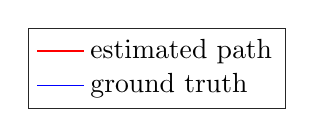
\begin{tikzpicture}

\begin{axis}[%
width=0.951\figurewidth,
height=\figureheight,
at={(0\figurewidth,0\figureheight)},
scale only axis,
xmin=-279.909634132857,
xmax=368.981031803275,
ymin=-17.60491,
ymax=494.181437810917,
axis background/.style={fill=white},
legend style={legend cell align=left, align=left, draw=white!15!black}
]
\addplot [color=red, forget plot]
  table[row sep=crcr]{%
-0.0254918464850879	1.53029535298812\\
-0.0249375910222026	1.94734709129116\\
-0.0603236978857134	2.6546735108884\\
-0.0898810439677802	3.26129873758476\\
-0.122075910018214	3.77863002775995\\
-0.159570842980351	5.84214038823406\\
-0.162924757869628	7.08369056436346\\
-0.345776789656578	7.86663308840249\\
-0.274915939891177	8.64211113562301\\
-0.309598017917685	9.85377995390351\\
-0.277110670012233	10.8074353831107\\
-0.341823185024733	11.5749687633776\\
-0.217611982003351	12.8917266019904\\
-0.0592982609196149	14.535514156623\\
-0.180911942853752	15.86511539354\\
-0.677175153351174	16.7429228811065\\
-1.42757029229411	18.598720661044\\
-1.26066526013012	19.5585825630115\\
-2.09099544665857	21.9137054411806\\
-1.35489091310912	21.6821311104135\\
-2.27343895842534	22.8531216527086\\
-1.72365781744713	23.8629426632053\\
-2.38412979098817	23.3141018626733\\
-2.49982652481565	23.8960769977063\\
-2.64934504463407	25.1017570623487\\
-3.24102646673798	26.8294184308591\\
-2.75227337081859	26.1588342526725\\
-2.25251316649116	26.8675605071435\\
-2.23514914963694	27.9032151877208\\
-2.24609116891217	27.982958602682\\
-2.30118561315577	29.7433987882563\\
-3.41100800227531	31.3865178280425\\
-2.87855773515937	31.9140170643668\\
-3.4368663602838	32.4538719579672\\
-3.11388619330194	33.5688756020074\\
-3.78881356739435	34.4364391121824\\
-4.14043694611709	35.5639350903059\\
-4.24265980636678	36.3360170131273\\
-3.08199500842777	36.2823617856426\\
-3.86218254810391	37.5247117612819\\
-3.78008871169758	38.4796755619529\\
-3.83925339983511	38.9776212507811\\
-3.62251987051958	40.2651303460199\\
-3.72476804662364	40.9917500495216\\
-3.87491538823995	42.1588347214711\\
-4.05345949138225	42.9264327799661\\
-4.55990685408857	43.7076616826611\\
-4.58710434912859	45.1266030356705\\
-4.15662131379484	44.9102241274385\\
-4.32432900127588	46.2011578203503\\
-4.42985739443779	47.0656224658856\\
-4.42962961862714	47.6679605163711\\
-4.57070652957851	48.2221793741606\\
-4.57199673235862	49.4317077831228\\
-4.29788818939738	49.9869788210274\\
-4.3021976565471	50.6767884176887\\
-4.25836254668855	51.4045082969207\\
-3.97410735341543	52.1564613562996\\
-3.52845109049775	52.8879090013884\\
-3.60817948812444	53.2910941672489\\
-4.21767101402003	53.3037102904217\\
-4.26694066421515	53.8252814238761\\
-4.11785254389759	54.1293280041667\\
-4.15707496458134	54.5577610053573\\
-4.41885416695881	54.8395840597333\\
-4.47213079181435	55.2228225873175\\
-4.52586244161301	55.5628903543122\\
-4.66934918726159	55.9017966549809\\
-5.01078860658352	56.2552944315139\\
-4.99428493090294	56.7287729123666\\
-5.02572974611267	57.2588695056402\\
-5.37562191299367	57.7729895574645\\
-5.55237267108766	58.2709251365913\\
-5.44156048501393	58.5639284681207\\
-5.51439869195852	58.9648517597728\\
-5.41642527121364	59.1741555806045\\
-5.60175869371574	59.6963392380832\\
-5.52621049213029	60.0824383205396\\
-5.56512749107208	60.3373151897335\\
-5.65385745413775	60.5368668895362\\
-5.68238964306415	60.7028096755688\\
-5.8506642780277	61.246073230544\\
-5.86068903911556	61.5261630823309\\
-6.0071631450362	61.8201105758982\\
-6.05463522152146	62.2264536916792\\
-6.18359650084802	62.5925169496036\\
-6.16567179398064	62.7721368567187\\
-6.21525354541593	62.9316117983634\\
-6.3728097185946	63.4879041554613\\
-6.3431659748768	63.4859762083145\\
-6.35139809038352	63.6602334297999\\
-6.38096676618425	63.862338851775\\
-6.60340421631325	64.1617853723935\\
-6.47215441417714	64.0923429649715\\
-6.55668332626107	64.3099106129619\\
-6.49413587102935	64.2257225029357\\
-6.48736269570742	64.4231285975602\\
-6.44410730694348	64.5107297521112\\
-6.44742249079286	64.5523797638164\\
-6.46112710882803	64.7596513816304\\
-6.56943486128485	64.9974825541328\\
-5.16228308479518	66.3556355531066\\
-4.73470261263065	66.7887889519573\\
-4.15030439116621	67.4261352053223\\
-3.86240211844175	67.7385412514972\\
-3.44978892931622	68.1035016089998\\
-3.13110621496826	68.1794287485119\\
-2.70805200334046	68.7266136838131\\
-2.7484777951657	68.7613365329827\\
-2.67402025313584	68.7014394323924\\
-2.92527792771013	68.7445552141848\\
-2.7694337810359	68.7533953308252\\
-2.79048689029027	68.7613319033532\\
-2.71623548387942	68.7531223981402\\
-2.64937978216835	68.7662189471711\\
-2.5697465082081	68.7592746391713\\
-2.49264984133266	68.762684434947\\
-2.56442326584954	68.8028874257184\\
-2.42108497972657	68.7452612745006\\
-2.39158148285952	68.7352580976468\\
-2.36767408897901	68.7549506392439\\
-2.31854867713639	68.737357878982\\
-2.25326308040345	68.8030997415243\\
-2.24790489017158	68.8047366095008\\
-2.20922982360595	68.7617953212112\\
-2.11456252891895	68.7041110052127\\
-2.07794541546117	68.7167137088228\\
-2.04011602038262	68.729996900092\\
-1.96444366262119	68.7198340391341\\
-1.90756392847745	68.7372041142033\\
-1.82818010808397	68.7446402253316\\
-1.76544743007254	68.6997819991224\\
-1.69921521961514	68.6844677704676\\
-1.58205436235882	68.6656632810822\\
-1.49136216772553	68.6831456520077\\
-1.4567101931077	68.6608012706501\\
-1.37374816690968	68.633288570018\\
-1.28426654003647	68.6327384078201\\
-1.24221808889874	68.6359465034188\\
-1.1392430160249	68.6203531059414\\
-1.07838210175362	68.6022228751043\\
-1.02353544843056	68.59479665955\\
-0.981007408538902	68.5528204582562\\
-0.880835988977299	68.5492523221916\\
-0.773450073505957	68.5618566392044\\
-0.695800854404705	68.553673402724\\
-0.601504810136044	68.5324317021409\\
-0.466262010668162	68.5166525796782\\
-0.4343579768875	68.493617385709\\
-0.27599634333942	68.5390424448537\\
-0.206137094976174	68.5193363033419\\
-0.166468808423057	68.4977587592106\\
-0.111206330219467	68.4914264680322\\
-0.0417599751618329	68.4921024462819\\
0.0145967346588751	68.4905771615433\\
0.0789563129061079	68.4706575793494\\
0.15111278071101	68.4613257380359\\
0.200445783954544	68.4593257460154\\
0.242432348854578	68.4563843348551\\
0.290143802472025	68.4307018493228\\
0.411268236790518	68.4136438973036\\
0.457033835052604	68.3989872633654\\
0.515167331974428	68.3994790841074\\
0.55311643027307	68.4048832502122\\
0.622834119560803	68.3494574511098\\
0.679235281916124	68.3588114114493\\
0.738647338838874	68.3309205932311\\
0.799304002357957	68.323633803502\\
0.844364545325067	68.319070801932\\
0.874365080037666	68.3206835522439\\
0.92085338499497	68.3050094858578\\
0.970626824519204	68.2933698243747\\
0.994206882684974	68.2800649155739\\
1.06698793905533	68.2668155044703\\
1.12788144409291	68.2437384960775\\
1.19320101142402	68.2319400046377\\
1.17257414431613	68.2258334498327\\
1.22329853867889	68.2110008016179\\
1.24790518322945	68.2001419758047\\
1.28356747582186	68.192860423682\\
1.31970516379937	68.1868566172963\\
1.36855540633614	68.1641922096217\\
1.40072314791968	68.1677282037599\\
1.42956937777001	68.153340480122\\
1.45903301850508	68.1408743154444\\
1.49339510467069	68.1379865518586\\
1.51897631056026	68.133565552244\\
1.54227867288268	68.1319171760544\\
1.59198775263162	68.1274163299167\\
1.61606520743447	68.1245428558043\\
1.64233479578505	68.1243320091555\\
1.67524473461454	68.127474122683\\
1.68890821678942	68.1350127553357\\
1.72532119481408	68.1397308637361\\
1.76040497393434	68.1360895465111\\
2.32637912813648	68.7409965881226\\
2.42557657927692	69.4356487795147\\
2.82984745136007	70.5187103630926\\
4.25243057380952	72.0532863930487\\
4.743631161746	72.7216964925602\\
5.11167469345136	73.3125483069339\\
5.6350054107305	74.231019644157\\
5.89503172952666	74.9362052459969\\
6.32225285236306	76.1189971093224\\
6.7572360405468	76.8696659392275\\
6.90739320692241	77.5698244255377\\
7.49263682144471	78.3555015313727\\
7.84297805349701	80.1064069924676\\
7.99335238523177	80.7065246483307\\
8.39759306420759	81.5202349475433\\
8.65915222013725	81.9493397902011\\
9.16500848676621	83.1967996532794\\
9.45629116759457	83.9375969381233\\
9.63593950681243	85.4815585382871\\
9.88566503644274	85.6315093336213\\
10.2428159132173	86.1265775074272\\
10.7343170245853	87.0828301227972\\
11.0683508107053	87.8736550768478\\
11.1944395496445	88.8970682204383\\
11.4530532318159	89.520605401569\\
11.8186901035052	90.4342172333372\\
12.2614853153901	91.3751535308857\\
12.3749594962316	91.8626890835962\\
12.5739822808096	92.4543697583223\\
12.8979899167476	93.129736020434\\
13.2326878381812	94.4439277313354\\
13.4058288239662	94.5877643227907\\
13.661653488144	95.0940348617212\\
13.903690359268	96.2475913586399\\
14.2988108459682	97.1008676425508\\
14.6077945077504	97.4976415288364\\
14.8958426079441	98.2950626150742\\
15.0074391447246	99.4179952185034\\
15.5491287445354	100.056500746182\\
15.760645617501	100.705357848524\\
16.0128707430768	101.611758095886\\
16.4209885819264	102.656763647934\\
16.7064441880337	103.624969763649\\
16.8700416719813	104.195489666811\\
17.3323404016183	105.746842606074\\
17.1500845522763	104.796547838137\\
17.7342153984745	106.109213751717\\
17.947443290581	106.886431030478\\
18.2432701562009	107.211416478416\\
18.4334315273966	107.397685034675\\
18.492104524037	107.43590895294\\
18.5994569104962	107.43266513871\\
18.9436247371266	108.887253352146\\
19.3043004507618	109.930134967356\\
19.6159352129066	110.296514961295\\
19.9441223687576	110.992038667573\\
20.1482910090224	111.814340931271\\
20.5598264302592	112.083029189193\\
20.9163956134198	113.759018685618\\
21.693339699139	113.787759185057\\
22.1847793331632	115.329250169106\\
22.6089748572092	115.242261070234\\
23.0434764814109	116.589954563773\\
23.6422337305103	117.155429084836\\
23.8547573033722	117.028726449226\\
24.4331179092936	118.199672954091\\
24.9351621109058	118.617531584534\\
25.6625666605772	119.882636912585\\
25.862259517254	120.882595670922\\
26.4710335079412	121.631973416107\\
26.8790165665103	122.068906674435\\
27.6078895609699	123.301606328221\\
27.7610706813634	124.19110486594\\
28.2690748048773	125.090545442458\\
28.9278280044138	125.634671588503\\
29.6680272897553	126.159756389979\\
29.916775241472	126.881179974329\\
30.5104544839036	127.785982831923\\
30.9864693764466	130.070526437571\\
30.8935350423897	131.129137670745\\
31.0059332179696	132.201935583778\\
31.1228205698849	133.52437635679\\
31.3466746411097	134.408331037195\\
31.4038472420089	135.544180746494\\
31.3692358417206	136.681231107119\\
31.5231719314328	138.079832590986\\
31.336375125949	138.355879466341\\
31.4807096726588	139.589486598582\\
31.2574926224906	140.225275633466\\
31.6521669792042	140.932496301322\\
31.4446320210861	141.627832908823\\
31.5284292216924	142.368589669191\\
31.5046296987031	143.305498379961\\
31.8523224522124	144.224733848999\\
31.4315420575404	145.012784307816\\
31.4005452744225	145.761996403217\\
31.3806275046288	146.38775916824\\
31.3225631868471	147.389483403713\\
31.5092562119486	147.925791555093\\
31.5641072238436	148.789220058573\\
31.8288072822233	149.536428548023\\
31.6219988108419	150.314959768323\\
31.6281419965141	151.19917329465\\
31.4316332777911	151.918602352687\\
31.2275407321085	152.58379355785\\
31.2873535146033	153.347962871355\\
31.226682329582	155.211645077753\\
31.2306630352108	156.174631377729\\
30.9564003832906	156.516056708928\\
30.7626843788353	157.385496929875\\
30.8728564574075	158.385369751966\\
30.7663971874074	159.045498570815\\
30.8580800859372	159.841535501677\\
30.7747174099569	160.650241483534\\
30.4952422119895	161.312021792366\\
30.3131850401837	162.263656850787\\
30.1740873299001	162.988327106877\\
29.9877537284804	164.000282832893\\
29.770116234785	165.019585765822\\
29.4097950429042	165.653169318273\\
29.2606187292257	166.544578567415\\
29.1530661213472	167.764357603646\\
29.0036085385588	168.901269796661\\
28.9249761117594	169.998121344367\\
29.0305034055131	170.887919160539\\
29.1108749051132	171.683336623426\\
28.8488903953836	172.583733460536\\
28.8592534591764	173.582579960207\\
28.7564515170669	173.595521113834\\
28.6339041355323	174.307634711422\\
28.5071186672631	175.485720421626\\
28.3739764649885	175.613968442466\\
28.4258538529184	176.407227632034\\
27.8055077526936	178.182678071383\\
27.6028273177362	180.071426595132\\
27.6706284214983	181.393143065044\\
27.5714094736419	182.378457465733\\
27.3345962035589	184.297725437826\\
27.2050946893493	184.852792513314\\
27.0273970903181	185.80953423445\\
27.0696777142104	186.367454987379\\
26.8790358027877	187.070788115954\\
26.835616545771	187.872250955736\\
26.6688072627824	188.479385263934\\
26.451423500193	189.103604111808\\
26.2099976579884	190.008257479677\\
25.8936463365625	190.723665157023\\
26.0214872958566	191.41048176177\\
25.9223815739118	192.072325809546\\
25.8885468322707	192.556858431119\\
25.655178520461	193.488491817572\\
25.6041712223397	194.096876321591\\
25.5542120919866	194.859843310874\\
25.6147810425441	195.267942561724\\
25.7964288253991	195.616738472469\\
25.634793202666	196.427482122492\\
25.8194364080329	196.669795839361\\
25.6930298943844	196.934463548948\\
25.8560220238842	197.586265492008\\
25.7443452290368	197.880702781958\\
25.7050015472644	198.162392567377\\
25.45264865354	198.916789034969\\
25.5216566400808	199.47729416911\\
25.39486818651	199.8917475016\\
25.3823838189762	200.430621275378\\
25.3918465236732	200.805200354695\\
25.3714867622897	201.125521219416\\
25.336604991804	201.759935573005\\
25.2412254219563	201.776461977076\\
25.2283632089339	202.028639766291\\
25.1993337604282	202.26625898985\\
25.2115271331007	202.544861450753\\
25.2127826740648	202.820300479003\\
25.1417397075799	203.120935105433\\
25.1286994092587	203.34223235254\\
25.1608137399525	203.63104704152\\
24.8645712183388	203.961310126502\\
24.7865644352517	204.346462328168\\
24.7695377621816	204.667691677212\\
24.8122071734759	204.929472113458\\
24.7344360646849	205.356025866679\\
24.7313817895402	205.545961284727\\
24.6216376080747	205.919818508193\\
24.5361418913689	206.285323902868\\
24.5262873359962	206.619266792245\\
24.4280411379531	206.93297503833\\
24.4868197675078	207.23352721783\\
24.3620964141778	207.532373922107\\
24.3443266644148	207.923351840319\\
24.2899831134889	208.302867722769\\
24.2056541730923	208.620881532893\\
24.2671794104946	208.830538705943\\
24.2256210632622	209.097985126339\\
24.1635833921456	209.431120865591\\
24.2233287801773	209.753566667915\\
24.2245059323107	209.975924755926\\
24.2773876722535	210.0280206528\\
24.2153841830566	210.339243146341\\
24.1471369166393	210.554585854975\\
24.123640650444	210.808817936811\\
24.0231940665651	211.092799675821\\
23.9991855615781	211.255022307387\\
24.296872806854	211.092929051617\\
23.9822441068207	211.527249206175\\
23.9663092023658	211.509639175926\\
23.9846432853858	211.347632540596\\
24.0325470142418	211.349196736734\\
24.0407842533872	211.356997105029\\
24.0190527441633	211.210934216378\\
23.777087003753	211.686636966901\\
23.6290913503958	211.754922423789\\
23.347617750422	211.315916522719\\
22.2524627030443	211.293173409533\\
21.73124023025	211.621101209519\\
22.2464970002914	212.042059997957\\
22.7313425290074	212.08134723709\\
23.0354084648533	212.123513276966\\
21.4134480282015	212.589471750404\\
19.7979307066517	212.913217797488\\
19.2582905686774	212.884911382348\\
19.1678545763804	212.647773213406\\
18.2483010946474	213.308255642926\\
18.1497635544864	213.482520091896\\
17.5661112332419	213.846523682728\\
16.6291258037731	214.27415240985\\
15.4157968044397	214.186375980845\\
15.3663427688224	214.233570425831\\
14.9142040393703	214.076332603915\\
14.5382827027154	214.013088263563\\
13.4904734289621	214.626781031759\\
13.0930353529109	214.357473836844\\
12.1321476337684	215.038762249081\\
12.0048455141304	214.479461964732\\
11.5166877275124	214.343992242921\\
11.2594441579004	214.365571889851\\
10.875476560048	214.586743906002\\
10.5620231890785	214.345061005698\\
9.67465674002987	214.495829507906\\
9.29944832590777	214.554881514925\\
8.80139367164341	214.798070626697\\
8.08093368817823	214.857404698567\\
7.55624547608903	215.125308174891\\
7.33934871340871	214.867432865852\\
6.81292613526508	214.712556664222\\
6.23647880029449	214.854215357086\\
5.93709101155725	214.638949301433\\
5.11450982724467	214.83853329361\\
4.53934808805743	214.796327079969\\
4.10356983637135	214.930740172533\\
3.54342325576398	214.750326372446\\
2.91900538966626	214.855105243567\\
1.92114104206102	215.036547880958\\
1.83017110963159	214.844064685131\\
1.13166415742217	214.991768665409\\
0.795647525566089	214.914248164717\\
0.423140774757908	214.864776410601\\
0.589737107243323	214.769381925329\\
0.393611465711487	214.691793442922\\
-0.319356415268118	214.869781348428\\
-0.395886850728132	214.679808906286\\
-0.926122499699243	214.722523351686\\
-1.07053173999774	214.666469876697\\
-1.267531205691	214.605705001317\\
-1.59833670719756	214.555592137776\\
-2.18928151947033	214.669281051706\\
-2.45883827287967	214.657249576627\\
-2.61299595524665	214.593288620563\\
-3.10517987313153	214.722375792856\\
-3.32237209041765	214.63695728217\\
-3.61088863411375	214.569154220346\\
-3.79532226882941	214.538822254458\\
-4.10453752687978	214.512243612151\\
-4.51906713964134	214.447003648654\\
-4.77442366364141	214.422729982806\\
-5.13341990484228	214.424987260822\\
-5.33751944152229	214.304420156075\\
-5.69933848586392	214.310484343659\\
-5.82938422985549	214.205648373489\\
-5.97607562187358	214.23161507837\\
-6.08421126276354	214.141095761368\\
-6.19156477763469	214.148061810589\\
-6.35516108177956	214.027083039427\\
-6.79278687489574	214.158843240963\\
-8.88470477438872	214.00388554744\\
-9.5602040296985	213.497422675691\\
-10.3436532243474	213.573031472916\\
-11.2414652349485	213.462680855285\\
-12.047769715407	213.156959254144\\
-13.2342075482977	213.225157546666\\
-14.3577549505562	213.210457570065\\
-15.2708107054786	213.144543970133\\
-15.7291004810213	213.034415470773\\
-16.704549727583	212.951822592387\\
-17.3808564994151	212.637022189031\\
-18.7991388507424	212.966865047599\\
-19.0953427731673	212.861572662411\\
-19.3619714962359	212.479895910625\\
-19.9376331202177	212.416179263601\\
-20.4622915085327	212.382166887641\\
-21.2685842433885	212.277015414084\\
-22.1354251151204	212.434877366505\\
-22.7481600732877	212.597266370167\\
-23.7113121286454	212.809241576281\\
-24.572830829869	212.474581741946\\
-25.0057571871728	212.618232136984\\
-25.7452986609307	212.618093541893\\
-26.4145191978103	212.66790332991\\
-26.7471187596246	212.721332620844\\
-27.5497642389168	212.883190508485\\
-28.0450254576246	212.815482437103\\
-28.4263283425603	212.856750314121\\
-28.8520835568439	212.837988969263\\
-29.2247156330257	212.689012106691\\
-29.7583753912387	212.904208868114\\
-30.2091977104723	212.815413466712\\
-30.5946019859669	212.908389382693\\
-30.8303034923719	212.92234164273\\
-31.1790803695378	212.820781076697\\
-31.4784184690701	212.904773760019\\
-31.4049760659972	212.934092025406\\
-31.6080873367598	212.935297227569\\
-31.7384907553753	212.851716191155\\
-31.8898459052867	212.818220024182\\
-31.9638974764624	212.829094001591\\
-32.1824879928357	212.98841687425\\
-32.1655223170709	212.840021572307\\
-32.1923908149378	212.9172267565\\
-32.0916810749162	212.91030020718\\
-32.1489909083316	212.896514607043\\
-32.15964305121	212.942742021821\\
-32.2000980408644	212.904409072289\\
-32.1926832969525	212.914999300785\\
-32.1489311833243	212.928029674289\\
-32.1417631721691	212.929110146895\\
-32.1752900774627	212.941440586801\\
-32.1215717355744	212.923694104363\\
-32.2254422252891	212.898680008697\\
-32.099820638685	212.918205505977\\
-32.3012840382865	212.849441959141\\
-32.2401240422764	212.892675756026\\
-32.1059648103308	212.898156761293\\
-32.2187080066856	212.857117284202\\
-32.2849660052344	212.91479898346\\
-32.3053575615531	212.896996909545\\
-32.3908949545142	212.916195285458\\
-32.3691386656538	212.913586729109\\
-32.4840201353643	212.862941086131\\
-32.6233134103869	212.858265977824\\
-32.7068969515437	212.888763395313\\
-33.2174837373732	212.945253061197\\
-33.4373042866178	212.80362060497\\
-33.5662675146952	212.854121105593\\
-33.918576969566	212.956682674868\\
-34.1750611501107	212.900609851177\\
-34.3050970169915	212.980494311042\\
-34.7591335306888	213.230402599525\\
-35.0133240475871	213.110161487189\\
-35.1027949518492	213.062289142315\\
-35.3856731622133	213.273421391619\\
-35.4886092932079	213.301003918611\\
-35.9353010442333	213.344452939839\\
-36.0205759616671	213.552351596785\\
-36.4321499581096	213.6355438708\\
-36.6630331594686	213.698629205214\\
-37.4571198298805	213.987346099098\\
-37.5561187478809	214.18551884902\\
-38.030548384609	214.461430410488\\
-38.2360149590335	214.659015176915\\
-38.7131687933331	214.886831225974\\
-39.2365113985385	215.257630458455\\
-39.4370799656358	215.689444867075\\
-39.5503623257288	216.027016510892\\
-39.7905470537138	216.326888932857\\
-40.252653846781	216.84613291881\\
-40.3111508848086	217.432588396869\\
-40.6156984536395	217.744486044755\\
-40.8473865542094	218.319065934572\\
-41.0893217248059	218.674494817595\\
-41.0774102378002	218.742966840269\\
-41.5222631015515	219.802071979507\\
-41.7411348174162	220.217207900609\\
-42.2345021377749	220.998391819105\\
-42.5176819356347	221.431961240657\\
-42.8592816956743	221.827565468201\\
-43.5110475720288	222.853237577047\\
-43.9224051734094	223.83577780191\\
-44.0229368417564	224.787218372985\\
-44.3259876952366	225.739007947086\\
-44.2861194606393	226.237304108418\\
-44.6137712157757	226.237631739993\\
-44.7091554419576	226.576856364125\\
-44.7116951785624	227.287873256857\\
-44.8423914174883	227.625587539739\\
-44.6970852206428	228.047112811744\\
-44.7059763403861	228.228507053352\\
-44.8908655809168	228.910411746398\\
-44.9740871271561	229.374442034491\\
-45.1344783697858	229.934920204791\\
-45.2212898538476	230.417483410399\\
-45.3790843504595	230.928079585211\\
-45.4206004797457	231.224953745021\\
-45.4308381858286	231.736006403963\\
-45.3300060452855	231.700480568538\\
-45.7891901579862	232.251789804872\\
-45.84726280253	232.607707089245\\
-45.9257479418923	232.874296094355\\
-46.0917299313781	233.636686653868\\
-46.2203703593597	234.247682205506\\
-46.3094706964418	234.683288644602\\
-46.4473023338355	234.973072461477\\
-46.5603347315074	235.262463892118\\
-46.6431314821818	235.719033916002\\
-46.7226948076352	236.113304962719\\
-46.8161031493154	236.445965880473\\
-46.9075886961262	236.672789912754\\
-47.081739943149	237.488090828786\\
-47.2010674183691	237.809628867081\\
-47.246512765219	238.505143654282\\
-47.1473131458185	240.441319121648\\
-47.2324589011008	241.361301522648\\
-47.422539945568	242.086540900497\\
-47.1548958910591	243.341582853407\\
-47.1247005117633	243.989390924863\\
-47.0963491584297	244.828805920311\\
-47.0224336947515	245.626737679853\\
-47.0501833043112	246.700490314079\\
-46.9542678656876	247.346715397458\\
-46.8739159753082	247.977698935206\\
-47.3139505715168	248.514304708373\\
-47.5031451145017	249.383264734853\\
-47.6894072119365	249.605704301269\\
-47.9822090892648	250.326250440796\\
-48.1930909511224	251.381780851603\\
-47.683497608932	253.346961566476\\
-47.1437025965653	255.269188919135\\
-46.9555399297772	255.728788855105\\
-46.9113871215947	257.540988819626\\
-46.4018998531305	258.215020825359\\
-46.1691399624514	259.169708499103\\
-46.0006329777693	260.144908009681\\
-45.4942496213327	260.861282448583\\
-45.1837996456915	261.695799310811\\
-44.8439308560947	262.945669476523\\
-45.031056448566	263.445196847028\\
-44.6051055468825	264.644878476725\\
-44.5375296457634	265.52298933947\\
-43.9379023975452	266.734832466098\\
-43.7761271905091	267.611227603413\\
-43.2437162313124	268.112421714943\\
-43.3574505322155	269.036962788332\\
-42.8119051592064	269.969030602106\\
-42.6380071422129	270.653681792449\\
-42.8539840160955	271.25007885561\\
-42.430597124949	272.125926734298\\
-42.1451730155138	273.102027691711\\
-41.8563532834494	274.087495671695\\
-41.2968953440232	274.936185282528\\
-41.2225874507555	275.917660109676\\
-40.8923722906232	276.749409408474\\
-40.6038548602881	277.849571215356\\
-40.1537628651525	278.480987491248\\
-39.8130405265665	279.481478060277\\
-39.4631222518126	280.37412522484\\
-39.0252560389229	281.084480035055\\
-38.2881664842881	282.380661662572\\
-37.8950494319854	283.199695717622\\
-37.4156696292089	285.377285892079\\
-37.1246989925732	286.567755242813\\
-37.0078289946857	287.759353528826\\
-36.4235674532139	288.655128827211\\
-36.4206719222769	289.479169194261\\
-36.0199877742188	291.388416932704\\
-35.7371574949692	292.287462651489\\
-35.4944568807212	293.428513242332\\
-35.0724434707039	295.326881637912\\
-34.9267090809202	296.357985976457\\
-34.7962987803007	297.304945783259\\
-34.6677445856661	298.406750037939\\
-34.4175366530386	299.203530674089\\
-34.2497002644438	300.050480234458\\
-34.025015461553	300.846638483316\\
-33.9052652051478	302.057645773539\\
-33.8262493158549	302.886600286682\\
-33.5523434137671	303.928982136653\\
-33.0947880894399	304.839200182004\\
-33.435879549583	305.517276228189\\
-33.0356890527176	306.281694684402\\
-32.9853019988319	307.248799760557\\
-32.9544689753232	307.927088377347\\
-32.220810070766	309.150152962646\\
-32.1525551845704	309.759636242243\\
-32.9989570805084	309.915338106239\\
-33.4321504999133	310.186200619098\\
-32.9836081768361	310.905274657959\\
-32.5750584820784	311.665455473466\\
-32.0190359696176	312.814504882672\\
-31.4700124082084	313.798267948704\\
-31.0882394843671	314.232613800771\\
-32.6048323084808	314.979950582979\\
-30.4822555189457	315.811317736442\\
-31.0292626567009	316.382484300536\\
-30.9310114462225	316.87814082286\\
-30.6864767041683	317.886727392411\\
-30.7726610461201	318.993196905374\\
-29.0576603098639	319.798787959842\\
-28.7711605010995	320.623311392259\\
-28.7093404830653	321.259517703079\\
-28.9041161327918	321.972302837225\\
-29.0941573601318	322.771694921716\\
-29.0994113613896	323.675771526195\\
-29.0885143088973	323.429907778961\\
-29.3428586520038	323.795665938011\\
-30.0541236364524	324.06992945094\\
-30.0695284081772	324.524674301971\\
-30.0250587285471	323.99094762543\\
-30.0815687814954	324.407852889984\\
-30.2664215409223	325.061368068208\\
-30.5387720312818	324.548372508383\\
-29.8153167473754	324.460218777784\\
-30.2202994195	324.812651250332\\
-29.9255936919935	324.4731767891\\
-30.2564989140735	324.809243384898\\
-30.2160583559844	325.045066532158\\
-31.9520686894934	326.035155722726\\
-32.6222818170176	326.559188293965\\
-33.2138329306937	326.536234127881\\
-34.7489286227544	327.291839472857\\
-35.8494644332291	327.531403381621\\
-37.083633031998	328.035070118398\\
-38.6536244031342	328.859228715703\\
-39.4408761340687	328.729092545352\\
-40.6655524623809	329.318066798766\\
-42.1020469335577	329.677156840239\\
-44.2040416163879	329.612365954592\\
-45.6794767154268	329.868795854747\\
-46.7064011268461	329.546411286154\\
-48.614928246103	329.378190940468\\
-49.9309875262262	329.635189708725\\
-51.3563823558072	329.723357193928\\
-51.0978106620835	329.908610425922\\
-52.2001043527608	329.790119639989\\
-53.877185604255	329.556497371619\\
-55.036841966622	329.621806594873\\
-56.495076964268	329.946714257879\\
-58.0801408344746	330.254718163287\\
-60.059959450994	330.300764588298\\
-61.2911627109869	330.101095233726\\
-61.8985535743654	330.214282061376\\
-63.0434713996976	330.21308547089\\
-64.5674860363518	330.209961250284\\
-64.571133956562	330.349796581707\\
-66.252740907551	330.426465380046\\
-67.3101021438173	330.507246990496\\
-69.3443083489517	330.711530451238\\
-70.4757133828234	330.589493937085\\
-71.6656722855487	330.544071468239\\
-72.4464422085937	330.784337440676\\
-74.3395275300129	330.883615340343\\
-75.3250730270993	330.95899134696\\
-75.9760534680185	330.949121200304\\
-77.4039667771099	330.826729931524\\
-77.9830187850089	331.000247864272\\
-78.8687689456271	330.936635887811\\
-80.2344578369083	331.277002425432\\
-81.4185828783275	331.180546591004\\
-82.1579831466836	331.255430568315\\
-84.2701165695666	331.331188785134\\
-85.381765018527	331.328927260221\\
-85.9187303825449	331.342604183633\\
-86.0058085659101	331.596210159356\\
-86.6345463070181	331.704106100662\\
-87.1532675488185	331.573066087587\\
-87.8758778539771	331.949890100947\\
-88.5495553098208	332.12871940584\\
-89.0586796220371	332.069320924164\\
-89.395828767759	332.256034299604\\
-90.3906163926342	332.250450270316\\
-90.6364606915531	332.613369771351\\
-91.2923595527582	332.826427360494\\
-91.6158289510457	332.932953700456\\
-92.3925204689356	332.926229695809\\
-92.6201219071659	333.050243107929\\
-93.6608464832948	333.26887947839\\
-94.4564065706272	333.391609558434\\
-94.9726830240708	333.31261823923\\
-95.3938220813347	333.471138520326\\
-96.0267459745488	333.776066349316\\
-96.4667262182685	334.09191598723\\
-96.8006882772589	334.344229082932\\
-97.7038509323724	334.315042074222\\
-98.2508769633903	334.332510376898\\
-98.4998469680749	334.608676587533\\
-99.0010742313726	334.460400574565\\
-99.3772112309244	334.87542186045\\
-99.8433775263427	334.969477408754\\
-100.369196958569	334.816270984674\\
-100.649054809036	335.144544991477\\
-100.884502098649	335.11477631906\\
-101.399073744781	335.147006853795\\
-101.655398223972	335.214153157286\\
-101.943192743224	335.139046799433\\
-102.246850048485	335.400610178079\\
-102.490391100558	335.302013711441\\
-102.959386146335	335.335032828147\\
-103.235184130284	335.159673109969\\
-103.533272683701	335.167071109366\\
-103.787873027846	335.10828616072\\
-104.177976753419	335.076443599708\\
-104.442229917373	334.932458772789\\
-104.69957459767	334.820706066122\\
-104.95390297583	334.646222726798\\
-105.442052158665	334.784885639064\\
-105.523430740352	334.648393119687\\
-106.162055256026	334.685078637888\\
-106.419529930642	334.73982636409\\
-106.740111361581	334.679535636641\\
-107.013001576927	334.527776532129\\
-107.29244961418	334.487849615371\\
-107.717829637576	334.354699620496\\
-108.015942696537	334.306738033252\\
-107.973778380001	333.982257556483\\
-108.400981083681	334.04631437748\\
-108.877448657914	334.029644085789\\
-109.67857339769	334.185142370678\\
-110.116884349427	334.087659682204\\
-111.90624992421	333.515256346859\\
-112.879919763106	333.268432338534\\
-113.733477980254	333.152697204073\\
-114.477870675761	333.280187897946\\
-115.134794276	333.362493838527\\
-116.29925573759	333.279273206963\\
-116.592195632737	333.099436641115\\
-117.4469544453	333.255064924585\\
-118.311459427027	333.266768218191\\
-119.142995658145	333.386375393761\\
-119.5519804159	333.143294097204\\
-120.125727095054	333.229007628851\\
-120.599301493847	332.917557923802\\
-121.41050654491	332.941315350844\\
-122.010740708945	332.683071914598\\
-122.448065444772	332.740223493192\\
-122.737659238848	332.506115198567\\
-123.319242686169	332.37173759706\\
-123.987170959506	332.216396772916\\
-124.699999564765	332.094822017949\\
-125.300055595285	332.14542450167\\
-125.832855582729	331.940284959672\\
-126.279710584852	331.882406939749\\
-127.204212105544	331.740714442927\\
-127.437097449713	331.582905914604\\
-128.047247777049	331.428515154805\\
-129.876237550654	330.829171331589\\
-130.675736570094	330.567752334914\\
-131.570550603339	330.320907279621\\
-132.496049348151	330.14786487886\\
-133.884600251746	330.225623704696\\
-135.147411479847	330.029604868238\\
-136.572718042015	329.845383755894\\
-137.396388652978	329.775610094747\\
-137.918188575155	329.630338461391\\
-138.941678383965	329.541154961344\\
-139.627816168456	329.505438319312\\
-140.279651442428	329.345139677669\\
-141.792467729002	328.383745769038\\
-142.483116797835	328.030731515725\\
-143.797691730101	327.331695780086\\
-144.652175696273	327.009717122671\\
-145.173094563113	326.707886081164\\
-145.460328039472	326.441495551787\\
-146.246866769475	326.146609899088\\
-146.668040309708	326.000219841559\\
-147.321275893584	325.777797065317\\
-147.683129388003	325.488427994554\\
-148.195929444065	325.364505374244\\
-148.365987947546	325.059133930781\\
-148.826378158346	324.919332220775\\
-149.467056581452	324.542590690758\\
-149.761458285886	324.45875226042\\
-150.238774904033	324.208785529118\\
-150.65551674814	323.969433938326\\
-151.12117195531	323.723785882836\\
-151.438736664022	323.540682132909\\
-151.964496223281	323.240518656497\\
-152.316078225546	323.020792357025\\
-153.04437643066	322.859905288161\\
-154.031536232429	322.709983758657\\
-153.972702827433	322.666683382184\\
-154.829604253641	322.337053066111\\
-155.390334144188	322.166804669758\\
-155.880416335035	321.984899150535\\
-156.193162072909	321.739684416764\\
-156.434391946001	321.838273864625\\
-156.515287540772	321.654037114348\\
-157.010276722406	321.527434897005\\
-157.244448124897	321.48013903531\\
-157.921143964233	321.283412530287\\
-157.861556455003	321.263850761104\\
-158.130419362393	321.124020948531\\
-158.131966355271	321.159737586622\\
-158.548488606006	321.015362563419\\
-158.657462295401	320.880857157309\\
-158.825540420148	320.732333686745\\
-158.955732436493	320.628360019961\\
-159.178561595351	320.545081654653\\
-159.137506761558	320.408073940571\\
-159.281509093168	320.269489058068\\
-159.317908848195	320.210843154201\\
-160.478123333959	318.682124414268\\
-161.139149377988	317.936759801109\\
-161.762842249052	317.164990636701\\
-162.110243690989	316.516665543159\\
-162.52246555518	315.78798297121\\
-163.062406545729	314.959480615909\\
-163.36841871443	314.069741823325\\
-163.84157453904	312.945700811698\\
-164.125975728303	312.071284641597\\
-164.140790938608	311.083827897955\\
-164.279777171775	309.839777746885\\
-164.343833241378	308.647649292341\\
-164.186305185735	306.865603735224\\
-163.995485104298	305.960997473035\\
-163.706813591252	304.762266819116\\
-163.443236858023	303.961943434836\\
-163.073334575185	303.037218830003\\
-162.893968706577	301.846702938645\\
-162.453733030198	301.98118062225\\
-161.945187393466	300.101071588761\\
-161.371514143463	299.053694251175\\
-160.827866204798	298.321290425909\\
-160.330812957109	297.210046610852\\
-159.667563143266	295.91291712907\\
-159.42085689736	295.044964649416\\
-158.685275431209	294.076498536341\\
-158.003239755802	292.939114291171\\
-157.195822664636	292.116352439604\\
-156.458618996731	291.031245088548\\
-155.906508685092	289.77029679907\\
-155.302381485757	288.593407172014\\
-154.612518173298	286.736373934322\\
-153.654644306031	285.359951882782\\
-152.869442229504	284.247597224703\\
-151.827803967904	281.754028007394\\
-151.526621427761	281.041748466778\\
-151.178431861716	280.608913003979\\
-150.118116967703	278.967105665674\\
-149.179948801558	277.677277777835\\
-148.382289422446	276.271825353436\\
-148.308353859261	275.841838271823\\
-147.382082786506	274.477561840411\\
-148.701861557453	276.810385262411\\
-147.516611222775	275.280778142688\\
-147.447680232126	275.188704910755\\
-150.216350228997	280.442435026993\\
-148.20238660051	276.611991877723\\
-149.87651367536	279.785975326546\\
-148.162880418572	276.521631287993\\
-147.650088969941	275.653563070944\\
-147.245207925049	274.976395244904\\
-146.962935673125	274.870291855785\\
-146.677110387634	274.273976595519\\
-146.580182570659	274.051283609348\\
-145.509545152285	272.342277072142\\
-145.322228176124	272.094377008742\\
-144.945979234247	271.408236692924\\
-144.554018470191	270.729447618948\\
-144.253056423026	270.057205719845\\
-143.651365829514	269.337852022637\\
-143.218274327141	268.665739075668\\
-142.71901748183	267.404175120123\\
-141.894204841188	265.916096219827\\
-141.487614773499	265.390816477406\\
-140.984725677432	264.209064867018\\
-140.678517160559	263.669532829174\\
-140.309669096227	263.601171155133\\
-139.921313183609	262.665604056736\\
-139.590439571805	262.159519473578\\
-139.096955313929	261.092651409541\\
-138.669279586481	260.69430810209\\
-138.336281870439	259.752111525286\\
-137.842361570881	259.087098850233\\
-137.716499454746	258.970251979528\\
-136.987711877504	257.512765282397\\
-136.861372730202	257.41308765526\\
-136.500815231841	256.841158187767\\
-135.980077189174	255.802388581903\\
-135.515623623764	255.207893920101\\
-135.9727456844	255.813062986686\\
-135.519564604397	254.84212019283\\
-134.864447639659	253.851226745538\\
-134.961930039505	253.940134672072\\
-134.150642897339	252.748892888294\\
-133.864201088266	251.896083236671\\
-133.446718707118	250.965095389099\\
-133.351077061694	251.057419907868\\
-132.973454709031	250.49651104699\\
-132.52299734229	250.183263796926\\
-132.520986557355	249.977793520293\\
-132.160058587118	249.300985879901\\
-131.713870505367	248.271346774854\\
-131.597538668984	247.620761751135\\
-130.566781641153	245.993766030124\\
-130.086487549233	244.971618427715\\
-128.951382644766	243.351862263987\\
-128.684353313651	242.380190829467\\
-128.042306670538	241.687840524302\\
-127.377483604256	240.604362171387\\
-126.850945730886	239.785445963307\\
-126.590827341515	239.463132346264\\
-126.468795866327	238.47528061406\\
-126.257829563609	237.801992715139\\
-125.955898131242	237.775355588748\\
-125.76909113202	237.556991367827\\
-124.865440512175	236.277201310559\\
-124.660949829503	235.845050891949\\
-124.159374602776	235.131691099976\\
-123.837422815175	234.669079334305\\
-123.392708424975	233.854213616925\\
-122.938407607964	233.38669157015\\
-122.871606611568	233.071594093442\\
-122.486716391935	232.656675830372\\
-121.99745902045	232.078049924719\\
-121.774453390392	231.7412042619\\
-121.678388180141	231.633083746823\\
-121.514193268524	231.241640729135\\
-121.417872547082	231.156181969279\\
-121.181040437177	230.773897908064\\
-120.990345802502	230.713139606059\\
-120.787522819944	230.462451969444\\
-120.360000034531	229.917547354534\\
-119.445583253479	228.107825923055\\
-118.834480188413	227.315846331024\\
-118.572692925967	226.732379749929\\
-117.953649265625	225.694646338897\\
-117.544887581961	224.997139328139\\
-117.074177504166	224.186357510038\\
-116.669850208607	223.420507055236\\
-116.273713145253	222.543354617546\\
-116.135368281281	221.599131819992\\
-115.420076516011	220.74402672682\\
-114.978457216216	219.950358764528\\
-114.776907997416	219.797845072677\\
-114.358922470469	219.35912293991\\
-114.025977289443	218.847075497957\\
-114.277030599945	219.297708309212\\
-114.08317563492	218.908473361187\\
-113.249146029026	217.720604563909\\
-113.394792632991	218.052096876042\\
-112.795949113259	217.106874757422\\
-112.405417467161	216.639946234222\\
-112.721458325405	216.912800415849\\
-112.419196926301	216.951582108379\\
-112.163897234046	216.251299697696\\
-112.001078678595	216.018113129349\\
-112.192585474409	216.554714746711\\
-111.812552145166	215.96746455893\\
-111.659085442292	215.745802277594\\
-111.451047654751	215.195416916847\\
-111.132928430401	215.108883749112\\
-111.449659971089	215.244084071734\\
-111.297808454811	215.035089791567\\
-111.024805527011	214.716939466218\\
-111.49980164705	215.529276272836\\
-109.572304061658	213.235374556756\\
-109.994409556547	213.462300704725\\
-110.029073757718	213.57002939415\\
-109.773247755018	213.164481682024\\
-109.923747835861	213.696414914563\\
-110.251920962686	213.63926276724\\
-109.893214623728	213.549222910212\\
-109.56194253279	213.122942593999\\
-109.441677642589	212.833142135002\\
-109.612121959644	213.024450877088\\
-109.212737491224	212.628729607687\\
-109.185918727802	212.665360885028\\
-108.909931556552	212.085629602279\\
-108.787745645936	211.900715429195\\
-108.547274841134	211.520414553145\\
-108.417439680511	211.325244866368\\
-108.371655036158	211.476523646937\\
-108.271054181033	211.261759045497\\
-108.08089267768	211.045279754551\\
-107.906530439696	210.950615623151\\
-107.721330400231	210.698921934264\\
-107.374903490384	209.662736336646\\
-107.103999133254	209.588875110793\\
-106.74548561882	209.208855677645\\
-105.224859791315	208.587962695366\\
-104.05874586137	208.426876997512\\
-102.3019750021	208.204520867129\\
-101.690301389833	207.917901188845\\
-100.496092898887	207.866152965114\\
-99.6569123689388	207.87112066118\\
-98.1766083932973	207.937036546367\\
-96.6622712473059	207.911564218157\\
-96.0221629205822	208.111966499001\\
-94.8055045935807	208.301723638191\\
-93.9335893604707	208.560133691434\\
-93.316072705585	208.97019171986\\
-91.6323436607293	209.698515553391\\
-91.2604674250002	209.620763147314\\
-90.0305874742968	210.245570871478\\
-88.8340311361344	210.729518487423\\
-88.1160090061757	211.167816922519\\
-87.0710297671463	211.609646103622\\
-86.264834656515	211.980695122937\\
-84.6685689264167	213.113358083874\\
-84.09485977278	213.104926469524\\
-82.3891099069462	214.296192523584\\
-81.2576662640723	214.597246025155\\
-80.0222824912284	214.906096150441\\
-78.5171489862927	215.415866286684\\
-77.0268791503352	216.182289810921\\
-75.904587068291	216.817238452726\\
-74.243700017856	217.295071379305\\
-73.1421098238859	217.644983707963\\
-71.3891270306493	219.129289938979\\
-71.0713587214386	218.831105256802\\
-69.7065462011389	219.465520689558\\
-68.4178869791057	220.692335520695\\
-67.1167499946503	221.237358147452\\
-65.7798924097794	221.489247335741\\
-64.9790096246468	221.951000530229\\
-63.8667539425661	222.374431028202\\
-62.0864914349247	223.563050582721\\
-60.1424437618609	224.853449744832\\
-58.4982737098243	225.448706462261\\
-57.5907872417694	225.287675944894\\
-56.5305491665583	225.663417144958\\
-54.9162981012335	226.632912545117\\
-53.9149649529437	227.039137103603\\
-52.7158309792368	227.853518595063\\
-51.2451311007596	228.220177044214\\
-50.3188327390912	229.151159994483\\
-49.2583988751742	229.787938315533\\
-47.8627966983789	230.187207580425\\
-47.4101580870467	231.581026692615\\
-45.1633024861605	232.630901299593\\
-43.8814010168384	233.804937623299\\
-42.489763970513	233.96677858024\\
-42.1117200140882	234.963237586201\\
-40.8730874626247	235.725293116802\\
-38.9604046822865	236.3890248378\\
-37.846096632621	237.175650876459\\
-37.0862511971093	237.414534666161\\
-35.9411858185257	238.086997653923\\
-33.9053126224938	239.102630105918\\
-33.2135055636242	239.696046952264\\
-32.1006771695719	240.458021967646\\
-30.9323759445632	240.643712045761\\
-29.6490974366809	241.301372371575\\
-27.6301240260355	242.41744435591\\
-26.1168781436148	243.132315383303\\
-25.5174747786415	243.45653374789\\
-25.1296803860103	243.598436472837\\
-24.0056293929072	244.173948883595\\
-23.6465143340304	244.395507001509\\
-22.7829581341448	244.685758833403\\
-22.4725263235732	244.990216534114\\
-21.9705126794487	245.019555128046\\
-21.1496767464403	245.524787815506\\
-19.4962291707128	246.193435840868\\
-18.8430764392788	246.4663339683\\
-18.0546986861734	246.90948619698\\
-17.3101169312697	247.195660081348\\
-16.4722902741155	247.606540961734\\
-15.5631656831337	248.019048196545\\
-15.0387542537225	248.107253745564\\
-14.9278971927447	248.008304530736\\
-13.7680358444212	248.354255284072\\
-11.9026896485195	249.058927744477\\
-10.9860096799655	249.605643279454\\
-9.92499360371933	249.959408054828\\
-9.11045640759799	250.446542700805\\
-8.68483741059846	250.283704769592\\
-7.4907908092766	251.124646269568\\
-7.0586659390659	251.244056618993\\
-6.1754937536145	251.798733880442\\
-5.53710110444017	252.021042409052\\
-4.81140525053813	252.595067513517\\
-3.39604917097037	253.904190140142\\
-2.78971514774553	254.657146111547\\
-2.12582317092813	255.468382196158\\
-1.3585651849566	256.381665612585\\
-1.09060598193383	257.197187304467\\
-0.7925153580629	257.654871037608\\
-0.911245484389838	258.810478516496\\
-0.648607714290293	259.221707556844\\
-0.389494643933133	260.349841745021\\
-0.298871158798775	260.895705156943\\
0.120177883256517	260.996764606908\\
-0.160835588192654	262.056229665291\\
-0.0151090532907148	262.540771495263\\
0.0576305151180989	263.391915230397\\
0.0855162550917292	264.18301643411\\
0.294842902800436	264.730338313266\\
0.287701974748933	265.622036170665\\
0.0775458583277722	266.918271356713\\
0.23685880493489	267.95431914248\\
-0.0572790818777165	268.394341134258\\
-0.0096029956533954	269.517480186464\\
-0.329181257633707	270.171298790245\\
-0.467353368956452	270.836534139999\\
-0.597322138787241	271.578924690795\\
-0.569224067096116	272.431012439809\\
-0.683106891300184	273.278965102082\\
-0.932378415634766	273.974093179576\\
-1.03488473565331	274.726039626304\\
-0.923308634363316	275.430543880175\\
-1.17347328242539	276.352245104232\\
-1.20827387507108	277.141414454597\\
-1.20949666483463	277.780859505095\\
-1.39183096152599	278.169519323155\\
-1.18487843469982	279.06667031026\\
-0.919324625998303	280.297188638607\\
-0.740320503280133	281.021704111066\\
-0.558149911065833	281.638943178896\\
-0.413779774317412	282.218334369295\\
-0.228540931033777	282.900875938551\\
-0.0227392117836587	283.216393550042\\
0.102719628954276	283.971610846233\\
0.397148176304952	284.401055590345\\
0.653962284159178	285.413590981844\\
0.0786307565992388	286.263934877595\\
-0.145443288898974	286.623870759729\\
0.26399798011596	286.341244679331\\
1.90795967928972	287.669223131851\\
2.35366505389035	287.732585161986\\
3.39547969004579	288.476025176812\\
4.10997433764734	288.800488797768\\
4.86025310967423	289.140431512547\\
5.89194649424437	289.711961686416\\
6.57815880984073	290.041874795288\\
7.46625486260962	290.524192738995\\
8.55649947444407	291.198293804239\\
9.15627071736111	291.18176601227\\
10.3606069411552	291.684946225439\\
10.8781695394894	291.597646339345\\
12.0420202737848	292.550578093826\\
13.2906606076541	292.79295192862\\
14.3798406665605	293.114223168206\\
15.0159040049906	293.77856854071\\
15.84419437531	294.307015782557\\
17.7166257643429	295.057655705788\\
18.6650877656661	295.38146169724\\
19.6565403786823	295.513374497619\\
20.5179742463334	295.976121404135\\
21.6168885906683	296.19570949831\\
22.5649345721265	296.86275709097\\
23.7972163322534	296.99213615886\\
24.9456614615203	297.334688574964\\
26.0184852824233	297.89244133766\\
27.1436987833419	298.551921174988\\
28.9013054845663	298.717886955828\\
30.0582963265967	299.343747492535\\
29.9999047182463	299.485756686751\\
30.0404155304798	299.216296392065\\
31.2201034635584	299.860122517066\\
32.5136690181617	300.44143885688\\
32.8170688508564	300.56300454715\\
33.1294091123129	300.62318024225\\
33.8204374718032	300.816238451252\\
34.978501806097	301.371982661976\\
35.393598731328	301.499527267726\\
35.5672801529565	301.530380726017\\
36.7457224554676	302.041813226087\\
35.3230615326524	301.52701416522\\
35.7419301017803	301.619441776668\\
35.8947514992104	301.737397662447\\
36.1114608419046	301.711473302819\\
36.3926115243297	301.87030594088\\
36.4603946750862	301.868174765162\\
36.5288037187736	301.904489511293\\
36.849055733327	302.007657685301\\
37.1110844223579	302.142128652438\\
37.161014882057	302.175983995931\\
37.471559682717	302.296683094391\\
37.5266074794427	302.317689496223\\
37.5920760816901	302.33276443774\\
37.7459869334721	302.396261957539\\
37.7890150095438	302.401341652943\\
37.8189152445299	302.398306590261\\
37.9904109727974	302.479048580745\\
38.098318004424	302.541790207271\\
38.2108122372706	302.605998567404\\
38.2868002930285	302.61824331755\\
38.3721358861526	302.643889566564\\
38.4570796424986	302.668793191657\\
38.5397674912745	302.719621680396\\
38.6045510930858	302.698600441357\\
38.6908814491474	302.743525998841\\
38.7907642377612	302.781438828857\\
38.8946076734243	302.81460646807\\
38.946344461677	302.818305765951\\
39.0326646053255	302.834208096886\\
39.0587775418182	302.834876186789\\
39.1114389000357	302.858086492022\\
39.1752906184643	302.849631643457\\
39.1954870155957	302.837484261633\\
39.2494149900165	302.848127731475\\
39.2949954562612	302.841179039645\\
39.2975328469621	302.887733109996\\
39.3437449849253	302.879782147388\\
39.3263101658246	302.896786812035\\
39.3781786588858	302.889249259076\\
39.4275456106649	302.900910162224\\
39.4212912342272	302.902901818529\\
39.4517089497592	302.906597748486\\
39.4555645631094	302.930183024115\\
39.4943460525451	302.912378425254\\
39.4889982836969	302.933768994439\\
39.4784613597344	302.929207046395\\
39.5125239324311	302.942619887866\\
39.5163944352878	302.944550976319\\
39.5567387986169	302.968394715501\\
39.5759596501665	302.94766026533\\
39.603796574391	302.97545451263\\
39.6247321658697	302.994079540261\\
39.6299010545583	302.988010068538\\
39.6442089230077	302.990843921415\\
39.6781943371898	303.005190247269\\
39.6926750938084	303.011026632487\\
39.7079539088727	303.012704804182\\
39.7422904881071	303.030603269185\\
39.7372526229685	303.026255642223\\
39.7502580053225	303.02956885205\\
39.7738572293141	303.030903320811\\
39.7888941170655	303.031458203116\\
39.8022092609759	303.032780585948\\
39.8231535807842	303.051282812657\\
39.8295213748291	303.04758027116\\
39.8524512747715	303.040848593943\\
39.8574972845797	303.035386678239\\
39.8857455074108	303.050599761059\\
39.874369659808	303.018395809601\\
39.8894921194376	303.021908027784\\
39.916912721387	303.04005231888\\
39.9193449151796	303.025467140575\\
39.9299160974997	303.023681484005\\
39.9380427351659	303.012903392906\\
39.9477753505134	303.023786840304\\
39.9504623861316	303.018675694178\\
39.9670251440096	303.021345611608\\
39.9776665795974	303.030182171814\\
39.9848194860753	303.018464920034\\
39.9998687015133	303.021955910478\\
40.0240732405811	303.02416193814\\
40.0203572531157	303.022770653624\\
40.0277353584812	303.02895469856\\
40.0430579800217	303.032952595217\\
40.0773756585867	303.038666805125\\
40.0796480973141	303.039750364416\\
40.0668507611315	303.030238667214\\
40.9944050149827	303.00945531143\\
41.3485443536358	303.634588742122\\
41.8835128121673	303.311655557548\\
41.966383087762	303.535144556721\\
42.6072729670565	303.419146348011\\
42.696214927507	303.406513286328\\
42.5191198241767	303.653817063842\\
43.0843869930645	303.337438828688\\
43.2633068586598	303.153209604095\\
43.1804996467518	303.262731922794\\
43.220960549523	303.21958227946\\
43.3961192982621	303.081495870211\\
43.38889574155	303.10478622303\\
43.4005779124934	302.961591997468\\
43.3978848675999	302.914596295531\\
43.4860292030444	302.767809467734\\
43.6144706474881	302.288576233667\\
43.6982842424656	302.087263129691\\
43.8221516102113	301.822730942466\\
43.8601024320785	301.613465934782\\
43.9904253193866	301.366285206555\\
44.0544034695768	301.043699523207\\
44.0804776266565	301.023755628358\\
44.2728520025712	300.852027670117\\
44.3780708083613	300.480400367224\\
44.5081768404117	300.322856632386\\
44.5312968062693	300.117369304683\\
44.6967661550985	299.643869636581\\
44.6944493129759	299.547358973165\\
44.8301540039566	299.244384897424\\
44.8592950242541	299.116919617687\\
44.9512042050763	298.842639297253\\
45.0122414932054	298.644884721668\\
45.112341522069	298.411616365254\\
45.1289809008265	298.183786728496\\
45.2031244623499	298.048730300545\\
45.2904102977543	297.93354126573\\
45.328552475315	297.738318469596\\
45.4116251501993	297.442715310008\\
45.4613493137261	297.239775404855\\
45.5595810520633	296.977599640108\\
45.7142402613109	296.820661540427\\
45.7458640958053	296.615817259275\\
45.788022823321	296.433821393049\\
45.8968193848263	296.194044622078\\
46.0323385124181	295.840502632736\\
46.1376768855457	295.552497824207\\
46.9080038094141	293.876587808549\\
47.2580528349705	293.004340505438\\
47.5236553744423	292.191279192944\\
47.8541213223369	291.350585418751\\
48.0603567296233	290.273336450127\\
48.1385406129863	289.081454168338\\
49.0509303253211	287.388882333935\\
49.9666847643683	285.589873886706\\
50.3161618029535	284.778595651934\\
52.0316202489996	281.186397053101\\
52.440113047871	280.188428962146\\
52.7725344383553	279.396398830746\\
52.9790362719418	278.16863945828\\
53.5305038288111	277.669386772773\\
53.4756544665863	276.9209462557\\
53.9141571440459	276.196309385915\\
54.4287551039005	275.668393639911\\
54.8142572098915	274.831705006685\\
55.1495996303359	274.154848644922\\
55.3496733201515	273.320714180396\\
55.7182502314442	272.554225390879\\
55.8896682818477	271.752584638539\\
56.3491198620041	271.218539876715\\
57.0315423286661	269.307687187651\\
57.4027123142366	268.373214427607\\
57.7318193013992	267.590854958592\\
58.1282875898691	266.878501244939\\
58.5246188820252	266.545388571574\\
58.8423573014314	265.494819396604\\
59.2557201350749	264.858977164276\\
59.6253741813058	264.168336100228\\
60.3759780368291	263.581694655119\\
61.1382851019094	262.269554072438\\
60.4244733761819	263.529073550194\\
60.7280370873012	262.959950878211\\
61.0400687266394	262.482593258768\\
61.5100349991282	261.751659667423\\
61.8920546199219	261.258091390475\\
62.3091238298872	260.68161700583\\
62.9801006942363	258.874642221172\\
63.3595238249303	257.884625773717\\
63.7487217321832	256.912749258403\\
64.0617247288843	255.89750938828\\
64.4070254999807	254.962183123611\\
64.5453522142567	254.13350959496\\
65.0650506890978	253.632920029884\\
66.015265847256	253.137953727855\\
66.5950612595952	251.385471934153\\
67.2511872036909	249.490868536221\\
67.5367672492278	248.808470878701\\
67.9041378378199	247.732135010591\\
68.1241406139695	246.766161096017\\
68.4772846338534	246.074071695449\\
68.6911355657892	245.083090901066\\
68.9979870576541	244.368113230478\\
69.3830718806529	242.641761896171\\
70.1277047512554	240.675024554986\\
70.3145762897996	239.867266123754\\
70.5536079036	238.996622084928\\
70.7600616375164	238.285338131789\\
71.3699133664745	236.195192326727\\
71.7579993005075	235.493259131611\\
71.8454945044815	234.450752792373\\
72.3792867039174	233.788033766312\\
72.4239741623093	232.934830752697\\
72.5895894207961	232.369600349025\\
73.1040155088235	231.7071074452\\
73.0582104468772	231.015740965093\\
73.2808171641762	230.441361568115\\
73.4033415146808	229.471303235222\\
73.5443336019521	228.671709989646\\
73.646473115209	228.056177458085\\
73.7267086244034	227.166892347462\\
73.9433657448418	226.597702397774\\
74.7125640048333	224.689614319751\\
75.1489599917913	223.58883639886\\
75.4042257913742	222.967685347781\\
75.6128116442843	222.296937438905\\
76.1057545054424	221.450155840533\\
76.8772244732084	220.647502065863\\
77.2541078426144	219.977712950379\\
76.9947285547821	219.964621456415\\
77.3056404669844	219.624836317263\\
77.6197318565127	219.279492366912\\
78.424144012038	218.450800108944\\
78.6198053344423	218.235428077711\\
79.5629795196263	217.263701444939\\
80.1213321850575	216.885776645762\\
80.6025309189626	216.622649824573\\
79.7897338866985	217.871095896135\\
80.4510590971826	218.116830866673\\
82.8334315665762	215.578085871014\\
84.4054173126598	215.014813825933\\
85.3684295357509	214.631101179506\\
86.5050041907194	214.317725075506\\
87.2102261119902	214.339281395703\\
87.1378158519617	214.485443671396\\
87.971229032846	214.404797874756\\
88.6091015888651	214.37269828401\\
89.2298395340011	214.403356947108\\
89.8660279298638	214.644708031202\\
90.5557683233394	215.031606224126\\
90.7320537883324	215.257160558305\\
91.7238567563857	215.322158302973\\
90.8679950644899	215.261664721172\\
92.160330984689	215.455146854015\\
92.3891145858191	215.670383736254\\
92.3130591041576	215.591489974186\\
92.6234501042291	215.667335158425\\
92.9678360755754	215.816711328356\\
94.4127432275755	216.395569241133\\
94.6073251667956	216.492026829434\\
94.9415571713755	216.748055779289\\
95.9136667474063	217.220112652576\\
96.5163129102762	217.437455381495\\
97.4550243485749	217.705269500445\\
98.1206221757897	217.75117202643\\
98.5253830909808	217.548156202039\\
99.0627498972884	217.78075630393\\
99.9323765834679	218.422297364554\\
101.197358302172	218.854748463543\\
101.626738471728	218.612325580146\\
102.799929522947	219.365927317685\\
103.134423032587	219.472569160722\\
103.593350389611	219.325005683477\\
104.765177149502	219.988235797166\\
105.188554973262	219.775652846953\\
105.525376681498	219.990397186429\\
105.880716675622	219.887983210772\\
106.384534078478	219.836827344867\\
107.186218107482	219.938010749443\\
107.50138223259	220.133227415649\\
108.239628791222	220.499859017836\\
109.381129144778	221.017285293395\\
110.224186095892	221.517749539754\\
111.174762642293	221.185985803282\\
112.272114621577	221.732486134695\\
113.091724451075	222.099133672175\\
113.739757402346	222.415141336141\\
114.857855522039	223.08738767982\\
115.649177940051	223.487522238972\\
116.51674036304	223.774340718589\\
115.859963869017	223.529106426302\\
116.108522375047	223.413577788612\\
116.401221609723	223.672476723898\\
116.666260921898	223.73295917153\\
116.878442854795	223.736172070179\\
117.621849490497	224.006367465722\\
118.009096368035	224.116466608421\\
118.320063364272	224.302986413567\\
118.681650390007	224.413819633096\\
119.111671503013	224.514450081022\\
119.522289681598	224.792660099802\\
119.915413141329	224.824367250748\\
120.294679268278	224.903290156359\\
120.730398895258	225.104346514242\\
121.114756348139	225.190729620372\\
121.480155159149	225.27443969796\\
121.80802979096	225.457169507687\\
122.499137254977	225.563365504416\\
122.778361630384	225.775646100377\\
123.296088617534	225.819210836743\\
123.449387529297	225.928464496071\\
123.69847838452	226.005735117365\\
124.248868854652	226.235578414934\\
124.762293899542	226.361321396979\\
125.273230112981	226.547470052029\\
125.778128037069	226.629165996517\\
125.528370866537	226.473213752792\\
125.902069802528	226.576254539318\\
126.063268151931	226.572758483543\\
126.342597802382	226.604841338403\\
126.600828661245	226.634482664223\\
126.770503910134	226.547147463202\\
127.041645997193	226.58200393673\\
129.30885593435	226.708109005779\\
130.310857158307	226.746129029501\\
131.400873134944	226.663719903257\\
131.675298499377	226.58057110034\\
133.551594805049	226.503783994676\\
134.502946983867	226.421725017426\\
135.240011511317	226.247844260464\\
136.271475768602	226.099279553279\\
136.973427158482	226.147832056053\\
137.049021707204	226.07074806778\\
138.982798011198	225.99404352059\\
139.800209599653	225.876986845643\\
140.237617862621	225.765883727106\\
140.919134315674	225.620288811367\\
141.677396225609	225.686556934446\\
142.177590874938	225.634373095438\\
142.840231757836	225.428555488637\\
143.432161862122	225.511172124388\\
144.559985108137	225.102608766152\\
145.219921272661	224.945936181693\\
146.131691236317	224.88321123937\\
146.78474950337	224.629679942014\\
147.346829425745	224.509260164683\\
149.259737373822	224.526839007884\\
149.135449257545	224.539590490089\\
150.813037251644	224.082438329178\\
149.273935242948	224.566882842996\\
149.454879429107	224.379389547624\\
149.594282572752	224.444259674676\\
151.848685467409	223.835039616565\\
150.649653320337	224.06802864243\\
152.185861314572	223.761526200639\\
152.500549087067	223.681957704117\\
153.140211344343	223.521301962414\\
153.07011382352	223.535726137342\\
153.55192052938	223.413960987906\\
153.939869570157	223.274440925596\\
154.064117313716	223.185196734895\\
154.685228805616	223.15250241828\\
154.963060569961	222.969321036238\\
155.077460511029	222.851953059142\\
155.557571207649	222.629673951784\\
155.829570603316	222.520264052485\\
156.354338785547	222.508850693532\\
156.663710559509	222.245629568113\\
156.827381640179	222.275204866118\\
157.061858532404	222.154228000635\\
157.29920115102	222.133487847046\\
157.631344834197	222.05844353636\\
157.638671426664	222.053428862324\\
157.802858016872	221.943757694552\\
158.001980080187	221.881032380992\\
158.197429145678	221.797787443939\\
158.313161790762	221.728178590991\\
158.44524121621	221.644683307291\\
158.591172078703	221.604061782637\\
158.805098830237	221.549928283793\\
158.97519503294	221.467805346603\\
159.14891353635	221.403711988073\\
159.299503439214	221.319478310831\\
159.399991556466	221.288019767456\\
159.581871360161	221.179980138127\\
159.741371850108	221.120337953335\\
159.848734133005	221.061487437773\\
160.018524498422	220.994137312975\\
160.141301672239	220.936611137686\\
160.278940820708	220.87454716937\\
160.456031000774	220.769404782053\\
160.631067267106	220.716162884583\\
160.644278227089	220.804169957663\\
160.69783763323	220.737096161573\\
160.734007093208	220.691214712933\\
160.803690795051	220.671898953348\\
162.56555916802	219.830408135132\\
163.24075575203	219.602673393529\\
164.431860997266	219.030232062781\\
165.040890427474	218.638648629899\\
166.253843299974	218.240692606375\\
166.894519719221	218.040562706932\\
167.513649033751	217.699517924519\\
168.342116104823	217.579116038671\\
168.765411699152	217.184426467632\\
170.160150704589	216.896719435895\\
171.367777943872	216.387627112729\\
172.220894809643	215.93703184607\\
172.740373299274	215.463657359634\\
174.00577024839	215.308859986277\\
174.282157129018	214.620566447067\\
175.910863076271	215.086114832976\\
177.038751921189	214.659009085836\\
178.057393443745	214.017731388501\\
178.651184269048	213.298026788307\\
180.220017485259	214.10163502302\\
181.153908808197	213.656228917802\\
182.665819205147	213.550151616643\\
183.748142335668	212.840679120445\\
185.404244092095	212.095720604378\\
185.897304142179	211.883943538338\\
186.202233170367	211.729664368449\\
186.906461118964	211.446954421038\\
187.385726560602	211.243569840175\\
187.836759883656	211.084356886837\\
188.239851188012	210.845828500584\\
188.8581439525	210.576073414964\\
189.172935731173	210.395845518355\\
189.715122361876	210.174175957171\\
191.681390981895	209.315193040987\\
192.093620952451	209.090875894796\\
193.876234674397	208.349068835227\\
194.512549000305	208.118390648816\\
195.255728768861	207.768578230202\\
195.895826856877	207.52222457182\\
196.444869649222	207.282530382682\\
196.682735315927	207.201651408979\\
197.252015976997	206.906319130993\\
197.571056122918	207.144510227745\\
197.944525137608	207.088663742239\\
197.814448779589	207.007983629469\\
197.740002006262	206.927584585853\\
197.947937329609	207.045169710453\\
197.978124264983	207.106794840084\\
199.628104047901	206.413471106817\\
200.444926478688	205.955066512395\\
200.950280626165	205.856488798334\\
201.86057469363	205.258107398044\\
202.402773618827	205.009759445969\\
202.937154289864	204.690333608168\\
203.705664377486	204.372847238717\\
204.024305388274	204.240181400815\\
204.733415309846	203.947374100139\\
204.934731464312	203.990536942551\\
206.783068584824	203.048611562603\\
207.386155608428	202.56310180154\\
208.22248055258	202.140726036542\\
209.025185775278	201.777890695211\\
209.508415659873	201.64484775407\\
209.928867437252	201.603866687138\\
210.733289243789	201.42047479569\\
211.065230502317	201.420790368999\\
211.706576460606	201.031342609184\\
212.685353798722	200.976180684973\\
214.665584969949	200.59520184035\\
215.673588603355	200.633732220105\\
216.664246418208	200.720362060421\\
217.83885401215	200.782435358281\\
218.646299888786	200.63805813925\\
219.875988081519	200.895755667898\\
221.103349412557	201.039957213556\\
222.445192670408	201.402713523073\\
223.751022020017	201.073339926456\\
225.144994527997	201.863063811154\\
226.223555426027	202.023466919775\\
227.004623652896	202.279865936414\\
228.428836118946	202.621809095314\\
229.951963020555	203.22802549424\\
229.991441614864	203.060161116075\\
230.738949089619	203.285273357294\\
231.296550026944	203.191678220512\\
232.902144800726	203.86163124326\\
233.518243987259	203.898784395971\\
234.495653023539	203.966960154903\\
235.630743917172	204.137145369222\\
235.941087752611	204.063124402507\\
237.830566152579	204.893376262783\\
238.563333606589	204.741082240467\\
239.273086201772	204.664646722773\\
240.473293675505	204.857780355404\\
242.693024099198	205.4233368336\\
242.087245341048	204.92726575599\\
243.201321519402	204.373802235876\\
243.767597276506	205.194832434377\\
246.443804529801	205.977565911596\\
243.012394579691	204.357592744272\\
247.249464288188	205.248360761747\\
245.43241628909	204.893173123152\\
246.494608108887	204.503588380084\\
246.953497669138	204.981416734835\\
248.645567344882	204.683024267302\\
249.860385079776	205.414038203468\\
250.621463606455	204.945952741155\\
252.048745160207	205.116870913678\\
252.75401537416	205.083702742142\\
254.397964931382	205.116492745055\\
254.775933338577	205.490089731465\\
255.371695328316	206.020405323003\\
257.073075785208	206.040444189247\\
258.178835630626	205.172712944577\\
259.603288544171	205.579663440023\\
260.320530930652	205.675314491847\\
261.071311578874	205.403523495718\\
262.132317916223	205.626815968102\\
262.963306646579	206.267607620643\\
264.796257646679	206.576327774152\\
265.77036041473	206.770679766745\\
267.63634671856	206.8674228652\\
269.058915370523	207.304935088764\\
270.489178866838	207.591420301938\\
271.69743068269	207.440898225054\\
271.627467092075	206.871001578617\\
272.730630211764	207.096180301207\\
273.89606040276	206.492021122262\\
274.388949755898	206.697930269031\\
275.654256069419	206.590650868395\\
276.190915719652	207.282109453506\\
277.560128736376	206.908354719531\\
277.913750700739	206.469880871966\\
279.187340430699	206.483588104656\\
280.595862201363	207.014123911741\\
281.500054198602	206.769464002426\\
282.50505600077	207.125782071787\\
283.841362787535	207.272261820752\\
283.698127851243	206.685560373029\\
284.923485449738	206.779171917131\\
285.912281973202	205.908168721477\\
286.676091667643	206.671650209065\\
286.846534434969	206.736741584312\\
288.57283125758	207.037363517897\\
288.361490030838	207.497736400715\\
289.415548037575	206.970055483131\\
290.14956317417	207.535021963546\\
291.208131694228	207.650489893658\\
291.570125776117	207.847818673623\\
292.212009464563	208.194058883996\\
292.896090130554	208.382637918694\\
294.87355269715	207.93917785894\\
295.116202335002	208.094540609786\\
295.651661237713	208.460605060887\\
296.613022611756	208.566985102093\\
297.048431518263	208.828758000117\\
298.525477700697	208.899214863937\\
299.866720082081	208.521354280531\\
300.930723092559	208.99165185812\\
301.47992925258	209.17861313179\\
302.36881049282	209.365887440683\\
303.629221711984	209.469528448684\\
304.322379424503	209.785331723392\\
305.333132965923	209.873576091335\\
306.024120139532	210.350021609691\\
307.369506811841	210.999913748721\\
309.440126763673	211.972863083418\\
310.931170700854	212.521861364096\\
311.675539330837	212.868886458496\\
312.573805822719	213.25971096954\\
314.072917166854	214.074465024417\\
315.409153210479	214.522168028218\\
316.348387632349	215.208716094157\\
317.485955040297	215.489495560335\\
318.816495705764	216.20551617363\\
319.406023997529	216.525084690204\\
321.484605294189	216.513530727687\\
322.481018839379	216.489052284153\\
323.577333404481	216.461987117122\\
325.365731569186	216.359069457676\\
325.863710130293	216.189902865874\\
326.671958118425	216.106221448403\\
327.155410970505	215.769940457709\\
328.309422325323	215.932943118047\\
328.127436189501	215.858810101219\\
328.421026536362	215.707236103855\\
328.992691482349	215.726724464329\\
329.300301120076	215.624720376878\\
329.699112798773	215.607775021249\\
330.067619182402	215.504844577388\\
330.497861899089	215.451938944307\\
330.970989791771	215.539292354311\\
332.88528544043	215.323481014717\\
333.646862974746	215.295913512536\\
334.570343246522	215.213365541499\\
335.244003516599	215.299830581538\\
336.072320810881	215.246699394245\\
336.697547582831	214.871892112787\\
337.402405984632	214.607270708592\\
337.915896530021	214.500633667137\\
338.460030597522	214.641726364389\\
339.025998261529	214.476107569363\\
339.428490655652	214.503391669594\\
339.935777699644	214.218987402529\\
340.407095141249	214.08650100285\\
340.809006754791	214.108309611222\\
341.090043142059	213.819764609778\\
341.484404780502	213.754658049075\\
341.336710961371	214.034388057449\\
341.761945272316	214.070949089117\\
342.127557579199	213.859476484069\\
342.366116640541	213.921486715863\\
342.727796189689	213.965698960485\\
343.19557309659	213.707282680663\\
343.457441335829	213.782764994039\\
345.125563315396	214.489326116007\\
345.397814388766	214.56602730379\\
346.478472999687	214.537487654556\\
347.327838400355	215.007531635585\\
347.866582371181	215.523504940155\\
349.377703983151	215.660640655854\\
349.79644627851	216.485356648589\\
351.849416874156	217.298983931671\\
352.722866847712	219.655679143364\\
354.432535268109	220.769217779179\\
355.936589581693	222.239726011621\\
357.660586480487	222.757493352885\\
358.707256162145	224.422372633957\\
358.977391840306	225.546837157088\\
359.313712977684	226.697950976136\\
359.551620768096	227.061014137408\\
359.441921316018	228.862743654897\\
360.099947758588	229.879383250628\\
360.056395383905	231.309796684333\\
360.269665171171	232.570689117296\\
360.351997670419	233.616629307918\\
360.177214054522	235.233401829218\\
360.312574010635	236.499018109894\\
359.710671526439	238.027056963608\\
359.747096383268	238.914033563508\\
359.569053422084	240.012617117913\\
359.997531285648	240.941617631782\\
359.954054777759	242.077876778907\\
359.893854435752	243.238364479783\\
359.664482957808	244.696785503284\\
359.842779529935	245.601233596379\\
359.672087888643	247.256208327483\\
359.751736976758	249.055851801142\\
359.45367102191	250.023816461925\\
359.321821298709	251.584404883682\\
359.396405989421	252.56671829632\\
359.117482160606	254.018795138647\\
359.112710369336	255.283374218991\\
359.149987824244	256.131016957053\\
358.893084294575	256.745546833889\\
359.075003683311	257.596358901783\\
359.123724653008	257.447401961025\\
359.192536946368	257.450735593797\\
359.201234510702	257.404967380099\\
359.377537168153	258.14971938603\\
359.477232373674	258.815700217807\\
359.502362816829	259.149394285741\\
359.469112978549	259.189561277093\\
359.466300468114	259.524736718672\\
359.390469846454	259.442751575046\\
359.344729206971	259.580742258422\\
359.430673080277	259.958118007244\\
359.410318229458	260.115435208787\\
359.40004061451	260.245049720004\\
359.35599416295	260.445812966454\\
359.40463590963	260.637258863132\\
359.395733681677	260.803123572402\\
359.407774052906	261.012615705228\\
359.420846127959	261.188707267908\\
359.1900001091	263.029547042646\\
358.98682598315	264.326023799744\\
358.977717209049	265.275711670922\\
358.691675638148	267.374412733688\\
358.620487765743	268.186773726702\\
358.376344537745	269.304902599287\\
358.255558828669	270.070650377567\\
358.484870344301	270.628258309036\\
358.042470232889	271.850591934681\\
358.085204163026	272.69365682816\\
357.954999553908	273.664112489683\\
357.728762229422	275.580709354188\\
357.604975292431	276.765182783757\\
357.478122924416	278.084918545891\\
357.26605597348	278.778202673809\\
357.343915177947	279.540897062771\\
357.067718947299	281.150113889313\\
356.882195450607	282.241036861016\\
356.727209008314	283.158183946854\\
356.383031471217	285.134834248867\\
356.342844221295	286.349380885833\\
356.139475336585	287.145961424494\\
356.26430087197	287.729362098256\\
356.196106490048	289.431113084856\\
356.074314849799	290.307469970698\\
356.193045639858	292.048601801363\\
355.979898111478	293.244633694391\\
356.028447323641	294.611458770056\\
356.322873791946	295.767490824452\\
355.731397692555	296.568494391939\\
355.948574112346	297.356774969697\\
355.700041482007	298.494675255252\\
355.948874818114	300.349000304482\\
356.121197253358	300.53255559434\\
355.205983308781	302.461231431371\\
355.603248452337	301.614245585966\\
354.916891754983	303.342995791098\\
354.889404199384	304.335108148191\\
355.076210146271	304.423194558554\\
353.696232397541	303.856492724468\\
353.797710781838	304.524714253777\\
353.524773775365	305.41805098463\\
354.405860917162	305.828736208846\\
353.919644773416	309.56099821265\\
353.675143394517	310.479584834165\\
353.240947492576	309.545108448487\\
353.126351558038	310.333160925737\\
352.977844327374	310.921781405121\\
353.006232238042	311.020570375549\\
352.910166344518	311.810905444624\\
352.992919956774	312.649304446836\\
352.908587579598	312.554162767202\\
352.876723760177	313.593272737118\\
352.848917332949	313.64266415322\\
352.86122416571	314.31125892\\
352.825958059092	314.601317439258\\
352.799020726223	315.222206076183\\
352.84857677005	315.610172712721\\
352.815174579659	316.242688906474\\
352.883204223517	316.43405993857\\
352.903806184594	316.940696063001\\
352.969045843059	317.243236906421\\
352.652394349529	317.90778993919\\
352.712494060751	318.018928221917\\
352.474545294312	318.89816863312\\
352.545118588039	319.259730306288\\
352.509805595138	320.005132242564\\
352.485889075763	320.38614000563\\
352.450759382605	320.763003863904\\
352.479036697462	321.317015538089\\
352.435293697627	321.765500980257\\
352.367634906537	322.308125308918\\
352.440843949513	322.699353750617\\
352.208174389043	323.240925624831\\
352.103296806522	323.668494174825\\
352.08402873197	324.002927435201\\
352.173120062089	324.436336815742\\
352.452122735575	324.762723783277\\
352.531274491345	325.262892741176\\
352.141832282971	325.699179461636\\
351.968323762156	326.108163338034\\
352.051057387043	326.549258949354\\
351.784626168684	326.877871131036\\
352.075195910836	327.349819449293\\
352.054972900814	327.734014093371\\
351.949787648796	328.068724470115\\
352.02872908531	328.280639310368\\
352.055333571455	328.574470047727\\
352.173108797626	328.89480091662\\
352.136977674015	329.20292208661\\
352.154482923543	329.354477455387\\
352.162668709362	329.659425437754\\
352.250923698756	329.926122456273\\
352.316790121277	330.215311791169\\
352.17577153163	330.527055632556\\
352.174465918737	330.802863533436\\
352.177393894275	331.07997254357\\
352.202530619638	331.394929065981\\
352.161822406813	331.667404170298\\
352.048468774756	331.928244071752\\
352.048953441151	332.186030303758\\
352.004803617795	332.439549277841\\
351.975283711154	332.735862943345\\
351.881280774709	333.100138355381\\
351.857919796223	333.26945734777\\
351.65448082384	333.697191362331\\
351.422905219135	333.827755349042\\
351.373303629211	334.169517264356\\
351.314135082102	334.373040731331\\
351.191387601017	334.567117219578\\
350.964820496424	334.586921557811\\
350.758791781394	334.831825799202\\
350.570455229628	335.109185136234\\
350.423575213324	335.270402634888\\
350.27137111622	335.496357024289\\
349.952234235161	335.667482603141\\
349.785209723044	335.788649820146\\
347.773651282175	336.622007189602\\
346.667774865291	337.026588684512\\
345.687185093662	337.311952180329\\
344.918491474837	337.756328914704\\
343.105176202004	338.279132183945\\
342.052282401211	338.543598433087\\
340.91618887751	338.649031517508\\
339.921002700233	338.94839123804\\
339.081238268025	338.939357541219\\
338.76533735125	339.165637774115\\
338.011066526934	339.46161025602\\
337.560892512255	339.534747640194\\
336.344225866703	339.853972755492\\
335.391953345949	339.841068558478\\
333.6944511721	340.130812263475\\
332.756979258763	340.209921183232\\
332.098683189944	340.515369656205\\
330.669791302528	340.775807274635\\
329.892690059795	340.985502448194\\
329.095944065833	341.587814501774\\
328.331973330216	341.623232883753\\
327.055602299674	341.842453300259\\
326.445156598119	342.040390438006\\
325.874858474262	342.174588771877\\
325.048492302393	341.983249719547\\
323.934121392292	342.5653901503\\
323.144219885089	342.801678643126\\
322.286489922067	343.178036458998\\
321.546791861211	343.398504028145\\
320.545741290705	343.407115857069\\
319.910835959711	344.292743299074\\
318.881354205023	344.414437943859\\
318.134868666372	344.496076041135\\
317.307054919779	345.016607452815\\
316.81908230212	344.965925570571\\
316.135557606759	345.815924833798\\
315.234417091026	346.149639386298\\
314.459161145807	346.42236619325\\
314.01296186801	346.568586547991\\
313.448060343199	346.67338550913\\
312.659831603837	347.260642811228\\
313.01350460704	346.985287739039\\
312.668396596268	347.168797298566\\
312.246681441241	347.258262118012\\
311.930406971725	347.448391623564\\
311.652127560115	347.558903344287\\
311.552753878494	347.622787145476\\
311.320632229783	347.772170078339\\
311.183833694677	347.82730431676\\
310.871986551478	347.836288840509\\
310.761898363693	347.848793714018\\
310.407259642389	348.217933638406\\
310.425027369693	348.206619539159\\
310.281971644916	348.143514764153\\
310.14768827159	348.195345023297\\
309.777536183204	348.432434131075\\
309.687467296614	348.635403770426\\
309.3378988332	348.650145562965\\
309.118609740004	348.716752103855\\
308.930884750407	348.832541090334\\
308.611212005674	348.930005224679\\
308.398131936918	349.02019539699\\
308.091086797752	349.167712062267\\
307.841250457234	349.226049849423\\
307.604187977564	349.265118485356\\
307.310933735198	349.415998816458\\
307.01585606704	349.470724513692\\
306.678447544523	349.608422155166\\
306.482691840965	349.622731839232\\
306.338969064212	349.678981304618\\
305.907841079905	349.797794245088\\
305.832139170899	349.805858043335\\
305.683683347155	349.835690478237\\
305.282135345516	349.889216743513\\
305.253755150285	349.961811209978\\
305.121275308629	349.992220739707\\
305.05961176818	350.01237258234\\
304.973338495665	350.047562480829\\
304.954798973678	350.061003191463\\
304.817072419441	350.067296350747\\
304.565524859759	350.02696405038\\
304.531029851737	350.055188829463\\
304.397046512074	350.069647586942\\
304.218264231943	350.054636991104\\
304.206867360759	350.084351298726\\
304.093747019617	350.073218750607\\
304.087702266385	350.108037949659\\
304.012308156461	350.116506352297\\
303.949844986255	350.10409388155\\
303.853907806764	350.09684548698\\
303.803415657708	350.098347412807\\
303.736504120938	350.102096069951\\
303.701753110012	350.12676310628\\
303.643801842137	350.091538304652\\
303.585679830701	350.087281688218\\
303.539424212083	350.095628572865\\
303.485461518023	350.081925249976\\
303.439078091825	350.07683406569\\
303.369315435798	350.083439178588\\
303.334506608974	350.091415966532\\
303.285597077044	350.082862896667\\
303.238596469555	350.089119198164\\
303.203382334055	350.114257473321\\
303.147241211804	350.119369761433\\
303.11818789455	350.146572390252\\
303.0118201591	350.095306790768\\
302.961088075159	350.069716991575\\
302.941368495816	350.083193071182\\
302.895920485599	350.076884240457\\
302.877114576745	350.117006149735\\
302.853848465404	350.183235927184\\
302.816793432504	350.174797532469\\
302.798199963208	350.18539343852\\
302.776297740507	350.191620476496\\
302.756980633109	350.195203936956\\
302.74111516337	350.199634285531\\
302.728543354931	350.213484539729\\
302.714062606497	350.224205191515\\
302.692822605332	350.223000241644\\
302.672693927985	350.218701112458\\
302.657615213998	350.249362597552\\
302.628913791626	350.223651320927\\
302.619835678339	350.25064806202\\
302.594351738396	350.24105494708\\
302.587394774028	350.256565165822\\
302.571395904626	350.265648078344\\
302.546723661748	350.272043871617\\
302.522999792236	350.270968548495\\
302.504084437746	350.277945224943\\
302.4765171456	350.30001091324\\
302.457784948769	350.327054176292\\
302.417571670183	350.324675670249\\
302.382234838199	350.342741983961\\
302.379767179085	350.328329044826\\
302.375229797739	350.335738440844\\
302.369701847126	350.342634150923\\
302.35045867462	350.336260209154\\
302.325397662106	350.355381724538\\
302.317586494009	350.365958458622\\
302.304501237583	350.359632258266\\
302.306193862375	350.362029692634\\
302.298946467235	350.364801633699\\
302.284685322077	350.374452952004\\
302.269385958868	350.38161573472\\
302.255791422885	350.390571312386\\
302.245899104247	350.39396201436\\
302.235157262964	350.396777112144\\
302.23111864886	350.39848435867\\
302.217644860082	350.405083393355\\
302.211342340267	350.407353008152\\
302.197392248384	350.414363650367\\
302.193892645408	350.415421908383\\
302.177867789573	350.42455081855\\
302.169302908447	350.427881372339\\
302.161085024141	350.434408730707\\
302.151800595098	350.431807432184\\
302.141110829203	350.438881453368\\
302.132684618027	350.438636631264\\
302.124915744882	350.441510722328\\
302.118398389167	350.443523038049\\
302.11120439281	350.444744851778\\
302.10456768259	350.447072463246\\
302.101241649186	350.452853314344\\
302.09203418988	350.45379289805\\
302.085250208246	350.457078226934\\
302.078739162783	350.458801015626\\
302.07121145243	350.461175703337\\
302.062608577819	350.465418537202\\
302.05154033528	350.467983655046\\
302.046161901438	350.467159833689\\
302.037986559546	350.469823480477\\
302.029473157999	350.474122124561\\
302.020582101459	350.478717387384\\
302.01558728319	350.477647625176\\
302.007062959849	350.480017818402\\
302.000632121116	350.481426618963\\
300.158813928776	350.694467087411\\
299.219795364971	350.909944582583\\
298.20822584893	351.102807697218\\
297.385694817334	351.074524993919\\
297.223565813162	351.0132186853\\
295.859075785258	351.375101094956\\
295.781605931763	351.281766568005\\
295.11536186868	351.330675802542\\
294.70040432566	351.43941852227\\
293.803973604231	351.526795264117\\
293.254678393116	351.614160064982\\
292.666730882086	351.702412660791\\
292.022180344971	351.847854318796\\
291.371041679079	351.873441938359\\
290.78127938307	351.949479359914\\
289.958113631831	352.150532799469\\
289.330529799378	352.196181157166\\
288.959496956345	352.145780461839\\
288.699022044635	352.181464085603\\
288.069129880874	352.229773569469\\
287.538086362338	352.208520234361\\
287.029873397722	352.137517131301\\
286.404051043612	352.10903195594\\
286.045178024076	352.055950203062\\
285.587757036707	351.887920686598\\
285.134240091414	351.84479626026\\
284.921698584079	351.877089619356\\
284.308960144791	351.641530657366\\
283.912853494922	351.512012335372\\
283.493845266686	351.303571757429\\
283.221567601366	351.193118311841\\
282.683640616319	350.937530599332\\
282.24449818025	350.713153270136\\
281.814974155793	350.604690270704\\
281.52049467904	350.50343357602\\
281.348303024175	350.241571089213\\
281.063651443614	350.051190074819\\
280.754377115221	349.965070272751\\
280.37074024305	349.741234488503\\
280.140653436231	349.612458991083\\
279.71837439086	349.375757056316\\
279.320797034643	349.21134173897\\
278.836060124486	349.004223413022\\
278.329609248588	348.743290652811\\
278.125801345399	348.554544519715\\
277.57594483241	348.254945555285\\
277.298687438097	348.108431288276\\
276.88073888214	347.886052496246\\
276.357742660345	347.607400477692\\
276.01205032803	347.422486400473\\
275.619095190478	347.153762913088\\
275.137264791234	346.978659164881\\
274.785182811861	346.755942700171\\
274.098132549957	346.498307093554\\
273.522769433717	346.165030197345\\
272.993797316011	345.854726540831\\
272.64435893715	345.677042577039\\
271.903912494947	345.431305319154\\
271.304048905441	345.179615151771\\
270.755597692648	344.920875729946\\
270.231955704889	344.680281229939\\
269.740752888707	344.300488356837\\
269.335865799734	344.102936733109\\
268.634200507707	343.809387578009\\
268.23188340386	343.597310368129\\
267.684296379284	343.344698548582\\
267.243790401864	343.145278388573\\
267.010774895198	342.863883278162\\
266.44883940131	342.641791445502\\
266.060857543744	342.310578957763\\
265.683231414104	342.326798891522\\
265.425599663029	342.054515673338\\
264.941109712307	341.918968668276\\
264.684944603033	341.822390064009\\
264.127461074282	341.646912954832\\
263.598065926569	341.452397698259\\
263.265002707828	341.390985619344\\
263.184503783697	341.227087936595\\
262.683516570187	341.032159175656\\
262.545874622858	340.848743297433\\
262.140559164281	340.686445636754\\
261.824400742402	340.509175744538\\
261.365946228434	340.365176216446\\
261.337416742879	340.172791323723\\
261.046729342608	340.014258285746\\
260.535002099092	339.842245656654\\
260.125242812118	339.680950191528\\
259.807021838081	339.503624042368\\
259.456632154372	339.361701970455\\
259.138854457785	339.158818658428\\
258.678735184321	339.029197248911\\
258.42684426837	338.810207848713\\
257.898353909231	338.706852517313\\
257.707474758515	338.505547247772\\
255.760412096725	337.596920697976\\
255.286948478163	337.282596178135\\
254.171212303972	336.902574956712\\
253.282350907348	336.474195406612\\
252.436039822155	335.985654479829\\
252.149805324431	336.086700516364\\
251.692950649731	335.845740998534\\
250.773787250219	335.688045220257\\
249.925725843271	335.462523212912\\
248.249394597333	334.542551958975\\
247.63839510202	334.1156267799\\
246.421287548284	333.909281884331\\
245.98562513871	333.714169899918\\
244.742836917627	333.550317564494\\
243.932382037643	332.942150179921\\
243.574775846124	333.03297100661\\
242.780996754866	332.880249401287\\
242.146481740051	332.71250155598\\
241.452805945207	332.671658186435\\
240.737047995371	332.316013919221\\
240.13755068045	332.400592421885\\
239.29003384398	332.109470663259\\
238.799764485913	332.336922906095\\
238.171583399006	332.25464651698\\
237.515732264865	332.027626890525\\
236.777481777548	332.005505200502\\
236.301007709188	331.77925841786\\
235.612257521047	331.799815636239\\
234.694321994156	331.820558071465\\
233.989316189926	331.816134106541\\
233.253097800677	331.822471878299\\
232.220627741465	331.956762699783\\
231.606376087674	332.330195391829\\
230.780805588678	332.559827387046\\
229.875362768419	332.805927831137\\
229.202911784195	333.109318186035\\
227.833951617462	333.514508274663\\
227.346073209364	333.89838215547\\
226.828777831279	334.396508765737\\
225.718988350381	335.097039215735\\
224.117896894767	336.039371225443\\
223.293979034842	336.752491763112\\
222.556749218164	337.604179169946\\
223.096324454683	337.5165263821\\
221.975388695295	338.348689418159\\
221.322742851316	338.966875872727\\
221.031092394624	339.472036217894\\
219.112373854224	340.955436882251\\
218.880927853118	341.726085424556\\
218.271905082908	342.640108187244\\
217.939191523739	342.963304863742\\
217.92935957188	343.41235154878\\
217.011158942336	344.649908566937\\
216.542092774496	345.302422900378\\
216.862041120743	345.66742500738\\
215.556880332675	347.174250865835\\
215.517586436847	347.708271194123\\
214.791408369497	348.581001283821\\
214.761270460935	349.24822455984\\
214.387050146392	350.020630424325\\
213.470271197902	351.404664656598\\
212.801190454684	352.373589462861\\
212.478363524392	352.815025876733\\
212.187651232951	353.785169380025\\
211.696901228647	354.819877438326\\
210.896271032072	356.065990962845\\
210.327287112406	356.930446135335\\
209.681699082148	357.947536676412\\
209.418531807024	358.429853736864\\
208.983616836678	358.916871841884\\
208.513023521367	359.701954344264\\
208.043897434279	360.742953562106\\
207.67746395954	361.402466610253\\
207.421039372243	362.024891039078\\
206.708629873301	363.037060401696\\
206.306038644218	363.774710424303\\
206.193649503345	364.070802629792\\
206.084498858333	364.275605917447\\
205.918020954736	364.975000663323\\
205.52219350494	365.652366167294\\
205.471406647746	365.77287637391\\
205.070399419224	366.448518832893\\
204.956221816114	366.791858827233\\
204.884317299765	366.919363811044\\
204.663375514997	367.188962406119\\
204.045573167648	367.72677893091\\
203.868282649718	367.918202510524\\
203.835816549684	368.09318326698\\
203.876877225602	368.64858181925\\
203.68445219044	369.096268192949\\
203.515815299019	369.516102143798\\
203.255784514913	369.571381346348\\
203.079864486213	369.809825566343\\
202.97603442294	370.069780744426\\
202.784234484567	370.53920186957\\
202.652841123483	370.743535844217\\
202.352915969364	371.139562979372\\
202.406179211682	371.618165396148\\
202.169976389998	372.004519524525\\
201.801828283061	372.373659588794\\
201.580047189318	372.691884548738\\
201.530555518234	372.698641323586\\
201.195562413936	373.17881535417\\
200.111682130498	374.773166962419\\
199.564277905944	375.659578648359\\
199.389001266032	375.627717628329\\
199.091523285103	375.925798299534\\
198.762930591123	376.438247286712\\
198.484354205917	376.927607022357\\
198.113906852447	377.412787285431\\
197.846129233589	377.830067525632\\
197.778674099252	377.907025921963\\
197.523903721832	378.197087909751\\
197.460436952042	378.359292603206\\
197.283644853639	378.66996335336\\
197.049598929204	378.959450659405\\
196.942779771359	379.116620452413\\
196.808186491268	379.320855751983\\
196.677299130458	379.489258707797\\
196.349812029493	379.847955557486\\
196.07790309602	380.17695986361\\
195.98052003878	380.318928784505\\
195.78225347588	380.540283830508\\
195.634106427279	380.792957141245\\
195.521868632983	381.046645554437\\
195.390016094345	381.215222807552\\
195.145206750145	381.581097864245\\
194.188127950776	383.165038759969\\
193.597318262671	384.181060658509\\
193.191430842232	384.935945189127\\
192.049880640201	386.082420875198\\
192.235020741427	386.561134284188\\
191.945607547549	386.690470926868\\
191.309677907147	387.485721577251\\
191.235269302802	387.864304209041\\
190.548670081301	388.722621890418\\
190.415348686663	388.972898738622\\
190.307397470227	389.263247310722\\
189.938948075849	389.580298705034\\
189.443569676294	390.134924768204\\
189.315528164156	390.47780569656\\
189.014757988811	390.955903158884\\
188.636583870492	391.497126749382\\
188.516807730097	391.835690755985\\
188.100434760267	392.320925163891\\
187.776695452192	392.587586184831\\
187.591052972941	392.890959758927\\
187.339460457195	393.024446287957\\
186.878764063031	393.713401025306\\
186.491809651164	394.311791565681\\
186.315714472427	394.452537877957\\
185.940680129497	394.979735527433\\
185.787237860943	395.253443868124\\
185.062886120445	396.053954250502\\
184.761878636416	396.393044721185\\
185.028328880365	396.88533900536\\
184.667674870266	397.109806359714\\
184.693295256328	397.599518032877\\
184.47581427232	398.005014971916\\
184.161379872236	398.568039187283\\
184.092147872655	398.699904909483\\
183.833415388985	399.260851857725\\
183.60627505917	399.67348327303\\
183.522631291239	400.051434854417\\
183.669902616228	400.414628415325\\
183.248055935775	400.918059693588\\
183.206895553933	401.252091840611\\
182.969466089504	401.481679143588\\
182.914170151728	401.583049509121\\
182.796072491534	402.036525952171\\
182.550666145147	402.611955836386\\
182.405692729699	402.866189410881\\
182.254687219687	402.971155371351\\
182.180249531077	403.369826746718\\
182.305362939825	403.604208540464\\
182.180298780163	403.938122670234\\
182.003438742692	404.178471273179\\
181.804732083377	404.286916090174\\
181.811884874246	404.666428917192\\
181.543960854986	404.760348041406\\
181.524439908389	404.906529380791\\
181.35896630183	405.022712787014\\
181.332215436161	405.542304718659\\
181.137058623829	405.772604644163\\
181.014174336835	405.889363913701\\
180.975983179863	406.09958114101\\
180.888559158935	406.008428616104\\
180.689497769522	406.382222156513\\
180.626306000731	406.653460755812\\
180.524541954849	406.827364545209\\
180.521348287301	406.941140206733\\
180.455568972885	407.153183205877\\
180.46313440384	407.41483297752\\
180.245035666317	407.621505407719\\
180.245139582035	407.778589172706\\
180.086237651633	407.987446188362\\
180.045468779693	408.175448072069\\
179.909114750611	408.392708756764\\
179.786499644816	408.566818519684\\
179.727034976184	408.746718021742\\
179.64702480007	408.939770439061\\
179.554689441288	409.054794125361\\
179.513647402086	409.250350637625\\
179.330791397422	409.440563940426\\
179.262811102874	409.572290501868\\
178.932807676661	409.857376500919\\
178.693218694625	410.098464673594\\
178.640972836799	410.278103909085\\
178.602299608889	410.425725300482\\
178.458243263347	410.499796523429\\
178.614672330947	410.580291592041\\
178.462859868004	410.771406799224\\
178.382297730712	410.852273650105\\
178.403625041147	410.983388120164\\
178.256917260511	411.1494882808\\
178.156772448608	411.387234395071\\
177.998203770904	411.625572927837\\
178.023065055511	411.824657508551\\
177.841785693359	411.998463684863\\
177.807650196332	412.064064444816\\
177.52755404852	412.454177087866\\
177.596578114743	412.485900473084\\
177.583034210597	412.630143930443\\
177.573130735522	412.827211089266\\
177.441576587118	412.975665448701\\
177.234559423456	413.256724454926\\
177.119339190032	413.405317676517\\
177.057982502525	413.587502121787\\
176.927314605942	413.745080897182\\
176.900780199515	413.933703475892\\
176.852029715537	413.971531906237\\
176.827573772442	414.084376544122\\
176.695669171689	414.254695634853\\
176.561231264229	414.367918971716\\
176.564659960011	414.487994737499\\
176.495854381187	414.64696483893\\
176.422311057681	414.786545380348\\
176.391056659843	414.926020481154\\
176.176168185119	415.052240485504\\
176.175225783683	415.236149982209\\
176.018677045126	415.291100860769\\
176.049069002183	415.406228844254\\
175.949610837788	415.547275043663\\
175.88890200807	415.666202615727\\
175.814196290289	415.743920366289\\
175.766996635307	415.85349774002\\
175.696110783104	415.927782115802\\
175.616880009388	416.002704110091\\
175.470302755115	416.108731233783\\
175.467078369474	416.241919849504\\
175.396773508408	416.238308842957\\
175.329218379669	416.360248670403\\
175.32958825226	416.368140629329\\
175.311218724923	416.468981750991\\
175.252557587804	416.554290615558\\
175.216160830701	416.616114151206\\
175.160584606409	416.703037271185\\
175.128502435147	416.737451072082\\
175.080592394382	416.809604703989\\
175.021568642497	416.888459216307\\
174.969581410815	416.947523338459\\
173.864138079812	418.853350066781\\
173.741496239231	419.444492466125\\
173.036793995817	420.411563115449\\
172.319396224299	421.505311184419\\
172.057409451194	422.291536560079\\
171.238106100677	423.125856457646\\
171.210751819879	423.50187453548\\
170.40452649963	424.370134988248\\
170.012594038615	424.933130850657\\
169.642298623107	425.537391093081\\
169.329841039811	426.323692544909\\
168.900246587835	426.835979417987\\
168.395136930254	427.447455612378\\
167.982090968593	427.979328255171\\
167.5091586029	428.611317116125\\
167.321092041085	428.916408856766\\
166.853118291742	429.459504544608\\
166.795014904709	429.73862690737\\
166.812067659523	429.956415237239\\
166.297513101001	430.573027972239\\
166.158338412586	430.989592018399\\
166.082861969398	431.205131946263\\
165.984601959246	431.450514817158\\
165.862934058732	431.547109752998\\
165.774707253618	433.788972289558\\
165.656301233614	434.439458290051\\
165.593103365903	434.741623101048\\
165.830117408784	435.939427141813\\
165.968469264726	436.697908238929\\
166.299744573501	437.78667862162\\
166.396388446636	438.203110832579\\
166.593103325049	438.847332651537\\
166.721170704259	438.937384730813\\
167.118996681193	439.558728879403\\
167.798558885693	439.911650327337\\
168.039073640326	440.253478937207\\
168.013582985972	440.310736875712\\
168.368910249227	440.463371817072\\
169.786393994981	441.7902184704\\
170.511456302923	442.603049782315\\
170.732828141774	442.65223458171\\
172.16640496299	443.531926384922\\
173.081265517463	443.888311025087\\
173.6988682119	444.028372251981\\
174.375239209921	444.738283006944\\
174.439882760644	444.709013988822\\
175.400573834865	445.201609209265\\
176.379841690633	445.775088109221\\
176.2867732598	445.653742733379\\
177.495675601046	446.492324345074\\
177.747399361071	446.470191420963\\
178.352820367041	446.835689175862\\
179.585607402796	447.586524407097\\
179.816634920038	447.818076199018\\
180.6261992455	447.989646271458\\
181.115735570701	448.302279786073\\
181.76594590552	448.65306187622\\
182.912652671163	449.289844803667\\
182.840951169633	449.193402434793\\
183.58375525273	449.609158964705\\
184.203605462232	449.878266640618\\
184.794836199476	450.27919864628\\
185.746652665153	450.753834323732\\
186.524230313815	451.079493883551\\
187.252539791407	451.552006686982\\
187.612064060019	451.755746750036\\
188.674549221002	452.488763443671\\
188.797954229311	452.998236344643\\
189.935310524903	453.541898935028\\
190.678053092802	454.060543751769\\
191.420571254741	454.246854634013\\
192.110460157992	454.421019071639\\
192.97162863376	454.85345214462\\
193.735828983287	455.266064395853\\
194.68050501179	455.918623456221\\
195.421703447245	456.135624242606\\
196.814641119653	456.570561829191\\
197.400184143907	456.991444416286\\
198.530141156909	457.196849940273\\
199.795153485034	458.076840749017\\
200.794002233303	458.632275454373\\
201.461213589026	458.749423548377\\
202.866441952432	459.200845293751\\
202.498632087525	459.071717696555\\
202.899734868768	459.77842546324\\
203.312038485289	459.416370606066\\
202.941951229878	460.532822297539\\
203.039613508718	459.942088855535\\
204.01339414976	460.252788413298\\
203.569453480679	460.19724437501\\
205.357710009992	461.301937643993\\
206.154974355855	461.399728277968\\
207.362321794433	462.297091729207\\
207.431795706867	462.1742549342\\
207.481013450075	461.992259962577\\
207.977244553852	461.966817403726\\
209.006446416072	462.647449635362\\
209.501504891162	463.015607250327\\
210.170279135195	463.154810911304\\
210.486494337541	463.465840531081\\
211.480618046223	463.743016027231\\
212.08918262079	464.075032666389\\
212.116634801445	464.027709548185\\
212.634699806788	464.363796873071\\
212.861075040021	464.47742827032\\
212.577554360526	464.587099397507\\
213.18744784078	464.787311654599\\
213.500591634608	464.97292935326\\
213.275038405398	465.050647265312\\
213.7765983316	465.246467461279\\
214.357146911948	465.565344253626\\
214.530681778944	465.737796893285\\
214.616191048492	465.851288552451\\
216.350451847706	466.941154880279\\
216.859708487407	467.206720363604\\
217.211021381988	467.71907767653\\
218.129268400742	468.424552368064\\
218.159513646916	469.131652003344\\
220.118114530027	470.048090645668\\
220.47890177111	470.356730312259\\
222.340200866609	471.264597026034\\
223.120797372088	471.614944943187\\
223.995847524572	471.985886438332\\
224.771949305559	472.377787235581\\
225.555321762195	472.68831139596\\
226.123353915266	472.955664985576\\
226.362972030868	473.229093066103\\
226.939865410872	473.249901751629\\
228.590051564409	474.22833206207\\
228.893139299232	474.870251529168\\
229.417289850897	474.986030826884\\
230.128587690571	475.21399573832\\
230.785424626253	475.750341602061\\
231.404088349786	475.93532447782\\
231.449626686428	476.168157734173\\
231.694694404577	476.457694015619\\
232.159436256931	476.733923705261\\
232.416352048922	476.885502811101\\
233.021552154521	477.357981737214\\
233.473480228946	477.717352662636\\
233.829821674287	478.181409544709\\
233.87831152834	478.147080376372\\
234.281810209418	478.442715298458\\
234.459627298121	478.497381178837\\
234.751888784006	478.741932071045\\
234.942867292478	478.971386412719\\
235.137670461293	479.197206908579\\
235.39742566076	479.361177790371\\
235.776870570626	479.632167813648\\
236.20136986473	480.080053101228\\
236.335629111141	480.062395733785\\
236.720612660071	480.470368814369\\
237.030336332704	480.776060687831\\
237.342431467978	481.217026170178\\
237.721745656079	481.482267111843\\
238.095226965767	481.748213578536\\
239.419556548403	483.138669540334\\
239.945009233227	483.979599940613\\
240.404655610843	484.173812684053\\
240.997147201625	484.764511919657\\
241.574244795878	485.391247632125\\
242.339298709795	486.194845584592\\
243.310290086997	486.395649111949\\
244.192788781766	487.542823401\\
244.747720570048	488.207467780133\\
245.12320925415	488.578715753158\\
245.367144213735	489.114048027446\\
245.399536401699	488.590149747325\\
246.078406040563	489.573526125975\\
246.242286530162	489.573323593146\\
246.572088731289	490.161191031879\\
247.136260405217	490.375913872898\\
247.345949402034	490.556713251001\\
247.638858248285	491.083593123224\\
247.976320546378	491.371736583073\\
248.145414670719	491.50841431344\\
248.471427782753	491.539609023573\\
248.564710135276	491.748725988318\\
248.767393358545	491.992333309828\\
248.809033600238	491.972621613832\\
249.084965517185	492.232266344518\\
249.207051342328	492.275265907332\\
249.500242147716	492.442451801086\\
249.554678687125	492.62918046026\\
249.708034289012	492.681685368197\\
249.979973044033	492.991579546663\\
250.170480966254	493.025562653655\\
250.341048937134	493.174495892618\\
250.547942586486	493.31187522478\\
250.683416774193	493.491392678415\\
250.847150856708	493.555995106385\\
251.009604396009	493.61410285515\\
251.158901851015	493.795517428872\\
251.356858556674	493.905845021965\\
251.461254379061	494.088493808093\\
251.75837247276	494.123265812471\\
251.864488819902	494.181437810917\\
253.623859668189	494.16556242383\\
254.804706093036	494.123276548684\\
255.904116703437	493.95966118884\\
257.756326148177	493.479189330399\\
258.966540740061	493.096637068289\\
259.851992121119	492.958582056466\\
261.11314144605	492.260789844194\\
261.230561041642	492.714040514115\\
262.976947416019	491.499999162896\\
265.496803171009	491.467481721087\\
265.718190362387	489.79858682216\\
267.691911635396	489.020288187495\\
266.185904335334	488.901884052985\\
268.463715323711	486.018050680282\\
270.330691138191	484.795520111134\\
272.415381077946	485.157001295655\\
274.593499233399	483.560048380001\\
276.016595071104	483.72778243124\\
277.12037198966	481.668070418828\\
273.998155583867	483.860070533127\\
277.403870239028	481.851643210348\\
277.377218800994	482.444318556007\\
277.718928190199	481.898041372668\\
281.049035706562	479.670591152089\\
280.979536478488	478.8544666325\\
281.805415001348	478.47536861507\\
282.754662806657	477.580565956839\\
283.127094096064	477.262952935782\\
284.373919897585	476.832714655226\\
284.80407724705	476.228561824325\\
286.028621686587	475.279757979003\\
287.352626078569	474.23664099412\\
288.618483310816	473.565214878781\\
289.712458173323	472.661443976489\\
291.170649211702	471.678602732811\\
292.328467182076	470.824846103763\\
292.930170602148	470.22757165339\\
293.752242497127	469.587967434579\\
294.985149948177	468.424759193873\\
295.990347736511	467.619687000568\\
296.521303915559	467.171291898012\\
297.774509798213	466.482920663716\\
299.713006881797	465.460243397229\\
300.492454398072	464.565999424492\\
301.912713402305	463.623271025046\\
302.432192652293	462.967645073858\\
303.598556571678	462.369216631953\\
304.686282107932	461.651624752021\\
306.191099703746	460.394488256669\\
306.86883777409	460.066415701012\\
307.300898306558	459.719934043289\\
307.716220533064	459.403259581888\\
308.174690313247	458.999872604473\\
308.88459537108	458.638769687284\\
309.210076152637	458.228740997378\\
309.998152761329	457.791825039848\\
310.306889706945	457.48332556143\\
310.951859355423	456.835697675487\\
311.294902120896	456.833194074171\\
311.656300593182	456.526616789016\\
311.959326583161	456.294916680912\\
312.37353841271	456.134934963473\\
312.778394469762	455.611653672338\\
313.121131428194	455.552537510376\\
313.544987830111	455.224546284512\\
313.889577026093	454.951800199485\\
314.376224546384	454.5338620728\\
314.621836662611	454.414723540853\\
315.020494072992	454.214170030518\\
315.268831233263	454.112346609794\\
315.727320601964	453.616877218874\\
316.332610394904	453.147908049117\\
316.479692889464	453.054985921124\\
316.860813683292	452.814547845327\\
317.032584767918	452.785833427106\\
317.271767985529	452.62159676969\\
317.872304188079	452.050473707092\\
318.159048140998	451.939843650423\\
319.819360314232	450.738213398931\\
320.76026555095	450.144732819894\\
320.5933592422	449.991109544342\\
321.426448289893	449.669309910628\\
321.81619557969	449.363574652005\\
321.578127223508	449.450301609234\\
322.136751913276	449.133041056925\\
322.475413719328	448.776805499105\\
322.584228991101	448.736077125708\\
322.970405230489	448.256867771915\\
323.066009351497	447.534097661184\\
323.508421181961	447.263007381445\\
324.0586913317	447.216927571304\\
324.132148274946	447.24172476812\\
324.340428594935	446.985574570618\\
324.751482865932	446.777536139821\\
324.844435166389	446.758422282606\\
325.149424185663	446.519713311292\\
325.30070077725	446.209014947922\\
325.519373946992	445.924451297331\\
325.465606675453	445.987732325787\\
325.930274794618	445.93230327321\\
326.296816175633	445.962753408408\\
326.68105348622	445.616120980245\\
326.818245046351	445.457572983482\\
326.959877871446	445.268923994606\\
327.133538463471	444.903185484972\\
327.235026341834	444.89958365807\\
327.351912177603	444.747638466562\\
327.55656262239	444.393469864301\\
327.788770019831	444.149106764262\\
328.265471411291	442.703624243076\\
328.307609866813	442.011159453397\\
328.655141424996	441.718946058483\\
328.294061020139	439.807339973372\\
327.795834906475	438.89293570169\\
327.904465287025	437.567943212323\\
327.565077946618	436.011989655323\\
327.312173183586	435.145443783187\\
327.444086706379	435.171559728707\\
327.331700925529	435.161570014581\\
327.884801597274	435.418886168369\\
326.928571435738	433.109760201608\\
325.689992210106	432.941060306595\\
325.188347152356	432.010412962071\\
323.769028138728	430.612091722008\\
322.75497489141	429.964671804224\\
321.911594475375	429.358086438102\\
321.158845900647	428.853578363045\\
319.588351712658	427.642998314414\\
318.801542925285	427.19186663474\\
317.772612342565	426.291631048652\\
316.811285858055	426.220710591939\\
315.652117651934	425.383621152673\\
314.395971403451	424.766953502662\\
313.414935811063	424.377290342811\\
312.47848704841	424.253228204689\\
311.144264745874	423.395739779033\\
309.8158231173	423.08536620879\\
308.686342829272	422.462521667483\\
307.323764095102	421.932250443903\\
305.921570864493	421.526244506621\\
304.743362113614	421.198879567558\\
303.301969454675	420.185570319391\\
302.635040321687	419.923015942635\\
301.431478943937	419.58470850599\\
300.019787108435	419.187428218371\\
298.23502369213	418.451683535477\\
296.469975488213	417.956043781723\\
295.304148927455	417.710855578351\\
292.897681167304	417.287779924233\\
292.13098853026	417.161352189378\\
290.329288075621	416.549523979695\\
288.084417019614	416.590180971377\\
287.07849823382	416.258519910999\\
284.711705097813	415.095985426534\\
282.736775814258	414.163053016714\\
280.52438869092	413.443633835212\\
279.505195740005	413.330091416021\\
277.464776312034	412.790811030884\\
276.376127794725	412.916475335327\\
274.37437575163	412.039265190414\\
274.158310620717	412.294045489745\\
272.424412059106	411.925347565806\\
271.62441670884	411.678886414875\\
271.360519845953	411.633029690589\\
270.774212758832	411.729764807893\\
270.007762197824	411.490246515807\\
269.343529701688	411.192701001815\\
268.609449409492	411.285991561269\\
268.043047956637	411.206736087578\\
267.453196426563	410.953850156547\\
266.888463853593	410.83716215696\\
266.487847683063	410.858365451013\\
265.586912034571	410.796660583713\\
265.419027975001	410.614214421882\\
264.903170308931	410.446196472613\\
262.864690079878	410.03933657964\\
260.969305489889	409.664628650062\\
260.023865643622	409.339848538518\\
258.993194973346	409.339134110151\\
257.963763213929	408.884267701731\\
257.944396202727	409.208664509428\\
256.242666227134	409.568996147884\\
255.48503145393	408.620926995794\\
254.546949114421	409.040309220163\\
253.833099586009	409.021330313116\\
252.682584609083	409.020216586511\\
251.854199205225	408.829999577695\\
251.042769398208	408.01845648627\\
250.297369732526	408.230011336412\\
249.376809491695	408.29848025196\\
248.432156049433	408.242754827798\\
247.615097059877	408.065279975229\\
246.718702467004	407.863414427268\\
245.726574953757	407.682236608142\\
245.339696674932	407.532718540784\\
244.162763474486	407.235970368123\\
243.325967931879	407.207086064463\\
242.98940126488	406.818585702079\\
242.14746959924	406.728341391399\\
241.166841620044	406.336877832131\\
240.525884333893	406.356426810141\\
239.945644421676	406.261876338269\\
239.076121862979	405.924754180264\\
238.558104674189	405.909163691435\\
237.80261349874	405.779621128506\\
237.133304272529	405.612879299278\\
236.594796120979	405.597130751366\\
235.879310709227	405.226007368183\\
235.320835353896	405.208376034957\\
234.826667133053	405.184395494741\\
234.863520545806	405.031821482161\\
234.30483617677	405.007427873381\\
233.251603545924	404.805442463843\\
232.731804948443	404.694535346674\\
232.062442453253	404.536575201397\\
231.729168957994	404.310239296005\\
231.284617348612	404.10155525568\\
230.774330001673	404.023984867554\\
230.483792701189	403.886523565159\\
229.976815677135	403.221952243479\\
230.248373684165	403.301494295373\\
230.138402550493	403.268658134533\\
229.756771484148	402.771808928111\\
230.125355891476	402.720775310043\\
229.159109688697	401.069182266773\\
228.783759963768	400.03902358215\\
228.382731897318	399.182181603631\\
228.1891893971	398.204936199586\\
227.943522708549	397.198617283017\\
227.850440287816	396.01828450879\\
227.879288562663	394.91574192348\\
227.873618839017	394.561484925783\\
227.899865149049	393.545981423129\\
227.962982957044	392.688374527568\\
228.255711874059	391.901651531578\\
228.315474269215	391.260136559942\\
228.36595369415	389.121148745345\\
228.618159981681	387.942885004798\\
228.8311281847	386.452454790464\\
229.122048665319	386.591831848857\\
229.443630737454	385.00774980706\\
228.862063944435	383.853213088386\\
228.836395140272	382.829335077283\\
229.343991075555	382.154090950621\\
229.21778869955	380.85476463982\\
230.069584512836	379.655489927997\\
230.241664175986	378.311817033661\\
230.594673256436	376.894301577588\\
229.907011403446	376.694821417381\\
230.433103308925	374.869693020159\\
230.837034999809	373.46232063616\\
230.699424872239	372.517678793672\\
231.248691356048	369.747198206704\\
231.468161525096	368.73960563614\\
231.57875659834	366.561927398117\\
231.309493675895	366.442480481953\\
231.094425545843	364.097731463413\\
231.728794575339	362.095942529444\\
232.002855656869	361.176148405416\\
232.4018417376	360.334563283294\\
232.525871972688	359.299456710383\\
232.545791189363	359.001890710757\\
233.090015119559	357.173202494843\\
233.320644697647	356.383698608519\\
233.633055706414	355.415066514068\\
233.988911452351	354.43486600943\\
234.082560918393	353.793912150137\\
234.399581286294	352.851091382825\\
234.612341804615	352.182816831476\\
234.964786822155	351.156249552502\\
235.573656152534	349.3909779056\\
235.982284080946	348.648863508132\\
236.612885240415	346.819545612056\\
237.144860726193	344.893056745481\\
237.4631849516	343.7029438466\\
237.915749547313	342.39880235038\\
238.268150666626	341.3221264667\\
238.808214909604	339.42755075952\\
239.18808906194	338.387627588407\\
239.241258212411	337.450307821922\\
239.291336490522	336.968802906489\\
239.66948372459	336.3192287232\\
240.012034896541	335.152470109811\\
240.254142448212	334.647842713895\\
240.467218209576	333.731924199777\\
240.525444288844	333.669783991795\\
240.609512686452	332.543187678625\\
240.779452559284	332.662357096304\\
240.935143727407	331.229232998585\\
241.524145902659	329.539930266318\\
242.066374680615	328.232654612457\\
242.06238927824	327.435776783147\\
242.115482052222	327.101618818832\\
242.055328948319	327.185474756985\\
241.713025721795	327.094760903906\\
242.154565271872	327.086839299706\\
242.226800746002	324.751025165764\\
242.156105049599	325.050125801488\\
241.689641245413	325.715669581175\\
242.344241120887	324.206476513892\\
242.822142487029	322.944206505701\\
242.483477312341	323.618493240906\\
243.162651713421	321.679870819611\\
244.089111211608	320.357779510105\\
243.5446271681	320.347558423641\\
243.842701255822	320.224327043422\\
244.146729647769	319.695159356686\\
244.144096375563	318.822699751728\\
244.0221707812	318.521666814966\\
244.751712166404	317.302508979618\\
244.775394081563	316.858780043291\\
245.033637967212	316.082143491608\\
244.891469038798	315.937159599331\\
245.695657390186	314.703658788592\\
245.934153629543	313.755231417044\\
245.675805770538	313.59060039959\\
245.789985596801	312.676071147159\\
245.983350536588	312.060270789945\\
245.81022347911	311.543155420993\\
246.236485073412	311.234020390331\\
245.699452720406	311.301228091313\\
245.630967921341	310.370627973365\\
245.194560935537	309.967120173917\\
245.336676996675	309.297237341918\\
245.472575724981	308.831936341418\\
245.503620910537	308.00489900546\\
245.160978581417	308.688006612954\\
245.015837909905	306.495823862239\\
245.037742061918	307.109607939523\\
245.861898878228	305.320747389554\\
246.348079955039	304.210205525177\\
246.697975432792	303.310352860728\\
247.294609926913	302.635096876095\\
247.781912382712	302.009373200483\\
248.183085852962	301.020144318853\\
248.542176489654	300.660588040539\\
249.343902941312	299.026396583666\\
249.632931091962	297.913387243909\\
249.925325574727	297.227971545056\\
250.389340669006	296.388342184344\\
250.710608937776	295.850057512226\\
251.036896233239	295.313175239326\\
251.00323435173	294.981114530091\\
252.228318351007	292.201887069874\\
252.559623237852	291.389719990376\\
252.76897796036	290.630559472769\\
253.153106222075	289.825465311067\\
253.567192452973	289.026647102356\\
253.822331870183	288.367085135025\\
254.268841495749	287.330365116839\\
254.571657542105	286.427743521565\\
255.276040987255	284.6426626195\\
255.589911573126	283.789045906282\\
256.104403688377	282.839867407193\\
256.241326688528	281.938823209368\\
256.856693974086	280.069023318047\\
257.188041274965	279.074475533422\\
257.928791966482	277.229267724519\\
258.362134796215	276.433694361129\\
259.245887944588	274.613335272506\\
259.64157754262	273.657585627386\\
259.888480222564	273.164758202876\\
260.754123498746	271.498850153479\\
260.995358394577	270.77188971234\\
261.459350338008	269.950756434981\\
261.890331304347	268.963295951948\\
262.320375165796	269.080862103945\\
262.842152041981	267.339885192097\\
263.155665568441	266.339246930233\\
263.563567724108	265.320179047324\\
263.88883400644	263.472826519029\\
263.925246727916	262.365275737684\\
264.07712315374	261.612188022505\\
263.926547142951	260.869555177181\\
263.872173001541	260.023507706501\\
263.826871061922	259.250977736248\\
263.847787700231	258.5124406002\\
263.880587989762	258.32523194732\\
263.88091719976	258.264360382773\\
263.392541097252	257.219647878165\\
263.179248951403	256.83695387877\\
263.128239372546	256.566754045989\\
262.535644562857	255.73269313784\\
262.714532664244	255.972828463945\\
262.182516165881	255.305998335671\\
262.27510085932	255.578745077792\\
262.07572916384	255.250157020699\\
261.937751094993	255.12125599026\\
261.487417911382	255.034975278418\\
261.235774631803	254.646818824594\\
260.888425749043	254.461654477355\\
260.509927454028	254.389463378508\\
260.264138632061	254.118170003272\\
259.929635004624	253.945620586045\\
259.720684382743	253.725189301054\\
259.328540606347	253.600034576728\\
258.941805191547	253.429708989066\\
258.361379907454	253.198798929202\\
257.925181161529	253.041102083404\\
257.49063367035	252.865371692317\\
257.438071839997	252.589618776434\\
256.665680767034	252.435663083296\\
256.527315164697	252.252959685285\\
255.915676900141	252.019147401096\\
255.632202805396	251.917737036845\\
255.105780715636	251.754764835876\\
254.421871483297	251.579047283985\\
254.032881665513	251.37298690224\\
253.630308679316	251.238086814426\\
253.610454666352	251.052723970596\\
253.054228376851	250.897567247395\\
251.262382454619	250.138262705461\\
250.523596514254	249.777217347663\\
249.260195841021	249.455555813356\\
248.385577702718	248.991198670942\\
247.755515688396	248.560734250552\\
246.273933831485	248.15575157402\\
245.335524831871	247.720318011246\\
243.990719156962	247.259444591278\\
243.430912743023	246.815091095038\\
242.341377028832	246.291300238732\\
241.258098159364	245.886991235427\\
240.586344977564	245.666439027352\\
239.942552801281	245.627194890513\\
239.35268825329	244.993209383765\\
238.354912529721	245.165496190799\\
237.621464392131	244.839974671009\\
236.998324525512	244.71482973449\\
236.420879127418	244.15252314416\\
235.744158101617	243.83546143377\\
234.972525730668	243.848762136896\\
234.215027945219	243.483283231533\\
233.385232571692	243.216229148379\\
232.77413863703	242.859398321559\\
232.149552040986	242.596364089878\\
231.478157106595	242.304718039716\\
230.856507414206	242.202252181732\\
230.073086833752	242.02400564689\\
229.555951247888	241.861350347267\\
228.845015436699	241.589634620028\\
227.245749254001	240.732392942609\\
226.313128641718	240.274426168188\\
225.562050715288	239.946743384576\\
223.97141763279	239.086543078212\\
223.135204872381	238.690834337954\\
222.160736692307	238.182657784279\\
221.672919977332	237.809311163852\\
220.394370921537	238.183163469947\\
220.054170798848	237.739899086329\\
219.566478588373	237.106094160214\\
218.517876839136	237.20116388546\\
217.845265705697	236.784257048553\\
217.347687514002	236.547190631596\\
217.281247611592	235.813107187879\\
216.811343477424	235.374927292966\\
216.534611491949	235.153229693092\\
216.200350976427	234.721322260292\\
216.077128463734	234.433034979212\\
215.688197482649	234.314975748036\\
215.521493074579	233.903267485482\\
215.186842556998	233.728721458504\\
215.036736639603	233.622744971625\\
214.806224953163	233.463342204296\\
214.356722765119	233.480960523945\\
214.072706420108	233.359389526717\\
213.710322687888	233.397898999855\\
213.599778692243	233.474218466066\\
213.14278222325	233.243251965444\\
212.798368262743	233.252557690325\\
212.603143725506	233.318577309276\\
212.297182261456	233.459286008532\\
211.923961501857	233.476991860322\\
211.573377008273	233.476567505594\\
211.239033979451	233.508377813509\\
210.859122357319	233.55279316606\\
210.585316946407	233.704149204883\\
210.257405940144	233.692611668187\\
208.773889877408	234.421913836026\\
208.665276840546	234.102598040306\\
208.335937680154	234.255367931789\\
208.362017549999	234.36205804464\\
208.497801218004	234.468319785628\\
207.963723656234	235.177150401588\\
207.519778246433	235.576745457664\\
207.391578868386	235.592921214787\\
207.437566706933	235.896844762677\\
207.286139594399	236.051030341818\\
206.61081259945	236.788801895861\\
206.915430579828	236.875542243385\\
206.968511215927	236.792258802988\\
206.576301154133	237.486407618349\\
206.603341093237	237.631881419596\\
206.489270061877	238.05692726868\\
206.158086702982	238.145293951897\\
205.744977888255	238.366467253863\\
205.7675242312	238.957165050731\\
205.571556310806	239.41952747209\\
205.120394194407	239.808219079245\\
205.109905386758	240.26133630479\\
204.975663354087	240.689789414407\\
204.514271322227	241.223064335543\\
204.221989434253	241.633694523424\\
204.088203529165	242.075771043734\\
203.482553911246	242.623949332668\\
203.448844940212	243.018689785333\\
203.495800418701	243.168398538474\\
203.280031807341	243.586793506733\\
203.282130227389	243.876639116293\\
203.191014837901	244.165001969764\\
202.912478687643	244.376859546619\\
202.822660982426	244.596003224905\\
202.629755478023	244.901089122411\\
202.622352521155	245.175574310362\\
202.237800690236	245.529833643215\\
201.878297803835	245.885079801853\\
201.772041461651	246.031964425179\\
201.536474127471	246.167669007664\\
201.315154847971	246.271528142017\\
201.086952700999	246.35439389197\\
200.915152507965	246.494865675242\\
200.6618773872	246.561805413365\\
200.470579139643	246.65646726931\\
200.346790462423	246.746148219645\\
200.242687409213	246.844184767772\\
200.009016832211	246.906005422178\\
199.712140615902	246.923545277455\\
199.453191365151	246.929995931867\\
199.431889231969	246.869494327776\\
199.089421162304	246.905056581239\\
199.379710610337	246.926398389173\\
199.226573531784	246.89330767119\\
199.194447177013	246.833255397919\\
199.045186533036	246.804026770658\\
198.954734425048	246.829815122813\\
198.834104601543	246.841998578247\\
198.794478072472	246.854241609819\\
198.703077964439	246.855676508203\\
198.594813118775	246.812195501219\\
198.496555854833	246.817722427994\\
198.44829903304	246.803205758561\\
198.347987969865	246.812377315183\\
198.310990927857	246.772039448141\\
198.23820939605	246.766532130107\\
198.233420118459	246.692893387308\\
198.120320669573	246.711940204895\\
198.110939662461	246.670458134312\\
198.041788906334	246.658572920009\\
197.985607344273	246.659752946135\\
197.930018875609	246.620628218225\\
197.900525405597	246.613852636147\\
197.872057065332	246.54846038874\\
197.788833664836	246.532833040734\\
197.672449000953	246.530484119289\\
197.584389526049	246.513176165857\\
197.49237675021	246.484994773799\\
197.407353616777	246.474840063394\\
197.318516904822	246.437869320578\\
197.163230416214	246.423535497271\\
197.07655892425	246.413395221631\\
196.970779782361	246.395469634564\\
194.854904447532	245.092118829948\\
194.048643296397	244.604404244392\\
192.089172044305	243.587534122784\\
190.479761618073	242.527371024945\\
189.55540461954	241.89846851246\\
188.73196916073	241.299522163916\\
187.644341963495	240.716468903021\\
186.941405476472	240.211278274274\\
186.291225611362	239.896018988211\\
185.808827028466	239.679681114043\\
185.173565177591	239.200087013046\\
184.826993838842	238.965536679473\\
183.911468976259	238.452489525716\\
183.609285969027	238.213265206352\\
182.845481164951	237.688823633857\\
182.047744892318	237.111557117991\\
181.760487580349	237.045422498364\\
180.823978735419	236.508415073227\\
180.404932207118	236.043066753215\\
179.560159238162	235.382736470012\\
178.926680793549	235.246462956058\\
178.413596061809	234.695073628378\\
177.884397559213	234.458175367061\\
177.637452775687	234.22402574918\\
177.0166309731	233.838952263519\\
176.045516731442	233.34794478849\\
175.518868372269	232.845705016618\\
175.184034161005	232.472219218411\\
174.390186274274	232.353797083765\\
174.133385168318	231.885109876864\\
173.56892774483	231.654576097775\\
173.047356909325	231.516840261173\\
171.595328995891	230.450636543548\\
170.93275612201	230.28802132311\\
170.488804743953	229.795144251122\\
169.90701957558	229.422423145509\\
169.294180403335	229.178035989316\\
168.418205498289	228.849220518483\\
168.168386105714	228.437721575377\\
167.473953733897	228.085241871752\\
167.034026266845	227.769679794835\\
166.616495401544	227.63551354582\\
165.98036092141	227.278875802658\\
165.512919075382	226.883346531682\\
164.971129720826	226.860619618178\\
164.589800391432	226.986751799862\\
164.238807420805	226.586678898034\\
163.877564377096	226.183236125298\\
163.556093636247	226.134184796558\\
163.086935864155	226.121584963065\\
162.848434501913	226.185161986653\\
162.518826228003	225.869314438138\\
162.395158255386	225.898615792409\\
162.095338038083	225.915926551719\\
161.971167057367	225.808119556294\\
161.713453011564	225.839140084503\\
161.662797102492	225.508165099488\\
160.921504667147	225.865371001251\\
160.898156534567	225.544060947615\\
160.573609088784	225.773554736736\\
160.553926814197	225.38105159182\\
160.347603455298	225.303007484502\\
160.209201066172	225.640281699177\\
160.016742993506	225.634426124072\\
159.593096048446	225.670587810018\\
159.280178665535	225.421598732333\\
159.119659176444	225.543980881409\\
158.83877129069	225.444761067645\\
158.516626120173	225.456595909171\\
157.983488438945	225.683955151804\\
157.628023752316	225.631763787287\\
157.313682594588	225.864709725321\\
156.765365331758	225.79642162932\\
156.530574563006	225.947662809497\\
156.01049607304	226.178686501968\\
155.66381749402	226.192939049411\\
155.272713092743	226.59044190227\\
154.728071397597	226.475821289779\\
154.448525604957	226.967255735711\\
154.352844552383	227.277014278346\\
153.722918791502	227.423864739758\\
153.34013177812	227.888862202851\\
152.733089364899	228.316323451668\\
152.156041242242	228.715351089052\\
152.231897401772	228.838830314238\\
151.598909773614	229.418158575137\\
151.159090164169	229.813791301515\\
150.165639319532	230.360905693426\\
149.46567834279	231.074839234583\\
148.589826164564	231.799213993331\\
148.625719891578	231.844822730366\\
147.638724100193	232.618763581086\\
148.496269040294	232.273337205591\\
147.91184859729	232.813417768925\\
147.557482979016	233.182680595514\\
147.4680566863	233.453377245198\\
147.332316742395	233.754101984903\\
147.282160993359	234.061271280599\\
146.818614250851	234.481287255649\\
146.573430689406	234.834496093802\\
146.288618186702	235.25827180408\\
146.35347311813	235.563568178186\\
145.848795417259	236.07702807949\\
145.892822068613	236.454054648231\\
145.624302207688	237.080280610428\\
145.622073020698	237.144882057854\\
145.178598913594	237.832438092728\\
144.828476533973	238.149364351941\\
144.384096066507	238.704174600658\\
144.344266713539	239.070112634178\\
143.824172954702	239.753863389967\\
143.443113562359	240.208473561372\\
143.626578731468	240.38526045835\\
142.923418869999	240.974618229541\\
142.674684456862	241.567504181489\\
142.400470817679	241.92420770827\\
142.111454428097	242.169587124601\\
141.595200093974	242.750614760245\\
141.374480019715	243.125087010506\\
140.954128264216	243.628715641309\\
140.930669420798	244.13136441667\\
140.752171689422	244.396588538735\\
140.600205321383	244.895296463462\\
140.391406827346	245.56269366431\\
140.390142911932	245.143735193596\\
139.713908265925	246.086726905264\\
139.670563905889	246.280593738107\\
138.874725309103	246.521137889699\\
138.86449642856	246.919636744575\\
138.645522629029	247.258303568768\\
138.395552198239	247.681615552949\\
138.31600527379	248.103294887238\\
137.894321907129	248.710445735399\\
137.572648192627	249.104771031213\\
137.510115373923	249.197075794639\\
137.335299759431	249.645541415013\\
137.171134188641	249.990243065264\\
137.126731718627	250.292925975248\\
136.990993138848	250.632008589032\\
136.729865272915	251.10306478837\\
136.545332028094	251.275207752059\\
136.346991633002	251.521135722481\\
136.187979858803	251.950777240741\\
136.052429380987	252.128052049819\\
135.922726156049	252.446421203397\\
135.809544018198	252.822833306791\\
135.642918878472	253.201670998462\\
135.50834911148	253.598899963277\\
135.408546341137	253.893496926713\\
135.338716130349	253.974523393061\\
135.228109104296	254.358959457112\\
135.135917294009	254.505654629883\\
135.070773351331	254.727670071753\\
134.953054872574	254.90490564275\\
134.90809807655	255.08944221142\\
134.801725843134	255.332007472872\\
134.748425476316	255.605477117516\\
134.649632618683	255.754497672464\\
134.57956946993	256.053947256166\\
134.509038448908	256.192391542616\\
134.421278503752	256.498742343873\\
134.37863876972	256.697908945825\\
134.297591737338	256.961116745595\\
134.310261821487	257.069800976269\\
134.287802360998	257.153221798335\\
134.199763503998	257.397968886477\\
134.125585617946	257.578968854622\\
132.813563313834	258.832093702078\\
132.108340146576	259.603505973\\
131.58780869373	260.151491601064\\
130.848551722391	260.880603442905\\
130.290548258504	261.398982646251\\
129.692797008191	261.960508996705\\
128.867890296281	262.662844640485\\
128.49031301025	263.134004662773\\
127.953731081715	263.678712209135\\
127.487921072774	264.003689715302\\
126.729721628578	264.680699808267\\
126.34902474934	264.935326944127\\
125.707664006093	265.261825492656\\
125.303067403316	265.560129961001\\
124.648227570285	265.973299840363\\
124.224436592852	266.655911687931\\
123.913333898411	266.602608889748\\
123.203090377263	267.390462406464\\
123.083564947274	267.486781908115\\
122.646018717272	268.025072516541\\
122.128147254465	268.593254225461\\
121.902098708783	268.758172476831\\
121.56179672441	268.914156105889\\
121.17468871968	269.24793006197\\
121.012580662574	269.451504797641\\
120.891587984322	269.544633008797\\
120.539951717286	270.14217525037\\
120.416634392549	270.335804616786\\
120.183087735894	270.632708775602\\
119.993263907527	271.02355935791\\
119.746161612183	271.268811500602\\
119.495305817497	271.464923030643\\
119.279972685498	271.463670923679\\
119.029676299681	271.602612126974\\
119.039499560611	271.686820091937\\
118.808501335802	271.680708495656\\
119.292512171532	271.291211953153\\
119.070324213778	271.53875016408\\
118.965373199239	271.58528607796\\
119.231195019429	271.47701645511\\
119.26564436011	271.326320955233\\
119.215719747243	271.541084267758\\
118.272058423186	271.606324197593\\
117.61745476571	271.604380154842\\
116.270774030197	271.149856343158\\
115.869980312488	270.967463505708\\
115.610210126716	270.846832537305\\
114.028994292817	269.687526838033\\
113.243033774985	269.278135346006\\
112.251407980151	268.974218492765\\
111.517046031624	268.686197532411\\
110.703022171087	267.666985848366\\
110.380532790942	267.054256603774\\
109.57326333832	266.34052673249\\
108.561738544032	264.952243933145\\
107.920786625818	264.236867366206\\
107.197223716004	263.56498432999\\
107.09978095791	263.492242137971\\
106.697911902376	263.025336624583\\
106.457717214332	262.688241962865\\
106.288711096925	262.136379866407\\
105.580919171335	261.521987697866\\
104.82995761181	261.214172258253\\
104.756856818332	260.708436408887\\
104.205058113722	260.06625411415\\
103.636253856051	259.356146950431\\
102.759196371105	258.612745310594\\
102.745002144442	258.320887139996\\
101.990509381759	257.772118331583\\
101.481346297854	257.130676458197\\
101.384133964651	256.537192217847\\
101.311338943119	256.306888958557\\
100.73330228203	255.410587191123\\
100.279643416888	255.199475313351\\
99.9047271253668	254.741708911542\\
99.7088197042632	254.433913927633\\
99.7193043918425	254.497669486968\\
99.6662502791118	254.441530925145\\
99.2423278333481	254.092186986869\\
99.1101084232744	253.962979578458\\
99.1700215376603	253.97043138139\\
98.6054268435056	253.442560681723\\
98.2859425282951	253.052781133763\\
98.1553211735108	252.95408172824\\
97.9606243915159	252.554982731752\\
97.475274937546	252.255493966181\\
97.4598996352153	252.129059056941\\
97.4244060296826	251.861893751898\\
97.1747220552972	251.558441914886\\
96.6843695634526	251.454710900372\\
96.4315385371651	251.15531620641\\
96.2228183654873	250.955329892783\\
96.1010222037935	250.735619241985\\
95.9315238661365	250.568289129692\\
95.5562083701145	250.318161271085\\
95.4180943071475	249.878174721368\\
95.3034621636317	249.84066994171\\
95.0112337589374	249.689018824874\\
94.9132209504922	249.44481357054\\
94.6504602357228	249.114825831002\\
94.3991074886359	248.915326794427\\
94.2612388044841	248.708568727053\\
94.0422894981557	248.571195223528\\
93.8822629573536	248.180879426601\\
93.5642226577776	247.963688621019\\
93.0672162061571	247.753742165913\\
93.0929055035845	247.644127720468\\
92.710902387991	247.394625231533\\
92.5958545575699	247.239814918707\\
92.3561088063409	247.227968181035\\
91.9874740167338	246.953065726051\\
91.7319654080772	246.948378588055\\
91.531511760582	246.658105439391\\
91.4293850399024	246.357481606341\\
91.375979450182	246.037958578691\\
91.0995747357526	245.928356743172\\
91.0091020709555	245.619265528994\\
90.9102165835964	245.445586946731\\
90.7686745207918	245.190497974197\\
90.7180726503422	244.992966678624\\
90.5244974619988	244.783694634756\\
90.4170644451351	244.533929358615\\
89.1994594759805	243.271457639977\\
88.5504487059658	242.58664198548\\
87.858237798576	241.812687319661\\
87.2541419169233	241.300278729051\\
86.5796941342958	240.938053624224\\
86.2295794424071	240.597870433107\\
85.382792527895	240.251003250936\\
84.8871792302891	239.771451174778\\
84.3824809439263	239.263063603567\\
83.4953826454772	238.855078360214\\
83.4994728324534	238.165011637744\\
82.8147521467581	238.012827018354\\
81.9728621117072	237.301513935709\\
80.6701305117422	236.025377876352\\
80.3824759174654	235.490786735701\\
79.4124930059995	234.603427641382\\
78.610197025255	234.38719143\\
78.0939691935788	233.747226712778\\
77.1207649536644	233.067982425381\\
76.5424560447271	232.389836522824\\
75.5519686040497	231.611297797602\\
74.8763695479835	230.936476813799\\
74.0553495728674	230.115256090742\\
73.3187979926955	229.488562431312\\
72.8727566554311	228.588220773979\\
71.963170404971	227.959578398839\\
72.0923401234095	227.825653693439\\
70.7137333906042	226.602481065755\\
69.5007756807137	225.672192096631\\
69.4050004353209	225.250756969971\\
69.1528979521783	224.947750851668\\
68.1303969647696	224.136099247111\\
67.1399060390036	223.405680191083\\
65.8562327766189	222.112677211155\\
65.4020900156252	221.403356607412\\
64.5704680611994	220.749365552148\\
63.9842638158027	219.952617993902\\
62.6621006049708	218.653785721761\\
62.0582081721302	218.034659880067\\
60.8910197380442	216.525503439253\\
60.1877952594367	215.720632823756\\
58.8120313595291	214.175993043584\\
58.6792228309476	213.896989941253\\
57.5542068358316	212.483145509941\\
57.1665334071775	211.991939522734\\
56.3939612060752	210.914524399159\\
55.8822083392369	210.409312153158\\
55.4384317094744	209.727966451906\\
55.082024115094	209.420345418182\\
54.8008988219722	208.916720603259\\
54.428115830351	208.402560861248\\
53.9327437249002	207.737345038793\\
53.4385620785424	207.312556413178\\
53.1959103808162	206.640913829822\\
52.720472676712	206.12754556284\\
52.2328912224244	205.236881519285\\
51.9223066340209	204.643853836515\\
51.5326260437893	204.306403093004\\
50.8962905484434	203.572419273706\\
50.6277974920659	202.658412179001\\
50.1374309483108	202.448595626509\\
49.8206300315157	201.979196294911\\
49.4601314276604	201.846835791658\\
49.1293721384751	201.081871274625\\
48.7566093243293	200.63043400699\\
48.5229382897944	200.043904720392\\
47.885039515873	199.474010104601\\
47.3728276040644	199.127574251781\\
46.9460304764224	198.639388363666\\
45.7839234782425	197.255871622587\\
45.2503957226504	196.546916054535\\
44.8513762007814	195.920396510288\\
43.8694476810035	195.298014998509\\
42.6238895513224	193.789147105784\\
42.1449500077741	193.017978776129\\
41.6004968166407	192.433944259987\\
41.1451093139814	191.549899064227\\
40.5814262592909	190.832685612945\\
40.0184074984034	189.639652373292\\
39.2890360187914	188.694881713971\\
38.8155742597488	188.045944302024\\
38.113741626645	186.852977479706\\
37.5479005794061	186.099834075708\\
36.1998874299129	184.668020901267\\
35.5368216063708	184.008428920573\\
34.8136866782517	183.35494106151\\
33.4128121499159	182.101109571223\\
32.9872909030857	181.471305213802\\
32.1848865104648	180.849991892968\\
31.5763402250162	179.92448628155\\
30.2277628241473	178.517006229241\\
29.6033030079543	178.015516069786\\
28.9107912918791	177.427906135632\\
28.3598581051958	176.486847482764\\
27.0075402708614	175.175643158462\\
26.3361840155198	174.581251672934\\
25.4160629318603	173.516447552229\\
24.1380864494472	172.034600041644\\
22.8178038909078	170.827841652945\\
22.7840776110977	170.885413211528\\
21.286977011975	169.450825595747\\
20.8957180953779	168.959481542332\\
20.3054678834558	168.527377225037\\
18.8431742696007	167.16939468869\\
18.0766362267812	166.480142101956\\
17.2235305180746	165.713765607175\\
16.8095715672974	165.49803137124\\
15.1809892412374	164.108263643181\\
14.0339553420728	163.003992689912\\
12.1946819462199	161.407317093805\\
11.8899846866723	161.158415547738\\
11.132093397406	160.615245153126\\
10.3650871624269	160.179433214324\\
9.40369884142974	159.459125968824\\
8.56530641335642	158.997497758124\\
7.78526920486355	158.619143826885\\
6.8887083313561	158.192428427846\\
6.29351221861054	158.155616985161\\
5.53260404403003	157.044696776723\\
4.66459667020472	156.714168974203\\
3.91614747489776	156.553739133667\\
3.63166323046932	156.213751139145\\
3.35354702865442	156.029022648376\\
2.84813851478655	155.812875488067\\
1.93934146109431	155.136828614002\\
0.942108979523489	154.31699655075\\
0.258602347791275	154.233183081444\\
-0.0132115685949969	154.035489522352\\
-0.210447981823251	153.703619252802\\
-1.25310326451021	153.142438959534\\
-1.4148671385863	153.10824504719\\
-2.05289723381691	152.407567857315\\
-2.37085909735158	152.033911813005\\
-2.56886627319871	151.844167152943\\
-2.64038551848697	151.614194453107\\
-2.91601793915587	151.218529827083\\
-3.10609525128958	151.022553293046\\
-3.35938715698645	150.932443397355\\
-3.5013843669791	150.655415457883\\
-4.11084878379697	150.138100677422\\
-5.03161500413785	149.385219703023\\
-5.28759873868179	149.027820993033\\
-5.57236104917328	148.855519527816\\
-6.11204608288381	148.350951179364\\
-6.48121858536452	147.760699779917\\
-6.91785990815929	147.521625430213\\
-7.10953737729214	147.005886365065\\
-7.24277999607136	146.611605849155\\
-7.99041027314627	146.420046513556\\
-8.15485359182356	145.756045708107\\
-8.65186006530836	145.591001712808\\
-9.10951336144104	144.93964254285\\
-9.84585533434168	144.735171599859\\
-10.2580576781888	144.386477174864\\
-10.639366474764	144.115900243773\\
-11.1537730424751	143.547354942764\\
-11.6536864500423	143.346505163312\\
-12.0256178756135	142.958140541496\\
-12.311977561759	142.764890822016\\
-12.9661527237663	142.348518081268\\
-13.4415907831562	142.195245989799\\
-13.6211057843122	141.954256614123\\
-14.0154231235962	141.68908526918\\
-14.4304699142796	141.348498127043\\
-14.9185227929917	141.194543099909\\
-15.3580197501415	141.002670536256\\
-15.7179248341219	140.652538645515\\
-16.0298095618786	140.327424215031\\
-16.2380091969571	140.305560818721\\
-16.710597081684	139.774907961936\\
-17.0845039893135	139.317327542107\\
-17.4514250177976	139.012987531912\\
-17.8182630042362	138.983075051616\\
-18.1891860571899	138.827533799026\\
-18.8189941705383	138.75385751817\\
-19.3000795990067	136.978224170057\\
-19.6577293932626	135.893714013255\\
-19.8167333714319	135.258879443914\\
-20.394983459559	134.320834129121\\
-20.6030010328198	133.695548867905\\
-21.1412533873016	132.736782000601\\
-21.3255819832715	131.724114746688\\
-20.7916993328567	129.687997649952\\
-20.5935105147599	128.601241712119\\
-20.543349244362	127.339860943883\\
-20.0679263678505	126.284298738765\\
-18.9522834785493	124.85476501838\\
-18.5073605743607	124.227183013982\\
-17.7664735983157	123.336264153584\\
-16.5379720665509	121.919715985281\\
-15.6422610789383	121.065381643718\\
-14.7809889049488	120.111942680751\\
-13.9170562489218	119.374978541656\\
-12.5242625427215	118.131132354213\\
-11.7070526037563	117.504902211157\\
-10.4305135134685	116.317174986684\\
-9.13196155217565	115.51713701583\\
-8.31884022555072	114.829144832059\\
-7.85209394252448	114.799427838955\\
-4.63771484383425	112.701832677528\\
-2.92449526143496	111.532329775394\\
-2.02300097825076	110.804041164253\\
-0.915974885809952	110.188543122595\\
-0.0141938844147873	109.616045761378\\
2.11315356281808	108.14616367128\\
2.79205956613449	107.758020287974\\
4.46537098970538	106.718316411935\\
5.28548657324524	106.061901530676\\
6.93526950029616	104.984597350957\\
7.78064713984182	104.379305924722\\
8.57158804306941	104.050223887821\\
9.79134187042675	103.182294916558\\
10.7132611521666	102.393240127458\\
11.9474103092946	101.397566165841\\
13.0586354494855	102.176024477613\\
13.7025580794823	101.534263711354\\
14.2451517915073	100.837324564109\\
15.1743365478024	100.335641513173\\
16.0765776860469	100.019476897581\\
17.3221999793205	99.6815112194902\\
18.416251231436	98.7661017705324\\
20.3923635966008	97.9601334533216\\
20.9528938510659	97.6741014407026\\
20.7719841555816	97.1823174776961\\
22.6492567283497	96.0571290144989\\
23.7296179814393	95.5984852521912\\
24.8532974041724	95.3855829716219\\
26.5728044901518	94.479554192491\\
28.2559255549288	93.7783155834415\\
28.7791749237267	93.4438786091229\\
29.4794116850774	93.0575772422163\\
30.3010566637898	92.8165766982546\\
31.3250387422095	92.3939094746386\\
31.5673034114145	92.1485668314605\\
31.8729305268515	91.8032477552777\\
32.3578979516549	91.4948675616276\\
32.9931889413109	91.2583263624732\\
33.6152203050193	90.9614450144423\\
34.4083660846556	90.7556423271836\\
36.9409003504393	89.4455333496811\\
39.5575560001717	88.2640445419622\\
40.558515237781	87.7885524972447\\
41.4907080415433	87.1685052576577\\
42.6850131186025	86.7738270417678\\
43.9643004975427	86.4472201564771\\
45.7961301229275	85.7587205350251\\
46.9406642584237	85.2727753787627\\
47.8663788974608	84.983678423763\\
48.7573914370049	84.5236002433893\\
49.813196881794	84.1895101095506\\
52.956100909117	82.9405934912129\\
53.9045419815637	83.0999040717536\\
54.8131011186066	82.935766427669\\
57.4641319883265	81.9795740438047\\
58.5989736593622	81.8549286000988\\
59.2222592501534	81.6097876492628\\
65.0047245207153	81.9792726408951\\
68.8098531495014	82.4410053541141\\
69.0774188283386	82.8998381017357\\
70.5086525447979	83.5061295222687\\
70.8652137568687	83.6397587834617\\
71.5443810226229	83.9103648446388\\
72.2259883496244	84.1660481437088\\
73.8343013526778	85.2908133748089\\
74.3588148716851	85.2916865229622\\
74.50263641761	85.5884965470968\\
76.0354145858412	85.7126418033664\\
75.8407835393684	85.7609257119407\\
77.8298597024275	85.8544750543725\\
77.797314603657	86.1077181210925\\
78.0843160254728	86.5321752115449\\
78.5782973128317	86.9610760032718\\
78.7211175772145	87.1218390285698\\
79.1268702212467	87.426314741085\\
80.7912469138047	87.5682658722603\\
81.1799530012825	87.6558232751007\\
82.1432769489903	87.8230771630206\\
83.3382252844592	88.3372993491061\\
83.6929611675348	88.7601671998796\\
85.0032265357512	89.1528053522202\\
85.8758691885138	89.4186713661235\\
86.8584248101524	89.8547844713819\\
89.464723517869	92.4693256339595\\
90.1777681975743	92.8513392685845\\
91.9041534280746	93.8174882314074\\
92.6677492005526	94.3133287674395\\
93.620435872849	94.8135290938349\\
94.3100839898619	95.4066819412177\\
95.0690151121121	95.9579453175879\\
95.9589695738962	96.4758284090419\\
97.6302579729223	97.4980502629959\\
98.5812549936754	98.1969657558067\\
100.190204837024	99.31788443043\\
101.052801810542	99.9096395118748\\
102.014730678599	100.73217153403\\
102.956321897703	101.371332357774\\
102.907966021618	101.994023375597\\
103.178599259982	102.087105457525\\
103.211990225661	102.142648767284\\
104.665194203761	102.44997671295\\
104.877914920672	102.933974208231\\
104.917380251893	103.093495960165\\
104.966849117068	103.43866508513\\
105.209710326495	103.789190242\\
105.523172426908	104.08368471116\\
105.54538301258	104.184712692365\\
105.999349628193	104.594654342113\\
106.359471115456	104.895638966073\\
107.819437313983	106.108379319039\\
108.592164413912	106.847216917133\\
109.408047319014	107.513378104868\\
109.781758185946	108.074718697359\\
109.578304954696	108.418819819963\\
111.436724419758	109.469307465089\\
111.873448558772	109.899312077195\\
112.042142055459	110.691131638436\\
112.947942114429	111.771198549271\\
113.335911641594	112.573833798982\\
113.613043080584	112.82731012653\\
114.260771936774	113.869611636414\\
115.185427377047	114.780215237587\\
115.583653419852	115.366633436705\\
117.059116707096	116.725544365112\\
117.689038432429	117.297125063701\\
118.266227034033	117.833939751101\\
118.764655364375	118.89348486444\\
118.358427618626	118.811762924112\\
118.318816548589	118.831055440709\\
119.826088039862	120.101424639773\\
120.793661171104	121.026983901552\\
121.51575682803	121.512265605435\\
122.824103540803	122.662613342058\\
123.395545209477	123.333082597596\\
124.542719344675	124.907592178265\\
125.985330196548	126.337968715677\\
126.687921785465	127.071056594721\\
127.317089638995	127.691277073496\\
127.89351289946	128.122954948773\\
128.571139320929	128.961433109512\\
129.278084296861	129.524661492893\\
129.966247570069	130.098363139486\\
130.804436909018	130.847663235859\\
130.211129159055	131.059622540582\\
130.49871851515	131.543053992508\\
131.602971544833	132.516587060719\\
132.091474301689	133.107579421711\\
133.182572399232	134.296611140651\\
133.347944032085	134.513655467051\\
133.685589599575	134.982099319574\\
133.835945735657	135.240410241805\\
134.309139584903	135.88425774143\\
134.68934872977	136.481256661527\\
135.007584886897	136.864481261281\\
136.267975383286	138.356214149847\\
136.715440507464	138.81638008785\\
137.40145227834	139.748412403611\\
137.967382875924	140.398136520101\\
138.771843262411	141.389231394003\\
139.420764631957	142.153429925607\\
139.70631561863	142.629508655202\\
140.362499600623	143.276428842915\\
140.469516028566	143.496697609699\\
140.991552529065	144.101414783887\\
142.301936423548	145.815288245565\\
142.771794433239	146.376143693093\\
143.158609083851	146.799518747041\\
143.819357168806	147.516600568805\\
144.423485627041	148.30245465614\\
144.717105031693	148.579082622931\\
144.657458963446	149.594456930678\\
145.215842868807	150.186006584343\\
145.780960913873	150.866579379953\\
145.757282021073	150.595468234876\\
146.552257423466	152.037915630319\\
146.739812507256	152.382636680439\\
146.883522201172	152.13148206744\\
147.305326849973	152.990610086101\\
147.813644592089	153.656452620814\\
148.343999812754	154.537132660693\\
148.493172512588	155.036309532765\\
149.084499086897	155.551086802584\\
149.336998637693	156.513732089364\\
150.679105362031	158.088293900182\\
151.39879705547	158.860126820175\\
151.506936434824	159.064589836593\\
152.580542517382	160.662671286323\\
152.89774450702	161.162748189324\\
153.506300962305	162.478456086524\\
153.300492562206	162.452260069978\\
153.255371775667	162.436997256923\\
154.553386711368	163.88430471652\\
};
\addplot [color=red]
  table[row sep=crcr]{%
154.553386711368	163.88430471652\\
155.11158341081	164.699203093365\\
155.665751978807	165.232180998851\\
156.092585523605	165.981532734302\\
156.764986491311	166.62849766221\\
157.975655129991	168.185857069697\\
158.56840831486	168.943277241066\\
159.223736912045	169.644509644928\\
159.786283129297	170.558694619197\\
160.410349474384	171.113333136341\\
160.73162462007	171.075680647772\\
161.032411072919	170.882284581928\\
161.540326077095	171.883343431386\\
161.882917618443	172.858310641329\\
162.133947999777	172.94105465771\\
162.367887904847	173.243769028968\\
163.030718541662	174.293332905969\\
163.356247771056	174.560313261387\\
163.82594149376	175.417405200311\\
164.117136828794	175.4106309744\\
164.394092478055	175.96664119037\\
165.606085484744	177.13821058667\\
165.449014702559	177.474135067284\\
166.298194178363	178.238242358123\\
166.70460805966	179.000267554737\\
167.205581602337	179.280738375724\\
167.013044914183	179.263147542333\\
167.13903807573	179.379630946408\\
167.162579321256	179.569951024245\\
167.199818969082	179.853991699058\\
167.031514181373	179.981519842987\\
168.118151503049	180.77506703037\\
167.934528653724	180.635852831892\\
168.458379693957	181.146797917871\\
168.58485642316	181.504479636981\\
169.150561993148	181.820522489731\\
169.267837347977	182.160522157748\\
169.508835235112	182.484723111702\\
170.203637837464	182.81073613067\\
170.40297972038	183.001119826867\\
170.892337656271	184.13357558379\\
171.453812428133	184.956015973401\\
172.601241012697	186.325734586106\\
173.557441798544	186.710142599224\\
173.241873776433	186.843636662735\\
173.41465372786	187.065215500356\\
173.513822292384	187.42474593027\\
173.384485581728	187.596135799541\\
173.665709317842	187.897050927593\\
174.223665292172	188.310742289664\\
174.168178052717	188.584740233131\\
174.752762681778	189.023862374296\\
175.09076778592	190.170463885642\\
176.906457593788	192.269919941865\\
176.466254528056	192.099685118671\\
176.544788387449	191.845684528022\\
176.541539588507	192.299394653495\\
176.337620968211	192.242211003071\\
177.574302744444	193.581641846137\\
178.75695992352	195.138164450697\\
179.425647342161	195.679734395425\\
179.745960651651	196.264961712969\\
180.329467271228	197.068156705322\\
180.739287882465	197.932522010817\\
181.447915068649	198.649679002303\\
181.578803145104	198.475264692273\\
182.254059206654	199.323956909167\\
182.780200968613	200.403207749626\\
184.582316628535	202.650631345689\\
185.124170076277	203.36432406994\\
185.781513630188	204.302483198766\\
186.374947236954	204.747511459\\
186.952025053703	205.485929880066\\
188.241695623403	207.00257972232\\
188.926801397909	207.836223546591\\
189.243872363243	208.546603521318\\
190.045939795158	209.445331016892\\
190.650206650891	209.154221549672\\
190.636047226738	209.755184511469\\
191.380295409167	210.778475223986\\
192.032719718333	212.1944775008\\
192.407046242298	211.952280572042\\
192.824749611585	213.010170208366\\
193.222498821818	213.253292586107\\
193.904855800878	214.176166348547\\
194.549488218347	214.905554840144\\
194.61210430632	214.85354035605\\
194.986490160716	215.707409246696\\
195.878799932193	216.615565893419\\
196.201946676775	216.877225953789\\
197.514985139503	218.285599958134\\
197.575617882754	218.690965520732\\
198.872524201043	220.530215302419\\
199.443096617075	220.968764976351\\
200.141902892875	222.428918673973\\
200.038641397798	222.789740915093\\
201.442215843185	223.502998300193\\
201.910049103899	224.153049956271\\
202.266571026776	225.276531951032\\
201.860042145704	226.168207081429\\
202.075261548403	226.800714565271\\
203.181823725842	228.278166621248\\
202.872503769804	228.61623461992\\
204.110785749573	229.993568605223\\
204.426029702615	230.611166932497\\
204.508094108375	231.594000058223\\
206.034049824164	232.774414858995\\
206.320530813209	233.335272438378\\
206.696343093871	233.964256262178\\
207.101516556502	234.45016891448\\
207.314743350868	234.92927052691\\
207.438417476128	235.423725583749\\
207.529992307055	236.061157333539\\
208.167026996242	237.286410658781\\
208.497897751604	238.118745916747\\
208.871238008025	238.484914704467\\
208.828323519595	238.762517943971\\
209.183438648344	239.815433850514\\
209.434021074603	240.277006425262\\
209.503787180755	240.67884177095\\
209.987153834335	241.177790865262\\
210.252720970892	241.938223679238\\
210.623915087757	242.512601090872\\
210.634944064634	242.933462101548\\
210.902472880521	243.452192213769\\
211.139641884915	244.286182298265\\
211.14805582357	244.616351866116\\
210.904866246627	246.620349557658\\
210.810283421057	247.421919930777\\
210.645115369566	248.671108031949\\
210.449796746307	248.952023369156\\
210.235850743585	249.526479840046\\
209.917480700226	250.92686830482\\
209.375230763263	251.557053719909\\
209.252642718348	252.96419044218\\
208.792510941725	253.742389053315\\
208.168483053203	254.724197300297\\
207.931530273222	254.988368117852\\
207.660318097774	255.19336725983\\
207.881975305472	255.443459399448\\
207.549587522885	255.668845596683\\
206.726149409736	256.640594360454\\
206.645725770355	257.591682589845\\
205.581506451492	258.208785985986\\
205.422819307498	258.741929316178\\
205.352003039958	259.126991744677\\
205.259205432766	259.57100127573\\
204.992660596896	260.172733752687\\
204.22785397614	260.61671133248\\
204.013972536338	260.99568925879\\
203.777506390427	261.474632752022\\
203.557003028913	261.928245054606\\
203.019033400841	262.2879159901\\
203.029383607814	262.76137512183\\
202.814202823925	263.13934515273\\
202.732787763761	263.462020367574\\
202.591639877992	263.7542430637\\
202.358341866179	264.174715139861\\
202.168741228541	264.507083790538\\
202.0694295395	264.767330471746\\
201.936333780498	265.037696448513\\
201.932535955486	265.372551044272\\
201.676014837145	265.692328513256\\
201.410976157749	265.910817600161\\
201.40805483089	266.268938928471\\
201.509320070026	266.574559929859\\
201.446616365174	266.648435285595\\
201.247901930819	266.794033149727\\
201.027167952105	266.998954960864\\
200.988081130833	267.137076984193\\
200.938780526454	267.360532528172\\
200.769077877166	267.526529365229\\
200.76268541464	267.710382987274\\
200.626646136848	267.906642860669\\
200.540764989689	268.073141610299\\
200.478971445371	268.205826952667\\
200.399976285866	268.398142139991\\
200.26561141023	268.562954280283\\
200.085781359333	268.69135496082\\
200.039400624483	268.852347595488\\
199.97614841081	269.076037861281\\
199.682442107169	269.221732248797\\
199.485178327948	269.420365031638\\
199.139367576207	269.542521247394\\
198.73431617595	269.68158818162\\
198.723186926902	269.802177103928\\
198.591763634198	269.854419437427\\
198.598690385328	269.660571304487\\
197.976837625909	270.169557446652\\
198.016799419897	270.101458713494\\
198.002769465957	270.184789615578\\
197.755893124138	270.440700965578\\
197.63947733899	270.579554930348\\
197.428903056408	270.764550066695\\
197.238504030201	270.902573355888\\
197.149635096618	271.03483972032\\
196.7806364348	271.426471184235\\
196.641491184618	271.468060888964\\
196.288767206823	271.828544618623\\
195.497607161454	272.187257447563\\
193.62642406716	272.580804738179\\
192.742489709842	272.871978168335\\
191.763185323736	272.976368360641\\
190.909722679792	273.170847237102\\
189.606043098444	273.36465822036\\
188.663993791623	273.208685265467\\
187.320157982392	273.635233365873\\
186.603007856856	273.706160072791\\
185.300227552102	274.052944081478\\
183.944683906082	273.832832548043\\
183.00744730636	274.149831891347\\
181.805550934386	273.867513019612\\
180.353113838489	273.722368142939\\
180.075388716504	274.058579273137\\
179.740195044578	274.359627063024\\
178.546582638312	274.45664526863\\
176.872008372751	274.373116455517\\
175.707907577862	274.508852311323\\
174.353296521424	274.054151701161\\
173.433097273105	274.223120588955\\
171.667456086051	274.015785045848\\
171.139778268417	274.097678217915\\
169.752698479422	273.818637808481\\
168.648229498539	273.78644550716\\
167.71688301321	273.731034926369\\
166.697673642121	273.458305459322\\
165.99935055645	273.755878075139\\
164.819649356013	273.476928449935\\
163.823060648712	273.316784932037\\
161.838419140438	273.53252726016\\
160.725540717971	273.610758824223\\
160.303409784756	273.907107733177\\
158.883128039787	273.793697937178\\
157.016050019596	274.024513495608\\
155.700856392974	274.064599317934\\
154.64858560041	274.148170270899\\
153.907473218147	274.320861097581\\
152.762890129777	274.266569852089\\
151.637733397902	274.302754540278\\
150.655428521464	274.441406720192\\
149.801730898197	274.466717332778\\
148.73816317596	274.253397061103\\
147.701536250185	274.731980853185\\
146.516884279193	274.732539792489\\
145.698260552284	275.305264961874\\
144.696690944667	275.581559976279\\
144.032022993572	275.63569425393\\
143.100495385685	275.695248589979\\
142.533231446974	275.845026769598\\
141.790085603839	275.697309518972\\
141.306841287189	275.895269087608\\
140.755887024709	275.659477453452\\
140.190389725928	275.775625945817\\
139.327094853691	275.713901933318\\
138.416718223332	275.744552537847\\
138.077239264845	275.664763927492\\
137.516729289116	275.805141224051\\
136.877329621636	275.788960352363\\
136.228341565725	275.806089326254\\
135.669215308379	275.653017006304\\
135.056970302923	275.720948326373\\
133.029903814337	276.056870668527\\
132.083980518163	276.29399647367\\
130.954245946687	276.566147186199\\
130.252166930216	276.415331610483\\
129.297683987528	276.505701099814\\
127.341591790083	276.861933149089\\
126.356075547768	277.031037393857\\
124.40995407995	277.467514945956\\
123.488100392481	277.584218708574\\
122.49567866088	277.688934266905\\
121.584708854779	277.919892110108\\
120.719767672447	278.123114407963\\
118.806500859415	278.565983598466\\
117.679807965774	278.703533476579\\
116.724800486022	278.909139596728\\
115.756103135213	279.247990747399\\
114.712584444956	279.299001870294\\
114.127265035238	279.166428395363\\
112.811473739296	279.149926017326\\
};
\addlegendentry{estimated path}

\addplot [color=blue, forget plot]
  table[row sep=crcr]{%
-0.1406429	2.574964\\
-0.1874858	3.432648\\
-0.2343818	4.291335\\
-0.2812195	5.148987\\
-0.3281178	6.007777\\
-0.3749547	6.865477\\
-0.4218367	7.724036\\
-0.4687329	8.582886\\
-0.5155474	9.440275\\
-0.562431	10.29896\\
-0.6093087	11.15757\\
-0.6562052	12.01541\\
-0.7018788	12.86965\\
-0.7498241	13.73146\\
-0.7992511	14.60026\\
-0.8546642	15.47957\\
-0.9072868	16.3694\\
-0.9609163	17.26896\\
-1.011589	18.17318\\
-1.066256	19.08411\\
-1.118651	19.99722\\
-1.17184	20.91368\\
-1.224279	21.84042\\
-1.280807	22.77432\\
-1.334841	23.70953\\
-1.385747	24.65175\\
-1.436633	25.59694\\
-1.487044	26.54471\\
-1.538025	27.49627\\
-1.586551	28.45466\\
-1.633363	29.42293\\
-1.680971	30.39839\\
-1.728893	31.37765\\
-1.768976	32.35714\\
-1.815834	33.33631\\
-1.870663	34.32021\\
-1.92978	35.33097\\
-1.993748	36.38751\\
-2.061112	37.4285\\
-2.126953	38.47151\\
-2.190967	39.50365\\
-2.256115	40.53855\\
-2.32994	41.56111\\
-2.399728	42.58303\\
-2.465214	43.59302\\
-2.535885	44.5979\\
-2.600016	45.59882\\
-2.661881	46.59803\\
-2.728914	47.59275\\
-2.800794	48.57856\\
-2.871336	49.556\\
-2.937935	50.53773\\
-3.002463	51.51845\\
-3.065844	52.49501\\
-3.130185	53.46498\\
-3.19152	54.42804\\
-3.248811	55.39178\\
-3.310922	56.35039\\
-3.371514	57.31251\\
-3.438994	58.274\\
-3.511313	59.2254\\
-3.579193	60.16633\\
-3.641784	61.09125\\
-3.703384	62.00632\\
-3.776035	62.91678\\
-3.84394	63.81519\\
-3.912602	64.69786\\
-3.978228	65.56672\\
-4.046625	66.42163\\
-4.114442	67.26455\\
-4.179994	68.09328\\
-4.244856	68.90994\\
-4.313021	69.71424\\
-4.381935	70.50799\\
-4.44551	71.28437\\
-4.514875	72.03735\\
-4.58021	72.76791\\
-4.644343	73.48065\\
-4.709494	74.17539\\
-4.77573	74.85147\\
-4.837515	75.50744\\
-4.891889	76.13828\\
-4.937677	76.7501\\
-4.985837	77.34409\\
-5.039038	77.92534\\
-5.092732	78.49464\\
-5.133801	79.04953\\
-5.159772	79.5923\\
-5.183357	80.12304\\
-5.208269	80.63455\\
-5.235209	81.13538\\
-5.248892	81.62286\\
-5.236828	82.09701\\
-5.207469	82.55594\\
-5.163543	83.00846\\
-5.10562	83.45454\\
-5.02956	83.8853\\
-4.934649	84.31338\\
-4.817297	84.72869\\
-4.680938	85.1182\\
-4.519193	85.50171\\
-4.336344	85.85373\\
-4.130089	86.20001\\
-3.903866	86.52588\\
-3.65638	86.8121\\
-3.393066	87.09558\\
-3.115393	87.34503\\
-2.817803	87.59401\\
-2.508137	87.8201\\
-2.182602	88.00813\\
-1.847638	88.18799\\
-1.511055	88.34349\\
-1.165582	88.50204\\
-0.8110714	88.64159\\
-0.4500223	88.74795\\
-0.07268361	88.83995\\
0.3020916	88.93047\\
0.676345	89.02315\\
1.050891	89.12503\\
1.434583	89.21056\\
1.83291	89.27715\\
2.240743	89.3295\\
2.66275	89.3721\\
3.089762	89.41899\\
3.53677	89.47222\\
4.002128	89.52059\\
4.475771	89.55606\\
4.962461	89.58341\\
5.460049	89.60332\\
5.974572	89.62101\\
6.504623	89.63826\\
7.050381	89.65473\\
7.614093	89.67153\\
8.197957	89.68785\\
8.800912	89.70167\\
9.42023	89.70786\\
10.05978	89.71666\\
10.71458	89.71954\\
11.38837	89.72145\\
12.07462	89.72018\\
12.7819	89.72729\\
13.50501	89.73868\\
14.24395	89.75239\\
15.0026	89.77631\\
15.77368	89.80526\\
16.56055	89.84339\\
17.35473	89.88363\\
18.15651	89.92948\\
18.95996	89.97884\\
19.76819	90.03338\\
20.58193	90.08278\\
21.39947	90.13241\\
22.21735	90.18269\\
23.03432	90.22769\\
23.85148	90.27374\\
24.6666	90.31732\\
25.47837	90.365\\
26.2888	90.41153\\
27.10009	90.45782\\
27.90992	90.49922\\
28.7218	90.53737\\
29.53344	90.56802\\
30.34032	90.58889\\
31.14204	90.60259\\
31.94324	90.60409\\
32.74069	90.59833\\
33.53267	90.58651\\
34.32424	90.56241\\
35.11039	90.52962\\
35.88915	90.49003\\
36.66363	90.44253\\
37.43083	90.38673\\
38.18958	90.32361\\
38.94049	90.25165\\
39.68363	90.17629\\
40.41876	90.09176\\
41.14574	90.0029\\
41.86324	89.91031\\
42.57483	89.81611\\
43.27463	89.72399\\
43.95946	89.63442\\
44.63116	89.54649\\
45.28497	89.46022\\
45.9228	89.37856\\
46.54259	89.3065\\
47.14397	89.24451\\
47.72631	89.19325\\
48.28879	89.1528\\
48.83147	89.12695\\
49.36647	89.12113\\
49.89376	89.13018\\
50.4167	89.14842\\
50.93941	89.19154\\
51.45679	89.25586\\
51.96384	89.33556\\
52.46407	89.45093\\
52.95984	89.59271\\
53.43056	89.75037\\
53.88945	89.94526\\
54.33154	90.16419\\
54.73889	90.3886\\
55.13319	90.66097\\
55.49149	90.9416\\
55.83593	91.27112\\
56.15845	91.6203\\
56.44855	91.96615\\
56.72244	92.35602\\
56.96793	92.76492\\
57.17528	93.17127\\
57.37005	93.61062\\
57.53992	94.0612\\
57.68438	94.50798\\
57.81242	94.9816\\
57.9272	95.44688\\
58.04176	95.92488\\
58.16224	96.40217\\
58.27731	96.88437\\
58.38327	97.38035\\
58.48694	97.88806\\
58.58946	98.40345\\
58.69673	98.9283\\
58.81399	99.46087\\
58.94036	100.0024\\
59.07451	100.5505\\
59.20976	101.1106\\
59.34323	101.6926\\
59.47979	102.2853\\
59.63546	102.8883\\
59.7988	103.4998\\
59.96454	104.1244\\
60.13424	104.7544\\
60.30914	105.3923\\
60.48079	106.0354\\
60.64973	106.6923\\
60.81912	107.3637\\
60.9951	108.0547\\
61.17722	108.7607\\
61.35508	109.4778\\
61.52759	110.2002\\
61.69627	110.9295\\
61.87414	111.6692\\
62.05312	112.4214\\
62.23417	113.1891\\
62.41758	113.9649\\
62.60024	114.7551\\
62.78483	115.5643\\
62.97372	116.3732\\
63.15739	117.1926\\
63.33463	118.0121\\
63.51246	118.8364\\
63.6913	119.6659\\
63.87033	120.5026\\
64.05736	121.3427\\
64.25325	122.1809\\
64.44981	123.0215\\
64.65586	123.8767\\
64.8645	124.7241\\
65.06629	125.5712\\
65.26209	126.4226\\
65.45904	127.2746\\
65.65809	128.1205\\
65.86477	128.941\\
66.08066	129.7485\\
66.29836	130.5573\\
66.51051	131.3828\\
66.72265	132.2254\\
66.93208	133.0601\\
67.13546	133.8675\\
67.33397	134.6626\\
67.53946	135.4599\\
67.74822	136.2625\\
67.9399	137.0723\\
68.12659	137.8726\\
68.31148	138.6688\\
68.48738	139.4818\\
68.65535	140.2662\\
68.8308	141.0669\\
69.01055	141.8662\\
69.18789	142.6598\\
69.35983	143.451\\
69.53255	144.2346\\
69.69416	145.0284\\
69.84462	145.8298\\
69.99277	146.6342\\
70.1315	147.4395\\
70.25738	148.2407\\
70.37981	149.033\\
70.50797	149.8199\\
70.63407	150.6153\\
70.75332	151.422\\
70.85703	152.237\\
70.95263	153.0488\\
71.05219	153.8549\\
71.14828	154.6649\\
71.23668	155.4826\\
71.30611	156.3078\\
71.36837	157.136\\
71.43075	157.9586\\
71.4907	158.78\\
71.54565	159.6018\\
71.59206	160.4205\\
71.62754	161.2383\\
71.66501	162.0549\\
71.70556	162.8891\\
71.73958	163.7286\\
71.7754	164.5638\\
71.81125	165.3868\\
71.85566	166.201\\
71.88912	167.0187\\
71.90149	167.8465\\
71.91447	168.6811\\
71.93066	169.5173\\
71.9442	170.3582\\
71.95036	171.2012\\
71.94712	172.0379\\
71.94423	172.867\\
71.9461	173.6993\\
71.92242	174.5517\\
71.88077	175.4112\\
71.83806	176.2661\\
71.80048	177.1104\\
71.7593	177.9477\\
71.70504	178.7853\\
71.66001	179.6316\\
71.62938	180.4893\\
71.58675	181.3511\\
71.53819	182.2141\\
71.49582	183.0694\\
71.45164	183.918\\
71.41963	184.7628\\
71.38986	185.611\\
71.34131	186.4714\\
71.28399	187.3332\\
71.2292	188.1818\\
71.18264	189.0202\\
71.13685	189.8562\\
71.07577	190.6947\\
71.01964	191.5357\\
70.96425	192.3732\\
70.90819	193.2083\\
70.84733	194.04\\
70.79115	194.8635\\
70.73224	195.6763\\
70.67083	196.4897\\
70.62911	197.1957\\
70.58733	197.9026\\
70.54557	198.6091\\
70.5038	199.3157\\
70.46202	200.0222\\
70.42027	200.7284\\
70.37852	201.4342\\
70.33667	202.1417\\
70.29491	202.8477\\
70.25308	203.5546\\
70.21128	204.261\\
70.16952	204.9666\\
70.12768	205.6732\\
70.0859	206.379\\
70.04406	207.0856\\
69.99905	207.7971\\
69.98606	208.4453\\
69.98306	209.0931\\
69.99464	209.74\\
70.00778	210.3757\\
70.01564	211.0139\\
70.01951	211.6498\\
70.02608	212.2959\\
70.03039	212.9445\\
70.03031	213.6019\\
70.01762	214.2524\\
70.00789	214.9028\\
70.00644	215.5565\\
70.01323	216.2172\\
70.00612	216.8933\\
69.98281	217.5788\\
69.97211	218.2707\\
69.96763	218.9643\\
69.95651	219.6463\\
69.93436	220.3174\\
69.94019	220.9704\\
69.96054	221.6247\\
69.97285	222.3055\\
69.98119	222.9918\\
69.9843	223.6723\\
69.98163	224.3537\\
69.98542	225.0278\\
69.98607	225.7134\\
69.98187	226.3991\\
69.96949	227.0898\\
69.96118	227.7732\\
69.94919	228.4545\\
69.93862	229.1258\\
69.92429	229.7927\\
69.90717	230.4543\\
69.88635	231.1122\\
69.87145	231.769\\
69.85983	232.4182\\
69.84446	233.0405\\
69.8271	233.65\\
69.8102	234.2476\\
69.80096	234.8182\\
69.78279	235.3659\\
69.75496	235.8968\\
69.71456	236.4174\\
69.66405	236.9317\\
69.60296	237.4372\\
69.52087	237.9427\\
69.42542	238.4416\\
69.315	238.9201\\
69.18511	239.3949\\
69.02217	239.8316\\
68.84642	240.2766\\
68.64775	240.7091\\
68.41495	241.0925\\
68.16609	241.4794\\
67.89906	241.8486\\
67.60937	242.1616\\
67.31827	242.4928\\
67.0089	242.8099\\
66.67291	243.0702\\
66.33224	243.3442\\
65.98247	243.5912\\
65.62105	243.7845\\
65.26011	243.9919\\
64.89784	244.1844\\
64.52042	244.32\\
64.1403	244.4743\\
63.73047	244.5719\\
63.3085	244.6831\\
62.86751	244.7727\\
62.40525	244.8251\\
61.93966	244.8844\\
61.45894	244.926\\
60.96195	244.9414\\
60.4615	244.9539\\
59.94742	244.952\\
59.42184	244.9457\\
58.88559	244.9283\\
58.33537	244.9021\\
57.77118	244.8764\\
57.19241	244.8503\\
56.59598	244.824\\
55.98115	244.7978\\
55.34817	244.7709\\
54.69404	244.7438\\
54.02129	244.7179\\
53.33773	244.6758\\
52.65042	244.6048\\
51.94411	244.5279\\
51.20668	244.4614\\
50.45197	244.3907\\
49.66726	244.3343\\
48.86814	244.2845\\
48.05807	244.235\\
47.22454	244.1891\\
46.38186	244.141\\
45.51505	244.1009\\
44.65008	244.0565\\
43.78198	244.016\\
42.92179	243.9692\\
42.06014	243.9267\\
41.19342	243.8841\\
40.31659	243.8403\\
39.44834	243.7937\\
38.57904	243.7424\\
37.70694	243.7224\\
36.83197	243.7018\\
35.96532	243.6638\\
35.09489	243.6298\\
34.22783	243.5838\\
33.34194	243.5406\\
32.47295	243.489\\
31.59247	243.4415\\
30.71981	243.3929\\
29.85195	243.3482\\
28.98709	243.315\\
28.12453	243.2849\\
27.2642	243.2585\\
26.41452	243.2298\\
25.56309	243.2081\\
24.72405	243.1749\\
23.88069	243.1391\\
23.04725	243.1145\\
22.21039	243.091\\
21.38123	243.0551\\
20.55536	243.0172\\
19.73633	242.9795\\
18.92549	242.9405\\
18.11645	242.898\\
17.31107	242.8504\\
16.50231	242.7995\\
15.70147	242.7426\\
14.90179	242.6828\\
14.10837	242.6121\\
13.3226	242.5362\\
12.542	242.4553\\
11.77083	242.3767\\
11.00912	242.2959\\
10.25808	242.2181\\
9.515117	242.143\\
8.787789	242.0695\\
8.077281	241.9973\\
7.381882	241.929\\
6.700094	241.8648\\
6.032146	241.8054\\
5.376557	241.7488\\
4.739786	241.6958\\
4.11442	241.6471\\
3.50502	241.6056\\
2.907815	241.5665\\
2.325909	241.5237\\
1.760074	241.4841\\
1.213038	241.4491\\
0.6848531	241.4221\\
0.1703349	241.3995\\
-0.3247848	241.3788\\
-0.8046972	241.3618\\
-1.267287	241.3461\\
-1.717128	241.3305\\
-2.147061	241.3224\\
-2.559693	241.3183\\
-2.957329	241.3176\\
-3.335045	241.3211\\
-3.693693	241.329\\
-4.038108	241.3375\\
-4.362696	241.3477\\
-4.663567	241.3569\\
-4.943153	241.3655\\
-5.195608	241.3751\\
-5.423479	241.3865\\
-5.61774	241.3993\\
-5.787975	241.411\\
-5.935611	241.4211\\
-6.055183	241.4288\\
-6.148943	241.4357\\
-6.224444	241.4423\\
-6.292219	241.4481\\
-6.347609	241.4535\\
-6.391909	241.4576\\
-6.421901	241.4586\\
-6.441034	241.4574\\
-6.44834	241.4564\\
-6.445881	241.4562\\
-6.44144	241.4561\\
-6.441119	241.4563\\
-6.441162	241.4591\\
-6.439927	241.4626\\
-6.435729	241.4683\\
-6.435232	241.4733\\
-6.44044	241.4828\\
-6.449325	241.488\\
-6.462353	241.4935\\
-6.480607	241.4981\\
-6.502415	241.5018\\
-6.528339	241.506\\
-6.560264	241.5077\\
-6.603855	241.509\\
-6.662736	241.5123\\
-6.742488	241.5161\\
-6.841205	241.5229\\
-6.960563	241.5303\\
-7.099251	241.5417\\
-7.256774	241.556\\
-7.433982	241.575\\
-7.627305	241.5979\\
-7.83498	241.6234\\
-8.055734	241.6612\\
-8.293171	241.705\\
-8.540863	241.7596\\
-8.793327	241.8206\\
-9.050632	241.8908\\
-9.316724	241.985\\
-9.588231	242.0972\\
-9.863606	242.2077\\
-10.14807	242.3512\\
-10.43713	242.4854\\
-10.72766	242.6616\\
-11.01459	242.8586\\
-11.29588	243.0471\\
-11.56617	243.2941\\
-11.82781	243.565\\
-12.07917	243.81\\
-12.31767	244.1218\\
-12.54841	244.4066\\
-12.76645	244.7706\\
-12.96987	245.1641\\
-13.15225	245.5349\\
-13.31828	245.9798\\
-13.46958	246.4412\\
-13.60271	246.8869\\
-13.72235	247.3819\\
-13.82811	247.8773\\
-13.91896	248.4226\\
-13.99361	248.9891\\
-14.05752	249.558\\
-14.10353	250.1686\\
-14.14237	250.776\\
-14.17621	251.4059\\
-14.21087	252.0577\\
-14.24036	252.7243\\
-14.26469	253.405\\
-14.28735	254.1031\\
-14.30712	254.8169\\
-14.32889	255.5442\\
-14.34971	256.2902\\
-14.37576	257.0548\\
-14.39965	257.8376\\
-14.4226	258.6323\\
-14.44732	259.4409\\
-14.47138	260.2632\\
-14.49886	261.0941\\
-14.52874	261.9434\\
-14.56159	262.8078\\
-14.59164	263.6919\\
-14.62306	264.5856\\
-14.65282	265.4917\\
-14.68155	266.4038\\
-14.70869	267.323\\
-14.73976	268.2544\\
-14.77556	269.1985\\
-14.81424	270.1618\\
-14.85834	271.1348\\
-14.90154	272.1219\\
-14.944	273.1257\\
-14.97353	274.1347\\
-15.00587	275.1423\\
-15.03534	276.1557\\
-15.06955	277.1757\\
-15.10295	278.2078\\
-15.14094	279.2453\\
-15.17521	280.2936\\
-15.21559	281.3463\\
-15.25743	282.3977\\
-15.29723	283.4464\\
-15.34119	284.4978\\
-15.38588	285.5557\\
-15.43659	286.6196\\
-15.48438	287.6852\\
-15.53562	288.7506\\
-15.58579	289.8109\\
-15.63834	290.8664\\
-15.68736	291.9147\\
-15.73624	292.9596\\
-15.78736	293.998\\
-15.83486	295.0365\\
-15.88531	296.0719\\
-15.93564	297.107\\
-15.99106	298.1391\\
-16.04697	299.1656\\
-16.10293	300.1912\\
-16.16193	301.2168\\
-16.21966	302.2463\\
-16.27711	303.2743\\
-16.33433	304.2939\\
-16.38971	305.3141\\
-16.44631	306.3356\\
-16.50343	307.3565\\
-16.55969	308.3783\\
-16.61304	309.3998\\
-16.66632	310.4297\\
-16.70935	311.4589\\
-16.75029	312.4903\\
-16.79627	313.5254\\
-16.8393	314.5633\\
-16.88389	315.6082\\
-16.92691	316.6562\\
-16.97227	317.7092\\
-17.02224	318.7691\\
-17.06905	319.8317\\
-17.1184	320.8931\\
-17.17214	321.966\\
-17.22368	323.0455\\
-17.2817	324.1272\\
-17.33875	325.2114\\
-17.39586	326.294\\
-17.45438	327.3754\\
-17.50894	328.4521\\
-17.56163	329.5244\\
-17.61419	330.5939\\
-17.66713	331.6621\\
-17.71901	332.7313\\
-17.77586	333.8025\\
-17.83594	334.8728\\
-17.90043	335.9393\\
-17.95961	336.9952\\
-18.01787	338.0469\\
-18.07196	339.098\\
-18.12844	340.1343\\
-18.18459	341.1635\\
-18.23973	342.1813\\
-18.29564	343.1919\\
-18.34619	344.1923\\
-18.39821	345.1844\\
-18.45308	346.169\\
-18.51181	347.1442\\
-18.57248	348.1059\\
-18.63261	349.0562\\
-18.69263	349.9968\\
-18.75506	350.925\\
-18.81771	351.8411\\
-18.87668	352.7376\\
-18.93231	353.6193\\
-18.98645	354.4884\\
-19.03898	355.3388\\
-19.08444	356.172\\
-19.12487	356.9824\\
-19.1617	357.7702\\
-19.19084	358.5447\\
-19.22093	359.2895\\
-19.25385	360.0121\\
-19.28152	360.7091\\
-19.31045	361.3777\\
-19.33791	362.0224\\
-19.36488	362.6482\\
-19.39005	363.254\\
-19.41263	363.8417\\
-19.43538	364.4048\\
-19.45834	364.9459\\
-19.48219	365.4565\\
-19.51293	365.9466\\
-19.55244	366.4174\\
-19.59573	366.8759\\
-19.64989	367.3221\\
-19.71691	367.7556\\
-19.79756	368.193\\
-19.89223	368.6282\\
-19.99201	369.0442\\
-20.11145	369.4708\\
-20.25209	369.8915\\
-20.4131	370.2672\\
-20.59635	370.6619\\
-20.79175	371.0542\\
-20.99448	371.3905\\
-21.22593	371.7584\\
-21.48733	372.1192\\
-21.76792	372.412\\
-22.07385	372.7666\\
-22.40006	373.1138\\
-22.74041	373.3813\\
-23.11657	373.6999\\
-23.51416	373.9226\\
-23.9314	374.1995\\
-24.37041	374.4566\\
-24.82872	374.5891\\
-25.3119	374.7754\\
-25.80661	374.9355\\
-26.31378	374.9978\\
-26.84913	375.1027\\
-27.40599	375.1528\\
-27.96897	375.108\\
-28.54132	375.0885\\
-29.12195	375.0327\\
-29.72223	374.9866\\
-30.33161	374.9304\\
-30.94654	374.8624\\
-31.5615	374.7889\\
-32.17858	374.7144\\
-32.8073	374.6461\\
-33.45603	374.5824\\
-34.1246	374.5193\\
-34.80652	374.4543\\
-35.49402	374.3853\\
-36.19251	374.312\\
-36.90223	374.2372\\
-37.62426	374.1631\\
-38.36035	374.089\\
-39.11122	374.017\\
-39.88459	373.9571\\
-40.67409	373.8909\\
-41.47522	373.8277\\
-42.29422	373.7678\\
-43.12535	373.7174\\
-43.97811	373.6686\\
-44.85127	373.6186\\
-45.73389	373.5706\\
-46.62626	373.5291\\
-47.52284	373.4909\\
-48.42205	373.4503\\
-49.32645	373.4089\\
-50.23736	373.372\\
-51.15358	373.3369\\
-52.07555	373.2968\\
-53.00011	373.2575\\
-53.91919	373.2173\\
-54.83668	373.1742\\
-55.75461	373.1277\\
-56.66814	373.0824\\
-57.58298	373.0404\\
-58.48949	372.9954\\
-59.39958	372.9496\\
-60.30854	372.905\\
-61.21711	372.854\\
-62.12827	372.7971\\
-63.03109	372.7365\\
-63.93282	372.6685\\
-64.82727	372.5998\\
-65.72199	372.5323\\
-66.61519	372.4709\\
-67.5092	372.4021\\
-68.40522	372.3333\\
-69.30001	372.2717\\
-70.18617	372.2087\\
-71.07138	372.1463\\
-71.95849	372.0834\\
-72.84534	372.0284\\
-73.73148	371.9759\\
-74.61312	371.9277\\
-75.49532	371.8861\\
-76.36962	371.8493\\
-77.24379	371.8176\\
-78.11605	371.7873\\
-78.98474	371.7602\\
-79.84974	371.7354\\
-80.71785	371.7185\\
-81.58408	371.7068\\
-82.44873	371.6974\\
-83.31178	371.6948\\
-84.16878	371.698\\
-85.01559	371.7041\\
-85.84271	371.7099\\
-86.65213	371.7181\\
-87.44548	371.7253\\
-88.21569	371.7341\\
-88.96671	371.742\\
-89.69543	371.7483\\
-90.40266	371.7553\\
-91.08715	371.7554\\
-91.74421	371.7538\\
-92.37686	371.7472\\
-92.99091	371.7379\\
-93.58457	371.7213\\
-94.18117	371.7\\
-94.7746	371.6732\\
-95.36688	371.6455\\
-95.95417	371.6101\\
-96.5378	371.5706\\
-97.116	371.5277\\
-97.6929	371.484\\
-98.26993	371.4388\\
-98.84636	371.389\\
-99.42884	371.3324\\
-100.0168	371.2717\\
-100.6101	371.2114\\
-101.2124	371.1501\\
-101.8198	371.0817\\
-102.4309	371.0055\\
-103.0491	370.9299\\
-103.6768	370.8586\\
-104.3134	370.7887\\
-104.9637	370.7129\\
-105.6283	370.6343\\
-106.3014	370.5532\\
-106.9999	370.4698\\
-107.7095	370.3837\\
-108.4259	370.2999\\
-109.1474	370.2185\\
-109.8735	370.1404\\
-110.6253	370.0636\\
-111.4139	369.9905\\
-112.2248	369.9157\\
-113.0391	369.8495\\
-113.8504	369.7875\\
-114.671	369.7225\\
-115.5125	369.6572\\
-116.3815	369.5879\\
-117.2754	369.5175\\
-118.1783	369.4551\\
-119.079	369.402\\
-119.9904	369.3637\\
-120.9176	369.3375\\
-121.8705	369.3124\\
-122.8443	369.291\\
-123.822	369.2685\\
-124.798	369.251\\
-125.7739	369.236\\
-126.7573	369.2286\\
-127.7492	369.222\\
-128.7442	369.2162\\
-129.7392	369.2059\\
-130.7381	369.1913\\
-131.7386	369.1754\\
-132.737	369.1613\\
-133.7249	369.151\\
-134.7107	369.142\\
-135.6995	369.1313\\
-136.6932	369.1167\\
-137.686	369.0914\\
-138.6679	369.063\\
-139.6402	369.0262\\
-140.6078	368.984\\
-141.5778	368.9429\\
-142.5454	368.9094\\
-143.5151	368.8734\\
-144.486	368.839\\
-145.4529	368.8004\\
-146.4204	368.758\\
-147.3774	368.7095\\
-148.326	368.6537\\
-149.2752	368.5981\\
-150.2278	368.5407\\
-151.1845	368.4837\\
-152.1373	368.425\\
-153.0839	368.3679\\
-154.0295	368.3067\\
-154.9685	368.2417\\
-155.9016	368.1752\\
-156.834	368.1108\\
-157.7614	368.0449\\
-158.6835	367.9845\\
-159.6016	367.9298\\
-160.5196	367.8737\\
-161.4371	367.8205\\
-162.3529	367.7697\\
-163.2549	367.7206\\
-164.1449	367.6707\\
-165.0253	367.6228\\
-165.8914	367.5742\\
-166.7434	367.5248\\
-167.5871	367.4736\\
-168.4147	367.4265\\
-169.2138	367.3848\\
-169.9897	367.3471\\
-170.7472	367.3055\\
-171.4949	367.2694\\
-172.2298	367.2374\\
-172.9313	367.2013\\
-173.6069	367.1608\\
-174.255	367.1185\\
-174.8867	367.076\\
-175.5043	367.0285\\
-176.1135	366.9763\\
-176.7064	366.9279\\
-177.2879	366.8763\\
-177.8516	366.8251\\
-178.4058	366.7708\\
-178.9483	366.7006\\
-179.4822	366.6191\\
-180.0128	366.5239\\
-180.5245	366.3922\\
-181.041	366.2572\\
-181.5484	366.1069\\
-182.0234	365.8942\\
-182.5069	365.7009\\
-182.9767	365.4859\\
-183.3992	365.1915\\
-183.8309	364.9227\\
-184.2427	364.6328\\
-184.596	364.2445\\
-184.9679	363.9019\\
-185.318	363.538\\
-185.6	363.0652\\
-185.9006	362.6453\\
-186.1231	362.1165\\
-186.3646	361.6515\\
-186.5757	361.1633\\
-186.7261	360.5806\\
-186.8836	360.0514\\
-186.9996	359.4979\\
-187.0639	358.8838\\
-187.1247	358.2971\\
-187.1523	357.6756\\
-187.1797	357.0554\\
-187.1955	356.4193\\
-187.206	355.7735\\
-187.2126	355.1263\\
-187.2097	354.4658\\
-187.1974	353.8009\\
-187.1702	353.1204\\
-187.1252	352.4225\\
-187.0783	351.7129\\
-187.0304	350.9938\\
-186.971	350.2608\\
-186.9043	349.5157\\
-186.8369	348.7591\\
-186.7699	347.9857\\
-186.7002	347.1995\\
-186.6213	346.3977\\
-186.5329	345.585\\
-186.4415	344.7617\\
-186.343	343.9351\\
-186.2422	343.0956\\
-186.1381	342.2456\\
-186.036	341.3784\\
-185.9369	340.4954\\
-185.8362	339.6007\\
-185.7407	338.6963\\
-185.6499	337.7892\\
-185.5588	336.87\\
-185.4699	335.9488\\
-185.3826	335.0194\\
-185.3002	334.0884\\
-185.2184	333.1545\\
-185.1342	332.2208\\
-185.0534	331.2957\\
-184.9741	330.3728\\
-184.8995	329.4393\\
-184.8257	328.5131\\
-184.7565	327.5735\\
-184.6927	326.6419\\
-184.6267	325.7067\\
-184.5562	324.7739\\
-184.4861	323.835\\
-184.4181	322.8956\\
-184.348	321.9491\\
-184.2803	321.0006\\
-184.2193	320.0498\\
-184.1701	319.0934\\
-184.1277	318.1419\\
-184.0779	317.1871\\
-184.0244	316.2249\\
-183.9789	315.26\\
-183.9332	314.3008\\
-183.8728	313.3504\\
-183.8124	312.4073\\
-183.7616	311.4602\\
-183.71	310.5136\\
-183.6542	309.5622\\
-183.6018	308.6162\\
-183.5521	307.6738\\
-183.5027	306.7371\\
-183.4581	305.7949\\
-183.4195	304.8598\\
-183.3786	303.9271\\
-183.3431	303.0002\\
-183.3166	302.0756\\
-183.2895	301.1445\\
-183.2613	300.2119\\
-183.2372	299.2862\\
-183.2087	298.3688\\
-183.1788	297.45\\
-183.1531	296.5249\\
-183.1228	295.6017\\
-183.0905	294.6849\\
-183.0403	293.7625\\
-182.982	292.8436\\
-182.9273	291.9083\\
-182.8746	290.973\\
-182.8171	290.0341\\
-182.7666	289.0992\\
-182.7218	288.1653\\
-182.6726	287.222\\
-182.6138	286.2673\\
-182.5528	285.3066\\
-182.4948	284.3463\\
-182.4419	283.3856\\
-182.3929	282.4284\\
-182.3488	281.4646\\
-182.3004	280.4906\\
-182.2509	279.5142\\
-182.2003	278.5289\\
-182.1499	277.557\\
-182.0977	276.5833\\
-182.0509	275.6086\\
-182.0014	274.6278\\
-181.9452	273.6526\\
-181.8851	272.6701\\
-181.8235	271.689\\
-181.7618	270.7124\\
-181.6986	269.743\\
-181.6385	268.7678\\
-181.5688	267.7765\\
-181.5024	266.7855\\
-181.4246	265.7878\\
-181.3532	264.8055\\
-181.2862	263.8162\\
-181.2198	262.8382\\
-181.1524	261.8529\\
-181.0843	260.859\\
-181.0093	259.8449\\
-180.9292	258.832\\
-180.8483	257.8248\\
-180.7704	256.828\\
-180.6952	255.8384\\
-180.6275	254.8491\\
-180.561	253.8604\\
-180.4967	252.875\\
-180.4354	251.8909\\
-180.3727	250.9082\\
-180.312	249.9236\\
-180.2514	248.9474\\
-180.191	247.9795\\
-180.1307	247.0169\\
-180.0771	246.0599\\
-180.0256	245.1048\\
-179.9748	244.1585\\
-179.932	243.2222\\
-179.89	242.3011\\
-179.8396	241.3981\\
-179.8009	240.5085\\
-179.7651	239.6292\\
-179.7063	238.7631\\
-179.645	237.9148\\
-179.6034	237.0777\\
-179.5652	236.2422\\
-179.5221	235.4177\\
-179.4866	234.6106\\
-179.4618	233.8196\\
-179.4435	233.0489\\
-179.4262	232.2935\\
-179.41	231.5589\\
-179.3952	230.8454\\
-179.3848	230.153\\
-179.3801	229.4817\\
-179.377	228.8304\\
-179.3729	228.203\\
-179.3672	227.5967\\
-179.3616	227.0094\\
-179.3532	226.4456\\
-179.3378	225.9028\\
-179.3138	225.3829\\
-179.2845	224.8897\\
-179.2524	224.4216\\
-179.2118	223.9655\\
-179.1595	223.5204\\
-179.0907	223.0843\\
-178.9955	222.6423\\
-178.8929	222.2223\\
-178.7547	221.793\\
-178.6098	221.3982\\
-178.4408	221.0195\\
-178.2271	220.632\\
-178.0215	220.2778\\
-177.7993	219.9124\\
-177.5389	219.5279\\
-177.2817	219.1907\\
-176.9931	218.8687\\
-176.6523	218.5186\\
-176.3154	218.205\\
-175.9537	217.9086\\
-175.5342	217.6015\\
-175.108	217.3396\\
-174.6464	217.0988\\
-174.1229	216.8298\\
-173.5983	216.6318\\
-173.0375	216.4235\\
-172.474	216.2595\\
-171.8842	216.1281\\
-171.2424	215.9877\\
-170.6006	215.8959\\
-169.9389	215.8249\\
-169.2517	215.7481\\
-168.5656	215.7053\\
-167.8625	215.6708\\
-167.1609	215.6513\\
-166.4434	215.6216\\
-165.7179	215.5997\\
-164.9838	215.5792\\
-164.246	215.5684\\
-163.5009	215.5524\\
-162.7532	215.5422\\
-161.9912	215.5327\\
-161.2119	215.5241\\
-160.4196	215.5174\\
-159.6089	215.5124\\
-158.7983	215.5063\\
-157.9869	215.4944\\
-157.1687	215.4909\\
-156.3334	215.4749\\
-155.4939	215.4766\\
-154.6509	215.4909\\
-153.798	215.5215\\
-152.9246	215.5288\\
-152.043	215.5373\\
-151.1495	215.545\\
-150.2503	215.5562\\
-149.3558	215.5771\\
-148.4648	215.6092\\
-147.5671	215.6569\\
-146.6647	215.6906\\
-145.7612	215.7217\\
-144.8559	215.7519\\
-143.9508	215.7977\\
-143.0473	215.8453\\
-142.1458	215.8968\\
-141.2479	215.9462\\
-140.3543	216.0153\\
-139.4551	216.0874\\
-138.5557	216.1647\\
-137.6571	216.2474\\
-136.7684	216.3308\\
-135.8805	216.4147\\
-134.9897	216.4855\\
-134.1037	216.5623\\
-133.2288	216.6465\\
-132.3612	216.7257\\
-131.5054	216.803\\
-130.6583	216.8839\\
-129.8199	216.9542\\
-128.9928	217.0182\\
-128.1705	217.0757\\
-127.3692	217.1305\\
-126.5849	217.191\\
-125.8229	217.25\\
-125.076	217.289\\
-124.3571	217.3301\\
-123.6574	217.3657\\
-122.9783	217.3942\\
-122.3261	217.4189\\
-121.6962	217.4395\\
-121.0747	217.452\\
-120.4635	217.4662\\
-119.8581	217.4794\\
-119.2538	217.487\\
-118.6536	217.4972\\
-118.0529	217.5009\\
-117.4528	217.5015\\
-116.8496	217.4959\\
-116.2506	217.4919\\
-115.661	217.5002\\
-115.0678	217.514\\
-114.4769	217.5287\\
-113.8982	217.5304\\
-113.324	217.5353\\
-112.7521	217.5543\\
-112.188	217.5872\\
-111.616	217.6231\\
-111.0473	217.6962\\
-110.4838	217.7775\\
-109.9277	217.8753\\
-109.3774	218.0015\\
-108.8327	218.1458\\
-108.2909	218.3013\\
-107.764	218.4985\\
-107.2563	218.7282\\
-106.7495	218.9454\\
-106.2729	219.2153\\
-105.7926	219.4762\\
-105.3492	219.7938\\
-104.9255	220.1308\\
-104.5035	220.4538\\
-104.1155	220.8349\\
-103.7453	221.2334\\
-103.3709	221.616\\
-103.036	222.0512\\
-102.7308	222.5002\\
-102.4376	222.9327\\
-102.1791	223.4001\\
-101.9309	223.8528\\
-101.7237	224.3458\\
-101.5432	224.8487\\
-101.3752	225.3389\\
-101.2366	225.8512\\
-101.1157	226.3838\\
-101.0069	226.9101\\
-100.9157	227.4386\\
-100.8306	227.9686\\
-100.7342	228.4882\\
-100.6347	229.003\\
-100.5311	229.5011\\
-100.4466	230.0159\\
-100.3557	230.5209\\
-100.2521	231.0179\\
-100.1357	231.5079\\
-100.0122	231.9873\\
-99.88399	232.4635\\
-99.75006	232.9331\\
-99.59956	233.3861\\
-99.42555	233.8241\\
-99.20992	234.1986\\
-98.99629	234.5599\\
-98.77588	234.8729\\
-98.56661	235.2085\\
-98.34855	235.5401\\
-98.0861	235.8063\\
-97.80747	236.0797\\
-97.49142	236.2814\\
-97.17427	236.4687\\
-96.87881	236.6544\\
-96.56356	236.7815\\
-96.25415	236.9311\\
-95.93153	237.0532\\
-95.61348	237.2126\\
-95.28315	237.3588\\
-94.93043	237.4685\\
-94.56472	237.5781\\
-94.18508	237.6748\\
-93.78494	237.7469\\
-93.37827	237.8266\\
-92.95531	237.8988\\
-92.51885	237.9685\\
-92.0658	238.0376\\
-91.59685	238.1027\\
-91.10748	238.1588\\
-90.60052	238.2071\\
-90.07469	238.2483\\
-89.53204	238.2882\\
-88.96618	238.3336\\
-88.38745	238.3917\\
-87.76457	238.447\\
-87.13484	238.488\\
-86.48629	238.5401\\
-85.81893	238.5774\\
-85.13954	238.6147\\
-84.44349	238.6508\\
-83.73651	238.689\\
-82.99599	238.7136\\
-82.25386	238.7468\\
-81.501	238.7936\\
-80.73125	238.8359\\
-79.94014	238.8723\\
-79.14001	238.9059\\
-78.3389	238.9574\\
-77.53959	239.0111\\
-76.72966	239.0557\\
-75.91108	239.1026\\
-75.08744	239.1507\\
-74.25346	239.2005\\
-73.41834	239.247\\
-72.57493	239.3139\\
-71.72614	239.3683\\
-70.86221	239.4117\\
-69.99191	239.4464\\
-69.11572	239.481\\
-68.23645	239.513\\
-67.35162	239.5488\\
-66.45635	239.5791\\
-65.56589	239.621\\
-64.66636	239.6577\\
-63.77679	239.7007\\
-62.88482	239.754\\
-61.99803	239.8088\\
-61.10321	239.8603\\
-60.20898	239.9033\\
-59.31175	239.9526\\
-58.4305	240.0059\\
-57.56113	240.0565\\
-56.70195	240.1091\\
-55.85398	240.16\\
-55.00292	240.2089\\
-54.15113	240.2676\\
-53.30353	240.3305\\
-52.46197	240.3855\\
-51.62594	240.4271\\
-50.79621	240.4708\\
-49.96026	240.5163\\
-49.12739	240.5643\\
-48.29973	240.6143\\
-47.4783	240.6616\\
-46.66587	240.7127\\
-45.85726	240.7706\\
-45.04822	240.8271\\
-44.24057	240.8863\\
-43.44076	240.9476\\
-42.65454	241.0187\\
-41.87896	241.0889\\
-41.11857	241.162\\
-40.37476	241.236\\
-39.64902	241.3128\\
-38.93985	241.3846\\
-38.24412	241.4615\\
-37.55243	241.5394\\
-36.8629	241.6097\\
-36.17526	241.6749\\
-35.48874	241.7431\\
-34.80489	241.8164\\
-34.12746	241.8815\\
-33.4567	241.939\\
-32.79782	241.9976\\
-32.15573	242.0644\\
-31.53309	242.1248\\
-30.92804	242.1843\\
-30.3363	242.2396\\
-29.76456	242.2879\\
-29.21431	242.3367\\
-28.68168	242.373\\
-28.17242	242.4081\\
-27.68212	242.432\\
-27.20634	242.4537\\
-26.74717	242.4689\\
-26.30096	242.4792\\
-25.87211	242.4793\\
-25.46026	242.4733\\
-25.06402	242.4658\\
-24.68451	242.456\\
-24.31871	242.4374\\
-23.9679	242.4093\\
-23.63681	242.3685\\
-23.3242	242.3223\\
-23.02391	242.2745\\
-22.74508	242.2312\\
-22.48378	242.1869\\
-22.24922	242.1494\\
-22.03471	242.1124\\
-21.84323	242.0695\\
-21.67523	242.0269\\
-21.51618	241.9847\\
-21.35727	241.9371\\
-21.19397	241.8882\\
-21.0326	241.8351\\
-20.87495	241.791\\
-20.71927	241.7434\\
-20.56416	241.6928\\
-20.41009	241.641\\
-20.25737	241.5861\\
-20.10375	241.5245\\
-19.93858	241.4532\\
-19.75489	241.3621\\
-19.55122	241.2652\\
-19.33089	241.1505\\
-19.09778	241.0007\\
-18.85305	240.8454\\
-18.60355	240.6741\\
-18.34637	240.4655\\
-18.08613	240.2581\\
-17.81755	240.0003\\
-17.5544	239.7443\\
-17.29903	239.4659\\
-17.04794	239.13\\
-16.81073	238.8014\\
-16.58565	238.4559\\
-16.37144	238.0411\\
-16.16855	237.6457\\
-15.9803	237.1817\\
-15.81914	236.7315\\
-15.68153	236.2441\\
-15.55169	235.7056\\
-15.43172	235.1643\\
-15.32649	234.595\\
-15.23713	233.988\\
-15.16093	233.3669\\
-15.09436	232.7201\\
-15.03583	232.0487\\
-14.98543	231.3598\\
-14.94039	230.6501\\
-14.90294	229.9214\\
-14.87945	229.1661\\
-14.86457	228.3904\\
-14.85183	227.5959\\
-14.83457	226.7838\\
-14.82178	225.9532\\
-14.81286	225.1006\\
-14.80591	224.2273\\
-14.79638	223.3371\\
-14.79054	222.4301\\
-14.77615	221.5037\\
-14.76205	220.5627\\
-14.74402	219.6008\\
-14.72619	218.6252\\
-14.70817	217.6308\\
-14.68116	216.6246\\
-14.64681	215.6024\\
-14.60524	214.5685\\
-14.55998	213.5193\\
-14.50969	212.4596\\
-14.45902	211.3863\\
-14.40526	210.299\\
-14.35348	209.2013\\
-14.30092	208.0965\\
-14.24429	206.9852\\
-14.17974	205.8696\\
-14.10941	204.7443\\
-14.0364	203.6142\\
-13.96238	202.4788\\
-13.88728	201.336\\
-13.8127	200.1913\\
-13.73912	199.0451\\
-13.6658	197.8919\\
-13.5915	196.7326\\
-13.51493	195.5722\\
-13.43473	194.4028\\
-13.35421	193.2295\\
-13.27544	192.0549\\
-13.19833	190.8763\\
-13.12607	189.69\\
-13.052	188.4996\\
-12.98336	187.2995\\
-12.91699	186.094\\
-12.85457	184.8847\\
-12.79407	183.6729\\
-12.7319	182.4501\\
-12.67514	181.2202\\
-12.62118	179.9874\\
-12.56693	178.7452\\
-12.50803	177.502\\
-12.45081	176.2461\\
-12.39605	174.9872\\
-12.34119	173.7187\\
-12.28401	172.4501\\
-12.22752	171.1789\\
-12.17501	169.898\\
-12.12392	168.615\\
-12.07148	167.326\\
-12.01825	166.0281\\
-11.9612	164.728\\
-11.90192	163.4318\\
-11.84135	162.1341\\
-11.77885	160.8345\\
-11.72026	159.5304\\
-11.65518	158.2205\\
-11.5911	156.9119\\
-11.52805	155.6018\\
-11.46658	154.2873\\
-11.40471	152.9761\\
-11.34344	151.6424\\
-11.28131	150.32\\
-11.21753	148.9982\\
-11.14296	147.6896\\
-11.05762	146.3791\\
-10.97994	145.0648\\
-10.89652	143.7492\\
-10.81524	142.4436\\
-10.73215	141.1379\\
-10.65026	139.8272\\
-10.57055	138.5179\\
-10.49042	137.2165\\
-10.41078	135.9273\\
-10.33398	134.6391\\
-10.26756	133.3539\\
-10.19703	132.0608\\
-10.12324	130.7858\\
-10.05361	129.5177\\
-9.983675	128.2716\\
-9.91435	127.0275\\
-9.842207	125.7959\\
-9.768507	124.5864\\
-9.696148	123.3957\\
-9.626526	122.2269\\
-9.557928	121.0553\\
-9.493383	119.9144\\
-9.430385	118.791\\
-9.369618	117.6937\\
-9.31028	116.6077\\
-9.254439	115.5322\\
-9.200535	114.4721\\
-9.151332	113.4423\\
-9.105417	112.4364\\
-9.061229	111.4494\\
-9.017561	110.482\\
-8.973774	109.5389\\
-8.931383	108.631\\
-8.88896	107.7448\\
-8.850383	106.8841\\
-8.810192	106.0361\\
-8.774269	105.2229\\
-8.743349	104.4293\\
-8.714586	103.6667\\
-8.679794	102.918\\
-8.637154	102.1865\\
-8.579986	101.4891\\
-8.504861	100.8128\\
-8.410845	100.1642\\
-8.297513	99.5295\\
-8.163715	98.91972\\
-8.004362	98.33881\\
-7.822238	97.78786\\
-7.618518	97.24366\\
-7.391983	96.72212\\
-7.139675	96.22046\\
-6.858427	95.72524\\
-6.558989	95.26713\\
-6.241788	94.82915\\
-5.899838	94.39238\\
-5.538427	93.99153\\
-5.158326	93.62076\\
-4.759829	93.2539\\
-4.350995	92.93117\\
-3.910527	92.63366\\
-3.450087	92.34876\\
-2.971838	92.10569\\
-2.475933	91.87573\\
-1.973871	91.69173\\
-1.461824	91.527\\
-0.9535855	91.37699\\
-0.4368032	91.26186\\
0.08493472	91.18058\\
0.6102987	91.09177\\
1.138073	91.02634\\
1.669864	90.96038\\
2.20844	90.91501\\
2.751248	90.88197\\
3.299026	90.84272\\
3.858709	90.8059\\
4.431705	90.76614\\
5.016199	90.73841\\
5.610331	90.71049\\
6.211745	90.68357\\
6.821468	90.64843\\
7.446192	90.6185\\
8.08109	90.57853\\
8.731175	90.54284\\
9.399524	90.50118\\
10.07658	90.46928\\
10.77161	90.4367\\
11.47973	90.40048\\
12.20589	90.36536\\
12.95106	90.33131\\
13.71186	90.30931\\
14.48981	90.29031\\
15.28482	90.28642\\
16.08562	90.29611\\
16.91051	90.32149\\
17.74494	90.35587\\
18.59667	90.40215\\
19.45362	90.45965\\
20.31322	90.52235\\
21.17745	90.59661\\
22.04573	90.67111\\
22.9146	90.7494\\
23.77962	90.82667\\
24.64428	90.89534\\
25.49897	90.95836\\
26.35325	91.01462\\
27.20785	91.06401\\
28.06008	91.09881\\
28.91571	91.12023\\
29.76478	91.13015\\
30.60909	91.12702\\
31.44794	91.11123\\
32.28769	91.08555\\
33.12438	91.0447\\
33.96442	90.99774\\
34.80342	90.9378\\
35.64157	90.87112\\
36.48132	90.80032\\
37.32512	90.72894\\
38.17446	90.65326\\
39.03116	90.5801\\
39.89617	90.50847\\
40.77155	90.4329\\
41.65672	90.36243\\
42.54796	90.28996\\
43.44429	90.22418\\
44.34296	90.16105\\
45.24463	90.09781\\
46.14374	90.03424\\
47.04273	89.97108\\
47.94302	89.90361\\
48.83973	89.82867\\
49.73213	89.73697\\
50.61799	89.62973\\
51.50038	89.50388\\
52.37928	89.35421\\
53.25215	89.18563\\
54.11543	88.99543\\
54.9685	88.78682\\
55.81415	88.55772\\
56.65441	88.31973\\
57.48695	88.06451\\
58.3133	87.79163\\
59.13858	87.51373\\
59.96701	87.22223\\
60.80547	86.92074\\
61.65008	86.61605\\
62.4892	86.30672\\
63.32202	85.9941\\
64.1523	85.68272\\
64.98797	85.37187\\
65.83372	85.05504\\
66.68849	84.73494\\
67.54801	84.41083\\
68.40622	84.08078\\
69.26862	83.74444\\
70.13521	83.40015\\
70.99861	83.04535\\
71.85907	82.67153\\
72.72096	82.28193\\
73.57852	81.87928\\
74.43372	81.45699\\
75.29464	81.02618\\
76.17016	80.58697\\
77.05191	80.13589\\
77.93475	79.6788\\
78.81983	79.21929\\
79.7072	78.75908\\
80.59512	78.30009\\
81.48042	77.84269\\
82.36123	77.38417\\
83.23781	76.92792\\
84.10869	76.46987\\
84.97689	76.00608\\
85.84043	75.53882\\
86.69522	75.05529\\
87.53763	74.56077\\
88.36918	74.06297\\
89.18892	73.55603\\
89.99811	73.03782\\
90.79262	72.50815\\
91.57304	71.96849\\
92.344	71.41911\\
93.10435	70.85573\\
93.85038	70.28594\\
94.58632	69.70255\\
95.30854	69.11483\\
96.02056	68.52145\\
96.72259	67.92319\\
97.41618	67.33056\\
98.10389	66.74088\\
98.78369	66.16141\\
99.45129	65.59079\\
100.1077	65.03401\\
100.7513	64.49082\\
101.3805	63.96662\\
101.9969	63.45978\\
102.6011	62.97546\\
103.1925	62.51471\\
103.7649	62.07033\\
104.3198	61.6421\\
104.8666	61.22103\\
105.4086	60.80105\\
105.9435	60.38059\\
106.472	59.95676\\
107.0032	59.53031\\
107.5343	59.10283\\
108.0659	58.67499\\
108.5895	58.24739\\
109.1088	57.82387\\
109.621	57.40047\\
110.1347	56.97052\\
110.6568	56.53321\\
111.184	56.09051\\
111.7175	55.63752\\
112.255	55.18251\\
112.7974	54.71893\\
113.3534	54.24711\\
113.9193	53.77514\\
114.495	53.30169\\
115.0778	52.83118\\
115.6689	52.3668\\
116.2817	51.90196\\
116.9042	51.43942\\
117.5404	50.97277\\
118.1849	50.51552\\
118.8368	50.05485\\
119.5011	49.58858\\
120.1732	49.10054\\
120.8536	48.60209\\
121.5468	48.10172\\
122.2422	47.59932\\
122.938	47.0837\\
123.643	46.56055\\
124.3646	46.02841\\
125.0927	45.4853\\
125.8296	44.9311\\
126.5762	44.37813\\
127.33	43.82078\\
128.0916	43.25051\\
128.8568	42.67077\\
129.6376	42.08783\\
130.4148	41.50532\\
131.1944	40.92278\\
131.9671	40.34476\\
132.7406	39.76902\\
133.518	39.194\\
134.2979	38.60985\\
135.0764	38.02133\\
135.848	37.43039\\
136.6219	36.84905\\
137.3969	36.27032\\
138.166	35.69148\\
138.9499	35.13111\\
139.7334	34.57697\\
140.5139	34.02156\\
141.2935	33.46473\\
142.0627	32.90818\\
142.8327	32.34819\\
143.6039	31.79564\\
144.3637	31.23472\\
145.1188	30.67549\\
145.8718	30.12158\\
146.6232	29.5517\\
147.3785	28.98277\\
148.1333	28.4182\\
148.8767	27.85319\\
149.6167	27.299\\
150.3476	26.75099\\
151.0728	26.20853\\
151.7983	25.67277\\
152.5061	25.13714\\
153.2005	24.61232\\
153.8709	24.10306\\
154.5212	23.60351\\
155.1614	23.09991\\
155.7951	22.59936\\
156.4098	22.1043\\
157.0048	21.63112\\
157.5671	21.17512\\
158.1026	20.72955\\
158.6182	20.30073\\
159.1201	19.88174\\
159.6057	19.47009\\
160.0792	19.06944\\
160.5555	18.69011\\
161.0344	18.32864\\
161.5121	17.98182\\
162.0108	17.66252\\
162.5275	17.36993\\
163.0425	17.11344\\
163.5796	16.89122\\
164.102	16.69004\\
164.6402	16.51101\\
165.1817	16.3598\\
165.7257	16.23124\\
166.302	16.12414\\
166.8844	16.03917\\
167.4654	15.98023\\
168.0665	15.94135\\
168.6674	15.92211\\
169.2753	15.91281\\
169.8988	15.92521\\
170.5258	15.9418\\
171.1572	15.95774\\
171.794	15.96664\\
172.4402	15.97113\\
173.0987	15.97268\\
173.7678	15.96818\\
174.444	15.95901\\
175.1205	15.94518\\
175.7972	15.92832\\
176.477	15.90335\\
177.1672	15.87215\\
177.8705	15.83326\\
178.5853	15.79677\\
179.3053	15.75628\\
180.0295	15.70949\\
180.7506	15.65927\\
181.477	15.60401\\
182.2109	15.53203\\
182.9538	15.46437\\
183.7037	15.41202\\
184.4609	15.36267\\
185.219	15.30234\\
185.9807	15.23813\\
186.7415	15.18121\\
187.5112	15.13049\\
188.2805	15.07299\\
189.0477	15.01701\\
189.8139	14.95921\\
190.5775	14.8968\\
191.3435	14.8327\\
192.1137	14.77624\\
192.8943	14.71461\\
193.6769	14.64361\\
194.461	14.57804\\
195.2442	14.51022\\
196.0363	14.43769\\
196.8309	14.36297\\
197.6335	14.28382\\
198.4476	14.2027\\
199.2633	14.11607\\
200.09	14.03013\\
200.9222	13.95074\\
201.7552	13.8698\\
202.5921	13.7853\\
203.4268	13.70436\\
204.2626	13.61782\\
205.1049	13.53411\\
205.9506	13.45887\\
206.796	13.3891\\
207.6407	13.31007\\
208.4765	13.23858\\
209.3057	13.17348\\
210.1489	13.11109\\
211.0003	13.04697\\
211.8545	12.97973\\
212.6973	12.91574\\
213.5357	12.85506\\
214.376	12.80054\\
215.2247	12.73783\\
216.0829	12.66143\\
216.9447	12.58792\\
217.808	12.51318\\
218.6649	12.43313\\
219.5233	12.35733\\
220.3895	12.2827\\
221.2664	12.20917\\
222.1519	12.13701\\
223.0375	12.06855\\
223.9226	12.00953\\
224.8091	11.94495\\
225.6999	11.87296\\
226.5911	11.80622\\
227.4843	11.73678\\
228.3808	11.65757\\
229.2805	11.57203\\
230.1748	11.49123\\
231.0638	11.40077\\
231.9589	11.31023\\
232.8634	11.23237\\
233.7688	11.15712\\
234.6716	11.076\\
235.5637	10.99112\\
236.4527	10.90857\\
237.3404	10.816\\
238.2244	10.71992\\
239.1154	10.62832\\
240.0045	10.54401\\
240.8856	10.46736\\
241.7562	10.39098\\
242.6249	10.31952\\
243.5008	10.24877\\
244.3762	10.17767\\
245.2395	10.10603\\
246.0908	10.04291\\
246.9424	9.977031\\
247.7997	9.910329\\
248.6556	9.850928\\
249.5031	9.79641\\
250.3337	9.735576\\
251.1539	9.672126\\
251.9624	9.616742\\
252.7631	9.56537\\
253.5514	9.508367\\
254.3298	9.452561\\
255.0932	9.401473\\
255.8336	9.34923\\
256.5572	9.297183\\
257.2723	9.248384\\
257.9792	9.197519\\
258.6815	9.140396\\
259.3643	9.079415\\
259.9257	8.975124\\
260.4879	8.870715\\
261.0492	8.76649\\
261.6101	8.662332\\
262.171	8.558198\\
262.7319	8.454091\\
263.2926	8.350028\\
263.8529	8.246051\\
264.4134	8.142069\\
264.9728	8.038313\\
265.5337	7.934305\\
266.0928	7.83065\\
266.6529	7.726849\\
267.2122	7.62322\\
267.7717	7.51959\\
268.3296	7.415961\\
268.7197	7.309828\\
269.0908	7.211929\\
269.4389	7.121329\\
269.7686	7.040605\\
270.0809	6.972944\\
270.3777	6.915676\\
270.6548	6.869143\\
270.9235	6.829242\\
271.1802	6.803106\\
271.4334	6.780906\\
271.689	6.77571\\
271.9474	6.781844\\
272.1883	6.79891\\
272.4487	6.826436\\
272.7085	6.863175\\
272.9398	6.915555\\
273.1906	6.984555\\
273.4483	7.056585\\
273.6741	7.139266\\
273.937	7.237626\\
274.1601	7.353067\\
274.4355	7.486302\\
274.7081	7.63491\\
274.9354	7.808509\\
275.2061	8.021776\\
275.4581	8.264455\\
275.651	8.694219\\
275.8414	9.123003\\
276.03	9.551308\\
276.2154	9.977662\\
276.3997	10.40388\\
276.5818	10.8286\\
276.761	11.25127\\
276.9388	11.6728\\
277.115	12.09308\\
277.2893	12.5115\\
277.4617	12.92799\\
277.6324	13.34241\\
277.8014	13.75473\\
277.9693	14.16535\\
278.135	14.57286\\
278.2922	14.98313\\
278.402	15.60076\\
278.5111	16.2289\\
278.5999	16.87504\\
278.6755	17.54087\\
278.7489	18.22626\\
278.8166	18.94345\\
278.8871	19.68959\\
278.9518	20.44628\\
279.0064	21.2127\\
279.0503	22.00409\\
279.0817	22.82539\\
279.1188	23.65989\\
279.1531	24.51304\\
279.1989	25.37629\\
279.2569	26.25637\\
279.31	27.14755\\
279.367	28.05463\\
279.43	28.98177\\
279.492	29.91016\\
279.5555	30.84221\\
279.6233	31.77604\\
279.682	32.72243\\
279.7476	33.67308\\
279.815	34.64065\\
279.8916	35.6187\\
279.9697	36.60789\\
280.0476	37.59549\\
280.1173	38.58797\\
280.1964	39.57091\\
280.2713	40.56118\\
280.3408	41.56315\\
280.4126	42.57375\\
280.4856	43.59155\\
280.5539	44.60279\\
280.6232	45.61968\\
280.6912	46.63824\\
280.7575	47.66917\\
280.8247	48.68662\\
280.8942	49.69895\\
280.9667	50.71799\\
281.0372	51.72891\\
281.1096	52.74541\\
281.1898	53.76325\\
281.2698	54.79308\\
281.3237	55.82211\\
281.3875	56.84029\\
281.457	57.86125\\
281.5355	58.89446\\
281.6092	59.91592\\
281.6941	60.9464\\
281.7904	61.97385\\
281.8928	62.99394\\
282	64.00966\\
282.0889	65.03015\\
282.1681	66.06144\\
282.2464	67.0949\\
282.3171	68.12345\\
282.3862	69.13786\\
282.4545	70.15552\\
282.5238	71.17579\\
282.5814	72.20572\\
282.6307	73.22797\\
282.6806	74.24511\\
282.7411	75.26042\\
282.8004	76.27062\\
282.8649	77.28264\\
282.9456	78.30048\\
283.018	79.31696\\
283.0985	80.32553\\
283.1854	81.32284\\
283.2718	82.32352\\
283.3571	83.33901\\
283.4417	84.36387\\
283.5256	85.37498\\
283.6047	86.36577\\
283.6838	87.3533\\
283.7655	88.34335\\
283.8524	89.3453\\
283.9401	90.35215\\
284.0338	91.35817\\
284.1298	92.36134\\
284.2313	93.35526\\
284.3305	94.34479\\
284.4303	95.34096\\
284.5419	96.3451\\
284.6672	97.34234\\
284.793	98.33546\\
284.938	99.32058\\
285.0835	100.3058\\
285.2372	101.2855\\
285.395	102.2595\\
285.5419	103.2332\\
285.6886	104.2036\\
285.8441	105.1632\\
285.9984	106.1292\\
286.1578	107.0955\\
286.3219	108.0537\\
286.4851	109.0066\\
286.6417	109.9571\\
286.7938	110.9122\\
286.9362	111.8603\\
287.077	112.8028\\
287.2169	113.7365\\
287.3536	114.6651\\
287.491	115.5929\\
287.6309	116.5185\\
287.7744	117.4361\\
287.9206	118.3379\\
288.0587	119.2193\\
288.19	120.0844\\
288.3171	120.9359\\
288.4488	121.7809\\
288.5773	122.6291\\
288.7102	123.4632\\
288.8464	124.2806\\
288.9881	125.082\\
289.1349	125.8653\\
289.2853	126.6301\\
289.438	127.3821\\
289.5906	128.1183\\
289.7435	128.8354\\
289.9024	129.5255\\
290.0588	130.1828\\
290.213	130.8211\\
290.3682	131.4393\\
290.5237	132.039\\
290.6836	132.626\\
290.8457	133.1895\\
291.0103	133.7319\\
291.1662	134.262\\
291.3078	134.7893\\
291.4387	135.3099\\
291.5808	135.8325\\
291.7267	136.3603\\
291.8558	136.8918\\
291.9617	137.4264\\
292.0425	137.9609\\
292.1239	138.49\\
292.194	139.0201\\
292.2216	139.5377\\
292.2395	140.0685\\
292.2379	140.6044\\
292.1809	141.1316\\
292.1276	141.6769\\
291.7623	142.1582\\
291.396	142.6347\\
291.0295	143.1088\\
290.6625	143.5781\\
290.2955	144.0439\\
289.9287	144.5058\\
289.5624	144.9646\\
289.1967	145.4195\\
288.8319	145.8707\\
288.4681	146.3181\\
288.1056	146.7619\\
287.7451	147.2039\\
287.386	147.6415\\
287.0291	148.0766\\
286.6742	148.5084\\
286.3994	148.9762\\
285.8334	149.3063\\
285.2184	149.6157\\
284.5719	149.9194\\
283.9252	150.2242\\
283.2644	150.5268\\
282.5986	150.8355\\
281.9257	151.1481\\
281.2436	151.4721\\
280.5534	151.8054\\
279.8546	152.1458\\
279.1422	152.4892\\
278.4185	152.847\\
277.6855	153.2088\\
276.943	153.5835\\
276.187	153.9729\\
275.4205	154.3706\\
274.6402	154.7801\\
273.8488	155.2017\\
273.0503	155.6341\\
272.2412	156.0747\\
271.4235	156.516\\
270.5906	156.9672\\
269.7527	157.422\\
268.9095	157.8809\\
268.0716	158.3428\\
267.2366	158.8076\\
266.3931	159.2788\\
265.5431	159.7433\\
264.6843	160.2224\\
263.8317	160.7122\\
262.9761	161.2125\\
262.1606	161.7093\\
261.3431	162.2294\\
260.5331	162.7589\\
259.7251	163.2934\\
258.9277	163.8391\\
258.1366	164.3956\\
257.3499	164.9528\\
256.5679	165.5157\\
255.7909	166.0834\\
255.011	166.6515\\
254.2206	167.2198\\
253.4213	167.7851\\
252.6195	168.3511\\
251.8124	168.9153\\
250.9912	169.4706\\
250.1643	170.0182\\
249.3429	170.5648\\
248.5162	171.1031\\
247.6823	171.6359\\
246.8297	172.1711\\
245.9791	172.7018\\
245.1263	173.224\\
244.2688	173.7284\\
243.4072	174.2274\\
242.5488	174.722\\
241.6878	175.2111\\
240.8196	175.6926\\
239.9455	176.1723\\
239.0666	176.6464\\
238.1863	177.1088\\
237.3097	177.5718\\
236.4351	178.0277\\
235.5599	178.4782\\
234.6932	178.9321\\
233.8286	179.3917\\
232.9645	179.8511\\
232.1043	180.3056\\
231.2512	180.7526\\
230.4022	181.2038\\
229.5516	181.6586\\
228.7077	182.1131\\
227.8697	182.5698\\
227.0432	183.0248\\
226.2149	183.4845\\
225.3932	183.9336\\
224.5795	184.3764\\
223.7699	184.8117\\
222.9616	185.2426\\
222.1602	185.6726\\
221.3673	186.1071\\
220.5869	186.5343\\
219.8147	186.9443\\
219.0592	187.344\\
218.3174	187.7425\\
217.5792	188.1373\\
216.8437	188.5212\\
216.115	188.8953\\
215.4108	189.2597\\
214.7303	189.6122\\
214.0622	189.9494\\
213.4036	190.2779\\
212.7616	190.6006\\
212.138	190.9167\\
211.5271	191.2219\\
210.9341	191.5188\\
210.3623	191.8132\\
209.8176	192.0958\\
209.2935	192.3649\\
208.7857	192.6184\\
208.2977	192.8681\\
207.8314	193.1133\\
207.3857	193.3514\\
206.9682	193.5784\\
206.5767	193.7983\\
206.2106	194.0068\\
205.8653	194.2062\\
205.5399	194.3956\\
205.2423	194.5792\\
204.9738	194.7476\\
204.7297	194.9016\\
204.5148	195.041\\
204.3163	195.1811\\
204.1223	195.3215\\
203.9306	195.4618\\
203.7374	195.6023\\
203.5463	195.7452\\
203.3726	195.9171\\
203.2102	196.1058\\
203.0429	196.2824\\
202.8747	196.4607\\
202.6968	196.6206\\
202.5157	196.7881\\
202.3296	196.9507\\
202.1442	197.133\\
201.9454	197.3255\\
201.7259	197.534\\
201.4737	197.7594\\
201.1953	198\\
200.8951	198.2595\\
200.5732	198.5288\\
200.2274	198.8085\\
199.8632	199.1068\\
199.482	199.4285\\
199.0768	199.76\\
198.6508	200.1013\\
198.1987	200.4467\\
197.7307	200.7917\\
197.2529	201.1456\\
196.7611	201.5088\\
196.253	201.872\\
195.7323	202.2339\\
195.1849	202.599\\
194.6237	202.9671\\
193.9554	203.3509\\
193.2881	203.7342\\
192.6198	204.1179\\
191.9516	204.5017\\
191.2835	204.8853\\
190.6153	205.269\\
189.9472	205.6527\\
189.279	206.0363\\
188.6116	206.4195\\
187.9435	206.8031\\
187.2753	207.1867\\
186.608	207.5698\\
185.9399	207.9534\\
185.2726	208.3365\\
184.6045	208.7201\\
183.9471	209.1004\\
183.2041	209.5084\\
182.452	209.9238\\
181.6952	210.3474\\
180.9299	210.7743\\
180.1626	211.2023\\
179.3913	211.6252\\
178.6193	212.0481\\
177.855	212.4736\\
177.0882	212.9016\\
176.3215	213.3302\\
175.5541	213.7612\\
174.7915	214.1877\\
174.0245	214.6087\\
173.2609	215.0319\\
172.5056	215.4573\\
171.7547	215.8789\\
171.0068	216.2961\\
170.2629	216.7166\\
169.5153	217.1385\\
168.7701	217.5493\\
168.0394	217.9446\\
167.3275	218.336\\
166.6357	218.7259\\
165.9531	219.1019\\
165.2855	219.4665\\
164.6404	219.8238\\
164.0103	220.1651\\
163.3948	220.4854\\
162.8	220.7923\\
162.2184	221.0836\\
161.6533	221.3597\\
161.1099	221.6184\\
160.5745	221.8666\\
160.045	222.1078\\
159.5105	222.3344\\
158.9597	222.5303\\
158.4078	222.7128\\
157.8455	222.8609\\
157.2935	223.0029\\
156.7418	223.1194\\
156.1813	223.2029\\
155.633	223.2797\\
155.0797	223.3373\\
154.5111	223.364\\
153.9455	223.3808\\
153.3752	223.3752\\
152.7869	223.3501\\
152.1943	223.327\\
151.5876	223.2912\\
150.969	223.245\\
150.3433	223.1852\\
149.7033	223.1223\\
149.0484	223.0606\\
148.3828	223.0039\\
147.6974	222.9478\\
146.9992	222.8867\\
146.2857	222.8246\\
145.5594	222.768\\
144.8114	222.7091\\
144.0411	222.6439\\
143.2551	222.5763\\
142.4524	222.5073\\
141.6445	222.4364\\
140.8253	222.3675\\
139.9857	222.3071\\
139.1198	222.2589\\
138.2383	222.2126\\
137.3423	222.1626\\
136.4334	222.1176\\
135.5059	222.0757\\
134.5688	222.0299\\
133.6194	221.9953\\
132.6636	221.9695\\
131.6955	221.9321\\
130.7148	221.8936\\
129.7209	221.858\\
128.711	221.803\\
127.6893	221.7498\\
126.6632	221.6993\\
125.6473	221.6501\\
124.6384	221.6057\\
123.6299	221.5549\\
122.6154	221.5\\
121.5907	221.4404\\
120.5664	221.3745\\
119.5438	221.3095\\
118.5197	221.243\\
117.5108	221.1714\\
116.5115	221.1021\\
115.5151	221.0361\\
114.5179	220.9683\\
113.5168	220.9036\\
112.5172	220.8376\\
111.5259	220.7722\\
110.5452	220.708\\
109.5712	220.6447\\
108.6011	220.5858\\
107.6362	220.5323\\
106.6654	220.4773\\
105.6915	220.4242\\
104.7172	220.3737\\
103.7569	220.3198\\
102.7971	220.2638\\
101.8406	220.2186\\
100.8893	220.1704\\
99.9429	220.117\\
98.9947	220.0673\\
98.04753	220.0164\\
97.1087	219.9567\\
96.18155	219.8951\\
95.25961	219.8316\\
94.34372	219.7619\\
93.43862	219.6865\\
92.56677	219.6263\\
91.70406	219.5641\\
90.85546	219.5006\\
90.01191	219.4376\\
89.18744	219.3826\\
88.38861	219.3263\\
87.60818	219.2647\\
86.85337	219.2079\\
86.12368	219.1578\\
85.41269	219.1163\\
84.72207	219.0786\\
84.04997	219.0453\\
83.40009	219.0227\\
82.76889	219.0137\\
82.15288	219.0163\\
81.55702	219.0383\\
80.97264	219.0755\\
80.38801	219.1151\\
79.80795	219.1809\\
79.2293	219.2545\\
78.66476	219.3662\\
78.11041	219.497\\
77.55609	219.6228\\
77.01629	219.796\\
76.47664	219.9684\\
75.96056	220.1937\\
75.46148	220.4461\\
74.96605	220.705\\
74.50344	221.0328\\
74.06909	221.4112\\
73.63537	221.7675\\
73.24704	222.197\\
72.86285	222.604\\
72.50725	223.0666\\
72.1689	223.5403\\
71.84185	224.0153\\
71.55033	224.5696\\
71.28157	225.1433\\
71.02342	225.6999\\
70.7974	226.3027\\
70.60149	226.9267\\
70.42167	227.54\\
70.26524	228.1954\\
70.1277	228.8409\\
70.03455	229.5184\\
69.95561	230.2032\\
69.8783	230.8964\\
69.81376	231.6107\\
69.76113	232.3354\\
69.71324	233.0647\\
69.67008	233.8003\\
69.63999	234.535\\
69.62499	235.2773\\
69.60369	236.0228\\
69.5821	236.7854\\
69.56092	237.5595\\
69.54591	238.3426\\
69.53554	239.133\\
69.52027	239.9198\\
69.4994	240.7197\\
69.48807	241.5298\\
69.48017	242.3555\\
69.4694	243.1928\\
69.44972	244.0434\\
69.42243	244.9043\\
69.38453	245.7764\\
69.33841	246.6525\\
69.28696	247.5373\\
69.23258	248.4328\\
69.18578	249.3312\\
69.14107	250.2287\\
69.09464	251.146\\
69.04817	252.078\\
68.99988	253.0256\\
68.95099	253.9827\\
68.90225	254.9496\\
68.85691	255.9309\\
68.81186	256.9171\\
68.75672	257.9108\\
68.7036	258.9078\\
68.65058	259.9201\\
68.58719	260.9702\\
68.51787	262.0295\\
68.4622	263.0821\\
68.40379	264.1348\\
68.35062	265.1864\\
68.28856	266.2528\\
68.22673	267.3248\\
68.16394	268.396\\
68.09665	269.4641\\
68.03033	270.5387\\
67.96554	271.6135\\
67.90383	272.683\\
67.84423	273.7493\\
67.78534	274.8066\\
67.72147	275.8724\\
67.65981	276.9334\\
67.59292	277.9886\\
67.52546	279.0433\\
67.45634	280.1032\\
67.38662	281.1665\\
67.31745	282.2191\\
67.24878	283.2603\\
67.17999	284.3009\\
67.11165	285.3435\\
67.04325	286.3985\\
66.97369	287.4563\\
66.90135	288.5084\\
66.82893	289.5582\\
66.75997	290.6051\\
66.68814	291.6524\\
66.6192	292.6968\\
66.54974	293.7418\\
66.4788	294.7822\\
66.40794	295.8182\\
66.34676	296.8507\\
66.28919	297.8782\\
66.22145	298.9033\\
66.14628	299.9198\\
66.07807	300.9445\\
65.99903	301.9709\\
65.90919	302.991\\
65.82627	304.0085\\
65.74479	305.0138\\
65.66126	306.0167\\
65.57359	307.0182\\
65.48054	308.0259\\
65.38313	309.0388\\
65.27471	310.0323\\
65.16792	311.0292\\
65.04766	312.0284\\
64.92447	313.0306\\
64.79958	314.0236\\
64.67468	315.0083\\
64.54061	315.9953\\
64.39547	316.9795\\
64.24186	317.9632\\
64.08999	318.9476\\
63.94426	319.9305\\
63.80681	320.9166\\
63.67172	321.9037\\
63.54101	322.8976\\
63.4201	323.896\\
63.30426	324.8959\\
63.19056	325.8993\\
63.07559	326.9016\\
62.96758	327.8981\\
62.86847	328.8954\\
62.77719	329.8966\\
62.69908	330.9092\\
62.64298	331.9218\\
62.59494	332.9321\\
62.55359	333.929\\
62.5014	334.9352\\
62.45476	335.9506\\
62.40233	336.9634\\
62.35329	337.9738\\
62.3105	338.994\\
62.26657	340.0213\\
62.21832	341.0391\\
62.1644	342.0414\\
62.1165	343.0358\\
62.0718	344.0311\\
62.03277	345.0315\\
61.9935	346.0329\\
61.95688	347.0203\\
61.91201	348.0069\\
61.86637	348.9891\\
61.8244	349.9622\\
61.78986	350.9183\\
61.76087	351.8578\\
61.73422	352.7875\\
61.70791	353.7061\\
61.67929	354.6117\\
61.64661	355.5074\\
61.61399	356.3914\\
61.5863	357.2614\\
61.56519	358.1135\\
61.55241	358.9535\\
61.5506	359.7769\\
61.55571	360.5893\\
61.56597	361.3787\\
61.57724	362.1457\\
61.58359	362.8822\\
61.5902	363.5975\\
61.60302	364.2908\\
61.61817	364.972\\
61.62589	365.65\\
61.62869	366.3231\\
61.63203	366.9963\\
61.6414	367.6727\\
61.64988	368.3524\\
61.65211	369.028\\
61.64391	369.6924\\
61.62473	370.3558\\
61.59376	371.0126\\
61.55833	371.6756\\
61.51118	372.3395\\
61.44542	373.0157\\
61.36189	373.6982\\
61.27159	374.3882\\
61.18214	375.091\\
61.08059	375.8055\\
60.96671	376.5284\\
60.84972	377.2646\\
60.74507	378.022\\
60.63715	378.7962\\
60.52298	379.59\\
60.41374	380.3936\\
60.32454	381.208\\
60.23753	382.0327\\
60.1474	382.8751\\
60.06557	383.7413\\
59.99739	384.6238\\
59.93719	385.5155\\
59.88483	386.4137\\
59.84353	387.3252\\
59.81431	388.2519\\
59.78983	389.1956\\
59.76798	390.1599\\
59.7661	391.1281\\
59.76542	392.1067\\
59.76528	393.0928\\
59.76442	394.0969\\
59.7664	395.1213\\
59.76162	396.1597\\
59.74722	397.211\\
59.72862	398.2688\\
59.71318	399.3403\\
59.69604	400.4182\\
59.67327	401.4929\\
59.64675	402.5603\\
59.6159	403.6242\\
59.57539	404.6946\\
59.52883	405.7719\\
59.47664	406.849\\
59.42514	407.9166\\
59.37438	408.9796\\
59.32089	410.0425\\
59.267	411.1043\\
59.20589	412.1563\\
59.14511	413.2056\\
59.08467	414.2578\\
59.0265	415.3126\\
58.96893	416.3646\\
58.91368	417.4171\\
58.85967	418.4607\\
58.80686	419.4964\\
58.74881	420.5281\\
58.68504	421.557\\
58.62784	422.5846\\
58.57414	423.6042\\
58.52715	424.6242\\
58.48082	425.6365\\
58.4372	426.6354\\
58.39171	427.6159\\
58.34298	428.5773\\
58.28685	429.5233\\
58.23246	430.4576\\
58.17911	431.3774\\
58.11757	432.2805\\
58.05705	433.1686\\
57.99581	434.0437\\
57.9241	434.902\\
57.84065	435.7462\\
57.75392	436.5721\\
57.66319	437.3827\\
57.5691	438.1737\\
57.47062	438.9478\\
57.36825	439.7104\\
57.25999	440.4555\\
57.14887	441.1817\\
57.03669	441.889\\
56.91449	442.5732\\
56.78747	443.2379\\
56.65685	443.8748\\
56.53228	444.4878\\
56.41955	445.0756\\
56.32386	445.6454\\
56.24445	446.1921\\
56.18642	446.7321\\
56.14866	447.2701\\
56.12959	447.7627\\
56.37354	448.1493\\
56.61613	448.5308\\
56.85753	448.909\\
57.09636	449.2805\\
57.33354	449.6498\\
57.5666	450.0094\\
57.79766	450.3681\\
58.02562	450.7233\\
58.24828	451.0683\\
58.46928	451.4173\\
58.68323	451.7521\\
58.89364	452.0863\\
59.09996	452.419\\
59.30076	452.7459\\
59.49747	453.0732\\
59.69389	453.3957\\
60.05191	453.4931\\
60.4355	453.6732\\
60.82955	453.8234\\
61.2321	453.8636\\
61.66843	453.9541\\
62.1176	454.0315\\
62.57515	454.0722\\
63.05511	454.1371\\
63.55579	454.1813\\
64.07556	454.1936\\
64.61298	454.2096\\
65.16526	454.224\\
65.72987	454.2378\\
66.31685	454.2609\\
66.91875	454.2886\\
67.53618	454.3204\\
68.16862	454.3493\\
68.81514	454.38\\
69.48192	454.4136\\
70.16492	454.4484\\
70.86176	454.4814\\
71.56844	454.5179\\
72.2875	454.5529\\
73.02494	454.5937\\
73.78323	454.6373\\
74.5618	454.689\\
75.35567	454.7396\\
76.15867	454.7898\\
76.97382	454.8427\\
77.80419	454.8927\\
78.64677	454.9431\\
79.49974	454.9938\\
80.35896	455.0524\\
81.22587	455.1156\\
82.10395	455.178\\
83.00244	455.2393\\
83.91678	455.3023\\
84.83881	455.363\\
85.77095	455.4132\\
86.70202	455.4567\\
87.63539	455.4985\\
88.57696	455.5371\\
89.52635	455.5783\\
90.48321	455.6301\\
91.44549	455.6821\\
92.41235	455.7337\\
93.38406	455.7873\\
94.36001	455.8435\\
95.32857	455.8954\\
96.30089	455.9483\\
97.27373	456.0023\\
98.24989	456.0543\\
99.22807	456.1087\\
100.2052	456.1674\\
101.1841	456.2242\\
102.159	456.2817\\
103.1275	456.3403\\
104.0931	456.3931\\
105.0596	456.4396\\
106.0275	456.4855\\
106.9989	456.5256\\
107.9675	456.5652\\
108.9376	456.6076\\
109.8972	456.6545\\
110.8532	456.7044\\
111.8011	456.761\\
112.7497	456.8166\\
113.7043	456.8631\\
114.6632	456.9174\\
115.6102	456.9655\\
116.5475	457.0069\\
117.4761	457.0505\\
118.4001	457.0993\\
119.3194	457.1524\\
120.2357	457.2047\\
121.1459	457.2589\\
122.0572	457.3218\\
122.9661	457.3856\\
123.8765	457.4481\\
124.7831	457.5153\\
125.6834	457.5899\\
126.5838	457.6665\\
127.4757	457.7576\\
128.3608	457.8608\\
129.2416	457.9727\\
130.1192	458.0905\\
130.9968	458.2201\\
131.8773	458.3602\\
132.7527	458.5038\\
133.6179	458.6527\\
134.4723	458.8109\\
135.3263	458.9774\\
136.1843	459.149\\
137.0478	459.3281\\
137.9053	459.5119\\
138.7477	459.7078\\
139.5789	459.9093\\
140.4094	460.1134\\
141.2456	460.3268\\
142.0823	460.5481\\
142.9125	460.7721\\
143.73	461.0046\\
144.5361	461.2404\\
145.3404	461.4895\\
146.1388	461.7549\\
146.9351	462.0357\\
147.7346	462.3184\\
148.5333	462.6011\\
149.3239	462.8908\\
150.1033	463.1915\\
150.8754	463.4939\\
151.6452	463.7897\\
152.4141	464.1031\\
153.1854	464.4271\\
153.9537	464.746\\
154.717	465.065\\
155.4665	465.3898\\
156.2163	465.7191\\
156.9634	466.0557\\
157.7066	466.4014\\
158.442	466.755\\
159.1689	467.1119\\
159.8906	467.475\\
160.6108	467.8441\\
161.3226	468.2182\\
162.0266	468.5968\\
162.7215	468.9764\\
163.4071	469.3527\\
164.0863	469.7397\\
164.7652	470.1362\\
165.4415	470.5344\\
166.113	470.938\\
166.7724	471.3359\\
167.4102	471.7323\\
168.03	472.13\\
168.6322	472.526\\
169.2195	472.9195\\
169.7904	473.3119\\
170.3465	473.6974\\
170.884	474.0754\\
171.4059	474.4416\\
171.9093	474.797\\
172.3931	475.137\\
172.8551	475.4692\\
173.3028	475.7833\\
173.7348	476.0821\\
174.1541	476.3598\\
174.5565	476.6254\\
174.9418	476.861\\
175.3061	477.0785\\
175.6567	477.2739\\
175.9911	477.4531\\
176.3286	477.6235\\
176.6674	477.7914\\
177.0022	477.938\\
177.3495	478.0911\\
177.6937	478.1992\\
178.0557	478.3098\\
178.4188	478.4065\\
178.7692	478.4452\\
179.1282	478.5046\\
179.4833	478.5578\\
179.8202	478.5605\\
180.1822	478.5915\\
180.532	478.5456\\
180.9112	478.5316\\
181.2983	478.4953\\
181.6648	478.3846\\
182.0686	478.3237\\
182.475	478.2446\\
182.8536	478.0686\\
183.2622	477.9351\\
183.6426	477.6936\\
184.0625	477.5051\\
184.4883	477.2852\\
184.888	476.9508\\
185.324	476.6519\\
185.7594	476.3068\\
186.1803	475.8804\\
186.6263	475.461\\
187.0774	475.0069\\
187.5314	474.5112\\
188.0019	474.0017\\
188.4787	473.4645\\
188.961	472.901\\
189.4552	472.3165\\
189.9537	471.7035\\
190.4622	471.0648\\
190.9835	470.4042\\
191.5189	469.7252\\
192.064	469.0332\\
192.6283	468.3284\\
193.2083	467.6084\\
193.8022	466.8666\\
194.4076	466.1013\\
195.0174	465.3209\\
195.6296	464.5323\\
196.2448	463.7361\\
196.8637	462.9331\\
197.4824	462.1293\\
198.1054	461.3258\\
198.7291	460.5227\\
199.3558	459.7229\\
199.9852	458.9205\\
200.6142	458.1214\\
201.2443	457.3244\\
201.8766	456.5279\\
202.5105	455.7302\\
203.1447	454.9361\\
203.7796	454.1445\\
204.411	453.3583\\
205.0471	452.5724\\
205.6848	451.7853\\
206.3218	451.001\\
206.9558	450.2194\\
207.5876	449.4396\\
208.222	448.6651\\
208.8544	447.8904\\
209.4864	447.1139\\
210.1144	446.3379\\
210.7393	445.5612\\
211.3594	444.7863\\
211.9765	444.0145\\
212.5952	443.243\\
213.2149	442.4742\\
213.8362	441.7066\\
214.4556	440.9403\\
215.0695	440.1808\\
215.6837	439.4205\\
216.3021	438.6654\\
216.9249	437.9084\\
217.5556	437.1433\\
218.1929	436.3755\\
218.8302	435.6032\\
219.4713	434.8241\\
220.1217	434.0346\\
220.7841	433.242\\
221.4505	432.4471\\
222.1189	431.6474\\
222.7897	430.8401\\
223.4667	430.0171\\
224.1398	429.213\\
224.8136	428.4082\\
225.4867	427.6041\\
226.1604	426.7994\\
226.8335	425.9954\\
227.5065	425.1915\\
228.1797	424.3873\\
228.8529	423.5832\\
229.5261	422.7791\\
230.1991	421.9752\\
230.8716	421.1719\\
231.5454	420.3671\\
232.2186	419.563\\
232.8916	418.7591\\
233.5644	417.9553\\
234.2375	417.1513\\
234.9109	416.3472\\
235.5593	415.5883\\
236.1975	414.8396\\
236.823	414.1078\\
237.4368	413.389\\
238.0064	412.722\\
238.3941	412.1137\\
238.7802	411.5074\\
239.166	410.9017\\
239.5523	410.2957\\
239.9378	409.6908\\
240.3239	409.0855\\
240.7094	408.4813\\
241.0951	407.877\\
241.4802	407.2739\\
241.8657	406.6707\\
242.2512	406.068\\
242.6366	405.4659\\
243.0226	404.8637\\
243.408	404.2625\\
243.7764	403.5786\\
243.966	403.1131\\
244.011	402.484\\
244.0732	401.9623\\
244.0922	401.4518\\
244.0014	400.8392\\
243.9346	400.3437\\
243.7613	399.7517\\
243.6168	399.284\\
243.4311	398.8247\\
243.1502	398.2754\\
242.8901	397.8287\\
242.5958	397.385\\
242.2267	396.8846\\
241.8736	396.462\\
241.4917	396.0469\\
241.061	395.5998\\
240.6315	395.2015\\
240.1694	394.7841\\
239.7059	394.4034\\
239.2216	394.0338\\
238.7074	393.6438\\
238.1753	393.2945\\
237.6186	392.9576\\
237.0248	392.6107\\
236.4194	392.3006\\
235.7934	391.9948\\
235.1318	391.6856\\
234.4594	391.4036\\
233.7646	391.1388\\
233.0421	390.8764\\
232.2968	390.642\\
231.5269	390.4075\\
230.7368	390.1934\\
229.9283	389.9829\\
229.1019	389.7734\\
228.2594	389.5766\\
227.3933	389.3896\\
226.5029	389.2043\\
225.5961	389.0437\\
224.6689	388.8983\\
223.7259	388.759\\
222.7697	388.6276\\
221.7934	388.499\\
220.7978	388.3725\\
219.7826	388.2427\\
218.753	388.1101\\
217.7107	387.9834\\
216.6597	387.8539\\
215.5989	387.7291\\
214.5306	387.6072\\
213.4542	387.4877\\
212.3743	387.3646\\
211.2818	387.2455\\
210.187	387.1296\\
209.0903	387.0168\\
207.9899	386.9066\\
206.8819	386.8005\\
205.7692	386.6974\\
204.658	386.5955\\
203.5387	386.4958\\
202.4126	386.399\\
201.2868	386.3043\\
200.1657	386.2092\\
199.0457	386.1196\\
197.9189	386.0312\\
196.7958	385.9469\\
195.6736	385.8666\\
194.5558	385.7863\\
193.4288	385.7071\\
192.3184	385.628\\
191.2072	385.5546\\
190.0993	385.4845\\
188.9927	385.4196\\
187.8862	385.3584\\
186.7861	385.3007\\
185.6895	385.2438\\
184.5992	385.1879\\
183.5108	385.1337\\
182.4291	385.0824\\
181.3482	385.0289\\
180.2696	384.9816\\
179.1914	384.9305\\
178.1253	384.8803\\
177.0607	384.8295\\
175.9984	384.7805\\
174.9402	384.7322\\
173.8847	384.6868\\
172.8338	384.6469\\
171.787	384.6052\\
170.7419	384.5638\\
169.7031	384.5188\\
168.6675	384.4792\\
167.64	384.4394\\
166.6211	384.4059\\
165.61	384.3758\\
164.6091	384.3467\\
163.6235	384.3215\\
162.6519	384.3009\\
161.6951	384.2813\\
160.7589	384.2636\\
159.8416	384.2531\\
158.9475	384.2468\\
158.0686	384.2443\\
157.2128	384.2441\\
156.3762	384.2466\\
155.559	384.2444\\
154.7575	384.2381\\
153.975	384.2242\\
153.2125	384.2049\\
152.4655	384.1773\\
151.7415	384.1407\\
151.0337	384.0914\\
150.3495	384.0333\\
149.6934	383.9659\\
149.0594	383.8727\\
148.4628	383.7747\\
147.9058	383.6702\\
147.3608	383.5007\\
146.8618	383.3429\\
146.3906	383.1653\\
145.917	382.8831\\
145.493	382.6521\\
145.0927	382.4018\\
144.6826	382.019\\
144.3429	381.7103\\
144.0396	381.3743\\
143.7264	380.9254\\
143.476	380.5488\\
143.2571	380.1573\\
143.0401	379.6496\\
142.8859	379.215\\
142.7496	378.76\\
142.611	378.2309\\
142.5129	377.7433\\
142.4206	377.205\\
142.3618	376.6825\\
142.3178	376.1366\\
142.2723	375.5632\\
142.2304	374.9889\\
142.1881	374.3958\\
142.1618	373.7981\\
142.1497	373.1902\\
142.1472	372.5674\\
142.1404	371.9316\\
142.1298	371.2791\\
142.1229	370.6074\\
142.121	369.9188\\
142.119	369.215\\
142.1176	368.4949\\
142.1154	367.7599\\
142.1175	367.0083\\
142.1308	366.2338\\
142.1534	365.4425\\
142.1767	364.6373\\
142.2044	363.8146\\
142.2381	362.9724\\
142.2697	362.1104\\
142.2994	361.231\\
142.3344	360.3289\\
142.373	359.4117\\
142.4153	358.4747\\
142.4687	357.5224\\
142.5268	356.5497\\
142.5825	355.5581\\
142.6387	354.5569\\
142.6925	353.5517\\
142.7397	352.539\\
142.7868	351.5111\\
142.8356	350.477\\
142.8919	349.4391\\
142.9521	348.3931\\
143.0093	347.339\\
143.0645	346.2813\\
143.1174	345.2218\\
143.1694	344.1583\\
143.2271	343.091\\
143.2881	342.0248\\
143.3564	340.9554\\
143.4252	339.8874\\
143.492	338.8256\\
143.5561	337.7636\\
143.6162	336.7005\\
143.6725	335.6274\\
143.7328	334.5637\\
143.7959	333.5022\\
143.8639	332.4462\\
143.9354	331.3938\\
144.0057	330.3375\\
144.0831	329.2695\\
144.158	328.1979\\
144.23	327.1306\\
144.2916	326.0621\\
144.3566	324.9835\\
144.4191	323.8962\\
144.4784	322.7954\\
144.534	321.6953\\
144.5874	320.5911\\
144.6423	319.4803\\
144.698	318.3644\\
144.7546	317.239\\
144.8153	316.11\\
144.8789	314.9702\\
144.9419	313.833\\
145.0151	312.6776\\
145.0817	311.522\\
145.1573	310.363\\
145.2305	309.1981\\
145.3018	308.0316\\
145.3685	306.8611\\
145.4357	305.689\\
145.5038	304.508\\
145.5698	303.3221\\
145.6403	302.1453\\
145.7082	300.964\\
145.7796	299.7815\\
145.8491	298.5951\\
145.9238	297.4085\\
145.9958	296.2243\\
146.0741	295.0464\\
146.1525	293.8828\\
146.2328	292.7237\\
146.3117	291.5585\\
146.3904	290.3897\\
146.4665	289.2215\\
146.5443	288.0564\\
146.6136	286.9004\\
146.6852	285.746\\
146.7555	284.5909\\
146.8261	283.4352\\
146.8938	282.2812\\
146.9629	281.1377\\
147.0331	279.9936\\
147.1037	278.8341\\
147.1766	277.6828\\
147.2446	276.5326\\
147.3092	275.38\\
147.372	274.2471\\
147.4227	273.1258\\
147.469	272.0149\\
147.5236	270.8995\\
147.5825	269.7702\\
147.6441	268.6405\\
147.7037	267.5141\\
147.765	266.3995\\
147.828	265.2874\\
147.8896	264.1887\\
147.9547	263.099\\
148.0187	262.0113\\
148.0798	260.9277\\
148.1364	259.8532\\
148.1916	258.7765\\
148.2468	257.7052\\
148.3039	256.6315\\
148.3625	255.568\\
148.4218	254.5244\\
148.4836	253.4954\\
148.5427	252.4848\\
148.5947	251.4866\\
148.6459	250.5055\\
148.6994	249.5301\\
148.7515	248.5643\\
148.8029	247.6198\\
148.8551	246.697\\
148.9068	245.8032\\
148.9571	244.924\\
149.012	244.0596\\
149.0714	243.2071\\
149.1209	242.3762\\
149.1775	241.5653\\
149.2399	240.7729\\
149.3001	239.9943\\
149.3541	239.2408\\
149.4097	238.5162\\
149.468	237.8162\\
149.5185	237.1411\\
149.573	236.4857\\
149.6281	235.8495\\
149.6884	235.2411\\
149.7405	234.6539\\
149.7885	234.0855\\
149.8316	233.5367\\
149.8633	233.0076\\
149.8883	232.499\\
149.9063	232.0049\\
149.9055	231.5225\\
149.8867	231.0661\\
149.8387	230.6199\\
149.7894	230.1941\\
149.7286	229.7738\\
149.6351	229.3441\\
149.5269	228.9406\\
149.399	228.5521\\
149.2413	228.1502\\
149.0871	227.7785\\
148.9062	227.3924\\
148.7161	227.0396\\
148.5087	226.6979\\
148.257	226.3348\\
148.0007	226.0082\\
147.6976	225.6569\\
147.3972	225.3474\\
147.0757	225.0489\\
146.7034	224.7302\\
146.3321	224.4633\\
145.9376	224.2173\\
145.5026	223.949\\
145.0547	223.7319\\
144.5644	223.4964\\
144.068	223.3106\\
143.5569	223.1391\\
143.0108	222.9639\\
142.4641	222.8219\\
141.9041	222.6903\\
141.3166	222.5687\\
140.7198	222.4776\\
140.0954	222.406\\
139.4545	222.3345\\
138.7945	222.2751\\
138.1225	222.2177\\
137.425	222.1663\\
136.7075	222.1224\\
135.9678	222.0857\\
135.2055	222.0501\\
134.423	222.0102\\
133.621	221.9811\\
132.804	221.9615\\
131.9851	221.945\\
131.1365	221.9299\\
130.2674	221.9193\\
129.3683	221.9012\\
128.4498	221.8912\\
127.5087	221.8825\\
126.5508	221.8697\\
125.5892	221.8603\\
124.6227	221.8543\\
123.649	221.85\\
122.6588	221.8393\\
121.664	221.8301\\
120.6638	221.8134\\
119.6649	221.7898\\
118.6572	221.7633\\
117.6466	221.737\\
116.6441	221.7117\\
115.6416	221.6855\\
114.6347	221.657\\
113.6256	221.6252\\
112.6273	221.5703\\
111.6312	221.5138\\
110.6494	221.4332\\
109.6735	221.3561\\
108.702	221.2816\\
107.7265	221.2255\\
106.7549	221.1665\\
105.7727	221.0968\\
104.7898	221.0386\\
103.8159	220.9772\\
102.8522	220.9184\\
101.8926	220.868\\
100.9339	220.8228\\
99.978	220.7665\\
99.02616	220.7126\\
98.07546	220.656\\
97.13185	220.5975\\
96.19303	220.5371\\
95.25302	220.4875\\
94.32411	220.4308\\
93.39619	220.3858\\
92.48691	220.3445\\
91.59378	220.307\\
90.72871	220.2621\\
89.87537	220.2232\\
89.04787	220.1828\\
88.23404	220.1492\\
87.4584	220.1031\\
86.71465	220.0422\\
85.99798	219.9855\\
85.3089	219.9404\\
84.6474	219.8978\\
84.01524	219.8549\\
83.40474	219.8149\\
82.84858	219.7832\\
82.32202	219.7409\\
81.81146	219.7194\\
81.32495	219.6989\\
80.85138	219.6917\\
80.38656	219.6824\\
79.92744	219.6926\\
79.46687	219.7241\\
79.00373	219.7672\\
78.55048	219.8365\\
78.09421	219.9124\\
77.6607	220.0076\\
77.22736	220.1243\\
76.7946	220.2395\\
76.37158	220.4064\\
75.95662	220.5847\\
75.54616	220.7577\\
75.15586	220.9603\\
74.7603	221.1608\\
74.38263	221.4286\\
74.01104	221.7265\\
73.63107	222.0171\\
73.26896	222.3547\\
72.92347	222.7156\\
72.5837	223.0651\\
72.27192	223.4606\\
71.97887	223.8724\\
71.67867	224.3103\\
71.4238	224.7909\\
71.18452	225.2667\\
70.97076	225.7708\\
70.76482	226.2719\\
70.55968	226.7553\\
70.38559	227.2363\\
70.23832	227.7263\\
70.10643	228.2124\\
69.98684	228.7114\\
69.87704	229.2182\\
69.78035	229.7174\\
69.71657	230.2351\\
69.66177	230.754\\
69.61108	231.2736\\
69.56616	231.8059\\
69.5331	232.3432\\
69.50733	232.885\\
69.4779	233.4257\\
69.44334	233.9672\\
69.41371	234.5089\\
69.39643	235.0558\\
69.37884	235.6015\\
69.34388	236.1449\\
69.29189	236.6903\\
69.2301	237.232\\
69.16533	237.7751\\
69.08473	238.3166\\
68.97871	238.8478\\
68.85058	239.3772\\
68.70774	239.8978\\
68.5751	240.3834\\
68.41101	240.8273\\
68.21683	241.2894\\
67.9883	241.6933\\
67.72742	242.1112\\
67.4447	242.4966\\
67.12537	242.8311\\
66.8031	243.1829\\
66.45921	243.5343\\
66.08635	243.8073\\
65.70179	244.1078\\
65.2972	244.371\\
64.86954	244.5565\\
64.44825	244.7822\\
64.01807	244.9865\\
63.55563	245.1196\\
63.0808	245.26\\
62.58919	245.3658\\
62.08369	245.4135\\
61.58075	245.4747\\
61.06677	245.5028\\
60.54783	245.5341\\
60.02194	245.5451\\
59.48324	245.5337\\
58.93583	245.5202\\
58.37363	245.5013\\
57.78293	245.462\\
57.17641	245.4243\\
56.55779	245.3877\\
55.91578	245.3431\\
55.25735	245.3053\\
54.5757	245.2676\\
53.87733	245.2345\\
53.15948	245.2012\\
52.42232	245.1719\\
51.66476	245.1412\\
50.88664	245.1114\\
50.08793	245.0819\\
49.26867	245.0587\\
48.43438	245.0351\\
47.58164	245.0089\\
46.70967	244.9855\\
45.82014	244.9638\\
44.91897	244.9376\\
44.00529	244.9075\\
43.06932	244.8643\\
42.12282	244.8172\\
41.15791	244.7715\\
40.17207	244.7238\\
39.16472	244.6724\\
38.13727	244.6196\\
37.10263	244.5684\\
36.05706	244.5107\\
34.99762	244.4496\\
33.92407	244.386\\
32.8401	244.3182\\
31.75524	244.2483\\
30.67633	244.1839\\
29.59544	244.119\\
28.51574	244.0567\\
27.43854	243.9942\\
26.35603	243.9385\\
25.27991	243.891\\
24.20857	243.8374\\
23.13628	243.7781\\
22.06412	243.7192\\
20.99349	243.6491\\
19.92389	243.5746\\
18.86942	243.4972\\
17.81625	243.4157\\
16.77167	243.3337\\
15.72923	243.2513\\
14.6927	243.1677\\
13.66194	243.0825\\
12.64677	242.9949\\
11.64596	242.9079\\
10.66639	242.8183\\
9.697182	242.7289\\
8.749169	242.6424\\
7.814747	242.5552\\
6.904974	242.4742\\
6.011306	242.3982\\
5.139292	242.3252\\
4.29605	242.2525\\
3.474518	242.1822\\
2.679849	242.1187\\
1.910133	242.055\\
1.168286	241.9926\\
0.4503087	241.9307\\
-0.2363936	241.8736\\
-0.8987715	241.821\\
-1.528966	241.776\\
-2.127276	241.7339\\
-2.696521	241.6984\\
-3.228819	241.6707\\
-3.728376	241.6522\\
-4.190561	241.6401\\
-4.6183	241.6335\\
-5.015158	241.6281\\
-5.386511	241.6295\\
-5.727634	241.6356\\
-6.042761	241.6461\\
-6.326933	241.66\\
-6.59491	241.6763\\
-6.84525	241.6926\\
-7.082572	241.7122\\
-7.316062	241.7365\\
-7.544603	241.7619\\
-7.774661	241.7928\\
-7.99983	241.8246\\
-8.225849	241.8676\\
-8.447696	241.9199\\
-8.668434	241.9718\\
-8.884203	242.0306\\
-9.09555	242.0944\\
-9.310473	242.1598\\
-9.536865	242.2532\\
-9.780101	242.3536\\
-10.04028	242.4896\\
-10.31625	242.6457\\
-10.60398	242.7928\\
-10.90063	242.9867\\
-11.20097	243.2065\\
-11.49833	243.4202\\
-11.78884	243.6969\\
-12.0709	243.9575\\
-12.34428	244.2799\\
-12.60568	244.6299\\
-12.85639	244.9548\\
-13.09955	245.3621\\
-13.32519	245.8054\\
-13.5269	246.2275\\
-13.71079	246.7307\\
-13.87609	247.2121\\
-14.02343	247.7627\\
-14.15234	248.3368\\
-14.26228	248.9039\\
-14.34841	249.5347\\
-14.41196	250.1838\\
-14.45672	250.8432\\
-14.4879	251.5375\\
-14.51196	252.255\\
-14.53435	252.9941\\
-14.55485	253.7579\\
-14.57516	254.5436\\
-14.59703	255.3502\\
-14.61988	256.1819\\
-14.64407	257.0344\\
-14.66709	257.9107\\
-14.68821	258.8052\\
-14.71049	259.7176\\
-14.73599	260.6496\\
-14.76705	261.6006\\
-14.80748	262.576\\
-14.84952	263.5759\\
-14.89391	264.6079\\
-14.92906	265.6633\\
-14.95748	266.7298\\
-14.98774	267.808\\
-15.02077	268.902\\
-15.05963	270.0156\\
-15.09872	271.1538\\
-15.14305	272.3074\\
-15.18271	273.4772\\
-15.22418	274.654\\
-15.26136	275.8308\\
-15.30315	277.0214\\
-15.34577	278.2198\\
-15.39143	279.4335\\
-15.44023	280.6585\\
-15.49104	281.892\\
-15.54177	283.1286\\
-15.59058	284.3516\\
-15.64569	285.5828\\
-15.70314	286.824\\
-15.76449	288.0682\\
-15.82556	289.317\\
-15.88743	290.5656\\
-15.9468	291.8117\\
-15.99936	293.0549\\
-16.05246	294.3017\\
-16.09994	295.5434\\
-16.14863	296.7911\\
-16.20391	298.0516\\
-16.26006	299.3084\\
-16.31526	300.5703\\
-16.37063	301.8367\\
-16.42531	303.1058\\
-16.48034	304.3697\\
-16.53456	305.6299\\
-16.59014	306.8933\\
-16.6472	308.1607\\
-16.70249	309.4306\\
-16.75668	310.7059\\
-16.8065	311.9815\\
-16.85845	313.2591\\
-16.91025	314.5361\\
-16.96357	315.8158\\
-17.01429	317.0938\\
-17.06216	318.3716\\
-17.10889	319.6428\\
-17.16005	320.9152\\
-17.2117	322.1833\\
-17.25927	323.4533\\
-17.31098	324.7256\\
-17.3596	325.9958\\
-17.40874	327.2626\\
-17.45799	328.526\\
-17.50324	329.7779\\
-17.55187	331.0352\\
-17.60106	332.2864\\
-17.65295	333.5377\\
-17.70297	334.7888\\
-17.75287	336.0357\\
-17.80347	337.2744\\
-17.85329	338.5021\\
-17.90716	339.7189\\
-17.96551	340.9283\\
-18.02521	342.124\\
-18.08204	343.3053\\
-18.13902	344.4674\\
-18.19339	345.6059\\
-18.24881	346.7269\\
-18.30956	347.8273\\
-18.37352	348.9181\\
-18.43736	349.9985\\
-18.49843	351.0693\\
-18.55833	352.1217\\
-18.60997	353.1589\\
-18.65783	354.1778\\
-18.70101	355.1795\\
-18.74328	356.1601\\
-18.77927	357.1136\\
-18.81665	358.0516\\
-18.84448	358.9666\\
-18.87016	359.864\\
-18.8963	360.7366\\
-18.92083	361.5833\\
-18.9462	362.4023\\
-18.96398	363.1942\\
-18.9779	363.9639\\
-18.99092	364.7112\\
-19.00849	365.4351\\
-19.02819	366.1228\\
-19.05061	366.7844\\
-19.07614	367.4159\\
-19.10983	368.0192\\
-19.15077	368.5996\\
-19.19069	369.1635\\
-19.23495	369.7126\\
-19.28863	370.2326\\
-19.36721	370.756\\
-19.46935	371.2737\\
-19.60077	371.7463\\
-19.76475	372.2444\\
-19.95933	372.738\\
-20.18106	373.134\\
-20.44152	373.5895\\
-20.73791	374.0328\\
-21.04624	374.3529\\
-21.38775	374.742\\
-21.74853	375.1143\\
-22.12778	375.3538\\
-22.5484	375.6649\\
-22.99937	375.9545\\
-23.45704	376.0984\\
-23.93364	376.3352\\
-24.43257	376.5292\\
-24.93449	376.5567\\
-25.46406	376.6584\\
-25.99906	376.6402\\
-26.55504	376.6704\\
-27.1276	376.6575\\
-27.70081	376.5814\\
-28.27676	376.5217\\
-28.85234	376.4301\\
-29.44552	376.3345\\
-30.05628	376.2316\\
-30.68482	376.1156\\
-31.32405	376.0024\\
-31.97597	375.8815\\
-32.63815	375.7672\\
-33.32757	375.6519\\
-34.04157	375.5388\\
-34.78313	375.4202\\
-35.53523	375.2992\\
-36.3124	375.1747\\
-37.10423	375.0527\\
-37.91338	374.9285\\
-38.74067	374.8155\\
-39.58997	374.7074\\
-40.46144	374.6064\\
-41.34951	374.5135\\
-42.25178	374.4289\\
-43.16492	374.3425\\
-44.09779	374.2608\\
-45.05263	374.1861\\
-46.02671	374.1085\\
-47.01136	374.0407\\
-48.00886	373.9643\\
-49.0185	373.8935\\
-50.04015	373.8239\\
-51.07674	373.7545\\
-52.12515	373.6856\\
-53.18568	373.6189\\
-54.25307	373.5542\\
-55.32812	373.4872\\
-56.40627	373.4219\\
-57.48887	373.3621\\
-58.57119	373.3061\\
-59.65341	373.2513\\
-60.74575	373.1973\\
-61.8444	373.1406\\
-62.94306	373.0836\\
-64.03405	373.0231\\
-65.12951	372.9642\\
-66.21957	372.9093\\
-67.30807	372.8504\\
-68.39938	372.7923\\
-69.48687	372.732\\
-70.56942	372.6691\\
-71.6481	372.6024\\
-72.72612	372.5329\\
-73.80592	372.4658\\
-74.87976	372.4034\\
-75.94999	372.3488\\
-77.01652	372.2963\\
-78.07571	372.2465\\
-79.13236	372.1988\\
-80.18446	372.1566\\
-81.23435	372.1199\\
-82.27667	372.0859\\
-83.30662	372.0596\\
-84.32209	372.0376\\
-85.31838	372.0213\\
-86.29444	372.0098\\
-87.25699	372.0031\\
-88.20287	371.9992\\
-89.12695	371.9958\\
-90.03634	371.9926\\
-90.92745	371.9896\\
-91.81075	371.9848\\
-92.68534	371.9798\\
-93.55555	371.9749\\
-94.43191	371.962\\
-95.3032	371.9349\\
-96.16931	371.8941\\
-97.02694	371.8401\\
-97.87921	371.7755\\
-98.7352	371.6994\\
-99.59406	371.6064\\
-100.4613	371.5074\\
-101.3359	371.4057\\
-102.2157	371.3023\\
-103.1086	371.1939\\
-104.0061	371.0901\\
-104.9115	370.9916\\
-105.8331	370.8926\\
-106.7711	370.7922\\
-107.7376	370.6851\\
-108.7068	370.5839\\
-109.6822	370.4778\\
-110.6676	370.3877\\
-111.6894	370.3035\\
-112.7391	370.2285\\
-113.797	370.1647\\
-114.8615	370.1005\\
-115.9316	370.0364\\
-117.0364	369.9626\\
-118.1603	369.8888\\
-119.2866	369.8286\\
-120.4129	369.784\\
-121.5557	369.7516\\
-122.7295	369.7246\\
-123.9184	369.7019\\
-125.1055	369.6828\\
-126.2887	369.6712\\
-127.4712	369.6638\\
-128.6559	369.6624\\
-129.8397	369.6623\\
-131.028	369.6587\\
-132.2129	369.6554\\
-133.3856	369.6509\\
-134.5543	369.6476\\
-135.7203	369.646\\
-136.8944	369.634\\
-138.0705	369.6092\\
-139.2367	369.5683\\
-140.3981	369.5144\\
-141.5541	369.4563\\
-142.7082	369.3988\\
-143.8621	369.3405\\
-145.0234	369.2862\\
-146.1786	369.229\\
-147.3276	369.1664\\
-148.466	369.0988\\
-149.5961	369.0322\\
-150.737	368.9711\\
-151.8818	368.9079\\
-153.0299	368.8467\\
-154.1586	368.7819\\
-155.2876	368.7083\\
-156.4144	368.6264\\
-157.5339	368.5391\\
-158.6476	368.4516\\
-159.7555	368.368\\
-160.8631	368.2819\\
-161.9767	368.1974\\
-163.0853	368.1135\\
-164.1857	368.025\\
-165.2717	367.9349\\
-166.3509	367.84\\
-167.4328	367.7486\\
-168.513	367.6578\\
-169.5842	367.5744\\
-170.6424	367.4884\\
-171.7	367.4038\\
-172.7727	367.3198\\
-173.8414	367.2271\\
-174.8995	367.1366\\
-175.9578	367.0444\\
-177.0237	366.9514\\
-178.0974	366.8671\\
-179.172	366.7944\\
-180.2445	366.7304\\
-181.3162	366.6741\\
-182.3951	366.6251\\
-183.4739	366.5809\\
-184.5558	366.5426\\
-185.6479	366.5044\\
-186.7448	366.472\\
-187.8389	366.4364\\
-188.9337	366.4037\\
-190.0335	366.3673\\
-191.1399	366.3277\\
-192.2453	366.2856\\
-193.3554	366.2505\\
-194.4689	366.2225\\
-195.5898	366.2012\\
-196.7169	366.1886\\
-197.8457	366.1803\\
-198.9817	366.1789\\
-200.1212	366.1826\\
-201.2603	366.1882\\
-202.3996	366.1935\\
-203.5405	366.1998\\
-204.6831	366.2058\\
-205.8219	366.2146\\
-206.9527	366.2275\\
-208.0863	366.2469\\
-209.2212	366.2656\\
-210.3479	366.2855\\
-211.4708	366.3102\\
-212.5902	366.3364\\
-213.7062	366.3659\\
-214.818	366.4016\\
-215.92	366.4402\\
-217.0095	366.4819\\
-218.0811	366.5299\\
-219.1371	366.588\\
-220.1797	366.6545\\
-221.2023	366.7266\\
-222.2038	366.8008\\
-223.1912	366.879\\
-224.1684	366.9567\\
-225.1444	367.0358\\
-226.097	367.1149\\
-227.02	367.1918\\
-227.9211	367.2699\\
-228.8148	367.3454\\
-229.7008	367.4212\\
-230.5604	367.5004\\
-231.3863	367.584\\
-232.1842	367.6735\\
-232.9631	367.7771\\
-233.7126	367.8877\\
-234.4282	368.0027\\
-235.1142	368.1319\\
-235.782	368.2758\\
-236.4378	368.4236\\
-237.0696	368.5806\\
-237.6754	368.7379\\
-238.259	368.9\\
-238.8228	369.0562\\
-239.3694	369.2062\\
-239.9009	369.3516\\
-240.4195	369.4881\\
-240.9239	369.6176\\
-241.4113	369.7379\\
-241.8871	369.8465\\
-242.3437	369.9466\\
-242.7831	370.0378\\
-243.2045	370.1234\\
-243.6178	370.2007\\
-244.0346	370.2666\\
-244.4445	370.3053\\
-244.8594	370.3406\\
-245.2712	370.3665\\
-245.6744	370.3787\\
-246.0773	370.3917\\
-246.4779	370.3958\\
-246.8718	370.3881\\
-247.2677	370.3798\\
-247.6659	370.3647\\
-248.075	370.3492\\
-248.4935	370.3337\\
-248.9198	370.3217\\
-249.3488	370.3141\\
-249.7837	370.3066\\
-250.2166	370.3022\\
-250.6487	370.3001\\
-251.0788	370.2992\\
-251.5068	370.3093\\
-251.9337	370.3279\\
-252.3582	370.3499\\
-252.7844	370.3789\\
-253.2091	370.4072\\
-253.6321	370.4365\\
-254.0521	370.4768\\
-254.4577	370.5258\\
-254.8506	370.5818\\
-255.2299	370.6363\\
-255.594	370.6831\\
-255.9406	370.7299\\
-256.2695	370.7808\\
-256.5925	370.8359\\
-256.9157	370.8956\\
-257.24	370.9487\\
-257.5605	370.9918\\
-257.8803	371.0266\\
-258.1997	371.0539\\
-258.5102	371.0637\\
-258.8253	371.0747\\
-259.1424	371.0795\\
-259.4536	371.0566\\
-259.7902	371.0367\\
-260.1398	371.0027\\
-260.4827	370.9267\\
-260.8538	370.865\\
-261.2046	370.7495\\
-261.5907	370.6494\\
-261.9813	370.5256\\
-262.3441	370.3254\\
-262.7437	370.1514\\
-263.1499	369.9554\\
-263.5125	369.6714\\
-263.9245	369.4151\\
-264.3343	369.1288\\
-264.6835	368.7352\\
-265.0731	368.3762\\
-265.4532	367.9838\\
-265.771	367.4886\\
-266.1217	367.028\\
-266.451	366.5252\\
-266.7197	365.9366\\
-267.0078	365.3626\\
-267.2518	364.7238\\
-267.5078	364.0868\\
-267.7469	363.4232\\
-267.9495	362.7093\\
-268.1502	361.9941\\
-268.3408	361.2561\\
-268.5065	360.4852\\
-268.6673	359.6972\\
-268.8089	358.8705\\
-268.9415	358.0268\\
-269.0509	357.1544\\
-269.1431	356.2606\\
-269.2204	355.3486\\
-269.2894	354.4158\\
-269.364	353.4604\\
-269.4488	352.4773\\
-269.5388	351.4737\\
-269.6285	350.451\\
-269.718	349.4071\\
-269.8046	348.3477\\
-269.8981	347.2685\\
-269.9857	346.1777\\
-270.0781	345.0728\\
-270.167	343.9592\\
-270.2576	342.841\\
-270.3457	341.7088\\
-270.4321	340.5645\\
-270.5181	339.4089\\
-270.599	338.2395\\
};
\addplot [color=blue]
  table[row sep=crcr]{%
-270.599	338.2395\\
-270.6795	337.0523\\
-270.7545	335.8508\\
-270.8291	334.652\\
-270.895	333.4617\\
-270.9555	332.2792\\
-271.0093	331.0954\\
-271.0556	329.9025\\
-271.1007	328.6998\\
-271.1435	327.5012\\
-271.176	326.3136\\
-271.2052	325.1264\\
-271.2318	323.9446\\
-271.2514	322.7624\\
-271.2677	321.5873\\
-271.2761	320.4122\\
-271.2806	319.2394\\
-271.2752	318.0705\\
-271.2636	316.9064\\
-271.249	315.7431\\
-271.2229	314.582\\
-271.1913	313.4226\\
-271.1557	312.2684\\
-271.12	311.1206\\
-271.0773	309.9715\\
-271.0307	308.826\\
-270.978	307.6838\\
-270.9193	306.5447\\
-270.8532	305.4053\\
-270.7827	304.2656\\
-270.7055	303.1267\\
-270.6208	301.9899\\
-270.5286	300.8531\\
-270.4364	299.7147\\
-270.3399	298.574\\
-270.242	297.4294\\
-270.1397	296.2861\\
-270.0337	295.14\\
-269.9196	293.9899\\
-269.7986	292.8398\\
-269.6736	291.6854\\
-269.5452	290.5285\\
-269.4146	289.3691\\
-269.2797	288.2058\\
-269.1417	287.0421\\
-268.9946	285.8684\\
-268.8454	284.6997\\
-268.6883	283.5282\\
-268.5263	282.3529\\
-268.3591	281.1767\\
-268.1889	279.9981\\
-268.0123	278.8149\\
-267.8302	277.6277\\
-267.6449	276.4384\\
-267.4543	275.2487\\
-267.2599	274.0573\\
-267.0607	272.8648\\
-266.8545	271.6678\\
-266.639	270.4691\\
-266.4156	269.2676\\
-266.184	268.0655\\
-265.9467	266.863\\
-265.7037	265.6599\\
-265.4539	264.4563\\
-265.1976	263.2442\\
-264.9337	262.0285\\
-264.6581	260.8069\\
-264.3736	259.5807\\
-264.0836	258.3561\\
-263.7905	257.1331\\
-263.4962	255.9137\\
-263.1986	254.6945\\
-262.8927	253.4794\\
-262.579	252.2687\\
-262.2495	251.0443\\
-261.9183	249.8414\\
-261.5786	248.6317\\
-261.2373	247.4298\\
-260.8939	246.2342\\
-260.5436	245.038\\
-260.1893	243.8398\\
-259.8303	242.64\\
-259.4631	241.4419\\
-259.094	240.2461\\
-258.7192	239.0521\\
-258.3388	237.858\\
-257.9556	236.6662\\
-257.5677	235.4799\\
-257.1743	234.2908\\
-256.7727	233.1048\\
-256.3644	231.9181\\
-255.9481	230.7297\\
-255.5313	229.5485\\
-255.1075	228.3692\\
-254.6801	227.1953\\
-254.2484	226.0281\\
-253.8095	224.8654\\
-253.3654	223.7046\\
-252.9191	222.544\\
-252.4734	221.3861\\
-252.024	220.2307\\
-251.5748	219.0796\\
-251.1219	217.9313\\
-250.6671	216.7823\\
-250.2088	215.6338\\
-249.7482	214.4875\\
-249.2875	213.3483\\
-248.8235	212.2123\\
-248.3518	211.0781\\
-247.8753	209.9454\\
-247.3962	208.8161\\
-246.9117	207.6871\\
-246.4218	206.5587\\
-245.9246	205.4384\\
-245.4226	204.3216\\
-244.9168	203.2077\\
-244.4075	202.096\\
-243.8972	200.9836\\
-243.384	199.8708\\
-242.8649	198.7617\\
-242.3403	197.6577\\
-241.8132	196.5651\\
-241.279	195.4744\\
-240.7392	194.3889\\
-240.1964	193.3099\\
-239.6493	192.2358\\
-239.0982	191.1669\\
-238.5422	190.0992\\
-237.9832	189.0354\\
-237.422	187.9731\\
-236.8616	186.9137\\
-236.2989	185.8588\\
-235.734	184.8044\\
-235.165	183.752\\
-234.5884	182.7027\\
-234.0133	181.6605\\
-233.4293	180.6245\\
-232.8356	179.5899\\
-232.2316	178.5543\\
-231.6222	177.5215\\
-231.0093	176.491\\
-230.3786	175.4065\\
-229.7438	174.321\\
-229.1117	173.2459\\
-228.4694	172.1658\\
-227.8261	171.0979\\
-227.1763	170.0218\\
-226.5195	168.9598\\
-225.8528	167.8978\\
-225.1771	166.8381\\
-224.4955	165.7801\\
-223.8105	164.7226\\
-223.1211	163.6783\\
-222.423	162.6405\\
-221.7245	161.6121\\
-221.0218	160.5835\\
-220.3177	159.5595\\
-219.6138	158.543\\
-218.9067	157.5282\\
-218.1954	156.5189\\
-217.4781	155.515\\
-216.7583	154.5161\\
-216.0368	153.5195\\
-215.3166	152.5275\\
-214.5989	151.5422\\
-213.878	150.5654\\
-213.1507	149.5868\\
-212.4194	148.6134\\
-211.6906	147.642\\
-210.9622	146.6808\\
-210.2282	145.723\\
-209.4877	144.7707\\
-208.7378	143.8226\\
-207.9845	142.8752\\
-207.2294	141.9322\\
-206.4719	140.9849\\
-205.7093	140.0446\\
-204.937	139.1073\\
-204.1551	138.1762\\
-203.3677	137.2526\\
-202.5764	136.3244\\
-201.7844	135.4006\\
-200.9869	134.476\\
-200.1807	133.5527\\
-199.3662	132.6301\\
-198.5452	131.7097\\
-197.7204	130.7861\\
-196.8909	129.8617\\
-196.0593	128.9395\\
-195.2214	128.0235\\
-194.3702	127.1085\\
-193.5102	126.1968\\
-192.6453	125.2869\\
-191.775	124.3786\\
-190.8973	123.4689\\
-190.0135	122.5625\\
-189.124	121.6581\\
-188.2274	120.762\\
-187.3269	119.8668\\
-186.4133	118.9721\\
-185.497	118.0768\\
-184.5755	117.19\\
-183.6521	116.2999\\
-182.724	115.4147\\
-181.782	114.5233\\
-180.8339	113.6362\\
-179.8749	112.7562\\
-178.9094	111.8817\\
-177.941	111.0123\\
-176.9635	110.1297\\
-175.9837	109.2458\\
-175.0048	108.364\\
-174.0227	107.4788\\
-173.0399	106.5961\\
-172.0539	105.7095\\
-171.0627	104.8302\\
-170.0685	103.9537\\
-169.0696	103.0802\\
-168.0722	102.2054\\
-167.0695	101.3233\\
-166.0661	100.4465\\
-165.0635	99.57208\\
-164.066	98.69821\\
-163.0751	97.81222\\
-162.0942	96.92524\\
-161.1164	96.02783\\
-160.1382	95.1341\\
-159.1581	94.24562\\
-158.1795	93.3592\\
-157.2001	92.47581\\
-156.222	91.59122\\
-155.2468	90.71005\\
-154.2756	89.83086\\
-153.3026	88.94902\\
-152.3396	88.06282\\
-151.3751	87.17952\\
-150.4157	86.29097\\
-149.4554	85.4004\\
-148.4922	84.50752\\
-147.5257	83.6167\\
-146.5607	82.73094\\
-145.5908	81.84727\\
-144.6168	80.96788\\
-143.64	80.0894\\
-142.6605	79.21159\\
-141.68	78.33403\\
-140.7016	77.45701\\
-139.7247	76.58021\\
-138.7449	75.70191\\
-137.7656	74.82429\\
-136.7842	73.94395\\
-135.803	73.06679\\
-134.8206	72.18649\\
-133.8412	71.3081\\
-132.8638	70.43461\\
-131.8869	69.55422\\
-130.9107	68.67674\\
-129.933	67.79665\\
-128.9577	66.91789\\
-127.9849	66.04028\\
-127.0093	65.16549\\
-126.0361	64.29977\\
-125.0631	63.43043\\
-124.0943	62.5652\\
-123.1255	61.6983\\
-122.1569	60.83136\\
-121.1858	59.96185\\
-120.2166	59.09597\\
-119.2453	58.22817\\
-118.2758	57.35815\\
-117.3104	56.48854\\
-116.3473	55.61772\\
-115.3835	54.74648\\
-114.4194	53.87296\\
-113.4557	53.00378\\
-112.4871	52.13291\\
-111.5106	51.25861\\
-110.5329	50.38129\\
-109.5631	49.5078\\
-108.5957	48.63615\\
-107.6265	47.76271\\
-106.6494	46.88231\\
-105.6724	46.00298\\
-104.6945	45.12013\\
-103.7172	44.24062\\
-102.7447	43.36614\\
-101.7638	42.48734\\
-100.7767	41.60772\\
-99.78508	40.7259\\
-98.79828	39.84163\\
-97.81596	38.95596\\
-96.83488	38.06946\\
-95.85214	37.18355\\
-94.86317	36.29944\\
-93.8733	35.4168\\
-92.88044	34.5324\\
-91.88444	33.64306\\
-90.8929	32.75735\\
-89.90287	31.87427\\
-88.90972	30.98976\\
-87.91257	30.10303\\
-86.91401	29.21299\\
-85.91748	28.32268\\
-84.92133	27.43622\\
-83.92618	26.55097\\
-82.92905	25.66841\\
-81.93302	24.79002\\
-80.937	23.91304\\
-79.94198	23.03803\\
-78.94882	22.16558\\
-77.95447	21.29083\\
-76.96272	20.42165\\
-75.97455	19.55456\\
-74.98848	18.68698\\
-74.00752	17.82351\\
-73.02762	16.95634\\
-72.05728	16.09136\\
-71.0924	15.2269\\
-70.12924	14.36346\\
-69.1699	13.50034\\
-68.20924	12.6345\\
-67.25104	11.77228\\
-66.29969	10.91092\\
-65.35425	10.05197\\
-64.41531	9.197751\\
-63.47903	8.339491\\
-62.54235	7.481356\\
-61.60909	6.622286\\
-60.6798	5.771217\\
-59.75404	4.927046\\
-58.83165	4.084132\\
-57.9151	3.248503\\
-57.00918	2.422195\\
-56.11243	1.607982\\
-55.22177	0.8039621\\
-54.34009	0.009828463\\
-53.46936	-0.7739216\\
-52.61116	-1.543085\\
-51.76699	-2.296378\\
-50.92493	-3.045921\\
-50.08888	-3.789114\\
-49.2609	-4.526641\\
-48.44466	-5.256118\\
-47.64379	-5.973092\\
-46.8538	-6.677798\\
-46.07808	-7.365478\\
-45.31586	-8.034447\\
-44.56973	-8.685225\\
-43.83554	-9.31846\\
-43.11323	-9.933193\\
-42.40432	-10.52834\\
-41.71061	-11.10464\\
-41.03145	-11.66237\\
-40.3642	-12.19871\\
-39.70295	-12.717\\
-39.04694	-13.21425\\
-38.3898	-13.69543\\
-37.73783	-14.1554\\
-37.08227	-14.59178\\
-36.42322	-15.00371\\
-35.76383	-15.39289\\
-35.09735	-15.76067\\
-34.4232	-16.0979\\
-33.74281	-16.40328\\
-33.05817	-16.67333\\
-32.36465	-16.91383\\
-31.66962	-17.11651\\
-30.97187	-17.28046\\
-30.26512	-17.41174\\
-29.56612	-17.51437\\
-28.86576	-17.58161\\
-28.16342	-17.60491\\
-27.4708	-17.59454\\
-26.78497	-17.54516\\
-26.11056	-17.45996\\
-25.44513	-17.33697\\
-24.78637	-17.18003\\
-24.14336	-16.98722\\
-23.51365	-16.75975\\
-22.89539	-16.50174\\
-22.29698	-16.2178\\
-21.71314	-15.91129\\
-21.15192	-15.57956\\
-20.60465	-15.2314\\
-20.06747	-14.87238\\
-19.53624	-14.51275\\
-19.00891	-14.15364\\
-18.47786	-13.79381\\
-17.9524	-13.43935\\
-17.42718	-13.09013\\
-16.90498	-12.74653\\
-16.38799	-12.40644\\
-15.87464	-12.06932\\
-15.36708	-11.73945\\
-14.8631	-11.41748\\
-14.36358	-11.10693\\
-13.87316	-10.80922\\
-13.39333	-10.52211\\
-12.92267	-10.24262\\
-12.46406	-9.97285\\
-12.01256	-9.712136\\
-11.57478	-9.466819\\
-11.14413	-9.231205\\
-10.72406	-9.005949\\
-10.31791	-8.788752\\
-9.925651	-8.577088\\
-9.550035	-8.37838\\
-9.18823	-8.193104\\
-8.843007	-8.02343\\
-8.515855	-7.86436\\
-8.211014	-7.716742\\
-7.926879	-7.578078\\
-7.666677	-7.451274\\
-7.426664	-7.335419\\
-7.195608	-7.225477\\
-6.965634	-7.116444\\
-6.732949	-7.004384\\
-6.509157	-6.882267\\
-6.290034	-6.754992\\
-6.081177	-6.624412\\
-5.88026	-6.496252\\
-5.683176	-6.365703\\
-5.489078	-6.233971\\
-5.299828	-6.094816\\
-5.11593	-5.951422\\
-4.934984	-5.802268\\
-4.745745	-5.644725\\
-4.546901	-5.474396\\
-4.339961	-5.285216\\
-4.130458	-5.073841\\
-3.918483	-4.841217\\
-3.697865	-4.592905\\
-3.473372	-4.334121\\
-3.251958	-4.063126\\
-3.037676	-3.769289\\
-2.828032	-3.456951\\
-2.618666	-3.132043\\
-2.408137	-2.790908\\
-2.19941	-2.430206\\
-1.995823	-2.041747\\
-1.801721	-1.625169\\
-1.619301	-1.177136\\
-1.444291	-0.7098437\\
-1.26963	-0.2150744\\
-1.102382	0.3018002\\
-0.9458897	0.8454409\\
-0.8121858	1.417145\\
-0.7128327	2.020444\\
-0.6378581	2.648628\\
-0.577413	3.304554\\
-0.5289363	3.992533\\
-0.4902611	4.697446\\
-0.4709248	5.426109\\
-0.4637439	6.162183\\
-0.4641394	6.920857\\
-0.476637	7.694492\\
-0.4970589	8.489033\\
-0.5313984	9.295931\\
-0.5707381	10.11987\\
-0.604811	10.95905\\
-0.6242421	11.81777\\
-0.6484508	12.68675\\
-0.6801171	13.56921\\
-0.7118728	14.46601\\
-0.7483848	15.3785\\
-0.7865066	16.3073\\
-0.8252649	17.24745\\
-0.8608237	18.19174\\
-0.9050122	19.14491\\
-0.9508667	20.10698\\
-0.9982187	21.0844\\
-1.050402	22.07364\\
-1.1117	23.08151\\
-1.176238	24.10049\\
-1.245567	25.13554\\
-1.318962	26.17785\\
-1.395968	27.22466\\
-1.477065	28.27774\\
-1.558337	29.34201\\
-1.640741	30.42088\\
-1.724717	31.50487\\
-1.80238	32.5908\\
-1.87932	33.66468\\
-1.966625	34.74244\\
-2.057718	35.82986\\
-2.150183	36.92359\\
-2.238254	38.02774\\
-2.317142	39.13464\\
-2.397389	40.24904\\
-2.481505	41.36383\\
-2.563489	42.47906\\
-2.638864	43.59428\\
-2.715061	44.71026\\
-2.782512	45.83249\\
-2.84828	46.96257\\
-2.91476	48.09641\\
-2.981824	49.22285\\
-3.041372	50.35697\\
-3.098225	51.50882\\
-3.1566	52.66326\\
-3.212653	53.82038\\
-3.268258	54.97678\\
-3.326194	56.13489\\
-3.380992	57.30736\\
-3.437582	58.48395\\
-3.502086	59.6613\\
-3.567609	60.83477\\
-3.637028	62.00855\\
-3.713046	63.19369\\
-3.7866	64.38572\\
-3.857193	65.57899\\
-3.925554	66.77803\\
-3.981904	67.97354\\
-4.036864	69.16868\\
-4.099562	70.36636\\
-4.173959	71.56592\\
-4.251058	72.75276\\
-4.323029	73.92846\\
-4.396788	75.10649\\
-4.465029	76.28381\\
-4.525824	77.45626\\
-4.593996	78.62373\\
-4.660434	79.79891\\
-4.726372	80.96885\\
-4.800834	82.13644\\
-4.871285	83.29433\\
-4.9447	84.45032\\
-5.0164	85.59727\\
-5.08674	86.7357\\
-5.155943	87.86812\\
-5.214554	89.00816\\
-5.275069	90.15079\\
-5.329539	91.29492\\
-5.369648	92.43554\\
-5.418986	93.56768\\
-5.470861	94.70089\\
-5.524006	95.82761\\
};
\addlegendentry{ground truth}

\end{axis}
\end{tikzpicture}%
	\caption{Kitti -- no bundle adjustment, no periodic re-initialization}
	\label{fig:Kitti_entire_no_BA_no_reinit_thin}
\end{figure}

\subsubsection{No Bundle Adjustment, Periodic Re-initialization}
It is clear that our pipeline can only be accurate up to a scale, since we are using monocular images only. The scale is estimated during initialization. This scale can drift as the pipeline advances. When comparing the scale from Figure~\ref{fig:Kitti_entire_no_BA_reinit_thin} to Figure~\ref{fig:Kitti_entire_no_BA_no_reinit_thin}, it is clear that the scale drifts much less, this is because we are periodically re-initializing to obtain new landmarks. The ratio between most segments of the estimated path to the ground truth remains constant throughout the path. The absolute rotation during turns is still not perfect and the longer the pipeline progresses, the larger this effect becomes.

\begin{figure}[h]
	\centering
	\setlength\figureheight{8cm} 
	\setlength\figurewidth{11cm}
	\pgfplotsset{every axis legend/.style={at={(0.02,0.98)},anchor = north west}}
	% This file was created by matlab2tikz.
%
%The latest updates can be retrieved from
%  http://www.mathworks.com/matlabcentral/fileexchange/22022-matlab2tikz-matlab2tikz
%where you can also make suggestions and rate matlab2tikz.
%
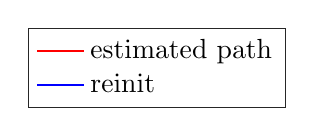
\begin{tikzpicture}

\begin{axis}[%
width=0.951\figurewidth,
height=\figureheight,
at={(0\figurewidth,0\figureheight)},
scale only axis,
xmin=-487.434587954314,
xmax=433.186619595571,
ymin=-17.60491,
ymax=708.497945632086,
axis background/.style={fill=white},
legend style={legend cell align=left, align=left, draw=white!15!black}
]
\addplot [color=red, forget plot]
  table[row sep=crcr]{%
-0.0254918464850879	1.53029535298812\\
-0.0249375910222026	1.94734709129116\\
-0.0603236978857134	2.6546735108884\\
-0.0898810439677802	3.26129873758476\\
-0.122075910018214	3.77863002775995\\
-0.159570842980351	5.84214038823406\\
-0.162924757869628	7.08369056436346\\
-0.345776789656578	7.86663308840249\\
-0.274915939891177	8.64211113562301\\
-0.309598017917685	9.85377995390351\\
-0.277110670012233	10.8074353831107\\
-0.341823185024733	11.5749687633776\\
-0.217611982003351	12.8917266019904\\
-0.0592982609196149	14.535514156623\\
-0.180911942853752	15.86511539354\\
-0.297283259467498	17.8330042136393\\
-0.412075349790875	18.7361261341307\\
-0.45753291768454	19.5761622770474\\
-0.621156244022164	21.0674957763717\\
-0.980582354759486	22.4156368973729\\
-1.22745431999006	23.3028125720513\\
-1.40193957398277	23.7818677316401\\
-1.65427238796997	24.791386743011\\
-1.52909943759902	24.9025031226846\\
-2.10890838431986	26.4020438346825\\
-2.19793238221272	28.40001301552\\
-2.23704339166857	29.4186809525608\\
-2.28910190443992	30.3900124930499\\
-2.20457041736477	31.1146611744193\\
-2.32708913736336	32.1942957377651\\
-3.1046891459365	34.5092832958716\\
-2.86666787719013	35.0211068413269\\
-3.12788023223491	36.3340656885707\\
-3.14026022644418	36.6844767137332\\
-3.1763230709074	37.6947346947444\\
-3.19495295473727	39.7325365835177\\
-3.1999146216173	40.5911151331123\\
-2.97344909913151	41.063906280816\\
-3.40384290258881	42.2966152240875\\
-3.47924892539077	42.2907912175092\\
-3.51533912492827	42.9128038773516\\
-3.41220774206901	43.2871672008606\\
-3.43107682645558	43.8841031817051\\
-3.3802805989678	44.4899463276185\\
-3.41780365850723	45.290609752567\\
-3.56538457932131	47.2700071947444\\
-3.54170874188804	48.3231399669896\\
-3.51872795299972	49.4270266608938\\
-3.60244169429268	49.7658040574899\\
-3.55069899346382	51.0677720338937\\
-4.06169228148522	51.8985114628281\\
-3.87716772743431	52.3325128768682\\
-4.03676201030629	53.3121159711052\\
-4.23660148659786	53.4716323302643\\
-4.310275694325	54.4634466306951\\
-4.46041807929603	56.3401119941697\\
-4.39766273411414	57.3330705926144\\
-4.47541828356611	58.2568629130125\\
-4.68476592208113	58.8044288524739\\
-4.96337870390496	58.5337065180881\\
-4.85996654966614	58.8330834417471\\
-4.7452852030181	59.377853740373\\
-4.80411976120381	59.7694113168104\\
-4.97958983966172	60.1432801036768\\
-5.33346203452014	60.8827166528401\\
-5.40881217868839	62.9197013483226\\
-5.38299725718005	63.8770884548293\\
-5.46894375270949	65.0352800411604\\
-5.44658793859153	66.2969757605726\\
-5.59682216374223	66.8794835318977\\
-5.62515761682646	67.7375248327186\\
-5.82959572590435	68.4174121467227\\
-6.11969249048862	69.1220348180013\\
-6.34944375114614	69.9228287278308\\
-6.20242684256652	70.0229473953826\\
-6.26216603060527	71.8929985190301\\
-6.53240598460052	73.0484201443407\\
-6.68058298346214	73.81860351372\\
-6.24471592205761	74.7407053864734\\
-6.58653996713551	75.4780105178333\\
-6.83556320132052	76.9078142307244\\
-7.45304607736485	77.515645987006\\
-7.2703481830243	78.9468140478602\\
-7.96764211135368	79.8792750291977\\
-7.90195609934829	80.3869994667202\\
-7.48347346531456	82.2250742149803\\
-7.41904012546846	82.9855866278365\\
-7.62222165570713	83.3189114646851\\
-6.66054976290961	85.1642760418981\\
-5.92372458727007	86.0510392104965\\
-5.37255321179372	86.7804206004575\\
-4.82698639480489	87.3534270006329\\
-4.05882638420793	87.9518016292051\\
-3.42049266570034	88.4878692136315\\
-3.07319374126508	89.5378490439526\\
-2.49555476325734	89.9140803042983\\
-1.82720330928408	90.579330152295\\
-1.06245231197866	91.0147293444746\\
0.831161624023544	91.6830870397859\\
1.92220318835705	92.0562525516675\\
2.703405356295	92.344511889211\\
3.09553111825779	92.6807645537764\\
3.47833441856249	92.8206990203711\\
5.03469423672586	93.0767547859246\\
5.9575724714118	93.1118443983965\\
6.7411978337854	93.2705287316002\\
7.33962038308323	93.3476808642605\\
6.35372092578588	93.1201383463387\\
8.38842701723895	93.0943290328837\\
9.34929611611157	93.0279357682109\\
10.5204950530306	93.1287326523483\\
10.4391271302333	93.0108510622458\\
11.5781392250822	93.0920806699144\\
12.5879476899804	92.5940850021238\\
12.8653732510377	92.7978199966934\\
12.4770197191745	92.7788123201583\\
13.3402727086149	92.6515437093406\\
14.8475027339333	93.0884899157036\\
16.9849525157294	92.886685501215\\
17.9424292394414	92.6769790623989\\
18.8756017463721	92.4383972772144\\
20.2367984346504	92.411798365746\\
20.1553283542932	92.3537124400252\\
21.7303960287518	92.4231034488387\\
22.318811700132	92.3703987842169\\
23.2843221942624	92.5736813911858\\
23.5476425836113	92.4444898290878\\
24.7217374947218	92.0439333441509\\
26.6246867149605	91.8892799974856\\
27.6852714119599	91.9389416510773\\
28.4966260945544	91.6614847987351\\
29.5452932188512	91.7617450197497\\
30.799154831897	91.7594498188878\\
31.4843169064553	91.5924953182526\\
31.5101389223031	91.4803098348876\\
32.9103068276762	91.4625820569122\\
34.0554287102297	91.7108536498233\\
34.854245467694	91.3885737334176\\
37.0064062505207	91.2332616468942\\
37.8962788461942	90.8677773738186\\
39.139874133317	91.0514750992464\\
40.3620106324191	91.1120671024734\\
41.3316973678296	90.8630333670727\\
41.9573034455163	90.8744570690545\\
42.7579826172021	90.7489224535197\\
43.4611774118825	90.6951250152443\\
43.9787896487935	90.5964367353479\\
44.8248443685786	90.4400976882435\\
46.843688153292	90.2375043956527\\
48.0430647141051	90.0276360409063\\
48.7947919319514	89.9632979523678\\
49.4018255306957	89.7430620142457\\
50.469233256733	89.4196559409906\\
51.3338779321121	89.4703480171362\\
52.2673239379996	89.2126247804107\\
53.4877674667263	89.0206987142172\\
54.4454250379729	88.782713216564\\
54.8083181248284	88.6838926619963\\
56.8475790680907	88.1379335659271\\
57.8779583313881	87.8408676893505\\
58.7603211069591	87.6627985468884\\
59.1862085071135	87.4043607143007\\
60.1829504861247	87.2365261971715\\
60.6260103760814	86.9318873808308\\
61.5467548780768	87.0752318278574\\
62.0118343353985	86.9408531218701\\
63.2034583688849	86.5724606615819\\
63.3584020011834	86.6492134167508\\
65.3045822540945	86.2283934117083\\
66.2280277718835	86.1390668939848\\
67.3401995166535	85.9915222833997\\
68.2602822355772	86.0400601610079\\
69.3908656496828	85.8166323872064\\
70.480434223319	85.8472621364801\\
71.4590927625654	85.860784171599\\
71.8984784446519	85.8432561909549\\
73.017600928979	85.9720100514982\\
73.5664205129211	85.991553859444\\
75.3779751150422	86.462836433927\\
76.3930628061469	86.7585148999059\\
78.1522033973923	87.5529752613964\\
78.9059446515129	88.148159806268\\
79.4394229160206	88.5565811480382\\
81.0164912684306	89.7166830920654\\
81.7748629783018	90.4045079238118\\
82.5774627369265	91.0046254182981\\
83.0635624808822	91.8548277415086\\
83.0472228654165	92.2327607645176\\
83.4735071312159	92.8029343735561\\
83.8368571083184	93.4137115299865\\
84.0388778404357	94.3455001748971\\
84.3150049121633	94.8151380239427\\
84.474604022441	95.3427819255749\\
85.2442883752967	97.1853600936987\\
85.6387865843154	97.9565795568232\\
86.1026069926334	98.7036322452239\\
86.2068078635372	99.8305982794565\\
86.8911876410266	100.840907739674\\
86.933598166186	101.071293329344\\
87.4673240288864	102.368084568331\\
87.525192740656	103.075132381379\\
87.8043556129768	103.749443146107\\
87.9322167116902	103.77157352176\\
88.5708067335136	105.407863163385\\
88.8621554236845	106.202881049857\\
89.3473294728564	107.052896079122\\
89.6312331025164	107.825694518476\\
90.1950798647475	108.832752930519\\
90.4726819758715	109.402757420469\\
90.9384340360515	110.160027895917\\
91.329349382565	111.248927131879\\
91.6046048597881	111.483428422796\\
91.7943277671	112.263623224876\\
92.6539537890518	114.090887990512\\
93.0817556447811	115.156930483329\\
93.1864705565478	116.180710805326\\
93.5300253835059	117.357094763335\\
94.1775693393444	118.122779210298\\
94.8118427502756	119.304174888303\\
95.2207260808372	120.063077801065\\
95.5141052435902	121.242404593147\\
95.5408157853927	122.329030552254\\
96.0024575867034	122.896302827327\\
96.7321943264813	124.638166935749\\
97.0240393263921	125.621999845097\\
97.1235291808986	126.429637564541\\
97.4234322977447	127.276105940728\\
97.9858149577917	128.169668051469\\
98.1802043049132	128.932181514332\\
98.6951839978977	130.10879710769\\
99.1195433102156	130.87280349267\\
99.3690678808201	131.807716746729\\
99.7811652080873	132.389592639413\\
100.450687377278	134.245153760661\\
100.883293893408	135.104151058616\\
101.228494648544	135.503172478999\\
101.619998696119	136.69779306347\\
102.125350416227	137.44657220391\\
102.231652922542	138.181910488649\\
102.812382253468	139.13991918374\\
103.104727827008	140.254362244662\\
103.296776588324	140.75292747138\\
104.139746689705	142.276159902178\\
104.86087232899	144.001264204568\\
105.39976008317	144.887974951932\\
105.614341679909	146.000958797047\\
105.310006986904	146.3640419368\\
106.06015544436	147.666338661284\\
107.496217823598	148.963948274834\\
107.697000364526	150.017735368443\\
107.427552065836	150.511625085049\\
107.571386141893	151.312023784861\\
108.00449554998	152.499786781213\\
108.305058063586	154.023399384193\\
108.338488685362	154.822527631891\\
108.290133312481	155.58044885632\\
108.643782658208	156.436116253598\\
108.961990515287	157.329572252915\\
108.756165410659	157.582557643443\\
109.18162841614	158.73286037655\\
109.278436428526	159.303975688974\\
109.994110795036	159.655288071485\\
110.194007332468	160.510160589064\\
110.671937113968	162.269735321779\\
110.974417060585	163.131925990121\\
111.003904813808	163.96106280492\\
111.199640897613	164.998124492546\\
111.369192314654	165.759141281454\\
111.632262563028	166.299490138208\\
112.190513657522	166.731790341997\\
112.250633151161	167.435073966826\\
112.244187949632	168.224587440406\\
111.994815130392	169.245324470362\\
112.465992764527	171.06318993158\\
112.560914801692	171.888463612167\\
112.829094846379	172.888889986235\\
112.905183706172	173.401129371306\\
113.320262927833	174.219275475828\\
113.562895166033	174.920831367866\\
113.897531881391	175.776169462335\\
113.790897095294	176.350639187626\\
114.136403318304	177.032969640445\\
114.682963817345	177.801578932885\\
114.886654496916	179.844477827036\\
115.076877779387	180.708172471441\\
115.139905179756	181.594696317361\\
115.120856873685	182.614676178458\\
115.091670417005	183.454158836478\\
115.0824649163	184.333450561979\\
115.146209163667	185.472873647006\\
115.511640924641	185.54016050346\\
115.327808250321	186.851456393392\\
115.556487231236	187.79902389675\\
115.554999418745	189.8370487022\\
115.58971320191	190.784568771652\\
115.697695820703	191.660994672091\\
115.624453407308	192.800338404278\\
115.813686931741	193.558682897847\\
115.808831876937	194.497524225237\\
115.539343133131	195.053582196225\\
115.69006118187	195.862133659747\\
115.783766497445	195.957176789973\\
115.745122351758	196.79867366274\\
115.749536301601	198.829883502489\\
115.76317000853	199.759506981399\\
115.677097255926	200.766270026226\\
115.907496840404	201.69282744845\\
115.88116352653	202.408572461786\\
115.99623083769	204.449041174829\\
116.076150698429	205.800153217535\\
116.19831937405	205.960895698162\\
116.029511705086	207.435846067016\\
115.972146256106	207.839796592752\\
116.053168001555	207.978485719945\\
115.972908427587	208.524840621331\\
115.991810339631	209.025539850117\\
115.987946373916	209.704708549209\\
116.04907770346	210.137519904091\\
116.130816297273	211.868929834897\\
115.999558433313	212.783070913674\\
116.076925348493	213.693929723924\\
116.186680122058	214.591416883041\\
116.199773192846	215.151767187683\\
116.281850783526	215.822257703164\\
116.290342860868	216.873802680422\\
116.403185479788	217.652205661934\\
116.551465829794	218.220972776365\\
116.689989648986	218.836156720721\\
116.942521105905	220.685956952216\\
117.03777241833	221.683027673394\\
117.088138155972	222.875840033326\\
117.103663598687	223.78536483767\\
117.304485719973	224.752740899026\\
117.286520727893	226.252208666781\\
117.446556881851	227.118644230433\\
117.378041459464	227.509644082656\\
117.715919180864	228.206447729935\\
117.3532136922	228.016877268225\\
117.586999079945	229.99330052126\\
117.693686976663	230.728551907634\\
117.762485890061	231.736870182533\\
117.98455337501	232.723327590384\\
118.194911902297	233.703918942658\\
118.227744706909	234.565123943069\\
118.540329726977	236.029496498554\\
118.617985971574	236.85565426124\\
118.747401574653	237.252164981047\\
118.414602297102	237.224408805884\\
118.604512316579	239.140044513402\\
118.760695751684	240.055594272712\\
118.614310404732	241.096334657309\\
118.030414937293	242.525930954227\\
117.902659708883	243.60803169743\\
118.246839649447	244.393616067411\\
118.225504895556	245.335397107624\\
118.388174465246	246.396128462897\\
118.24497479013	247.174524693814\\
118.236957352339	248.458770872379\\
118.520652671598	250.261108834221\\
118.610949150365	251.13321616661\\
118.565803534959	252.127790833849\\
118.458197623691	253.101756805564\\
118.172953268865	252.944971406507\\
118.451150364981	253.749259656234\\
118.507660892166	254.281709159916\\
118.565121616765	254.524306896993\\
118.561367480894	254.837787316879\\
118.749427325962	255.524079572927\\
118.724171852597	257.381091430706\\
118.484388792594	258.182109210627\\
118.556027616311	259.109427374677\\
118.165759598545	260.021205200157\\
117.879272415803	260.554613731055\\
117.748260023955	261.395784522678\\
117.422726365583	262.056882681848\\
117.039306734922	261.8442919051\\
117.171527118565	261.481170887724\\
116.755016592647	259.64635364983\\
115.465019725894	260.993354830399\\
114.995323969316	261.353813856106\\
113.840129982225	261.988160820946\\
113.283496124612	262.238861203577\\
113.029857848354	262.798749220933\\
112.581267173431	262.939834544644\\
112.26991602315	262.98846468398\\
111.951474930107	262.915300993348\\
111.449196544098	263.117552950245\\
110.904665185541	263.455512227186\\
110.678941333669	263.564031782753\\
110.466913506337	263.646839845568\\
108.330077757507	263.854485693942\\
107.336908006412	264.033218723538\\
107.149864308116	264.050522259474\\
105.910760434938	264.381168786507\\
104.888207673094	264.53798438298\\
103.712570246785	264.635817406925\\
102.65562166413	264.834120296913\\
100.723843504699	265.583524777361\\
99.9993580250268	265.550604991516\\
98.4848770401361	265.606230294445\\
96.4572046873498	265.700537614421\\
95.4589935407263	265.899119497044\\
94.7159349880924	266.07634823999\\
93.9670981118293	266.158105439125\\
92.6126836910795	266.313135423089\\
90.5189547799521	266.394669167175\\
89.8496238937281	266.418424419081\\
88.496716558052	266.422058071013\\
87.5469312835718	266.70810121802\\
86.5748906268413	267.213011720361\\
85.0297340729904	267.634318608119\\
83.3004349664897	267.743973897421\\
82.8372375607338	267.968818669733\\
81.5257554572338	268.676876050794\\
80.3724051074627	268.826073135915\\
78.3337098077821	268.948632085626\\
77.4092606501856	268.57307814095\\
76.2594266732358	268.838544814538\\
75.6719055031984	268.944235037161\\
74.8007841950479	269.118655517727\\
73.8513110717585	269.107582044551\\
73.5387435261417	268.93444647877\\
72.821911261984	269.017919827982\\
72.1747004650987	269.206536353585\\
71.15378459574	269.579705306292\\
69.2024781676488	269.518136769483\\
68.3887294177064	269.473368681728\\
67.5897160868135	269.319154353423\\
66.8308491793402	269.241701459402\\
66.1755492862452	269.42695776203\\
65.9321387373286	269.41937188911\\
64.9877436397125	269.435034329034\\
64.4665974670496	269.358980892031\\
63.7699497041024	269.373671090927\\
63.3161513911275	269.357726527924\\
61.5027941484165	269.45229332111\\
60.553363933439	269.338963103192\\
59.9287920537787	269.416810907786\\
59.1347968221773	269.400209022955\\
58.3079807399822	269.437813771495\\
58.264494617748	269.327957022512\\
57.6650301328798	269.225708496888\\
57.1344328688458	269.277616040591\\
56.624744528847	269.301378211897\\
55.9699315080572	269.229784124547\\
54.2591881403599	269.112891166674\\
53.6577534516803	269.031923508574\\
52.9875873718299	269.110359232275\\
52.0638056797522	269.088310985081\\
51.4247230093222	268.939227076469\\
50.7654006295958	269.113230737356\\
50.7328568005023	269.248274405194\\
50.4909574797099	269.279682794771\\
49.9299518999195	269.355499116522\\
49.2705800567838	269.527646249968\\
47.3531622336715	269.24433452203\\
46.8023762427284	269.48247858706\\
46.0832908224132	269.506812385887\\
45.184193529931	269.549390918755\\
44.7642791049058	269.400858640935\\
44.3816236512892	269.228083741288\\
43.6144290749945	269.265222767433\\
42.8303619605763	269.325637743007\\
42.0642024541579	269.473099246193\\
41.49429912792	269.292464975344\\
39.5672410211106	269.311191892602\\
38.9971107482665	269.466344929805\\
38.0821660089989	269.386981012965\\
37.5009281710199	269.802758846237\\
36.8963468327465	268.995578577947\\
36.1722180307312	269.539284579348\\
35.3269166144196	269.858632952252\\
34.6825069483238	270.200278790423\\
34.06623121852	270.019705590972\\
33.9019549409514	270.029601612212\\
32.6256808871999	270.048863565557\\
32.3162334272419	270.124722591184\\
31.7378004062333	270.273369403073\\
31.3860253593739	270.101385144902\\
31.117149335736	270.155732348942\\
30.9447731222826	270.263843308243\\
30.9695145685314	270.384897981527\\
31.2056501381599	270.411147756973\\
31.0329761094042	270.376128776436\\
30.8160939073723	270.47642619321\\
30.2451124139603	270.230628590634\\
30.118457684618	270.320824324765\\
30.2866159834956	270.306526517509\\
30.2213363125871	270.293967582896\\
30.1898360760918	270.264969227862\\
30.1671410800629	270.26605041667\\
30.1445843408197	270.279043813379\\
30.2197334065304	270.294011434097\\
30.2284534262905	270.290063672298\\
30.3120940886391	270.291773405456\\
30.4380357400992	270.319183836018\\
30.5959622314036	270.293006001129\\
30.4035669585637	270.562894521129\\
26.9091396392751	270.481533203549\\
-2.28223663172593	254.32979324142\\
10.9793784076891	265.340723472528\\
-6.85408007680556	255.041138653325\\
-28.8259267063358	262.622888997367\\
-49.6798231945613	271.129647182125\\
-64.6786215126092	296.413835634583\\
-65.124770945043	296.066192287026\\
-65.5903691382669	295.83715961396\\
-65.6701160933635	295.616807769682\\
-66.0555967413566	295.738199855184\\
-66.2467223046052	296.011798228188\\
-66.303443797322	296.108363007127\\
-66.5737776161598	295.977631515247\\
-66.8091687754275	295.756129740389\\
-67.0689094837122	295.947734703503\\
-67.2264983337518	296.002507526586\\
-68.4075810669247	296.252603100057\\
-68.6215903521132	296.487066164511\\
-69.1429622988055	296.706844336415\\
-69.5686228909828	296.986999347364\\
-69.8136110272821	297.49523904283\\
-70.6645908775846	297.589243269733\\
-71.1512976648205	297.998783840728\\
-71.6793447475805	298.095991495961\\
-71.925898456987	298.671185206105\\
-72.2139225915154	299.354806423241\\
-73.3276133320711	301.065882171282\\
-73.6261935383027	301.835456811125\\
-74.1103304535596	302.735266006414\\
-74.230132948668	303.257735685215\\
-74.3485525304665	304.094130519068\\
-74.7557320963988	304.996255441233\\
-75.316517003935	305.975480079551\\
-75.9028849145566	306.816329871484\\
-75.6074017884892	307.643798205075\\
-76.2460828676138	309.303984152877\\
-76.2771456405465	311.412815171714\\
-76.0984942642432	312.582503923003\\
-75.7631049747394	312.663045431974\\
-76.3991395741126	313.397218220734\\
-76.2669191873069	313.378679351442\\
-76.4384229184186	314.839558915385\\
-76.3267381673152	315.824631192676\\
-75.7392991334047	316.367652049915\\
-76.1405831191092	316.603963816132\\
-76.1698029984719	317.630019428446\\
-75.995038791915	319.556614203893\\
-75.9428178577284	320.548465274719\\
-75.7980101042201	321.466312676737\\
-75.9507812332651	323.049917649067\\
-75.9659006357565	324.036654823488\\
-76.4101445441579	324.883768820789\\
-76.3555950383185	325.979983858377\\
-76.1277649447853	326.248061362135\\
-76.2894634086737	327.852579268551\\
-76.9395410905887	328.791853243335\\
-76.6316716216146	330.755441149705\\
-76.4731813748364	331.803754518199\\
-76.4339257112383	332.767217769585\\
-76.8921137346341	334.601017991717\\
-76.9415614793641	335.199926264902\\
-77.2412057284686	335.729539150348\\
-77.7695953548005	337.11859001213\\
-78.0654867196582	338.084893192498\\
-78.0497758362596	340.046321231407\\
-78.4367259738144	340.871640607924\\
-78.1077422889772	342.642404384994\\
-77.9420177818172	343.754723934489\\
-77.9620733732278	343.087985433572\\
-77.979595687369	343.704812558846\\
-77.9175294095477	344.110084493764\\
-77.9855456333866	344.698114111034\\
-77.952920210987	345.051496703742\\
-78.0450730679235	345.493864049856\\
-78.0179167737445	345.782744137279\\
-78.1474855463623	346.204608501658\\
-77.4575172329224	348.994171405354\\
-77.2502921425738	350.074979110665\\
-77.0089542173353	350.895639606808\\
-76.9016016841993	352.00990855535\\
-76.7273481508357	352.341942890554\\
-76.3904764829653	353.220540368779\\
-76.1461140044755	354.012480103343\\
-76.1048517499306	354.537532790811\\
-76.0286397737368	355.064597899069\\
-75.7681190956068	355.688103372868\\
-75.3710346861287	357.646385555002\\
-75.0496987189043	358.742810626347\\
-75.0458474691312	358.990747312311\\
-74.7019730346898	360.028350997941\\
-74.6579610971285	360.660384481105\\
-74.3146815188492	361.570319730334\\
-74.0359027480128	362.485482837638\\
-73.8045198386295	363.339544311956\\
-73.6334609381254	364.073078399777\\
-73.5324136779428	364.920381756145\\
-73.1144173531488	366.718492182456\\
-72.9904827551441	367.569577771054\\
-72.5221486263914	368.450394119453\\
-72.4380746698509	369.455225510193\\
-72.1713744576287	370.129377535496\\
-71.659226031202	371.277236505105\\
-71.4417491130633	371.95647995622\\
-71.0309889267264	372.973186550883\\
-70.9706938732837	373.62925967342\\
-70.6087462005576	374.576103078844\\
-70.2888134292997	376.438255024424\\
-70.0560684195522	377.419439313939\\
-69.8759357849143	378.41840258046\\
-69.5751792448718	379.355559087107\\
-69.2886466150511	380.282353024432\\
-69.0471203302677	381.168019815369\\
-68.8005896678043	382.033259263562\\
-68.7199740409364	382.996583123071\\
-68.0907861794999	384.313437388493\\
-67.5039358555616	385.204176879401\\
-66.961876955991	387.181235877653\\
-66.8015059330995	388.017482882041\\
-66.6271932326837	389.087319153829\\
-66.3584146839575	389.963366000891\\
-66.3724877723002	391.260473867763\\
-66.2177699796688	393.287315432267\\
-65.8525149055688	393.998643262218\\
-65.6673368531899	394.972913385406\\
-65.4409664231543	395.663795163106\\
-65.1889996945767	397.54259756338\\
-64.9309047959747	398.392960670221\\
-64.9933200773193	398.889246742445\\
-64.6990072624691	399.823139627584\\
-64.4174438674856	400.596178093109\\
-64.2608650555732	401.562380759736\\
-64.9200437909872	401.06816151101\\
-64.5121875450677	402.19667078648\\
-64.4501786907455	402.828021572913\\
-64.9178076440124	402.62940016046\\
-64.6400664540925	404.480207435174\\
-64.1050190520493	405.423351702974\\
-63.8737171845338	406.631141963572\\
-64.0597574671072	407.580376161906\\
-64.1738577942516	408.721401021287\\
-64.3496898994273	409.39357572293\\
-64.2145899059231	410.214570425765\\
-64.3170852353316	411.081147615821\\
-64.3923916444166	411.86487321246\\
-64.1835748482841	412.37930129828\\
-63.8479712999405	414.164791302417\\
-63.4803411869382	415.178697055701\\
-63.8632870257144	416.403023826442\\
-63.4338862793661	417.073861311429\\
-63.7358418662253	418.363481254471\\
-63.5611293336481	419.003232364372\\
-63.1906064829005	419.772927584999\\
-63.6819631259794	420.766356936413\\
-63.7119024957913	420.665808075166\\
-63.4838564187163	421.135291835563\\
-63.2755945376052	423.00391537795\\
-63.4307616844695	423.883988014606\\
-63.5188738884758	424.842317934327\\
-63.9010243027514	425.503737043815\\
-64.1589476916236	426.267526530192\\
-64.6995322159818	426.929061037671\\
-64.9181459657262	427.37625023897\\
-64.93371772688	428.030702451217\\
-65.4602478486647	428.864018365596\\
-65.9113640338545	429.286913052086\\
-66.9054315699656	430.553715354392\\
-67.67780558457	431.451723045333\\
-68.224130037433	432.09893850109\\
-68.8550485815686	432.567234314089\\
-69.7389701128695	433.11261251955\\
-70.6259811450643	433.623166250557\\
-71.7503097026518	434.318378149082\\
-72.3263347205629	434.204826315416\\
-74.1435076642217	434.781672340058\\
-75.109995899111	435.18096226697\\
-75.8886369738461	435.568746303269\\
-77.2256137136003	435.905972114918\\
-77.939945400346	436.374254862393\\
-79.5420910578802	436.942133721828\\
-81.786295139055	437.170769684038\\
-82.924389147786	437.027008458666\\
-84.0880597467881	436.761041964314\\
-86.1402005779807	436.898369768652\\
-86.9331477423677	436.462929467833\\
-88.1623518998726	436.833564311918\\
-89.5201269041378	436.560372109224\\
-90.9269069927792	436.608511402841\\
-91.5808442377659	436.818344073232\\
-91.7764310879927	436.961592097465\\
-93.9329403132604	437.12670524348\\
-95.6521300502414	436.957467210372\\
-96.6751968679617	436.756800565515\\
-98.6177877928952	436.808676939825\\
-99.7842358164489	436.896945234294\\
-100.188096194897	436.951064054841\\
-101.561499599844	436.916534198177\\
-102.306718818729	437.016890164376\\
-103.441090868503	436.99889023756\\
-104.285211803317	437.236591897237\\
-104.471448405851	437.315821649894\\
-104.785852082435	436.894047531991\\
-105.507267440735	437.06001294959\\
-107.425561886017	437.210335590078\\
-107.933361955093	437.427852949242\\
-108.901679070217	437.437946833927\\
-110.051642098623	437.44414271632\\
-109.677074607031	437.317882146123\\
-110.313368457199	437.649603197321\\
-111.985674562022	437.7758889818\\
-112.778898168852	437.894859517145\\
-113.318294729286	438.008096775166\\
-114.019395796528	438.115595886385\\
-114.853144510546	438.075342840568\\
-115.533014145717	438.095854624122\\
-116.195697112306	438.337909894452\\
-116.745053984119	438.471734065638\\
-117.47424347537	438.574032815747\\
-117.904222282424	438.751020039133\\
-119.657690843945	438.812580347651\\
-120.588732572699	438.881333149762\\
-121.56644465437	439.006517490273\\
-122.120640575411	439.276978668387\\
-122.869025849187	439.288076724836\\
-123.555765556612	439.482458345553\\
-124.162174416434	439.416740749323\\
-124.691508175911	439.466464274671\\
-125.673676787964	439.485015810398\\
-126.263477670564	439.430159167169\\
-127.952031170072	439.574605642332\\
-128.94273292514	439.579491632791\\
-129.472439759851	439.737042566798\\
-130.357428373163	439.713956079063\\
-131.162595344122	439.851683706287\\
-132.09142043118	440.069696564574\\
-132.656943565044	439.993231405274\\
-133.573125900975	440.434000026713\\
-134.483854855574	440.267211622338\\
-135.149823805386	440.456198102748\\
-137.036460621226	440.608897600244\\
-137.662136226304	440.638669215476\\
-138.327816706073	440.56054084022\\
-139.264149779602	440.852948421595\\
-140.078309683881	441.128550887051\\
-141.109402491492	441.202618668386\\
-141.961183111285	441.305455176931\\
-142.579818237418	441.703437664825\\
-143.353334456878	441.529572202941\\
-144.100139406953	441.895447588775\\
-146.059254571708	442.076737491464\\
-147.071157657854	441.947217499347\\
-148.017458243145	441.949353411453\\
-148.943730393739	442.244328594144\\
-149.841014540522	442.34320449909\\
-150.597565843705	442.607155657494\\
-152.261364207796	442.7838614072\\
-153.132500510573	442.598412681822\\
-153.668665334871	442.420827891284\\
-154.750072581498	442.76440717349\\
-156.837273678706	442.689382136577\\
-158.020971038702	442.587058238925\\
-158.484533835585	443.086600594036\\
-159.749120713955	442.646274977709\\
-160.958411143064	443.040936544902\\
-162.591993471635	442.5746837027\\
-162.673281519053	442.588693411468\\
-164.054095935982	442.72673337226\\
-164.300971169419	442.503056904546\\
-164.974590424103	442.76981659125\\
-165.646818588093	442.843547833041\\
-166.278525557952	442.947464206105\\
-166.426138874688	442.896959092424\\
-166.933903451853	443.103555640656\\
-167.496756246275	443.188424706388\\
-168.065312848754	443.329005062301\\
-168.511336464068	443.219825722839\\
-170.58702486405	443.254517922448\\
-171.629344681495	443.25084965799\\
-172.365288764564	443.366416707518\\
-173.575201284587	442.991293059986\\
-174.784060069065	442.786260788591\\
-175.6825441608	442.870339481838\\
-176.799729140358	443.342077654937\\
-178.314816214258	443.953280720804\\
-179.364701354693	443.546873962273\\
-180.629654963074	444.01568761642\\
-182.565482358743	444.073331879712\\
-183.06165131966	444.072380515048\\
-184.231115768158	443.976098905836\\
-184.93977516777	444.121834720409\\
-185.966253203488	444.002137236096\\
-186.717975095755	443.900184122538\\
-187.876697217151	444.351636688678\\
-188.619694872601	444.349352127726\\
-189.245413276463	444.456427796804\\
-190.293293730251	444.53854748671\\
-192.308452708666	444.56608141255\\
-193.08282017347	444.421017865619\\
-194.260791888043	444.702515653869\\
-195.581779695126	445.295530685341\\
-197.009947890621	445.44428685466\\
-198.069776354849	445.829832520068\\
-199.337633673995	445.33467224199\\
-200.532542820607	445.379970265999\\
-201.802423420644	445.538738892709\\
-202.697911090418	445.789619541805\\
-204.517396358439	445.514200645263\\
-205.111041983583	445.476167900141\\
-206.792044483587	445.227403853286\\
-207.418151363314	445.105627498001\\
-208.748940276764	445.647799710813\\
-209.350248108045	445.490089730179\\
-210.103115097554	445.561798629223\\
-211.986093602072	445.245649253291\\
-213.12342796677	445.07023551066\\
-214.211060509468	444.918012340218\\
-215.052067652435	444.93037468798\\
-215.852503059306	444.675571295379\\
-217.12009197074	444.576618865115\\
-217.903999481996	444.436165362752\\
-218.82402199816	444.368115685013\\
-219.675582337758	444.150202403976\\
-220.730119072232	444.192502069521\\
-222.592211065748	443.971314768009\\
-223.332147108949	443.89968486886\\
-224.025141177008	443.476440874928\\
-224.958578171184	443.446576300252\\
-226.148966524606	443.445320749321\\
-226.824977074099	443.258422772149\\
-227.434255186124	443.30989567361\\
-228.125716295857	443.117730184319\\
-229.204079532249	443.097834624975\\
-230.539196108658	443.581172674108\\
-232.495261026184	443.364578926453\\
-233.267433068548	443.253547717979\\
-234.763178493114	442.621527067267\\
-236.671574487075	442.076392967796\\
-238.038043647739	442.134093059681\\
-239.493255050599	441.827713328115\\
-240.397990820171	441.763777032551\\
-241.551006298017	441.46418190228\\
-242.964694898299	440.816569445718\\
-244.171442895953	440.756797248728\\
-245.975005383314	440.465957667118\\
-246.905986379903	439.964415545569\\
-247.932113637914	439.639699594229\\
-248.368312534858	439.274945994651\\
-249.16840080447	439.141116028687\\
-249.891521805785	439.186409245787\\
-250.553020246338	438.639810669839\\
-251.278969439344	438.398920326922\\
-252.777687301388	437.228047148506\\
-253.531009677055	436.463804076988\\
-254.117763829143	436.101967766234\\
-254.596439856359	435.322271242405\\
-255.176185679854	434.749232483194\\
-255.779727819807	433.877032963131\\
-256.0896791091	433.095765267647\\
-256.736340293971	431.947544744422\\
-257.332485935629	430.18025163895\\
-257.70036179116	429.044038624538\\
-257.707102169845	428.216682223346\\
-257.960932235131	426.979719290515\\
-257.98968819805	425.771484504081\\
-258.165763343115	424.030255852674\\
-257.952608080796	423.202044993914\\
-257.610741544772	422.101797859614\\
-257.411641698251	420.163159956702\\
-257.605130661993	418.423755033327\\
-257.442774588347	416.496391205844\\
-257.368509110662	415.596867432151\\
-257.142453163388	414.684670780963\\
-257.177876070896	413.716015866271\\
-256.853805118204	412.516456367083\\
-256.579706091866	411.616087639965\\
-256.561699547676	410.428035173742\\
-256.756102324209	408.963739406727\\
-256.459140759231	407.090680329917\\
-256.061420351511	405.963734092302\\
-255.676597439057	404.855148527061\\
-255.643454228171	404.06989984376\\
-255.518153775211	403.219417935479\\
-255.356022847371	402.334683718171\\
-254.936799113448	400.532216951149\\
-254.754844579912	399.809010517546\\
-254.483591043274	398.863060115858\\
-254.374049651122	397.65192216932\\
-254.151714038179	396.35587052064\\
-254.106391221882	395.603137168651\\
-253.875547513092	395.210272125493\\
-253.64146532574	393.338441770151\\
-253.536671084388	392.50019361273\\
-253.290850417671	392.083424355402\\
-253.045422599676	391.362561006682\\
-253.046372252736	390.342366354298\\
-252.950147331234	389.857591529912\\
-252.809808422354	389.041327496663\\
-252.983417208863	388.642161000236\\
-252.667138832796	388.112966172177\\
-252.636182345479	387.851590884729\\
-252.331236288837	385.964181738267\\
-252.172036928131	385.148471085406\\
-251.826484016386	383.819260922858\\
-251.836971712406	383.566762167831\\
-251.616418997947	382.343685440828\\
-251.434654934891	381.044787330083\\
-251.272527068141	380.890722971504\\
-251.28275431427	380.221560231879\\
-251.167777297991	379.281636203346\\
-251.003854457926	378.579911836416\\
-250.729070852651	376.684449855986\\
-250.513774412411	375.904081497126\\
-250.244422663397	374.772139450453\\
-250.080890980828	373.667021533669\\
-249.975204815775	372.812808634148\\
-249.760615305075	371.113014099169\\
-249.644447879685	370.303038191453\\
-249.686673859931	369.44201127192\\
-249.549068477794	368.59223385088\\
-249.361157208871	367.162710605423\\
-248.979363744584	365.221643360895\\
-248.873160074643	364.335605547528\\
-248.766352154088	363.389938354195\\
-248.59072192211	361.707546420994\\
-248.505687864968	361.334379736518\\
-248.145633972295	359.429895321831\\
-247.985576171121	358.400195547554\\
-247.766179036758	357.60057425073\\
-247.601812174107	356.85859277056\\
-247.458811707774	355.961669284545\\
-247.397098711985	354.768042237921\\
-247.179100422348	353.688565134033\\
-247.62817237945	353.633652154899\\
-246.580770300811	352.722233014138\\
-246.596467745881	351.372402219029\\
-246.265420359809	349.601577529016\\
-246.174007285628	348.593409302466\\
-245.885376520223	347.854124310423\\
-245.888757896242	347.276649226354\\
-246.024575649653	346.873742581339\\
-246.085404770824	346.553639810086\\
-245.65351357292	345.948820175332\\
-245.80129371155	345.326735420853\\
-245.438779375687	344.452511448936\\
-245.442714810742	343.969083324492\\
-245.056905289907	342.034212450898\\
-244.882593992698	340.53155006578\\
-244.690039639743	339.796253535086\\
-244.619931842982	337.644037996212\\
-244.151531671241	337.398703380045\\
-244.118503920209	336.229522205451\\
-243.823925651699	335.125892326907\\
-243.917263098955	333.289073048364\\
-243.888490557472	332.199784783721\\
-243.265742605598	332.209952539619\\
-242.986872716811	330.208297487402\\
-242.682691402616	329.062322894698\\
-242.47096092211	327.862926606306\\
-242.410933949074	326.875728408881\\
-242.289428195673	325.540873804984\\
-241.835571106374	324.377476133931\\
-241.50299608181	322.688181288652\\
-241.368456650596	321.714523992376\\
-241.019379323363	320.903793690718\\
-241.001708278198	320.160701077677\\
-240.938402538336	319.309442485495\\
-240.916942297433	318.407104754417\\
-240.774531742362	317.70733261005\\
-240.481365386626	317.66297943768\\
-240.353667645122	317.378225516883\\
-240.114151551872	316.647725837398\\
-239.700780382113	314.829966473322\\
-239.369063725969	313.773467357159\\
-239.386960523229	312.948351987493\\
-239.069394060113	311.83669041906\\
-238.944627326484	310.800745490465\\
-238.980520098141	311.112371605317\\
-238.796964170733	310.743423799542\\
-238.398372194812	309.311064002113\\
-238.182503008565	308.356270038525\\
-238.119693910587	307.546631919138\\
-237.990622549802	306.471572734215\\
-237.881546496737	305.973198568304\\
-237.379836881406	305.030513418117\\
-237.372894230913	304.111719332791\\
-237.415950207106	304.019121564993\\
-237.306328271938	303.303817296109\\
-237.222717631366	302.598540146053\\
-236.926673319848	301.526781378372\\
-236.853678226762	301.119361493825\\
-236.614439943039	300.192367859258\\
-236.261345895235	298.545803133321\\
-236.209216811479	297.817592605293\\
-236.078937596404	296.568795993458\\
-236.093060091071	295.823052909807\\
-235.556004161491	294.859968508288\\
-235.631123286714	294.094183773816\\
-235.460026120529	293.453204876894\\
-235.295117032036	292.873523889315\\
-235.167732902204	292.118087905405\\
-235.039004141135	291.173573418883\\
-234.680831759537	290.230489241649\\
-234.136715970437	288.696841061886\\
-233.831793456383	287.839278922343\\
-233.614245720766	287.640579866518\\
-232.890621243207	286.417845695543\\
-232.659159462554	283.602605859878\\
-232.49923608791	283.479197292547\\
-232.112027627308	283.285651582488\\
-231.941204305448	284.010893411828\\
-231.466527089189	283.627222101719\\
-229.939029672671	282.413774639911\\
-229.220238355251	281.811706069154\\
-228.256573604365	281.390309463826\\
-227.069397167903	280.741469489204\\
-226.274281760761	280.325101747598\\
-224.734618133423	279.667114117077\\
-223.928234093142	279.604510327893\\
-222.632120625347	279.34745326494\\
-221.738339372846	279.225262675812\\
-221.719093298118	279.173522168872\\
-221.124945268008	279.484644269365\\
-220.409264906511	279.64651775195\\
-220.03494375049	279.57432991524\\
-219.838108370229	279.517148384606\\
-219.482642852534	279.381793528082\\
-217.415644957994	279.633171426786\\
-216.3982710116	279.820104241892\\
-215.311272029464	280.030988988958\\
-214.501081361277	280.076697621746\\
-213.525972088146	280.339019395812\\
-212.040089959492	280.692795774783\\
-210.190965867185	280.892560862321\\
-210.090127859968	280.859736798352\\
-208.707356711329	281.061429640905\\
-207.321205933502	281.370748496254\\
-205.502231331356	281.740014056397\\
-204.507343909026	281.938499202187\\
-203.499307922701	282.157075171693\\
-202.669443545523	282.338992864474\\
-201.333068184852	282.601600527866\\
-200.011500085065	282.922426197495\\
-199.512473381142	283.038715470214\\
-198.013095651717	283.455046349378\\
-197.31847220554	283.60586261933\\
-195.668583919659	283.880326244611\\
-193.639172529597	284.33209273826\\
-192.748462330608	284.558322247219\\
-191.499775481012	284.67922534685\\
-190.640151597712	284.878725079128\\
-190.145734316365	284.9162522065\\
-189.093265522258	285.273460334431\\
-188.296800645074	285.381617495479\\
-187.401263444783	285.676048762025\\
-186.501716026077	285.938516158541\\
-185.707848964496	286.124781439301\\
-183.7765658374	286.660860236443\\
-182.885204419344	286.93046377609\\
-182.050124866054	287.138766652055\\
-181.060270088521	287.389430146795\\
-180.037224737937	287.599402602684\\
-179.093869253549	288.000138578063\\
-178.212005352013	288.193418393098\\
-177.39218626436	288.294206863016\\
-176.80352946234	288.554047799468\\
-175.237433665576	289.050269036808\\
-173.433727872363	289.620024161589\\
-172.95228531864	289.649129414196\\
-172.245042219601	289.913947934346\\
-171.779186336747	289.963846835394\\
-171.258893249464	290.14067043493\\
-170.762002402201	290.218328224509\\
-170.253621535777	290.414676010709\\
-169.628445727447	290.567598336197\\
-169.229848609882	290.660746524689\\
-168.757354639639	290.7755415279\\
-166.878257930997	291.221721143596\\
-166.036814279545	291.382478528897\\
-165.228762669215	291.309911376285\\
-164.671554871732	291.452997764752\\
-163.982684514884	291.596085087377\\
-163.127800218026	291.922817964534\\
-162.081037603522	292.050968578928\\
-161.231977065613	292.280089584524\\
-161.185847093871	292.177716961841\\
-159.114951341914	292.510137164618\\
-158.056684357357	292.598845441862\\
-157.018214044009	292.891037758151\\
-155.871764683345	293.097947988938\\
-155.097617992502	293.044835727453\\
-153.713473977203	293.420123145021\\
-151.716777160795	293.738135893332\\
-150.543326991498	294.196604299298\\
-149.752745441659	294.033779150758\\
-148.621771938168	294.169999435961\\
-147.512189666684	294.717061502398\\
-145.638344511871	295.104280797125\\
-144.52763573148	293.350079048966\\
-141.866264186982	294.405048381566\\
-142.20577586517	295.540772626855\\
-141.344287785125	295.198571390858\\
-139.863050809767	296.45420790355\\
-139.180968028789	297.16532686087\\
-138.494470152618	297.820058943868\\
-137.673283517551	298.753355148805\\
-137.188942517664	299.566450046452\\
-136.688699045829	300.293569712412\\
-136.167814164167	301.233236877236\\
-136.150955663985	301.869434211562\\
-135.519855751695	303.528445870159\\
-135.183736548652	304.225638481569\\
-134.555773318052	306.186794661309\\
-134.359795293888	306.914956946545\\
-134.085727707695	307.967901862458\\
-134.036186505319	309.045859174569\\
-133.916467185181	309.789869238171\\
-133.632518228283	310.869123484259\\
-133.656214427378	311.83699262793\\
-133.772785394911	312.305658763329\\
-133.594305824191	313.497987905522\\
-133.802205270106	314.072070918925\\
-133.801039769163	316.037686937443\\
-133.962631595871	317.041395418596\\
-133.794659572491	317.874675073366\\
-133.851221364931	319.048657156152\\
-133.868334785776	319.666610438524\\
-133.915605603302	320.552269664061\\
-133.72890767304	321.432590166946\\
-133.502123748773	322.417760270977\\
-133.522824733265	323.230082645171\\
-133.312291613376	324.152670612389\\
-132.87613981556	326.022357517709\\
-132.534274254839	327.061118272061\\
-132.181136068536	327.8679815644\\
-131.977508525531	328.246477268773\\
-131.543225385267	329.129128068486\\
-131.123959613547	329.845136040395\\
-130.878056443476	330.581729554788\\
-130.29782139255	331.238344050316\\
-130.165161392545	331.938112937477\\
-130.069279600696	332.596562987946\\
-128.284651338395	333.93088853993\\
-128.039956182691	333.983815597223\\
-127.187891724697	334.492121914386\\
-126.198404382266	335.011566468441\\
-125.10896572104	335.663558960383\\
-123.875916520279	336.496550178352\\
-123.030870394023	336.421565124528\\
-122.102027964932	336.848692067106\\
-122.310250407843	336.611405027904\\
-121.376974507435	337.220905149623\\
-119.595058847028	337.796010213735\\
-118.47822734295	338.243618030229\\
-117.758663061027	338.723803557982\\
-117.069204798494	338.993662169424\\
-116.144144430642	339.13889175381\\
-115.082817211433	339.493498021357\\
-114.159819935066	339.928522611211\\
-113.124794999273	340.572938958439\\
-112.26535074047	340.697490104632\\
-111.83583168297	340.815738911444\\
-110.077003857716	341.298501723553\\
-108.980724048471	341.716109700387\\
-108.21431956541	341.822604754985\\
-107.61880764165	342.33509493309\\
-106.54954845674	342.720035240984\\
-104.556657850715	343.237813996057\\
-103.507457305673	343.524904547107\\
-101.655734773549	344.109825768218\\
-100.790602648286	344.306942201001\\
-97.8676762389676	345.00322434733\\
-97.1317704030728	345.165010515976\\
-95.8392377305007	345.464994795428\\
-94.8582223966113	345.71109431794\\
-94.1600569084363	345.819181194667\\
-93.2735345267619	346.142685504952\\
-92.4802655881318	346.276356084679\\
-91.6259979261932	346.405863962746\\
-89.9054038893548	346.921954355758\\
-90.517826117896	346.41964456459\\
-88.6126617110424	346.824463689944\\
-87.6501429675297	347.023359841044\\
-86.9948647009549	346.959682842706\\
-86.0754796118196	347.166174493751\\
-85.5050499456306	347.408168553823\\
-84.5983695103073	347.701585299332\\
-84.2659524152592	347.545865496394\\
-83.727869834661	347.723663997765\\
-83.0084723604512	347.923393758404\\
-82.5475778998028	347.851645040134\\
-80.9269374407243	348.140323556961\\
-80.5839825859979	348.197334952832\\
-79.6634257549855	348.6149684812\\
-78.568159142299	349.386669229655\\
-78.3480020127951	349.445894152635\\
-77.7773894746643	349.619559229659\\
-77.6702265284654	349.326369829094\\
-76.9155086830353	349.603088815904\\
-76.6685087190022	349.587810329992\\
-76.2104317458032	349.83784288519\\
-73.6814132100546	350.231260248379\\
-72.5375000115908	350.911404224902\\
-70.8736075605844	351.361892922735\\
-69.9391401907612	351.622127998543\\
-68.6474994959417	351.955228426267\\
-67.728457416897	352.172377308862\\
-67.7992938002126	351.814620686109\\
-66.9731321175714	351.832792714808\\
-66.6470460557003	351.942781384493\\
-66.7428686965789	351.710907330902\\
-64.7467837754037	352.192708073991\\
-63.8326674742195	352.400707885137\\
-62.9796926057882	352.575636860938\\
-62.4471349196113	352.136292019775\\
-61.3855781052118	352.715888633835\\
-60.4421216196579	353.021418525115\\
-59.6767620926051	352.67026775866\\
-58.7289783531181	353.189795643899\\
-57.7792242062384	353.337757100141\\
-56.5895870431007	353.554825740164\\
-54.879479832577	354.0313842409\\
-53.9664481426566	354.421820696127\\
-53.4519821086072	354.572544875931\\
-52.7310988157917	354.894108735367\\
-51.9112704594495	355.137201382473\\
-51.3692206966355	355.126772333124\\
-50.5482938929195	355.38364695744\\
-50.1216676293475	355.820759564383\\
-49.338830082358	356.258782907239\\
-48.7608926018094	356.065623703092\\
-46.8864588838148	356.362467272814\\
-46.2812198763906	356.668141742407\\
-45.8624004801956	356.731408517411\\
-45.045403239362	357.601159404577\\
-44.2633761760247	357.179649070974\\
-43.7680640098029	357.319189641397\\
-43.1517498852928	357.912090622791\\
-42.6504786947146	357.869580144548\\
-41.9533885848093	357.737488460797\\
-41.735629940652	357.915303099112\\
-40.6591737294448	358.054869442253\\
-40.4601635135304	358.03377911276\\
-40.154250954242	358.064171208426\\
-39.7252802208479	358.162358556728\\
-39.7092212932055	358.221750925175\\
-39.5968003607147	358.303637010628\\
-39.2529018705919	358.334915050298\\
-39.0020348876553	358.372846598083\\
-38.9943980650469	358.318938754159\\
-38.874826724177	358.193744654909\\
-38.4137079818676	357.823908930021\\
-38.3509876041645	357.732492254222\\
-38.128557177185	357.694377808036\\
-37.8616590884527	357.576911026709\\
-37.6030898139999	357.431039907319\\
-37.4158934957142	357.269835005742\\
-37.1109681761775	357.169190204637\\
-36.8358542315637	357.015006920436\\
-36.6042758084887	356.801725747018\\
-36.8779794755917	357.448360589314\\
-34.9942139736479	357.11923903653\\
-34.7124119354533	356.499806548752\\
-33.9242258071667	356.034071463077\\
-34.9082383705502	355.840608375209\\
-32.8380237946561	354.697850321954\\
-31.4611588881599	353.511095473691\\
-30.7174127678579	352.946812905372\\
-30.7415199235689	352.70186269698\\
-31.3706913432003	352.808442038894\\
-29.6433752815487	351.603967134422\\
-29.256192991611	350.871333396319\\
-29.4641601820774	350.360027373624\\
-29.3528852791121	349.336436861193\\
-29.0787137128833	348.356973822468\\
-29.0133436400099	347.872643347623\\
-28.5666035516273	346.766294097163\\
-28.6065102861633	345.536741499082\\
-28.4821602317986	344.595922069164\\
-28.3284078766216	344.82888452688\\
-28.1633774220629	344.230174389223\\
-27.9672026581945	343.133633888071\\
-27.8880260507596	342.2232281749\\
-27.7993173948638	341.500013653684\\
-27.5621102357856	341.300782572933\\
-27.4560262643881	340.11332697663\\
-27.0037007896321	338.4508042246\\
-26.8317330931561	337.731159458887\\
-26.8654619776999	336.920937536865\\
-26.5936669724144	335.900975760136\\
-26.5484232778461	335.142592864633\\
-26.3914274244704	334.295085832983\\
-26.398213629433	334.306341601302\\
-26.2967083089211	333.18731408047\\
-26.1049815305792	332.690461079997\\
-25.9832026213599	331.825598153165\\
-25.3449455127912	329.828579182635\\
-24.880610133444	328.754383757506\\
-24.703466022472	327.784866845688\\
-24.4405560284811	326.671775560033\\
-24.274239366615	325.860258537835\\
-23.8070104353255	324.685317264871\\
-23.3258942295178	323.309905268706\\
-23.050976458617	322.462655036893\\
-22.7370481896661	321.263625151437\\
-22.6149175791308	321.199396685028\\
-21.8972588325203	319.344131368428\\
-21.4336048133138	318.344368805112\\
-21.051658496934	317.585091967692\\
-20.848700468118	316.483005561753\\
-20.6721290322285	315.985394690408\\
-19.8628382756719	315.572464726486\\
-20.1798486738722	313.499417968397\\
-19.935526707301	313.196846222243\\
-19.2818201568445	311.843059017432\\
-18.4844570774782	310.035130977733\\
-18.2150855903394	309.343488618237\\
-17.3893373846351	307.515726197146\\
-17.0419672168935	306.501877577709\\
-16.7544056729797	305.731474611862\\
-16.2888497014914	304.756121854731\\
-16.1163287717963	303.776844769212\\
-16.1172324170655	302.982898534948\\
-15.7953961751975	302.167851141386\\
-15.4106071153413	301.335414931049\\
-15.1737550512543	300.449012917726\\
-14.7777785363736	299.446404222333\\
-14.0222610109573	297.792203844039\\
-13.5841462738649	296.956312966028\\
-12.9152884111097	296.613412734214\\
-12.6068339890242	295.926306198126\\
-11.6811881660935	294.218608925356\\
-11.4255787150342	293.383810824796\\
-11.2243325808798	292.822700638481\\
-10.9077973228357	292.003050839358\\
-10.7248185352044	291.440256290526\\
-10.5711251867711	290.856703772843\\
-10.3643554326331	290.079594262161\\
-10.1429509598337	289.305951358444\\
-9.7130214979216	288.646056002138\\
-9.5239466106036	287.762041938525\\
-8.96223679033348	286.436641134839\\
-8.71097135649259	285.651574451951\\
-8.38232588046787	284.843424687776\\
-8.24368827837058	284.037253558699\\
-7.9588768054829	283.52940058297\\
-7.62046052511896	282.908960493037\\
-7.43909193545989	282.179955147566\\
-7.18854269081839	281.600288727005\\
-6.9823983364615	281.09357986606\\
-6.68657454913715	280.346203826213\\
-6.06262956928251	279.099908929252\\
-5.24663989573908	277.442077118722\\
-5.04097409158622	276.385551785815\\
-4.69087579362699	275.787864579113\\
-4.39752520022861	275.554477466985\\
-4.13697356657552	275.122681871172\\
-3.62440373610235	273.883796933026\\
-3.34467346915633	273.203787194615\\
-2.98431945141419	272.392737078276\\
-2.05107665177948	270.696638726153\\
-1.53328386773781	269.791248318261\\
-1.14314234625277	269.067464768223\\
-0.480511741862827	268.230142686738\\
0.090728743022737	267.112184908647\\
0.535603311769378	266.156634005343\\
1.02798190739414	265.275724785925\\
1.21395242184298	264.668036348206\\
1.83544509462168	264.211198886316\\
2.21697649198069	263.176496354599\\
3.17238809893419	261.37260021657\\
3.56460405602252	260.512115596736\\
4.2097354798843	259.820044668764\\
4.41194334063719	258.867582262888\\
4.96770998202334	258.229888087293\\
5.19223552481027	257.630820165815\\
5.26039919816601	256.796237320642\\
5.87446199772525	256.166720989634\\
6.318640201816	255.458221087522\\
6.75727731184885	254.534838785654\\
7.68181317660887	252.800292138731\\
8.15174577902248	252.053941212121\\
8.53650327495293	251.414148299229\\
8.77698646741099	250.48617257271\\
9.43842897324208	249.886109080965\\
9.78810858874567	249.157445710325\\
10.0572805608129	248.851597595956\\
10.8286136514116	247.978632500671\\
11.3462784345917	247.557641849502\\
11.5893811726445	247.070518767862\\
12.7071576292874	245.996098545795\\
13.1178733389003	245.586439905878\\
13.4697804179979	245.898471265881\\
13.6387881794754	245.933751232492\\
11.5957881619449	248.416953061221\\
10.9760133388632	250.183714130724\\
12.2334570893857	250.072817443297\\
12.4721403196829	250.31826697815\\
14.3623388334701	249.932989811177\\
15.4878945585764	249.865270697912\\
16.5294060780259	249.74411112241\\
17.5929977518006	249.832793488849\\
18.4336781155919	249.864999107389\\
19.6520390264981	249.993028698041\\
20.6590855696438	250.194125141995\\
21.8499492996081	250.397857379908\\
22.6688448301724	250.712749850169\\
23.8892681601902	251.002413238588\\
25.7625223900414	251.612013927076\\
26.635539256478	252.008553893406\\
27.418885560253	252.162806182011\\
28.4431049766533	252.542892896587\\
28.8729152661684	252.717354308606\\
29.134105925871	252.784778313387\\
30.244255818709	253.430072506487\\
31.0017001543423	253.923038914962\\
30.8679497218225	253.829666995772\\
31.6784538558509	254.004472358564\\
33.4405753796264	254.74441836885\\
34.313206415672	255.049063913024\\
35.312273580394	255.545821321145\\
36.1094885743026	256.015385525807\\
37.12325010865	256.534975188734\\
38.0862860912574	257.447241695866\\
38.8609232361712	257.623274852835\\
39.9976228708386	258.140004229055\\
40.7746215957569	258.424131483525\\
41.8268631104703	259.17870136179\\
43.5977562799247	259.832667141759\\
44.4019863316544	260.189944321306\\
45.1590506934569	260.613249954648\\
45.908833072094	260.946135446674\\
46.6654534258637	261.237846015917\\
47.5156463338386	261.61096195208\\
48.8883916058983	262.562311587044\\
49.5411270801576	262.652981724619\\
50.2144980149232	262.954323049236\\
51.0565065960231	263.412591710247\\
52.8534306898073	264.272925850599\\
53.3287273910667	264.467403359397\\
54.392128097453	265.029793740592\\
55.0524950774603	265.174682556384\\
56.0618040255083	265.610557264987\\
56.5964420603896	265.841370817324\\
57.1984606892012	265.853720479687\\
57.620789567939	266.083818272569\\
58.0468261125814	266.176394939264\\
58.5119730255284	266.389079878735\\
60.3790563434069	266.921731030207\\
61.1582802128566	267.178140557838\\
61.797004082374	267.454595600652\\
62.2865990135064	267.508804973427\\
62.8903780604089	267.703404711638\\
63.9475545461534	267.884728658412\\
64.6901035342156	268.026337101931\\
65.3155824889417	268.194161281414\\
66.075215737468	268.50857104215\\
66.7492074694471	268.533285058083\\
68.1555187061571	268.941903000071\\
68.7914225117264	269.144178655984\\
69.0839603229895	269.244190960549\\
69.6327288966253	269.387717500053\\
69.9011245385198	269.464749715269\\
70.5654587108495	269.607484179679\\
70.914119289596	269.542026655511\\
71.6236303962797	269.923638404156\\
72.3175103108441	270.180644742106\\
72.7730404310377	270.197733978662\\
74.7068090093878	270.537140960091\\
75.3455642844927	270.549217719054\\
75.7915253335776	270.664286536306\\
77.1830950828439	270.714011923897\\
77.2108581383693	270.481432020224\\
78.0751664619893	270.544881361828\\
78.922703317858	270.698256497974\\
80.1817638424512	270.73273627173\\
80.8187045238837	270.701218674872\\
82.439943765777	270.701287573657\\
83.0421521998719	270.715843732247\\
84.0952706230016	270.656954978615\\
84.6494321268496	270.581084049808\\
85.366622522662	270.648340251047\\
85.4173900474084	271.029697296536\\
85.5958286820144	271.069745794017\\
85.7436411412742	271.073433088356\\
85.9119908372755	271.097103424207\\
85.9581093458233	271.019450846331\\
86.110750543494	271.020187079142\\
86.3313338820309	270.948557771502\\
86.4018160773101	270.902071625481\\
86.4853701681756	270.881912522016\\
86.7323082600686	270.879024047391\\
88.6481126928474	270.641250948992\\
89.7962594023568	270.593194475067\\
90.7279545906605	270.465053312881\\
91.6082667651844	270.24454371699\\
92.5234528627727	270.110535018106\\
93.3946930553444	269.97734007364\\
95.155843930673	269.844149651865\\
95.4003228218096	269.746714860594\\
95.1556665614347	269.742388392345\\
95.8443134622723	269.603978268007\\
95.6829371664566	269.649978450947\\
95.9745568669455	269.623491392054\\
96.1974929128339	269.58002481502\\
96.3149756456924	269.573172774535\\
96.240065417716	269.572790524546\\
96.462127964585	269.521177151039\\
98.3376975118196	269.062184150607\\
99.4493988054012	268.819202948276\\
99.8210616123127	268.391450867111\\
100.737186458576	268.12411689461\\
101.499908640061	267.998036760638\\
101.757078622116	267.749785427782\\
103.123523016832	267.551989108302\\
103.603472032026	267.178425714457\\
104.678015558914	266.759921400565\\
105.804648973036	266.316783167868\\
107.655442154013	265.604757191254\\
108.907053699116	264.885684360265\\
110.153415896792	264.525986021803\\
110.803887110223	264.39908277973\\
111.313097762239	264.260497890675\\
111.991412351263	264.025847573587\\
112.727939290899	263.675214684439\\
112.967231797292	263.599755551101\\
113.823729048625	263.273136527877\\
114.737019201077	263.1332512267\\
116.287319311683	262.58262267729\\
117.388414081547	262.364554592964\\
117.987671009864	262.048950562631\\
118.707045360818	261.869079541268\\
119.511210102458	261.757708121283\\
120.248043079438	261.418437004635\\
120.6514616012	261.378627385716\\
121.243938317637	261.200590761766\\
122.219487038452	261.065645503944\\
122.799545497318	260.823639137124\\
124.619604291749	260.115395259112\\
125.04191692491	260.318337271396\\
125.616555743185	260.090424159971\\
126.411515851233	259.794055738093\\
126.719999339266	259.619391833621\\
128.00203841855	259.339934404532\\
127.967892619884	259.28760693455\\
129.046402429327	259.324813456998\\
129.393354796908	259.052531120922\\
129.874558459648	258.725563544267\\
131.794045972298	258.130940585399\\
132.752197019526	257.877736830485\\
133.544888320158	257.579030966611\\
134.388778066019	257.348040943459\\
136.010148626378	257.028453105572\\
136.765304306453	256.748579566057\\
137.066294955909	256.651443182914\\
138.008118461214	256.405924552749\\
138.874415924543	255.989039487742\\
139.718414791967	256.348883843974\\
141.457544441053	255.721444503583\\
142.125410784794	255.530482392167\\
143.373356075726	255.082483680177\\
144.273768753439	254.842567132824\\
145.282507006325	254.514491010088\\
145.839845848062	254.109052013279\\
147.600641490556	253.864099801582\\
148.132932140545	253.480923372511\\
148.730799184275	253.322038534083\\
149.572093079125	253.098799998489\\
151.432830064837	252.463441690814\\
152.359110267897	252.179890114875\\
153.227901762933	251.987815467184\\
154.149190301301	251.60771892128\\
154.950552473353	251.150459456954\\
156.170563665723	251.065834417554\\
157.026524521598	250.770005833818\\
158.901593965427	250.113267812578\\
159.662836468893	249.815983859819\\
160.368423256662	249.582629982983\\
160.816743643478	249.353495830462\\
161.565702137071	249.051496226849\\
161.987147766906	249.119352585863\\
162.097907587656	248.989096432594\\
162.924355864294	248.927074646225\\
163.191262362228	249.127600336792\\
163.707587461075	249.117992286771\\
165.519485746074	248.465065850572\\
166.335862844557	248.253549680792\\
167.13042205341	247.854134204448\\
167.725520219998	247.521760758692\\
168.747197372736	247.194783630832\\
169.63473396703	246.907144050478\\
170.038628962443	247.162957143301\\
170.922032468824	246.825975468161\\
171.78420579179	246.572751120346\\
173.49876709517	245.833048503413\\
174.28641640154	245.472059573044\\
174.831405289628	245.162395181663\\
175.360556167023	245.00305634365\\
176.111536693155	244.508013895448\\
176.567876929741	244.386940837775\\
177.067539208628	244.249847731157\\
177.761442696414	243.941715090679\\
178.163901011676	243.864822710113\\
178.444833165683	243.811445290623\\
180.277541889612	243.218955042795\\
181.230473991966	243.024719635136\\
182.258426915083	242.82108754371\\
183.317392208391	242.735659647386\\
183.924314182511	242.771346415318\\
184.621868880021	242.797391199461\\
185.401786399614	242.740302357437\\
186.228056999038	242.779396506153\\
187.079874890023	243.033512488723\\
187.591922589012	243.271764378534\\
189.357440003232	243.587265128104\\
190.252550817782	243.808494413844\\
191.127774786294	243.89784788994\\
191.894873708094	244.321129070883\\
192.45045026257	244.355337245483\\
193.110584482046	244.688736265837\\
193.851398867802	244.695273272589\\
194.470773102346	244.866730008656\\
195.358144353784	245.082861517188\\
196.192394410195	245.340848306825\\
197.861122926544	245.801970002271\\
198.620437530989	245.927874096347\\
199.437982666164	246.098355038448\\
200.140147039114	246.197993852852\\
201.313856555546	246.560883424932\\
201.682466796471	246.44339940298\\
202.137104165556	246.506055724286\\
203.517285691654	247.001193209835\\
203.973045205837	247.017939695571\\
205.337528333143	247.215527892036\\
207.188236061631	247.495954218777\\
208.187126981539	247.701136499087\\
208.672130317184	247.566787962498\\
209.615816419878	247.79538500948\\
209.33279873969	247.391677980544\\
210.390583070107	247.722621121721\\
210.499231374384	247.729158302882\\
211.148015328007	247.801547874753\\
210.929554045594	247.847734968024\\
211.358664465486	247.885884428692\\
212.763002787668	248.122954106858\\
213.557377705901	248.205854797413\\
213.8290750972	248.266647372352\\
214.403495559791	248.385963830174\\
214.828492176854	248.504824018817\\
215.203678503003	248.538836756792\\
215.895654811791	248.690403378163\\
216.310767105979	248.84186488131\\
216.664883754623	248.819820624559\\
217.55087486889	248.873110240276\\
219.545756477166	249.195988354916\\
220.485625201162	249.385868884311\\
220.761793086116	249.569113635314\\
220.730133172098	249.509681791863\\
220.843565788478	249.410177161861\\
221.045507412875	249.331916704676\\
221.498213254644	249.429787763412\\
221.892694382663	249.637108771237\\
222.272720252887	249.713841469544\\
222.437737824084	249.832150223049\\
224.17231950743	250.151824769605\\
225.154962248215	250.372360208994\\
225.972479283733	250.496537543587\\
226.817469231073	250.54076519924\\
227.309793001935	250.48643141048\\
227.652184616194	250.844851920574\\
228.327541214838	250.976031724475\\
228.587654455266	251.152432269755\\
228.458891743342	250.681934791773\\
229.185286116571	250.74010624072\\
231.044388599986	251.077943279596\\
231.98918233068	251.219330350818\\
232.785271130465	251.521743456873\\
233.706366345839	251.54440185527\\
234.518116459176	251.465369220763\\
232.873411500008	251.717343678625\\
236.624121812444	251.889151320643\\
237.060999332668	252.169970081547\\
236.878127791797	252.195316196846\\
237.230062093792	252.428584794836\\
239.154528904066	252.715713383552\\
240.008638852825	253.024177842042\\
240.621493257867	252.96967610965\\
241.413243017832	253.067985676836\\
242.54649019055	253.231577176538\\
243.834681694368	253.458003320084\\
244.894873138247	254.178096689188\\
246.015982209202	254.197016139971\\
247.414878589217	254.196446554781\\
248.082249846704	254.286233285456\\
249.415919001707	254.908783717906\\
249.920494321486	254.777095900213\\
251.707221831615	254.956268799612\\
252.695803438196	255.21083683217\\
253.568331616358	255.507031290818\\
254.766599290364	255.868352950149\\
255.438439432312	255.699147930677\\
255.88453233936	255.865003041707\\
256.641613771332	256.191952204736\\
257.416019916695	256.390361158775\\
258.530586436974	256.506544400482\\
259.847072386747	256.968339826676\\
266.312799817866	258.055460074954\\
269.886645357934	258.703604716551\\
271.235341648613	258.080037032023\\
273.276036191035	258.169445529702\\
273.216773561487	258.108404565189\\
274.911449210122	258.296550212394\\
275.783711422761	258.374110414513\\
276.661070398747	258.59311818629\\
277.351788881143	258.54334156982\\
278.16004197817	258.673303515812\\
280.019653530929	258.866036858631\\
280.926201932132	258.981522382211\\
281.48540408359	258.726671150156\\
282.422346802928	258.82807114813\\
283.315618615682	258.972447642017\\
283.612431992018	258.892820620454\\
284.342768701229	259.153662054455\\
286.211320141999	259.009469595415\\
287.052298685183	258.96058517097\\
287.87373906158	259.039962511033\\
288.758012537415	258.945455579719\\
289.557838683293	259.007526710158\\
290.539536934925	258.914075475707\\
290.997604347002	258.956489010099\\
291.24341973788	258.958722707383\\
291.956464895908	258.737505565181\\
292.637341966952	258.809032787197\\
293.960790920383	258.897718684792\\
294.508176290208	258.845496307838\\
294.969861122366	258.932319324288\\
295.583403666689	258.893870915592\\
295.936713732085	258.920979118567\\
296.511000161381	259.138947917882\\
296.893165473253	259.336597403563\\
297.499778971814	259.271085088273\\
297.783437852412	259.524742989358\\
298.106656999032	259.543341616859\\
299.544862571907	260.030103847117\\
300.114224730785	259.966483942851\\
300.40125040628	260.345203472725\\
300.719993205972	260.664755725314\\
301.342184727633	260.876622824742\\
301.930818359741	261.615735365717\\
302.237165963766	261.708082478691\\
302.522761064733	262.423347810366\\
302.93962193363	262.671020331173\\
303.378243207762	263.43663264282\\
303.91014678966	265.019898845798\\
304.381917463812	265.810428697102\\
304.634108307874	266.213184116008\\
304.767252367334	266.970638162943\\
305.194399964191	267.873209665989\\
305.151698567707	268.945777714195\\
305.713910700354	269.644038979614\\
305.831335281507	271.573144637788\\
305.738011727056	272.687079868661\\
305.56443497589	273.886338375646\\
305.838169196653	274.728692153945\\
305.722447103718	276.109734985642\\
305.621404818168	277.383966226319\\
305.445167628206	278.530263260044\\
305.384713319009	279.693275224579\\
305.485679444262	280.388100804521\\
304.992771494522	282.251319386005\\
304.632808449139	284.122820185396\\
304.450531322129	285.208880869623\\
304.194722980888	286.222280537904\\
303.932127347805	287.271660662559\\
303.678901071564	288.892406764977\\
303.442073674762	289.897251150115\\
303.510008080764	290.046268843081\\
303.717363972312	290.533595258087\\
302.738595830818	293.056053688478\\
302.615234922727	294.312439697185\\
302.240089304442	296.35051258294\\
302.154397514314	297.013463240758\\
302.05531827793	298.077822996392\\
302.132328371851	298.49668420122\\
302.079906856239	299.577959975411\\
301.579160317045	300.835918104362\\
301.764709010299	301.249925359154\\
301.550752288493	302.137137810509\\
301.517971243344	303.30736194951\\
301.263120079017	304.493828965264\\
301.047334477136	306.070642550752\\
300.822907076519	306.80604625844\\
300.822042038087	307.451104973859\\
300.711564191981	308.225346516945\\
300.601330666248	308.91992122971\\
300.519006196036	309.860119090377\\
300.604608500647	310.373032706824\\
300.515744093424	311.11439605534\\
300.223296595884	313.094691885436\\
300.250907287755	313.930611214508\\
300.07836880363	314.833781735888\\
300.075791776445	315.506907576156\\
299.867997976475	316.690627039369\\
299.817319223281	317.437466789855\\
299.766884914001	318.011133334418\\
299.513707095976	319.178787903186\\
299.407012048804	320.134055147772\\
298.92721754192	322.321808392578\\
298.799045815159	323.195838013803\\
298.924904466215	323.596533901329\\
298.91535138582	324.331935259252\\
298.832894008017	324.958511884409\\
298.884484145956	325.822058948558\\
298.746782720987	326.247715022728\\
298.838702443743	326.537294610435\\
298.659170926819	327.039675062124\\
298.598923969018	327.644739342438\\
298.340711000473	329.34759806353\\
298.162630383443	330.174021626276\\
297.962511381231	331.030598542977\\
298.090731895198	331.485191599006\\
298.06529836564	331.991505125407\\
297.832514219492	333.173377420596\\
297.923236615357	334.508820285335\\
297.73944806945	335.10240525693\\
297.363013649968	336.930958344596\\
297.252713560341	337.697419268943\\
297.448519869207	337.583581680853\\
297.123458836241	339.490830954089\\
296.853124982332	340.567603911938\\
296.831819524154	341.277375021341\\
296.477759526237	343.346391482862\\
296.364558950522	344.153646009083\\
296.073084518996	345.217804576034\\
295.93418595482	346.688474609582\\
295.797143350765	347.447359858167\\
295.70353579296	348.400763195844\\
295.26230870771	350.495034720791\\
295.287350034311	351.295573897744\\
295.15684956118	352.256521849244\\
294.956695477598	353.276439555014\\
294.825835285446	354.224265799653\\
294.440048660051	355.037214355205\\
294.420749143579	355.797679763468\\
294.353285169081	357.396305527438\\
294.215090410094	359.151040086349\\
294.048461797979	359.959558161189\\
294.073034325118	360.78843736581\\
293.984904813668	361.372466619241\\
293.946209532402	363.069200886407\\
293.885228252435	363.627020569366\\
293.686677284098	365.592481030538\\
293.71258854762	366.411205990733\\
293.477896930431	367.555333873991\\
293.605712192352	368.026302093166\\
293.491399744486	368.543897765019\\
293.689742411888	369.017435935223\\
293.676872248676	369.564681464618\\
293.357574097285	370.568692818814\\
293.329886026721	371.181272321013\\
293.263548119596	371.922677541165\\
293.158125836707	373.65498032062\\
292.950482626511	374.641012409081\\
292.992346515913	375.482737447448\\
292.608849188758	376.64041737216\\
292.386009642688	377.304140917117\\
292.431076221302	377.803205713486\\
292.363076020252	378.411869216569\\
291.918483658611	379.513142396332\\
292.059855900519	380.203111088222\\
291.868115827545	380.598354805463\\
291.969143802236	382.33467198563\\
291.676912089121	383.607469495404\\
291.977762681109	384.086040370426\\
291.932443862954	385.152101811558\\
292.216275012421	385.429984809401\\
292.224153281097	386.19842275965\\
292.166820288823	386.937337134414\\
292.123269565695	387.795159912483\\
292.165996236455	388.491819914213\\
292.293710038728	389.072878465032\\
292.243590219493	390.814948413662\\
292.537766319072	391.798923031242\\
292.387581893821	392.888011337356\\
291.808668976371	393.405944149937\\
291.860783085063	394.392980117517\\
291.876782825842	395.240707013869\\
291.700622901023	395.860989845738\\
291.587680550019	397.23041542533\\
291.622897840775	398.147517366078\\
291.571789240605	398.762927610914\\
291.119808722518	400.50298805692\\
290.790098084997	401.323666352677\\
290.224950583965	402.282139842801\\
289.900921311837	403.274793175054\\
289.590481596202	404.210073708631\\
289.017144310186	405.102405725751\\
288.992349545501	406.248449298509\\
288.186643731438	406.76918274916\\
287.516085968064	407.367846257622\\
286.80294045628	408.079697171829\\
285.375974650438	409.461952376864\\
284.604719362257	410.098194368464\\
283.613192080555	410.774295514149\\
282.853974983331	411.289542628034\\
281.923328545386	411.630061660785\\
280.627386036363	412.319855115646\\
280.883657900885	412.193296893766\\
279.037730202316	412.913265175383\\
278.011142035276	413.230676951268\\
277.066402243056	413.559315707591\\
275.834013981543	414.016931936271\\
274.74933779746	413.981817734143\\
274.169248423209	414.305323386812\\
273.12407807951	414.723223416562\\
271.67098410329	415.057088767051\\
270.559065244351	415.417344661067\\
269.722478831275	415.901970181832\\
267.909717076961	416.525143471361\\
266.953401186879	416.738460122671\\
265.934548594122	417.192391672174\\
264.896408177818	417.531614996854\\
263.999851350443	418.010372022171\\
263.009842500091	418.488427655067\\
261.614387172194	418.644675873058\\
260.507656564079	419.224504143584\\
259.439921577207	419.116096283359\\
258.425027107803	419.67320059742\\
256.437767501365	420.348757627739\\
255.618260243515	420.675290505416\\
254.164716627791	421.103222074113\\
252.920874296835	421.457595570109\\
251.728978503801	421.831441470988\\
251.297107535657	421.93986085197\\
249.517904137213	422.405974592824\\
248.605316154	423.216741981689\\
247.730623003705	423.337321993558\\
246.335221215978	423.772871398687\\
244.813485578888	424.515710608812\\
243.822301831445	424.888317913521\\
243.092849663504	425.769247214458\\
242.309982255935	426.361380861327\\
241.591712719565	426.627593719125\\
240.503056453996	427.234276443518\\
239.587727944218	427.829872693711\\
238.375784974542	428.660128484984\\
237.41860260758	429.214829115708\\
236.788544734972	429.526049036204\\
234.690077324896	430.594170086153\\
234.09972110535	431.051390560553\\
232.750214916033	431.390595363479\\
231.993968966032	432.197351660916\\
231.621425752356	432.675414481354\\
230.346838339557	433.292259020346\\
229.726798289647	434.013529304867\\
229.066588184875	434.218495928352\\
227.892703029771	434.977062046099\\
226.757949483246	435.34985290928\\
224.877462181291	435.917795492751\\
224.375299634704	436.065978280195\\
223.284119259786	436.716373548469\\
222.47209023645	436.836090267726\\
221.715116223801	437.578723310139\\
220.884905481507	438.153075079853\\
220.023268215589	437.636082527183\\
218.982990424325	438.824783288507\\
217.714850904703	439.405234550813\\
216.989009535804	439.590883019011\\
214.829911048875	440.099869280641\\
214.146646141536	440.230815932272\\
213.375625114364	440.608870449331\\
212.367220219342	440.902234813493\\
210.848250467485	441.358051075455\\
210.288708568619	441.666137041336\\
208.537887562029	441.841786782753\\
207.879368336094	441.628570572805\\
206.67665622903	441.946625265584\\
206.059524873758	441.979559377969\\
204.123488806321	442.522952827391\\
203.231410951062	442.798854788083\\
202.546306287894	443.175339976484\\
201.455684550561	443.461634876186\\
201.365428858077	443.524059932431\\
200.678296352983	444.148695305073\\
200.013278760782	444.433203679525\\
199.601166175269	444.98472081577\\
199.482355312189	444.817493194547\\
199.076815420726	445.089492186272\\
197.330104448462	445.501244408556\\
196.371169044042	445.705358721097\\
195.575680603878	445.721494351777\\
194.969137582706	446.062368830182\\
193.512582967038	445.871770600338\\
192.810576025925	446.040146931301\\
191.98302406019	446.273493279697\\
191.746244932199	446.471426082015\\
190.918877126492	446.377364362873\\
190.512056389908	446.644104333193\\
188.827938284852	447.135683463856\\
188.128534102646	447.524920480625\\
187.277951757947	447.911282229723\\
186.68072146117	447.953971575581\\
185.920727984007	448.100574825496\\
185.588974529084	448.333027388498\\
184.558117996557	448.516291636245\\
183.876232182497	448.944199440842\\
183.32535831229	448.979435697161\\
182.854856302793	449.287210851732\\
181.302016581615	449.994608285664\\
180.859270336887	449.979631168965\\
180.248505585296	450.164560299584\\
179.787850327619	450.536431654354\\
179.31868531892	450.763837228278\\
178.919709224479	450.964953862212\\
178.489095280484	451.360529799798\\
177.762754765643	451.764197348875\\
177.229689068799	451.716391868926\\
176.565298517612	452.012498892678\\
175.154964338336	452.575176332036\\
174.424905378695	452.850790257697\\
174.030131335301	452.65317018024\\
173.285107822679	453.304060772681\\
173.020288351511	453.898546842542\\
171.885477610134	454.193926341973\\
170.936017275688	454.552583721827\\
170.072017447866	455.438788436585\\
168.635578909588	456.08839418911\\
167.420550318147	456.760110024811\\
166.236337667412	457.166357053697\\
165.920368273487	457.272240465406\\
165.345297244585	457.529647894135\\
164.881877142667	457.715488761544\\
164.45472345104	457.90081350436\\
164.064371451149	458.080646318877\\
163.680499834565	458.320308588626\\
163.092551037472	458.503748578439\\
162.617550650281	458.655117299377\\
162.189702251431	458.880373808964\\
160.348341286367	459.479442612473\\
159.620871968811	459.744180463605\\
159.17654350072	459.919736882494\\
158.237597409639	460.322003263967\\
157.867808242313	460.335705910308\\
156.93162633166	460.495269266752\\
155.951479666969	460.726953498112\\
154.838056964145	461.31434025036\\
154.218356372528	461.298022073271\\
153.934959196979	461.684701109376\\
152.052482133588	462.259459429459\\
151.014387211175	462.517594137818\\
149.670957882493	462.759702633184\\
148.938648015347	463.066109496103\\
147.768557060475	463.203555251081\\
147.380095725868	463.650939867465\\
146.51234078218	464.016974216727\\
145.401579353052	464.357999126542\\
143.857222300066	464.308687021751\\
143.606056948087	464.909424938091\\
141.840774051275	465.247060395454\\
140.803280609108	465.507548479002\\
140.364243032333	465.664064074275\\
139.108733806507	465.929910894916\\
138.474083170529	466.20986411302\\
138.089565838257	466.235783715004\\
137.06354645923	466.742497036834\\
136.416623019917	467.046780545609\\
135.578901645764	467.417132141812\\
134.6626114125	467.570150423599\\
132.837300815697	468.018286715166\\
131.923122144121	467.971239018077\\
131.128052344779	468.232823630409\\
129.841577011977	468.399092428618\\
128.428748465055	469.073434109099\\
128.124681375321	469.052801930549\\
127.203398411226	469.150181393205\\
126.227545234982	469.405823140446\\
124.924868019602	469.83735495972\\
124.095227544824	469.917688673203\\
122.223424543559	470.260844102765\\
121.396781547395	470.511230601402\\
120.566805315876	470.544057829262\\
119.815064720762	470.771397549138\\
119.462197421799	470.781403327594\\
118.454979543385	471.015791540506\\
117.731560714709	471.090600639896\\
117.132259057042	471.164300793973\\
116.339701111026	471.194348525667\\
115.656238946429	471.331449639082\\
113.524760756058	471.311009460723\\
112.70918400461	471.084242480841\\
111.838148227897	471.029043120063\\
111.003869157359	470.819961669193\\
109.850631411164	470.528427506763\\
108.379839163965	470.182804775497\\
107.979885598267	469.896570720343\\
107.192606238191	469.665617134995\\
106.555710164653	469.435006739553\\
106.273162148899	469.577005421196\\
105.632340602255	468.698670402163\\
104.632553743925	468.73158554084\\
104.249963647977	468.56213649394\\
103.605748587922	468.376675790378\\
102.495617962236	467.897140637746\\
101.030328878969	467.207689876473\\
100.293973557468	466.859615159486\\
99.8173674984355	466.493916920449\\
98.2766348089044	466.154972760909\\
97.7427634876915	465.728743142339\\
96.5651000501981	465.106361125697\\
95.3551064888296	464.678233012297\\
94.9244926874182	464.529477278935\\
93.8348588755303	464.046443596863\\
92.8568560335292	463.675859892042\\
91.2269311779273	462.887342808763\\
90.5990220145088	462.90407004065\\
89.5929019733519	462.53540557186\\
89.3560136117476	461.954734484281\\
88.420612390682	461.876347297666\\
87.8853092016854	461.338013399981\\
86.7988647785995	461.045500891971\\
86.6311819271278	460.577854692891\\
84.8939325892093	460.353923972611\\
84.0474823472648	459.971817560897\\
82.850008832011	459.408593635814\\
82.1074464790437	459.151360837268\\
81.2682572028684	458.884153227466\\
80.8935277340602	458.572256383194\\
80.5071684377999	458.203614306615\\
78.6508031817284	457.997793099482\\
77.9752919327146	457.699300126157\\
76.9125183080844	457.353589601374\\
76.2726654015059	457.050925769188\\
75.4937001281232	456.693785329328\\
73.7291512064671	455.9067665292\\
73.3254597426755	455.869851175234\\
72.4756506518562	455.353632759226\\
71.8235591100858	455.111281420569\\
70.9774105763723	454.794123889008\\
70.1041131643325	454.538363940804\\
69.5290248568576	454.324988932082\\
68.7177655952682	453.875831715895\\
67.9590063467026	453.474365973399\\
67.1713301470276	453.217072552032\\
65.6249925346299	452.447628470855\\
64.6336272693623	452.226531768806\\
63.7568101555363	451.727133657299\\
62.8271634492089	451.533944650064\\
62.1653438618927	451.191947372416\\
61.0298065871499	451.076487817662\\
60.1366097999082	450.761643887843\\
59.562018910497	450.442447764458\\
58.7988388140489	450.124493010965\\
57.8564573650423	449.851379804817\\
56.2744325044064	449.199781717177\\
55.6470715104488	448.944258092684\\
54.6177319648442	448.862791347573\\
53.8730763280992	448.592113496644\\
53.3299289925895	448.353393474618\\
52.6479747819846	448.206392675703\\
52.565251757774	447.831215834462\\
51.7587918395998	447.729363639213\\
51.289468411551	447.200563916232\\
50.9870453776787	447.146385599027\\
50.4619079007853	447.005820670861\\
50.2966972619595	446.942650351707\\
48.8901014293367	446.216546543239\\
48.3405832598928	446.072759466455\\
47.5016028925138	446.092564608094\\
46.6480721664421	445.868010869175\\
46.1938999110762	445.61524849017\\
45.485785515843	445.453623094536\\
45.0696463996483	445.129297143978\\
44.1076438589627	445.048431144266\\
43.3533168464378	444.837276979871\\
42.9563940497153	444.778313915053\\
41.1991832781542	444.639531921271\\
40.293273189282	444.49356589672\\
39.5572666924011	444.621639806848\\
38.4466661728849	444.327680983666\\
37.8447947719106	444.564910313241\\
37.127762178816	444.627701676263\\
36.4678845623309	444.96051604024\\
35.2555676986644	444.962675557257\\
34.6848905599347	445.380133591866\\
33.7502869810526	445.704787539114\\
32.1450931889055	446.817226849336\\
30.8477974426243	447.393463368669\\
30.9310669907468	447.400860218049\\
29.8605806169516	448.086865194903\\
29.9075992958721	448.31441142071\\
29.1455604803127	448.890290178346\\
28.7615497192522	449.310589190745\\
28.1212574552693	450.017257038272\\
27.3662618658833	450.299653083967\\
27.1429066102187	450.905278443387\\
26.5163593732976	451.959455746674\\
26.1515319801551	452.698382375041\\
25.6886470483812	453.552129497362\\
25.0815403121542	454.341319728526\\
24.9321349010238	455.007298740302\\
24.0564365696353	455.900129677707\\
24.3947435934314	456.548050440961\\
23.3910762458732	457.80361671297\\
22.5476282795804	459.213230634948\\
22.3440320834586	459.814176905188\\
21.4430806997294	461.623631454242\\
21.0511872759983	462.481441232543\\
20.4123910831028	463.565192807031\\
20.4647980572115	463.99298565935\\
20.2103767162914	464.985883584402\\
20.2007266155189	465.557933372899\\
19.5211034217108	466.902259302559\\
19.39273891688	467.529705026751\\
17.770655584419	469.30068970087\\
17.8559898146661	469.916009580473\\
16.7434203740596	471.801951527296\\
16.6388149198033	471.745058372622\\
16.0908127048925	472.591189632211\\
15.650330276253	473.257943836624\\
15.2865344019394	473.872614999439\\
15.1069903060674	474.220838755149\\
14.9581766879298	474.833183425038\\
14.3531739035973	475.350666042529\\
14.0732363648253	475.710147518598\\
13.6484372004678	476.465687333087\\
12.9059734483384	477.689612075829\\
12.6772782970454	478.277977783071\\
12.4950947396386	478.799894917771\\
12.1419462796682	479.411761235763\\
11.8520115284284	479.723516805249\\
11.3793041814066	480.332952870179\\
11.1804051336264	480.865908396411\\
10.6955100096121	481.334302939044\\
10.4083315698315	481.897885761539\\
10.2125515486146	482.327780259999\\
9.36035134334134	484.011624141\\
8.68090906263592	484.954530594566\\
7.80554905699319	485.98268802285\\
7.68723238860733	486.262308218437\\
7.33634111238595	487.406187623001\\
6.60954484265656	488.264202781184\\
5.99390766535001	488.991741433692\\
5.0617787298996	490.710822114732\\
4.4935106904328	491.524727008532\\
3.90848679553798	492.626217806827\\
3.41554018629597	493.211415857078\\
2.44990172528401	494.176257144252\\
2.28424686816632	494.669651191179\\
1.36147026211214	496.320650175676\\
0.655274879641127	497.498496611734\\
0.336113633142247	498.30719320474\\
-0.335752106266767	498.681422455207\\
-0.534102505935323	499.250235354171\\
-0.754307869369683	499.859682599307\\
-1.18031106108734	500.688851854827\\
-1.65610861648449	501.502816469278\\
-1.98598531764739	502.151962470561\\
-2.28956642650363	502.765486616119\\
-3.05902925809545	504.264165366889\\
-3.56065537454225	505.014894584219\\
-3.7803596879132	505.112029413293\\
-4.44787383374256	505.849160102618\\
-4.50985250428366	506.470663766024\\
-4.75023704321615	507.054217473715\\
-5.12990527043812	507.534192604023\\
-5.25508156655624	507.668218315604\\
-5.91564414023279	508.336536719441\\
-5.98119927547836	508.524509524752\\
-7.00291332877654	510.144315059968\\
-7.52805732899472	510.846110532166\\
-8.46893675399571	512.545655894708\\
-8.85214914071733	513.346286027032\\
-9.40152522621909	514.360085455198\\
-10.1724210496148	515.525825177643\\
-10.9712018911268	516.305790401695\\
-11.4564528314387	517.243467514767\\
-12.3026793622424	518.892352176022\\
-12.7640400685788	519.717684999733\\
-13.5086510010143	520.667421522679\\
-13.6894913658934	521.469467903674\\
-14.7300601240971	522.816751093093\\
-15.3640995465568	523.64767382476\\
-15.9278171212014	524.495263667037\\
-16.6786447565628	525.840666252057\\
-17.4425369174546	526.877006829976\\
-17.2240331778401	527.234134470303\\
-18.2386824970164	528.937667246197\\
-18.5999524249054	529.797735253434\\
-19.1435926868551	530.736303408898\\
-19.5947287752827	531.468975103703\\
-20.1115811728769	532.105941995863\\
-20.0329000405868	532.649825414784\\
-20.5726092661057	533.045678321603\\
-21.6230171454888	534.65361852193\\
-22.0980243190515	535.532684869284\\
-22.8869800836803	536.59203207853\\
-23.6733557059122	538.261492973235\\
-24.0819231293064	539.104020574511\\
-24.3923781633188	539.705569720355\\
-24.6894566293042	540.186036704816\\
-24.9519047868634	540.826228981838\\
-25.2486564775548	541.487777804583\\
-25.6970044141375	542.218594297988\\
-25.8824845532449	542.749774699962\\
-26.0604606767123	543.465352957296\\
-26.2574821695347	543.904931844452\\
-27.0857876234368	545.597819373475\\
-27.6705245328436	546.577289426928\\
-27.856734839455	547.23353462512\\
-28.5203791696575	548.265241945778\\
-28.8269169413913	548.977894880842\\
-29.3541327023553	549.963582000529\\
-29.6471793143772	550.825752601274\\
-29.6323527283347	551.195502855424\\
-30.3777252699419	552.002833656607\\
-30.9452956322602	552.687063942123\\
-31.76925332023	554.551643136267\\
-32.0999641171342	555.350122344473\\
-32.4196000880388	556.187186329134\\
-32.8161671798137	556.867079081153\\
-33.1253016924801	557.767163650248\\
-33.0951676938618	557.692434704395\\
-33.3086255364414	558.214873893159\\
-33.5196110086538	558.587198656299\\
-33.6101619598138	559.193320239287\\
-33.7191942669009	559.502833213329\\
-34.2177782828592	561.280982235597\\
-34.6947301518371	562.017813860832\\
-35.0718719047563	563.058136665606\\
-35.73422673728	563.880377055328\\
-35.8004604701927	564.628638138078\\
-36.3974031697504	565.314958617464\\
-36.7898972892828	565.864546256062\\
-36.7750622587886	566.204384934564\\
-37.168263761783	567.103309568803\\
-37.3883517416567	567.583094932208\\
-38.6484256884032	569.383313815116\\
-38.9129578621493	570.131028970243\\
-39.3970968907503	570.866965954574\\
-39.6425599751772	571.330258217257\\
-39.6463864451491	571.851840190371\\
-40.379492814377	572.727838161197\\
-40.4635151463694	572.946770936377\\
-40.783038310605	573.616431370853\\
-41.2420171172779	574.489753903104\\
-41.6537777133146	575.436545448638\\
-42.5970105145068	577.026873715572\\
-43.1617726532136	577.927813086301\\
-44.0305620486758	579.634710630848\\
-44.4052071398817	580.42323633628\\
-44.6371324804705	581.148144474291\\
-45.2464319298772	582.068006300758\\
-45.3265082032481	582.698073348439\\
-45.597417484589	583.270041502288\\
-45.6801625093727	583.885488464227\\
-45.6623882952136	584.420484157874\\
-45.9609047510312	585.068872467103\\
-46.2608734205851	585.915086384066\\
-47.141004684731	587.732797132707\\
-47.7509237184879	588.704231708714\\
-47.8622657376257	588.969704321479\\
-48.027415906857	589.52891663298\\
-48.3028456782798	590.134946442427\\
-48.5264751404638	590.550575392206\\
-48.9951879627632	591.254315406501\\
-49.1835326447228	591.731572361639\\
-49.5037059205129	592.396622513934\\
-49.6566726913178	592.849166145866\\
-50.5989402198632	594.528742883031\\
-51.0944201166066	595.435764709913\\
-51.5813498433305	596.216799327773\\
-52.182069024617	597.09159046381\\
-52.6369900592952	598.03322323955\\
-53.3847757727874	599.16742608559\\
-53.6809344585089	599.713610500292\\
-53.9188683774681	600.517769715706\\
-54.4648299525764	601.40960209678\\
-54.9810076385437	602.328386494773\\
-56.093518630446	604.030761917702\\
-56.5469894520782	604.825733892422\\
-56.8090072466726	605.610162555021\\
-57.9220224013049	606.994851234785\\
-57.3350561700187	607.072644938453\\
-58.2785114680895	608.303169164665\\
-58.7832563948296	608.739945895863\\
-59.2091186155787	609.461619221276\\
-59.417320063506	609.998071556258\\
-59.8208497021246	610.594508211383\\
-60.6430835549879	612.274216072098\\
-61.0568029287356	613.096168331697\\
-61.3630302486106	613.959882586477\\
-61.8909667058992	614.527920962771\\
-62.1471092029453	615.10400885225\\
-62.4283230680406	615.489751426039\\
-62.7045249798476	616.183207307838\\
-62.9636445305728	616.859744070602\\
-63.3411046254831	617.160510460229\\
-63.4866243420497	617.490426846159\\
-64.5030570310449	618.993422665341\\
-64.7181069342168	619.669324793517\\
-65.3388054466303	620.306259259691\\
-65.7350882634568	620.648339830783\\
-66.0167499635832	621.218067042716\\
-66.2246176143048	621.668377967727\\
-66.689077561725	622.279800078198\\
-66.9499117509999	622.587469678296\\
-67.2786310744429	623.050396791791\\
-67.6561408590421	623.429111026412\\
-69.3781665796658	625.506900683612\\
-70.1394423572325	627.164117223037\\
-70.678007964496	628.281536158019\\
-70.7338934545339	628.915307904034\\
-71.3907008519757	630.423738633506\\
-71.5927561816178	631.040261043497\\
-72.0427194227391	633.341734184335\\
-71.8107502160656	634.048874829117\\
-71.3948017509272	636.182965378753\\
-71.1070774085761	637.786775107106\\
-70.7059951044653	639.492344730965\\
-70.4786618172215	640.123702545737\\
-70.2883907698148	640.542199231149\\
-70.0137844786892	640.870347445572\\
-69.6917300802629	641.227101092106\\
-69.4544016038996	641.66904510259\\
-69.0833457223077	642.104561983634\\
-68.8463912066639	642.337219429277\\
-68.271999688125	642.685576418691\\
-67.8152961845592	643.070321120474\\
-67.3939331596444	642.927327278644\\
-67.3436910924462	643.084119783464\\
-65.5816283822815	643.850591736677\\
-64.791787350981	644.133029917066\\
-64.2704492238435	644.551876425582\\
-63.5646717541322	644.921041451693\\
-62.5568315244888	645.37219438525\\
-62.2833804148459	645.373575502182\\
-61.6648993929064	645.661480028442\\
-60.338243000748	646.272259768085\\
-60.0636624646232	646.25072229456\\
-59.4850584140827	646.994985913102\\
-57.6821552324135	647.673033753464\\
-56.779581838492	648.001984481205\\
-55.8739947811155	648.24282274681\\
-55.263489737688	648.436219016203\\
-54.3017483163075	648.829249588015\\
-53.4424689243943	649.207914727649\\
-52.7268906463609	649.539295068582\\
-51.9525852001303	649.599434642897\\
-50.9072001218267	650.224841017615\\
-50.2724255398435	650.494168798848\\
-48.5539392723466	651.216736822566\\
-47.6132830084181	651.65986123454\\
-46.7112191025273	651.966428492123\\
-46.0179678908011	652.210033564013\\
-45.0513685063325	652.680059787955\\
-44.1133632435858	653.175127407752\\
-43.3507122697473	653.481901981087\\
-42.7446178851329	653.631897384278\\
-41.5404499012803	654.055283367867\\
-40.5328643351639	654.53771597739\\
-38.7973012516956	655.314931545882\\
-37.9485494176305	655.468180647767\\
-36.8578685605725	655.789221225823\\
-36.2265007645764	656.035080406325\\
-34.7831716766721	656.517498654614\\
-33.1540163619631	657.109466538789\\
-32.3234955238999	657.446571443949\\
-31.9204944906056	657.744844543755\\
-30.990911524359	658.196454754304\\
-30.4825226775461	658.327990708234\\
-29.5520681054834	658.894256206252\\
-29.3215646415967	658.804266926298\\
-28.8388667417007	659.102129404636\\
-27.9918946595895	659.303988227912\\
-27.7315651012324	659.344236996717\\
-26.1236292644003	660.123076505242\\
-25.2514977663381	660.448642497966\\
-24.3677989327099	660.786502252428\\
-23.5636328896985	661.079511508329\\
-22.8246595585994	661.65730144439\\
-22.3979518226271	661.490662891321\\
-21.4198822830839	661.809736942436\\
-20.9543977608076	661.954860610033\\
-20.0336377304979	662.381516236894\\
-19.39704373873	662.66853889829\\
-17.6797746165513	663.310774024045\\
-17.2081816787561	663.413900204431\\
-17.8670633942706	663.465512949069\\
-17.7581375829492	663.480651638101\\
-17.2561539654415	663.64723635172\\
-16.9022161551909	663.767622955242\\
-16.6055118610189	663.909712667452\\
-16.284063877952	664.024133608284\\
-15.9122086829473	664.115412921757\\
-15.5817148988687	664.334182862606\\
-13.8967852304808	664.969393120202\\
-13.0385522698061	665.388650841581\\
-12.2498201159071	665.950530478166\\
-11.8002469888904	666.058522867855\\
-10.2053778537765	666.92782445975\\
-9.99942071908691	667.156995226785\\
-9.53922216676906	667.56087983823\\
-9.13011357958331	667.548101825204\\
-8.77217321838879	667.803651317343\\
-7.98318759726649	668.580311982285\\
-7.8181044920313	668.603592636532\\
-7.37196921409611	668.90602837268\\
-7.0205201004311	669.087049633757\\
-6.96376544631795	669.140370921735\\
-5.30984363512414	670.150605223498\\
-4.86744633334723	670.53795254243\\
-3.39474896861373	671.559796057115\\
-2.73471359191012	672.029008894233\\
-1.79077365671361	672.567882210185\\
-1.41196553498406	672.89388761059\\
-0.584892397464785	673.361234971144\\
0.547226909572203	674.241544229377\\
1.24471365485448	674.636785598093\\
1.7987078029974	674.958058261323\\
2.24188961801451	675.550454547695\\
2.96208541107865	676.026992956883\\
4.34636624993004	677.184053158276\\
5.02812173574	677.694453054075\\
5.86758414851033	678.370908475467\\
6.61039024158356	679.060674181358\\
7.22579160481956	679.846467070458\\
7.9065707188343	680.264132358156\\
8.2589710496988	680.81785002402\\
9.22593115090979	681.530385043859\\
9.6149975988975	682.182893533964\\
10.134621667877	682.847926555656\\
11.2682780819287	684.0874892937\\
11.8953318360276	684.609338064905\\
12.4270852007224	685.077745641963\\
13.0546781272739	685.787452440006\\
13.413733990678	686.217394873448\\
14.2108083851093	687.216065426628\\
14.5701732932953	687.389591208771\\
15.0028488013253	688.163121726937\\
15.5198704230917	688.797564740008\\
16.0622536552186	689.250843303576\\
16.8125948679532	690.342819905381\\
17.1687994678074	691.223578880816\\
17.7702051207158	691.650481967463\\
18.0408150399244	691.722947569431\\
18.4436837960517	692.167478693863\\
18.9003036093773	692.618568285391\\
19.3002598122254	693.150956587733\\
19.4736357518218	693.501203838197\\
19.9159911573904	693.7915744099\\
20.0135318907708	693.890421540046\\
20.8502076468924	695.476052119384\\
21.3926590523292	695.926282669634\\
22.0005206447607	696.667780901714\\
22.7319591082415	697.489821196432\\
23.069054359858	698.114734298386\\
23.524687396139	698.293752426512\\
23.8696115907921	698.682218007057\\
24.332114138016	699.265802089174\\
24.837255537879	699.865973698671\\
25.6086666078003	700.498214950704\\
27.0376999295869	701.78781417242\\
28.013005241486	702.262467295152\\
28.778873041671	703.220081287241\\
28.7239872364157	703.373959396508\\
28.7336139375057	703.250908907208\\
29.6309749388987	704.535535134523\\
30.741791968589	705.380660173304\\
31.0366144015357	705.546715806112\\
31.8126657091742	706.525881635745\\
32.3516952889204	706.739977853567\\
33.5651190356412	707.233469053806\\
34.3327524309877	707.473747143077\\
34.8629881481735	707.728714683753\\
35.9229925970319	708.322247838321\\
36.4650201313833	707.92880252418\\
37.4835489041612	708.497945632086\\
38.1402051080178	708.188659423054\\
38.8746602747869	708.279247126632\\
40.2601128597477	707.728697681479\\
40.0332016317747	707.957380408657\\
41.9723691811036	707.457920909553\\
42.583524152775	707.382149094534\\
43.3358150006455	707.024453838397\\
44.0901597828473	706.662054182502\\
45.0339201033736	706.090942526996\\
46.22763190405	705.61950085834\\
47.3589288557955	704.669305894115\\
48.3437758222407	704.311091101096\\
48.7956324373685	703.75375346149\\
50.1974788628759	703.008315496181\\
52.2578271765183	701.996889175146\\
53.2950123564806	701.104544822074\\
55.0074140365927	700.043931368621\\
55.9388386096172	699.399057549293\\
56.7823329894388	698.93849713443\\
57.990789301994	698.117264719584\\
58.7967702333538	697.871641415396\\
60.1961949547076	696.766213558468\\
61.2083467440423	695.975977474629\\
62.0863169208446	695.63649310071\\
62.6799761493869	695.525372913369\\
63.4162576013578	694.875324206812\\
65.071591813302	693.978752330014\\
65.5357172143244	693.588319099536\\
66.3826415629289	693.082432927392\\
66.6472054893636	692.760734886953\\
67.0856468778973	692.571165470605\\
68.1740922315494	692.201681388236\\
68.4534448939569	692.08489361134\\
68.9962530699762	691.373781086299\\
69.9174195683058	690.792910254481\\
70.6630329860835	690.273357200248\\
72.0293943602566	689.482590223179\\
72.6754721645217	689.254274444778\\
74.4147040955013	688.163251568727\\
75.0451180131622	687.877531837871\\
75.7288259082916	687.498011090581\\
76.611308556282	687.467024543664\\
76.9791724144283	687.558508605298\\
78.4731054653242	686.260768497873\\
79.890576773885	685.376094692215\\
80.4360866604163	684.863284855591\\
82.0588948830094	683.654425401702\\
83.1035777552937	682.918574026872\\
83.5908280691356	682.555348822935\\
84.5581369453728	681.73951850174\\
85.5562710279467	681.236362905337\\
86.0234254060798	680.559605137323\\
86.7758951504079	679.848988154091\\
87.6293920129987	679.036023565934\\
88.3120585500312	678.478814864792\\
89.0294957669796	677.892659060424\\
90.6486324960036	676.81460945305\\
91.6960882365219	676.239829510462\\
92.432221122718	675.639896813075\\
93.5073169776043	675.118842672025\\
94.1084396895002	674.583521763956\\
94.7266764493673	674.065615963035\\
95.3774723631701	673.515474697094\\
96.4743082843542	672.857993399276\\
97.2509057902784	672.381050483566\\
98.1082558317403	671.820827381396\\
99.7369683691983	670.825661030279\\
100.708406970194	670.299491259791\\
101.404819583383	669.682973357654\\
102.266143653617	669.171703215277\\
102.546570673765	668.813143237043\\
103.348071786644	668.413336264642\\
103.498540719042	668.107777328657\\
104.406316653439	667.581464940006\\
105.044611288569	667.107430981506\\
105.582409483775	666.740194786686\\
107.518954120455	665.495426008243\\
106.912747320587	665.901591865987\\
107.348253273157	665.459751573054\\
107.770168667148	665.239736244127\\
108.045041606884	665.04260580741\\
108.588032174865	664.705050930002\\
108.776800059388	664.553885577262\\
108.789042120267	664.349673324536\\
109.288116281476	664.087039745339\\
109.255627958881	663.907428359454\\
110.034373537621	663.007413372564\\
110.17299006887	663.128998969268\\
110.547519072633	662.550678010486\\
110.702875868871	662.663248999407\\
110.963923867153	662.380103432045\\
111.224311222619	662.118186666409\\
111.443953487118	661.949883001588\\
111.456654416801	661.982081285016\\
111.687384779022	661.760282838096\\
111.82245889023	661.527327295522\\
112.620054974898	659.933449430166\\
113.013812676469	659.015029757612\\
113.113739706085	658.572108389531\\
113.345057747082	657.649715295235\\
113.451853624712	656.492098147996\\
113.534097406239	655.722759924296\\
113.542402978862	654.810607210266\\
113.819908010857	653.330752498832\\
113.412868591803	652.938931570356\\
113.264246644486	651.826915177863\\
112.599667636777	650.070042407195\\
112.18730570144	649.406995727624\\
112.499360939998	648.838261172538\\
112.111349043074	647.696469697566\\
112.531906397127	647.607145741969\\
112.041849073277	646.715826125864\\
110.801111509643	645.249698163123\\
110.162830697367	644.749344598323\\
109.337937917852	643.825281151806\\
108.029617776997	642.625438472886\\
107.243613811043	641.811703825567\\
107.406705902912	641.961016637693\\
107.691899106119	642.148406622494\\
107.094948107277	641.592941932569\\
106.099186480445	641.044725972545\\
105.448708593273	640.879109650002\\
104.245996106187	640.126283527724\\
104.061715924326	639.913923280358\\
102.511600821971	639.194776445168\\
100.868820005827	638.512771606427\\
100.061988544813	638.138069564691\\
99.1927107062021	637.770388652325\\
98.2026302452403	637.358097782913\\
97.5291746355651	636.962303240905\\
96.7747055863965	636.593934990406\\
95.9267017929877	636.058444374836\\
94.8715058274297	635.801162807632\\
94.2053819001424	635.728042844146\\
93.1219358972332	635.432823498504\\
92.0232304163736	634.922063107903\\
91.5602179862647	634.772752383982\\
91.0748120568198	634.509668043354\\
90.1544394928978	634.377388536488\\
89.595967755935	634.08552325312\\
88.7555263182996	633.819213361734\\
87.9541672107869	633.399922760612\\
87.4363741222714	633.283559015263\\
86.7904230633818	632.935495173781\\
86.4065614140519	633.002072793546\\
84.6711039651309	632.463797845282\\
83.6647753759337	632.24212622613\\
83.4544145422273	632.04856792714\\
82.714771102191	631.864685582933\\
80.9071964479093	631.35387253494\\
80.0183481857999	631.156700323455\\
79.4308599353893	630.915594555368\\
78.9022088412611	630.76392876345\\
78.5967624771598	630.897461972956\\
78.1570822922457	630.667661669188\\
77.4146633544396	630.381142651416\\
76.8032112071886	630.015380288135\\
76.5297967092432	630.007690846407\\
76.2902695247587	630.009191546144\\
74.6583958136599	629.616888671187\\
74.4687358841914	629.481970788394\\
73.5190514204693	629.313491929497\\
73.1666536715154	629.188837930626\\
71.439909657857	628.866685675921\\
70.6410921326151	628.559136241267\\
69.8740601697343	628.491627571882\\
69.0980779313384	628.319211101817\\
68.407770419574	628.214395428097\\
67.7136503440205	628.107769378548\\
66.5395007183117	628.265558897458\\
65.6690345231983	628.258097820589\\
64.7658973630368	628.162442928261\\
64.0976938735661	628.179506999378\\
62.165229451551	627.556861279635\\
61.1568550228046	627.206953640714\\
60.7138056339314	627.198383768718\\
59.8003471139686	627.203283578228\\
59.2354164814096	627.032110146514\\
58.5333960428937	626.831641533665\\
57.8079563641383	626.862458967478\\
57.2124770846869	626.66231542529\\
56.7476710424254	626.435953898619\\
56.0617059462655	626.073878178188\\
53.9873506903803	625.399463247521\\
52.8997367186067	625.250463249261\\
51.9528099704972	625.257702087876\\
51.1750009584974	624.71097379025\\
50.2598025857198	624.459176414383\\
49.6855858316451	624.473533511301\\
48.966463624617	624.317886324235\\
48.2738754810358	624.022433946785\\
47.4455584961895	623.836935013985\\
46.5243156438416	623.722008826819\\
44.9505685997299	623.235593841456\\
44.2536579148105	623.082771625433\\
43.5103518756752	622.72164500917\\
42.8439808608521	622.525256233728\\
41.9504954506245	622.414587675869\\
40.5127181241537	621.609020785248\\
39.826194916312	621.210929956968\\
39.0562338695269	620.536992929039\\
38.5273241056569	620.202763010295\\
37.8855433045949	619.414548646215\\
37.3273948880642	618.614558137093\\
36.9158917612386	618.056262417806\\
36.4334515880736	617.314913193288\\
35.8814264193787	616.762937815173\\
35.4037115346825	615.98709877845\\
35.3449478007411	614.76793267916\\
35.0001100304568	613.77721594253\\
35.2014640288261	613.699462925223\\
35.2699924769174	613.038126884738\\
35.3318001923637	610.903240340507\\
35.5284772724708	610.050936469306\\
35.7036821420354	609.166827575888\\
36.1261565476035	607.308302414343\\
36.2109243201618	605.831219372586\\
36.109220154748	604.960720354141\\
35.7926818250923	603.971548496755\\
36.387335141159	602.957013965469\\
36.9870046428641	602.472828795196\\
37.8910796921042	601.189317175742\\
38.5203978755023	599.254700959147\\
38.7647232790019	597.941294817169\\
39.3034708841315	597.267089306783\\
39.3859316361468	595.595126477772\\
39.57761288992	593.355422389815\\
40.1301418033194	592.085855854684\\
40.4118302032074	590.739945871893\\
40.4648818625452	588.820194263068\\
40.647986795838	587.645801020067\\
41.3187934383387	585.202814314423\\
42.1050650196249	583.304182770166\\
42.4994709343788	582.218887093926\\
42.6396055107121	581.237403706338\\
43.1262264087379	580.060562908361\\
43.4940740076831	579.006095737677\\
43.7171779188562	577.40551501769\\
44.1890562627639	576.057767994155\\
44.8879468124005	575.177793689657\\
45.6569380119399	573.610764749241\\
45.9117545754121	572.667879203444\\
46.4754761953948	572.387506116439\\
46.5618629568866	571.707458413599\\
47.0055303601831	570.09345070146\\
47.4363739939635	569.514854247851\\
47.9269771922147	568.416492301726\\
48.4869781624968	567.498008614734\\
48.8598416330736	566.793945381518\\
49.3877054043065	565.667336633627\\
50.1011970080436	563.628929626832\\
51.2384131073085	561.786833838915\\
52.0611982923759	560.027147337409\\
52.3846334470415	559.020986941615\\
52.8923148655832	558.014064015458\\
53.272900533987	557.376266092229\\
53.5786168091581	556.627946709774\\
54.3679896638914	554.848554901398\\
54.7552600047472	553.941605687813\\
55.1519203165701	553.07552617461\\
55.3977160933427	552.319469853951\\
55.6912162749718	551.389743221807\\
56.4087605077573	549.270626710179\\
56.9464027489016	547.798807684424\\
57.3339017240414	547.117706474999\\
57.489791315429	546.092418846639\\
58.1506309267494	544.505838958246\\
58.5583751310875	543.754514600112\\
59.0070786200025	542.692366503936\\
59.2593723701162	541.960904954758\\
59.5358785724209	540.987863727951\\
59.8381671310549	540.133922341045\\
60.1401466118395	539.704736783272\\
60.4565433297146	539.332829785308\\
60.560761008229	538.664394207254\\
60.9675415590389	537.889249747742\\
61.8487818449271	536.020718033702\\
62.2051485301132	535.199665275803\\
62.1832850525456	534.815715376198\\
62.274509555147	534.548925246518\\
62.554686786212	533.851569563145\\
62.858295735821	532.82984284686\\
63.5438838300846	531.849301676622\\
63.4990239466516	531.57595511713\\
63.5777290372248	531.210195711889\\
63.5970824324504	530.787036155754\\
64.4521541989685	529.103254262525\\
64.8120497340648	528.161276605499\\
65.0886633077099	527.719180326892\\
65.4340668829356	526.810411402343\\
65.7697661050701	525.930247177535\\
66.0712475933248	525.320253644317\\
66.0494125563515	524.961350947349\\
66.3489411465383	524.382613639808\\
66.9450493625299	523.244438080652\\
67.2711243647018	522.620530659425\\
68.0956279931166	520.8567203624\\
68.5034856255721	519.842012354137\\
69.0296835942846	519.221938069878\\
69.2270440072659	518.091642725016\\
69.7166070843787	517.126378485102\\
70.0263035310983	516.557903681264\\
70.3403948148425	515.521490713357\\
70.9464841159608	515.221468937717\\
71.0202062718516	514.279521391008\\
71.6742544711837	513.081452234349\\
72.5128459023853	511.291911871701\\
73.0242175548559	510.372891782473\\
73.4856434092624	509.472769354707\\
73.8602247425123	508.487009239793\\
74.3763804916492	507.741892800619\\
74.7874879331139	506.629231123497\\
75.3633589600869	505.485433630117\\
75.7837059557503	504.715060825228\\
76.0978505562213	503.980448046281\\
76.6056317393772	503.081948843487\\
77.3871090615139	501.392355342265\\
77.9962083167647	499.960037288547\\
78.4572603823102	499.263931513718\\
79.258087734637	497.447365131057\\
79.7759099512821	496.509398011191\\
80.6222933576222	494.774180820815\\
81.0819777346504	493.928322064837\\
81.3739530335492	493.23889158227\\
81.821998946166	492.285892026223\\
82.102369151468	491.574815345729\\
82.4582984303971	490.715272235396\\
82.9661850739423	490.09072079334\\
83.1351263421178	489.441851715241\\
83.4870885641977	488.797225294365\\
84.3204162861271	487.121781737889\\
84.9595692640185	486.096971383653\\
85.8940027360166	484.55099446228\\
86.1628748740848	483.772827566416\\
86.8863168391574	482.570282252209\\
87.7200468822846	481.028450006625\\
88.1234429170345	480.120377411349\\
89.141928938629	478.27950053736\\
89.5426580138956	477.439255821775\\
90.0117102521211	477.040256842356\\
90.3625246048586	476.333922424971\\
91.3556472737434	474.976005337062\\
92.0289501143901	474.060909756871\\
92.6203104728158	472.15838792226\\
93.3123024250338	470.859691116215\\
93.6575025636533	468.971837254917\\
93.9234018426555	467.994671148253\\
94.3573628670184	466.539978426596\\
94.6787028928778	465.715376926499\\
94.9947283630211	465.354925863939\\
95.1245589083478	464.502897586353\\
95.6822686398009	464.19705244581\\
95.2104947701975	463.757845588133\\
94.9543446627791	463.451264194951\\
94.8833632363254	463.124371619836\\
94.0911351764418	461.276146233985\\
93.5959807865406	460.524085883007\\
93.3065046645064	460.199787826459\\
92.7733608201235	459.010416359682\\
91.6556019827595	457.524349630412\\
91.0584623284614	456.572307427544\\
91.1345898225978	456.63049762463\\
90.2434452292003	455.930213712856\\
89.7650041610912	455.696528663\\
89.0144609097917	455.203267110599\\
87.4227782097272	454.045331705278\\
86.6886171334645	453.661244389528\\
85.8962883844183	453.349568634071\\
85.1724271920868	452.363971947967\\
84.1428324508813	452.040943030416\\
83.0106887118914	451.576502159169\\
81.4110036580443	450.917069073368\\
80.4464124055452	450.45764529511\\
79.6428338547647	449.890677756061\\
78.4880675565734	449.321734263356\\
77.0419333351216	448.548051479952\\
76.2328937949463	448.294924300937\\
75.3258446858833	447.716874129022\\
74.1176998445446	447.302801484803\\
73.3870559100734	446.722854509161\\
71.5299289515609	446.159503543485\\
71.0302990696827	446.098423223125\\
69.6829284931095	445.451715404538\\
69.1773599412708	445.314670196886\\
68.2655295758609	444.976016113101\\
67.9103523974582	444.74520339045\\
67.462951912058	444.574625058777\\
66.7545829628105	444.331197249475\\
65.8476633570826	444.045273818253\\
65.6785875085739	443.901597856335\\
65.4091142822913	443.78036248483\\
65.3937504849376	443.640693313117\\
63.6002927520586	442.781765160415\\
62.7784181042245	442.423426947655\\
62.28008624973	442.230969567753\\
61.6671652357292	441.943502736704\\
60.9785765086599	441.691102892103\\
60.4305321050804	441.358588548241\\
59.9775549731834	441.184730259528\\
59.6014338530128	441.026501152467\\
59.041622390103	440.73159234153\\
58.3880681962185	440.523465307759\\
56.6618039093735	439.633348018587\\
55.9315338451302	439.415471237434\\
55.1505769176741	438.929196679646\\
54.4273254549786	438.556470045576\\
53.9076734651787	438.211280850501\\
53.0457884751294	437.88673700104\\
52.0187614490394	437.726200455314\\
51.626938516134	437.163043718694\\
50.7541227423348	436.947874077931\\
49.8358811627662	436.642220323981\\
48.0513777590443	435.371152355759\\
46.286479141262	434.451954066894\\
45.4598997341523	433.996114193937\\
44.8534001692327	433.61702146627\\
44.0611402097929	433.568591731932\\
43.4536674357156	433.121906873076\\
41.7062561727968	432.413394875126\\
40.8841768522546	431.939579370248\\
39.8504173272086	431.929963694624\\
39.2990759464417	431.633410703199\\
39.0332058794668	431.470815989187\\
38.2725194336239	431.098115883961\\
37.3901026427817	430.96520495939\\
36.9040025192821	430.585155180985\\
36.3739620789089	430.510174288178\\
36.0243451202609	430.263537505745\\
34.227501863907	429.442870786618\\
33.3767696592499	428.788775007829\\
32.6957187800863	428.692236809033\\
32.069811085675	428.106868855726\\
31.1832096012174	427.711248444476\\
30.2463437143463	427.487685886691\\
29.4338885808033	427.556498645879\\
28.6430405070049	427.143558135834\\
27.4430323673238	427.004900147559\\
26.8327825800635	427.071821943472\\
25.3724336437217	426.649210414323\\
24.6052710428742	426.140464515362\\
23.7982941155492	426.054495498691\\
23.2387454678675	425.798452063118\\
21.7985355604516	425.822049569923\\
21.3945238154857	425.370990339409\\
20.8885229495271	425.07647853626\\
19.9335730111955	425.064284972959\\
19.610434361333	425.300117678131\\
18.8032922668209	425.462753679762\\
18.5880485750675	425.706504018956\\
18.5745069842081	425.682010164274\\
18.4848781346914	425.925967557947\\
18.4947605081824	426.056967887738\\
17.8151773642727	426.391962674976\\
17.6093679091857	426.629650573846\\
17.6436574972163	426.868097637971\\
16.325320135307	428.224286744471\\
16.2389323783446	428.402147068375\\
15.2618557682694	429.068940343975\\
15.0868438748848	429.321235087568\\
14.4030363223989	429.751495372916\\
13.8438229383819	430.359042882057\\
13.8614753234593	430.965951233329\\
13.8093744565268	431.325824915596\\
13.3031001212368	431.891196837267\\
12.9969615216413	432.13075903567\\
12.2967258844039	433.508308303394\\
11.9791230146678	434.08918573597\\
11.4868974496807	434.585733237958\\
11.055007377014	435.317177867656\\
10.6125438394224	435.638668432991\\
10.4331926283667	435.907473982216\\
9.70389040663144	437.015263725978\\
9.66355955381067	437.125523101597\\
9.48076533315577	437.554597178117\\
9.42680524606831	437.60381472053\\
8.30526312547502	439.287003104591\\
7.77846333690064	439.979026058323\\
7.28980248289236	440.196266906912\\
6.69343319258266	440.944998691705\\
6.31647428714942	441.258699531098\\
5.74314721149358	441.782769702106\\
5.07133521890162	442.378874166844\\
4.60679751798332	442.816414772024\\
3.74375372456385	443.287893199084\\
6.34716195586216	440.613642815856\\
5.40028802409901	440.131398821984\\
3.76041596480576	441.081791714036\\
2.4252769477057	441.263093289692\\
1.38576702149619	441.134636586678\\
0.697423151080496	441.308243411445\\
0.313165248435859	441.188449079079\\
-0.248241435014808	441.148467683905\\
-1.10768592009214	441.00847596608\\
-1.90367666831526	440.863945530075\\
-2.34418135159478	440.710267959637\\
-1.97173901116547	440.355619739644\\
-2.96793931381721	439.635686218514\\
-3.7596424197543	439.331908032019\\
-4.07925578700792	439.192978428659\\
-4.85676947357189	438.994111821255\\
-4.55810328034156	439.209174192305\\
-5.13043018544417	439.214605976181\\
-5.56709354706453	439.025783003726\\
-5.57013620174661	438.894344983182\\
-5.58363216860442	439.005581765732\\
-6.13513015682557	438.822626834542\\
-7.73682034298528	438.131347873109\\
-8.58932265347912	437.41668084935\\
-9.4880939529358	437.263813706483\\
-10.4043421348451	436.802726861982\\
-11.3188812705285	436.615768889155\\
-11.1391868979853	436.633945592014\\
-11.4674137952958	436.80228054471\\
-12.3130859070935	436.104587452789\\
-12.5376245075084	436.260196428642\\
-12.902522552095	436.122696589769\\
-14.6122240915267	435.299875856236\\
-15.9767958433183	434.917776951424\\
-17.6882472845241	434.651482344097\\
-17.9326128545015	433.784197930869\\
-19.3050425416308	433.574946864508\\
-21.1302764904949	433.289878271735\\
-22.2360205103329	432.746203154283\\
-21.578183235997	432.383073703476\\
-22.7497542873275	431.81686555975\\
-23.5989328855339	431.278863496116\\
-24.0432756004222	431.020211981798\\
-24.6708707124324	430.754123209487\\
-25.3130792146726	430.600457977885\\
-25.3781619101266	430.490910937687\\
-25.7098807589202	430.211103058298\\
-26.0106475777054	430.021008518817\\
-26.5747995015878	429.497628355917\\
-27.1952641606006	429.229226900926\\
-29.0159175054332	428.344495913151\\
-30.0000432200553	427.868385097629\\
-30.2464658629055	427.620229584817\\
-30.6016921976016	427.213714712295\\
-30.9839857215775	427.100517573856\\
-31.4870749435252	427.094023392226\\
-31.9341660449696	426.859180059476\\
-32.4194971233657	426.570613062133\\
-32.8192710239036	426.380718645005\\
-33.367431997108	426.085534003435\\
-34.7552731588867	425.39568259857\\
-35.5031004287114	424.796505590849\\
-36.2507417103518	424.427940104706\\
-36.7334298770527	424.167240215256\\
-37.2250509039394	423.925791885818\\
-37.5679192480735	423.682885215951\\
-38.0591949451708	423.00699252004\\
-39.6842015173382	422.161961124223\\
-40.6456158169723	421.614256446403\\
-41.7349159126386	421.412565602267\\
-42.3700433236426	420.81379262073\\
-42.7665793585817	420.379247933898\\
-43.8127349844338	419.913922803713\\
-44.8071823341623	419.672840131255\\
-45.556873832517	419.261373541938\\
-45.9610727248538	418.847527077572\\
-46.9782556780885	418.532288374697\\
-48.3999220886526	417.989384749192\\
-48.8668902617323	417.536159932198\\
-49.5841195869409	417.440155056751\\
-50.3758950588213	417.323702887482\\
-50.7414276274323	417.049027168921\\
-51.2170859379451	416.991350532185\\
-51.8034196594287	417.016053385415\\
-51.8876087333146	417.009387830951\\
-52.252789069518	416.921367746444\\
-52.531416225617	416.901342548961\\
-54.1385279841247	416.217294375204\\
-54.9845352615413	416.405971647533\\
-56.0620905821966	415.954111000027\\
-55.5355593949365	416.23268829828\\
-55.5489408494526	416.300551590257\\
-56.3969899839045	416.28607039191\\
-56.9012205276742	416.043125100855\\
-56.7111727405721	416.146076260992\\
-56.808286961908	416.177269210759\\
-57.0009459025559	416.303999455441\\
-57.734253196191	415.742178967805\\
-57.9188922290045	415.653645250654\\
-58.4243664364188	415.973728539326\\
-58.8299178188433	415.957208811509\\
-59.1642053385516	415.750713227431\\
-59.3718519267591	415.666457907158\\
-59.5993521494011	415.77333486168\\
-60.0294869142782	416.023267745843\\
-60.3548534480928	416.132539278413\\
-60.7073463993061	416.124013839636\\
-62.5610213951559	416.99961099811\\
-63.3607061965987	417.517880429708\\
-64.1241647008399	417.988069417678\\
-65.092759387721	418.910424420327\\
-65.8588998928149	419.185630419882\\
-66.407189756358	420.029023851621\\
-67.8110498209865	421.182462347727\\
-68.6141985101262	422.13550646285\\
-69.4165744356073	423.509267417377\\
-70.9672526991642	424.561414346731\\
-71.8187025556742	426.078263852755\\
-72.3317268448453	427.156843295264\\
-73.1588669794885	427.821017870363\\
-72.9720306719526	428.477783979998\\
-73.6687747170516	429.01395363696\\
-74.6593134866555	430.323514593565\\
-75.7435547940201	431.694416349932\\
-76.4231944227851	432.157130610039\\
-76.9116469154729	433.055645095222\\
-77.8457470303541	434.165853890933\\
-78.6061498080022	435.852860130843\\
-79.0536324746406	436.849210545378\\
-79.639807657838	438.022871246465\\
-79.9424123149917	438.819823347112\\
-80.5033773663268	439.856037606969\\
-80.6214958347954	440.926675282692\\
-81.5427885873445	442.357582670368\\
-81.9444771957905	442.982704608614\\
-82.538082606124	444.598023630838\\
-82.8336893511279	445.786884142933\\
-83.7055173826967	447.546857122974\\
-84.2202433865998	448.425049059409\\
-84.9486070974953	449.46053156257\\
-85.6010594827677	449.986564611282\\
-85.6651219965466	450.251318805839\\
-85.8017805887661	450.278978544013\\
-85.6132842801224	450.399069314603\\
-85.8260229483285	450.69042177654\\
-86.1870557564257	451.040610339376\\
-86.4662129394224	451.341940668123\\
-87.2322915583663	453.183816875329\\
-88.0476662878184	454.907633249741\\
-88.6534199006352	455.900550569859\\
-88.8558276876937	456.79638424378\\
-89.7918500865716	458.119165716983\\
-89.760807091409	458.626104255248\\
-90.0994605712322	458.880835425944\\
-90.7444710528601	459.914028667429\\
-91.25734101222	460.621503908182\\
-91.2770208028285	462.314470300984\\
-91.7998482883621	463.278180099396\\
-92.5788867729376	465.073885041511\\
-93.3783476246691	466.131522808042\\
-94.318366744782	467.997577008394\\
-94.8262266020426	469.244435934565\\
-94.9284206277986	470.106273774105\\
-95.5864500802505	471.981462656435\\
-96.3532219326196	473.509335076908\\
-97.0395802819624	473.673480575651\\
-97.7023673902805	474.070152617709\\
-97.8680609530946	474.085943725128\\
-98.7722665661293	474.300629391171\\
-99.6431636700885	475.744884586474\\
-100.337465630028	477.478327644524\\
-100.766967438091	478.370923789054\\
-101.089080042929	479.194286252272\\
-101.994750479716	480.301636773338\\
-102.577557705985	481.267827352223\\
-102.667525448521	481.587328533182\\
-102.649583344507	482.013896819696\\
-102.97884585204	482.561438838586\\
-103.357144900158	483.226609354825\\
-103.58643614876	483.841896833335\\
-104.294264199119	485.682399612223\\
-104.778866604754	486.418739693123\\
-104.964773829819	487.331060820887\\
-105.223896914459	488.035799111647\\
-105.806065824567	489.783023625176\\
-106.305781141116	490.781887065938\\
-106.480423321838	491.54529898937\\
-107.280652516187	493.379096002442\\
-107.656619254187	494.44622152985\\
-107.88587699752	495.160522285331\\
-108.263826909137	496.081290843181\\
-108.592574077527	496.855189493678\\
-108.62822998327	497.728601892716\\
-109.175850541016	498.682448441784\\
-109.557943113046	499.075926913423\\
-109.716705821684	499.617112017849\\
-110.169844374874	500.386564933253\\
-110.784221092477	502.200389418852\\
-111.251515525675	503.130505352454\\
-111.708512797627	503.631599113868\\
-112.22956622258	504.548526406148\\
-112.796626380561	504.809666122415\\
-112.675402179353	505.779839211312\\
-113.085112810723	506.434547409403\\
-112.825019532179	507.046803475355\\
-113.330942736813	507.703668696433\\
-113.51314611756	508.164671634994\\
-114.102630114427	509.887229071574\\
-114.182503496759	510.911202040767\\
-114.523759507623	511.538557687187\\
-114.917414047028	512.204609112035\\
-115.272315769273	513.227976568835\\
-115.648731455533	513.478745354291\\
-115.819435425246	514.069049771684\\
-116.325079380501	514.518742421117\\
-116.807236754194	515.055703922084\\
-116.855950696011	515.454883126123\\
-118.043649181822	517.092344963958\\
-118.526160694107	518.182038069306\\
-118.988101096061	518.864914249238\\
-119.262943732059	519.628758819302\\
-119.714292202887	520.343882957463\\
-120.112132051447	520.803126537167\\
-121.225590868682	521.322879260009\\
-121.714033786552	521.779359983373\\
-122.545697959562	522.310828469144\\
-122.547087304966	522.29599669545\\
-124.376598103861	523.374094903945\\
-125.258178123357	523.445545029853\\
-126.427451868162	523.650727035937\\
-127.312908508339	524.224698935139\\
-128.869623386677	524.493220892544\\
-130.108252735614	524.508511035674\\
-130.971162071738	524.240836870643\\
-132.946315468521	523.878806106716\\
-133.900233171607	523.559619075129\\
-134.836876899695	523.316972404415\\
-136.286949578963	523.507754327123\\
-137.912131715278	522.702550339611\\
-138.867385872496	522.100525468662\\
-139.577167787719	521.762925779871\\
-139.866703357107	521.351492420593\\
-142.397964078475	520.299417537328\\
-144.059039619587	519.457780951068\\
-145.010938304076	519.036025560402\\
-145.55957051236	518.698375454705\\
-146.330717453561	518.441996388475\\
-147.254643668921	518.095114119037\\
-148.37575129822	517.512951914851\\
-148.666433786628	517.23259342835\\
-149.595862632496	516.93029516228\\
-150.642181262045	516.482349117354\\
-151.393609507281	516.406925835548\\
-153.210314609571	515.629589234829\\
-154.161355329018	515.315362707548\\
-155.23339053537	514.959600174728\\
-156.312080699246	514.583784362479\\
-157.402198922322	514.193483744849\\
-157.906902225574	514.055390996255\\
-159.651580949278	513.394916031562\\
-160.501136114051	513.061367652498\\
-161.096999420471	513.047193700823\\
-162.197348815569	512.717235390227\\
-162.931352793958	512.215392035303\\
-163.953551076253	511.961043158292\\
-165.107647754201	511.746206534908\\
-165.545936107936	511.635478984952\\
-166.620444841974	511.089453842256\\
-167.877824908622	510.782780939182\\
-169.802808227623	510.201028507307\\
-170.720825769432	509.93539585337\\
-171.434252470723	509.691706636155\\
-172.370097116276	509.389757203423\\
-173.442446219825	509.050010780561\\
-174.162242750437	508.648439016723\\
-175.647782190474	508.571036111086\\
-176.062176513057	508.653282699727\\
-176.543469991335	508.292485451641\\
-177.436134802154	508.156006036508\\
-179.213563719182	507.678303797743\\
-180.214873185632	507.23382484147\\
-181.149971989279	506.830847721676\\
-181.491627018133	506.846758764806\\
-182.606469840528	506.27136727697\\
-183.091138305605	506.728187922405\\
-184.395380232003	506.191486933497\\
-185.153958768999	506.077839589745\\
-185.816124251819	506.1311751438\\
-186.724378322727	506.118150074951\\
-188.593450641344	505.44458637675\\
-189.416819870953	505.174095939958\\
-190.199129472534	504.866413397785\\
-191.236606430862	504.478632379499\\
-192.123563600388	504.442574940755\\
-193.262945941017	504.17063554249\\
-193.949481453231	503.603680850242\\
-195.140264576376	504.062755254464\\
-196.061354413645	504.095305802212\\
-196.566407318333	503.264168715657\\
-198.196728344588	502.875283071245\\
-199.145711419159	502.456023875971\\
-199.073150625869	502.331375274389\\
-199.737777865464	502.222641960314\\
-201.528785742432	501.354893279293\\
-202.365856927817	500.970237733958\\
-203.248607710496	500.501448935492\\
-204.126814160401	500.194474987242\\
-204.937468889423	500.018832520859\\
-207.257689088056	499.583000659125\\
-208.261723608607	499.771916801114\\
-209.751616651962	499.085069351305\\
-210.361423529714	498.71229316056\\
-211.381667155916	498.515739309855\\
-211.577595154663	498.093229261966\\
-213.468470960759	498.194228964836\\
-214.140826092257	498.157921080227\\
-214.96801235012	497.385307631568\\
-216.097525506679	497.142047338088\\
-217.175612896375	496.78188633575\\
-218.691623979117	496.688635193488\\
-220.167101776235	495.934768839603\\
-220.98923962216	495.633935632911\\
-221.576347899782	495.122369028163\\
-222.678587241198	494.667461060445\\
-223.298582390456	494.270076188537\\
-223.965330974416	494.088117634727\\
-224.827542755763	493.609086926426\\
-225.184055720883	493.200375222041\\
-226.29176986196	492.814935798183\\
-226.820582774953	492.545509986401\\
-228.544518928407	491.865529395746\\
-229.373826413487	491.525478303469\\
-230.116174814666	491.276046359449\\
-230.959161741137	491.071374246235\\
-231.835706961366	490.870715436602\\
-232.363486595017	490.673086619009\\
-233.008849811372	490.504970261836\\
-233.794657712361	490.336734442625\\
-234.384171713026	490.14218502558\\
-236.193706399309	489.255558534868\\
-236.983310220723	488.811638013778\\
-238.661338813071	487.837283470392\\
-238.705064375586	487.880234598892\\
-240.180561477228	487.027807423772\\
-241.42423206826	486.518128588135\\
-242.624674644424	486.46199043631\\
-242.91763845067	486.171876725263\\
-243.796827001589	485.860484771388\\
-244.638725689732	485.640020384858\\
-245.227539665254	485.273106409458\\
-245.785078743136	484.745761796469\\
-246.740829076162	484.346221433368\\
-248.387759838719	483.354296961855\\
-249.530675755132	482.533317864844\\
-250.752634916109	481.918899636637\\
-252.084648365857	480.981740164968\\
-253.266275903106	480.445130317416\\
-254.075281644234	479.879123487029\\
-255.286933386772	479.186068903823\\
-256.462233977727	478.665202542369\\
-258.134956147884	477.551000226059\\
-259.639505258651	476.599048833122\\
-261.34123067648	475.569889438925\\
-262.194614211008	475.140350178248\\
-263.110043602755	474.333433577046\\
-263.673542025932	474.282048871733\\
-264.739360250879	473.223312566822\\
-265.660328824858	472.821053022887\\
-266.395621180055	472.329668892562\\
-267.220698254348	471.681619193078\\
-268.822455278055	470.744937633805\\
-269.685335655426	470.243943626263\\
-270.423459849007	469.904981861637\\
-271.510791191447	469.608847468692\\
-271.909559372714	469.628354218701\\
-272.917286838609	469.054133103418\\
-273.489790200463	468.603843574248\\
-274.325101252734	468.449072223726\\
-275.083156797996	468.237351723212\\
-276.617263880631	467.20466474148\\
-277.300083872439	466.68436270889\\
-278.041085855468	466.281101219008\\
-278.954820562045	465.794670621518\\
-280.312317709053	465.07556828014\\
-280.567329454497	465.167103357057\\
-281.358141973437	464.574263007275\\
-283.114395804882	463.740676449562\\
-283.774495194793	463.564276686301\\
-284.680046557324	462.834641698503\\
-285.659332595409	462.321125251011\\
-286.21044545599	462.125193892235\\
-287.555374082327	461.380606010834\\
-288.21253674059	461.166354717323\\
-288.737174107586	461.034130156856\\
-288.884355959413	461.006601307074\\
-290.586135404756	460.244626051687\\
-291.563138735624	459.729791305562\\
-292.441179278669	459.226887777787\\
-293.221433791165	458.79878997554\\
-294.038073625397	458.490047925399\\
-295.472766990233	457.805724762201\\
-296.348042911632	457.548164699913\\
-296.720191596531	457.325144669555\\
-297.813115310941	456.865337133551\\
-299.563241804455	456.207235848053\\
-300.438892707094	455.672833203461\\
-301.395435896154	455.335715412034\\
-302.45129723795	454.900677956657\\
-302.990019901026	454.758863786926\\
-304.016416282854	454.270177999164\\
-304.626360317132	453.999146541116\\
-306.303112886075	453.393518679974\\
-306.978941642301	453.021112989744\\
-308.123706396194	452.725767285965\\
-308.270236725072	452.518754598872\\
-310.080370092698	452.331038349658\\
-311.078985587582	452.162327151873\\
-311.504095854946	452.220425945009\\
-312.184850191618	452.136109066636\\
-312.991936940469	452.055187255795\\
-312.853912702623	451.864309556949\\
-314.57383075193	451.46950070202\\
-314.68659408876	451.393777912215\\
-315.282787750744	451.227129752368\\
-315.885829966199	451.276087247505\\
-316.137962815084	451.238628345261\\
-316.536117904843	451.148129197752\\
-317.557557999005	450.815716521819\\
-317.884313975042	450.791668061521\\
-318.435756343848	450.655758003061\\
-320.379864938268	450.100590865286\\
-320.542371857001	449.973138936858\\
-321.269497997017	449.698209605815\\
-322.410615746543	449.268746206479\\
-322.797605325724	449.155216049303\\
-322.948010964754	448.81666417569\\
-323.9565974602	448.301884804255\\
-324.294542995629	448.098064720568\\
-325.170375127868	447.770785153253\\
-325.418218571389	447.361238624197\\
-326.035371884204	447.021914000327\\
-327.024505973181	446.914940209337\\
-327.141437345832	446.775512972234\\
-327.854551818201	446.612289257254\\
-328.149056141107	446.374015080345\\
-328.645471748433	446.115348815445\\
-330.134175453637	445.359816156266\\
-331.424999264066	444.86548776891\\
-332.152634148465	444.648517878298\\
-332.942445885205	444.159257438281\\
-334.110326072316	443.644218900696\\
-334.736117561172	443.57721377481\\
-335.788853441439	443.334123690621\\
-336.483366280118	443.392759612553\\
-337.388147524842	443.236277681371\\
-338.186551317184	442.839444185578\\
-339.789043946644	442.099552596404\\
-340.624706913535	441.861828979452\\
-341.244287466435	441.644563199076\\
-342.078779843089	441.47729186001\\
-342.978809067891	441.206274439029\\
-343.498258819563	441.078842214555\\
-344.354340584606	441.089978786426\\
-345.027076879899	441.046205512561\\
-345.686922010756	440.533727069052\\
-346.215517861809	440.199772115183\\
-347.831894927812	439.286989464645\\
-348.726814317999	438.795417578497\\
-349.471665042466	438.106087971141\\
-350.526119686315	437.609439850954\\
-351.341444475992	437.233005402587\\
-352.257372659126	436.837748019864\\
-353.164306936238	435.837637296557\\
-354.530173079482	435.352069544707\\
-355.310301726757	434.23121496456\\
-356.030455580831	433.616674771675\\
-356.951579121519	431.922780084866\\
-357.576422020465	431.091373317352\\
-357.794799132179	430.152759659428\\
-358.258861125777	428.698496046712\\
-358.979372398141	427.184853984212\\
-359.078667197196	426.118181331355\\
-359.713418465285	424.115469604945\\
-359.953858763449	422.210166825863\\
-359.954122773463	421.949182147579\\
-360.086137555396	420.205758120986\\
-359.955572916516	419.806406895493\\
-359.505215223212	417.915814615959\\
-359.170622155798	417.04578593496\\
-359.151614242306	415.456441840214\\
-358.799300893475	414.549860733966\\
-359.001713082084	414.660120060038\\
-358.669570365422	413.897428416431\\
-358.589443470155	413.031650917275\\
-357.696612192222	411.244087338159\\
-357.282026172719	410.622608566792\\
-356.921443777253	409.937449330443\\
-356.260193242662	408.65515710268\\
-355.778681563067	407.887545334547\\
-355.211096870374	407.026633047267\\
-354.613359949804	405.927723233436\\
-354.241215166787	405.517130617761\\
-353.751750679986	404.571338375038\\
-353.399351377531	403.778240443021\\
-352.363814658116	401.823281621365\\
-351.953321262351	401.269879157441\\
-351.246892604803	399.969641101514\\
-351.169690572958	400.708716315093\\
-350.642684646437	399.500328805426\\
-350.234948051714	399.001389080143\\
-349.963287090118	398.3756007867\\
-349.567648061845	397.613791151162\\
-349.149701169583	396.995061376702\\
-349.184381220482	396.67420481955\\
-347.589946111558	393.729700912924\\
-347.301670100037	393.675438909682\\
-347.112871395658	393.279043769435\\
-346.884718913995	392.86583942302\\
-346.669273820531	392.545320118413\\
-346.384121806029	392.290833587589\\
-346.208641646097	391.985161953448\\
-345.861940734327	391.712129286223\\
-345.662542754439	391.679092063199\\
-344.469831229549	390.088449531499\\
-343.916217014422	389.427945092482\\
-343.227556958787	388.530119932981\\
-342.760467396084	388.000915190504\\
-340.741090768148	385.752186868287\\
-339.994032290116	384.963766503114\\
-338.653234055049	383.86767709715\\
-337.600037023809	383.353421432563\\
-336.795366310315	382.808672974332\\
-335.466834030691	381.176826970525\\
-334.714425390304	380.384171696504\\
-334.079431127268	379.524324378777\\
-333.236651424433	378.508066032988\\
-332.736260698838	377.877199457871\\
-331.864607922917	376.729483503231\\
-331.196530019244	375.93324723607\\
-330.464642627019	375.00525296949\\
-329.644830153466	373.907246640366\\
-328.894569873083	373.228185446078\\
-327.921805368245	372.022056036691\\
-326.620835188166	370.67585565637\\
-325.831517790166	369.905993338199\\
-324.879991366054	368.853378131126\\
-324.463439237713	368.527795518165\\
-323.669983320319	367.897487338869\\
-322.704957985559	366.920485348632\\
-321.485132737943	365.811552861489\\
-319.740100331632	364.744683104441\\
-315.804552268334	361.51360136633\\
-313.661422477897	359.636667622037\\
-313.025384739041	359.310745657481\\
-311.573852497211	358.306007427138\\
-310.859168703302	357.921134790104\\
-310.154965293242	357.490118559102\\
-309.589910156586	357.105668886456\\
-307.07720041847	355.11164135701\\
-305.323492362388	353.966060184714\\
-304.681314127221	353.712245134279\\
-303.156881292644	352.568445348077\\
-302.732168507629	352.506004265985\\
-301.992448132752	352.468359842082\\
-301.785155905241	352.433904796528\\
-301.519570646504	352.337895548629\\
-301.328430574032	352.314601357873\\
-301.406216027975	352.295912909647\\
-300.987086968089	352.274566067014\\
-300.809899738436	352.130771563261\\
-300.487781973452	352.01781728935\\
-299.053842531285	351.218936984268\\
-298.368041420204	350.930383742662\\
-296.623915270961	349.902720052289\\
-297.250687965295	350.349591190006\\
-296.796750949787	349.858512748752\\
-296.069885564107	350.02222099853\\
-295.656519111025	349.766010401019\\
-294.922402230737	349.28169941708\\
-294.432456210333	349.138980329678\\
-293.778087173903	348.847377699059\\
-292.314591796831	348.787406611633\\
-291.621145949643	348.494108268645\\
-290.834262060563	348.190599901549\\
-289.886825057277	347.804719049914\\
-288.44072019343	347.100269306522\\
-286.976104046684	346.460627555354\\
-282.626188553972	344.177028195177\\
-280.968245435962	344.268363697726\\
-279.972436890373	343.833320364525\\
-279.33041308226	344.030340849507\\
-277.470327606621	343.227475892158\\
-275.772076441484	342.602172598862\\
-275.180908456352	342.465455522682\\
-274.945350861715	342.311324226575\\
-274.504080587596	342.093446693677\\
-273.517341146025	341.648837173167\\
-273.092040421018	341.478172133965\\
-272.655142665765	341.547200325626\\
-272.259367247217	341.462743366171\\
-271.744413160327	341.222700269326\\
-271.080146784787	341.24013899282\\
-269.352556895238	340.436173328086\\
-268.37182003446	340.130610334908\\
-266.562347226558	339.445872592058\\
-265.700080847817	339.199009792862\\
-264.596674751393	338.785878093635\\
-263.782938686459	338.515996289411\\
-262.569879694571	338.077129385012\\
-261.988074177544	338.031498137659\\
-261.089069199908	337.922512764651\\
-260.357287811206	337.734682878613\\
-258.86969130103	338.039390235653\\
-258.017357259809	338.165643896128\\
-256.1529717897	337.393360119772\\
-255.55289310266	337.239999988261\\
-254.575631804336	336.8840009733\\
-253.640063821293	336.734561001093\\
-252.853093801219	336.295205500072\\
-251.906486035531	336.178227439875\\
-250.488499142669	336.255151688526\\
-249.093455234951	335.836456075967\\
-247.989957818543	335.496804719703\\
-247.18491457009	335.25756888406\\
-246.446143863446	335.065812234945\\
-246.29700861828	335.15078143113\\
-244.191417963946	334.881412030879\\
-242.285598809163	334.311352904235\\
-240.334062934129	333.824238049673\\
-239.500479922731	333.571079357892\\
-238.317603053072	333.296622396698\\
-237.331952663735	333.01394071423\\
-236.315799976241	332.654742638377\\
-235.250733289809	332.423153405479\\
-234.127961971682	332.275591735048\\
-233.249541760778	331.957597816079\\
-232.133640691886	331.604901143218\\
-231.304669667164	331.549821481679\\
-230.257045606691	331.424448291987\\
-228.691493411027	331.207276298638\\
-226.491978256289	330.777466558116\\
-225.202953027708	330.504678047125\\
-224.699088275479	330.49430283535\\
-223.847300827268	330.333018927478\\
-223.160656544934	330.297277910706\\
-222.088191452396	329.957151652126\\
-220.976287769931	329.805264637061\\
-219.740498667598	329.695425543491\\
-217.63748878246	329.355780055288\\
-216.685911028473	329.259139497814\\
-214.788113659549	329.1806554355\\
-214.087159081041	329.135733297601\\
-213.124902365614	328.856707974008\\
-212.353722888588	328.757181969672\\
-211.504686575122	329.233625296597\\
-210.066810056557	330.074294426583\\
-209.70795500482	330.161504704929\\
-209.121047658907	329.899747739576\\
-208.194386705201	330.097029052047\\
-207.78748377858	329.786094142442\\
-205.82656768225	329.617288064304\\
-204.371267455621	329.742693993654\\
-203.955068508374	329.37724093372\\
-203.560264679216	329.609720244315\\
-202.323957485023	329.540372622709\\
-201.544361933359	330.205884433759\\
-200.916713681272	330.25605146665\\
-200.265769358665	330.472791401443\\
-199.344183001812	330.043212508516\\
-196.699606876391	330.382504616401\\
-194.875221178322	330.160661371031\\
-193.703914102949	330.169513684025\\
-192.802549659088	330.04557525934\\
-191.773185139211	330.079249455679\\
-191.363896148057	329.858811390225\\
-189.52731705423	329.595566828307\\
-188.762352639151	329.533196171635\\
-187.618191446943	329.314097641021\\
-187.231686187499	329.270293378652\\
-186.139235413117	329.279116851989\\
-185.265321220086	329.242629307794\\
-184.634054937792	328.990742916838\\
-183.422172443448	329.324454571263\\
-182.782653835985	329.030373355269\\
-182.086347000222	328.999149810897\\
-180.220102304126	328.730791394363\\
-179.067116614856	328.606844783518\\
-178.068844291967	328.463316992558\\
-176.816212550364	328.473014850762\\
-176.737388402395	327.75315044743\\
-176.610609661092	328.240123532252\\
-177.658951872044	327.44668345484\\
-177.189372702239	327.882742579979\\
-175.775407459886	327.716239959876\\
-174.981966755114	327.559373761545\\
-173.103564358088	327.22750678172\\
-172.590323627791	327.259228028939\\
-170.630709213535	326.9903714682\\
-169.921451538384	327.093547504004\\
-169.184793226886	327.004434147307\\
-168.23075408874	326.734986683459\\
-167.423069872548	326.679489648474\\
-166.62623802351	326.699485838213\\
-165.388943805433	326.81096518219\\
-163.597678117977	326.574882887095\\
-163.206146368329	326.494275079419\\
-163.145640113495	326.543421824204\\
-162.62812002169	326.384139881174\\
-162.28008798869	326.31346617124\\
-161.824216304865	326.231137315052\\
-162.016272552958	326.332772710323\\
-161.708641645351	326.279649517929\\
-161.460617483902	326.219190746546\\
-161.29356606053	326.235610429344\\
-159.821490853179	326.037061883406\\
-159.05498887778	325.908784262393\\
-158.741022185588	325.94138547249\\
-158.629716832211	325.923503755857\\
-158.201485758903	325.908588952102\\
-159.130240502627	325.86994744505\\
-157.06900871216	325.672585981472\\
-156.054867019912	325.382656536446\\
-154.427585083712	325.287169664786\\
-153.345489460833	325.132944918751\\
-153.455636818224	325.414963386744\\
-152.063091929977	325.439523160454\\
-151.535102367931	325.437338795493\\
-150.208584223063	325.173937879067\\
-149.804567459132	325.349107580722\\
-150.664531364914	325.291485713513\\
-148.946154723322	325.011322656894\\
-146.909861265662	324.809809103238\\
-146.123597911102	324.499954823623\\
-145.372718020634	324.395530629302\\
-145.473631548701	324.707793413929\\
-144.648766753406	324.855381517572\\
-143.98461413407	324.327132510256\\
-143.642083995917	324.735606407562\\
-142.228356696249	324.416629483455\\
-141.765461217598	324.555989228214\\
-140.896337808155	324.625550740804\\
-139.202865695862	324.502168897378\\
-137.276789772528	324.111869895913\\
-136.484274990331	323.973491234878\\
-135.46857935219	323.925209894318\\
-133.507268783438	323.544897430153\\
-132.584264707371	323.141539939896\\
-131.581037490213	323.032336958162\\
-129.616451504377	322.698898294815\\
-129.024543273933	322.539115491796\\
-127.881146236196	322.305394236891\\
-127.554215721781	322.276007865813\\
-126.502716133293	322.033875425726\\
-125.696140028899	321.762894820285\\
-125.471994469747	321.683141358218\\
-125.390313329506	321.737355046633\\
-123.257471313772	321.401159596663\\
-122.256500838949	320.895773369001\\
-121.340761038837	321.076355197544\\
-120.687189046379	320.845621938515\\
-119.914635100452	321.074862840193\\
-119.054191768718	321.01901741943\\
-118.498839566238	320.640243928576\\
-117.516466088127	320.75693324426\\
-116.251743620516	320.223864216651\\
-114.576379854072	319.821695955752\\
-113.760300064852	319.682198628499\\
-112.850127877336	319.518611867053\\
-112.21405760414	319.446233258292\\
-111.447555892302	319.331480675906\\
-110.546511950619	319.076033525807\\
-109.849271504734	318.930153030502\\
-109.00472456664	318.718202436692\\
-108.791003835116	319.095262211012\\
-107.140222221531	318.670403641461\\
-106.234834404458	318.401826735886\\
-106.182069038414	318.647856156521\\
-105.832676881331	318.928505545422\\
-105.260347954152	318.906863063248\\
-104.85863042081	318.873529481733\\
-104.016148737932	318.875401265162\\
-102.094988252063	318.498091982656\\
-100.192265913758	318.153994725528\\
-99.4500218912139	317.5946743108\\
-97.6060362556664	317.271722511993\\
-96.5450835342974	317.210824061173\\
-95.4372131872417	317.340053183852\\
-94.8556867619118	317.381545853487\\
-93.8400430421645	317.371296942667\\
-92.5090224207942	317.45564041332\\
-92.2765416267362	317.984220371743\\
-90.9150232461621	318.65056150075\\
-89.7704213486393	318.710374414585\\
-88.6563449110605	318.36302311328\\
-86.8821292351424	318.847969636517\\
-85.7488046128699	319.190591064626\\
-84.921493042055	319.380427711628\\
-84.0666071445972	319.743156445156\\
-83.8587230078219	320.32352528329\\
-83.1207252614458	320.840810884176\\
-82.1088009186284	321.242623780339\\
-80.6126541014658	322.493971331255\\
-79.9853031587774	323.1517110504\\
-79.2021628004704	324.034293290544\\
-78.7641744206581	324.735065359351\\
-78.4024605647006	325.208934799743\\
-78.0521830402218	325.983216437211\\
-77.7137579444267	326.587100514366\\
-76.5064529181765	327.213594823529\\
-76.3313458912334	328.073043398223\\
-76.1398710571124	328.952569631559\\
-75.8797891266287	329.755023756004\\
-75.7345093926054	330.0345962399\\
-75.3364000524497	330.344613433384\\
-75.1668680398744	330.507154522251\\
-75.3995765402256	330.858213348743\\
-74.990321620172	331.128373771345\\
-74.966522596029	331.49275809291\\
-74.6015895853138	331.746748549709\\
-74.406856921795	332.087197373291\\
-74.2724687991417	332.47253424643\\
-73.2933740187428	333.935042511008\\
-73.1719740024274	334.539764728667\\
-72.1798741991116	334.84267101207\\
-72.1959460114611	335.767046326808\\
-71.790758240551	336.326083027702\\
-71.5320721966955	336.763579964692\\
-71.2557626333687	337.45077052123\\
-70.664272391726	337.971576798244\\
-70.2859553491493	338.3168760708\\
-69.7105336522695	338.75213642346\\
-68.4566050368871	340.168813902377\\
-67.9528131461607	340.752776824134\\
-67.6280181881143	341.52747264394\\
-67.1898390592071	341.777952138801\\
-66.5108875296678	342.501152797826\\
-66.2106618278703	343.089811779218\\
-65.880182085391	343.537118368304\\
-65.3445986647893	344.042526600885\\
-65.3668926757676	344.463632888536\\
-64.8203701563283	344.862597362773\\
-64.7781765184066	345.50566443706\\
-64.794239549746	345.544673310819\\
-64.7691346973545	345.623364917083\\
-64.7313118804583	345.693565425936\\
-64.7574514392604	345.740715285729\\
-64.6895244584539	345.838042858802\\
-64.6981140515333	345.908057649439\\
-64.6799899320752	345.981495063579\\
-64.7149568455107	346.067049936133\\
-64.7729232075454	346.227165851719\\
-64.0489461462566	347.880466378905\\
-64.2020100752359	348.601741704998\\
-64.2031885935083	348.73982683586\\
-64.6915843999264	348.207545536731\\
-64.5400829072091	349.199549703929\\
-64.4873307759284	349.666801447793\\
-64.4891783607652	350.218034017042\\
-64.3939034358786	350.213182939798\\
-64.4640860125096	350.684914033334\\
-64.4280640164994	351.649321312909\\
-64.4356791676597	353.482741879438\\
-64.3850987098412	354.518288361805\\
-64.4390949841351	355.691943816127\\
-64.4370941857827	356.865566803538\\
-64.6167873118373	358.112948443683\\
-64.8289373812162	358.996182358381\\
-65.1530936559626	360.246093352895\\
-65.4146080122821	361.419102982948\\
-65.7658234167495	363.08787744126\\
-66.1333651286166	364.265737744901\\
-66.6360174556904	366.004251010253\\
-67.0504879981271	366.951670112676\\
-67.2436484490635	367.882868748855\\
-67.8139464461817	368.595609307282\\
-68.7589460164291	369.468917886988\\
-69.7623851649366	370.162108184183\\
-70.3704529688165	371.130368387371\\
-70.6994586345934	371.483897985761\\
-70.974762017538	371.712377893808\\
-71.0307510470692	372.017083924617\\
-71.5191552534749	373.834568605657\\
-72.4546386929049	374.84555768236\\
-72.9420811240284	376.063436969246\\
-73.4478613224561	376.826587711866\\
-73.952031527159	377.623997285705\\
-74.009065649654	378.602979899646\\
-74.2338431231582	379.598708529327\\
-74.729476052699	380.084284214855\\
-74.9806199991975	380.779835137151\\
-75.0256201147945	381.021985223855\\
-75.3667771569182	381.676139425723\\
-75.611885546822	382.293754246571\\
-75.8682127669335	382.777708307648\\
-76.1502560872141	383.332453543953\\
-76.2409148057261	383.729078653552\\
-76.8161955835486	385.49469234868\\
-77.02375588881	386.419524976999\\
-77.4802401991205	387.257393964511\\
-78.0044654780594	388.469498292213\\
-78.3134410928396	389.544602799318\\
-78.3887178691102	390.248465825315\\
-78.6680829427889	391.234699071104\\
-78.6683063691562	392.196098254127\\
-79.0194420670624	392.762089545305\\
-79.7303145186175	393.990238841633\\
-80.3131154144808	395.706829211567\\
-80.6059400188731	396.600274620422\\
-81.0042655372693	397.472993860701\\
-81.4710305983189	398.459777758466\\
-81.8721027672116	399.528777563647\\
-82.5642580716159	402.996252862705\\
-83.0497955078239	403.607954237347\\
-84.1927553626666	406.11881345434\\
-85.7057791602566	407.090788407382\\
-86.1530943182937	408.545375393269\\
-86.5916551339965	410.322996567212\\
-86.8790354587174	411.206953189208\\
-87.2005035095139	412.004408324656\\
-87.5341765710366	412.944508940706\\
-87.8456731164983	413.557272171642\\
-88.6742576762282	414.806318878378\\
-89.1457564103322	416.61157999487\\
-89.3922222740079	417.545197329107\\
-89.8483777883242	418.27034880572\\
-90.4411656786068	418.871051094538\\
-90.7472947721166	420.078889933102\\
-90.9690616792321	420.760837516028\\
-91.155521393368	421.304557432029\\
-91.7930600078793	422.226370531422\\
-91.4297620873065	422.553251952803\\
-91.4497090834009	422.871036723361\\
-91.8640527226982	424.640365864649\\
-91.9497018367964	425.580505409173\\
-93.0935404773897	426.54713508746\\
-92.9810653802469	427.254356280701\\
-93.4127912078658	428.084927252748\\
-93.4654224889647	428.778855527672\\
-93.8170336879757	429.437477877682\\
-94.5863380413588	430.143032667902\\
-94.8705968282298	431.123550829764\\
-95.0260755075755	431.807997107701\\
-95.2052938064709	433.312857892355\\
};
\addplot [color=red]
  table[row sep=crcr]{%
-95.2052938064709	433.312857892355\\
-95.4767070355391	435.073605249364\\
-95.5419136916709	435.96161036012\\
};
\addlegendentry{estimated path}

\addplot [color=blue, forget plot]
  table[row sep=crcr]{%
-0.1406429	2.574964\\
-0.1874858	3.432648\\
-0.2343818	4.291335\\
-0.2812195	5.148987\\
-0.3281178	6.007777\\
-0.3749547	6.865477\\
-0.4218367	7.724036\\
-0.4687329	8.582886\\
-0.5155474	9.440275\\
-0.562431	10.29896\\
-0.6093087	11.15757\\
-0.6562052	12.01541\\
-0.7018788	12.86965\\
-0.7498241	13.73146\\
-0.7992511	14.60026\\
-0.8546642	15.47957\\
-0.9072868	16.3694\\
-0.9609163	17.26896\\
-1.011589	18.17318\\
-1.066256	19.08411\\
-1.118651	19.99722\\
-1.17184	20.91368\\
-1.224279	21.84042\\
-1.280807	22.77432\\
-1.334841	23.70953\\
-1.385747	24.65175\\
-1.436633	25.59694\\
-1.487044	26.54471\\
-1.538025	27.49627\\
-1.586551	28.45466\\
-1.633363	29.42293\\
-1.680971	30.39839\\
-1.728893	31.37765\\
-1.768976	32.35714\\
-1.815834	33.33631\\
-1.870663	34.32021\\
-1.92978	35.33097\\
-1.993748	36.38751\\
-2.061112	37.4285\\
-2.126953	38.47151\\
-2.190967	39.50365\\
-2.256115	40.53855\\
-2.32994	41.56111\\
-2.399728	42.58303\\
-2.465214	43.59302\\
-2.535885	44.5979\\
-2.600016	45.59882\\
-2.661881	46.59803\\
-2.728914	47.59275\\
-2.800794	48.57856\\
-2.871336	49.556\\
-2.937935	50.53773\\
-3.002463	51.51845\\
-3.065844	52.49501\\
-3.130185	53.46498\\
-3.19152	54.42804\\
-3.248811	55.39178\\
-3.310922	56.35039\\
-3.371514	57.31251\\
-3.438994	58.274\\
-3.511313	59.2254\\
-3.579193	60.16633\\
-3.641784	61.09125\\
-3.703384	62.00632\\
-3.776035	62.91678\\
-3.84394	63.81519\\
-3.912602	64.69786\\
-3.978228	65.56672\\
-4.046625	66.42163\\
-4.114442	67.26455\\
-4.179994	68.09328\\
-4.244856	68.90994\\
-4.313021	69.71424\\
-4.381935	70.50799\\
-4.44551	71.28437\\
-4.514875	72.03735\\
-4.58021	72.76791\\
-4.644343	73.48065\\
-4.709494	74.17539\\
-4.77573	74.85147\\
-4.837515	75.50744\\
-4.891889	76.13828\\
-4.937677	76.7501\\
-4.985837	77.34409\\
-5.039038	77.92534\\
-5.092732	78.49464\\
-5.133801	79.04953\\
-5.159772	79.5923\\
-5.183357	80.12304\\
-5.208269	80.63455\\
-5.235209	81.13538\\
-5.248892	81.62286\\
-5.236828	82.09701\\
-5.207469	82.55594\\
-5.163543	83.00846\\
-5.10562	83.45454\\
-5.02956	83.8853\\
-4.934649	84.31338\\
-4.817297	84.72869\\
-4.680938	85.1182\\
-4.519193	85.50171\\
-4.336344	85.85373\\
-4.130089	86.20001\\
-3.903866	86.52588\\
-3.65638	86.8121\\
-3.393066	87.09558\\
-3.115393	87.34503\\
-2.817803	87.59401\\
-2.508137	87.8201\\
-2.182602	88.00813\\
-1.847638	88.18799\\
-1.511055	88.34349\\
-1.165582	88.50204\\
-0.8110714	88.64159\\
-0.4500223	88.74795\\
-0.07268361	88.83995\\
0.3020916	88.93047\\
0.676345	89.02315\\
1.050891	89.12503\\
1.434583	89.21056\\
1.83291	89.27715\\
2.240743	89.3295\\
2.66275	89.3721\\
3.089762	89.41899\\
3.53677	89.47222\\
4.002128	89.52059\\
4.475771	89.55606\\
4.962461	89.58341\\
5.460049	89.60332\\
5.974572	89.62101\\
6.504623	89.63826\\
7.050381	89.65473\\
7.614093	89.67153\\
8.197957	89.68785\\
8.800912	89.70167\\
9.42023	89.70786\\
10.05978	89.71666\\
10.71458	89.71954\\
11.38837	89.72145\\
12.07462	89.72018\\
12.7819	89.72729\\
13.50501	89.73868\\
14.24395	89.75239\\
15.0026	89.77631\\
15.77368	89.80526\\
16.56055	89.84339\\
17.35473	89.88363\\
18.15651	89.92948\\
18.95996	89.97884\\
19.76819	90.03338\\
20.58193	90.08278\\
21.39947	90.13241\\
22.21735	90.18269\\
23.03432	90.22769\\
23.85148	90.27374\\
24.6666	90.31732\\
25.47837	90.365\\
26.2888	90.41153\\
27.10009	90.45782\\
27.90992	90.49922\\
28.7218	90.53737\\
29.53344	90.56802\\
30.34032	90.58889\\
31.14204	90.60259\\
31.94324	90.60409\\
32.74069	90.59833\\
33.53267	90.58651\\
34.32424	90.56241\\
35.11039	90.52962\\
35.88915	90.49003\\
36.66363	90.44253\\
37.43083	90.38673\\
38.18958	90.32361\\
38.94049	90.25165\\
39.68363	90.17629\\
40.41876	90.09176\\
41.14574	90.0029\\
41.86324	89.91031\\
42.57483	89.81611\\
43.27463	89.72399\\
43.95946	89.63442\\
44.63116	89.54649\\
45.28497	89.46022\\
45.9228	89.37856\\
46.54259	89.3065\\
47.14397	89.24451\\
47.72631	89.19325\\
48.28879	89.1528\\
48.83147	89.12695\\
49.36647	89.12113\\
49.89376	89.13018\\
50.4167	89.14842\\
50.93941	89.19154\\
51.45679	89.25586\\
51.96384	89.33556\\
52.46407	89.45093\\
52.95984	89.59271\\
53.43056	89.75037\\
53.88945	89.94526\\
54.33154	90.16419\\
54.73889	90.3886\\
55.13319	90.66097\\
55.49149	90.9416\\
55.83593	91.27112\\
56.15845	91.6203\\
56.44855	91.96615\\
56.72244	92.35602\\
56.96793	92.76492\\
57.17528	93.17127\\
57.37005	93.61062\\
57.53992	94.0612\\
57.68438	94.50798\\
57.81242	94.9816\\
57.9272	95.44688\\
58.04176	95.92488\\
58.16224	96.40217\\
58.27731	96.88437\\
58.38327	97.38035\\
58.48694	97.88806\\
58.58946	98.40345\\
58.69673	98.9283\\
58.81399	99.46087\\
58.94036	100.0024\\
59.07451	100.5505\\
59.20976	101.1106\\
59.34323	101.6926\\
59.47979	102.2853\\
59.63546	102.8883\\
59.7988	103.4998\\
59.96454	104.1244\\
60.13424	104.7544\\
60.30914	105.3923\\
60.48079	106.0354\\
60.64973	106.6923\\
60.81912	107.3637\\
60.9951	108.0547\\
61.17722	108.7607\\
61.35508	109.4778\\
61.52759	110.2002\\
61.69627	110.9295\\
61.87414	111.6692\\
62.05312	112.4214\\
62.23417	113.1891\\
62.41758	113.9649\\
62.60024	114.7551\\
62.78483	115.5643\\
62.97372	116.3732\\
63.15739	117.1926\\
63.33463	118.0121\\
63.51246	118.8364\\
63.6913	119.6659\\
63.87033	120.5026\\
64.05736	121.3427\\
64.25325	122.1809\\
64.44981	123.0215\\
64.65586	123.8767\\
64.8645	124.7241\\
65.06629	125.5712\\
65.26209	126.4226\\
65.45904	127.2746\\
65.65809	128.1205\\
65.86477	128.941\\
66.08066	129.7485\\
66.29836	130.5573\\
66.51051	131.3828\\
66.72265	132.2254\\
66.93208	133.0601\\
67.13546	133.8675\\
67.33397	134.6626\\
67.53946	135.4599\\
67.74822	136.2625\\
67.9399	137.0723\\
68.12659	137.8726\\
68.31148	138.6688\\
68.48738	139.4818\\
68.65535	140.2662\\
68.8308	141.0669\\
69.01055	141.8662\\
69.18789	142.6598\\
69.35983	143.451\\
69.53255	144.2346\\
69.69416	145.0284\\
69.84462	145.8298\\
69.99277	146.6342\\
70.1315	147.4395\\
70.25738	148.2407\\
70.37981	149.033\\
70.50797	149.8199\\
70.63407	150.6153\\
70.75332	151.422\\
70.85703	152.237\\
70.95263	153.0488\\
71.05219	153.8549\\
71.14828	154.6649\\
71.23668	155.4826\\
71.30611	156.3078\\
71.36837	157.136\\
71.43075	157.9586\\
71.4907	158.78\\
71.54565	159.6018\\
71.59206	160.4205\\
71.62754	161.2383\\
71.66501	162.0549\\
71.70556	162.8891\\
71.73958	163.7286\\
71.7754	164.5638\\
71.81125	165.3868\\
71.85566	166.201\\
71.88912	167.0187\\
71.90149	167.8465\\
71.91447	168.6811\\
71.93066	169.5173\\
71.9442	170.3582\\
71.95036	171.2012\\
71.94712	172.0379\\
71.94423	172.867\\
71.9461	173.6993\\
71.92242	174.5517\\
71.88077	175.4112\\
71.83806	176.2661\\
71.80048	177.1104\\
71.7593	177.9477\\
71.70504	178.7853\\
71.66001	179.6316\\
71.62938	180.4893\\
71.58675	181.3511\\
71.53819	182.2141\\
71.49582	183.0694\\
71.45164	183.918\\
71.41963	184.7628\\
71.38986	185.611\\
71.34131	186.4714\\
71.28399	187.3332\\
71.2292	188.1818\\
71.18264	189.0202\\
71.13685	189.8562\\
71.07577	190.6947\\
71.01964	191.5357\\
70.96425	192.3732\\
70.90819	193.2083\\
70.84733	194.04\\
70.79115	194.8635\\
70.73224	195.6763\\
70.67083	196.4897\\
70.62911	197.1957\\
70.58733	197.9026\\
70.54557	198.6091\\
70.5038	199.3157\\
70.46202	200.0222\\
70.42027	200.7284\\
70.37852	201.4342\\
70.33667	202.1417\\
70.29491	202.8477\\
70.25308	203.5546\\
70.21128	204.261\\
70.16952	204.9666\\
70.12768	205.6732\\
70.0859	206.379\\
70.04406	207.0856\\
69.99905	207.7971\\
69.98606	208.4453\\
69.98306	209.0931\\
69.99464	209.74\\
70.00778	210.3757\\
70.01564	211.0139\\
70.01951	211.6498\\
70.02608	212.2959\\
70.03039	212.9445\\
70.03031	213.6019\\
70.01762	214.2524\\
70.00789	214.9028\\
70.00644	215.5565\\
70.01323	216.2172\\
70.00612	216.8933\\
69.98281	217.5788\\
69.97211	218.2707\\
69.96763	218.9643\\
69.95651	219.6463\\
69.93436	220.3174\\
69.94019	220.9704\\
69.96054	221.6247\\
69.97285	222.3055\\
69.98119	222.9918\\
69.9843	223.6723\\
69.98163	224.3537\\
69.98542	225.0278\\
69.98607	225.7134\\
69.98187	226.3991\\
69.96949	227.0898\\
69.96118	227.7732\\
69.94919	228.4545\\
69.93862	229.1258\\
69.92429	229.7927\\
69.90717	230.4543\\
69.88635	231.1122\\
69.87145	231.769\\
69.85983	232.4182\\
69.84446	233.0405\\
69.8271	233.65\\
69.8102	234.2476\\
69.80096	234.8182\\
69.78279	235.3659\\
69.75496	235.8968\\
69.71456	236.4174\\
69.66405	236.9317\\
69.60296	237.4372\\
69.52087	237.9427\\
69.42542	238.4416\\
69.315	238.9201\\
69.18511	239.3949\\
69.02217	239.8316\\
68.84642	240.2766\\
68.64775	240.7091\\
68.41495	241.0925\\
68.16609	241.4794\\
67.89906	241.8486\\
67.60937	242.1616\\
67.31827	242.4928\\
67.0089	242.8099\\
66.67291	243.0702\\
66.33224	243.3442\\
65.98247	243.5912\\
65.62105	243.7845\\
65.26011	243.9919\\
64.89784	244.1844\\
64.52042	244.32\\
64.1403	244.4743\\
63.73047	244.5719\\
63.3085	244.6831\\
62.86751	244.7727\\
62.40525	244.8251\\
61.93966	244.8844\\
61.45894	244.926\\
60.96195	244.9414\\
60.4615	244.9539\\
59.94742	244.952\\
59.42184	244.9457\\
58.88559	244.9283\\
58.33537	244.9021\\
57.77118	244.8764\\
57.19241	244.8503\\
56.59598	244.824\\
55.98115	244.7978\\
55.34817	244.7709\\
54.69404	244.7438\\
54.02129	244.7179\\
53.33773	244.6758\\
52.65042	244.6048\\
51.94411	244.5279\\
51.20668	244.4614\\
50.45197	244.3907\\
49.66726	244.3343\\
48.86814	244.2845\\
48.05807	244.235\\
47.22454	244.1891\\
46.38186	244.141\\
45.51505	244.1009\\
44.65008	244.0565\\
43.78198	244.016\\
42.92179	243.9692\\
42.06014	243.9267\\
41.19342	243.8841\\
40.31659	243.8403\\
39.44834	243.7937\\
38.57904	243.7424\\
37.70694	243.7224\\
36.83197	243.7018\\
35.96532	243.6638\\
35.09489	243.6298\\
34.22783	243.5838\\
33.34194	243.5406\\
32.47295	243.489\\
31.59247	243.4415\\
30.71981	243.3929\\
29.85195	243.3482\\
28.98709	243.315\\
28.12453	243.2849\\
27.2642	243.2585\\
26.41452	243.2298\\
25.56309	243.2081\\
24.72405	243.1749\\
23.88069	243.1391\\
23.04725	243.1145\\
22.21039	243.091\\
21.38123	243.0551\\
20.55536	243.0172\\
19.73633	242.9795\\
18.92549	242.9405\\
18.11645	242.898\\
17.31107	242.8504\\
16.50231	242.7995\\
15.70147	242.7426\\
14.90179	242.6828\\
14.10837	242.6121\\
13.3226	242.5362\\
12.542	242.4553\\
11.77083	242.3767\\
11.00912	242.2959\\
10.25808	242.2181\\
9.515117	242.143\\
8.787789	242.0695\\
8.077281	241.9973\\
7.381882	241.929\\
6.700094	241.8648\\
6.032146	241.8054\\
5.376557	241.7488\\
4.739786	241.6958\\
4.11442	241.6471\\
3.50502	241.6056\\
2.907815	241.5665\\
2.325909	241.5237\\
1.760074	241.4841\\
1.213038	241.4491\\
0.6848531	241.4221\\
0.1703349	241.3995\\
-0.3247848	241.3788\\
-0.8046972	241.3618\\
-1.267287	241.3461\\
-1.717128	241.3305\\
-2.147061	241.3224\\
-2.559693	241.3183\\
-2.957329	241.3176\\
-3.335045	241.3211\\
-3.693693	241.329\\
-4.038108	241.3375\\
-4.362696	241.3477\\
-4.663567	241.3569\\
-4.943153	241.3655\\
-5.195608	241.3751\\
-5.423479	241.3865\\
-5.61774	241.3993\\
-5.787975	241.411\\
-5.935611	241.4211\\
-6.055183	241.4288\\
-6.148943	241.4357\\
-6.224444	241.4423\\
-6.292219	241.4481\\
-6.347609	241.4535\\
-6.391909	241.4576\\
-6.421901	241.4586\\
-6.441034	241.4574\\
-6.44834	241.4564\\
-6.445881	241.4562\\
-6.44144	241.4561\\
-6.441119	241.4563\\
-6.441162	241.4591\\
-6.439927	241.4626\\
-6.435729	241.4683\\
-6.435232	241.4733\\
-6.44044	241.4828\\
-6.449325	241.488\\
-6.462353	241.4935\\
-6.480607	241.4981\\
-6.502415	241.5018\\
-6.528339	241.506\\
-6.560264	241.5077\\
-6.603855	241.509\\
-6.662736	241.5123\\
-6.742488	241.5161\\
-6.841205	241.5229\\
-6.960563	241.5303\\
-7.099251	241.5417\\
-7.256774	241.556\\
-7.433982	241.575\\
-7.627305	241.5979\\
-7.83498	241.6234\\
-8.055734	241.6612\\
-8.293171	241.705\\
-8.540863	241.7596\\
-8.793327	241.8206\\
-9.050632	241.8908\\
-9.316724	241.985\\
-9.588231	242.0972\\
-9.863606	242.2077\\
-10.14807	242.3512\\
-10.43713	242.4854\\
-10.72766	242.6616\\
-11.01459	242.8586\\
-11.29588	243.0471\\
-11.56617	243.2941\\
-11.82781	243.565\\
-12.07917	243.81\\
-12.31767	244.1218\\
-12.54841	244.4066\\
-12.76645	244.7706\\
-12.96987	245.1641\\
-13.15225	245.5349\\
-13.31828	245.9798\\
-13.46958	246.4412\\
-13.60271	246.8869\\
-13.72235	247.3819\\
-13.82811	247.8773\\
-13.91896	248.4226\\
-13.99361	248.9891\\
-14.05752	249.558\\
-14.10353	250.1686\\
-14.14237	250.776\\
-14.17621	251.4059\\
-14.21087	252.0577\\
-14.24036	252.7243\\
-14.26469	253.405\\
-14.28735	254.1031\\
-14.30712	254.8169\\
-14.32889	255.5442\\
-14.34971	256.2902\\
-14.37576	257.0548\\
-14.39965	257.8376\\
-14.4226	258.6323\\
-14.44732	259.4409\\
-14.47138	260.2632\\
-14.49886	261.0941\\
-14.52874	261.9434\\
-14.56159	262.8078\\
-14.59164	263.6919\\
-14.62306	264.5856\\
-14.65282	265.4917\\
-14.68155	266.4038\\
-14.70869	267.323\\
-14.73976	268.2544\\
-14.77556	269.1985\\
-14.81424	270.1618\\
-14.85834	271.1348\\
-14.90154	272.1219\\
-14.944	273.1257\\
-14.97353	274.1347\\
-15.00587	275.1423\\
-15.03534	276.1557\\
-15.06955	277.1757\\
-15.10295	278.2078\\
-15.14094	279.2453\\
-15.17521	280.2936\\
-15.21559	281.3463\\
-15.25743	282.3977\\
-15.29723	283.4464\\
-15.34119	284.4978\\
-15.38588	285.5557\\
-15.43659	286.6196\\
-15.48438	287.6852\\
-15.53562	288.7506\\
-15.58579	289.8109\\
-15.63834	290.8664\\
-15.68736	291.9147\\
-15.73624	292.9596\\
-15.78736	293.998\\
-15.83486	295.0365\\
-15.88531	296.0719\\
-15.93564	297.107\\
-15.99106	298.1391\\
-16.04697	299.1656\\
-16.10293	300.1912\\
-16.16193	301.2168\\
-16.21966	302.2463\\
-16.27711	303.2743\\
-16.33433	304.2939\\
-16.38971	305.3141\\
-16.44631	306.3356\\
-16.50343	307.3565\\
-16.55969	308.3783\\
-16.61304	309.3998\\
-16.66632	310.4297\\
-16.70935	311.4589\\
-16.75029	312.4903\\
-16.79627	313.5254\\
-16.8393	314.5633\\
-16.88389	315.6082\\
-16.92691	316.6562\\
-16.97227	317.7092\\
-17.02224	318.7691\\
-17.06905	319.8317\\
-17.1184	320.8931\\
-17.17214	321.966\\
-17.22368	323.0455\\
-17.2817	324.1272\\
-17.33875	325.2114\\
-17.39586	326.294\\
-17.45438	327.3754\\
-17.50894	328.4521\\
-17.56163	329.5244\\
-17.61419	330.5939\\
-17.66713	331.6621\\
-17.71901	332.7313\\
-17.77586	333.8025\\
-17.83594	334.8728\\
-17.90043	335.9393\\
-17.95961	336.9952\\
-18.01787	338.0469\\
-18.07196	339.098\\
-18.12844	340.1343\\
-18.18459	341.1635\\
-18.23973	342.1813\\
-18.29564	343.1919\\
-18.34619	344.1923\\
-18.39821	345.1844\\
-18.45308	346.169\\
-18.51181	347.1442\\
-18.57248	348.1059\\
-18.63261	349.0562\\
-18.69263	349.9968\\
-18.75506	350.925\\
-18.81771	351.8411\\
-18.87668	352.7376\\
-18.93231	353.6193\\
-18.98645	354.4884\\
-19.03898	355.3388\\
-19.08444	356.172\\
-19.12487	356.9824\\
-19.1617	357.7702\\
-19.19084	358.5447\\
-19.22093	359.2895\\
-19.25385	360.0121\\
-19.28152	360.7091\\
-19.31045	361.3777\\
-19.33791	362.0224\\
-19.36488	362.6482\\
-19.39005	363.254\\
-19.41263	363.8417\\
-19.43538	364.4048\\
-19.45834	364.9459\\
-19.48219	365.4565\\
-19.51293	365.9466\\
-19.55244	366.4174\\
-19.59573	366.8759\\
-19.64989	367.3221\\
-19.71691	367.7556\\
-19.79756	368.193\\
-19.89223	368.6282\\
-19.99201	369.0442\\
-20.11145	369.4708\\
-20.25209	369.8915\\
-20.4131	370.2672\\
-20.59635	370.6619\\
-20.79175	371.0542\\
-20.99448	371.3905\\
-21.22593	371.7584\\
-21.48733	372.1192\\
-21.76792	372.412\\
-22.07385	372.7666\\
-22.40006	373.1138\\
-22.74041	373.3813\\
-23.11657	373.6999\\
-23.51416	373.9226\\
-23.9314	374.1995\\
-24.37041	374.4566\\
-24.82872	374.5891\\
-25.3119	374.7754\\
-25.80661	374.9355\\
-26.31378	374.9978\\
-26.84913	375.1027\\
-27.40599	375.1528\\
-27.96897	375.108\\
-28.54132	375.0885\\
-29.12195	375.0327\\
-29.72223	374.9866\\
-30.33161	374.9304\\
-30.94654	374.8624\\
-31.5615	374.7889\\
-32.17858	374.7144\\
-32.8073	374.6461\\
-33.45603	374.5824\\
-34.1246	374.5193\\
-34.80652	374.4543\\
-35.49402	374.3853\\
-36.19251	374.312\\
-36.90223	374.2372\\
-37.62426	374.1631\\
-38.36035	374.089\\
-39.11122	374.017\\
-39.88459	373.9571\\
-40.67409	373.8909\\
-41.47522	373.8277\\
-42.29422	373.7678\\
-43.12535	373.7174\\
-43.97811	373.6686\\
-44.85127	373.6186\\
-45.73389	373.5706\\
-46.62626	373.5291\\
-47.52284	373.4909\\
-48.42205	373.4503\\
-49.32645	373.4089\\
-50.23736	373.372\\
-51.15358	373.3369\\
-52.07555	373.2968\\
-53.00011	373.2575\\
-53.91919	373.2173\\
-54.83668	373.1742\\
-55.75461	373.1277\\
-56.66814	373.0824\\
-57.58298	373.0404\\
-58.48949	372.9954\\
-59.39958	372.9496\\
-60.30854	372.905\\
-61.21711	372.854\\
-62.12827	372.7971\\
-63.03109	372.7365\\
-63.93282	372.6685\\
-64.82727	372.5998\\
-65.72199	372.5323\\
-66.61519	372.4709\\
-67.5092	372.4021\\
-68.40522	372.3333\\
-69.30001	372.2717\\
-70.18617	372.2087\\
-71.07138	372.1463\\
-71.95849	372.0834\\
-72.84534	372.0284\\
-73.73148	371.9759\\
-74.61312	371.9277\\
-75.49532	371.8861\\
-76.36962	371.8493\\
-77.24379	371.8176\\
-78.11605	371.7873\\
-78.98474	371.7602\\
-79.84974	371.7354\\
-80.71785	371.7185\\
-81.58408	371.7068\\
-82.44873	371.6974\\
-83.31178	371.6948\\
-84.16878	371.698\\
-85.01559	371.7041\\
-85.84271	371.7099\\
-86.65213	371.7181\\
-87.44548	371.7253\\
-88.21569	371.7341\\
-88.96671	371.742\\
-89.69543	371.7483\\
-90.40266	371.7553\\
-91.08715	371.7554\\
-91.74421	371.7538\\
-92.37686	371.7472\\
-92.99091	371.7379\\
-93.58457	371.7213\\
-94.18117	371.7\\
-94.7746	371.6732\\
-95.36688	371.6455\\
-95.95417	371.6101\\
-96.5378	371.5706\\
-97.116	371.5277\\
-97.6929	371.484\\
-98.26993	371.4388\\
-98.84636	371.389\\
-99.42884	371.3324\\
-100.0168	371.2717\\
-100.6101	371.2114\\
-101.2124	371.1501\\
-101.8198	371.0817\\
-102.4309	371.0055\\
-103.0491	370.9299\\
-103.6768	370.8586\\
-104.3134	370.7887\\
-104.9637	370.7129\\
-105.6283	370.6343\\
-106.3014	370.5532\\
-106.9999	370.4698\\
-107.7095	370.3837\\
-108.4259	370.2999\\
-109.1474	370.2185\\
-109.8735	370.1404\\
-110.6253	370.0636\\
-111.4139	369.9905\\
-112.2248	369.9157\\
-113.0391	369.8495\\
-113.8504	369.7875\\
-114.671	369.7225\\
-115.5125	369.6572\\
-116.3815	369.5879\\
-117.2754	369.5175\\
-118.1783	369.4551\\
-119.079	369.402\\
-119.9904	369.3637\\
-120.9176	369.3375\\
-121.8705	369.3124\\
-122.8443	369.291\\
-123.822	369.2685\\
-124.798	369.251\\
-125.7739	369.236\\
-126.7573	369.2286\\
-127.7492	369.222\\
-128.7442	369.2162\\
-129.7392	369.2059\\
-130.7381	369.1913\\
-131.7386	369.1754\\
-132.737	369.1613\\
-133.7249	369.151\\
-134.7107	369.142\\
-135.6995	369.1313\\
-136.6932	369.1167\\
-137.686	369.0914\\
-138.6679	369.063\\
-139.6402	369.0262\\
-140.6078	368.984\\
-141.5778	368.9429\\
-142.5454	368.9094\\
-143.5151	368.8734\\
-144.486	368.839\\
-145.4529	368.8004\\
-146.4204	368.758\\
-147.3774	368.7095\\
-148.326	368.6537\\
-149.2752	368.5981\\
-150.2278	368.5407\\
-151.1845	368.4837\\
-152.1373	368.425\\
-153.0839	368.3679\\
-154.0295	368.3067\\
-154.9685	368.2417\\
-155.9016	368.1752\\
-156.834	368.1108\\
-157.7614	368.0449\\
-158.6835	367.9845\\
-159.6016	367.9298\\
-160.5196	367.8737\\
-161.4371	367.8205\\
-162.3529	367.7697\\
-163.2549	367.7206\\
-164.1449	367.6707\\
-165.0253	367.6228\\
-165.8914	367.5742\\
-166.7434	367.5248\\
-167.5871	367.4736\\
-168.4147	367.4265\\
-169.2138	367.3848\\
-169.9897	367.3471\\
-170.7472	367.3055\\
-171.4949	367.2694\\
-172.2298	367.2374\\
-172.9313	367.2013\\
-173.6069	367.1608\\
-174.255	367.1185\\
-174.8867	367.076\\
-175.5043	367.0285\\
-176.1135	366.9763\\
-176.7064	366.9279\\
-177.2879	366.8763\\
-177.8516	366.8251\\
-178.4058	366.7708\\
-178.9483	366.7006\\
-179.4822	366.6191\\
-180.0128	366.5239\\
-180.5245	366.3922\\
-181.041	366.2572\\
-181.5484	366.1069\\
-182.0234	365.8942\\
-182.5069	365.7009\\
-182.9767	365.4859\\
-183.3992	365.1915\\
-183.8309	364.9227\\
-184.2427	364.6328\\
-184.596	364.2445\\
-184.9679	363.9019\\
-185.318	363.538\\
-185.6	363.0652\\
-185.9006	362.6453\\
-186.1231	362.1165\\
-186.3646	361.6515\\
-186.5757	361.1633\\
-186.7261	360.5806\\
-186.8836	360.0514\\
-186.9996	359.4979\\
-187.0639	358.8838\\
-187.1247	358.2971\\
-187.1523	357.6756\\
-187.1797	357.0554\\
-187.1955	356.4193\\
-187.206	355.7735\\
-187.2126	355.1263\\
-187.2097	354.4658\\
-187.1974	353.8009\\
-187.1702	353.1204\\
-187.1252	352.4225\\
-187.0783	351.7129\\
-187.0304	350.9938\\
-186.971	350.2608\\
-186.9043	349.5157\\
-186.8369	348.7591\\
-186.7699	347.9857\\
-186.7002	347.1995\\
-186.6213	346.3977\\
-186.5329	345.585\\
-186.4415	344.7617\\
-186.343	343.9351\\
-186.2422	343.0956\\
-186.1381	342.2456\\
-186.036	341.3784\\
-185.9369	340.4954\\
-185.8362	339.6007\\
-185.7407	338.6963\\
-185.6499	337.7892\\
-185.5588	336.87\\
-185.4699	335.9488\\
-185.3826	335.0194\\
-185.3002	334.0884\\
-185.2184	333.1545\\
-185.1342	332.2208\\
-185.0534	331.2957\\
-184.9741	330.3728\\
-184.8995	329.4393\\
-184.8257	328.5131\\
-184.7565	327.5735\\
-184.6927	326.6419\\
-184.6267	325.7067\\
-184.5562	324.7739\\
-184.4861	323.835\\
-184.4181	322.8956\\
-184.348	321.9491\\
-184.2803	321.0006\\
-184.2193	320.0498\\
-184.1701	319.0934\\
-184.1277	318.1419\\
-184.0779	317.1871\\
-184.0244	316.2249\\
-183.9789	315.26\\
-183.9332	314.3008\\
-183.8728	313.3504\\
-183.8124	312.4073\\
-183.7616	311.4602\\
-183.71	310.5136\\
-183.6542	309.5622\\
-183.6018	308.6162\\
-183.5521	307.6738\\
-183.5027	306.7371\\
-183.4581	305.7949\\
-183.4195	304.8598\\
-183.3786	303.9271\\
-183.3431	303.0002\\
-183.3166	302.0756\\
-183.2895	301.1445\\
-183.2613	300.2119\\
-183.2372	299.2862\\
-183.2087	298.3688\\
-183.1788	297.45\\
-183.1531	296.5249\\
-183.1228	295.6017\\
-183.0905	294.6849\\
-183.0403	293.7625\\
-182.982	292.8436\\
-182.9273	291.9083\\
-182.8746	290.973\\
-182.8171	290.0341\\
-182.7666	289.0992\\
-182.7218	288.1653\\
-182.6726	287.222\\
-182.6138	286.2673\\
-182.5528	285.3066\\
-182.4948	284.3463\\
-182.4419	283.3856\\
-182.3929	282.4284\\
-182.3488	281.4646\\
-182.3004	280.4906\\
-182.2509	279.5142\\
-182.2003	278.5289\\
-182.1499	277.557\\
-182.0977	276.5833\\
-182.0509	275.6086\\
-182.0014	274.6278\\
-181.9452	273.6526\\
-181.8851	272.6701\\
-181.8235	271.689\\
-181.7618	270.7124\\
-181.6986	269.743\\
-181.6385	268.7678\\
-181.5688	267.7765\\
-181.5024	266.7855\\
-181.4246	265.7878\\
-181.3532	264.8055\\
-181.2862	263.8162\\
-181.2198	262.8382\\
-181.1524	261.8529\\
-181.0843	260.859\\
-181.0093	259.8449\\
-180.9292	258.832\\
-180.8483	257.8248\\
-180.7704	256.828\\
-180.6952	255.8384\\
-180.6275	254.8491\\
-180.561	253.8604\\
-180.4967	252.875\\
-180.4354	251.8909\\
-180.3727	250.9082\\
-180.312	249.9236\\
-180.2514	248.9474\\
-180.191	247.9795\\
-180.1307	247.0169\\
-180.0771	246.0599\\
-180.0256	245.1048\\
-179.9748	244.1585\\
-179.932	243.2222\\
-179.89	242.3011\\
-179.8396	241.3981\\
-179.8009	240.5085\\
-179.7651	239.6292\\
-179.7063	238.7631\\
-179.645	237.9148\\
-179.6034	237.0777\\
-179.5652	236.2422\\
-179.5221	235.4177\\
-179.4866	234.6106\\
-179.4618	233.8196\\
-179.4435	233.0489\\
-179.4262	232.2935\\
-179.41	231.5589\\
-179.3952	230.8454\\
-179.3848	230.153\\
-179.3801	229.4817\\
-179.377	228.8304\\
-179.3729	228.203\\
-179.3672	227.5967\\
-179.3616	227.0094\\
-179.3532	226.4456\\
-179.3378	225.9028\\
-179.3138	225.3829\\
-179.2845	224.8897\\
-179.2524	224.4216\\
-179.2118	223.9655\\
-179.1595	223.5204\\
-179.0907	223.0843\\
-178.9955	222.6423\\
-178.8929	222.2223\\
-178.7547	221.793\\
-178.6098	221.3982\\
-178.4408	221.0195\\
-178.2271	220.632\\
-178.0215	220.2778\\
-177.7993	219.9124\\
-177.5389	219.5279\\
-177.2817	219.1907\\
-176.9931	218.8687\\
-176.6523	218.5186\\
-176.3154	218.205\\
-175.9537	217.9086\\
-175.5342	217.6015\\
-175.108	217.3396\\
-174.6464	217.0988\\
-174.1229	216.8298\\
-173.5983	216.6318\\
-173.0375	216.4235\\
-172.474	216.2595\\
-171.8842	216.1281\\
-171.2424	215.9877\\
-170.6006	215.8959\\
-169.9389	215.8249\\
-169.2517	215.7481\\
-168.5656	215.7053\\
-167.8625	215.6708\\
-167.1609	215.6513\\
-166.4434	215.6216\\
-165.7179	215.5997\\
-164.9838	215.5792\\
-164.246	215.5684\\
-163.5009	215.5524\\
-162.7532	215.5422\\
-161.9912	215.5327\\
-161.2119	215.5241\\
-160.4196	215.5174\\
-159.6089	215.5124\\
-158.7983	215.5063\\
-157.9869	215.4944\\
-157.1687	215.4909\\
-156.3334	215.4749\\
-155.4939	215.4766\\
-154.6509	215.4909\\
-153.798	215.5215\\
-152.9246	215.5288\\
-152.043	215.5373\\
-151.1495	215.545\\
-150.2503	215.5562\\
-149.3558	215.5771\\
-148.4648	215.6092\\
-147.5671	215.6569\\
-146.6647	215.6906\\
-145.7612	215.7217\\
-144.8559	215.7519\\
-143.9508	215.7977\\
-143.0473	215.8453\\
-142.1458	215.8968\\
-141.2479	215.9462\\
-140.3543	216.0153\\
-139.4551	216.0874\\
-138.5557	216.1647\\
-137.6571	216.2474\\
-136.7684	216.3308\\
-135.8805	216.4147\\
-134.9897	216.4855\\
-134.1037	216.5623\\
-133.2288	216.6465\\
-132.3612	216.7257\\
-131.5054	216.803\\
-130.6583	216.8839\\
-129.8199	216.9542\\
-128.9928	217.0182\\
-128.1705	217.0757\\
-127.3692	217.1305\\
-126.5849	217.191\\
-125.8229	217.25\\
-125.076	217.289\\
-124.3571	217.3301\\
-123.6574	217.3657\\
-122.9783	217.3942\\
-122.3261	217.4189\\
-121.6962	217.4395\\
-121.0747	217.452\\
-120.4635	217.4662\\
-119.8581	217.4794\\
-119.2538	217.487\\
-118.6536	217.4972\\
-118.0529	217.5009\\
-117.4528	217.5015\\
-116.8496	217.4959\\
-116.2506	217.4919\\
-115.661	217.5002\\
-115.0678	217.514\\
-114.4769	217.5287\\
-113.8982	217.5304\\
-113.324	217.5353\\
-112.7521	217.5543\\
-112.188	217.5872\\
-111.616	217.6231\\
-111.0473	217.6962\\
-110.4838	217.7775\\
-109.9277	217.8753\\
-109.3774	218.0015\\
-108.8327	218.1458\\
-108.2909	218.3013\\
-107.764	218.4985\\
-107.2563	218.7282\\
-106.7495	218.9454\\
-106.2729	219.2153\\
-105.7926	219.4762\\
-105.3492	219.7938\\
-104.9255	220.1308\\
-104.5035	220.4538\\
-104.1155	220.8349\\
-103.7453	221.2334\\
-103.3709	221.616\\
-103.036	222.0512\\
-102.7308	222.5002\\
-102.4376	222.9327\\
-102.1791	223.4001\\
-101.9309	223.8528\\
-101.7237	224.3458\\
-101.5432	224.8487\\
-101.3752	225.3389\\
-101.2366	225.8512\\
-101.1157	226.3838\\
-101.0069	226.9101\\
-100.9157	227.4386\\
-100.8306	227.9686\\
-100.7342	228.4882\\
-100.6347	229.003\\
-100.5311	229.5011\\
-100.4466	230.0159\\
-100.3557	230.5209\\
-100.2521	231.0179\\
-100.1357	231.5079\\
-100.0122	231.9873\\
-99.88399	232.4635\\
-99.75006	232.9331\\
-99.59956	233.3861\\
-99.42555	233.8241\\
-99.20992	234.1986\\
-98.99629	234.5599\\
-98.77588	234.8729\\
-98.56661	235.2085\\
-98.34855	235.5401\\
-98.0861	235.8063\\
-97.80747	236.0797\\
-97.49142	236.2814\\
-97.17427	236.4687\\
-96.87881	236.6544\\
-96.56356	236.7815\\
-96.25415	236.9311\\
-95.93153	237.0532\\
-95.61348	237.2126\\
-95.28315	237.3588\\
-94.93043	237.4685\\
-94.56472	237.5781\\
-94.18508	237.6748\\
-93.78494	237.7469\\
-93.37827	237.8266\\
-92.95531	237.8988\\
-92.51885	237.9685\\
-92.0658	238.0376\\
-91.59685	238.1027\\
-91.10748	238.1588\\
-90.60052	238.2071\\
-90.07469	238.2483\\
-89.53204	238.2882\\
-88.96618	238.3336\\
-88.38745	238.3917\\
-87.76457	238.447\\
-87.13484	238.488\\
-86.48629	238.5401\\
-85.81893	238.5774\\
-85.13954	238.6147\\
-84.44349	238.6508\\
-83.73651	238.689\\
-82.99599	238.7136\\
-82.25386	238.7468\\
-81.501	238.7936\\
-80.73125	238.8359\\
-79.94014	238.8723\\
-79.14001	238.9059\\
-78.3389	238.9574\\
-77.53959	239.0111\\
-76.72966	239.0557\\
-75.91108	239.1026\\
-75.08744	239.1507\\
-74.25346	239.2005\\
-73.41834	239.247\\
-72.57493	239.3139\\
-71.72614	239.3683\\
-70.86221	239.4117\\
-69.99191	239.4464\\
-69.11572	239.481\\
-68.23645	239.513\\
-67.35162	239.5488\\
-66.45635	239.5791\\
-65.56589	239.621\\
-64.66636	239.6577\\
-63.77679	239.7007\\
-62.88482	239.754\\
-61.99803	239.8088\\
-61.10321	239.8603\\
-60.20898	239.9033\\
-59.31175	239.9526\\
-58.4305	240.0059\\
-57.56113	240.0565\\
-56.70195	240.1091\\
-55.85398	240.16\\
-55.00292	240.2089\\
-54.15113	240.2676\\
-53.30353	240.3305\\
-52.46197	240.3855\\
-51.62594	240.4271\\
-50.79621	240.4708\\
-49.96026	240.5163\\
-49.12739	240.5643\\
-48.29973	240.6143\\
-47.4783	240.6616\\
-46.66587	240.7127\\
-45.85726	240.7706\\
-45.04822	240.8271\\
-44.24057	240.8863\\
-43.44076	240.9476\\
-42.65454	241.0187\\
-41.87896	241.0889\\
-41.11857	241.162\\
-40.37476	241.236\\
-39.64902	241.3128\\
-38.93985	241.3846\\
-38.24412	241.4615\\
-37.55243	241.5394\\
-36.8629	241.6097\\
-36.17526	241.6749\\
-35.48874	241.7431\\
-34.80489	241.8164\\
-34.12746	241.8815\\
-33.4567	241.939\\
-32.79782	241.9976\\
-32.15573	242.0644\\
-31.53309	242.1248\\
-30.92804	242.1843\\
-30.3363	242.2396\\
-29.76456	242.2879\\
-29.21431	242.3367\\
-28.68168	242.373\\
-28.17242	242.4081\\
-27.68212	242.432\\
-27.20634	242.4537\\
-26.74717	242.4689\\
-26.30096	242.4792\\
-25.87211	242.4793\\
-25.46026	242.4733\\
-25.06402	242.4658\\
-24.68451	242.456\\
-24.31871	242.4374\\
-23.9679	242.4093\\
-23.63681	242.3685\\
-23.3242	242.3223\\
-23.02391	242.2745\\
-22.74508	242.2312\\
-22.48378	242.1869\\
-22.24922	242.1494\\
-22.03471	242.1124\\
-21.84323	242.0695\\
-21.67523	242.0269\\
-21.51618	241.9847\\
-21.35727	241.9371\\
-21.19397	241.8882\\
-21.0326	241.8351\\
-20.87495	241.791\\
-20.71927	241.7434\\
-20.56416	241.6928\\
-20.41009	241.641\\
-20.25737	241.5861\\
-20.10375	241.5245\\
-19.93858	241.4532\\
-19.75489	241.3621\\
-19.55122	241.2652\\
-19.33089	241.1505\\
-19.09778	241.0007\\
-18.85305	240.8454\\
-18.60355	240.6741\\
-18.34637	240.4655\\
-18.08613	240.2581\\
-17.81755	240.0003\\
-17.5544	239.7443\\
-17.29903	239.4659\\
-17.04794	239.13\\
-16.81073	238.8014\\
-16.58565	238.4559\\
-16.37144	238.0411\\
-16.16855	237.6457\\
-15.9803	237.1817\\
-15.81914	236.7315\\
-15.68153	236.2441\\
-15.55169	235.7056\\
-15.43172	235.1643\\
-15.32649	234.595\\
-15.23713	233.988\\
-15.16093	233.3669\\
-15.09436	232.7201\\
-15.03583	232.0487\\
-14.98543	231.3598\\
-14.94039	230.6501\\
-14.90294	229.9214\\
-14.87945	229.1661\\
-14.86457	228.3904\\
-14.85183	227.5959\\
-14.83457	226.7838\\
-14.82178	225.9532\\
-14.81286	225.1006\\
-14.80591	224.2273\\
-14.79638	223.3371\\
-14.79054	222.4301\\
-14.77615	221.5037\\
-14.76205	220.5627\\
-14.74402	219.6008\\
-14.72619	218.6252\\
-14.70817	217.6308\\
-14.68116	216.6246\\
-14.64681	215.6024\\
-14.60524	214.5685\\
-14.55998	213.5193\\
-14.50969	212.4596\\
-14.45902	211.3863\\
-14.40526	210.299\\
-14.35348	209.2013\\
-14.30092	208.0965\\
-14.24429	206.9852\\
-14.17974	205.8696\\
-14.10941	204.7443\\
-14.0364	203.6142\\
-13.96238	202.4788\\
-13.88728	201.336\\
-13.8127	200.1913\\
-13.73912	199.0451\\
-13.6658	197.8919\\
-13.5915	196.7326\\
-13.51493	195.5722\\
-13.43473	194.4028\\
-13.35421	193.2295\\
-13.27544	192.0549\\
-13.19833	190.8763\\
-13.12607	189.69\\
-13.052	188.4996\\
-12.98336	187.2995\\
-12.91699	186.094\\
-12.85457	184.8847\\
-12.79407	183.6729\\
-12.7319	182.4501\\
-12.67514	181.2202\\
-12.62118	179.9874\\
-12.56693	178.7452\\
-12.50803	177.502\\
-12.45081	176.2461\\
-12.39605	174.9872\\
-12.34119	173.7187\\
-12.28401	172.4501\\
-12.22752	171.1789\\
-12.17501	169.898\\
-12.12392	168.615\\
-12.07148	167.326\\
-12.01825	166.0281\\
-11.9612	164.728\\
-11.90192	163.4318\\
-11.84135	162.1341\\
-11.77885	160.8345\\
-11.72026	159.5304\\
-11.65518	158.2205\\
-11.5911	156.9119\\
-11.52805	155.6018\\
-11.46658	154.2873\\
-11.40471	152.9761\\
-11.34344	151.6424\\
-11.28131	150.32\\
-11.21753	148.9982\\
-11.14296	147.6896\\
-11.05762	146.3791\\
-10.97994	145.0648\\
-10.89652	143.7492\\
-10.81524	142.4436\\
-10.73215	141.1379\\
-10.65026	139.8272\\
-10.57055	138.5179\\
-10.49042	137.2165\\
-10.41078	135.9273\\
-10.33398	134.6391\\
-10.26756	133.3539\\
-10.19703	132.0608\\
-10.12324	130.7858\\
-10.05361	129.5177\\
-9.983675	128.2716\\
-9.91435	127.0275\\
-9.842207	125.7959\\
-9.768507	124.5864\\
-9.696148	123.3957\\
-9.626526	122.2269\\
-9.557928	121.0553\\
-9.493383	119.9144\\
-9.430385	118.791\\
-9.369618	117.6937\\
-9.31028	116.6077\\
-9.254439	115.5322\\
-9.200535	114.4721\\
-9.151332	113.4423\\
-9.105417	112.4364\\
-9.061229	111.4494\\
-9.017561	110.482\\
-8.973774	109.5389\\
-8.931383	108.631\\
-8.88896	107.7448\\
-8.850383	106.8841\\
-8.810192	106.0361\\
-8.774269	105.2229\\
-8.743349	104.4293\\
-8.714586	103.6667\\
-8.679794	102.918\\
-8.637154	102.1865\\
-8.579986	101.4891\\
-8.504861	100.8128\\
-8.410845	100.1642\\
-8.297513	99.5295\\
-8.163715	98.91972\\
-8.004362	98.33881\\
-7.822238	97.78786\\
-7.618518	97.24366\\
-7.391983	96.72212\\
-7.139675	96.22046\\
-6.858427	95.72524\\
-6.558989	95.26713\\
-6.241788	94.82915\\
-5.899838	94.39238\\
-5.538427	93.99153\\
-5.158326	93.62076\\
-4.759829	93.2539\\
-4.350995	92.93117\\
-3.910527	92.63366\\
-3.450087	92.34876\\
-2.971838	92.10569\\
-2.475933	91.87573\\
-1.973871	91.69173\\
-1.461824	91.527\\
-0.9535855	91.37699\\
-0.4368032	91.26186\\
0.08493472	91.18058\\
0.6102987	91.09177\\
1.138073	91.02634\\
1.669864	90.96038\\
2.20844	90.91501\\
2.751248	90.88197\\
3.299026	90.84272\\
3.858709	90.8059\\
4.431705	90.76614\\
5.016199	90.73841\\
5.610331	90.71049\\
6.211745	90.68357\\
6.821468	90.64843\\
7.446192	90.6185\\
8.08109	90.57853\\
8.731175	90.54284\\
9.399524	90.50118\\
10.07658	90.46928\\
10.77161	90.4367\\
11.47973	90.40048\\
12.20589	90.36536\\
12.95106	90.33131\\
13.71186	90.30931\\
14.48981	90.29031\\
15.28482	90.28642\\
16.08562	90.29611\\
16.91051	90.32149\\
17.74494	90.35587\\
18.59667	90.40215\\
19.45362	90.45965\\
20.31322	90.52235\\
21.17745	90.59661\\
22.04573	90.67111\\
22.9146	90.7494\\
23.77962	90.82667\\
24.64428	90.89534\\
25.49897	90.95836\\
26.35325	91.01462\\
27.20785	91.06401\\
28.06008	91.09881\\
28.91571	91.12023\\
29.76478	91.13015\\
30.60909	91.12702\\
31.44794	91.11123\\
32.28769	91.08555\\
33.12438	91.0447\\
33.96442	90.99774\\
34.80342	90.9378\\
35.64157	90.87112\\
36.48132	90.80032\\
37.32512	90.72894\\
38.17446	90.65326\\
39.03116	90.5801\\
39.89617	90.50847\\
40.77155	90.4329\\
41.65672	90.36243\\
42.54796	90.28996\\
43.44429	90.22418\\
44.34296	90.16105\\
45.24463	90.09781\\
46.14374	90.03424\\
47.04273	89.97108\\
47.94302	89.90361\\
48.83973	89.82867\\
49.73213	89.73697\\
50.61799	89.62973\\
51.50038	89.50388\\
52.37928	89.35421\\
53.25215	89.18563\\
54.11543	88.99543\\
54.9685	88.78682\\
55.81415	88.55772\\
56.65441	88.31973\\
57.48695	88.06451\\
58.3133	87.79163\\
59.13858	87.51373\\
59.96701	87.22223\\
60.80547	86.92074\\
61.65008	86.61605\\
62.4892	86.30672\\
63.32202	85.9941\\
64.1523	85.68272\\
64.98797	85.37187\\
65.83372	85.05504\\
66.68849	84.73494\\
67.54801	84.41083\\
68.40622	84.08078\\
69.26862	83.74444\\
70.13521	83.40015\\
70.99861	83.04535\\
71.85907	82.67153\\
72.72096	82.28193\\
73.57852	81.87928\\
74.43372	81.45699\\
75.29464	81.02618\\
76.17016	80.58697\\
77.05191	80.13589\\
77.93475	79.6788\\
78.81983	79.21929\\
79.7072	78.75908\\
80.59512	78.30009\\
81.48042	77.84269\\
82.36123	77.38417\\
83.23781	76.92792\\
84.10869	76.46987\\
84.97689	76.00608\\
85.84043	75.53882\\
86.69522	75.05529\\
87.53763	74.56077\\
88.36918	74.06297\\
89.18892	73.55603\\
89.99811	73.03782\\
90.79262	72.50815\\
91.57304	71.96849\\
92.344	71.41911\\
93.10435	70.85573\\
93.85038	70.28594\\
94.58632	69.70255\\
95.30854	69.11483\\
96.02056	68.52145\\
96.72259	67.92319\\
97.41618	67.33056\\
98.10389	66.74088\\
98.78369	66.16141\\
99.45129	65.59079\\
100.1077	65.03401\\
100.7513	64.49082\\
101.3805	63.96662\\
101.9969	63.45978\\
102.6011	62.97546\\
103.1925	62.51471\\
103.7649	62.07033\\
104.3198	61.6421\\
104.8666	61.22103\\
105.4086	60.80105\\
105.9435	60.38059\\
106.472	59.95676\\
107.0032	59.53031\\
107.5343	59.10283\\
108.0659	58.67499\\
108.5895	58.24739\\
109.1088	57.82387\\
109.621	57.40047\\
110.1347	56.97052\\
110.6568	56.53321\\
111.184	56.09051\\
111.7175	55.63752\\
112.255	55.18251\\
112.7974	54.71893\\
113.3534	54.24711\\
113.9193	53.77514\\
114.495	53.30169\\
115.0778	52.83118\\
115.6689	52.3668\\
116.2817	51.90196\\
116.9042	51.43942\\
117.5404	50.97277\\
118.1849	50.51552\\
118.8368	50.05485\\
119.5011	49.58858\\
120.1732	49.10054\\
120.8536	48.60209\\
121.5468	48.10172\\
122.2422	47.59932\\
122.938	47.0837\\
123.643	46.56055\\
124.3646	46.02841\\
125.0927	45.4853\\
125.8296	44.9311\\
126.5762	44.37813\\
127.33	43.82078\\
128.0916	43.25051\\
128.8568	42.67077\\
129.6376	42.08783\\
130.4148	41.50532\\
131.1944	40.92278\\
131.9671	40.34476\\
132.7406	39.76902\\
133.518	39.194\\
134.2979	38.60985\\
135.0764	38.02133\\
135.848	37.43039\\
136.6219	36.84905\\
137.3969	36.27032\\
138.166	35.69148\\
138.9499	35.13111\\
139.7334	34.57697\\
140.5139	34.02156\\
141.2935	33.46473\\
142.0627	32.90818\\
142.8327	32.34819\\
143.6039	31.79564\\
144.3637	31.23472\\
145.1188	30.67549\\
145.8718	30.12158\\
146.6232	29.5517\\
147.3785	28.98277\\
148.1333	28.4182\\
148.8767	27.85319\\
149.6167	27.299\\
150.3476	26.75099\\
151.0728	26.20853\\
151.7983	25.67277\\
152.5061	25.13714\\
153.2005	24.61232\\
153.8709	24.10306\\
154.5212	23.60351\\
155.1614	23.09991\\
155.7951	22.59936\\
156.4098	22.1043\\
157.0048	21.63112\\
157.5671	21.17512\\
158.1026	20.72955\\
158.6182	20.30073\\
159.1201	19.88174\\
159.6057	19.47009\\
160.0792	19.06944\\
160.5555	18.69011\\
161.0344	18.32864\\
161.5121	17.98182\\
162.0108	17.66252\\
162.5275	17.36993\\
163.0425	17.11344\\
163.5796	16.89122\\
164.102	16.69004\\
164.6402	16.51101\\
165.1817	16.3598\\
165.7257	16.23124\\
166.302	16.12414\\
166.8844	16.03917\\
167.4654	15.98023\\
168.0665	15.94135\\
168.6674	15.92211\\
169.2753	15.91281\\
169.8988	15.92521\\
170.5258	15.9418\\
171.1572	15.95774\\
171.794	15.96664\\
172.4402	15.97113\\
173.0987	15.97268\\
173.7678	15.96818\\
174.444	15.95901\\
175.1205	15.94518\\
175.7972	15.92832\\
176.477	15.90335\\
177.1672	15.87215\\
177.8705	15.83326\\
178.5853	15.79677\\
179.3053	15.75628\\
180.0295	15.70949\\
180.7506	15.65927\\
181.477	15.60401\\
182.2109	15.53203\\
182.9538	15.46437\\
183.7037	15.41202\\
184.4609	15.36267\\
185.219	15.30234\\
185.9807	15.23813\\
186.7415	15.18121\\
187.5112	15.13049\\
188.2805	15.07299\\
189.0477	15.01701\\
189.8139	14.95921\\
190.5775	14.8968\\
191.3435	14.8327\\
192.1137	14.77624\\
192.8943	14.71461\\
193.6769	14.64361\\
194.461	14.57804\\
195.2442	14.51022\\
196.0363	14.43769\\
196.8309	14.36297\\
197.6335	14.28382\\
198.4476	14.2027\\
199.2633	14.11607\\
200.09	14.03013\\
200.9222	13.95074\\
201.7552	13.8698\\
202.5921	13.7853\\
203.4268	13.70436\\
204.2626	13.61782\\
205.1049	13.53411\\
205.9506	13.45887\\
206.796	13.3891\\
207.6407	13.31007\\
208.4765	13.23858\\
209.3057	13.17348\\
210.1489	13.11109\\
211.0003	13.04697\\
211.8545	12.97973\\
212.6973	12.91574\\
213.5357	12.85506\\
214.376	12.80054\\
215.2247	12.73783\\
216.0829	12.66143\\
216.9447	12.58792\\
217.808	12.51318\\
218.6649	12.43313\\
219.5233	12.35733\\
220.3895	12.2827\\
221.2664	12.20917\\
222.1519	12.13701\\
223.0375	12.06855\\
223.9226	12.00953\\
224.8091	11.94495\\
225.6999	11.87296\\
226.5911	11.80622\\
227.4843	11.73678\\
228.3808	11.65757\\
229.2805	11.57203\\
230.1748	11.49123\\
231.0638	11.40077\\
231.9589	11.31023\\
232.8634	11.23237\\
233.7688	11.15712\\
234.6716	11.076\\
235.5637	10.99112\\
236.4527	10.90857\\
237.3404	10.816\\
238.2244	10.71992\\
239.1154	10.62832\\
240.0045	10.54401\\
240.8856	10.46736\\
241.7562	10.39098\\
242.6249	10.31952\\
243.5008	10.24877\\
244.3762	10.17767\\
245.2395	10.10603\\
246.0908	10.04291\\
246.9424	9.977031\\
247.7997	9.910329\\
248.6556	9.850928\\
249.5031	9.79641\\
250.3337	9.735576\\
251.1539	9.672126\\
251.9624	9.616742\\
252.7631	9.56537\\
253.5514	9.508367\\
254.3298	9.452561\\
255.0932	9.401473\\
255.8336	9.34923\\
256.5572	9.297183\\
257.2723	9.248384\\
257.9792	9.197519\\
258.6815	9.140396\\
259.3643	9.079415\\
259.9257	8.975124\\
260.4879	8.870715\\
261.0492	8.76649\\
261.6101	8.662332\\
262.171	8.558198\\
262.7319	8.454091\\
263.2926	8.350028\\
263.8529	8.246051\\
264.4134	8.142069\\
264.9728	8.038313\\
265.5337	7.934305\\
266.0928	7.83065\\
266.6529	7.726849\\
267.2122	7.62322\\
267.7717	7.51959\\
268.3296	7.415961\\
268.7197	7.309828\\
269.0908	7.211929\\
269.4389	7.121329\\
269.7686	7.040605\\
270.0809	6.972944\\
270.3777	6.915676\\
270.6548	6.869143\\
270.9235	6.829242\\
271.1802	6.803106\\
271.4334	6.780906\\
271.689	6.77571\\
271.9474	6.781844\\
272.1883	6.79891\\
272.4487	6.826436\\
272.7085	6.863175\\
272.9398	6.915555\\
273.1906	6.984555\\
273.4483	7.056585\\
273.6741	7.139266\\
273.937	7.237626\\
274.1601	7.353067\\
274.4355	7.486302\\
274.7081	7.63491\\
274.9354	7.808509\\
275.2061	8.021776\\
275.4581	8.264455\\
275.651	8.694219\\
275.8414	9.123003\\
276.03	9.551308\\
276.2154	9.977662\\
276.3997	10.40388\\
276.5818	10.8286\\
276.761	11.25127\\
276.9388	11.6728\\
277.115	12.09308\\
277.2893	12.5115\\
277.4617	12.92799\\
277.6324	13.34241\\
277.8014	13.75473\\
277.9693	14.16535\\
278.135	14.57286\\
278.2922	14.98313\\
278.402	15.60076\\
278.5111	16.2289\\
278.5999	16.87504\\
278.6755	17.54087\\
278.7489	18.22626\\
278.8166	18.94345\\
278.8871	19.68959\\
278.9518	20.44628\\
279.0064	21.2127\\
279.0503	22.00409\\
279.0817	22.82539\\
279.1188	23.65989\\
279.1531	24.51304\\
279.1989	25.37629\\
279.2569	26.25637\\
279.31	27.14755\\
279.367	28.05463\\
279.43	28.98177\\
279.492	29.91016\\
279.5555	30.84221\\
279.6233	31.77604\\
279.682	32.72243\\
279.7476	33.67308\\
279.815	34.64065\\
279.8916	35.6187\\
279.9697	36.60789\\
280.0476	37.59549\\
280.1173	38.58797\\
280.1964	39.57091\\
280.2713	40.56118\\
280.3408	41.56315\\
280.4126	42.57375\\
280.4856	43.59155\\
280.5539	44.60279\\
280.6232	45.61968\\
280.6912	46.63824\\
280.7575	47.66917\\
280.8247	48.68662\\
280.8942	49.69895\\
280.9667	50.71799\\
281.0372	51.72891\\
281.1096	52.74541\\
281.1898	53.76325\\
281.2698	54.79308\\
281.3237	55.82211\\
281.3875	56.84029\\
281.457	57.86125\\
281.5355	58.89446\\
281.6092	59.91592\\
281.6941	60.9464\\
281.7904	61.97385\\
281.8928	62.99394\\
282	64.00966\\
282.0889	65.03015\\
282.1681	66.06144\\
282.2464	67.0949\\
282.3171	68.12345\\
282.3862	69.13786\\
282.4545	70.15552\\
282.5238	71.17579\\
282.5814	72.20572\\
282.6307	73.22797\\
282.6806	74.24511\\
282.7411	75.26042\\
282.8004	76.27062\\
282.8649	77.28264\\
282.9456	78.30048\\
283.018	79.31696\\
283.0985	80.32553\\
283.1854	81.32284\\
283.2718	82.32352\\
283.3571	83.33901\\
283.4417	84.36387\\
283.5256	85.37498\\
283.6047	86.36577\\
283.6838	87.3533\\
283.7655	88.34335\\
283.8524	89.3453\\
283.9401	90.35215\\
284.0338	91.35817\\
284.1298	92.36134\\
284.2313	93.35526\\
284.3305	94.34479\\
284.4303	95.34096\\
284.5419	96.3451\\
284.6672	97.34234\\
284.793	98.33546\\
284.938	99.32058\\
285.0835	100.3058\\
285.2372	101.2855\\
285.395	102.2595\\
285.5419	103.2332\\
285.6886	104.2036\\
285.8441	105.1632\\
285.9984	106.1292\\
286.1578	107.0955\\
286.3219	108.0537\\
286.4851	109.0066\\
286.6417	109.9571\\
286.7938	110.9122\\
286.9362	111.8603\\
287.077	112.8028\\
287.2169	113.7365\\
287.3536	114.6651\\
287.491	115.5929\\
287.6309	116.5185\\
287.7744	117.4361\\
287.9206	118.3379\\
288.0587	119.2193\\
288.19	120.0844\\
288.3171	120.9359\\
288.4488	121.7809\\
288.5773	122.6291\\
288.7102	123.4632\\
288.8464	124.2806\\
288.9881	125.082\\
289.1349	125.8653\\
289.2853	126.6301\\
289.438	127.3821\\
289.5906	128.1183\\
289.7435	128.8354\\
289.9024	129.5255\\
290.0588	130.1828\\
290.213	130.8211\\
290.3682	131.4393\\
290.5237	132.039\\
290.6836	132.626\\
290.8457	133.1895\\
291.0103	133.7319\\
291.1662	134.262\\
291.3078	134.7893\\
291.4387	135.3099\\
291.5808	135.8325\\
291.7267	136.3603\\
291.8558	136.8918\\
291.9617	137.4264\\
292.0425	137.9609\\
292.1239	138.49\\
292.194	139.0201\\
292.2216	139.5377\\
292.2395	140.0685\\
292.2379	140.6044\\
292.1809	141.1316\\
292.1276	141.6769\\
291.7623	142.1582\\
291.396	142.6347\\
291.0295	143.1088\\
290.6625	143.5781\\
290.2955	144.0439\\
289.9287	144.5058\\
289.5624	144.9646\\
289.1967	145.4195\\
288.8319	145.8707\\
288.4681	146.3181\\
288.1056	146.7619\\
287.7451	147.2039\\
287.386	147.6415\\
287.0291	148.0766\\
286.6742	148.5084\\
286.3994	148.9762\\
285.8334	149.3063\\
285.2184	149.6157\\
284.5719	149.9194\\
283.9252	150.2242\\
283.2644	150.5268\\
282.5986	150.8355\\
281.9257	151.1481\\
281.2436	151.4721\\
280.5534	151.8054\\
279.8546	152.1458\\
279.1422	152.4892\\
278.4185	152.847\\
277.6855	153.2088\\
276.943	153.5835\\
276.187	153.9729\\
275.4205	154.3706\\
274.6402	154.7801\\
273.8488	155.2017\\
273.0503	155.6341\\
272.2412	156.0747\\
271.4235	156.516\\
270.5906	156.9672\\
269.7527	157.422\\
268.9095	157.8809\\
268.0716	158.3428\\
267.2366	158.8076\\
266.3931	159.2788\\
265.5431	159.7433\\
264.6843	160.2224\\
263.8317	160.7122\\
262.9761	161.2125\\
262.1606	161.7093\\
261.3431	162.2294\\
260.5331	162.7589\\
259.7251	163.2934\\
258.9277	163.8391\\
258.1366	164.3956\\
257.3499	164.9528\\
256.5679	165.5157\\
255.7909	166.0834\\
255.011	166.6515\\
254.2206	167.2198\\
253.4213	167.7851\\
252.6195	168.3511\\
251.8124	168.9153\\
250.9912	169.4706\\
250.1643	170.0182\\
249.3429	170.5648\\
248.5162	171.1031\\
247.6823	171.6359\\
246.8297	172.1711\\
245.9791	172.7018\\
245.1263	173.224\\
244.2688	173.7284\\
243.4072	174.2274\\
242.5488	174.722\\
241.6878	175.2111\\
240.8196	175.6926\\
239.9455	176.1723\\
239.0666	176.6464\\
238.1863	177.1088\\
237.3097	177.5718\\
236.4351	178.0277\\
235.5599	178.4782\\
234.6932	178.9321\\
233.8286	179.3917\\
232.9645	179.8511\\
232.1043	180.3056\\
231.2512	180.7526\\
230.4022	181.2038\\
229.5516	181.6586\\
228.7077	182.1131\\
227.8697	182.5698\\
227.0432	183.0248\\
226.2149	183.4845\\
225.3932	183.9336\\
224.5795	184.3764\\
223.7699	184.8117\\
222.9616	185.2426\\
222.1602	185.6726\\
221.3673	186.1071\\
220.5869	186.5343\\
219.8147	186.9443\\
219.0592	187.344\\
218.3174	187.7425\\
217.5792	188.1373\\
216.8437	188.5212\\
216.115	188.8953\\
215.4108	189.2597\\
214.7303	189.6122\\
214.0622	189.9494\\
213.4036	190.2779\\
212.7616	190.6006\\
212.138	190.9167\\
211.5271	191.2219\\
210.9341	191.5188\\
210.3623	191.8132\\
209.8176	192.0958\\
209.2935	192.3649\\
208.7857	192.6184\\
208.2977	192.8681\\
207.8314	193.1133\\
207.3857	193.3514\\
206.9682	193.5784\\
206.5767	193.7983\\
206.2106	194.0068\\
205.8653	194.2062\\
205.5399	194.3956\\
205.2423	194.5792\\
204.9738	194.7476\\
204.7297	194.9016\\
204.5148	195.041\\
204.3163	195.1811\\
204.1223	195.3215\\
203.9306	195.4618\\
203.7374	195.6023\\
203.5463	195.7452\\
203.3726	195.9171\\
203.2102	196.1058\\
203.0429	196.2824\\
202.8747	196.4607\\
202.6968	196.6206\\
202.5157	196.7881\\
202.3296	196.9507\\
202.1442	197.133\\
201.9454	197.3255\\
201.7259	197.534\\
201.4737	197.7594\\
201.1953	198\\
200.8951	198.2595\\
200.5732	198.5288\\
200.2274	198.8085\\
199.8632	199.1068\\
199.482	199.4285\\
199.0768	199.76\\
198.6508	200.1013\\
198.1987	200.4467\\
197.7307	200.7917\\
197.2529	201.1456\\
196.7611	201.5088\\
196.253	201.872\\
195.7323	202.2339\\
195.1849	202.599\\
194.6237	202.9671\\
193.9554	203.3509\\
193.2881	203.7342\\
192.6198	204.1179\\
191.9516	204.5017\\
191.2835	204.8853\\
190.6153	205.269\\
189.9472	205.6527\\
189.279	206.0363\\
188.6116	206.4195\\
187.9435	206.8031\\
187.2753	207.1867\\
186.608	207.5698\\
185.9399	207.9534\\
185.2726	208.3365\\
184.6045	208.7201\\
183.9471	209.1004\\
183.2041	209.5084\\
182.452	209.9238\\
181.6952	210.3474\\
180.9299	210.7743\\
180.1626	211.2023\\
179.3913	211.6252\\
178.6193	212.0481\\
177.855	212.4736\\
177.0882	212.9016\\
176.3215	213.3302\\
175.5541	213.7612\\
174.7915	214.1877\\
174.0245	214.6087\\
173.2609	215.0319\\
172.5056	215.4573\\
171.7547	215.8789\\
171.0068	216.2961\\
170.2629	216.7166\\
169.5153	217.1385\\
168.7701	217.5493\\
168.0394	217.9446\\
167.3275	218.336\\
166.6357	218.7259\\
165.9531	219.1019\\
165.2855	219.4665\\
164.6404	219.8238\\
164.0103	220.1651\\
163.3948	220.4854\\
162.8	220.7923\\
162.2184	221.0836\\
161.6533	221.3597\\
161.1099	221.6184\\
160.5745	221.8666\\
160.045	222.1078\\
159.5105	222.3344\\
158.9597	222.5303\\
158.4078	222.7128\\
157.8455	222.8609\\
157.2935	223.0029\\
156.7418	223.1194\\
156.1813	223.2029\\
155.633	223.2797\\
155.0797	223.3373\\
154.5111	223.364\\
153.9455	223.3808\\
153.3752	223.3752\\
152.7869	223.3501\\
152.1943	223.327\\
151.5876	223.2912\\
150.969	223.245\\
150.3433	223.1852\\
149.7033	223.1223\\
149.0484	223.0606\\
148.3828	223.0039\\
147.6974	222.9478\\
146.9992	222.8867\\
146.2857	222.8246\\
145.5594	222.768\\
144.8114	222.7091\\
144.0411	222.6439\\
143.2551	222.5763\\
142.4524	222.5073\\
141.6445	222.4364\\
140.8253	222.3675\\
139.9857	222.3071\\
139.1198	222.2589\\
138.2383	222.2126\\
137.3423	222.1626\\
136.4334	222.1176\\
135.5059	222.0757\\
134.5688	222.0299\\
133.6194	221.9953\\
132.6636	221.9695\\
131.6955	221.9321\\
130.7148	221.8936\\
129.7209	221.858\\
128.711	221.803\\
127.6893	221.7498\\
126.6632	221.6993\\
125.6473	221.6501\\
124.6384	221.6057\\
123.6299	221.5549\\
122.6154	221.5\\
121.5907	221.4404\\
120.5664	221.3745\\
119.5438	221.3095\\
118.5197	221.243\\
117.5108	221.1714\\
116.5115	221.1021\\
115.5151	221.0361\\
114.5179	220.9683\\
113.5168	220.9036\\
112.5172	220.8376\\
111.5259	220.7722\\
110.5452	220.708\\
109.5712	220.6447\\
108.6011	220.5858\\
107.6362	220.5323\\
106.6654	220.4773\\
105.6915	220.4242\\
104.7172	220.3737\\
103.7569	220.3198\\
102.7971	220.2638\\
101.8406	220.2186\\
100.8893	220.1704\\
99.9429	220.117\\
98.9947	220.0673\\
98.04753	220.0164\\
97.1087	219.9567\\
96.18155	219.8951\\
95.25961	219.8316\\
94.34372	219.7619\\
93.43862	219.6865\\
92.56677	219.6263\\
91.70406	219.5641\\
90.85546	219.5006\\
90.01191	219.4376\\
89.18744	219.3826\\
88.38861	219.3263\\
87.60818	219.2647\\
86.85337	219.2079\\
86.12368	219.1578\\
85.41269	219.1163\\
84.72207	219.0786\\
84.04997	219.0453\\
83.40009	219.0227\\
82.76889	219.0137\\
82.15288	219.0163\\
81.55702	219.0383\\
80.97264	219.0755\\
80.38801	219.1151\\
79.80795	219.1809\\
79.2293	219.2545\\
78.66476	219.3662\\
78.11041	219.497\\
77.55609	219.6228\\
77.01629	219.796\\
76.47664	219.9684\\
75.96056	220.1937\\
75.46148	220.4461\\
74.96605	220.705\\
74.50344	221.0328\\
74.06909	221.4112\\
73.63537	221.7675\\
73.24704	222.197\\
72.86285	222.604\\
72.50725	223.0666\\
72.1689	223.5403\\
71.84185	224.0153\\
71.55033	224.5696\\
71.28157	225.1433\\
71.02342	225.6999\\
70.7974	226.3027\\
70.60149	226.9267\\
70.42167	227.54\\
70.26524	228.1954\\
70.1277	228.8409\\
70.03455	229.5184\\
69.95561	230.2032\\
69.8783	230.8964\\
69.81376	231.6107\\
69.76113	232.3354\\
69.71324	233.0647\\
69.67008	233.8003\\
69.63999	234.535\\
69.62499	235.2773\\
69.60369	236.0228\\
69.5821	236.7854\\
69.56092	237.5595\\
69.54591	238.3426\\
69.53554	239.133\\
69.52027	239.9198\\
69.4994	240.7197\\
69.48807	241.5298\\
69.48017	242.3555\\
69.4694	243.1928\\
69.44972	244.0434\\
69.42243	244.9043\\
69.38453	245.7764\\
69.33841	246.6525\\
69.28696	247.5373\\
69.23258	248.4328\\
69.18578	249.3312\\
69.14107	250.2287\\
69.09464	251.146\\
69.04817	252.078\\
68.99988	253.0256\\
68.95099	253.9827\\
68.90225	254.9496\\
68.85691	255.9309\\
68.81186	256.9171\\
68.75672	257.9108\\
68.7036	258.9078\\
68.65058	259.9201\\
68.58719	260.9702\\
68.51787	262.0295\\
68.4622	263.0821\\
68.40379	264.1348\\
68.35062	265.1864\\
68.28856	266.2528\\
68.22673	267.3248\\
68.16394	268.396\\
68.09665	269.4641\\
68.03033	270.5387\\
67.96554	271.6135\\
67.90383	272.683\\
67.84423	273.7493\\
67.78534	274.8066\\
67.72147	275.8724\\
67.65981	276.9334\\
67.59292	277.9886\\
67.52546	279.0433\\
67.45634	280.1032\\
67.38662	281.1665\\
67.31745	282.2191\\
67.24878	283.2603\\
67.17999	284.3009\\
67.11165	285.3435\\
67.04325	286.3985\\
66.97369	287.4563\\
66.90135	288.5084\\
66.82893	289.5582\\
66.75997	290.6051\\
66.68814	291.6524\\
66.6192	292.6968\\
66.54974	293.7418\\
66.4788	294.7822\\
66.40794	295.8182\\
66.34676	296.8507\\
66.28919	297.8782\\
66.22145	298.9033\\
66.14628	299.9198\\
66.07807	300.9445\\
65.99903	301.9709\\
65.90919	302.991\\
65.82627	304.0085\\
65.74479	305.0138\\
65.66126	306.0167\\
65.57359	307.0182\\
65.48054	308.0259\\
65.38313	309.0388\\
65.27471	310.0323\\
65.16792	311.0292\\
65.04766	312.0284\\
64.92447	313.0306\\
64.79958	314.0236\\
64.67468	315.0083\\
64.54061	315.9953\\
64.39547	316.9795\\
64.24186	317.9632\\
64.08999	318.9476\\
63.94426	319.9305\\
63.80681	320.9166\\
63.67172	321.9037\\
63.54101	322.8976\\
63.4201	323.896\\
63.30426	324.8959\\
63.19056	325.8993\\
63.07559	326.9016\\
62.96758	327.8981\\
62.86847	328.8954\\
62.77719	329.8966\\
62.69908	330.9092\\
62.64298	331.9218\\
62.59494	332.9321\\
62.55359	333.929\\
62.5014	334.9352\\
62.45476	335.9506\\
62.40233	336.9634\\
62.35329	337.9738\\
62.3105	338.994\\
62.26657	340.0213\\
62.21832	341.0391\\
62.1644	342.0414\\
62.1165	343.0358\\
62.0718	344.0311\\
62.03277	345.0315\\
61.9935	346.0329\\
61.95688	347.0203\\
61.91201	348.0069\\
61.86637	348.9891\\
61.8244	349.9622\\
61.78986	350.9183\\
61.76087	351.8578\\
61.73422	352.7875\\
61.70791	353.7061\\
61.67929	354.6117\\
61.64661	355.5074\\
61.61399	356.3914\\
61.5863	357.2614\\
61.56519	358.1135\\
61.55241	358.9535\\
61.5506	359.7769\\
61.55571	360.5893\\
61.56597	361.3787\\
61.57724	362.1457\\
61.58359	362.8822\\
61.5902	363.5975\\
61.60302	364.2908\\
61.61817	364.972\\
61.62589	365.65\\
61.62869	366.3231\\
61.63203	366.9963\\
61.6414	367.6727\\
61.64988	368.3524\\
61.65211	369.028\\
61.64391	369.6924\\
61.62473	370.3558\\
61.59376	371.0126\\
61.55833	371.6756\\
61.51118	372.3395\\
61.44542	373.0157\\
61.36189	373.6982\\
61.27159	374.3882\\
61.18214	375.091\\
61.08059	375.8055\\
60.96671	376.5284\\
60.84972	377.2646\\
60.74507	378.022\\
60.63715	378.7962\\
60.52298	379.59\\
60.41374	380.3936\\
60.32454	381.208\\
60.23753	382.0327\\
60.1474	382.8751\\
60.06557	383.7413\\
59.99739	384.6238\\
59.93719	385.5155\\
59.88483	386.4137\\
59.84353	387.3252\\
59.81431	388.2519\\
59.78983	389.1956\\
59.76798	390.1599\\
59.7661	391.1281\\
59.76542	392.1067\\
59.76528	393.0928\\
59.76442	394.0969\\
59.7664	395.1213\\
59.76162	396.1597\\
59.74722	397.211\\
59.72862	398.2688\\
59.71318	399.3403\\
59.69604	400.4182\\
59.67327	401.4929\\
59.64675	402.5603\\
59.6159	403.6242\\
59.57539	404.6946\\
59.52883	405.7719\\
59.47664	406.849\\
59.42514	407.9166\\
59.37438	408.9796\\
59.32089	410.0425\\
59.267	411.1043\\
59.20589	412.1563\\
59.14511	413.2056\\
59.08467	414.2578\\
59.0265	415.3126\\
58.96893	416.3646\\
58.91368	417.4171\\
58.85967	418.4607\\
58.80686	419.4964\\
58.74881	420.5281\\
58.68504	421.557\\
58.62784	422.5846\\
58.57414	423.6042\\
58.52715	424.6242\\
58.48082	425.6365\\
58.4372	426.6354\\
58.39171	427.6159\\
58.34298	428.5773\\
58.28685	429.5233\\
58.23246	430.4576\\
58.17911	431.3774\\
58.11757	432.2805\\
58.05705	433.1686\\
57.99581	434.0437\\
57.9241	434.902\\
57.84065	435.7462\\
57.75392	436.5721\\
57.66319	437.3827\\
57.5691	438.1737\\
57.47062	438.9478\\
57.36825	439.7104\\
57.25999	440.4555\\
57.14887	441.1817\\
57.03669	441.889\\
56.91449	442.5732\\
56.78747	443.2379\\
56.65685	443.8748\\
56.53228	444.4878\\
56.41955	445.0756\\
56.32386	445.6454\\
56.24445	446.1921\\
56.18642	446.7321\\
56.14866	447.2701\\
56.12959	447.7627\\
56.37354	448.1493\\
56.61613	448.5308\\
56.85753	448.909\\
57.09636	449.2805\\
57.33354	449.6498\\
57.5666	450.0094\\
57.79766	450.3681\\
58.02562	450.7233\\
58.24828	451.0683\\
58.46928	451.4173\\
58.68323	451.7521\\
58.89364	452.0863\\
59.09996	452.419\\
59.30076	452.7459\\
59.49747	453.0732\\
59.69389	453.3957\\
60.05191	453.4931\\
60.4355	453.6732\\
60.82955	453.8234\\
61.2321	453.8636\\
61.66843	453.9541\\
62.1176	454.0315\\
62.57515	454.0722\\
63.05511	454.1371\\
63.55579	454.1813\\
64.07556	454.1936\\
64.61298	454.2096\\
65.16526	454.224\\
65.72987	454.2378\\
66.31685	454.2609\\
66.91875	454.2886\\
67.53618	454.3204\\
68.16862	454.3493\\
68.81514	454.38\\
69.48192	454.4136\\
70.16492	454.4484\\
70.86176	454.4814\\
71.56844	454.5179\\
72.2875	454.5529\\
73.02494	454.5937\\
73.78323	454.6373\\
74.5618	454.689\\
75.35567	454.7396\\
76.15867	454.7898\\
76.97382	454.8427\\
77.80419	454.8927\\
78.64677	454.9431\\
79.49974	454.9938\\
80.35896	455.0524\\
81.22587	455.1156\\
82.10395	455.178\\
83.00244	455.2393\\
83.91678	455.3023\\
84.83881	455.363\\
85.77095	455.4132\\
86.70202	455.4567\\
87.63539	455.4985\\
88.57696	455.5371\\
89.52635	455.5783\\
90.48321	455.6301\\
91.44549	455.6821\\
92.41235	455.7337\\
93.38406	455.7873\\
94.36001	455.8435\\
95.32857	455.8954\\
96.30089	455.9483\\
97.27373	456.0023\\
98.24989	456.0543\\
99.22807	456.1087\\
100.2052	456.1674\\
101.1841	456.2242\\
102.159	456.2817\\
103.1275	456.3403\\
104.0931	456.3931\\
105.0596	456.4396\\
106.0275	456.4855\\
106.9989	456.5256\\
107.9675	456.5652\\
108.9376	456.6076\\
109.8972	456.6545\\
110.8532	456.7044\\
111.8011	456.761\\
112.7497	456.8166\\
113.7043	456.8631\\
114.6632	456.9174\\
115.6102	456.9655\\
116.5475	457.0069\\
117.4761	457.0505\\
118.4001	457.0993\\
119.3194	457.1524\\
120.2357	457.2047\\
121.1459	457.2589\\
122.0572	457.3218\\
122.9661	457.3856\\
123.8765	457.4481\\
124.7831	457.5153\\
125.6834	457.5899\\
126.5838	457.6665\\
127.4757	457.7576\\
128.3608	457.8608\\
129.2416	457.9727\\
130.1192	458.0905\\
130.9968	458.2201\\
131.8773	458.3602\\
132.7527	458.5038\\
133.6179	458.6527\\
134.4723	458.8109\\
135.3263	458.9774\\
136.1843	459.149\\
137.0478	459.3281\\
137.9053	459.5119\\
138.7477	459.7078\\
139.5789	459.9093\\
140.4094	460.1134\\
141.2456	460.3268\\
142.0823	460.5481\\
142.9125	460.7721\\
143.73	461.0046\\
144.5361	461.2404\\
145.3404	461.4895\\
146.1388	461.7549\\
146.9351	462.0357\\
147.7346	462.3184\\
148.5333	462.6011\\
149.3239	462.8908\\
150.1033	463.1915\\
150.8754	463.4939\\
151.6452	463.7897\\
152.4141	464.1031\\
153.1854	464.4271\\
153.9537	464.746\\
154.717	465.065\\
155.4665	465.3898\\
156.2163	465.7191\\
156.9634	466.0557\\
157.7066	466.4014\\
158.442	466.755\\
159.1689	467.1119\\
159.8906	467.475\\
160.6108	467.8441\\
161.3226	468.2182\\
162.0266	468.5968\\
162.7215	468.9764\\
163.4071	469.3527\\
164.0863	469.7397\\
164.7652	470.1362\\
165.4415	470.5344\\
166.113	470.938\\
166.7724	471.3359\\
167.4102	471.7323\\
168.03	472.13\\
168.6322	472.526\\
169.2195	472.9195\\
169.7904	473.3119\\
170.3465	473.6974\\
170.884	474.0754\\
171.4059	474.4416\\
171.9093	474.797\\
172.3931	475.137\\
172.8551	475.4692\\
173.3028	475.7833\\
173.7348	476.0821\\
174.1541	476.3598\\
174.5565	476.6254\\
174.9418	476.861\\
175.3061	477.0785\\
175.6567	477.2739\\
175.9911	477.4531\\
176.3286	477.6235\\
176.6674	477.7914\\
177.0022	477.938\\
177.3495	478.0911\\
177.6937	478.1992\\
178.0557	478.3098\\
178.4188	478.4065\\
178.7692	478.4452\\
179.1282	478.5046\\
179.4833	478.5578\\
179.8202	478.5605\\
180.1822	478.5915\\
180.532	478.5456\\
180.9112	478.5316\\
181.2983	478.4953\\
181.6648	478.3846\\
182.0686	478.3237\\
182.475	478.2446\\
182.8536	478.0686\\
183.2622	477.9351\\
183.6426	477.6936\\
184.0625	477.5051\\
184.4883	477.2852\\
184.888	476.9508\\
185.324	476.6519\\
185.7594	476.3068\\
186.1803	475.8804\\
186.6263	475.461\\
187.0774	475.0069\\
187.5314	474.5112\\
188.0019	474.0017\\
188.4787	473.4645\\
188.961	472.901\\
189.4552	472.3165\\
189.9537	471.7035\\
190.4622	471.0648\\
190.9835	470.4042\\
191.5189	469.7252\\
192.064	469.0332\\
192.6283	468.3284\\
193.2083	467.6084\\
193.8022	466.8666\\
194.4076	466.1013\\
195.0174	465.3209\\
195.6296	464.5323\\
196.2448	463.7361\\
196.8637	462.9331\\
197.4824	462.1293\\
198.1054	461.3258\\
198.7291	460.5227\\
199.3558	459.7229\\
199.9852	458.9205\\
200.6142	458.1214\\
201.2443	457.3244\\
201.8766	456.5279\\
202.5105	455.7302\\
203.1447	454.9361\\
203.7796	454.1445\\
204.411	453.3583\\
205.0471	452.5724\\
205.6848	451.7853\\
206.3218	451.001\\
206.9558	450.2194\\
207.5876	449.4396\\
208.222	448.6651\\
208.8544	447.8904\\
209.4864	447.1139\\
210.1144	446.3379\\
210.7393	445.5612\\
211.3594	444.7863\\
211.9765	444.0145\\
212.5952	443.243\\
213.2149	442.4742\\
213.8362	441.7066\\
214.4556	440.9403\\
215.0695	440.1808\\
215.6837	439.4205\\
216.3021	438.6654\\
216.9249	437.9084\\
217.5556	437.1433\\
218.1929	436.3755\\
218.8302	435.6032\\
219.4713	434.8241\\
220.1217	434.0346\\
220.7841	433.242\\
221.4505	432.4471\\
222.1189	431.6474\\
222.7897	430.8401\\
223.4667	430.0171\\
224.1398	429.213\\
224.8136	428.4082\\
225.4867	427.6041\\
226.1604	426.7994\\
226.8335	425.9954\\
227.5065	425.1915\\
228.1797	424.3873\\
228.8529	423.5832\\
229.5261	422.7791\\
230.1991	421.9752\\
230.8716	421.1719\\
231.5454	420.3671\\
232.2186	419.563\\
232.8916	418.7591\\
233.5644	417.9553\\
234.2375	417.1513\\
234.9109	416.3472\\
235.5593	415.5883\\
236.1975	414.8396\\
236.823	414.1078\\
237.4368	413.389\\
238.0064	412.722\\
238.3941	412.1137\\
238.7802	411.5074\\
239.166	410.9017\\
239.5523	410.2957\\
239.9378	409.6908\\
240.3239	409.0855\\
240.7094	408.4813\\
241.0951	407.877\\
241.4802	407.2739\\
241.8657	406.6707\\
242.2512	406.068\\
242.6366	405.4659\\
243.0226	404.8637\\
243.408	404.2625\\
243.7764	403.5786\\
243.966	403.1131\\
244.011	402.484\\
244.0732	401.9623\\
244.0922	401.4518\\
244.0014	400.8392\\
243.9346	400.3437\\
243.7613	399.7517\\
243.6168	399.284\\
243.4311	398.8247\\
243.1502	398.2754\\
242.8901	397.8287\\
242.5958	397.385\\
242.2267	396.8846\\
241.8736	396.462\\
241.4917	396.0469\\
241.061	395.5998\\
240.6315	395.2015\\
240.1694	394.7841\\
239.7059	394.4034\\
239.2216	394.0338\\
238.7074	393.6438\\
238.1753	393.2945\\
237.6186	392.9576\\
237.0248	392.6107\\
236.4194	392.3006\\
235.7934	391.9948\\
235.1318	391.6856\\
234.4594	391.4036\\
233.7646	391.1388\\
233.0421	390.8764\\
232.2968	390.642\\
231.5269	390.4075\\
230.7368	390.1934\\
229.9283	389.9829\\
229.1019	389.7734\\
228.2594	389.5766\\
227.3933	389.3896\\
226.5029	389.2043\\
225.5961	389.0437\\
224.6689	388.8983\\
223.7259	388.759\\
222.7697	388.6276\\
221.7934	388.499\\
220.7978	388.3725\\
219.7826	388.2427\\
218.753	388.1101\\
217.7107	387.9834\\
216.6597	387.8539\\
215.5989	387.7291\\
214.5306	387.6072\\
213.4542	387.4877\\
212.3743	387.3646\\
211.2818	387.2455\\
210.187	387.1296\\
209.0903	387.0168\\
207.9899	386.9066\\
206.8819	386.8005\\
205.7692	386.6974\\
204.658	386.5955\\
203.5387	386.4958\\
202.4126	386.399\\
201.2868	386.3043\\
200.1657	386.2092\\
199.0457	386.1196\\
197.9189	386.0312\\
196.7958	385.9469\\
195.6736	385.8666\\
194.5558	385.7863\\
193.4288	385.7071\\
192.3184	385.628\\
191.2072	385.5546\\
190.0993	385.4845\\
188.9927	385.4196\\
187.8862	385.3584\\
186.7861	385.3007\\
185.6895	385.2438\\
184.5992	385.1879\\
183.5108	385.1337\\
182.4291	385.0824\\
181.3482	385.0289\\
180.2696	384.9816\\
179.1914	384.9305\\
178.1253	384.8803\\
177.0607	384.8295\\
175.9984	384.7805\\
174.9402	384.7322\\
173.8847	384.6868\\
172.8338	384.6469\\
171.787	384.6052\\
170.7419	384.5638\\
169.7031	384.5188\\
168.6675	384.4792\\
167.64	384.4394\\
166.6211	384.4059\\
165.61	384.3758\\
164.6091	384.3467\\
163.6235	384.3215\\
162.6519	384.3009\\
161.6951	384.2813\\
160.7589	384.2636\\
159.8416	384.2531\\
158.9475	384.2468\\
158.0686	384.2443\\
157.2128	384.2441\\
156.3762	384.2466\\
155.559	384.2444\\
154.7575	384.2381\\
153.975	384.2242\\
153.2125	384.2049\\
152.4655	384.1773\\
151.7415	384.1407\\
151.0337	384.0914\\
150.3495	384.0333\\
149.6934	383.9659\\
149.0594	383.8727\\
148.4628	383.7747\\
147.9058	383.6702\\
147.3608	383.5007\\
146.8618	383.3429\\
146.3906	383.1653\\
145.917	382.8831\\
145.493	382.6521\\
145.0927	382.4018\\
144.6826	382.019\\
144.3429	381.7103\\
144.0396	381.3743\\
143.7264	380.9254\\
143.476	380.5488\\
143.2571	380.1573\\
143.0401	379.6496\\
142.8859	379.215\\
142.7496	378.76\\
142.611	378.2309\\
142.5129	377.7433\\
142.4206	377.205\\
142.3618	376.6825\\
142.3178	376.1366\\
142.2723	375.5632\\
142.2304	374.9889\\
142.1881	374.3958\\
142.1618	373.7981\\
142.1497	373.1902\\
142.1472	372.5674\\
142.1404	371.9316\\
142.1298	371.2791\\
142.1229	370.6074\\
142.121	369.9188\\
142.119	369.215\\
142.1176	368.4949\\
142.1154	367.7599\\
142.1175	367.0083\\
142.1308	366.2338\\
142.1534	365.4425\\
142.1767	364.6373\\
142.2044	363.8146\\
142.2381	362.9724\\
142.2697	362.1104\\
142.2994	361.231\\
142.3344	360.3289\\
142.373	359.4117\\
142.4153	358.4747\\
142.4687	357.5224\\
142.5268	356.5497\\
142.5825	355.5581\\
142.6387	354.5569\\
142.6925	353.5517\\
142.7397	352.539\\
142.7868	351.5111\\
142.8356	350.477\\
142.8919	349.4391\\
142.9521	348.3931\\
143.0093	347.339\\
143.0645	346.2813\\
143.1174	345.2218\\
143.1694	344.1583\\
143.2271	343.091\\
143.2881	342.0248\\
143.3564	340.9554\\
143.4252	339.8874\\
143.492	338.8256\\
143.5561	337.7636\\
143.6162	336.7005\\
143.6725	335.6274\\
143.7328	334.5637\\
143.7959	333.5022\\
143.8639	332.4462\\
143.9354	331.3938\\
144.0057	330.3375\\
144.0831	329.2695\\
144.158	328.1979\\
144.23	327.1306\\
144.2916	326.0621\\
144.3566	324.9835\\
144.4191	323.8962\\
144.4784	322.7954\\
144.534	321.6953\\
144.5874	320.5911\\
144.6423	319.4803\\
144.698	318.3644\\
144.7546	317.239\\
144.8153	316.11\\
144.8789	314.9702\\
144.9419	313.833\\
145.0151	312.6776\\
145.0817	311.522\\
145.1573	310.363\\
145.2305	309.1981\\
145.3018	308.0316\\
145.3685	306.8611\\
145.4357	305.689\\
145.5038	304.508\\
145.5698	303.3221\\
145.6403	302.1453\\
145.7082	300.964\\
145.7796	299.7815\\
145.8491	298.5951\\
145.9238	297.4085\\
145.9958	296.2243\\
146.0741	295.0464\\
146.1525	293.8828\\
146.2328	292.7237\\
146.3117	291.5585\\
146.3904	290.3897\\
146.4665	289.2215\\
146.5443	288.0564\\
146.6136	286.9004\\
146.6852	285.746\\
146.7555	284.5909\\
146.8261	283.4352\\
146.8938	282.2812\\
146.9629	281.1377\\
147.0331	279.9936\\
147.1037	278.8341\\
147.1766	277.6828\\
147.2446	276.5326\\
147.3092	275.38\\
147.372	274.2471\\
147.4227	273.1258\\
147.469	272.0149\\
147.5236	270.8995\\
147.5825	269.7702\\
147.6441	268.6405\\
147.7037	267.5141\\
147.765	266.3995\\
147.828	265.2874\\
147.8896	264.1887\\
147.9547	263.099\\
148.0187	262.0113\\
148.0798	260.9277\\
148.1364	259.8532\\
148.1916	258.7765\\
148.2468	257.7052\\
148.3039	256.6315\\
148.3625	255.568\\
148.4218	254.5244\\
148.4836	253.4954\\
148.5427	252.4848\\
148.5947	251.4866\\
148.6459	250.5055\\
148.6994	249.5301\\
148.7515	248.5643\\
148.8029	247.6198\\
148.8551	246.697\\
148.9068	245.8032\\
148.9571	244.924\\
149.012	244.0596\\
149.0714	243.2071\\
149.1209	242.3762\\
149.1775	241.5653\\
149.2399	240.7729\\
149.3001	239.9943\\
149.3541	239.2408\\
149.4097	238.5162\\
149.468	237.8162\\
149.5185	237.1411\\
149.573	236.4857\\
149.6281	235.8495\\
149.6884	235.2411\\
149.7405	234.6539\\
149.7885	234.0855\\
149.8316	233.5367\\
149.8633	233.0076\\
149.8883	232.499\\
149.9063	232.0049\\
149.9055	231.5225\\
149.8867	231.0661\\
149.8387	230.6199\\
149.7894	230.1941\\
149.7286	229.7738\\
149.6351	229.3441\\
149.5269	228.9406\\
149.399	228.5521\\
149.2413	228.1502\\
149.0871	227.7785\\
148.9062	227.3924\\
148.7161	227.0396\\
148.5087	226.6979\\
148.257	226.3348\\
148.0007	226.0082\\
147.6976	225.6569\\
147.3972	225.3474\\
147.0757	225.0489\\
146.7034	224.7302\\
146.3321	224.4633\\
145.9376	224.2173\\
145.5026	223.949\\
145.0547	223.7319\\
144.5644	223.4964\\
144.068	223.3106\\
143.5569	223.1391\\
143.0108	222.9639\\
142.4641	222.8219\\
141.9041	222.6903\\
141.3166	222.5687\\
140.7198	222.4776\\
140.0954	222.406\\
139.4545	222.3345\\
138.7945	222.2751\\
138.1225	222.2177\\
137.425	222.1663\\
136.7075	222.1224\\
135.9678	222.0857\\
135.2055	222.0501\\
134.423	222.0102\\
133.621	221.9811\\
132.804	221.9615\\
131.9851	221.945\\
131.1365	221.9299\\
130.2674	221.9193\\
129.3683	221.9012\\
128.4498	221.8912\\
127.5087	221.8825\\
126.5508	221.8697\\
125.5892	221.8603\\
124.6227	221.8543\\
123.649	221.85\\
122.6588	221.8393\\
121.664	221.8301\\
120.6638	221.8134\\
119.6649	221.7898\\
118.6572	221.7633\\
117.6466	221.737\\
116.6441	221.7117\\
115.6416	221.6855\\
114.6347	221.657\\
113.6256	221.6252\\
112.6273	221.5703\\
111.6312	221.5138\\
110.6494	221.4332\\
109.6735	221.3561\\
108.702	221.2816\\
107.7265	221.2255\\
106.7549	221.1665\\
105.7727	221.0968\\
104.7898	221.0386\\
103.8159	220.9772\\
102.8522	220.9184\\
101.8926	220.868\\
100.9339	220.8228\\
99.978	220.7665\\
99.02616	220.7126\\
98.07546	220.656\\
97.13185	220.5975\\
96.19303	220.5371\\
95.25302	220.4875\\
94.32411	220.4308\\
93.39619	220.3858\\
92.48691	220.3445\\
91.59378	220.307\\
90.72871	220.2621\\
89.87537	220.2232\\
89.04787	220.1828\\
88.23404	220.1492\\
87.4584	220.1031\\
86.71465	220.0422\\
85.99798	219.9855\\
85.3089	219.9404\\
84.6474	219.8978\\
84.01524	219.8549\\
83.40474	219.8149\\
82.84858	219.7832\\
82.32202	219.7409\\
81.81146	219.7194\\
81.32495	219.6989\\
80.85138	219.6917\\
80.38656	219.6824\\
79.92744	219.6926\\
79.46687	219.7241\\
79.00373	219.7672\\
78.55048	219.8365\\
78.09421	219.9124\\
77.6607	220.0076\\
77.22736	220.1243\\
76.7946	220.2395\\
76.37158	220.4064\\
75.95662	220.5847\\
75.54616	220.7577\\
75.15586	220.9603\\
74.7603	221.1608\\
74.38263	221.4286\\
74.01104	221.7265\\
73.63107	222.0171\\
73.26896	222.3547\\
72.92347	222.7156\\
72.5837	223.0651\\
72.27192	223.4606\\
71.97887	223.8724\\
71.67867	224.3103\\
71.4238	224.7909\\
71.18452	225.2667\\
70.97076	225.7708\\
70.76482	226.2719\\
70.55968	226.7553\\
70.38559	227.2363\\
70.23832	227.7263\\
70.10643	228.2124\\
69.98684	228.7114\\
69.87704	229.2182\\
69.78035	229.7174\\
69.71657	230.2351\\
69.66177	230.754\\
69.61108	231.2736\\
69.56616	231.8059\\
69.5331	232.3432\\
69.50733	232.885\\
69.4779	233.4257\\
69.44334	233.9672\\
69.41371	234.5089\\
69.39643	235.0558\\
69.37884	235.6015\\
69.34388	236.1449\\
69.29189	236.6903\\
69.2301	237.232\\
69.16533	237.7751\\
69.08473	238.3166\\
68.97871	238.8478\\
68.85058	239.3772\\
68.70774	239.8978\\
68.5751	240.3834\\
68.41101	240.8273\\
68.21683	241.2894\\
67.9883	241.6933\\
67.72742	242.1112\\
67.4447	242.4966\\
67.12537	242.8311\\
66.8031	243.1829\\
66.45921	243.5343\\
66.08635	243.8073\\
65.70179	244.1078\\
65.2972	244.371\\
64.86954	244.5565\\
64.44825	244.7822\\
64.01807	244.9865\\
63.55563	245.1196\\
63.0808	245.26\\
62.58919	245.3658\\
62.08369	245.4135\\
61.58075	245.4747\\
61.06677	245.5028\\
60.54783	245.5341\\
60.02194	245.5451\\
59.48324	245.5337\\
58.93583	245.5202\\
58.37363	245.5013\\
57.78293	245.462\\
57.17641	245.4243\\
56.55779	245.3877\\
55.91578	245.3431\\
55.25735	245.3053\\
54.5757	245.2676\\
53.87733	245.2345\\
53.15948	245.2012\\
52.42232	245.1719\\
51.66476	245.1412\\
50.88664	245.1114\\
50.08793	245.0819\\
49.26867	245.0587\\
48.43438	245.0351\\
47.58164	245.0089\\
46.70967	244.9855\\
45.82014	244.9638\\
44.91897	244.9376\\
44.00529	244.9075\\
43.06932	244.8643\\
42.12282	244.8172\\
41.15791	244.7715\\
40.17207	244.7238\\
39.16472	244.6724\\
38.13727	244.6196\\
37.10263	244.5684\\
36.05706	244.5107\\
34.99762	244.4496\\
33.92407	244.386\\
32.8401	244.3182\\
31.75524	244.2483\\
30.67633	244.1839\\
29.59544	244.119\\
28.51574	244.0567\\
27.43854	243.9942\\
26.35603	243.9385\\
25.27991	243.891\\
24.20857	243.8374\\
23.13628	243.7781\\
22.06412	243.7192\\
20.99349	243.6491\\
19.92389	243.5746\\
18.86942	243.4972\\
17.81625	243.4157\\
16.77167	243.3337\\
15.72923	243.2513\\
14.6927	243.1677\\
13.66194	243.0825\\
12.64677	242.9949\\
11.64596	242.9079\\
10.66639	242.8183\\
9.697182	242.7289\\
8.749169	242.6424\\
7.814747	242.5552\\
6.904974	242.4742\\
6.011306	242.3982\\
5.139292	242.3252\\
4.29605	242.2525\\
3.474518	242.1822\\
2.679849	242.1187\\
1.910133	242.055\\
1.168286	241.9926\\
0.4503087	241.9307\\
-0.2363936	241.8736\\
-0.8987715	241.821\\
-1.528966	241.776\\
-2.127276	241.7339\\
-2.696521	241.6984\\
-3.228819	241.6707\\
-3.728376	241.6522\\
-4.190561	241.6401\\
-4.6183	241.6335\\
-5.015158	241.6281\\
-5.386511	241.6295\\
-5.727634	241.6356\\
-6.042761	241.6461\\
-6.326933	241.66\\
-6.59491	241.6763\\
-6.84525	241.6926\\
-7.082572	241.7122\\
-7.316062	241.7365\\
-7.544603	241.7619\\
-7.774661	241.7928\\
-7.99983	241.8246\\
-8.225849	241.8676\\
-8.447696	241.9199\\
-8.668434	241.9718\\
-8.884203	242.0306\\
-9.09555	242.0944\\
-9.310473	242.1598\\
-9.536865	242.2532\\
-9.780101	242.3536\\
-10.04028	242.4896\\
-10.31625	242.6457\\
-10.60398	242.7928\\
-10.90063	242.9867\\
-11.20097	243.2065\\
-11.49833	243.4202\\
-11.78884	243.6969\\
-12.0709	243.9575\\
-12.34428	244.2799\\
-12.60568	244.6299\\
-12.85639	244.9548\\
-13.09955	245.3621\\
-13.32519	245.8054\\
-13.5269	246.2275\\
-13.71079	246.7307\\
-13.87609	247.2121\\
-14.02343	247.7627\\
-14.15234	248.3368\\
-14.26228	248.9039\\
-14.34841	249.5347\\
-14.41196	250.1838\\
-14.45672	250.8432\\
-14.4879	251.5375\\
-14.51196	252.255\\
-14.53435	252.9941\\
-14.55485	253.7579\\
-14.57516	254.5436\\
-14.59703	255.3502\\
-14.61988	256.1819\\
-14.64407	257.0344\\
-14.66709	257.9107\\
-14.68821	258.8052\\
-14.71049	259.7176\\
-14.73599	260.6496\\
-14.76705	261.6006\\
-14.80748	262.576\\
-14.84952	263.5759\\
-14.89391	264.6079\\
-14.92906	265.6633\\
-14.95748	266.7298\\
-14.98774	267.808\\
-15.02077	268.902\\
-15.05963	270.0156\\
-15.09872	271.1538\\
-15.14305	272.3074\\
-15.18271	273.4772\\
-15.22418	274.654\\
-15.26136	275.8308\\
-15.30315	277.0214\\
-15.34577	278.2198\\
-15.39143	279.4335\\
-15.44023	280.6585\\
-15.49104	281.892\\
-15.54177	283.1286\\
-15.59058	284.3516\\
-15.64569	285.5828\\
-15.70314	286.824\\
-15.76449	288.0682\\
-15.82556	289.317\\
-15.88743	290.5656\\
-15.9468	291.8117\\
-15.99936	293.0549\\
-16.05246	294.3017\\
-16.09994	295.5434\\
-16.14863	296.7911\\
-16.20391	298.0516\\
-16.26006	299.3084\\
-16.31526	300.5703\\
-16.37063	301.8367\\
-16.42531	303.1058\\
-16.48034	304.3697\\
-16.53456	305.6299\\
-16.59014	306.8933\\
-16.6472	308.1607\\
-16.70249	309.4306\\
-16.75668	310.7059\\
-16.8065	311.9815\\
-16.85845	313.2591\\
-16.91025	314.5361\\
-16.96357	315.8158\\
-17.01429	317.0938\\
-17.06216	318.3716\\
-17.10889	319.6428\\
-17.16005	320.9152\\
-17.2117	322.1833\\
-17.25927	323.4533\\
-17.31098	324.7256\\
-17.3596	325.9958\\
-17.40874	327.2626\\
-17.45799	328.526\\
-17.50324	329.7779\\
-17.55187	331.0352\\
-17.60106	332.2864\\
-17.65295	333.5377\\
-17.70297	334.7888\\
-17.75287	336.0357\\
-17.80347	337.2744\\
-17.85329	338.5021\\
-17.90716	339.7189\\
-17.96551	340.9283\\
-18.02521	342.124\\
-18.08204	343.3053\\
-18.13902	344.4674\\
-18.19339	345.6059\\
-18.24881	346.7269\\
-18.30956	347.8273\\
-18.37352	348.9181\\
-18.43736	349.9985\\
-18.49843	351.0693\\
-18.55833	352.1217\\
-18.60997	353.1589\\
-18.65783	354.1778\\
-18.70101	355.1795\\
-18.74328	356.1601\\
-18.77927	357.1136\\
-18.81665	358.0516\\
-18.84448	358.9666\\
-18.87016	359.864\\
-18.8963	360.7366\\
-18.92083	361.5833\\
-18.9462	362.4023\\
-18.96398	363.1942\\
-18.9779	363.9639\\
-18.99092	364.7112\\
-19.00849	365.4351\\
-19.02819	366.1228\\
-19.05061	366.7844\\
-19.07614	367.4159\\
-19.10983	368.0192\\
-19.15077	368.5996\\
-19.19069	369.1635\\
-19.23495	369.7126\\
-19.28863	370.2326\\
-19.36721	370.756\\
-19.46935	371.2737\\
-19.60077	371.7463\\
-19.76475	372.2444\\
-19.95933	372.738\\
-20.18106	373.134\\
-20.44152	373.5895\\
-20.73791	374.0328\\
-21.04624	374.3529\\
-21.38775	374.742\\
-21.74853	375.1143\\
-22.12778	375.3538\\
-22.5484	375.6649\\
-22.99937	375.9545\\
-23.45704	376.0984\\
-23.93364	376.3352\\
-24.43257	376.5292\\
-24.93449	376.5567\\
-25.46406	376.6584\\
-25.99906	376.6402\\
-26.55504	376.6704\\
-27.1276	376.6575\\
-27.70081	376.5814\\
-28.27676	376.5217\\
-28.85234	376.4301\\
-29.44552	376.3345\\
-30.05628	376.2316\\
-30.68482	376.1156\\
-31.32405	376.0024\\
-31.97597	375.8815\\
-32.63815	375.7672\\
-33.32757	375.6519\\
-34.04157	375.5388\\
-34.78313	375.4202\\
-35.53523	375.2992\\
-36.3124	375.1747\\
-37.10423	375.0527\\
-37.91338	374.9285\\
-38.74067	374.8155\\
-39.58997	374.7074\\
-40.46144	374.6064\\
-41.34951	374.5135\\
-42.25178	374.4289\\
-43.16492	374.3425\\
-44.09779	374.2608\\
-45.05263	374.1861\\
-46.02671	374.1085\\
-47.01136	374.0407\\
-48.00886	373.9643\\
-49.0185	373.8935\\
-50.04015	373.8239\\
-51.07674	373.7545\\
-52.12515	373.6856\\
-53.18568	373.6189\\
-54.25307	373.5542\\
-55.32812	373.4872\\
-56.40627	373.4219\\
-57.48887	373.3621\\
-58.57119	373.3061\\
-59.65341	373.2513\\
-60.74575	373.1973\\
-61.8444	373.1406\\
-62.94306	373.0836\\
-64.03405	373.0231\\
-65.12951	372.9642\\
-66.21957	372.9093\\
-67.30807	372.8504\\
-68.39938	372.7923\\
-69.48687	372.732\\
-70.56942	372.6691\\
-71.6481	372.6024\\
-72.72612	372.5329\\
-73.80592	372.4658\\
-74.87976	372.4034\\
-75.94999	372.3488\\
-77.01652	372.2963\\
-78.07571	372.2465\\
-79.13236	372.1988\\
-80.18446	372.1566\\
-81.23435	372.1199\\
-82.27667	372.0859\\
-83.30662	372.0596\\
-84.32209	372.0376\\
-85.31838	372.0213\\
-86.29444	372.0098\\
-87.25699	372.0031\\
-88.20287	371.9992\\
-89.12695	371.9958\\
-90.03634	371.9926\\
-90.92745	371.9896\\
-91.81075	371.9848\\
-92.68534	371.9798\\
-93.55555	371.9749\\
-94.43191	371.962\\
-95.3032	371.9349\\
-96.16931	371.8941\\
-97.02694	371.8401\\
-97.87921	371.7755\\
-98.7352	371.6994\\
-99.59406	371.6064\\
-100.4613	371.5074\\
-101.3359	371.4057\\
-102.2157	371.3023\\
-103.1086	371.1939\\
-104.0061	371.0901\\
-104.9115	370.9916\\
-105.8331	370.8926\\
-106.7711	370.7922\\
-107.7376	370.6851\\
-108.7068	370.5839\\
-109.6822	370.4778\\
-110.6676	370.3877\\
-111.6894	370.3035\\
-112.7391	370.2285\\
-113.797	370.1647\\
-114.8615	370.1005\\
-115.9316	370.0364\\
-117.0364	369.9626\\
-118.1603	369.8888\\
-119.2866	369.8286\\
-120.4129	369.784\\
-121.5557	369.7516\\
-122.7295	369.7246\\
-123.9184	369.7019\\
-125.1055	369.6828\\
-126.2887	369.6712\\
-127.4712	369.6638\\
-128.6559	369.6624\\
-129.8397	369.6623\\
-131.028	369.6587\\
-132.2129	369.6554\\
-133.3856	369.6509\\
-134.5543	369.6476\\
-135.7203	369.646\\
-136.8944	369.634\\
-138.0705	369.6092\\
-139.2367	369.5683\\
-140.3981	369.5144\\
-141.5541	369.4563\\
-142.7082	369.3988\\
-143.8621	369.3405\\
-145.0234	369.2862\\
-146.1786	369.229\\
-147.3276	369.1664\\
-148.466	369.0988\\
-149.5961	369.0322\\
-150.737	368.9711\\
-151.8818	368.9079\\
-153.0299	368.8467\\
-154.1586	368.7819\\
-155.2876	368.7083\\
-156.4144	368.6264\\
-157.5339	368.5391\\
-158.6476	368.4516\\
-159.7555	368.368\\
-160.8631	368.2819\\
-161.9767	368.1974\\
-163.0853	368.1135\\
-164.1857	368.025\\
-165.2717	367.9349\\
-166.3509	367.84\\
-167.4328	367.7486\\
-168.513	367.6578\\
-169.5842	367.5744\\
-170.6424	367.4884\\
-171.7	367.4038\\
-172.7727	367.3198\\
-173.8414	367.2271\\
-174.8995	367.1366\\
-175.9578	367.0444\\
-177.0237	366.9514\\
-178.0974	366.8671\\
-179.172	366.7944\\
-180.2445	366.7304\\
-181.3162	366.6741\\
-182.3951	366.6251\\
-183.4739	366.5809\\
-184.5558	366.5426\\
-185.6479	366.5044\\
-186.7448	366.472\\
-187.8389	366.4364\\
-188.9337	366.4037\\
-190.0335	366.3673\\
-191.1399	366.3277\\
-192.2453	366.2856\\
-193.3554	366.2505\\
-194.4689	366.2225\\
-195.5898	366.2012\\
-196.7169	366.1886\\
-197.8457	366.1803\\
-198.9817	366.1789\\
-200.1212	366.1826\\
-201.2603	366.1882\\
-202.3996	366.1935\\
-203.5405	366.1998\\
-204.6831	366.2058\\
-205.8219	366.2146\\
-206.9527	366.2275\\
-208.0863	366.2469\\
-209.2212	366.2656\\
-210.3479	366.2855\\
-211.4708	366.3102\\
-212.5902	366.3364\\
-213.7062	366.3659\\
-214.818	366.4016\\
-215.92	366.4402\\
-217.0095	366.4819\\
-218.0811	366.5299\\
-219.1371	366.588\\
-220.1797	366.6545\\
-221.2023	366.7266\\
-222.2038	366.8008\\
-223.1912	366.879\\
-224.1684	366.9567\\
-225.1444	367.0358\\
-226.097	367.1149\\
-227.02	367.1918\\
-227.9211	367.2699\\
-228.8148	367.3454\\
-229.7008	367.4212\\
-230.5604	367.5004\\
-231.3863	367.584\\
-232.1842	367.6735\\
-232.9631	367.7771\\
-233.7126	367.8877\\
-234.4282	368.0027\\
-235.1142	368.1319\\
-235.782	368.2758\\
-236.4378	368.4236\\
-237.0696	368.5806\\
-237.6754	368.7379\\
-238.259	368.9\\
-238.8228	369.0562\\
-239.3694	369.2062\\
-239.9009	369.3516\\
-240.4195	369.4881\\
-240.9239	369.6176\\
-241.4113	369.7379\\
-241.8871	369.8465\\
-242.3437	369.9466\\
-242.7831	370.0378\\
-243.2045	370.1234\\
-243.6178	370.2007\\
-244.0346	370.2666\\
-244.4445	370.3053\\
-244.8594	370.3406\\
-245.2712	370.3665\\
-245.6744	370.3787\\
-246.0773	370.3917\\
-246.4779	370.3958\\
-246.8718	370.3881\\
-247.2677	370.3798\\
-247.6659	370.3647\\
-248.075	370.3492\\
-248.4935	370.3337\\
-248.9198	370.3217\\
-249.3488	370.3141\\
-249.7837	370.3066\\
-250.2166	370.3022\\
-250.6487	370.3001\\
-251.0788	370.2992\\
-251.5068	370.3093\\
-251.9337	370.3279\\
-252.3582	370.3499\\
-252.7844	370.3789\\
-253.2091	370.4072\\
-253.6321	370.4365\\
-254.0521	370.4768\\
-254.4577	370.5258\\
-254.8506	370.5818\\
-255.2299	370.6363\\
-255.594	370.6831\\
-255.9406	370.7299\\
-256.2695	370.7808\\
-256.5925	370.8359\\
-256.9157	370.8956\\
-257.24	370.9487\\
-257.5605	370.9918\\
-257.8803	371.0266\\
-258.1997	371.0539\\
-258.5102	371.0637\\
-258.8253	371.0747\\
-259.1424	371.0795\\
-259.4536	371.0566\\
-259.7902	371.0367\\
-260.1398	371.0027\\
-260.4827	370.9267\\
-260.8538	370.865\\
-261.2046	370.7495\\
-261.5907	370.6494\\
-261.9813	370.5256\\
-262.3441	370.3254\\
-262.7437	370.1514\\
-263.1499	369.9554\\
-263.5125	369.6714\\
-263.9245	369.4151\\
-264.3343	369.1288\\
-264.6835	368.7352\\
-265.0731	368.3762\\
-265.4532	367.9838\\
-265.771	367.4886\\
-266.1217	367.028\\
-266.451	366.5252\\
-266.7197	365.9366\\
-267.0078	365.3626\\
-267.2518	364.7238\\
-267.5078	364.0868\\
-267.7469	363.4232\\
-267.9495	362.7093\\
-268.1502	361.9941\\
-268.3408	361.2561\\
-268.5065	360.4852\\
-268.6673	359.6972\\
-268.8089	358.8705\\
-268.9415	358.0268\\
-269.0509	357.1544\\
-269.1431	356.2606\\
-269.2204	355.3486\\
-269.2894	354.4158\\
-269.364	353.4604\\
-269.4488	352.4773\\
-269.5388	351.4737\\
-269.6285	350.451\\
-269.718	349.4071\\
-269.8046	348.3477\\
-269.8981	347.2685\\
-269.9857	346.1777\\
-270.0781	345.0728\\
-270.167	343.9592\\
-270.2576	342.841\\
-270.3457	341.7088\\
-270.4321	340.5645\\
-270.5181	339.4089\\
-270.599	338.2395\\
};
\addplot [color=blue]
  table[row sep=crcr]{%
-270.599	338.2395\\
-270.6795	337.0523\\
-270.7545	335.8508\\
-270.8291	334.652\\
-270.895	333.4617\\
-270.9555	332.2792\\
-271.0093	331.0954\\
-271.0556	329.9025\\
-271.1007	328.6998\\
-271.1435	327.5012\\
-271.176	326.3136\\
-271.2052	325.1264\\
-271.2318	323.9446\\
-271.2514	322.7624\\
-271.2677	321.5873\\
-271.2761	320.4122\\
-271.2806	319.2394\\
-271.2752	318.0705\\
-271.2636	316.9064\\
-271.249	315.7431\\
-271.2229	314.582\\
-271.1913	313.4226\\
-271.1557	312.2684\\
-271.12	311.1206\\
-271.0773	309.9715\\
-271.0307	308.826\\
-270.978	307.6838\\
-270.9193	306.5447\\
-270.8532	305.4053\\
-270.7827	304.2656\\
-270.7055	303.1267\\
-270.6208	301.9899\\
-270.5286	300.8531\\
-270.4364	299.7147\\
-270.3399	298.574\\
-270.242	297.4294\\
-270.1397	296.2861\\
-270.0337	295.14\\
-269.9196	293.9899\\
-269.7986	292.8398\\
-269.6736	291.6854\\
-269.5452	290.5285\\
-269.4146	289.3691\\
-269.2797	288.2058\\
-269.1417	287.0421\\
-268.9946	285.8684\\
-268.8454	284.6997\\
-268.6883	283.5282\\
-268.5263	282.3529\\
-268.3591	281.1767\\
-268.1889	279.9981\\
-268.0123	278.8149\\
-267.8302	277.6277\\
-267.6449	276.4384\\
-267.4543	275.2487\\
-267.2599	274.0573\\
-267.0607	272.8648\\
-266.8545	271.6678\\
-266.639	270.4691\\
-266.4156	269.2676\\
-266.184	268.0655\\
-265.9467	266.863\\
-265.7037	265.6599\\
-265.4539	264.4563\\
-265.1976	263.2442\\
-264.9337	262.0285\\
-264.6581	260.8069\\
-264.3736	259.5807\\
-264.0836	258.3561\\
-263.7905	257.1331\\
-263.4962	255.9137\\
-263.1986	254.6945\\
-262.8927	253.4794\\
-262.579	252.2687\\
-262.2495	251.0443\\
-261.9183	249.8414\\
-261.5786	248.6317\\
-261.2373	247.4298\\
-260.8939	246.2342\\
-260.5436	245.038\\
-260.1893	243.8398\\
-259.8303	242.64\\
-259.4631	241.4419\\
-259.094	240.2461\\
-258.7192	239.0521\\
-258.3388	237.858\\
-257.9556	236.6662\\
-257.5677	235.4799\\
-257.1743	234.2908\\
-256.7727	233.1048\\
-256.3644	231.9181\\
-255.9481	230.7297\\
-255.5313	229.5485\\
-255.1075	228.3692\\
-254.6801	227.1953\\
-254.2484	226.0281\\
-253.8095	224.8654\\
-253.3654	223.7046\\
-252.9191	222.544\\
-252.4734	221.3861\\
-252.024	220.2307\\
-251.5748	219.0796\\
-251.1219	217.9313\\
-250.6671	216.7823\\
-250.2088	215.6338\\
-249.7482	214.4875\\
-249.2875	213.3483\\
-248.8235	212.2123\\
-248.3518	211.0781\\
-247.8753	209.9454\\
-247.3962	208.8161\\
-246.9117	207.6871\\
-246.4218	206.5587\\
-245.9246	205.4384\\
-245.4226	204.3216\\
-244.9168	203.2077\\
-244.4075	202.096\\
-243.8972	200.9836\\
-243.384	199.8708\\
-242.8649	198.7617\\
-242.3403	197.6577\\
-241.8132	196.5651\\
-241.279	195.4744\\
-240.7392	194.3889\\
-240.1964	193.3099\\
-239.6493	192.2358\\
-239.0982	191.1669\\
-238.5422	190.0992\\
-237.9832	189.0354\\
-237.422	187.9731\\
-236.8616	186.9137\\
-236.2989	185.8588\\
-235.734	184.8044\\
-235.165	183.752\\
-234.5884	182.7027\\
-234.0133	181.6605\\
-233.4293	180.6245\\
-232.8356	179.5899\\
-232.2316	178.5543\\
-231.6222	177.5215\\
-231.0093	176.491\\
-230.3786	175.4065\\
-229.7438	174.321\\
-229.1117	173.2459\\
-228.4694	172.1658\\
-227.8261	171.0979\\
-227.1763	170.0218\\
-226.5195	168.9598\\
-225.8528	167.8978\\
-225.1771	166.8381\\
-224.4955	165.7801\\
-223.8105	164.7226\\
-223.1211	163.6783\\
-222.423	162.6405\\
-221.7245	161.6121\\
-221.0218	160.5835\\
-220.3177	159.5595\\
-219.6138	158.543\\
-218.9067	157.5282\\
-218.1954	156.5189\\
-217.4781	155.515\\
-216.7583	154.5161\\
-216.0368	153.5195\\
-215.3166	152.5275\\
-214.5989	151.5422\\
-213.878	150.5654\\
-213.1507	149.5868\\
-212.4194	148.6134\\
-211.6906	147.642\\
-210.9622	146.6808\\
-210.2282	145.723\\
-209.4877	144.7707\\
-208.7378	143.8226\\
-207.9845	142.8752\\
-207.2294	141.9322\\
-206.4719	140.9849\\
-205.7093	140.0446\\
-204.937	139.1073\\
-204.1551	138.1762\\
-203.3677	137.2526\\
-202.5764	136.3244\\
-201.7844	135.4006\\
-200.9869	134.476\\
-200.1807	133.5527\\
-199.3662	132.6301\\
-198.5452	131.7097\\
-197.7204	130.7861\\
-196.8909	129.8617\\
-196.0593	128.9395\\
-195.2214	128.0235\\
-194.3702	127.1085\\
-193.5102	126.1968\\
-192.6453	125.2869\\
-191.775	124.3786\\
-190.8973	123.4689\\
-190.0135	122.5625\\
-189.124	121.6581\\
-188.2274	120.762\\
-187.3269	119.8668\\
-186.4133	118.9721\\
-185.497	118.0768\\
-184.5755	117.19\\
-183.6521	116.2999\\
-182.724	115.4147\\
-181.782	114.5233\\
-180.8339	113.6362\\
-179.8749	112.7562\\
-178.9094	111.8817\\
-177.941	111.0123\\
-176.9635	110.1297\\
-175.9837	109.2458\\
-175.0048	108.364\\
-174.0227	107.4788\\
-173.0399	106.5961\\
-172.0539	105.7095\\
-171.0627	104.8302\\
-170.0685	103.9537\\
-169.0696	103.0802\\
-168.0722	102.2054\\
-167.0695	101.3233\\
-166.0661	100.4465\\
-165.0635	99.57208\\
-164.066	98.69821\\
-163.0751	97.81222\\
-162.0942	96.92524\\
-161.1164	96.02783\\
-160.1382	95.1341\\
-159.1581	94.24562\\
-158.1795	93.3592\\
-157.2001	92.47581\\
-156.222	91.59122\\
-155.2468	90.71005\\
-154.2756	89.83086\\
-153.3026	88.94902\\
-152.3396	88.06282\\
-151.3751	87.17952\\
-150.4157	86.29097\\
-149.4554	85.4004\\
-148.4922	84.50752\\
-147.5257	83.6167\\
-146.5607	82.73094\\
-145.5908	81.84727\\
-144.6168	80.96788\\
-143.64	80.0894\\
-142.6605	79.21159\\
-141.68	78.33403\\
-140.7016	77.45701\\
-139.7247	76.58021\\
-138.7449	75.70191\\
-137.7656	74.82429\\
-136.7842	73.94395\\
-135.803	73.06679\\
-134.8206	72.18649\\
-133.8412	71.3081\\
-132.8638	70.43461\\
-131.8869	69.55422\\
-130.9107	68.67674\\
-129.933	67.79665\\
-128.9577	66.91789\\
-127.9849	66.04028\\
-127.0093	65.16549\\
-126.0361	64.29977\\
-125.0631	63.43043\\
-124.0943	62.5652\\
-123.1255	61.6983\\
-122.1569	60.83136\\
-121.1858	59.96185\\
-120.2166	59.09597\\
-119.2453	58.22817\\
-118.2758	57.35815\\
-117.3104	56.48854\\
-116.3473	55.61772\\
-115.3835	54.74648\\
-114.4194	53.87296\\
-113.4557	53.00378\\
-112.4871	52.13291\\
-111.5106	51.25861\\
-110.5329	50.38129\\
-109.5631	49.5078\\
-108.5957	48.63615\\
-107.6265	47.76271\\
-106.6494	46.88231\\
-105.6724	46.00298\\
-104.6945	45.12013\\
-103.7172	44.24062\\
-102.7447	43.36614\\
-101.7638	42.48734\\
-100.7767	41.60772\\
-99.78508	40.7259\\
-98.79828	39.84163\\
-97.81596	38.95596\\
-96.83488	38.06946\\
-95.85214	37.18355\\
-94.86317	36.29944\\
-93.8733	35.4168\\
-92.88044	34.5324\\
-91.88444	33.64306\\
-90.8929	32.75735\\
-89.90287	31.87427\\
-88.90972	30.98976\\
-87.91257	30.10303\\
-86.91401	29.21299\\
-85.91748	28.32268\\
-84.92133	27.43622\\
-83.92618	26.55097\\
-82.92905	25.66841\\
-81.93302	24.79002\\
-80.937	23.91304\\
-79.94198	23.03803\\
-78.94882	22.16558\\
-77.95447	21.29083\\
-76.96272	20.42165\\
-75.97455	19.55456\\
-74.98848	18.68698\\
-74.00752	17.82351\\
-73.02762	16.95634\\
-72.05728	16.09136\\
-71.0924	15.2269\\
-70.12924	14.36346\\
-69.1699	13.50034\\
-68.20924	12.6345\\
-67.25104	11.77228\\
-66.29969	10.91092\\
-65.35425	10.05197\\
-64.41531	9.197751\\
-63.47903	8.339491\\
-62.54235	7.481356\\
-61.60909	6.622286\\
-60.6798	5.771217\\
-59.75404	4.927046\\
-58.83165	4.084132\\
-57.9151	3.248503\\
-57.00918	2.422195\\
-56.11243	1.607982\\
-55.22177	0.8039621\\
-54.34009	0.009828463\\
-53.46936	-0.7739216\\
-52.61116	-1.543085\\
-51.76699	-2.296378\\
-50.92493	-3.045921\\
-50.08888	-3.789114\\
-49.2609	-4.526641\\
-48.44466	-5.256118\\
-47.64379	-5.973092\\
-46.8538	-6.677798\\
-46.07808	-7.365478\\
-45.31586	-8.034447\\
-44.56973	-8.685225\\
-43.83554	-9.31846\\
-43.11323	-9.933193\\
-42.40432	-10.52834\\
-41.71061	-11.10464\\
-41.03145	-11.66237\\
-40.3642	-12.19871\\
-39.70295	-12.717\\
-39.04694	-13.21425\\
-38.3898	-13.69543\\
-37.73783	-14.1554\\
-37.08227	-14.59178\\
-36.42322	-15.00371\\
-35.76383	-15.39289\\
-35.09735	-15.76067\\
-34.4232	-16.0979\\
-33.74281	-16.40328\\
-33.05817	-16.67333\\
-32.36465	-16.91383\\
-31.66962	-17.11651\\
-30.97187	-17.28046\\
-30.26512	-17.41174\\
-29.56612	-17.51437\\
-28.86576	-17.58161\\
-28.16342	-17.60491\\
-27.4708	-17.59454\\
-26.78497	-17.54516\\
-26.11056	-17.45996\\
-25.44513	-17.33697\\
-24.78637	-17.18003\\
-24.14336	-16.98722\\
-23.51365	-16.75975\\
-22.89539	-16.50174\\
-22.29698	-16.2178\\
-21.71314	-15.91129\\
-21.15192	-15.57956\\
-20.60465	-15.2314\\
-20.06747	-14.87238\\
-19.53624	-14.51275\\
-19.00891	-14.15364\\
-18.47786	-13.79381\\
-17.9524	-13.43935\\
-17.42718	-13.09013\\
-16.90498	-12.74653\\
-16.38799	-12.40644\\
-15.87464	-12.06932\\
-15.36708	-11.73945\\
-14.8631	-11.41748\\
-14.36358	-11.10693\\
-13.87316	-10.80922\\
-13.39333	-10.52211\\
-12.92267	-10.24262\\
-12.46406	-9.97285\\
-12.01256	-9.712136\\
-11.57478	-9.466819\\
-11.14413	-9.231205\\
-10.72406	-9.005949\\
-10.31791	-8.788752\\
-9.925651	-8.577088\\
-9.550035	-8.37838\\
-9.18823	-8.193104\\
-8.843007	-8.02343\\
-8.515855	-7.86436\\
-8.211014	-7.716742\\
-7.926879	-7.578078\\
-7.666677	-7.451274\\
-7.426664	-7.335419\\
-7.195608	-7.225477\\
-6.965634	-7.116444\\
-6.732949	-7.004384\\
-6.509157	-6.882267\\
-6.290034	-6.754992\\
-6.081177	-6.624412\\
-5.88026	-6.496252\\
-5.683176	-6.365703\\
-5.489078	-6.233971\\
-5.299828	-6.094816\\
-5.11593	-5.951422\\
-4.934984	-5.802268\\
-4.745745	-5.644725\\
-4.546901	-5.474396\\
-4.339961	-5.285216\\
-4.130458	-5.073841\\
-3.918483	-4.841217\\
-3.697865	-4.592905\\
-3.473372	-4.334121\\
-3.251958	-4.063126\\
-3.037676	-3.769289\\
-2.828032	-3.456951\\
-2.618666	-3.132043\\
-2.408137	-2.790908\\
-2.19941	-2.430206\\
-1.995823	-2.041747\\
-1.801721	-1.625169\\
-1.619301	-1.177136\\
-1.444291	-0.7098437\\
-1.26963	-0.2150744\\
-1.102382	0.3018002\\
-0.9458897	0.8454409\\
-0.8121858	1.417145\\
-0.7128327	2.020444\\
-0.6378581	2.648628\\
-0.577413	3.304554\\
-0.5289363	3.992533\\
-0.4902611	4.697446\\
-0.4709248	5.426109\\
-0.4637439	6.162183\\
-0.4641394	6.920857\\
-0.476637	7.694492\\
-0.4970589	8.489033\\
-0.5313984	9.295931\\
-0.5707381	10.11987\\
-0.604811	10.95905\\
-0.6242421	11.81777\\
-0.6484508	12.68675\\
-0.6801171	13.56921\\
-0.7118728	14.46601\\
-0.7483848	15.3785\\
-0.7865066	16.3073\\
-0.8252649	17.24745\\
-0.8608237	18.19174\\
-0.9050122	19.14491\\
-0.9508667	20.10698\\
-0.9982187	21.0844\\
-1.050402	22.07364\\
-1.1117	23.08151\\
-1.176238	24.10049\\
-1.245567	25.13554\\
-1.318962	26.17785\\
-1.395968	27.22466\\
-1.477065	28.27774\\
-1.558337	29.34201\\
-1.640741	30.42088\\
-1.724717	31.50487\\
-1.80238	32.5908\\
-1.87932	33.66468\\
-1.966625	34.74244\\
-2.057718	35.82986\\
-2.150183	36.92359\\
-2.238254	38.02774\\
-2.317142	39.13464\\
-2.397389	40.24904\\
-2.481505	41.36383\\
-2.563489	42.47906\\
-2.638864	43.59428\\
-2.715061	44.71026\\
-2.782512	45.83249\\
-2.84828	46.96257\\
-2.91476	48.09641\\
-2.981824	49.22285\\
-3.041372	50.35697\\
-3.098225	51.50882\\
-3.1566	52.66326\\
-3.212653	53.82038\\
-3.268258	54.97678\\
-3.326194	56.13489\\
-3.380992	57.30736\\
-3.437582	58.48395\\
-3.502086	59.6613\\
-3.567609	60.83477\\
-3.637028	62.00855\\
-3.713046	63.19369\\
-3.7866	64.38572\\
-3.857193	65.57899\\
-3.925554	66.77803\\
-3.981904	67.97354\\
-4.036864	69.16868\\
-4.099562	70.36636\\
-4.173959	71.56592\\
-4.251058	72.75276\\
-4.323029	73.92846\\
-4.396788	75.10649\\
-4.465029	76.28381\\
-4.525824	77.45626\\
-4.593996	78.62373\\
-4.660434	79.79891\\
-4.726372	80.96885\\
-4.800834	82.13644\\
-4.871285	83.29433\\
-4.9447	84.45032\\
-5.0164	85.59727\\
-5.08674	86.7357\\
-5.155943	87.86812\\
-5.214554	89.00816\\
-5.275069	90.15079\\
-5.329539	91.29492\\
-5.369648	92.43554\\
-5.418986	93.56768\\
-5.470861	94.70089\\
-5.524006	95.82761\\
};
\addlegendentry{reinit}

\end{axis}
\end{tikzpicture}%
	\caption{Kitti -- no bundle adjustment, periodic re-initialization}
	\label{fig:Kitti_entire_no_BA_reinit_thin}
\end{figure}

\subsubsection{Bundle Adjustment, Periodic Re-initialization}
Figure~\ref{fig:Kitti_entire_BA_reinit_thin} shows our final implementation. When comparing to Figure~\ref{fig:Kitti_entire_no_BA_reinit_thin} we can see small improvements in accuracy due to the added bundle adjustment. The ratio of most segments compared to the ground truth looks very constant, and estimation of the orientation is slightly better. Since rotational errors accumulate to large position errors in long paths, accuracy in orientation estimation is crucial.

\begin{figure}[h]
	\centering
	\setlength\figureheight{8cm} 
	\setlength\figurewidth{11cm}
	\pgfplotsset{every axis legend/.style={at={(0.02,0.98)},anchor = north west}}
	% This file was created by matlab2tikz.
%
%The latest updates can be retrieved from
%  http://www.mathworks.com/matlabcentral/fileexchange/22022-matlab2tikz-matlab2tikz
%where you can also make suggestions and rate matlab2tikz.
%
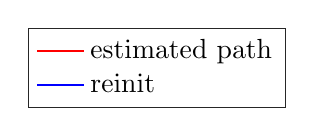
\begin{tikzpicture}

\begin{axis}[%
width=0.951\figurewidth,
height=\figureheight,
at={(0\figurewidth,0\figureheight)},
scale only axis,
xmin=-478.450911775336,
xmax=568.909731881523,
ymin=-17.6049100000001,
ymax=666.925859136316,
axis background/.style={fill=white},
legend style={legend cell align=left, align=left, draw=white!15!black}
]
\addplot [color=red, forget plot]
  table[row sep=crcr]{%
-0.0254918464850879	1.53029535298812\\
-0.0249375910222026	1.94734709129116\\
-0.0603236978857134	2.6546735108884\\
-0.0898810439677802	3.26129873758476\\
-0.122075910018214	3.77863002775995\\
-0.159570842980351	5.84214038823406\\
-0.162924757869628	7.08369056436346\\
-0.345776789656578	7.86663308840249\\
-0.274915939891177	8.64211113562301\\
-0.309598017917685	9.85377995390351\\
-0.277110670012233	10.8074353831107\\
-0.341823185024733	11.5749687633776\\
-0.217611982003351	12.8917266019904\\
-0.0592982609196149	14.535514156623\\
-0.180911942853752	15.86511539354\\
-0.297283259467498	17.8330042136393\\
-0.412075349790875	18.7361261341307\\
-0.45753291768454	19.5761622770474\\
-0.621156244022164	21.0674957763717\\
-0.980582354759486	22.4156368973729\\
-1.22745431999006	23.3028125720513\\
-1.40193957398277	23.7818677316401\\
-1.38814570798518	24.5045203072225\\
-2.27234059909732	27.090103133502\\
-1.99698008172313	26.599750220032\\
-2.10641148550549	28.5968708583948\\
-2.12832973202378	29.6371062106194\\
-2.17598796424889	30.7154871324073\\
-2.30067910404206	31.5854378822055\\
-2.45907796101916	32.0676868513679\\
-2.26907274159396	33.2344722663552\\
-2.44965781029554	33.7434621335118\\
-2.42633183226451	34.6703442074949\\
-2.26409672249432	35.6885730821861\\
-2.02200928137002	36.5560861882562\\
-2.11464297706809	38.5918738055132\\
-2.2790780780565	39.4298450322844\\
-2.33079259738496	40.5287786428546\\
-2.32348621152773	41.5347821989161\\
-2.61598248038879	42.9586032086692\\
-2.75390878914562	44.0874338224844\\
-2.84260537357017	44.6619622034007\\
-2.73393327844234	45.9088003321661\\
-2.72233550589239	47.0140262009282\\
-2.92329815798034	47.5907737467369\\
-3.1114129165952	49.5669407968523\\
-3.10749634212382	50.5822034293428\\
-3.2500223244702	51.5595653251282\\
-3.19057416753949	52.5993516136576\\
-3.42487733945348	52.7185018679645\\
-3.86473729462139	53.9467192635029\\
-3.82192343799324	55.2004471131418\\
-3.72844310151678	56.2768579050202\\
-3.87874198922826	56.5540555547952\\
-4.31576433504916	57.5131929181247\\
-4.50095451396497	59.3869146094641\\
-4.5574996462812	60.4392404725805\\
-4.55963752163573	60.676702682711\\
-4.32228998523037	61.2488392046191\\
-4.87131366603738	62.0681008052721\\
-4.97963140668309	62.8391231102824\\
-4.88007482342246	63.3552485041452\\
-5.05335190374172	63.8349645664496\\
-5.20937834338744	64.5954949838784\\
-5.37590875315335	65.1868099863566\\
-5.52549870207429	67.2202203170075\\
-5.49230224392353	68.1471525923533\\
-5.90059756790629	69.5266121775069\\
-5.94224632939223	70.1528542484596\\
-5.83067790095532	71.0105183601849\\
-6.23881006232067	72.1070665824533\\
-6.20102873297526	72.7757141401353\\
-6.04729823385154	73.6900879227054\\
-6.83730383226794	74.5136822411207\\
-6.79122267715735	75.4724191019868\\
-6.91877687145188	77.3406785323466\\
-7.22812021698276	78.4365832881394\\
-6.95072516286984	79.2980945101407\\
-7.33844971913853	80.0793778613153\\
-7.4014329956767	80.4294290986753\\
-7.99373625691982	81.4774066575055\\
-7.86605802354238	81.9059934294752\\
-7.77172752574243	82.4773062928979\\
-7.75255225554923	82.9982263260112\\
-7.73536254115288	83.7274702704368\\
-7.43530789685198	85.5881237523651\\
-7.26522876759875	86.7094611899334\\
-6.95474804758906	87.4861671355073\\
-6.52945786481193	88.2006488121833\\
-6.29331144174462	89.0440087794648\\
-5.6473003463594	90.1301212252086\\
-5.04471442850648	91.3758304114108\\
-4.79497511925477	91.4565841951169\\
-4.11366424911469	92.2814105611788\\
-3.29233119919528	93.240709055785\\
-2.06102851921597	94.2645452524725\\
-1.93117670430295	94.3598928400182\\
-0.250621775612316	95.3354218702807\\
0.797429792558788	95.7957750552428\\
1.78314953648874	96.1467649289709\\
2.88460614599643	96.509761291005\\
2.22574858995371	96.8430923732357\\
3.27687528932782	97.242501252346\\
5.17891322793282	97.5802344273431\\
6.1681268687833	97.8402884928389\\
7.24003034024114	98.1978908460427\\
7.59219028240269	98.1269917137799\\
8.5105584513945	98.2840030912233\\
8.66893008900028	97.9307079806763\\
9.59412183556174	98.2135026828747\\
10.1481630139105	98.2809483795584\\
9.98083027978335	98.1162695695153\\
10.2515634283344	98.2452558793527\\
12.4128066428538	98.4127634188667\\
13.2011844022571	98.1671672109638\\
14.5245082066301	98.3641225583476\\
15.7963695762376	98.5592167041786\\
14.9764319720182	98.3723096474683\\
15.8360033874039	98.186201278745\\
16.4323418296998	98.2484181765867\\
16.8010193333059	98.0835161469236\\
17.7133099208486	98.5353598195702\\
18.0022153354009	98.4012657457226\\
20.0130451999776	98.2675817807078\\
21.0712455696621	98.4241711260259\\
22.2034340671795	98.4101845003551\\
23.4639503534913	98.6275255517201\\
24.5937622194502	98.3200210698915\\
25.9356064401009	98.4580006219802\\
27.3709881514104	98.7834165356174\\
28.0022394924075	98.5724272238877\\
29.9094080381373	98.7902784237861\\
30.1626199572851	98.6195174419399\\
32.1989251843405	98.6858112080576\\
32.9521275332324	98.4219799985887\\
34.2351711456283	98.5100290841369\\
35.3513910150143	98.6232056950374\\
36.3166105089314	98.672217661454\\
38.1631441207067	98.8382969561731\\
39.1711719733013	98.9055763010074\\
39.6818056588983	98.6579558423154\\
40.9039613216276	98.7827938161883\\
42.2264589507336	98.783510597812\\
44.213758443799	98.7288557231846\\
45.2062298317859	98.7055711251752\\
46.4722095151188	98.7203559657082\\
48.326976830626	98.7257251565771\\
48.5642867029227	98.6527478169369\\
48.7294911339048	98.3930755001878\\
50.1424140534191	98.4110326394113\\
50.7015511333802	98.3398554972122\\
51.8494279869198	98.2799457623076\\
52.5303959166514	98.2516376449155\\
53.3425900382002	98.1888795231586\\
54.6623157384436	97.9657548563737\\
54.8482475388705	97.8567569243236\\
55.2244143633886	97.8833500919266\\
55.8384421447742	97.6760451068234\\
56.0395452800668	97.7829824360309\\
57.1340783897218	97.7966314998207\\
57.6666036854908	97.6510043901735\\
58.2211103989543	97.7231965890034\\
58.7301073817857	97.5682905210799\\
60.385515934906	97.1107229257761\\
60.9761692208895	97.0262569828221\\
61.4422364279443	96.9600004707297\\
61.923078776279	96.8903014774201\\
62.5444478465747	96.7684918488444\\
62.9898387027103	96.7375515446016\\
63.3117872413287	96.6937515846573\\
63.7954676193833	96.666744864621\\
64.4219313888184	96.7010659133751\\
64.855578720381	96.6610326248342\\
66.9636536857303	96.6368879330185\\
67.9284466315696	96.5671414670845\\
68.6136393023327	96.7170893713881\\
69.7152692247355	96.9504440438915\\
70.5552767279382	96.9350570007456\\
71.7554556588079	97.1821911451001\\
72.7301083374811	97.6547139584158\\
73.8347808202985	97.7783011536824\\
75.5725869240445	98.5904170675549\\
76.2378721606155	99.3003156352075\\
76.8641427168823	99.940431048246\\
77.7230885188133	100.452039672385\\
78.6836229239394	101.413173251268\\
79.2770662329756	102.367266712343\\
79.7470904119973	103.365994583476\\
79.9092157201661	103.271783381028\\
80.1743733697982	104.246060908402\\
80.4778337881829	105.513059163322\\
80.5993198952171	105.856753238037\\
80.5498945780941	106.345726418219\\
80.8863916947803	107.727219932189\\
81.6114269600833	109.624825750289\\
81.9586319675024	110.4917873926\\
82.4564643017161	111.101587418258\\
82.762803307285	112.45615926001\\
83.0922723831169	113.301516651837\\
83.4149313200726	114.167357888581\\
83.7058508282989	115.811771707526\\
83.7624692637908	116.94562175444\\
83.9126457684604	117.169408261462\\
84.3007461583004	117.833343127486\\
84.2819928033544	118.611686179488\\
84.146826424407	118.636767821165\\
84.3845624638485	119.016283810737\\
84.8621405152424	121.293685990612\\
84.9966925176513	121.327932985746\\
85.2240819588164	122.248220156345\\
85.4155342253503	122.808561364835\\
85.719858120791	123.782817470398\\
85.8826054115217	124.500745851405\\
86.0492378797153	125.458387885968\\
86.3251581690662	126.301440543795\\
86.3937188539614	126.990566358145\\
86.8912542641345	127.464673153117\\
87.3677830245447	129.317839382444\\
87.567211723829	129.877400274554\\
87.9651235568249	130.747323376724\\
88.0555008852286	131.201746095942\\
88.3200846916169	132.022585981679\\
88.5146892511074	132.799669186885\\
88.6358928035994	133.792372662622\\
88.9131465676964	134.224141256876\\
89.096136399828	134.755943535985\\
89.3085940272725	135.717965109684\\
89.8153123218939	137.551448607232\\
90.1235877873158	138.512304228395\\
90.4697960797617	139.078388276745\\
90.6920516923823	139.998023741152\\
90.8625781582068	141.464968746062\\
91.1376620400182	141.912331758265\\
91.3649394355048	142.364699216092\\
91.6236085242591	143.443091519136\\
91.962096284175	144.425925996681\\
92.1836757658171	144.957812358979\\
92.6494218541832	147.128225873418\\
92.8274668415432	147.947000321572\\
93.043327511792	148.64038383782\\
93.1825389694766	149.417940212159\\
93.3134009925863	150.156625858127\\
93.5920599236058	150.871654824285\\
93.3561782259374	151.846365880853\\
94.0062444197677	152.522141421041\\
94.0946224987294	153.193999489743\\
94.394980984906	154.0285499023\\
94.9506250382432	156.139511378517\\
95.2501238047098	157.276589817884\\
95.6745822378703	158.299881836949\\
96.119659865672	158.96189130575\\
96.9254791668891	160.89468461479\\
96.5103088393586	161.34289105974\\
96.8035646852944	161.730763515155\\
97.2004032203503	162.672901361198\\
96.9186425475122	163.351837557968\\
97.5337229353672	164.307707762183\\
97.7960602875196	166.202366291152\\
97.9992896289086	166.997300131022\\
98.1007170999768	167.929532950069\\
98.2536524286836	168.863580745745\\
98.4898346952099	169.904366379785\\
98.4484102522164	171.013251058507\\
98.2352650918821	172.088738897517\\
98.5079353406105	172.209711169409\\
98.8977008432825	173.049309290563\\
98.8294540756557	173.942349237048\\
99.0282082429124	175.917138556805\\
99.1455510243676	176.790238949825\\
99.1108313460639	177.806373350729\\
99.1227572762299	178.976050201156\\
99.1410726154717	179.714001263582\\
99.3834306397597	180.048450874798\\
99.336642171872	180.895294825533\\
99.3502256670279	181.718104793466\\
99.3337235671963	182.22689780013\\
99.4545121928192	182.96599948506\\
99.5018465402586	185.006374111549\\
99.5729657532157	185.795220648459\\
99.3970972250681	187.068736166692\\
99.544081235651	187.660136707246\\
99.6328255615419	188.74019608955\\
99.279127659447	189.748583894515\\
99.1548891827147	190.6654931326\\
99.2370956924192	191.439547695707\\
99.2267739633768	193.42836665194\\
99.1923413001119	194.418269815055\\
99.062389315362	195.375506546448\\
99.2289351917725	195.687437803877\\
99.0994222641157	196.939886983181\\
98.7654125932142	198.035735503403\\
98.9536040769641	198.756071448753\\
98.9246005258224	200.705147856396\\
98.8874384000429	201.643821271399\\
98.9205250479406	202.498842882555\\
98.7135064667041	203.609851731272\\
98.5827465763417	204.853825625594\\
98.9500115110317	206.622710999797\\
98.6975040826304	207.470966741501\\
98.7668297077694	208.81569102341\\
98.2518368010219	211.440199517968\\
98.1770712815493	212.531467161141\\
98.1199771802931	214.419988621423\\
98.0825830280071	215.386879436705\\
98.1153738475582	216.128148360135\\
98.2086192702682	216.801668050291\\
98.0163462813238	217.957970819439\\
97.9827007092966	218.751449428795\\
98.0626361749252	219.696747024466\\
97.8580178409277	220.666062917953\\
97.7657284624476	222.705837705202\\
97.781761973794	223.715870461332\\
97.7568550296704	224.81690953634\\
97.7093324908031	225.826851650268\\
97.753462715551	226.60002483732\\
97.899727764187	227.371139413321\\
97.7529393388261	228.166476973698\\
97.4798298247375	228.941172103432\\
97.2321818508004	229.766237241626\\
97.3351840892595	230.456063665679\\
97.3144960725607	232.460474594581\\
97.2897549029264	233.433511723224\\
97.3079634081385	234.357641324376\\
97.2031022856822	235.40254592779\\
97.3286940206772	236.274442738623\\
97.3733832439296	237.361190170033\\
97.4893152207055	238.547985570722\\
97.0691991064325	239.124484396409\\
97.0091973525259	240.289982647587\\
97.1304327305043	241.298753792839\\
97.1877782703995	243.189625930062\\
97.1876187726158	244.107342110627\\
97.2740925981774	245.063371286114\\
97.4172397020602	245.935391579889\\
97.428546063039	246.87753673821\\
97.2357533818536	247.640868082904\\
97.317457302081	248.950058293701\\
97.1602140496479	249.042282495506\\
97.4487016122657	250.58102379216\\
97.4463293136912	251.802849600725\\
97.3636797727139	253.856310941121\\
97.3901645657072	254.925762505496\\
97.2385578570516	256.105547871531\\
97.3621165587876	256.978644601477\\
97.2975167205967	257.765053754391\\
97.2418856773053	258.815428258919\\
97.1516476275366	259.708646694917\\
97.2071947641934	260.681607058821\\
96.7011698314686	262.667162629578\\
96.7229982976873	263.154823797727\\
96.7427775277447	265.139166402239\\
96.4480827835196	266.29614193386\\
96.5063228522242	266.9018702535\\
96.502511038	267.920281328143\\
96.2380527554972	268.941133039757\\
95.8676875184674	269.724843333998\\
95.6200085305505	269.749783394892\\
95.2638721809408	271.553580141357\\
95.5288750955712	272.837479500114\\
95.6677371564531	271.667571117989\\
95.7743878161895	273.574219659123\\
95.6327278924485	274.656945925954\\
95.6526736388049	275.035202492088\\
95.5800060480144	275.040833283391\\
95.4965798726979	275.194867286143\\
95.2895238470901	275.592199699495\\
95.3834050339676	275.745160420186\\
95.3233243115685	275.971047760802\\
95.2316476849159	276.194703108601\\
95.2272775052936	276.30892186746\\
94.4228741645387	276.633757786361\\
94.2042572075126	277.653653795025\\
94.0920506323983	277.699074509446\\
93.7292996744809	278.052931649746\\
93.6092689126441	278.504802998374\\
93.3153071711114	278.678159126385\\
93.0511915685003	279.009285433382\\
92.7514107810436	279.129916492549\\
92.5175108097781	279.44385946719\\
92.2142567898704	279.820908115431\\
91.0281926828235	280.437599095476\\
91.0310785347896	280.476545212659\\
90.7077921567882	280.575156126495\\
90.2973830124053	280.986507006175\\
90.2647765418932	280.850716699237\\
90.3213557484851	280.874590601117\\
90.3889807173694	280.873150682221\\
90.2827392588201	280.873427691616\\
90.0374777875742	280.946594168375\\
89.9767825472452	280.97292329174\\
87.8390643131039	281.121769499472\\
86.7758073388856	281.216914701424\\
85.6544301933939	281.31332803805\\
84.5995674087014	281.184205960077\\
83.6508580216933	281.386561979885\\
82.2251061282914	281.590063202275\\
81.3625966777724	281.785685174432\\
80.3088189020232	281.199800598554\\
78.877220243863	281.920311898614\\
77.5991839087184	281.815957546827\\
75.592051116952	281.862043618773\\
74.6351924709613	282.053699576232\\
73.4984455214727	281.994340510114\\
72.0479124855079	282.031237460481\\
71.0048618297533	282.036561438413\\
69.6677028075266	282.046357492773\\
68.3324969988874	282.45024186922\\
67.8692443916789	282.675242819926\\
66.2872058882843	282.758938845338\\
65.1669385879937	282.863986608207\\
63.2134334547598	283.088520433892\\
62.0090160030093	283.092262736309\\
61.4356692266479	283.020026023908\\
60.6819599027938	283.112751483224\\
60.0299688857487	283.092587145309\\
59.1321361106731	283.112703905307\\
58.2534275938114	283.195456559683\\
57.2770637866808	283.329105826634\\
56.567624389357	283.001671283967\\
55.1597183659055	283.356537026635\\
53.7171374180246	283.423924070062\\
52.7832207388181	283.639905503139\\
52.0467357003402	283.657912965716\\
51.493045115607	283.714920173091\\
50.6503112573758	283.947681944612\\
49.7742561240248	284.09579685291\\
49.2292694512978	284.163106325583\\
48.6630878537546	284.179769924374\\
47.9866603425618	284.259090689275\\
47.3230767689064	284.352427286795\\
45.2151111044766	284.369330582576\\
44.2585914220981	284.448700905124\\
43.1125912960108	284.663512039087\\
42.2716065325503	284.719331294265\\
41.4181069071546	284.612485537442\\
40.297707413537	284.816651311679\\
39.4671180289811	284.837850992241\\
38.8353457466918	284.72862303274\\
37.9430551876562	284.651834948126\\
37.4048491896148	284.536549583384\\
35.4883199608337	284.647080888081\\
34.3469720163117	284.421557301444\\
34.0272986042716	284.409054047117\\
33.3029985283589	284.642001311766\\
32.3821021304997	284.850748611215\\
31.1750867906643	284.374697214561\\
30.8832708044295	284.592595374352\\
29.913764077224	284.442431573567\\
28.0341072777321	284.475538701518\\
27.3036779732485	284.373380793545\\
26.3412663145812	284.529803840323\\
25.5979787546491	284.497308662393\\
24.9418804640711	284.552651805808\\
24.2637138677878	284.179125678909\\
23.7866652432886	284.235688093077\\
23.163067572468	284.333383743824\\
22.251429786829	284.377507487762\\
21.5219927415144	284.762116265869\\
19.5116767426004	284.870560657594\\
18.7073739040291	285.066816864159\\
17.6973446506764	284.854847513677\\
16.7492678608288	285.30632961818\\
15.9795051176022	284.99286602644\\
14.8610910858699	285.164676775751\\
13.8861356145606	285.163971708539\\
13.3291048653386	285.339325878951\\
12.6388139074277	284.562614992046\\
12.1679523643265	285.366564091498\\
10.2714660802827	285.551873739589\\
9.44071985073852	285.82334700803\\
8.64558573633682	285.711302684951\\
7.99031641136685	286.384411523437\\
7.33731795542608	286.055686262888\\
6.82486909902222	286.364774871972\\
6.6179832542079	286.66860525883\\
6.21398396486262	287.030179815892\\
5.44366888314555	287.049820740183\\
5.27386388465087	287.015354020159\\
4.89311064659625	286.680627527626\\
4.89414842818961	286.660127078987\\
4.88658994749166	286.657835251561\\
4.91551589782707	286.616758431272\\
4.91975202794841	286.604552531756\\
4.90026464466442	286.614395620684\\
4.87621017748187	286.631470523108\\
4.88576428317739	286.628104063645\\
4.87461452693026	286.636910802733\\
4.86968101561024	286.629842030507\\
5.81780462698408	286.245634180133\\
5.63866380250233	286.131341575055\\
5.81166977992147	286.177855949059\\
5.03697254845152	286.262998392181\\
5.4742378429069	286.244900702191\\
6.8547843334764	285.868414587869\\
12.1243990127677	286.511270742009\\
8.32694452159818	288.294675793508\\
-1.09413320029126	293.916756072537\\
-21.6474812698809	297.708458705245\\
-21.9325898235476	297.117936075686\\
-21.9956942627265	297.193070382587\\
-22.4139303044929	297.503493830077\\
-22.642948207287	297.298906773929\\
-23.7130104981462	297.421027054268\\
-24.8740118107549	296.164993373517\\
-22.0996577749431	284.098947578509\\
-24.3952243957361	284.410182869828\\
-26.7894106957737	282.774466563181\\
-31.2975511221051	282.003256724141\\
-32.2935675809144	281.877093047675\\
-32.6407809351338	281.918013230164\\
-32.7288945605468	282.066775973329\\
-33.0600208955712	282.153448745147\\
-33.448140572418	282.381023392334\\
-33.9071052802694	282.450007419116\\
-34.1990461757951	282.68196191464\\
-34.6299354525934	282.752920451045\\
-34.8552647871615	282.974991294802\\
-35.0631308132814	283.093610320396\\
-36.7905156728052	284.140652561951\\
-37.8517777485731	284.536418990438\\
-38.240915042885	284.980480163258\\
-38.5308275032632	285.596561274632\\
-39.1761023590381	286.134903624664\\
-39.2277011507638	286.755810325358\\
-39.8792712738083	287.280771538393\\
-40.278429915754	288.00736956512\\
-40.3790667761522	288.656719489577\\
-41.1803147855581	290.122720796797\\
-41.7399874065361	292.002006064696\\
-41.9907459333768	293.052639890348\\
-42.2365706994355	293.94841923912\\
-42.584739817209	295.238080086862\\
-42.7656262174163	296.256636948109\\
-42.8992548653958	297.623882847864\\
-42.9792990748003	297.946769303611\\
-43.5500921043224	298.961793561077\\
-43.7747171220709	299.690160217623\\
-43.9739644521407	300.027422888397\\
-43.598580244308	301.941545688292\\
-43.7136070800627	303.517465846708\\
-43.5108105096143	303.346115788725\\
-43.7489805383992	304.803408257338\\
-43.8317762280053	305.324464349615\\
-43.7299668219603	305.455979629804\\
-43.2871727653318	306.180594854728\\
-43.5087620789777	307.353117095163\\
-43.3252112845172	308.030803691621\\
-43.5513207554295	309.450791733653\\
-43.1763267634572	311.577270301302\\
-43.2235498047363	312.147778542548\\
-43.2393829074008	312.835002915232\\
-43.1882848291291	313.769277571182\\
-43.2962491857431	314.329877586784\\
-43.0417766873351	315.033251461994\\
-43.1358604130653	315.392439470541\\
-43.1429525535945	316.192657760085\\
-43.1255267149717	316.666268957715\\
-43.0632112562022	316.884758755732\\
-42.7503120039844	318.932326146461\\
-42.4270312043061	319.759683048941\\
-42.3113763096504	320.781291576106\\
-41.9969587322797	321.870434473599\\
-41.9973113021666	323.809834226097\\
-41.6371299633755	324.807994882835\\
-41.7981519180195	324.733029444512\\
-41.7856129620457	324.790193963044\\
-41.7489244505678	325.89590148042\\
-41.6374978657894	326.232867717162\\
-41.2620773298299	328.124309112912\\
-40.9936678966992	329.177202596928\\
-40.8610303275784	330.099674329465\\
-41.5356815853264	330.595249741425\\
-41.4611636776108	331.227394235996\\
-41.6183322482453	332.29545209413\\
-41.7869089749057	332.544173505866\\
-41.9777301250788	332.858330472165\\
-41.9981185840822	333.882669258739\\
-42.1439448798533	334.499610876784\\
-41.5646257820287	336.391326709811\\
-41.2003618916538	337.361164210756\\
-40.6581523651115	338.905478209979\\
-40.5057677661375	339.813774661806\\
-40.1767298099489	340.511864706968\\
-39.997173223703	341.326950326718\\
-39.4462685562649	342.646044706824\\
-39.2065597329264	343.386042689822\\
-39.6753259906417	343.116588814099\\
-39.4076465660695	343.861347913106\\
-38.80671789743	345.731039029314\\
-38.5130514941361	346.585117910823\\
-38.2857849081704	347.514298053445\\
-37.8841874239085	348.532247759923\\
-37.4597696255134	349.762765361236\\
-37.0533754550049	350.70407850718\\
-37.0104694006025	351.281937348237\\
-36.3860566173734	352.610009043194\\
-36.4150768439415	353.138417862204\\
-35.8584692409962	354.094548514959\\
-35.190246470062	355.970950703738\\
-34.7182170414074	356.80638666928\\
-34.1327174124296	358.638866472817\\
-33.8323306566339	359.294747967461\\
-33.5113346937311	360.209030571828\\
-33.0738854532705	360.934896011096\\
-32.7568961617703	362.057551189245\\
-32.4255717816118	362.825168711271\\
-32.2301931917986	363.926347508694\\
-31.9125337705905	364.692664499014\\
-31.427241105816	365.831351934691\\
-30.9856987021938	366.58770609911\\
-30.3919839444071	368.508131764299\\
-30.0738454540652	369.496509660904\\
-29.8545098548981	370.16041020134\\
-29.5145001927676	371.101017144499\\
-29.3064404769259	371.925100129337\\
-28.5003762026391	372.936526668802\\
-27.8514047851803	374.047847575465\\
-26.8745203891184	375.422651789382\\
-26.4045560900486	376.196767730858\\
-26.0938826170801	376.536763741913\\
-25.7606662340508	378.556275004992\\
-25.5443134593624	379.406629878231\\
-25.3306833842212	380.433799663233\\
-25.0480514184196	380.99110142449\\
-24.6390802102253	382.076805594361\\
-24.6409750791932	383.300991966794\\
-24.8255099311086	384.238165557673\\
-24.4531417750676	385.152025704709\\
-24.3180657938585	386.121825754955\\
-24.3643735546848	387.161568165843\\
-24.0074106343	389.057451276827\\
-23.8468597954946	390.038357582657\\
-23.7958510179256	391.006786867751\\
-23.5505971078725	392.090376742379\\
-23.6145438463765	392.931431999113\\
-23.3281701857092	393.868187953662\\
-23.4785119203719	394.508074415702\\
-23.0796963818055	395.273784218602\\
-23.178568123108	395.936678648487\\
-22.9645897298312	396.993294126907\\
-22.5260638884999	398.856758196578\\
-22.2561773540322	399.89388334255\\
-22.1689194094002	400.75361057385\\
-22.3825879144507	401.558034028442\\
-21.7923320457677	402.583478566175\\
-21.9629482167302	403.157477905221\\
-21.9242766293188	404.104253414177\\
-21.557515844212	404.967015487928\\
-21.6107172418382	405.772548290998\\
-21.3164250832139	406.345063304013\\
-20.9551906691708	408.218652168773\\
-21.0030776280658	409.184658382844\\
-20.8498996214261	410.100406636337\\
-20.807848580165	410.807991230701\\
-20.9947440910597	411.741671153775\\
-21.2218084243845	412.804401675641\\
-21.2699329898167	413.734845478609\\
-20.8633732608419	414.730859570341\\
-21.2087976793107	415.520675909405\\
-21.3614407834967	416.132081958422\\
-21.8842160478211	417.948962953001\\
-22.0323693577784	418.502191327571\\
-21.789416607025	419.011793724359\\
-21.7012760556811	418.34239895617\\
-21.7566022495132	418.14314853426\\
-21.8589756972023	417.874382814643\\
-21.6327124654056	417.326322855613\\
-21.5982017906372	417.123864775533\\
-22.6062106933622	418.067050014456\\
-23.2989366507926	418.759823283767\\
-24.4808180210422	419.45911805305\\
-25.4492168539001	420.020506903419\\
-26.0555134369592	420.660759086592\\
-26.9880492235558	421.782176916216\\
-28.932239460789	422.401995603816\\
-29.1054551137119	422.071182431233\\
-30.3006473964457	422.67450468789\\
-31.6379738980682	423.399855272451\\
-32.6546547677045	423.79929205372\\
-34.1409170145935	423.325613622328\\
-36.0140309669621	423.195747721855\\
-36.8040631478539	423.372614663329\\
-38.7191231622829	423.629689236321\\
-39.4573651504033	423.667380607129\\
-40.6919470225948	423.69131276039\\
-41.6501744319605	423.972105668339\\
-43.5023945303334	423.761928255547\\
-44.5172606541073	424.198392051902\\
-47.0786337301568	425.008698510216\\
-48.4382607087992	425.329750812905\\
-49.1815975753576	425.643689585481\\
-50.3044940758423	425.596992725439\\
-52.1190273803989	425.508087034689\\
-53.3739975484041	425.838516282859\\
-54.3854504488481	425.947786513815\\
-55.2662359613265	426.033096004898\\
-57.1570997470184	426.106601668627\\
-54.9261321831312	426.005680165437\\
-56.5454660895693	426.100549514163\\
-56.3956245107714	426.31077763637\\
-55.8843748743304	426.148953569316\\
-57.7465842341457	426.465810578737\\
-58.540483006883	426.565894151189\\
-59.5455014763192	426.797207082731\\
-60.27106376592	426.918312276247\\
-61.0874844614485	427.131797086244\\
-61.8104343472718	427.378911022402\\
-62.4924918533574	427.407736288477\\
-63.663771374348	427.573483301906\\
-64.3684298831362	427.737145161782\\
-65.194943739647	427.795164032515\\
-66.8569703185152	427.997099516283\\
-67.9416514948348	428.075667787475\\
-68.5559515899555	428.224591336317\\
-69.4784209210848	428.184835252725\\
-70.0940890103205	428.473226815816\\
-70.7564010617623	428.48620357468\\
-72.8000776185079	428.765806976616\\
-73.7651624161099	428.812675109012\\
-74.6160215447673	428.93928505712\\
-75.6186125792385	429.014125254906\\
-76.9860063201794	429.567967107673\\
-77.8530517362815	429.971965251684\\
-79.3834791457658	430.063634872338\\
-81.1735288751672	430.800836037772\\
-81.2345857163772	430.338029200818\\
-83.1153900704311	430.533574853672\\
-84.8002106491713	430.870734188082\\
-85.1645951966345	430.898565315034\\
-85.8471407148557	431.046890871356\\
-86.765940535305	431.610272649025\\
-87.3433026952954	431.659609262165\\
-87.781766963224	431.626490266378\\
-88.5018224013614	431.956047508639\\
-89.2058900398045	432.287360456399\\
-89.7464448466527	432.264338826852\\
-90.1207844877668	432.427330901655\\
-91.7141806133781	432.756222331805\\
-92.5071705635437	433.025419559436\\
-93.3024199519724	433.043197346022\\
-93.9089274215956	433.335212385403\\
-94.5244208156455	433.435688505955\\
-95.1401746679506	433.49346482149\\
-95.8962509775628	433.543800053336\\
-96.4527939499195	433.695999795514\\
-96.9588174190874	433.9270651879\\
-97.7160691662457	433.859016446358\\
-99.6298884530059	434.035184008532\\
-100.349573429023	434.298706120222\\
-101.098053542803	434.472520615438\\
-102.116077625647	434.543907749256\\
-102.756779559106	434.748273994604\\
-103.428717962516	435.439762520866\\
-103.489455262586	435.103100832187\\
-104.272737116368	435.304442652646\\
-104.994600874518	435.542865024617\\
-105.422297147173	435.467499182063\\
-107.406582379164	435.504439311781\\
-108.284231588299	435.718472744823\\
-109.19305801003	435.794513682104\\
-110.354093163749	435.747533836552\\
-111.230112520716	436.07459513435\\
-112.108912370377	435.947305636096\\
-112.922920793648	435.871310424858\\
-114.528908801378	436.113977206586\\
-114.649251162082	436.273406047359\\
-116.983945265319	438.206339846062\\
-118.993465581575	438.383664768856\\
-120.17717796134	438.305639782493\\
-121.127818321715	438.35758246247\\
-122.698122478298	438.836971262632\\
-124.175551391527	439.307113855348\\
-124.483245312582	440.018166695881\\
-126.029226733273	440.07475627734\\
-126.414903513413	440.816622850513\\
-127.046395592027	441.201306097447\\
-128.175384072724	441.577741206979\\
-129.831452633958	441.516382690121\\
-130.850521067343	441.553474535537\\
-131.980648375894	441.638761961752\\
-133.314049980227	442.213364839973\\
-134.107846371861	441.573593727452\\
-135.398420734056	442.000838556606\\
-136.400357175879	442.133034480093\\
-137.250683642937	442.339113987724\\
-138.592583697254	442.494430397981\\
-139.620513281261	442.627003644589\\
-141.511295360663	442.701110846743\\
-142.436354281271	442.846522180456\\
-143.200763038882	442.728436248776\\
-144.163343777678	443.062699837284\\
-145.001639102289	443.169852648834\\
-145.965972092768	443.419952425293\\
-146.568462105135	443.522095671828\\
-147.462445820775	443.508464795417\\
-148.507232128216	443.843028647461\\
-149.443914413773	443.976009106532\\
-151.51963973449	444.096025078129\\
-151.875589951886	444.157910406988\\
-152.714495885772	444.315636676042\\
-153.672702124216	444.472174920355\\
-154.066073938352	444.677987881372\\
-154.830804435742	444.697499389072\\
-155.559230189152	444.858956807841\\
-156.275121136863	445.068688737813\\
-158.00710935904	444.826909377607\\
-159.914725443068	444.706551115892\\
-161.565839315621	444.553701702634\\
-162.271714053477	444.560761664545\\
-163.117025599184	444.444726743732\\
-163.252220532387	444.271075194074\\
-165.137442770615	444.569888391836\\
-164.988234587647	443.747763388013\\
-166.281872070626	443.98277381405\\
-166.858134253344	443.718515212447\\
-169.153461548866	443.35699285489\\
-170.255266150194	443.117839339026\\
-171.064990278573	442.918514603147\\
-172.24047608771	442.978893794973\\
-173.26184180551	442.956424940468\\
-173.614869110604	443.158797493978\\
-174.625740535327	443.03247108221\\
-175.547159557266	442.46310213636\\
-176.68833423064	441.989850643207\\
-176.807399247738	442.167599677951\\
-178.745014157082	441.940660185948\\
-179.673809461521	441.809736894797\\
-180.560409959321	441.685053459949\\
-181.535859853744	441.652248741714\\
-182.206403966032	440.586161196037\\
-182.928308036858	440.662831928689\\
-183.919788538044	440.630118787024\\
-184.405398667366	441.161208001045\\
-185.207082543935	441.443500964639\\
-187.100373850434	441.193839645593\\
-187.788838591914	440.911756877784\\
-188.660656197463	440.710268824822\\
-189.60496908015	440.726650171052\\
-190.142112405432	440.531358831784\\
-191.047736102829	440.240509627416\\
-191.410935554252	440.644244393227\\
-192.234471305681	440.157022587354\\
-192.992089684225	441.024416569025\\
-193.353238251407	441.040512446334\\
-195.23441514025	440.457436308333\\
-196.015609947835	439.979995168434\\
-196.71805025848	439.740609384709\\
-197.911689144837	439.252739941214\\
-198.598620103861	438.865850110661\\
-199.393565571607	438.136305256211\\
-199.919420287917	437.801991064321\\
-200.452771045643	436.900623589228\\
-201.029901556302	436.611348153979\\
-201.448028095958	435.916391943141\\
-202.419625417267	434.533391527104\\
-203.102022139242	433.629585246291\\
-203.737429133255	432.870322520585\\
-204.128146966817	431.79668270895\\
-204.299493677602	431.110651980566\\
-204.519217703514	430.120203011464\\
-204.888486441909	429.14082460371\\
-204.952617532679	428.060354492723\\
-205.068791181435	427.047353487512\\
-204.843966274641	426.526219673147\\
-204.883597481544	424.564255192547\\
-204.718007554966	423.441884761951\\
-204.640292762277	422.610526190823\\
-204.296285337692	422.0369292859\\
-204.503167396047	420.904657753657\\
-204.29544263376	420.263799728397\\
-204.282660577156	418.818337342755\\
-204.232976362549	418.171108830746\\
-204.205421483634	416.617747211783\\
-203.871740664308	414.674583227839\\
-203.783028741626	413.948640093203\\
-203.531103391066	412.738323755226\\
-203.461620617955	412.138759190845\\
-203.11749154115	410.247466287839\\
-202.890581308402	409.245829101122\\
-202.867433903518	408.410638351751\\
-202.898266338403	407.559165311175\\
-202.536426779754	405.812227214051\\
-202.311118722592	404.826067246706\\
-202.148581883533	403.819080423904\\
-201.939560150217	403.028754405161\\
-201.55012549705	401.174117690788\\
-201.33719644249	400.672553464751\\
-200.929613426139	399.152095535186\\
-200.71768464797	398.21778433385\\
-200.520817121942	396.262910792246\\
-200.248704266538	395.220110126337\\
-199.873400289354	394.235283776329\\
-199.69571367488	393.609664052164\\
-199.671642717824	392.315541052832\\
-199.648814491891	391.487970842894\\
-199.075493985983	390.487254659586\\
-198.983228571484	390.140188213049\\
-198.994802733178	388.997443040701\\
-198.761518306306	388.174067345444\\
-198.554041668995	386.443637715421\\
-198.500749832608	385.86099008101\\
-198.290810032591	384.936903406335\\
-198.15053993718	383.810790330223\\
-198.043491423291	382.38184822126\\
-198.04800030859	381.342208545427\\
-197.813865259851	380.219919115455\\
-197.774507977942	379.235201286617\\
-197.596211645138	377.974224466124\\
-197.367619826272	376.819186030558\\
-197.235753642877	375.526077670948\\
-196.950617989511	375.188031625862\\
-196.701425648398	373.215899179309\\
-196.517884360019	372.246941713418\\
-196.356191243257	371.225626214726\\
-196.365344620786	370.315842245074\\
-196.123980412217	369.210386533513\\
-196.012539332411	368.175262892963\\
-195.748216834899	367.288073689373\\
-195.714509674055	366.470880697325\\
-195.450962441443	365.518796180992\\
-195.32912834259	364.325721071044\\
-195.160724672006	362.519484854157\\
-194.883672720518	361.695933494079\\
-195.221971907468	360.793889795494\\
-194.89748399245	360.303268235448\\
-194.840139729922	359.678741214939\\
-194.722068893017	358.947450648899\\
-194.6742113085	358.756223734838\\
-194.515080966593	357.880862842214\\
-194.598190268089	357.235304352587\\
-194.388085687339	356.240108453043\\
-193.985596791364	354.471219183801\\
-193.922153630291	353.350747046341\\
-193.606935786994	352.599114199286\\
-193.318573824463	350.651958719438\\
-193.094860627384	349.665080173539\\
-192.874922698351	348.873449286006\\
-192.699149590552	347.883267668442\\
-192.841014806091	347.349350391667\\
-192.447404115819	346.167515122206\\
-192.551947354629	345.723599730507\\
-192.204525589519	344.550977531425\\
-192.076160861198	343.793029325174\\
-191.934631062874	342.766672267249\\
-191.440897227619	340.856651679621\\
-191.405114251341	339.885430734527\\
-191.408450927923	338.614719566227\\
-191.210202176759	337.648209625076\\
-191.0955450957	337.079576313726\\
-190.8104818106	335.801486739304\\
-190.759010075684	334.548154526338\\
-190.647142581882	332.921059387906\\
-190.381250495236	332.220253168823\\
-190.09764475493	331.355920820502\\
-189.599677686115	330.515356285576\\
-189.51626844727	330.476844248108\\
-189.47629011886	330.105331461686\\
-189.351081197991	329.4987340164\\
-189.046066423193	327.556350946723\\
-188.819459178215	326.55910648464\\
-188.671087466693	325.733193943475\\
-188.548964718481	324.730859744635\\
-188.249393201765	323.272200959535\\
-188.099383385199	322.289980674829\\
-187.952831439818	321.340227964422\\
-187.716651728809	320.783709052233\\
-187.569203058186	319.862943138419\\
-187.51933354047	319.089210129986\\
-187.411113724881	318.735447326202\\
-187.315216107465	317.580616852423\\
-187.245485553632	317.243014451929\\
-187.052892473039	317.368611720462\\
-186.724339550279	316.483779975671\\
-186.712742284816	316.366015666822\\
-186.374474654876	314.587048101908\\
-186.222741030376	313.707408165097\\
-186.328576050131	312.983494361384\\
-186.168877207738	312.33276013057\\
-186.0414891355	311.644740830998\\
-186.009739355011	311.33729066531\\
-185.662474875665	311.489842631413\\
-185.603972137993	311.015739319398\\
-185.60086046951	310.639793709774\\
-185.399880895628	308.709203521963\\
-185.108360528595	307.874768645202\\
-184.967940015174	307.046868416085\\
-184.749570046928	306.444552589234\\
-184.87580124872	306.476406813815\\
-184.832561453766	305.878549949369\\
-184.824915848063	305.577407566472\\
-184.777834140275	305.595689553982\\
-184.727702120915	305.752665259821\\
-184.787360281981	303.802450530486\\
-184.554426999288	303.350378913323\\
-184.553403525135	303.632822995282\\
-184.451089781549	303.732872107001\\
-184.432322877842	303.329187190376\\
-184.355776524176	302.752822885452\\
-184.230109041303	302.47788960925\\
-184.109369460495	302.29864976899\\
-184.038749085504	301.928744928664\\
-183.984279656125	301.610863410557\\
-183.319701989335	300.402375817618\\
-183.037279604349	299.818065833475\\
-182.70923559321	299.403389697598\\
-182.665049912993	299.256986249335\\
-182.441080808295	299.013327596251\\
-182.140433703693	298.812000844808\\
-182.115335081432	298.649470083603\\
-181.435732448587	297.842145712298\\
-181.987075288714	298.071907080616\\
-181.653106789532	297.247278618742\\
-180.053482058705	296.200438665857\\
-179.074826952868	295.659470246376\\
-178.205220670122	295.574215667038\\
-177.297026890306	295.163588314851\\
-176.330455805134	294.832636368504\\
-174.206381429618	294.136334398123\\
-174.303595830644	294.371278123911\\
-174.329574273759	294.488667641679\\
-173.056634236002	294.368441913304\\
-172.079963461044	294.505445056803\\
-170.039359834674	294.547851021997\\
-169.139973208246	294.567344156578\\
-168.128434278474	294.481253636504\\
-167.428006056359	294.614497308925\\
-167.211865352505	294.437761045598\\
-166.739801651971	294.526712244319\\
-165.36930133165	294.908668615417\\
-164.099579508988	295.052545184572\\
-164.397541246068	294.847932698736\\
-163.075853370532	294.966973176136\\
-160.988505334135	295.252797848909\\
-159.992106330424	295.449560057087\\
-158.852585991045	295.553631012804\\
-157.610224687394	295.532858046865\\
-156.33989452338	295.752526457233\\
-154.392908409661	296.324212961799\\
-153.655368525922	296.248340510647\\
-152.740963527511	296.473978180415\\
-151.614514975228	296.408380534155\\
-150.081733595501	296.903696690653\\
-148.087367114371	297.136266402496\\
-147.025027667026	297.174010104509\\
-146.180725902307	297.406610226916\\
-145.074294312549	297.517134665363\\
-143.918462676194	297.660204940467\\
-142.979687513341	297.875909206768\\
-141.956526820531	297.872648846878\\
-140.95055493493	298.067489762137\\
-140.1070734803	298.269382935246\\
-138.624820225905	298.503680263791\\
-136.448351322237	298.839426074967\\
-135.60282507989	299.009381665628\\
-134.332331322358	299.328759360714\\
-132.706765394383	299.685246521929\\
-131.930409494218	299.665369430564\\
-130.267002449755	300.186676129967\\
-129.475801642436	300.370104206535\\
-129.585168216126	300.245955121714\\
-129.38914120113	300.352973548849\\
-128.939527437394	300.488053409355\\
-127.38471671416	300.810272741203\\
-126.698180521934	301.022814965795\\
-125.900564632091	301.172062003643\\
-124.023688515995	301.447465547751\\
-123.095599451321	301.528020548548\\
-122.096788003167	301.83068889455\\
-121.495836799503	301.876119850052\\
-120.457836404579	302.13187495836\\
-119.870392579065	302.04452716488\\
-119.516894438966	302.10243620126\\
-118.584810419145	302.239977010405\\
-118.064220672299	302.308470661745\\
-117.357560552133	302.417754116002\\
-115.069933343456	302.795489505627\\
-114.207832652094	302.787414665838\\
-113.189117764908	302.916040579454\\
-111.963479759941	303.079069774467\\
-110.848347766221	303.33577015347\\
-110.413804908631	303.077782671404\\
-109.603634146568	303.082774769273\\
-109.146564206908	303.000588538572\\
-107.095980207844	303.102314442293\\
-105.80464536871	303.282016756706\\
-105.16017288623	303.404252034133\\
-104.183870354006	303.543768360332\\
-103.599326106614	303.392025237892\\
-103.204923857001	303.258565256223\\
-102.177675779219	303.365740322239\\
-101.838385721253	303.255511848036\\
-101.255267728024	303.106818543619\\
-100.948847877528	302.622894775335\\
-99.0179936337425	303.15043670293\\
-97.8027663527451	303.605896398131\\
-96.3837839929258	303.797489635118\\
-95.3157718676448	304.000952559397\\
-94.2459608246413	304.097984753672\\
-92.5267108898135	305.22515802157\\
-92.1248847665838	305.838947486759\\
-90.9805685567837	306.785746950532\\
-90.4687156915441	307.367924104001\\
-89.5262883691311	309.612933955729\\
-90.0002064247981	309.867868577157\\
-89.6403228285753	310.393445433112\\
-89.0356640770404	311.590255988741\\
-87.5210014752921	313.170084297937\\
-86.9683796675703	314.396723622612\\
-86.1457023384102	316.295269168042\\
-85.9712025864733	317.014826427376\\
-85.7511642660657	317.677350903023\\
-85.5410694881461	318.767844522778\\
-85.3898123131886	319.978153501168\\
-85.3998925926811	320.664930906584\\
-85.3498659582806	321.298868678206\\
-85.3236473072503	322.617409824788\\
-85.4445836743177	323.168803417302\\
-85.2812946212988	324.339169919973\\
-85.0118598848344	326.358021757455\\
-85.0459322602387	327.425487408493\\
-84.4981039707929	328.697385021544\\
-84.4830872824882	330.324764655081\\
-84.2063424403005	331.47585113919\\
-84.2459208646898	332.153656790049\\
-84.1307680556541	333.154872573521\\
-83.8622116043736	334.217257120704\\
-83.681200456067	335.02605013443\\
-83.4628083430067	336.583122574527\\
-83.0232964428922	338.244446657524\\
-82.4921697144465	339.01175050393\\
-82.3300153729474	339.679727791439\\
-81.8942854242555	340.558810628532\\
-81.5340355214961	341.631594146073\\
-81.273641516286	342.076736679865\\
-80.6312834293633	343.097692050735\\
-80.1021124394177	342.881010729591\\
-79.377628806178	344.261163456447\\
-78.6840099759652	345.418648544727\\
-76.8953881817485	346.578360376114\\
-75.8719618730628	347.243033032895\\
-74.9744385380533	347.657315698536\\
-74.2675126792882	348.170717767632\\
-73.7334604741285	347.834690216607\\
-72.4074142255687	348.756136482856\\
-71.6568388377716	348.756069216132\\
-70.4714414753373	348.575991652297\\
-69.4351639584879	349.372958619652\\
-68.2783480714787	349.880817811811\\
-66.3234860206049	350.514051998641\\
-65.3190000369195	350.815401581778\\
-64.3836278511011	350.950064364508\\
-63.5339569398086	351.200516009939\\
-62.5967921280083	351.415660457973\\
-61.6841685012528	351.786810049907\\
-60.5766080158706	351.896718095675\\
-59.5380837072816	351.923175239455\\
-58.9093297626065	352.372581875458\\
-57.7661742333219	352.82120593051\\
-55.7101942618451	353.258411450223\\
-54.7477725448874	353.403488152052\\
-54.0558441370155	353.409046717285\\
-52.9120708021513	353.930305564504\\
-51.9105303578392	354.033869863132\\
-50.9579538213938	353.934661386074\\
-49.967713577994	354.036413630817\\
-49.1133303293187	354.22346583039\\
-48.9724973446001	354.316575369643\\
-47.5131989418596	354.507261291502\\
-44.603952590667	355.227744030101\\
-43.5593472481847	355.463798440701\\
-42.6069896057315	355.770103625108\\
-41.3838511634973	356.005564293214\\
-40.6013283831616	356.252037980026\\
-39.5458632974536	356.532694202228\\
-38.8834513509237	356.665638174434\\
-37.0472827167802	357.146737633615\\
-35.9494862392352	357.387903913616\\
-36.46201482626	356.998579820116\\
-34.5647225487832	357.430137184832\\
-33.5761080746165	357.526286605758\\
-32.4186215439895	357.852191889747\\
-32.215371678381	357.841415695608\\
-31.3591823949931	357.940005051055\\
-30.8096414499431	358.146363021278\\
-30.4332617735164	358.243016543313\\
-30.1223552212826	358.324656620432\\
-29.8479952299869	358.405541077449\\
-29.1539443963455	358.580567209523\\
-27.5330678260531	358.88581918635\\
-26.9045731254651	359.071321176271\\
-26.5101396344068	359.142719680899\\
-25.9604608525163	359.292936266724\\
-25.4492709999055	359.426369310187\\
-24.8271461848033	359.645490586602\\
-24.3830285253284	360.020628274788\\
-23.7834259554412	360.071870435756\\
-23.7352756683612	359.913997563409\\
-22.9724833138709	360.093746565362\\
-20.4622168848284	360.559091971806\\
-20.1855159937057	360.77385591941\\
-18.9784831865702	361.229283977435\\
-18.2709039426973	361.239382852827\\
-17.3191516291734	361.506099135378\\
-16.2369037607399	361.739137467115\\
-15.2363463590605	362.17632670113\\
-14.2442774626992	362.666926139324\\
-13.1880009420293	362.945965804187\\
-12.3064071099415	363.122540911746\\
-10.3210780643225	363.638489243917\\
-9.43215860416247	363.990114221287\\
-8.36700124373444	364.172936914699\\
-7.39119160696565	364.754295751264\\
-6.51354597437941	364.922614323333\\
-5.43271869012312	365.340529057417\\
-4.92894447666986	365.569347833081\\
-3.81357681916776	365.811838944396\\
-2.22288957836381	366.27271804724\\
-2.2520584284425	366.266966723568\\
-0.538993339179555	366.729016987985\\
0.208576946725742	366.931665624359\\
1.15756288506698	367.262258596796\\
1.97746524309838	367.570535262806\\
2.91271039555819	367.941612615948\\
3.11802209726767	367.914484763437\\
4.06797722916428	368.494882670055\\
4.50342138632315	368.520469234384\\
5.205100945792	369.033688957542\\
5.75620091636202	368.91780448168\\
7.63384744667016	369.194779407118\\
8.19704027354111	369.481338757886\\
8.96363319814986	369.339043492352\\
9.85663293520926	369.817534651731\\
10.4766993184455	369.871678067499\\
11.1604698508923	369.91382932744\\
12.4126034800806	370.200499057729\\
12.5324906321345	370.225730097159\\
13.2494477242663	370.391384320638\\
14.3589879717795	370.445108471357\\
15.4348855550972	370.583405641207\\
16.0724221923613	370.628947215552\\
16.4892336356399	370.57132556688\\
16.9773424551276	370.810563865004\\
17.2183122853809	370.862931182561\\
17.4304464282195	370.824192456376\\
18.0399639751317	370.916660358746\\
18.4231190056682	370.706510150148\\
18.5233209607779	370.966763250451\\
18.7401413078641	370.927383375369\\
19.1988415338905	370.551574561223\\
19.0725571928437	370.450318350759\\
19.1923958436256	370.393403243752\\
19.1586330952781	370.580664768534\\
19.3704876457086	370.486352145822\\
19.3103973414284	370.678578781891\\
19.3979780188734	370.643747994376\\
19.6682485456603	370.574111596238\\
21.3947685790266	369.844754256706\\
22.308386490486	369.138843489368\\
23.827980589749	368.174323128745\\
24.5967477674158	367.913618864598\\
26.4344599756955	366.714334018825\\
27.3141925901798	366.207095436764\\
27.8037179729061	365.974924383749\\
28.0727822046383	365.695520907337\\
28.3116354400154	365.698902519421\\
28.6594129390099	365.219843796884\\
28.9411352613652	364.9121192955\\
29.0908905108159	364.826490220556\\
28.9979853992192	364.837737352154\\
28.7710478309889	364.83790571384\\
28.7783123600668	364.774745084597\\
29.6342834816111	363.242221786768\\
29.7061563721361	362.204260025801\\
29.818699572276	361.9170516963\\
29.9789904666812	361.35152462853\\
30.3431714677461	360.596553510639\\
30.3986303361486	360.345881812874\\
30.6557026780269	359.841571458178\\
30.7756559140475	359.22997237896\\
31.025176516617	358.591669473249\\
31.5148238319177	358.056488835702\\
31.9848473196362	356.269986390489\\
32.2560920663172	355.267243079105\\
32.4074326732464	354.321585634601\\
32.632640375751	353.251225273778\\
32.8290264980688	352.526757940329\\
33.1353398234778	351.346260665778\\
33.5354349799333	350.269460712775\\
33.1605737217891	349.654535382084\\
33.1052088164478	348.550599852968\\
33.5963050975502	347.389090415084\\
34.1819095845624	345.507040992466\\
34.3721243893767	344.577003025051\\
34.5947958490739	343.551792034027\\
34.8053892058391	343.000002544034\\
35.0377306821631	342.183802079762\\
35.0472661345555	341.533054273005\\
35.3543384737222	340.696354200858\\
35.4007197625695	339.844113242546\\
35.8129802692019	339.362119340095\\
36.0644376240822	337.727940161791\\
36.5718984722286	335.904654126685\\
36.7679727719571	334.990549372346\\
37.0654949877099	334.538413780161\\
37.3178684366467	333.869237235326\\
37.2393079604086	333.143453688059\\
37.6436871987048	332.719109531244\\
37.8523006725915	331.837225369543\\
38.0922567479782	331.250870383588\\
38.2118899658207	330.462335346218\\
38.3284127978552	329.863398045638\\
38.9685019098012	328.004764281875\\
39.1184642263927	327.052679047376\\
39.5103294968452	326.161298756376\\
39.8315710468831	325.204112875449\\
40.1289954612758	324.208488625732\\
40.2851856907817	323.195408441231\\
40.8500009627887	322.197843985674\\
40.9992393962423	321.369959690923\\
41.342717209124	320.303401633253\\
41.3537348666252	319.069960636068\\
41.9346139937572	317.117253629595\\
42.094261643949	315.988359376836\\
42.4907082650043	315.189101983926\\
43.0550681251803	313.452746597923\\
43.4798060590984	312.496006677902\\
43.9981827629288	310.854002623114\\
44.2064080001115	310.036861234496\\
44.8520422998763	309.200089726779\\
44.8268632277297	308.74681254792\\
45.0994369581479	307.357212523139\\
45.4035816561235	306.991775404338\\
45.6172556869327	305.62297674307\\
45.7882532920674	304.764243936024\\
46.0676333482875	303.964864738335\\
46.1808803455574	303.126836994336\\
46.6839770694743	301.687673168716\\
47.1809546295594	301.019965941005\\
47.7308719107711	299.253106573678\\
48.0753894456053	298.212496972699\\
48.0812765045741	296.855089230765\\
48.6454322245111	295.08149048496\\
48.8847169921123	294.468654898619\\
49.1567109451005	293.410961206394\\
49.5123161807584	292.38298015765\\
49.5163996752568	291.555574118836\\
50.2290840701477	289.655563184607\\
50.5028648981171	288.827148117352\\
50.7698143251815	287.795826744557\\
50.9205951875049	286.51744827635\\
51.4652701293921	284.778567373898\\
51.7474779906466	283.950966558017\\
51.9607964419072	283.183958127851\\
52.3101512694787	282.472286808747\\
52.5989533477938	281.553800991783\\
52.7977682036435	280.846249050192\\
53.0642635569589	279.891332776643\\
53.4113554487489	279.672796764192\\
53.6280332638156	278.943509135225\\
53.5919000762382	278.34383236561\\
54.220363812253	276.380752861188\\
54.5074690922788	275.543804828158\\
54.5576264574336	274.734981998737\\
55.2038923518887	273.954422856043\\
55.2711040769077	273.177145176763\\
55.1924884239309	273.020432860916\\
55.334424070077	272.480249719288\\
55.6335920298274	272.001262680692\\
55.7395064084146	271.245870736858\\
56.0750002960991	270.777985644836\\
56.6571756661764	268.798884034408\\
57.0196402350103	267.694026764597\\
57.5091692350729	266.016245077434\\
57.6718855583032	265.278820224593\\
57.8723865191018	264.440564143916\\
58.0496240700322	263.99635320676\\
58.2359371580176	262.814464941375\\
58.5227032702246	262.422867384491\\
58.5537569799277	262.029790146661\\
59.0453596181482	260.91512371756\\
59.3478032383448	260.294923171404\\
59.4860407928325	260.103945802598\\
60.4343107416081	258.34558820292\\
60.821455736407	257.936228087676\\
61.6368549606061	256.710465681969\\
61.987790166391	256.149929685367\\
62.6404231018088	255.600920820664\\
63.4173735491598	254.909477279899\\
64.2175791673894	254.15850053133\\
64.9818895450971	253.598722680704\\
64.762567802801	255.855729439443\\
62.090591191111	262.434695539571\\
63.624485395178	261.78845727291\\
63.8209809206696	261.551016480019\\
64.7318178555702	261.794080294765\\
66.474442457225	261.259107553853\\
67.3842151091383	261.042464696374\\
68.2753331128727	260.76442491825\\
68.8492859800335	260.820417774113\\
69.2127280385494	260.794582140628\\
69.8599158524127	260.966341291418\\
71.7956217534858	260.390505432108\\
72.3309366267613	260.757876538638\\
72.6492746531688	261.118242106224\\
71.3496972112843	261.566130491739\\
73.2282419714737	261.695309089639\\
74.2697121955225	261.899029148079\\
75.1217074609392	262.072252750968\\
76.2260595390717	262.053923452881\\
77.1004554966752	262.269348503916\\
78.3079520959347	262.412354130031\\
80.21949322352	262.625856473159\\
81.0950464289492	262.598422703032\\
82.313572996031	263.344663791021\\
82.6095302638947	263.06204336999\\
83.5084020237302	263.703468524815\\
84.4949211377445	263.803767163675\\
84.736640288394	263.685842828287\\
85.4153111145478	263.968902622554\\
85.725525753551	263.714052122821\\
86.4697886820922	263.951688179606\\
88.4408619495325	264.286660685972\\
89.3817197851498	264.668745309709\\
90.5251421941082	264.911405332344\\
90.9813310126126	264.84706182917\\
91.3897501419023	264.25194228522\\
92.4498936403541	265.098830787689\\
93.7954933068746	265.327685313893\\
94.5904094315461	265.64011465476\\
95.3156858406141	265.759637526972\\
95.924607052575	266.128398830867\\
97.7087978147691	266.566376486039\\
98.5609229075242	266.751451656429\\
99.2779572975731	266.645018515321\\
100.034214807095	267.013738130095\\
100.441329274583	266.957261782595\\
101.26923460086	267.079379386292\\
101.815249496226	267.078840245064\\
102.676639253721	267.190383601204\\
103.316534709527	267.294384040601\\
103.628827304734	267.31359734444\\
105.650463669341	267.702386717978\\
106.50139797691	267.559978063468\\
106.521160017638	267.652601558146\\
107.198215371843	267.732671811679\\
107.456237328723	267.695772074799\\
108.129345961373	267.877680341002\\
108.706618502944	267.846761464313\\
109.134045943619	267.90756848297\\
109.847490677338	267.920360192365\\
110.108504519761	267.932820762198\\
112.198270832361	268.25104969223\\
112.610832342543	268.255928555506\\
113.351033857991	268.173773853314\\
114.112075433657	268.293616388494\\
114.833296467431	268.473682383851\\
115.190743809518	268.492423721433\\
116.055106866723	268.549048797974\\
116.485637633073	268.579546188607\\
117.142151428421	268.565066492755\\
117.863631040785	268.667982164676\\
119.832492161575	268.538881424791\\
121.088101853518	268.646898600031\\
122.260327928188	268.540329066266\\
123.523509184505	268.504502669138\\
124.532265182313	268.44655278643\\
125.742877836315	268.324405415305\\
125.704799307899	268.277942263476\\
126.802484890819	268.185180916997\\
127.414550107796	268.081892525129\\
127.829260138994	267.884881359781\\
128.712105712395	267.609604228952\\
128.724003648529	267.532660882209\\
129.395551036423	267.497077828908\\
129.689707818178	267.44670632255\\
129.885079891445	267.343143360987\\
130.316049837995	267.26169796912\\
132.125664815284	266.958808125006\\
132.918008465019	266.710319881028\\
133.601279143512	266.594450648085\\
135.331129736879	266.220150523669\\
135.868915793287	266.148376890426\\
136.621901958548	265.953361378825\\
137.679628180936	265.725744370706\\
138.288171029721	265.56876266239\\
138.903240555068	265.518567997697\\
139.07359555042	265.138335710051\\
139.484538984328	264.942320029409\\
140.359778029005	264.514502047384\\
141.455757313653	264.474551243244\\
143.462270009773	263.870516365189\\
143.480784929731	263.688368068305\\
144.67660501089	263.47031938157\\
145.298907991991	263.096219590351\\
145.669178305047	262.915116143058\\
146.960428791775	262.523294897382\\
148.834015305553	261.770522190654\\
150.005103001479	261.443420233958\\
151.006226283727	261.178346592372\\
152.175907049404	260.804991546761\\
152.911142558063	260.362696932887\\
153.508465753115	259.970093831703\\
153.724909353158	259.921801075185\\
155.425083731097	259.020984912859\\
156.427750575352	258.568943558499\\
157.288666255122	258.271674464441\\
158.042533191515	258.081583492514\\
159.028377238322	257.843418907711\\
159.899144919769	256.725324666388\\
160.414408608982	256.340021553911\\
161.647893822616	255.268380627637\\
162.430668563953	254.892220792468\\
163.125837114784	254.693624813869\\
165.116664304999	253.692271224742\\
165.969398518442	253.096794549362\\
166.558833629287	252.673207738419\\
167.331590158348	252.316520787839\\
168.376921541	251.99505485905\\
168.949912097373	251.410991776992\\
169.479558942878	251.237698859988\\
170.141911885845	250.688967587055\\
170.846589441832	250.413572813004\\
171.627949664933	250.003192543491\\
173.307750946636	249.145323078428\\
174.059012281624	248.515821602989\\
174.698891149649	248.360908823611\\
175.238539555272	247.789687133483\\
175.894493960753	247.526733165016\\
176.564617092356	246.993812161791\\
177.587067822403	246.600072591291\\
177.833739922458	246.379137043124\\
178.397199140747	246.073349565096\\
179.198950876851	245.650318230064\\
180.869326705072	244.665906676989\\
181.431759562959	244.369104880028\\
182.184988549818	243.944201979865\\
182.699095986056	243.61550151047\\
183.218249667908	243.213033667895\\
184.176556995009	242.836891053415\\
185.076803397159	242.378932939109\\
185.58144308717	242.063389712334\\
186.319177188154	241.792621164087\\
186.410788171323	241.57374403365\\
188.349339411074	240.628112312121\\
189.259023789774	240.203685776617\\
190.473791248063	239.649971376649\\
191.349918117398	239.257591148216\\
191.680627899307	238.790265856555\\
192.791703683796	238.27557326899\\
193.243724239916	237.775747780779\\
194.36819658122	237.138962742911\\
195.67067344422	236.773431061172\\
196.488662014741	236.447719681802\\
198.362246943427	235.532356127348\\
198.973261479643	234.944693321893\\
200.318854109013	234.511665441932\\
201.187380459688	234.17723524928\\
201.987652477962	233.713288429374\\
203.246784727779	232.948762675282\\
204.367150288754	232.520534685971\\
205.290751247292	232.1044657217\\
205.868384893863	231.628891625008\\
207.014763102614	231.047013713301\\
209.020416840826	230.023418118559\\
209.835697225396	229.621795647118\\
210.551189277576	229.218552686701\\
211.436022560897	228.74009477687\\
212.328503323315	228.2971630199\\
212.936052480254	228.041800915105\\
214.523561786117	227.286630607776\\
215.361822664878	226.847245963494\\
215.764661703409	226.60040461715\\
216.476761232399	226.16818355815\\
217.435027978599	225.754369693837\\
217.994267826792	225.444253173672\\
218.560986209184	225.68414543843\\
218.893820272762	225.704128221353\\
218.989848163346	226.125490031104\\
220.053000374692	225.439806313542\\
221.675925695555	224.555749230756\\
222.608299452766	224.03313311658\\
223.167985314503	223.784835834182\\
223.865497900732	223.24398937544\\
224.560572812131	222.764033789521\\
225.242661657432	222.392894794058\\
225.885968630487	222.010991181357\\
226.270656087959	221.982986336439\\
227.088173151881	221.417601220769\\
228.826542456663	220.382963744998\\
229.714129818675	219.863562313979\\
230.380280251984	219.556374635811\\
230.767477629824	219.298009347816\\
231.542613622545	218.97292538357\\
232.337988106403	218.308453740857\\
233.000927075455	217.98045003275\\
233.463523709045	217.648302071042\\
234.056020009842	217.533494577828\\
234.5469620131	217.305831199261\\
236.262472425181	216.52881497853\\
237.357813632215	216.398428864996\\
238.299777350169	216.260903038575\\
239.025763083988	216.15261375982\\
240.102488504092	215.873719131386\\
240.945851259115	215.872838606962\\
241.772504444339	215.758386911016\\
242.840373094881	215.615309007344\\
243.046905130052	215.682073636361\\
243.579331097525	215.917412531578\\
245.439722474401	216.192154271414\\
246.466090260693	216.384825713022\\
247.15405115947	216.564565207862\\
248.039704164254	216.453250217863\\
248.723407397159	216.745605463491\\
249.554790822324	216.942846717849\\
250.657830905659	216.784155567802\\
251.320948922209	216.982251650909\\
252.418246549362	217.411261740949\\
253.469291962209	217.518493319807\\
255.595156434088	217.761238420021\\
256.804681883398	217.997458479473\\
258.036380673878	218.195686462878\\
258.879745024797	218.186651926061\\
260.405378514018	218.662048946165\\
261.01005709558	218.855183502598\\
261.721343737379	218.927210851234\\
263.968266120364	219.595821362577\\
265.547255940852	220.094411668662\\
266.449450078241	220.136704419701\\
268.336641055036	220.242277411292\\
269.471070826555	220.556887838237\\
270.2818239611	220.40992023967\\
271.143629674475	220.570074716099\\
271.784473177888	220.907957566707\\
273.131041825559	221.142312680797\\
273.421944420238	220.768389768667\\
275.47260701958	220.853912585215\\
276.433813587279	221.224338704456\\
277.487164346752	221.151506606599\\
279.147894560711	221.3659343574\\
280.045965503767	221.346371458163\\
280.541964627068	221.269906288513\\
281.119165359916	221.479754217419\\
281.810578456616	221.450566266337\\
282.356717145161	221.491310273344\\
282.400392553695	221.390827429815\\
282.854816893481	221.554550959101\\
283.197017033504	221.496925013164\\
283.854333807	221.514470688172\\
285.788453394517	221.595315574553\\
286.983236225985	221.59286360284\\
287.030076146188	221.51645510711\\
288.455350570561	221.658954886607\\
288.323527019897	221.852596006215\\
288.789363498444	221.374803264713\\
289.461288554392	221.859625753547\\
289.91404555627	221.989006969707\\
290.849930687691	221.59306088704\\
291.938670929757	221.781035402293\\
292.404063146041	221.784585347325\\
293.000210402676	222.000918933545\\
293.518873354665	222.093084844976\\
293.930248822788	221.918934111678\\
294.440026013102	221.99441236539\\
295.022260116079	222.010498053779\\
295.541916649441	222.132133336243\\
296.018157537678	222.141899831419\\
296.251857333798	222.051251636246\\
298.105736268237	222.188181052875\\
299.172260855323	222.424105830041\\
300.055180391432	222.460100853645\\
300.699936434745	222.551291964217\\
301.227742963669	222.539061861551\\
301.921227843587	222.563076215075\\
303.123295883013	222.618395768113\\
303.990410810041	222.762390814706\\
304.856461343517	222.988915356862\\
305.664143361607	222.902288802711\\
307.850684369147	222.884174459754\\
308.671391849018	223.092715918467\\
309.706774537626	223.086736577584\\
310.40613395904	222.997114022012\\
310.719205332896	223.307070472477\\
312.295352780457	223.172067236626\\
313.054865066306	223.044502164654\\
313.481062900104	223.111294521756\\
314.357059658351	223.280113617588\\
315.125614162581	223.4037556474\\
316.911894236211	223.689733334745\\
317.893687570457	224.001001332449\\
318.505372145168	223.859178298626\\
319.320624104229	223.955085206098\\
320.459537292522	224.316793830642\\
321.12402208385	224.215902773265\\
322.365668131253	224.56234820071\\
323.300217883587	224.780340357681\\
323.749799126422	224.527792794882\\
324.376017405589	224.363282773437\\
326.204685420618	224.596999209589\\
327.102505968657	224.707753778462\\
328.040589567488	224.776131843769\\
328.869561143659	224.794685452176\\
329.715962555985	224.926025565047\\
330.683121715558	225.05171589747\\
331.204294972321	225.146429486201\\
330.921586865899	225.008823027932\\
332.49895371231	225.183699465539\\
333.445247493322	225.388463556816\\
334.255737264717	225.177210727822\\
335.129048860624	225.288446322528\\
335.562346234347	225.392633790674\\
336.453137245187	225.221012942508\\
338.222520429624	225.169920866922\\
339.016778498574	225.26773129845\\
339.635130343931	225.227829539814\\
340.568404017003	225.354069226902\\
341.246039374769	225.391948177471\\
341.442081410357	225.489691554468\\
342.119781331077	225.236177981847\\
342.810444593697	225.466217317383\\
344.426777046921	225.128904245213\\
345.140649567694	225.187878195522\\
345.965658090032	225.387972106232\\
346.435152259809	225.365670392053\\
346.819531987922	225.333253184864\\
347.444755660994	225.180921014182\\
347.738932850377	225.317978112075\\
347.832317954535	225.404796051231\\
348.117429992319	225.457245593718\\
348.56743856327	225.394195833922\\
349.938893351026	225.263052292508\\
350.810092191419	225.474285458415\\
351.494000996911	225.356445813132\\
352.0473956267	225.246767335171\\
352.790668709268	225.020955565842\\
353.288172828753	225.215942941027\\
353.847477411538	225.108840888273\\
354.257859448912	225.234392049594\\
354.742249267652	225.301255287886\\
355.23798439564	225.480795354738\\
355.650262323536	226.040586752333\\
355.990195364997	226.14523200803\\
356.339917451437	226.336662544486\\
356.650449520341	226.324512728168\\
356.873871250569	226.648430680366\\
357.132817772747	226.622222999808\\
357.536604452285	226.671981625292\\
357.748630450374	227.009355800914\\
358.236122164857	227.533922667783\\
358.58827066436	227.877520288272\\
359.577254425806	229.483864145759\\
359.915008905824	229.973514272969\\
360.162559853304	230.756659900675\\
360.306006798726	231.823417302292\\
360.814582956973	233.262692979966\\
361.156631793402	233.931199875396\\
360.548861518373	235.103184396573\\
361.063579873046	236.199846331621\\
361.472806428804	237.437523268198\\
361.529957501485	238.706835600909\\
361.677056871845	240.522934727371\\
361.666577673333	241.491125960578\\
361.722150481372	242.509607411141\\
361.540317553801	243.744231261601\\
361.441099170775	244.642321706464\\
361.246977196946	245.505213605487\\
361.739420106187	246.373856617015\\
361.230553377523	248.204600694724\\
361.136648619643	248.989540358049\\
360.865430067079	250.407125252814\\
360.494481648641	252.391819719712\\
360.206139491867	253.338121171527\\
359.979592409883	254.441859373986\\
359.98911253361	255.423697536677\\
359.829283747699	256.381366054818\\
359.427378904553	257.996867276915\\
359.288685697781	258.665512678023\\
359.1208917445	259.842491008859\\
359.021535313711	260.780572608233\\
359.000445526051	261.829618024388\\
358.719326593465	263.534263476218\\
358.550465145298	264.626634015809\\
358.465210774662	265.368761828492\\
358.43423725151	266.343211812908\\
358.237481733553	266.838971395957\\
358.119852421778	267.939195372996\\
358.101634628903	268.643334027575\\
357.980284794286	269.336184803264\\
357.811375285488	270.221882457856\\
357.764071731978	271.271138196033\\
357.489778375261	273.100269481117\\
357.380586416108	273.818292428439\\
357.253646475812	274.43828337006\\
357.152704124059	275.525195565692\\
357.003019528511	276.119112823168\\
356.908563592192	276.665735818724\\
356.900763299889	277.192781743224\\
356.82208768844	278.003810094015\\
356.690125926056	278.997927270928\\
356.475630640788	280.53028391584\\
356.158642516993	281.590560816702\\
355.980756569335	282.274436269539\\
355.799946806624	283.426598205633\\
355.635461673102	283.760579948581\\
355.758575675881	284.701761054392\\
355.751689215724	285.627979951458\\
355.549284263758	286.210138135487\\
355.156677566324	287.988861296268\\
355.17639863271	288.493797053892\\
354.779832345053	289.755151639151\\
354.769986683234	290.646093896362\\
354.955140086524	290.76630633525\\
354.813677252509	291.599680968355\\
354.766227037554	292.38920159436\\
354.735137906985	293.221365326884\\
354.446395644489	293.502524117487\\
354.459394224926	293.749259553518\\
354.054159300477	295.687536024373\\
353.891648188355	296.517170250194\\
353.797086198029	297.689932010199\\
353.122734176268	299.505477723268\\
352.972400782569	300.537790459802\\
352.554776166411	302.306730825353\\
352.646113619291	302.921591394025\\
352.350795451302	303.908002027124\\
352.224434810869	304.260306961299\\
351.954209389095	306.112272736221\\
351.771852257037	306.836278040058\\
351.281596075292	308.317011999297\\
351.439460697522	310.107972254878\\
350.95813241579	312.052677594611\\
350.699696355247	313.053557325894\\
350.425702336151	314.510115913494\\
350.070259043023	316.414705828863\\
350.02613287349	317.161520378089\\
349.535081624041	318.508573356726\\
349.352607434367	319.28536349935\\
349.163846844846	320.055243960612\\
349.064327518626	321.066600776395\\
348.861364892875	321.814917694881\\
348.316740088392	323.212927043014\\
348.490980155813	323.936868930798\\
347.91628310441	325.099906102427\\
347.726533578571	326.858433174043\\
347.618014961525	327.843089265918\\
347.447510180798	329.093526142405\\
347.288506614899	329.935496720075\\
347.143614544196	331.82459034204\\
347.082943215753	332.205772536078\\
347.059952238728	331.997807398737\\
347.045782109265	332.140408877193\\
347.033964361406	332.249892759355\\
347.028589343913	332.428250828027\\
346.998169631071	332.610770169436\\
347.019768774074	332.749190124103\\
346.97857634372	332.843858224472\\
346.960127071593	333.155325944396\\
346.742602172258	335.075991392358\\
346.683136063271	335.98814843222\\
346.60138778548	336.499378817014\\
346.329806388054	337.298243329255\\
346.158256296905	337.619939100036\\
346.379055350544	338.396853121445\\
346.105070794123	338.890755176783\\
346.172478385179	339.482176250785\\
346.246044921499	339.919614634425\\
345.93631663179	340.245326933448\\
345.831000128548	342.023897665019\\
345.703748890792	343.120279077456\\
345.681094273399	343.941117277406\\
345.741123104431	344.412569601849\\
345.557125691441	345.407426193281\\
345.571942657111	346.046009511662\\
345.706627062967	346.787108321063\\
345.24053898003	347.650264170981\\
345.251034809973	347.954634338094\\
345.057801600194	348.779826163038\\
345.119137113039	350.565373541312\\
345.223102000693	351.743361122369\\
345.023046669298	352.613893411774\\
345.001960895423	353.505228316026\\
344.894151677349	354.342915201824\\
344.457791485334	355.029361031759\\
344.641921296861	355.960502696753\\
344.432639250006	356.775092650563\\
344.134918680743	357.49852041118\\
344.104299795508	358.677477685923\\
343.812658873877	360.568188830713\\
343.320207000567	361.515653917029\\
343.299693774715	362.320098786193\\
343.015605175677	363.45213156111\\
342.471914051003	364.14748110456\\
342.12899461608	365.134675354986\\
341.830270842409	366.305166011697\\
341.257838719804	366.965833973288\\
340.806502924334	367.609609227282\\
340.37441760107	368.222947085592\\
339.189530178938	369.852080002854\\
338.820745510697	370.418217529637\\
338.033089633938	371.073890953338\\
337.409507851378	371.634959551459\\
336.827311844306	372.014292967786\\
335.962973050007	372.600670736184\\
335.132138946294	373.113107118147\\
334.577933323975	373.332849610826\\
332.87028310246	374.201646557179\\
331.892195542918	374.576352272454\\
331.026566527853	375.005508009163\\
329.765910616057	375.318690282512\\
328.83300417636	375.942564193429\\
327.944193145805	376.454696842341\\
326.960569687337	376.63398970792\\
326.3612381591	377.08382914354\\
325.673953200093	377.303840479145\\
324.828467693682	377.437512091435\\
322.940783220541	378.261422000646\\
321.623654989128	378.73686772081\\
320.627314873388	379.275365274239\\
318.943703809986	379.647397204556\\
317.746521071454	380.248014258751\\
317.080645832113	380.547053590415\\
316.293425248763	380.841973188917\\
315.667428944508	381.382495687408\\
315.225559456044	381.667117479733\\
315.01924870264	381.524857451315\\
313.725002610018	382.076736617468\\
312.928864006454	382.347641024036\\
312.549776950111	382.513643800044\\
312.167023428827	382.679758686147\\
311.665299911436	383.00877354926\\
311.301905275055	383.193783659263\\
310.948188259643	383.361559319431\\
310.566960634825	383.522789605852\\
310.145825762226	383.688858387978\\
309.554605705361	383.888605800677\\
307.926867882732	384.765513503516\\
307.159771613804	385.183715708241\\
306.706446928301	385.691701429107\\
305.898711558443	385.889841809674\\
305.856271441078	386.034749041681\\
305.199388815768	386.727258276365\\
304.716078932054	387.115663169481\\
304.200758519978	387.612989625555\\
303.843795527188	387.562995396902\\
303.417528018822	387.9181885359\\
301.609465693882	388.90142094272\\
300.757365793056	389.380954405136\\
299.835741240397	389.861451831091\\
298.944028728088	390.383822627123\\
298.274043241467	390.957963845323\\
297.528120875243	391.44932633955\\
296.681906726018	391.812743907133\\
295.83840584426	392.405821608282\\
295.092754198218	393.062783878685\\
294.391441061068	393.786010953441\\
292.577142110486	394.586131927641\\
291.635724269919	394.9579160351\\
290.268297899615	395.357654364769\\
289.66166461997	395.715888920792\\
288.78636899012	396.000391938469\\
287.822158131765	396.366106402757\\
287.150153542265	397.103538467941\\
285.603790574663	398.29451421926\\
285.650783030591	398.244307194941\\
284.455068344185	399.170573753842\\
282.68697564123	399.735928196984\\
281.77759021662	400.06134402425\\
281.002234176945	400.289785205143\\
280.14406680422	400.516522860599\\
278.991755187206	401.041853435082\\
278.633455746692	401.150218654398\\
277.741782421088	401.30523413421\\
276.808955142508	401.581655000527\\
275.886196953114	402.01871888781\\
275.46509091844	402.227302861491\\
273.114477921962	403.052856854786\\
272.804791429812	403.451522856464\\
271.496472192145	403.547254130899\\
270.65646325743	403.891519216638\\
270.147428827403	403.853496779478\\
269.816146615849	404.055873520698\\
268.722906381525	404.059545514279\\
268.288923825697	404.339658751841\\
267.554806489912	404.787506446253\\
266.88157735048	405.072530892617\\
264.919901963387	405.64439957815\\
263.657937216501	406.050931150972\\
262.920922300352	406.032703896404\\
262.186429467721	406.406241031839\\
261.049912044962	406.651963966276\\
260.825468010106	408.393887281719\\
259.707445786082	408.652746751815\\
259.524526159023	409.558886947996\\
258.335518616958	410.090579776717\\
257.735413667386	410.55451167836\\
255.87591913093	411.008267816287\\
255.087594719653	411.098177412228\\
254.275850567669	411.534151463488\\
253.492713649858	411.430363328336\\
252.690098578042	411.677523301376\\
251.868677798762	411.77188691008\\
251.094071461614	411.853154742353\\
250.686815761552	411.999503373597\\
250.076388979019	411.791104268621\\
249.340236628596	411.416461749078\\
247.584765935552	412.291305474058\\
246.444010018332	412.12464494826\\
245.06057976406	412.263582754408\\
244.898694325712	412.921583929151\\
244.251373528151	413.060683927016\\
243.157517786659	413.118018299456\\
242.741570346051	413.631599858022\\
241.700273235918	413.530732596873\\
241.230434640455	414.341617101364\\
240.646443984083	414.687503603983\\
239.492026877476	415.344596692337\\
238.66278493931	415.70378540363\\
237.940022428501	416.183213051802\\
237.603389201488	416.350548869588\\
237.026625912149	416.688857666711\\
236.350794642156	417.467862948356\\
235.577221463264	417.659547043735\\
234.981564819122	417.858623831261\\
234.048353546436	418.905363359343\\
233.407718915077	419.397760221363\\
232.100086906124	420.064933076707\\
231.496515316327	420.036105046164\\
230.44471748619	420.754781927984\\
229.95456541371	420.960110482658\\
229.324199445505	421.274057783085\\
228.357682196973	421.560334747715\\
226.710648325828	422.345866274727\\
225.867435917649	422.658464608772\\
224.974398132618	423.102863892561\\
224.15051621889	423.315781406287\\
223.020501914214	423.734871545394\\
222.087626036356	424.083731324384\\
221.603858763312	424.624518085948\\
220.220661921138	424.903140069808\\
219.342141019188	425.345676777974\\
217.896144927573	425.515620561714\\
216.165188354401	425.960724352052\\
215.495020344598	426.300510126765\\
214.552541523908	426.645691752248\\
214.099095120255	426.722173163728\\
213.262194521572	426.887558587313\\
212.296258315814	426.96647700273\\
212.218892011644	427.683549302862\\
212.007517263466	427.820767868831\\
210.896539286283	428.076475642798\\
210.265778330714	428.156419849319\\
208.441048492462	428.612612175123\\
207.580154003635	429.073818659845\\
206.292935878884	429.125242811444\\
205.412524273715	429.636528679626\\
204.760358363683	429.671479544308\\
204.070593018269	430.093970317351\\
203.193163396838	430.623504275847\\
202.167056707607	431.27513350797\\
201.413970114107	431.801119759485\\
200.488141738834	432.338455870009\\
198.732642880585	432.678015751342\\
197.947636345219	432.902975927553\\
197.137252183071	433.119013282268\\
195.988903059661	433.377318612307\\
195.033739076763	433.687247696117\\
194.290353722063	433.805744478831\\
193.327379698294	434.082840635603\\
192.978083803328	434.105196719828\\
192.639167334158	434.113544364092\\
190.895803810666	434.497689779206\\
190.180716596345	434.693189614624\\
189.237292377703	434.917752257282\\
188.492525795725	435.14007255213\\
187.657242511791	435.371488934774\\
187.015750249913	435.385977295709\\
186.243911740126	435.650526709273\\
185.601241580239	435.803412785684\\
185.084826747398	435.809423863109\\
184.257738100885	435.993742033172\\
182.341760958941	436.199908830485\\
181.246632243521	436.451523612144\\
180.281019263627	436.400895776435\\
179.260637153395	436.44459059929\\
178.420164286601	436.585346371781\\
177.399951022835	436.753690357266\\
176.255405655053	436.806008137462\\
175.656067841319	436.624631831765\\
174.473471141424	436.685109054866\\
173.664449887212	436.428608479899\\
172.443451057151	436.048889032246\\
171.813094974382	435.909827257455\\
170.838952295663	435.607512155669\\
170.613489832527	435.397731189793\\
170.228139424599	435.250756822636\\
169.54742152142	434.907759822078\\
168.846027765172	434.801660752324\\
168.041364258238	434.432001688174\\
167.575412954768	434.29549918166\\
166.859423092467	433.866735927783\\
165.154958507284	433.110756191515\\
164.37323080361	432.628890963323\\
163.356052598867	432.395868404327\\
162.396851690913	432.044493949812\\
161.841222953324	431.496990128281\\
160.856792131131	430.962508270976\\
160.109453458547	430.776966857988\\
159.618423885356	430.566924476072\\
158.432756470398	430.056052482289\\
157.317462132346	429.487270936835\\
155.77132175382	428.783745342696\\
154.91017019385	428.457067291401\\
154.260640324694	428.11330516777\\
153.574248249887	427.811337602949\\
152.97326894156	427.317679886011\\
152.185061902331	426.861854611384\\
151.438386305191	426.654673085826\\
150.501534176092	426.489967810212\\
149.47433091398	426.196440158086\\
148.427688759611	425.736582062479\\
147.04773568218	425.152927322906\\
146.371864766241	424.696552017626\\
145.781364563535	424.514935396537\\
145.029329231086	424.280292874035\\
144.819338226078	424.037517369928\\
144.012238270278	423.930857389914\\
143.579256242789	423.579433340897\\
143.390884648753	423.331743409504\\
142.828255319394	423.164806806675\\
142.432373832847	422.827298947543\\
140.952600385229	422.153871998138\\
140.38059276102	421.696849634712\\
139.556243515946	421.408485491835\\
138.962076746186	421.25290752483\\
138.197399763681	420.863239682147\\
137.911539608104	420.787051176878\\
137.558202097433	420.584442175546\\
136.710398350812	420.320296582614\\
136.301038145915	420.153662865197\\
135.675966230863	419.785195016049\\
134.217782307851	419.003688143797\\
133.223834366806	418.742252057865\\
132.479227071006	418.302861223374\\
131.936231093352	418.030221743105\\
131.200350578724	417.56331511993\\
130.119587903249	417.308815158436\\
129.328546697698	416.908561744649\\
128.67984320735	416.545471836352\\
128.31267611939	416.037707451374\\
127.394233347889	415.674922755524\\
125.838267275069	414.935645266698\\
125.152696867766	414.539628373432\\
124.223823828577	414.246009711688\\
123.807297445581	413.834885142928\\
123.286205879621	413.65100555081\\
122.398617553822	413.217260735427\\
120.833842124988	412.390417758072\\
120.338971506009	412.358291581086\\
118.948981328042	411.56026353101\\
118.209765251715	411.265039021215\\
117.747718440447	410.854925366885\\
116.682880007703	410.865873986102\\
116.031387215803	410.774508749916\\
115.549975633804	410.638294737833\\
115.052444544158	410.318089810227\\
114.359681634166	409.947884618429\\
113.924874632536	409.489945515161\\
113.427456513066	409.314739366415\\
111.780132431959	408.929306687084\\
111.31695720899	408.583618342358\\
110.686321483161	408.499721370825\\
110.003070306557	408.243512549405\\
109.749415195782	408.279426870847\\
109.087856323321	408.188899413324\\
108.56426722866	408.127791618251\\
108.086234212775	408.027091586695\\
107.651936154303	408.039893873933\\
106.945673361773	408.27449975107\\
104.101802901196	408.897522363581\\
103.002304757303	409.193836418519\\
101.773290012997	409.516963939073\\
101.182392294907	409.870603213523\\
100.31739753695	410.461651354698\\
99.1292900025348	410.953657067549\\
98.6229065071278	411.368231738897\\
97.4732653418698	411.869862837792\\
96.9769633418215	412.53636289411\\
96.304621622167	413.167175291624\\
95.5012223977469	413.745417227703\\
95.3641614064885	413.901478833308\\
94.9827899081106	414.30431380535\\
94.973629788355	414.504777599877\\
95.1067963324023	414.175541719333\\
94.9018255664753	414.444921934289\\
94.7722106093966	414.589781057845\\
94.5386840494285	414.951442679598\\
94.3361002965127	415.188900816871\\
94.2634815044271	415.294054629918\\
93.1509898582647	416.550768740829\\
92.9851783610038	416.957119071873\\
92.6745358160491	417.247240885445\\
92.4507876386866	417.615604070397\\
92.0716392917917	418.020290616534\\
91.8377832094723	418.454757550077\\
91.769202431729	418.842660453927\\
91.5946050866057	419.186635922452\\
90.9709938970664	419.845951714392\\
90.6511864239827	420.380160640176\\
89.6718010331863	422.079013890963\\
89.3270351937322	422.789910588876\\
88.953467000157	423.514353122019\\
88.617491217224	424.30656203768\\
88.1598648598772	424.799045739462\\
88.099031321077	425.055352648511\\
87.5261740933674	426.136912391906\\
86.7422147997839	427.009623902514\\
86.8011611281291	427.09388361683\\
86.4333161798561	427.39673240583\\
85.7334003747017	428.588365369653\\
84.5933062784198	430.292094285904\\
84.2297621039954	430.955164374959\\
83.4597529149165	432.020052573176\\
82.6003686363365	432.782604946171\\
82.0079784327931	433.584843439486\\
80.9184724740393	434.656029796569\\
80.1288974798277	435.787402825167\\
79.3809991599471	436.846969887635\\
78.6396825519695	438.030995694298\\
77.7150049618905	439.478540559254\\
76.6511324160395	441.198715402507\\
75.7229304898578	442.200470867529\\
75.5553411815947	442.912115227216\\
75.0603586396917	443.809377322081\\
74.1416139120439	444.658743152051\\
73.6878474648582	445.200708432448\\
73.3925946740361	446.113942713066\\
72.765920096227	446.831497599627\\
72.2572654095588	447.668837002643\\
71.8826560911263	448.342886346786\\
70.7241016758902	449.995707795439\\
70.1849046825837	450.79107814604\\
69.6740949035693	451.367852151297\\
69.8375149913028	451.44930357201\\
69.3669857583109	452.092578466333\\
68.2126319199058	453.95726879666\\
68.0653639519381	454.036920696432\\
67.8859119214117	454.161071443972\\
67.659654649562	454.505618602184\\
67.3506001801163	455.072026913035\\
67.022064505394	455.611184701938\\
66.5544233714608	456.26335279521\\
66.0689607304412	456.83728951039\\
65.1329545313345	457.866671137291\\
65.1663247956274	457.962101030969\\
64.1071680376476	459.529381762188\\
63.6113581879732	460.380661788653\\
62.9569138649988	461.186153107961\\
61.9554291815024	462.122438785952\\
61.3117697186603	463.210707886459\\
60.6033858572886	463.85870011558\\
60.0804380503592	464.721226318691\\
59.6292410280158	465.35319189365\\
59.1679855660961	465.71614116665\\
58.3565409001552	466.538936927725\\
57.2663941523766	468.161167199343\\
56.9157032055373	468.544648329588\\
56.5628058805209	469.14762798762\\
55.9035898566666	469.921897395227\\
55.7800877953326	470.347177915469\\
54.9996766409856	471.370601297084\\
53.918873708058	472.934903490793\\
52.7587218153172	474.20813305357\\
51.8498293263531	475.356715043798\\
51.9279512337708	475.022735784746\\
51.7054417018979	475.30097437642\\
51.2186104251061	476.053678083031\\
49.9307368707542	477.704219302855\\
48.9307432899495	478.653845076554\\
48.630571907879	479.149793563638\\
48.1290079232668	479.81855005919\\
47.6843658220452	480.496188545086\\
47.3819049525538	480.839198727263\\
46.710344179697	481.560781612673\\
46.2813652156392	482.230390640677\\
45.7631266078179	482.632369630165\\
44.892228795074	483.823885028465\\
44.1858055077115	485.387905409135\\
43.7503120854213	485.664862816578\\
42.7247639893951	487.333486158161\\
42.3999549575174	487.963171494276\\
41.7133435382555	488.750768147869\\
41.6410427430049	489.709798251908\\
40.9152344023708	490.315644658156\\
41.039213185894	490.691896407585\\
40.6739734168615	491.50684025148\\
40.0744187547341	492.369244268484\\
39.171355893363	493.39882769347\\
38.7180253949716	494.291735663717\\
37.75806421304	495.798290133419\\
37.2627367020907	496.566137943473\\
36.5927371163103	497.477189329863\\
36.0399241086846	498.461897801484\\
35.706330855449	499.024301632648\\
35.2612612299278	499.910275548212\\
34.7398623489822	500.600820083897\\
34.3429317935117	501.377400090445\\
33.7752309029493	502.139427591163\\
33.2035398597313	502.804670410472\\
32.129409131096	504.501827258498\\
31.7449045044511	505.328459926421\\
31.4555117981365	505.626199186703\\
31.5736341030595	505.538901363086\\
31.2841501085659	505.945705647132\\
30.9945411059406	506.244840414652\\
30.7686409965471	506.51450240087\\
30.6419422481638	506.712076853375\\
30.5550860268848	506.947365982533\\
30.4216372672097	507.237163208802\\
29.502151919912	508.756853676712\\
29.251789120011	509.484108064145\\
29.1772812591822	509.720774596522\\
28.5874617071701	510.327336097448\\
28.1893156493923	510.920443148108\\
27.7105399944554	511.23506268581\\
27.124206363135	512.299234253012\\
26.9071866317161	512.603925351491\\
26.4019300099554	513.047693205238\\
25.8855550268467	513.457465643051\\
24.7892922921715	515.034970105889\\
24.178538417868	515.879446726133\\
23.5831407839693	516.690537752654\\
23.2051063626956	517.66726974939\\
22.4769500908777	518.33564686367\\
22.2292491206318	519.117646363069\\
21.0088871877267	519.978001951871\\
20.5586488804425	520.75651733123\\
20.2917161869611	521.526680123137\\
19.0821154952982	522.608359637896\\
17.998544806022	524.288962717647\\
17.5316292229854	524.959006112758\\
17.1335708403454	525.750339800787\\
16.5595376621319	526.661279846129\\
16.097473059812	527.59815239835\\
15.4808334192532	528.417280720756\\
14.959991445411	529.189565518101\\
14.3164758173553	530.139595699163\\
14.1401874307091	531.009070627961\\
13.2945764327281	532.280110875671\\
12.2336493964423	534.079609674901\\
11.8383420246647	534.915711106497\\
11.4741023119373	535.72052548078\\
9.93510983326618	537.607280287667\\
10.9483938261422	536.847642617272\\
10.6839565433902	537.428657851711\\
10.231023857319	537.795678604647\\
9.98150319897272	538.740505402483\\
9.80162711458817	539.611710050287\\
9.38885675693692	540.703479906128\\
8.39872363383952	542.394488757486\\
7.79125854501066	543.260148998984\\
7.60908080670893	544.018310685983\\
7.1605842332591	544.559054978152\\
6.7234826951601	545.227362341642\\
6.42563888435274	545.919057340843\\
5.87338071987142	546.243313680544\\
5.49781181321322	547.14634932063\\
4.91723448698244	547.873180046566\\
4.49225075179294	548.547811156653\\
3.3998370827241	550.175875969249\\
2.90270047853343	550.946627598972\\
2.59896818927666	551.770167212337\\
1.99331728087506	552.483773728544\\
1.71948254643672	553.213148878349\\
1.30812130368622	554.074646737143\\
1.09705702875175	554.425144567272\\
0.581322970126507	555.139522587133\\
0.201872252417729	555.871273972457\\
-1.2678055951786	557.044299717427\\
-2.1103700401178	558.657163595942\\
-2.5667147783594	559.139861517919\\
-3.14120568320885	559.832686036264\\
-3.34508493504271	560.412691059289\\
-3.67453330912352	561.006203042857\\
-4.07112541503636	561.512503433534\\
-4.05475877389046	561.977042855015\\
-4.37834585420524	562.324993042295\\
-4.88153142373503	562.705185772135\\
-4.9309561347369	563.136466630576\\
-5.96404845806219	564.814297248345\\
-6.67873705202419	565.730737666338\\
-7.05459228933364	566.433415917423\\
-7.47463788914146	566.929829048588\\
-8.07112178499045	567.690850642556\\
-8.28264283103624	568.282736452677\\
-8.75570919881602	568.911667306678\\
-9.2636406375712	569.590746861594\\
-9.92568101623556	570.313241385669\\
-10.101849122573	570.655739837861\\
-11.3810363213882	572.233921464343\\
-12.0577483799435	572.965370541976\\
-11.792496907306	573.408567800862\\
-12.7377485402591	574.155915220324\\
-12.4491999740713	574.105151484212\\
-12.8756692818022	574.519090631919\\
-13.2104924171229	575.118123565196\\
-13.2352166661734	575.16219646685\\
-13.3309907740045	575.534137418887\\
-14.1735737107169	576.687035262189\\
-14.7749024436499	578.292746280326\\
-15.0327103555381	579.180875796269\\
-14.9551528694452	579.956803132533\\
-14.9159413428312	580.639473109723\\
-14.9749808003628	581.594950423086\\
-14.8554653761667	581.874841469322\\
-14.9580696381888	582.005136904098\\
-14.4317338333765	583.631137952226\\
-14.3013654063358	584.321278874035\\
-13.3535319034036	585.818328817122\\
-12.8129765593383	586.681369880268\\
-12.1662815884301	587.224017861105\\
-11.5495072700099	588.19139290175\\
-11.0575580782958	588.619676518487\\
-10.4572220833809	588.915097714544\\
-8.91660248879785	588.178835284086\\
-7.47903029729451	589.156590513369\\
-6.52127956077842	589.777188179507\\
-5.85629515255602	589.800551742844\\
-5.13950686681733	590.574201450975\\
-4.42078350894784	590.708177158814\\
-2.93132821539967	591.360213232158\\
-1.91753016269345	591.557377920404\\
-1.13211129042099	592.113852396361\\
-0.256494508859447	592.47935889958\\
0.43186090377705	592.641045928277\\
0.715167630548393	592.695593517135\\
1.63792889516051	593.261231763157\\
2.16716636447694	593.532785439517\\
2.94286886759713	594.163909926991\\
3.80941279060283	594.305556347175\\
5.41081926967385	595.104887711401\\
6.20104599758372	595.547819039747\\
6.981567037254	596.215118940666\\
7.99108372813183	596.449801943674\\
8.70146443548302	596.871459280948\\
9.10514766900096	597.422958643235\\
9.73481246321822	597.793008165389\\
10.9521707618764	598.398061428319\\
11.1294626329384	598.709948464334\\
11.9131997865407	599.001051298921\\
13.368140026782	599.838776342231\\
14.07142923013	600.229510010899\\
14.7339831089575	600.540959696783\\
15.5412934293427	601.125295348652\\
16.313055206196	601.429659481165\\
17.7454555770231	602.331839574086\\
17.958404475821	602.037921123844\\
18.712932115526	602.530142222353\\
19.5502169264163	602.901433539802\\
19.3111227623965	602.881890061874\\
20.7169670278349	603.649841056849\\
21.8989046627535	604.22825436707\\
22.7696554759865	604.549807468805\\
23.187099358367	604.867205695935\\
23.6338628852222	605.112999787026\\
24.632728860412	605.685619861138\\
25.4827069145003	606.396648173627\\
26.0246826656875	606.742510134135\\
26.6243734342979	607.269728429177\\
27.0504425664087	607.302373896815\\
28.6561450148772	608.163766883013\\
29.3018015122655	608.624294481181\\
29.8065486547612	608.734430627322\\
30.4921232196356	609.148497684851\\
31.1333554576678	609.311731784073\\
31.9560370444041	609.933606607411\\
32.5413613546037	610.095487007373\\
33.3779133163485	610.624857463315\\
33.944183679272	610.843781330273\\
34.5089677278186	611.387798972377\\
36.0974564059701	612.358855009411\\
36.5654384911936	612.685836165398\\
37.9000198251202	613.382616262686\\
38.6252758518195	613.743983493845\\
39.2900990175035	614.125920470329\\
39.8149281401847	614.166358821838\\
40.5527785571015	614.777537031726\\
40.9052209323072	615.003768780277\\
41.4887677591031	615.201170355941\\
42.3366749597897	615.604651946103\\
42.7245494081377	615.716118388624\\
43.6463187306736	616.07140756172\\
45.1479938124826	617.052626897719\\
45.8996693674652	617.43221903285\\
46.5651053829126	617.988332695994\\
47.6576625638378	618.665287271921\\
48.3059382283399	619.035029926697\\
49.0885196467072	619.746445707471\\
49.5531320770681	620.175903615034\\
50.2104367589174	620.657932057641\\
51.5095255941992	621.633273991209\\
52.1679996226986	622.248330000428\\
52.7048448231918	622.672792899236\\
53.7006877131408	623.175626708001\\
54.1072291301167	623.605909394578\\
54.859393003718	623.926435486328\\
55.5199526057282	624.757016121454\\
56.1093692709892	625.225740502691\\
56.5063300608693	625.469046066547\\
57.134597730701	626.114554921217\\
57.7166976074441	626.761910053122\\
58.0297551552309	626.851391296019\\
58.3367374961226	627.231491029298\\
58.8310313755825	627.562120899771\\
58.8893142103453	627.801540703963\\
59.0957840895793	628.199795499082\\
59.4342337754744	628.542116065536\\
59.6782511291666	628.936886443289\\
59.8097995464019	628.867001039854\\
59.9802338688896	629.052253539292\\
61.1169668713188	630.388586267474\\
61.6405787400157	631.012244652641\\
62.19251350707	631.731471884439\\
62.7385569720194	632.470973437277\\
63.3574701935054	633.065853692642\\
63.9204796535408	633.715786381942\\
64.4627247860483	634.621298026825\\
64.9106264946096	635.605115885859\\
65.352095092012	635.99261784129\\
65.9740764604252	637.245818423716\\
66.9445297191957	638.667528415396\\
67.4203013751112	639.395107237609\\
67.7839589310245	640.160475629023\\
68.5256430641356	640.992423691599\\
68.7167701351657	641.608137424017\\
69.0803097111166	642.494797578958\\
69.4567334414971	643.521464216885\\
69.7430814083198	644.01265221773\\
70.1061729490128	644.279641436947\\
70.6146921370738	645.021640922425\\
71.3871260056936	646.606389692207\\
71.5051357484694	647.382452207515\\
72.1288922500769	648.163881920411\\
72.3967799279884	648.367524517681\\
73.1071673563271	649.215813702787\\
73.2908799682455	649.723101822013\\
73.6623190472888	650.238439447473\\
73.6674679566014	651.176723915464\\
74.2817364146475	651.675710282651\\
74.5994276840269	652.224796571061\\
75.2868283992124	653.771524146338\\
75.6759455473463	654.336602468785\\
75.9831913482824	655.03456073971\\
76.2962557897946	655.638880559818\\
76.641471177764	656.158655819504\\
77.048765417199	656.329006536577\\
77.1888011991539	656.850063383245\\
77.6426659645788	657.06269504435\\
77.6834204434303	657.424668705247\\
78.0536265489973	657.781023603485\\
79.0318355066519	659.090938615331\\
79.4884406064924	659.820003297542\\
80.0111837461457	660.292218060871\\
80.6115824583643	660.716137213154\\
81.1612371909475	661.737681272015\\
81.5754887290099	662.244367491222\\
82.1672798582206	663.261468985754\\
82.9048313323524	663.397400651844\\
83.3561519834188	664.452697859075\\
84.1774144014776	665.454429954198\\
85.6844394061112	665.881384106789\\
86.3046393093511	665.953984597024\\
87.9376939073175	666.313060343999\\
88.8024448054187	666.260341603164\\
90.4854512817796	666.465267487737\\
91.78739924343	666.819742203686\\
92.6793166432053	666.708512094763\\
94.2743063516509	666.807719730534\\
94.7691866652571	666.925859136316\\
95.6262659516063	666.768553393574\\
97.5086668595335	666.79910258111\\
97.6947853794589	666.430328477871\\
98.4803799987885	666.306332493334\\
98.6875911984681	665.915679169484\\
100.103127783701	665.211910928226\\
100.772152185123	664.965413941065\\
101.359378362899	664.582101111898\\
102.006300670655	664.531194346562\\
102.639374859249	664.121204648834\\
103.267024151716	663.581501733976\\
104.043749895257	663.161340430258\\
104.839659862459	662.9895877146\\
105.414047036113	662.928787672885\\
105.683636903703	662.715870315141\\
107.494761510375	661.886067855226\\
108.159188758925	661.468812840952\\
109.028566824695	661.02702366486\\
108.793098887941	661.231509237663\\
109.476575413025	660.823894261853\\
110.10543698225	660.525845841792\\
110.764694924274	660.073194660682\\
111.578272884606	659.846512285344\\
112.216597970928	659.499187867952\\
112.991818707538	659.264806016154\\
114.355693373469	658.633922169896\\
114.666418178899	658.378263358692\\
115.324644885836	658.136954883451\\
115.940335851287	657.917468459602\\
116.213627426209	657.647251193166\\
116.757531300006	657.506330541928\\
117.180638566014	657.226912957095\\
117.699204464675	656.899553049002\\
118.278494909109	656.537151880752\\
118.731364823885	656.257477790765\\
120.058068807542	655.548862713127\\
120.323170599015	655.562851991925\\
120.787024818777	655.190101426096\\
122.334209905469	654.655435318143\\
122.534911183035	654.508942135968\\
123.183945306196	654.199827177844\\
123.416175781007	654.067253980468\\
123.84489340401	653.878193576841\\
124.327935978499	653.732766522088\\
124.400889153104	653.677941720103\\
124.752174916704	653.533543041618\\
125.149151012512	653.285429826983\\
125.367353638333	653.235481264374\\
127.236359922783	652.464331603366\\
128.282352219054	652.053737321918\\
129.254752178194	651.797103990329\\
130.249474769309	651.538476879586\\
131.035399438327	650.823887131841\\
131.158422255011	650.797994202789\\
132.417331291758	650.488557503447\\
132.544553981191	650.515591132485\\
132.826692221594	650.387963502702\\
133.286260381377	650.26234682831\\
136.083590228321	649.098164566917\\
136.998597469416	648.812824440938\\
137.676528839921	648.692069081827\\
138.563902460473	648.395306664694\\
138.936607537748	648.037152916487\\
139.842702319247	647.607011054549\\
140.256299614198	647.526792876425\\
140.8283116851	647.357934195288\\
141.319754046947	647.345703962132\\
141.9817481106	646.907606777829\\
143.164383269703	646.390887869085\\
143.461321546559	646.230109281206\\
145.281206043565	645.482103802322\\
145.953990386509	645.165497498137\\
146.910455940842	644.843000903233\\
147.625147988067	644.381115828971\\
148.334985701537	644.177292530162\\
149.276708979592	643.793724253891\\
150.158258969789	643.514953717008\\
150.408348215067	643.30727753043\\
150.966266761029	642.957503078042\\
151.412653980593	642.797846478212\\
153.058445002965	641.998111509537\\
153.671409044066	641.719473634515\\
153.817178511161	641.603544616428\\
153.881744982878	641.573396313122\\
154.438127936089	641.302609410717\\
154.902852572414	641.035226602667\\
155.539338630886	640.711176626411\\
155.73577512197	640.869064260003\\
155.459282575588	640.897603614126\\
155.584365591669	640.870176460195\\
157.070020253113	639.204681388413\\
157.623975179586	638.672939783905\\
157.83341873488	638.323315868326\\
158.361789926697	637.392098893035\\
158.726384081149	635.94240819917\\
156.899813361551	638.257732046846\\
156.376997198064	637.722812604986\\
160.493762376526	634.910466642419\\
160.650753407166	632.336859141467\\
161.249999946491	630.706437676515\\
161.366745338311	630.166437665544\\
161.170003079313	629.317643437174\\
161.549049932273	628.539238841856\\
161.390099561133	628.152433546933\\
161.463534709654	627.919325855154\\
161.598472653194	627.382735544558\\
161.511808526938	626.395101730074\\
160.841863107615	624.851520168394\\
160.478560001958	623.959991946805\\
160.190720488979	623.061137796896\\
159.692644644925	622.447770548572\\
158.780159786941	621.145728547291\\
158.136922876665	620.299115992525\\
157.710488118155	619.371780114788\\
157.082029623773	618.525480793588\\
156.671123618675	618.569341772937\\
155.611245962253	617.847046576949\\
154.571024617333	616.772343731257\\
154.027190466932	616.022372639665\\
153.112533787935	615.215309393163\\
152.101433430256	614.024715320153\\
150.794239462576	613.116398688953\\
150.313232109417	612.718098216374\\
149.311484775133	612.095520958105\\
148.825907234918	611.830732237321\\
148.369302083175	611.298094525476\\
147.822326068755	610.879092010946\\
147.342431910409	610.311700073506\\
146.597472663101	609.96070487792\\
146.078133019378	609.576612635048\\
145.482897884444	609.137288109622\\
144.093763280734	608.241610812954\\
143.304266970022	607.760734026006\\
142.824371337654	607.306438651289\\
142.426179967093	607.019689040249\\
141.446257042563	606.493573634066\\
139.935822148921	605.67154314094\\
139.207565001666	605.229568473898\\
138.558694319192	604.842010587688\\
137.858749381775	604.46624066932\\
137.277880662936	604.018330054066\\
136.548536852878	603.648596812877\\
135.007210897505	602.8477708482\\
134.304468325844	602.506767854157\\
134.03695758197	602.154837750933\\
134.086487615174	602.185780884803\\
133.835239672517	602.120584960421\\
133.621370059721	602.093752738443\\
133.353843934472	601.993294767116\\
133.163470046164	601.922139229311\\
132.955269058686	601.808787383466\\
132.731072472116	601.738966768074\\
131.193580700593	600.885422048382\\
130.44789286307	600.604801155418\\
129.729738936248	599.995562236402\\
129.079159332525	599.593627971575\\
128.245265351525	599.252147866096\\
126.505626321799	598.479652774005\\
125.69851631006	598.383426685567\\
124.841694510448	598.009129426702\\
124.368256787516	597.543177584637\\
123.606232472488	597.685932273371\\
122.314315559779	597.313940582805\\
121.434227674087	596.814122248301\\
120.789934195403	596.549121418052\\
120.514429790745	596.477109178331\\
119.200571431875	594.76028081188\\
117.725899959334	593.9572157566\\
117.011057706632	593.617609320366\\
116.641332316988	593.266042047264\\
115.910978108518	593.35394932983\\
115.23410435041	592.803288967167\\
114.770772410642	592.814023632402\\
114.432970255676	592.509364751209\\
113.702576639337	592.210095537434\\
113.071635553717	592.031463072601\\
112.314473799778	591.80251370932\\
110.819938722901	591.100358958578\\
109.971313374825	590.845031197122\\
109.664911387704	590.663790983712\\
108.753111849507	590.484128440136\\
108.170564689483	590.301767174091\\
107.343481014162	590.087484220992\\
106.86072186133	589.912970753706\\
106.120320242833	589.690277911093\\
105.715892006443	589.424785211019\\
105.017160462352	589.169601420458\\
103.480001006555	588.394358081717\\
102.741541476313	588.059757512718\\
102.226720052577	587.691424331337\\
101.596752067169	587.322092121011\\
101.103861358862	586.811871230452\\
100.371461624934	586.463961898464\\
99.9862098379456	586.375709368245\\
99.4519678505461	585.814851723511\\
99.1760775262858	585.250797463542\\
98.8138863563076	585.093155742355\\
97.7828863928766	583.718232673037\\
97.5621735624908	583.154397361194\\
97.2393488394056	582.434142495516\\
96.8605977748026	581.779885724229\\
97.1581486704637	581.186062706702\\
97.2160562790891	580.519038848593\\
97.1485185284923	579.434838511351\\
96.9291627613413	578.618472586129\\
97.244294097596	577.51073538932\\
97.3855393040515	577.036527186846\\
97.5209258521638	576.599851213277\\
98.2141790549469	574.517592295664\\
98.578569121866	573.610245351426\\
98.8372087553572	573.111877464592\\
99.2891729512632	572.844939525669\\
99.7414624597147	571.679073250682\\
100.317854328371	571.106748275248\\
100.191750620173	571.791733561814\\
101.206755834721	570.171972105844\\
101.724257680626	569.391053307293\\
101.918389998252	568.461013048931\\
101.963559578389	568.663707986055\\
102.027757712992	568.231099465411\\
102.317605415096	567.951371381552\\
102.645219542895	567.83996436911\\
103.018579698962	567.176697183034\\
103.154802105338	566.276668342806\\
103.440852976741	565.721974336978\\
104.686693158097	564.038298035448\\
105.273712439645	563.160860205362\\
105.839109904729	562.276090998031\\
106.211663086145	561.426117040497\\
106.352420803387	560.229609122256\\
107.082513319579	559.581280152604\\
107.366883273194	558.125144322324\\
107.669247755945	557.52949217804\\
108.154678121324	557.273157744316\\
108.571707497675	556.545234561612\\
109.816193015133	554.985844571327\\
110.424542539166	554.191091946818\\
110.971845285195	553.545793083412\\
111.629381296373	552.816654224843\\
112.340549107869	551.724872475987\\
113.018513143004	550.933006367669\\
113.487492498635	550.314819420148\\
114.382395327649	549.031784661554\\
115.063616964983	548.239307365437\\
115.847364153424	547.281062141212\\
116.914519599409	546.084951686146\\
117.675215364271	544.942796624917\\
118.272316822733	544.176521649605\\
118.945027980417	543.49432117355\\
119.804286532617	542.721879664741\\
120.576935609059	541.869422387019\\
120.735359200264	541.48400200991\\
120.756560542551	541.324956721141\\
121.758210123141	540.536146237868\\
121.509018527859	540.267012263057\\
122.883947707433	538.677747984095\\
123.451350803546	538.006784553522\\
123.888952115077	537.311089966103\\
124.555565194825	536.3925372793\\
125.823138793199	534.569503317574\\
126.740471722465	533.311742379875\\
128.190730638768	532.046355115881\\
128.910011818575	530.816096316177\\
128.967375158114	530.753377791817\\
129.561579643089	529.916605963028\\
130.846247631007	528.508128307873\\
131.332547311545	527.705464231899\\
131.812321898374	527.147032183373\\
132.354723659625	526.502349051382\\
132.947723643231	525.845039497936\\
133.610414085476	525.039101074809\\
134.612525063096	523.518575753029\\
135.202727417327	522.358731634671\\
135.009696493126	522.932250024492\\
135.255946410737	522.258820658585\\
136.462444299098	520.817264826179\\
136.931853610547	520.197137440001\\
137.199799830648	519.807960949841\\
137.682705370308	519.195099889855\\
138.060835065934	518.851409263949\\
138.173719369938	518.424940343599\\
138.822937730645	517.720785916558\\
139.298904865726	517.351994063202\\
140.101014092388	516.933839270708\\
139.731463274206	516.693891886476\\
140.958158448528	515.208736326853\\
141.486608258168	514.632358675255\\
141.905807080516	513.9789719141\\
142.594408710923	513.34937602519\\
143.045654791516	512.837710586817\\
143.491750416256	512.299558766539\\
144.197490037182	511.786051251412\\
144.529867244158	511.269871421486\\
145.285663693339	510.54437768064\\
145.729379396937	509.66053611742\\
146.925462058554	508.294697191403\\
147.378887535147	507.777691600878\\
147.957686070725	507.102286123871\\
148.517660846756	506.745979576788\\
149.01256837829	505.988530572375\\
149.496009622601	505.66163378404\\
149.979739268904	504.734889886682\\
150.439487647184	504.385662589419\\
151.215147225785	503.379730579201\\
151.765544745871	502.898803709145\\
153.13343267735	501.370823591266\\
153.749506227207	500.763489969802\\
154.462719286867	499.886097707681\\
155.093425124291	499.156548656908\\
155.723665632636	498.557250663863\\
156.318532539849	497.68055178509\\
156.994798551826	497.016237773609\\
157.549209678435	496.285805206722\\
158.736912344389	494.861222173989\\
159.269811472543	494.299521457409\\
160.518514181865	492.803203278759\\
160.960003674091	492.219712748016\\
161.64758240372	491.452880299723\\
162.895341005953	489.982014654711\\
163.411657368797	489.361743252748\\
163.934086481084	488.547034723179\\
164.626120106386	487.784497075948\\
165.290851848927	487.065989784702\\
165.784507876867	486.408790031196\\
166.310475159673	485.747183151385\\
166.929317371106	484.954380949081\\
168.273307264309	483.553782393157\\
169.098471084988	482.670747742239\\
169.704464010979	482.128519021741\\
170.990033901924	480.85689506239\\
171.455504230412	480.198690402274\\
172.857866631856	478.716480210515\\
173.651039346819	477.839556935623\\
174.844299522579	476.266708545994\\
175.413577082165	475.589040286439\\
175.980585436154	474.826392993359\\
177.246826373077	473.829635371411\\
178.500286527347	472.44158839122\\
179.204812657879	471.721383270735\\
179.839034487542	470.977526757275\\
180.944205782958	469.33983112041\\
181.965421511348	468.280469229106\\
182.834202549529	466.597999409918\\
183.374398088476	465.763848891165\\
183.834444417893	464.703473022014\\
184.103933837332	464.334841433469\\
184.529012066221	462.443728851438\\
185.014859710618	461.659821660763\\
185.05406154378	460.866635414968\\
185.388972111048	459.862705638879\\
185.090130269696	458.672064672711\\
184.98229823376	456.728994634602\\
184.716120937637	456.090810866517\\
184.784385983534	455.448354107843\\
184.812451341119	455.186231874143\\
185.021791406359	455.532283604617\\
184.932289064415	455.42132413478\\
184.864511473177	455.179018901436\\
184.990625052603	455.444249228868\\
185.193562658212	455.583868423925\\
184.949084752003	454.827686023224\\
184.830538830787	454.72946617028\\
184.435595950979	454.424173324409\\
183.353655941625	453.066064641423\\
182.746449794918	452.602818929487\\
182.029541371812	451.722781376115\\
181.433197146098	451.40852241893\\
179.999600682346	450.543375110505\\
179.76528324798	449.828561204737\\
178.775487406588	449.377772388972\\
178.245084342314	448.793612115275\\
178.132217577625	448.395587478926\\
176.837591453368	447.508336371012\\
175.790845175295	446.569127357484\\
175.656354784246	446.276393525239\\
175.07609974382	445.755119156714\\
174.595321834247	445.485556847648\\
173.995833622367	445.17884236084\\
173.537089517896	444.485805187923\\
172.830779059509	443.748668374124\\
172.101284422735	443.332944392147\\
171.539099806271	442.819444837438\\
171.036349063927	442.326580301387\\
169.51540954693	441.197209482562\\
168.959172203496	440.715101429059\\
168.519208358351	440.127685100191\\
167.762397673522	439.671622973899\\
167.291927028412	439.146350035551\\
166.553308047414	438.670230974147\\
166.086479839789	438.197079831711\\
165.667927718348	438.083563623186\\
165.203268777244	437.491701817649\\
164.596323304859	437.304779739823\\
163.199803210651	436.112255353498\\
162.607858553416	435.542879892844\\
162.114905429329	435.042060786954\\
161.205892482901	434.40907814112\\
160.742339110031	433.946576635984\\
160.006578402743	433.248857592609\\
159.495700757358	432.645851223822\\
159.107372934991	432.209624918273\\
158.251298995722	431.3346187926\\
157.815411971667	430.638362371882\\
156.43565755662	429.540053063216\\
155.837850387929	429.068466917001\\
155.06473761075	428.352299525731\\
154.26441683529	427.701385128701\\
153.81124753472	427.266668703509\\
153.328457122831	426.737752566335\\
152.052825419147	425.336922839947\\
150.662552133112	424.241495792972\\
149.907757049363	423.421308276655\\
148.965664054109	423.310622732435\\
148.500476705066	422.849678715807\\
147.347802290176	422.172281653788\\
146.662015103616	421.77145788676\\
145.360654134446	420.556952864388\\
144.858832001756	420.036248038507\\
144.314520750888	419.563218757582\\
143.681978320631	419.506195959495\\
142.877572327654	419.207165506658\\
142.660976722662	418.795002634806\\
141.795965181616	419.072597639595\\
141.18700188391	418.68282195103\\
140.762424030201	418.079295056552\\
140.649425644387	418.012340073147\\
139.176191516448	416.944258023758\\
138.688041145924	416.308749952556\\
138.237087485242	415.425901282357\\
137.269611115362	414.616880459829\\
136.686804350681	414.175806045382\\
135.983293960011	414.085490374876\\
134.994013151954	413.902737341258\\
133.91078633738	413.81604436858\\
133.146240070118	413.69273568961\\
132.52933826955	413.097222795688\\
132.764529146237	412.733240084202\\
131.389947555287	412.366662346774\\
131.012763406041	412.298239125428\\
130.695166397918	412.306414079104\\
129.963945373829	412.176602325264\\
129.207742890812	412.339453494997\\
128.683456415696	412.43989884741\\
127.693655458291	412.449395089652\\
126.857143337232	412.592043719856\\
126.183565385724	412.90920960309\\
125.955169574427	413.044847046738\\
124.274405451544	413.786052146061\\
123.184286067162	414.181800403866\\
122.617349692855	414.707865604287\\
121.861139979946	415.086559438896\\
122.054615197939	415.274086121756\\
121.437278730584	415.889814548001\\
120.448261830356	416.286666133345\\
120.833796118808	416.051546305692\\
120.421114807399	416.24155422662\\
119.87405775564	416.553820702584\\
118.445563449745	417.860743194058\\
117.197370747235	418.614883643502\\
116.698796007368	418.861580837395\\
116.020871018295	420.148809158937\\
115.587440427195	419.828750852713\\
114.059089212299	421.825779350784\\
113.542599544449	422.336609050829\\
112.814880145477	422.990871008231\\
112.207847494159	423.355755184397\\
112.183267564279	423.495503683595\\
110.775320520403	424.941158857696\\
110.01414714043	425.639759987312\\
109.616148214208	426.163976860035\\
108.376629784266	426.917959410805\\
108.649551180244	426.916555887424\\
109.109099240028	426.726510591684\\
108.772844704325	426.920305690806\\
107.828889693342	427.573369758239\\
107.780015921876	428.020045579831\\
107.774891173409	428.298333573582\\
106.046245719923	428.480262012658\\
105.552938320211	428.53682628641\\
104.71398566377	428.51275940631\\
104.159248757495	428.748091722123\\
103.570088275146	428.735932245378\\
102.314810848671	428.96426036936\\
100.590954677062	429.48354805967\\
99.7075626673397	429.454145719752\\
98.1818210928846	429.074476539492\\
97.1391104404069	428.695777265291\\
96.4580524155711	428.564009411105\\
95.7206961141029	428.227173539518\\
94.4223470460237	427.662935275659\\
94.2775585962413	427.556958378371\\
94.2986640946826	427.319907010181\\
93.2114187613117	426.965962176947\\
92.5801120373842	426.038934286464\\
92.2503478909916	426.003211026279\\
91.9719470624282	425.828619214011\\
91.3785702910791	425.495009095602\\
90.9328991668088	425.400700131739\\
90.3662672897779	425.220107290432\\
89.8100263954186	424.846804117607\\
89.6788825083442	424.483394311063\\
88.7129659170339	423.950804275718\\
88.9905200762946	423.72406197156\\
87.8457708617402	422.678928738867\\
87.194746348692	421.759725482428\\
86.7412684821321	421.642424098183\\
85.6907753723924	420.523616468979\\
85.2165381114454	420.352984430459\\
82.97415623479	419.743928490439\\
82.0304529864223	418.999059437669\\
81.9358245392532	418.508305618681\\
80.5249307724485	418.157488590037\\
81.2202988411098	417.23116337676\\
79.9903416407694	416.033478919707\\
79.1683973012915	415.315223849698\\
78.5059345640696	414.638491473003\\
77.8884832483806	413.824554224922\\
77.6930528061487	413.446027868993\\
77.197688714231	412.764072348736\\
76.4400638960754	412.122634048675\\
75.9537645087	411.447228417924\\
75.3544269155954	410.808495578938\\
74.6146160491497	410.382224372678\\
72.8528781217393	408.339109801271\\
72.4102627900024	408.005566520972\\
71.7774087244608	407.414040700464\\
71.368460786883	406.566470089408\\
70.642637020521	405.591235905423\\
70.0787360357648	405.076081429774\\
69.4522761901144	404.613171358067\\
69.0346504066065	404.540625060562\\
68.4529534847367	403.48834742528\\
67.8981929255383	402.837660445817\\
66.5493602510684	401.494269561148\\
65.9575104132975	400.874617214974\\
65.3317535879117	400.31592830353\\
64.7226166137582	400.080699999375\\
64.0176148987159	399.400561086132\\
63.8482089860854	399.033499320183\\
63.4492232607534	398.704992808779\\
63.0173995266076	398.369949890142\\
62.3042527775821	397.713133247843\\
62.1302111539667	397.383777076779\\
60.9416225290781	396.141900655625\\
60.5495087324463	395.829494722186\\
60.0498452767681	395.042078719742\\
59.1477117537376	394.873069393028\\
58.9102082396818	394.195214989887\\
58.6055495721338	393.842403113356\\
58.3399254222471	393.189727036416\\
58.4696878576124	393.572610080804\\
58.1987905059743	393.260028637098\\
58.0686753363101	393.097131276139\\
56.7634471870539	392.032120791184\\
56.1818613148145	391.275175978218\\
55.6628172124593	390.632066645942\\
54.9307394020417	390.164840999403\\
54.496336125967	389.179749733572\\
54.019492586971	389.147879288223\\
53.5989786912637	388.12804659176\\
53.2457217165517	387.930693734563\\
52.7921558468665	387.316385498876\\
52.2540059037532	387.25421830753\\
50.8675694611221	386.347419966826\\
50.4610885074206	386.040434348126\\
50.1463498647342	385.579067899157\\
49.5228983334773	385.272223366176\\
49.3758281601376	385.193667278108\\
48.8703629630871	384.930383810482\\
48.8502106185226	385.154450562778\\
48.1365723377907	384.982854253622\\
47.8649345064854	384.985030166077\\
47.7475415472206	384.730838035076\\
46.2167228528604	384.160455129428\\
45.2473584097403	383.995784497259\\
44.4185786267954	383.811057933095\\
44.5060127973534	383.559706399498\\
43.8656039260049	383.148853337533\\
43.6054463953009	383.135996667049\\
42.924158264314	383.160416595663\\
42.3764238681752	382.880788635352\\
41.6358989407972	382.980884924596\\
40.9708362083415	383.003406897039\\
39.1410017285392	382.852697800743\\
38.0813736966412	382.814592604769\\
37.5940108523327	382.965471815321\\
36.6257030824085	383.341390945911\\
35.0423604593905	383.441863560423\\
35.0097456645788	383.586656897116\\
33.5162756031901	384.497308437256\\
32.8883643741775	384.344738572014\\
31.373137742243	384.507585322919\\
30.5066815854732	385.233447561573\\
28.8706335184468	386.260230564571\\
27.6741277243594	386.812862347565\\
27.1956252646198	387.383068424328\\
26.2373158591145	388.287744598583\\
25.2875232038589	389.040078219364\\
24.2128772021966	389.993782642405\\
22.578080689276	390.955393961573\\
21.5273521701219	392.008735062945\\
21.2681315266414	392.837800752322\\
20.1897207236548	393.228332524723\\
18.9619886670596	394.57751020794\\
18.3222832850002	395.368920049296\\
17.6417634545503	396.398502871478\\
16.8359468797841	397.577164074293\\
15.9747941069892	398.010464318418\\
13.8247164457275	399.571454964363\\
14.2409505605504	399.526635630165\\
13.1849171404295	400.812638336421\\
12.2590981743139	401.42968094502\\
10.2148774681138	403.005298209492\\
8.70199261161349	404.472804348359\\
7.93371026911475	405.187080780776\\
6.77206228610865	405.778471332576\\
6.16217515264725	406.506038670554\\
5.54536288156856	406.927615117176\\
4.22214593681358	408.378157391052\\
3.59508956924972	409.113757682692\\
2.82196651251809	409.991027642896\\
2.39634104608973	410.781107327654\\
1.07858221820081	411.774423312867\\
0.536983101877212	412.420702593841\\
-0.210309030881376	412.881115445361\\
-0.903453776022104	413.96999449314\\
-1.12481786839433	414.233801906401\\
-2.56750594323742	415.411484512632\\
-4.05625441657762	417.002378665336\\
-5.41643657149851	418.468463058751\\
-6.26927809390065	419.371673347714\\
-6.83875845497016	419.877583606348\\
-7.2251966836476	420.603092701976\\
-8.09630307267662	421.071213225581\\
-7.88780247937245	421.549250822064\\
-9.44103863569208	422.573108528677\\
-9.66246175442774	423.053124023907\\
-9.95048607167519	423.526156039477\\
-10.5813670648947	424.393465920866\\
-11.9857464629366	425.824656271047\\
-12.7141866650786	426.567638570907\\
-13.4905290999969	427.366935663792\\
-14.1397651766095	428.242642398474\\
-14.782604674438	428.786416284717\\
-15.4187256115019	429.442602504983\\
-16.4343950670666	429.986983727886\\
-17.6550661019646	430.797170511038\\
-18.1021509872957	431.433255262667\\
-18.7439291723567	431.74366900305\\
-20.1070239824646	433.314546548453\\
-20.6918521674054	433.89107940985\\
-22.7028404515771	436.079248392885\\
-23.2894432129511	436.865011845715\\
-23.8577011318125	437.303374377235\\
-24.2563323371515	437.865666513761\\
-24.9550365877073	439.176108897292\\
-25.4224137792242	439.494519705565\\
-26.2184315880216	440.884580619046\\
-26.7255616985587	441.589283422504\\
-27.178359329907	441.680402279465\\
-28.276192846049	443.387915657681\\
-29.5932705840915	444.818851396857\\
-30.2338719732055	445.562308708174\\
-31.3186026311347	446.512246400157\\
-31.9797362440314	447.214152220986\\
-32.7396423305224	447.798556726397\\
-33.1773742804361	448.3327643041\\
-34.0299943633011	449.238098736081\\
-34.3760124714163	449.676355267125\\
-35.7447326569134	451.118930367095\\
-36.3960327058693	451.748457848659\\
-37.0784558576344	452.410534397383\\
-37.7372510057716	453.050621943732\\
-38.5243329426688	453.907902215531\\
-39.1548750547707	454.380009696178\\
-39.7441913505897	455.066111349976\\
-40.0902091716212	455.934638388902\\
-40.9554385332359	456.756779896684\\
-41.2282996292252	456.961917313067\\
-42.7036137449905	458.392365961734\\
-43.1734701884005	459.035304120054\\
-44.00683698388	459.85090361824\\
-44.7620237147039	460.879209820387\\
-45.1424622439591	461.123328951819\\
-45.6981647790634	461.809346593722\\
-46.3185050075938	462.214759465569\\
-46.8452949539657	462.836362628036\\
-47.2095368294873	463.087444091774\\
-47.8609091455076	464.061865530562\\
-49.145286107053	465.547878816093\\
-49.8405024538961	466.064248615039\\
-50.4103714960081	466.786866691087\\
-50.9440193679694	467.420147164643\\
-51.6330441671126	467.933810273343\\
-52.3013606292429	468.308746898898\\
-52.7565044559577	469.116959654211\\
-53.3596499535536	469.498885258699\\
-53.7997528789681	470.038719940088\\
-54.2567706917693	470.40835453821\\
-55.7742963615254	471.600069536258\\
-56.2674969044311	472.016873165666\\
-56.8306234922354	472.542531253877\\
-57.9463827778251	472.925773200317\\
-59.2652782953363	472.964455895449\\
-60.3092478752885	473.1987431835\\
-60.2662217420852	473.5052886454\\
-61.4977564778383	473.589687966412\\
-61.626590919841	473.621652819824\\
-62.3717758214341	473.782878919727\\
-63.8903606558446	473.062867771173\\
-64.6591060711097	472.676900400121\\
-65.7214495402487	472.803544140519\\
-66.3874149045368	472.460021855522\\
-67.0544501284731	472.271675348773\\
-67.8539686966215	471.669450587485\\
-68.5285534744154	471.491424380373\\
-69.4148164125436	470.909319852258\\
-70.6820380519907	470.447384223924\\
-72.1295525630374	468.80163593783\\
-72.3017835436465	468.20803247091\\
-73.1030418409524	467.408684154604\\
-73.800518164684	466.195152629519\\
-74.4001564505083	465.468000552416\\
-75.9738195549419	463.552936727721\\
-76.939751090412	462.160260255502\\
-77.5677076636351	461.455441518504\\
-77.7943848145192	460.707750646314\\
-78.633918633314	459.76484739301\\
-78.3650595080475	458.952549154855\\
-79.4585253927277	457.760356926147\\
-80.2969197203489	457.188445303672\\
-80.8623999526784	455.695062492596\\
-81.7429519517263	455.252984526793\\
-81.8433941794708	454.694006661387\\
-82.9261966901781	453.334552759346\\
-83.6019380643384	452.676556757477\\
-84.3119125267722	451.881522874502\\
-84.975811395143	451.157760635123\\
-85.9140849492158	450.415556955977\\
-87.1044531077256	449.137542272814\\
-87.7603104868721	448.369954593212\\
-88.4513276059396	447.773262921107\\
-89.1981040178651	446.881963823372\\
-89.7091285077165	446.601722280905\\
-90.5928240990122	445.754150831075\\
-91.822122501363	444.557822370216\\
-92.3418080169286	443.943606314414\\
-92.9179043334087	443.357416361075\\
-93.5784683481837	442.845885101483\\
-94.1000649806357	442.283521764782\\
-94.5968003875068	441.777955546571\\
-95.3615175725944	441.166902174663\\
-95.949270314903	440.455020226709\\
-96.2990949195365	440.319157586215\\
-97.4501625675743	439.69732370766\\
-98.688913745482	438.465122592911\\
-99.3447204802528	437.737951534165\\
-100.089089333711	437.146009295447\\
-100.418646432778	436.418958410795\\
-101.197600496524	436.155456628097\\
-101.741234273733	435.75432643546\\
-102.209081263393	435.26016573448\\
-102.864141832938	434.746060086513\\
-104.182972461675	433.393895805263\\
-104.794638995465	432.734521801382\\
-105.302939240699	432.121615942995\\
-106.120703001013	431.392454195252\\
-106.437536468471	430.98769992166\\
-107.491896526701	430.570051823086\\
-108.062628162369	430.167175555311\\
-108.993036118804	429.63168872515\\
-109.396187333386	429.455651400165\\
-109.849558170664	428.92536453697\\
-111.121694718075	427.602454204442\\
-111.670890432831	427.046295349309\\
-112.093548547787	426.632057916294\\
-113.111671663768	426.049520531575\\
-113.228649248072	425.338983184103\\
-114.054758763438	424.600760422851\\
-114.475289896048	424.313451775457\\
-115.0321498726	423.785148337444\\
-115.416825906444	423.411415169524\\
-116.681093334529	422.454992652776\\
-117.709157644334	421.001515128848\\
-118.210091725131	420.19324161095\\
-118.716177645947	419.55551183703\\
-119.206152942283	419.022164465775\\
-119.620154328804	417.819135203074\\
-121.394596002921	417.392007631964\\
-122.061924578685	417.08762335682\\
-122.661690829755	416.061932850449\\
-123.565065563124	414.884726174147\\
-124.041300573314	414.283631377312\\
-124.352866135483	413.991141449605\\
-125.451877743421	413.478307016673\\
-126.02272998286	412.918619796362\\
-126.479312155881	412.278864203426\\
-127.324226855007	411.698597306012\\
-128.512578401416	411.099105674731\\
-129.078588273369	410.441486754715\\
-130.159710181512	409.998275048004\\
-130.995086092671	408.735987663984\\
-131.472535057731	408.162879804895\\
-131.971740783068	407.372161309651\\
-132.559379030341	406.598999526961\\
-133.073749890022	405.746330581706\\
-133.630301586623	405.095145915002\\
-134.592643334485	404.288042270036\\
-135.121997325738	403.278695115242\\
-135.169749762409	402.877509193259\\
-135.908878053839	402.144233937749\\
-136.968326682158	400.844701292314\\
-137.529903475874	400.187864460184\\
-138.297141583149	399.40349534612\\
-139.421922557758	398.305040725363\\
-139.813357298631	397.690342053316\\
-140.69822596562	396.989332447663\\
-141.733741267169	396.060744233088\\
-142.140823703679	395.680747504339\\
-142.779881620486	394.978339801389\\
-143.579659292725	394.228682787965\\
-144.194194981808	393.584547980895\\
-144.988375068436	391.995143135135\\
-146.708536147718	388.906462826375\\
-147.188457382994	387.945319435278\\
-147.704205727875	387.093520482602\\
-148.154725888987	386.244452069315\\
-148.330132677723	385.332267975552\\
-149.048330992886	384.732354748526\\
-149.464179714323	384.248766187144\\
-149.874153464856	383.057273337889\\
-150.03009878576	382.550932875899\\
-150.179302383345	381.370476361777\\
-150.809023010823	379.643252494485\\
-151.269992797793	378.895337829358\\
-151.658566232036	377.974136378646\\
-152.023139307725	377.518225242862\\
-152.363026182947	376.609664351944\\
-152.982645708667	376.052645627291\\
-153.042354846566	375.574957144661\\
-153.204718426119	374.825382649912\\
-153.045556407049	374.451708919962\\
-153.277714501745	373.819138331125\\
-154.109922530843	372.25079984138\\
-154.308548243405	371.503074039951\\
-154.507038540001	371.225834815059\\
-154.68329915175	370.619600775278\\
-155.319979617185	370.08490339576\\
-156.122858478232	368.392367840506\\
-156.365990468055	368.087845418316\\
-157.000875822576	366.722750123596\\
-157.295314539566	366.602299985479\\
-157.558728242243	365.755366497859\\
-158.188892255205	364.913099200632\\
-158.461514462982	364.574115188569\\
-158.868691900032	363.533811796569\\
-159.33055720072	362.458910219277\\
-159.986930084279	361.983118085407\\
-160.804630699065	360.735685706215\\
-160.937962792007	360.296707051643\\
-161.448976017269	359.468388496847\\
-161.893819177592	358.53087176909\\
-162.250057275688	358.214650703729\\
-162.69847335889	357.634342123716\\
-163.149097385849	356.919390162314\\
-163.588877938784	356.192771543406\\
-164.005860295143	355.685435515479\\
-164.820087455513	354.353002584401\\
-165.273894176826	353.886924389517\\
-166.166882152254	352.415115329461\\
-166.751312529582	351.548724466987\\
-167.172784378886	350.577357189311\\
-167.626723749056	349.910202142557\\
-168.521744579365	348.376793885708\\
-169.051739064955	347.425147136899\\
-169.633105122997	346.278514715243\\
-170.603079392193	344.761158024926\\
-171.477586079325	343.459588625361\\
-172.014551654708	342.673411135367\\
-172.639396102347	341.839625412555\\
-173.33068269866	340.629622673837\\
-173.83116020967	340.050974254892\\
-174.581781617889	339.260450395242\\
-175.308149289699	338.038719202642\\
-175.193271937571	338.152195722124\\
-175.35048504605	337.971462608348\\
-175.50180080834	337.793254804529\\
-175.681765595902	337.649890458841\\
-176.015666016217	337.048573741944\\
-176.891669283291	335.862545347364\\
-177.343405816392	335.255021965866\\
-177.741333915081	334.76744781272\\
-178.063972454693	334.23649824321\\
-178.558577190853	333.737011505093\\
-178.929678985374	333.642196321504\\
-179.403065345816	333.164045681379\\
-179.580338647238	333.013056240627\\
-180.779545082501	331.853692095499\\
-181.069876727592	331.381839469245\\
-181.944300592734	330.559023718951\\
-181.960799440585	330.499278839212\\
-182.007254723703	330.367137027777\\
-183.034271265962	329.49150555648\\
-183.314333402687	329.292184064458\\
-183.926974546573	328.682432718937\\
-184.210849464227	328.460150719399\\
-184.286182802189	328.386582975893\\
-185.281767282652	327.263140134574\\
-185.381766982931	327.014592215666\\
-185.892997199684	326.552123624785\\
-186.214365328668	326.015211778777\\
-186.819372583501	325.379950054564\\
-187.306345656091	324.761932738602\\
-187.449072693281	324.239574693691\\
-188.040366144375	323.414030131038\\
-188.324558337281	322.791446059411\\
-189.068324315788	321.416419188405\\
-189.669355632652	320.536127450624\\
-189.980497943579	319.823827314106\\
-190.374776448516	319.208673758881\\
-190.583735952086	318.684099060844\\
-190.994923350594	318.254326234896\\
-191.66397757202	317.759564178192\\
-191.605690511339	316.356576679586\\
-192.344169140688	315.911861430314\\
-192.781705236555	315.162332207508\\
-193.463087779986	313.957365184052\\
-194.0786563427	313.023183200501\\
-194.129404541238	312.666428796271\\
-194.821338713695	311.896515055595\\
-194.986596800369	311.354363137798\\
-195.495038786979	311.074511250554\\
-196.21066250705	310.518907250526\\
-196.974631165045	310.156246214121\\
-197.441740170529	309.651085504691\\
-198.231727365419	309.378557309273\\
-198.667286041669	308.435465362716\\
-198.719644677912	307.94858111898\\
-198.880821578314	307.946196092505\\
-199.24636986966	307.758897585182\\
-199.547103404728	307.625207605817\\
-199.632035901383	307.444908627268\\
-199.8384981218	307.272321127948\\
-199.975175741944	307.167629487173\\
-200.436517888034	306.972522716246\\
-200.532211802994	306.790661240525\\
-201.863527837291	305.889551776802\\
-202.04638315862	305.057895145805\\
-202.360259460277	304.260819004089\\
-202.568797203735	303.50544873128\\
-202.887847353945	302.848494160016\\
-203.058967250065	302.147407415872\\
-203.219023899138	301.351155826219\\
-203.220584552941	300.211301796082\\
-203.175475107537	299.597753053277\\
-203.154334448755	298.924968092081\\
-202.847640366845	296.792971303991\\
-202.771748820126	295.632314100664\\
-202.359363890827	294.899901948843\\
-201.668385777466	292.948785078021\\
-200.540134475782	291.2253163671\\
-199.865485303271	290.433576409196\\
-199.238108892905	289.581374806065\\
-197.844965961516	288.063745323174\\
-197.232472383804	287.665094697816\\
-196.33225850466	286.664249998811\\
-195.426286522593	285.98482204955\\
-195.329005093512	285.633257101991\\
-194.223889803762	284.927397193232\\
-193.087365153218	284.14473571478\\
-191.282321355749	282.947738939485\\
-190.196628185271	282.412244811636\\
-189.213598408259	281.807215142216\\
-188.132381022104	281.109604404701\\
-186.090230329327	280.0943151176\\
-185.085996730546	279.697211911671\\
-183.940168044368	279.031328583591\\
-183.066965523686	278.685440059696\\
-181.39319875104	277.932958693913\\
-180.580817546287	277.539373926053\\
-179.984322676644	277.377083615931\\
-179.142473891788	276.879270284854\\
-178.326991007928	276.612594695825\\
-177.706783216223	276.204297227895\\
-176.562286078863	276.128928858869\\
-176.849008637431	276.116287374388\\
-175.873153462926	276.145771359206\\
-174.6094257661	275.953053342667\\
-172.882345834296	275.203383104987\\
-171.176504278802	274.414920669955\\
-171.120332710817	274.521593495583\\
-169.834286052517	273.842658043233\\
-169.040394270028	273.381496196072\\
-167.889621693895	273.108651531772\\
-167.646389281926	272.761126211108\\
-166.52768799143	272.241975824303\\
-165.777185554834	272.262021865047\\
-164.841527711918	271.737566420964\\
-164.153676280437	271.683960232464\\
-162.33328133178	270.894380642246\\
-161.459388445597	270.641544323849\\
-159.778698260977	269.885977074883\\
-158.950721980278	269.493647475834\\
-158.418758605709	269.463968864987\\
-157.577277366105	269.046614635122\\
-156.617574449847	268.591337097411\\
-154.954656144613	267.959632664001\\
-153.272506940895	267.362565151015\\
-152.502096366583	267.131862790439\\
-151.35494431777	266.740545528656\\
-150.600245625997	266.531394256618\\
-149.84181205589	266.205494399427\\
-148.7681123329	265.92791387825\\
-147.969861972326	265.629875380702\\
-146.689417528262	265.244200363398\\
-144.606743528348	264.575549484026\\
-141.734942204698	264.086650656465\\
-140.664514585495	263.771118636567\\
-139.49828149249	263.371460831058\\
-138.734607776683	263.129344270259\\
-137.294722297376	262.895197521798\\
-135.841472802356	262.293482280666\\
-134.793484975652	262.499998181489\\
-133.717473285272	262.415712755606\\
-132.81195635367	262.176562774904\\
-127.288408980531	261.041311534524\\
-124.404284282878	260.857685492013\\
-118.065728914855	259.864430220888\\
-116.914175942993	260.495806713102\\
-113.928000893992	261.384531664033\\
-113.083814038068	261.514005225554\\
-112.229064293352	261.769738058037\\
-111.353251532539	261.962589910873\\
-110.82230530715	262.189514644319\\
-110.827431196136	262.44298616918\\
-110.987419576649	262.507112926967\\
-110.884902505146	262.574960102841\\
-109.463026383486	263.184559354339\\
-107.579087738621	263.91570632251\\
-106.930512375486	264.110253700459\\
-106.347362214598	264.329331261299\\
-105.581222822121	264.829195743273\\
-104.808185985497	264.811969872964\\
-104.22001621381	265.244513159904\\
-104.135081492915	265.418765057115\\
-102.209177113861	265.988767719482\\
-101.066811371282	266.256754087778\\
-99.2115306779748	266.892244673489\\
-98.149971216008	267.207266160409\\
-97.3662808074442	267.527492375029\\
-96.6808925219702	267.704375510637\\
-95.6961015664893	268.047037254985\\
-94.8303688683674	268.349376713059\\
-93.9774826039792	268.639236393066\\
-92.771037145576	268.827101061204\\
-91.9053760339499	269.422942907511\\
-90.9854477923403	269.812255065646\\
-89.0903023596716	270.501958983147\\
-87.9392441579169	270.954676977758\\
-87.1829585979518	271.306640305867\\
-86.2730429627271	271.759683244121\\
-85.5377483379358	272.309889202449\\
-83.7108271164697	273.066933216947\\
-82.7212524829991	273.507112494007\\
-82.2070646534497	273.79192064965\\
-81.2612547330423	274.139640769597\\
-78.8451883592508	275.189907670057\\
-78.941247394868	275.258191449117\\
-78.3192485227552	275.276936899278\\
-77.4873726448321	275.185563517297\\
-75.7300375514289	276.437280054544\\
-74.7920553805531	277.276795474654\\
-75.0781413374987	277.22725114139\\
-74.8755488372242	277.464665256231\\
-73.3571626712448	278.607139827902\\
-72.6184613885828	279.137784326639\\
-71.5445113834669	279.722418782739\\
-71.1544856807854	280.137969121986\\
-69.4487949545719	281.303570965377\\
-68.6532611698765	281.764661557094\\
-68.3183779604585	282.201746827694\\
-68.201264008738	282.636091995069\\
-66.6796078845399	283.319888286669\\
-66.0881400770394	283.942311001763\\
-65.2048432187652	284.45399557621\\
-65.1327826302873	285.606083419103\\
-64.3730413060527	285.872013781605\\
-64.3446220406613	286.423944875757\\
-62.846035677303	287.442209291683\\
-61.2827753512037	288.426641892461\\
-60.6003048687991	288.936457904706\\
-59.3741476097994	289.753961146515\\
-58.6189891826529	290.398394670893\\
-57.4403893090403	291.206990169986\\
-56.7089386355288	291.682643295365\\
-56.0640013271664	292.205482921736\\
-55.1005138782943	292.790520231362\\
-53.4982608356106	294.023895628746\\
-52.8441771037172	294.374608724805\\
-52.0342006096609	295.054004108666\\
-51.3940299797759	295.565231771644\\
-50.6572293527126	296.158205202068\\
-49.8746749986534	296.6394256668\\
-48.3917086870816	297.828575004582\\
-47.5273006072459	298.550534415968\\
-46.5254553195152	299.199058574541\\
-46.0976610032832	299.69752419962\\
-45.1589428504637	300.39727439421\\
-44.282218019913	301.173178483319\\
-43.5858926211092	301.893856635532\\
-42.0106530295037	303.124448666009\\
-41.1977395599935	303.814182623278\\
-40.4665177119518	304.519289930225\\
-39.5710442918977	305.139535690202\\
-38.8906739187732	305.845680252376\\
-37.9908090921593	306.538596424611\\
-36.1162507624248	307.994425628854\\
-35.6566592458989	308.995800668664\\
-34.813489459358	309.717180009887\\
-34.070497279381	310.581095188057\\
-32.708923554689	312.123900949962\\
-31.8925675485106	312.923317930203\\
-31.9033471256515	313.532402831246\\
-31.0865598935881	314.200482116282\\
-30.480213126815	316.235028684598\\
-30.3022962356653	316.262085681454\\
-29.5015974887643	317.641498306955\\
-28.1626248668975	319.059455556328\\
-27.6043098349728	319.839059473599\\
-26.8299916478922	320.740360359644\\
-26.3193169184298	321.240852740683\\
-25.77812520942	321.793916447857\\
-25.2605167707794	323.040815398311\\
-24.0067529705221	324.69260629967\\
-23.3583657692477	325.252036031595\\
-22.8478766524735	325.999307379402\\
-22.0360835520416	327.171361338054\\
-21.636685640554	327.954170722791\\
-20.8125304650925	329.700249284355\\
-19.6368079519941	331.106407818673\\
-18.6296713291338	333.218587639163\\
-17.4443832479368	335.36661471161\\
-16.7017654338863	335.487888325667\\
-15.5422094162935	337.069707478487\\
-14.6194153145362	338.744279621333\\
-13.9686632880625	339.269240407046\\
-13.1963293803491	340.605668825657\\
-13.3644876807209	340.351995520496\\
-12.4733412598485	341.739490530578\\
-12.2852692014626	341.743306507121\\
-12.0855469188572	342.131100948648\\
-11.7472374015892	342.681469291629\\
-10.4916517850388	344.216903825871\\
-9.82708697991291	345.167126990277\\
-9.11259105201904	345.69507419655\\
-8.60039621147695	346.366351295904\\
-7.88968482832445	347.311158022212\\
-7.78444651829818	347.36429617407\\
-7.35600222888206	348.025619729778\\
-6.84077918835092	349.199731286573\\
-6.25465306104286	349.603472060428\\
-5.82077811218838	350.371021419422\\
-4.08309080646066	352.484848232449\\
-3.36371293250832	353.217021085145\\
-2.21142341395321	354.436861568589\\
-1.52743181674549	355.10574948697\\
-0.966662793700095	355.845053119998\\
-0.409543635315316	356.50160898691\\
0.155099398290673	357.354474931228\\
0.733530237062098	357.803251804097\\
2.10967841539011	359.796569711219\\
2.80471999609298	360.571301902661\\
4.11637699243266	362.008957204879\\
4.81995462233323	362.651823103254\\
5.31736291070243	363.372234083013\\
6.1714853810924	364.222815066156\\
6.80555124801444	364.875900970359\\
6.91372619566715	365.4178066713\\
6.59002361280019	364.682500275994\\
7.74654972667466	365.690120155341\\
7.65215486862797	365.389909907152\\
8.3373197872441	366.576772233277\\
9.12616481450192	367.67220027272\\
10.0983501858065	368.900269135235\\
10.4577174793997	369.278279853429\\
10.5745201870413	369.37848863749\\
10.8668011641505	369.491609838688\\
10.9912452184356	369.56791584137\\
11.3027813393815	369.849900394062\\
11.4058461769447	369.998037256988\\
11.5341233743208	370.107150428528\\
11.5978284240334	370.174951295778\\
11.5808671022011	370.190924334096\\
12.2454072844713	371.79203279354\\
13.7568674621949	373.251380510528\\
14.5684161690228	373.950697923819\\
15.3022712141243	374.736098204722\\
16.1310468418204	375.516647312669\\
16.5005802663468	375.249796365867\\
17.8887698910932	377.524134166097\\
18.0396008137835	377.584740115937\\
20.0653391085887	379.566429486896\\
21.32625132247	381.420392935336\\
21.4071337796475	381.361887249705\\
22.6473733484824	382.750048857847\\
23.9994020215196	384.116993067145\\
24.9138204428461	384.917491220161\\
25.1319567006956	385.478946050082\\
25.8129901320577	386.078159921052\\
26.3819322683059	386.78593410676\\
27.3714951607236	387.996085627086\\
27.7174805283473	388.811665166484\\
27.941386344583	389.040763277898\\
28.4357264193647	389.505276738908\\
29.8532007433595	390.941002564168\\
30.7816717974513	392.045956470537\\
31.5366540225473	392.70173161467\\
32.4380161325731	393.227557260487\\
33.1120859657113	394.038440875306\\
33.8840393798026	394.754280473059\\
34.6497237196405	394.606224459265\\
35.2885638153732	395.843757836675\\
37.3261471429813	397.840282939621\\
38.1227206412946	398.652413109569\\
38.7949087351073	399.209628502079\\
39.3947909241332	399.663344958218\\
39.9921232666441	400.235493239577\\
40.5650437948584	400.642446278299\\
42.0878647490895	401.991370313325\\
42.6154265661321	402.517340851272\\
43.1778894190603	403.234681601996\\
44.0494085164051	403.9478765909\\
44.5004922542314	404.68493421992\\
45.2363705869674	405.149490004986\\
46.3667964250737	406.313016977733\\
47.0190446341168	407.232280433482\\
47.9054825766951	408.433730854419\\
48.4283065428229	408.568052521851\\
49.898051928074	409.871504681923\\
50.5070843042029	410.382084097393\\
50.6505521797525	411.837540751906\\
52.1275521768706	413.166366348717\\
52.7927448273135	413.83704639238\\
53.2164371819118	414.299051187457\\
54.7340631947212	415.642019879362\\
55.4978246230987	416.606693910685\\
56.1550591467466	417.321208696998\\
56.9875710257159	418.087835127341\\
57.882634926967	418.887484673907\\
57.7475219546224	419.389347273328\\
58.2556904581902	420.008535717789\\
59.5344090125156	421.307675849729\\
60.2811233061401	421.808799662345\\
60.8542207957684	422.282684049575\\
60.7048322595085	422.704677992676\\
60.7320749465197	423.187714889239\\
60.9152591058735	423.515405231789\\
61.0511163647713	424.20741832603\\
61.3701323834725	424.52289012494\\
61.5286142853571	424.795957471787\\
61.8277665343471	425.317602333254\\
63.1308913813891	426.535618062302\\
63.6424661449472	427.098115553174\\
64.3021902221484	427.718744236249\\
64.9253884706931	428.329658649857\\
65.1475967582033	429.124960007365\\
65.5532779685021	429.772379678902\\
65.9249529501009	430.30801963738\\
66.1842881522969	431.018964153192\\
66.1458588540269	431.489511588458\\
66.8732551983727	432.753631848843\\
67.5421546615473	434.301514007527\\
67.8111092884221	435.043110222597\\
68.059705589686	435.831492035134\\
68.4007474303414	436.73773835741\\
68.4218737458066	437.254451062562\\
68.61146965245	438.090270684912\\
68.9624841450706	438.980974766482\\
69.5128928441168	440.218323987831\\
69.5525357817747	442.110298159656\\
69.3815855177319	443.475456214623\\
69.5837737336453	444.40518540092\\
69.2230611039325	445.102234213859\\
69.5328037127691	446.07106213795\\
69.2204364869873	446.175696312125\\
68.9114637500386	446.950992749889\\
68.4915978226324	447.881949566039\\
68.2955189201231	448.800973252228\\
67.9132068004675	449.588934717637\\
67.4958702511332	450.330057320135\\
67.0614917081037	450.964284936351\\
67.5106429052862	451.402681575135\\
67.43652906849	451.695759081553\\
67.0803940160707	451.744524479294\\
66.7393997124309	452.167269506143\\
66.4638505804867	452.811249328156\\
65.9139590151806	453.221815001127\\
65.7971312149267	453.219400224953\\
65.750484478636	453.399528961261\\
65.6617960428765	453.32789714647\\
65.5598235528037	453.423172095628\\
65.4655633684236	453.528991763944\\
65.5526943190534	453.538510750879\\
65.5936608144082	453.576618986324\\
65.5540063002666	453.662674640059\\
65.5174624679851	453.735949736472\\
65.0715076212912	454.371620507755\\
65.0919641713124	454.527378186185\\
64.9928875688694	454.65866482296\\
64.887651049414	454.739074184567\\
64.8366601628853	454.83995648149\\
64.8321857469864	454.901702815325\\
64.8474531444925	455.07043906744\\
64.8252636595694	455.149990497495\\
64.8648389963443	455.27601051932\\
64.8573788300584	455.339427467076\\
64.3577818438139	455.894323258944\\
64.3100731017275	455.964504639356\\
64.1675698649177	456.046118366352\\
64.2998991157454	456.238846328999\\
64.0788730673925	456.362765592451\\
64.0189219059949	456.478543164348\\
64.2089453042007	457.036719608084\\
64.1408671387188	457.056658503108\\
64.0325783825293	457.401569145442\\
63.8211936440405	457.45514471036\\
62.946370299609	458.171735328673\\
62.6380823489714	458.738566156138\\
62.44563242902	458.528611025958\\
62.2120344549286	459.807807774419\\
61.8164581521465	460.029733140644\\
61.351242055241	459.93837291741\\
61.2084401813776	460.239806006834\\
60.7139358258572	460.935789620931\\
60.3838625105309	461.154966859553\\
59.6796263567802	461.451139883416\\
58.3210059806697	462.992291250487\\
57.6672963474301	463.759363828698\\
56.8764776792228	464.39213411564\\
55.9358779496752	465.271580661592\\
55.2778865684551	466.212009185775\\
54.5371679042694	466.728128507206\\
53.2541343528871	467.75134314346\\
52.4889233481413	468.245424835218\\
51.4250237302167	468.755489481321\\
50.4521436319344	469.055205403389\\
48.7220947002841	469.856505862724\\
47.5035926078575	470.380484401216\\
46.6515125430572	470.887798942042\\
45.8573258223745	471.012432331528\\
44.6568731062253	471.540745724678\\
43.5426358791241	472.296705304954\\
42.5029618919076	472.912345543503\\
41.2436992750217	473.342464664483\\
40.8199086527969	473.513017011829\\
40.2790368327115	473.566249300423\\
38.2853954318762	474.081984540231\\
37.1720876220482	474.343159652518\\
36.2756888305739	474.72093206294\\
35.4297693427117	474.734009128205\\
34.7900434588796	474.915420869641\\
33.9065162421484	474.925584793451\\
33.6023614126214	475.253282109527\\
33.0899839496113	475.412065825109\\
31.9352512257799	475.781702306829\\
31.081713090956	476.164088688276\\
29.1573521370299	476.600924458215\\
28.3856587870489	476.742660352652\\
27.1847413761772	477.075686033709\\
26.6921230554698	477.046339185613\\
26.0319865160916	476.904726137293\\
25.1190201407331	477.165751349764\\
24.7523229440211	476.981014436707\\
24.1357145924143	476.959023359249\\
23.5172889673208	477.013039393124\\
22.9618258287339	477.084867468586\\
21.0084770881467	477.534829336929\\
19.9272756480242	477.837134612089\\
19.0091665703334	477.919691951835\\
18.3901282291789	478.131716598545\\
16.9278281547683	478.337558830511\\
16.221053067511	478.533688048151\\
14.8644442613348	478.569572444562\\
13.7438253866231	479.023875147283\\
12.7843438017076	479.402094037976\\
11.9358652054336	479.444179041666\\
10.0077337441059	479.912942862827\\
9.34403085890852	480.223220645996\\
8.23239969616533	480.268648305078\\
7.42914104494885	480.390628056033\\
6.23430353960401	480.6133365833\\
5.10770913784891	480.861392833079\\
3.74369511408273	480.795512905899\\
2.64912827853118	480.92452130804\\
1.46559609375993	480.950457665133\\
0.510936423216322	481.152923131697\\
-1.42354388659288	481.610990883807\\
-2.52849925199345	481.988295573831\\
-3.42892625109923	482.192530432174\\
-4.39800956436534	482.496317037411\\
-5.36442276679375	482.538129438766\\
-6.22437665683591	482.787653261262\\
-7.28026790666178	482.601271732475\\
-8.46328755518803	483.197912851227\\
-9.8659129665277	483.253932353369\\
-10.7295303467443	483.683378148776\\
-12.6116507374369	484.282682854334\\
-13.574518933931	484.520934115935\\
-14.1021901346048	484.952433833156\\
-15.202029641283	485.364677661998\\
-16.4062515613665	485.372392914868\\
-17.2553599700561	485.808336806122\\
-18.8442642850315	485.937769447223\\
-19.6912442647301	486.28399611919\\
-21.1484918641488	486.515981067533\\
-21.6821832598802	486.813952379712\\
-23.7405627803311	487.318225753554\\
-24.6499887671162	487.230846101082\\
-26.470646818441	487.912958631894\\
-27.3592759042434	488.227040042233\\
-28.7564848093526	488.365051357089\\
-28.9379855071564	489.037923696849\\
-29.4551272924381	488.864926785912\\
-30.2741582418461	489.102560310505\\
};
\addplot [color=red]
  table[row sep=crcr]{%
-30.2741582418461	489.102560310505\\
-32.1809516791293	489.646365943561\\
};
\addlegendentry{estimated path}

\addplot [color=blue, forget plot]
  table[row sep=crcr]{%
-0.1406429	2.574964\\
-0.1874858	3.432648\\
-0.2343818	4.291335\\
-0.2812195	5.148987\\
-0.3281178	6.007777\\
-0.3749547	6.865477\\
-0.4218367	7.724036\\
-0.4687329	8.582886\\
-0.5155474	9.440275\\
-0.562431	10.29896\\
-0.6093087	11.15757\\
-0.6562052	12.01541\\
-0.7018788	12.86965\\
-0.7498241	13.73146\\
-0.7992511	14.60026\\
-0.8546642	15.47957\\
-0.9072868	16.3694\\
-0.9609163	17.26896\\
-1.011589	18.17318\\
-1.066256	19.08411\\
-1.118651	19.99722\\
-1.17184	20.91368\\
-1.224279	21.84042\\
-1.280807	22.77432\\
-1.334841	23.70953\\
-1.385747	24.65175\\
-1.436633	25.59694\\
-1.487044	26.54471\\
-1.538025	27.49627\\
-1.586551	28.45466\\
-1.633363	29.42293\\
-1.680971	30.39839\\
-1.728893	31.37765\\
-1.768976	32.35714\\
-1.815834	33.33631\\
-1.870663	34.32021\\
-1.92978	35.33097\\
-1.993748	36.38751\\
-2.061112	37.4285\\
-2.126953	38.47151\\
-2.190967	39.50365\\
-2.256115	40.53855\\
-2.32994	41.56111\\
-2.399728	42.58303\\
-2.465214	43.59302\\
-2.535885	44.5979\\
-2.600016	45.59882\\
-2.661881	46.59803\\
-2.728914	47.59275\\
-2.800794	48.57856\\
-2.871336	49.556\\
-2.937935	50.53773\\
-3.002463	51.51845\\
-3.065844	52.49501\\
-3.130185	53.46498\\
-3.19152	54.42804\\
-3.248811	55.39178\\
-3.310922	56.35039\\
-3.371514	57.31251\\
-3.438994	58.274\\
-3.511313	59.2254\\
-3.579193	60.16633\\
-3.641784	61.09125\\
-3.703384	62.00632\\
-3.776035	62.91678\\
-3.84394	63.81519\\
-3.912602	64.69786\\
-3.978228	65.56672\\
-4.046625	66.42163\\
-4.114442	67.26455\\
-4.179994	68.09328\\
-4.244856	68.90994\\
-4.313021	69.71424\\
-4.381935	70.50799\\
-4.44551	71.28437\\
-4.514875	72.03735\\
-4.58021	72.76791\\
-4.644343	73.48065\\
-4.709494	74.17539\\
-4.77573	74.85147\\
-4.837515	75.50744\\
-4.891889	76.13828\\
-4.937677	76.7501\\
-4.985837	77.34409\\
-5.039038	77.92534\\
-5.092732	78.49464\\
-5.133801	79.04953\\
-5.159772	79.5923\\
-5.183357	80.12304\\
-5.208269	80.63455\\
-5.235209	81.13538\\
-5.248892	81.62286\\
-5.236828	82.09701\\
-5.207469	82.55594\\
-5.163543	83.00846\\
-5.10562	83.45454\\
-5.02956	83.8853\\
-4.934649	84.31338\\
-4.817297	84.72869\\
-4.680938	85.1182\\
-4.519193	85.50171\\
-4.336344	85.85373\\
-4.130089	86.20001\\
-3.903866	86.52588\\
-3.65638	86.8121\\
-3.393066	87.09558\\
-3.115393	87.34503\\
-2.817803	87.59401\\
-2.508137	87.8201\\
-2.182602	88.00813\\
-1.847638	88.18799\\
-1.511055	88.34349\\
-1.165582	88.50204\\
-0.8110714	88.64159\\
-0.4500223	88.74795\\
-0.07268361	88.83995\\
0.3020916	88.93047\\
0.676345	89.02315\\
1.050891	89.12503\\
1.434583	89.21056\\
1.83291	89.27715\\
2.240743	89.3295\\
2.66275	89.3721\\
3.089762	89.41899\\
3.53677	89.47222\\
4.002128	89.52059\\
4.475771	89.55606\\
4.962461	89.58341\\
5.460049	89.60332\\
5.974572	89.62101\\
6.504623	89.63826\\
7.050381	89.65473\\
7.614093	89.67153\\
8.197957	89.68785\\
8.800912	89.70167\\
9.42023	89.70786\\
10.05978	89.71666\\
10.71458	89.71954\\
11.38837	89.72145\\
12.07462	89.72018\\
12.7819	89.72729\\
13.50501	89.73868\\
14.24395	89.75239\\
15.0026	89.77631\\
15.77368	89.80526\\
16.56055	89.84339\\
17.35473	89.88363\\
18.15651	89.92948\\
18.95996	89.97884\\
19.76819	90.03338\\
20.58193	90.08278\\
21.39947	90.13241\\
22.21735	90.18269\\
23.03432	90.22769\\
23.85148	90.27374\\
24.6666	90.31732\\
25.47837	90.365\\
26.2888	90.41153\\
27.10009	90.45782\\
27.90992	90.49922\\
28.7218	90.53737\\
29.53344	90.56802\\
30.34032	90.58889\\
31.14204	90.60259\\
31.94324	90.60409\\
32.74069	90.59833\\
33.53267	90.58651\\
34.32424	90.56241\\
35.11039	90.52962\\
35.88915	90.49003\\
36.66363	90.44253\\
37.43083	90.38673\\
38.18958	90.32361\\
38.94049	90.25165\\
39.68363	90.17629\\
40.41876	90.09176\\
41.14574	90.0029\\
41.86324	89.91031\\
42.57483	89.81611\\
43.27463	89.72399\\
43.95946	89.63442\\
44.63116	89.54649\\
45.28497	89.46022\\
45.9228	89.37856\\
46.54259	89.3065\\
47.14397	89.24451\\
47.72631	89.19325\\
48.28879	89.1528\\
48.83147	89.12695\\
49.36647	89.12113\\
49.89376	89.13018\\
50.4167	89.14842\\
50.93941	89.19154\\
51.45679	89.25586\\
51.96384	89.33556\\
52.46407	89.45093\\
52.95984	89.59271\\
53.43056	89.75037\\
53.88945	89.94526\\
54.33154	90.16419\\
54.73889	90.3886\\
55.13319	90.66097\\
55.49149	90.9416\\
55.83593	91.27112\\
56.15845	91.6203\\
56.44855	91.96615\\
56.72244	92.35602\\
56.96793	92.76492\\
57.17528	93.17127\\
57.37005	93.61062\\
57.53992	94.0612\\
57.68438	94.50798\\
57.81242	94.9816\\
57.9272	95.44688\\
58.04176	95.92488\\
58.16224	96.40217\\
58.27731	96.88437\\
58.38327	97.38035\\
58.48694	97.88806\\
58.58946	98.40345\\
58.69673	98.9283\\
58.81399	99.46087\\
58.94036	100.0024\\
59.07451	100.5505\\
59.20976	101.1106\\
59.34323	101.6926\\
59.47979	102.2853\\
59.63546	102.8883\\
59.7988	103.4998\\
59.96454	104.1244\\
60.13424	104.7544\\
60.30914	105.3923\\
60.48079	106.0354\\
60.64973	106.6923\\
60.81912	107.3637\\
60.9951	108.0547\\
61.17722	108.7607\\
61.35508	109.4778\\
61.52759	110.2002\\
61.69627	110.9295\\
61.87414	111.6692\\
62.05312	112.4214\\
62.23417	113.1891\\
62.41758	113.9649\\
62.60024	114.7551\\
62.78483	115.5643\\
62.97372	116.3732\\
63.15739	117.1926\\
63.33463	118.0121\\
63.51246	118.8364\\
63.6913	119.6659\\
63.87033	120.5026\\
64.05736	121.3427\\
64.25325	122.1809\\
64.44981	123.0215\\
64.65586	123.8767\\
64.8645	124.7241\\
65.06629	125.5712\\
65.26209	126.4226\\
65.45904	127.2746\\
65.65809	128.1205\\
65.86477	128.941\\
66.08066	129.7485\\
66.29836	130.5573\\
66.51051	131.3828\\
66.72265	132.2254\\
66.93208	133.0601\\
67.13546	133.8675\\
67.33397	134.6626\\
67.53946	135.4599\\
67.74822	136.2625\\
67.9399	137.0723\\
68.12659	137.8726\\
68.31148	138.6688\\
68.48738	139.4818\\
68.65535	140.2662\\
68.8308	141.0669\\
69.01055	141.8662\\
69.18789	142.6598\\
69.35983	143.451\\
69.53255	144.2346\\
69.69416	145.0284\\
69.84462	145.8298\\
69.99277	146.6342\\
70.1315	147.4395\\
70.25738	148.2407\\
70.37981	149.033\\
70.50797	149.8199\\
70.63407	150.6153\\
70.75332	151.422\\
70.85703	152.237\\
70.95263	153.0488\\
71.05219	153.8549\\
71.14828	154.6649\\
71.23668	155.4826\\
71.30611	156.3078\\
71.36837	157.136\\
71.43075	157.9586\\
71.4907	158.78\\
71.54565	159.6018\\
71.59206	160.4205\\
71.62754	161.2383\\
71.66501	162.0549\\
71.70556	162.8891\\
71.73958	163.7286\\
71.7754	164.5638\\
71.81125	165.3868\\
71.85566	166.201\\
71.88912	167.0187\\
71.90149	167.8465\\
71.91447	168.6811\\
71.93066	169.5173\\
71.9442	170.3582\\
71.95036	171.2012\\
71.94712	172.0379\\
71.94423	172.867\\
71.9461	173.6993\\
71.92242	174.5517\\
71.88077	175.4112\\
71.83806	176.2661\\
71.80048	177.1104\\
71.7593	177.9477\\
71.70504	178.7853\\
71.66001	179.6316\\
71.62938	180.4893\\
71.58675	181.3511\\
71.53819	182.2141\\
71.49582	183.0694\\
71.45164	183.918\\
71.41963	184.7628\\
71.38986	185.611\\
71.34131	186.4714\\
71.28399	187.3332\\
71.2292	188.1818\\
71.18264	189.0202\\
71.13685	189.8562\\
71.07577	190.6947\\
71.01964	191.5357\\
70.96425	192.3732\\
70.90819	193.2083\\
70.84733	194.04\\
70.79115	194.8635\\
70.73224	195.6763\\
70.67083	196.4897\\
70.62911	197.1957\\
70.58733	197.9026\\
70.54557	198.6091\\
70.5038	199.3157\\
70.46202	200.0222\\
70.42027	200.7284\\
70.37852	201.4342\\
70.33667	202.1417\\
70.29491	202.8477\\
70.25308	203.5546\\
70.21128	204.261\\
70.16952	204.9666\\
70.12768	205.6732\\
70.0859	206.379\\
70.04406	207.0856\\
69.99905	207.7971\\
69.98606	208.4453\\
69.98306	209.0931\\
69.99464	209.74\\
70.00778	210.3757\\
70.01564	211.0139\\
70.01951	211.6498\\
70.02608	212.2959\\
70.03039	212.9445\\
70.03031	213.6019\\
70.01762	214.2524\\
70.00789	214.9028\\
70.00644	215.5565\\
70.01323	216.2172\\
70.00612	216.8933\\
69.98281	217.5788\\
69.97211	218.2707\\
69.96763	218.9643\\
69.95651	219.6463\\
69.93436	220.3174\\
69.94019	220.9704\\
69.96054	221.6247\\
69.97285	222.3055\\
69.98119	222.9918\\
69.9843	223.6723\\
69.98163	224.3537\\
69.98542	225.0278\\
69.98607	225.7134\\
69.98187	226.3991\\
69.96949	227.0898\\
69.96118	227.7732\\
69.94919	228.4545\\
69.93862	229.1258\\
69.92429	229.7927\\
69.90717	230.4543\\
69.88635	231.1122\\
69.87145	231.769\\
69.85983	232.4182\\
69.84446	233.0405\\
69.8271	233.65\\
69.8102	234.2476\\
69.80096	234.8182\\
69.78279	235.3659\\
69.75496	235.8968\\
69.71456	236.4174\\
69.66405	236.9317\\
69.60296	237.4372\\
69.52087	237.9427\\
69.42542	238.4416\\
69.315	238.9201\\
69.18511	239.3949\\
69.02217	239.8316\\
68.84642	240.2766\\
68.64775	240.7091\\
68.41495	241.0925\\
68.16609	241.4794\\
67.89906	241.8486\\
67.60937	242.1616\\
67.31827	242.4928\\
67.0089	242.8099\\
66.67291	243.0702\\
66.33224	243.3442\\
65.98247	243.5912\\
65.62105	243.7845\\
65.26011	243.9919\\
64.89784	244.1844\\
64.52042	244.32\\
64.1403	244.4743\\
63.73047	244.5719\\
63.3085	244.6831\\
62.86751	244.7727\\
62.40525	244.8251\\
61.93966	244.8844\\
61.45894	244.926\\
60.96195	244.9414\\
60.4615	244.9539\\
59.94742	244.952\\
59.42184	244.9457\\
58.88559	244.9283\\
58.33537	244.9021\\
57.77118	244.8764\\
57.19241	244.8503\\
56.59598	244.824\\
55.98115	244.7978\\
55.34817	244.7709\\
54.69404	244.7438\\
54.02129	244.7179\\
53.33773	244.6758\\
52.65042	244.6048\\
51.94411	244.5279\\
51.20668	244.4614\\
50.45197	244.3907\\
49.66726	244.3343\\
48.86814	244.2845\\
48.05807	244.235\\
47.22454	244.1891\\
46.38186	244.141\\
45.51505	244.1009\\
44.65008	244.0565\\
43.78198	244.016\\
42.92179	243.9692\\
42.06014	243.9267\\
41.19342	243.8841\\
40.31659	243.8403\\
39.44834	243.7937\\
38.57904	243.7424\\
37.70694	243.7224\\
36.83197	243.7018\\
35.96532	243.6638\\
35.09489	243.6298\\
34.22783	243.5838\\
33.34194	243.5406\\
32.47295	243.489\\
31.59247	243.4415\\
30.71981	243.3929\\
29.85195	243.3482\\
28.98709	243.315\\
28.12453	243.2849\\
27.2642	243.2585\\
26.41452	243.2298\\
25.56309	243.2081\\
24.72405	243.1749\\
23.88069	243.1391\\
23.04725	243.1145\\
22.21039	243.091\\
21.38123	243.0551\\
20.55536	243.0172\\
19.73633	242.9795\\
18.92549	242.9405\\
18.11645	242.898\\
17.31107	242.8504\\
16.50231	242.7995\\
15.70147	242.7426\\
14.90179	242.6828\\
14.10837	242.6121\\
13.3226	242.5362\\
12.542	242.4553\\
11.77083	242.3767\\
11.00912	242.2959\\
10.25808	242.2181\\
9.515117	242.143\\
8.787789	242.0695\\
8.077281	241.9973\\
7.381882	241.929\\
6.700094	241.8648\\
6.032146	241.8054\\
5.376557	241.7488\\
4.739786	241.6958\\
4.11442	241.6471\\
3.50502	241.6056\\
2.907815	241.5665\\
2.325909	241.5237\\
1.760074	241.4841\\
1.213038	241.4491\\
0.6848531	241.4221\\
0.1703349	241.3995\\
-0.3247848	241.3788\\
-0.8046972	241.3618\\
-1.267287	241.3461\\
-1.717128	241.3305\\
-2.147061	241.3224\\
-2.559693	241.3183\\
-2.957329	241.3176\\
-3.335045	241.3211\\
-3.693693	241.329\\
-4.038108	241.3375\\
-4.362696	241.3477\\
-4.663567	241.3569\\
-4.943153	241.3655\\
-5.195608	241.3751\\
-5.423479	241.3865\\
-5.61774	241.3993\\
-5.787975	241.411\\
-5.935611	241.4211\\
-6.055183	241.4288\\
-6.148943	241.4357\\
-6.224444	241.4423\\
-6.292219	241.4481\\
-6.347609	241.4535\\
-6.391909	241.4576\\
-6.421901	241.4586\\
-6.441034	241.4574\\
-6.44834	241.4564\\
-6.445881	241.4562\\
-6.44144	241.4561\\
-6.441119	241.4563\\
-6.441162	241.4591\\
-6.439927	241.4626\\
-6.435729	241.4683\\
-6.435232	241.4733\\
-6.44044	241.4828\\
-6.449325	241.488\\
-6.462353	241.4935\\
-6.480607	241.4981\\
-6.502415	241.5018\\
-6.528339	241.506\\
-6.560264	241.5077\\
-6.603855	241.509\\
-6.662736	241.5123\\
-6.742488	241.5161\\
-6.841205	241.5229\\
-6.960563	241.5303\\
-7.099251	241.5417\\
-7.256774	241.556\\
-7.433982	241.575\\
-7.627305	241.5979\\
-7.83498	241.6234\\
-8.055734	241.6612\\
-8.293171	241.705\\
-8.540863	241.7596\\
-8.793327	241.8206\\
-9.050632	241.8908\\
-9.316724	241.985\\
-9.588231	242.0972\\
-9.863606	242.2077\\
-10.14807	242.3512\\
-10.43713	242.4854\\
-10.72766	242.6616\\
-11.01459	242.8586\\
-11.29588	243.0471\\
-11.56617	243.2941\\
-11.82781	243.565\\
-12.07917	243.81\\
-12.31767	244.1218\\
-12.54841	244.4066\\
-12.76645	244.7706\\
-12.96987	245.1641\\
-13.15225	245.5349\\
-13.31828	245.9798\\
-13.46958	246.4412\\
-13.60271	246.8869\\
-13.72235	247.3819\\
-13.82811	247.8773\\
-13.91896	248.4226\\
-13.99361	248.9891\\
-14.05752	249.558\\
-14.10353	250.1686\\
-14.14237	250.776\\
-14.17621	251.4059\\
-14.21087	252.0577\\
-14.24036	252.7243\\
-14.26469	253.405\\
-14.28735	254.1031\\
-14.30712	254.8169\\
-14.32889	255.5442\\
-14.34971	256.2902\\
-14.37576	257.0548\\
-14.39965	257.8376\\
-14.4226	258.6323\\
-14.44732	259.4409\\
-14.47138	260.2632\\
-14.49886	261.0941\\
-14.52874	261.9434\\
-14.56159	262.8078\\
-14.59164	263.6919\\
-14.62306	264.5856\\
-14.65282	265.4917\\
-14.68155	266.4038\\
-14.70869	267.323\\
-14.73976	268.2544\\
-14.77556	269.1985\\
-14.81424	270.1618\\
-14.85834	271.1348\\
-14.90154	272.1219\\
-14.944	273.1257\\
-14.97353	274.1347\\
-15.00587	275.1423\\
-15.03534	276.1557\\
-15.06955	277.1757\\
-15.10295	278.2078\\
-15.14094	279.2453\\
-15.17521	280.2936\\
-15.21559	281.3463\\
-15.25743	282.3977\\
-15.29723	283.4464\\
-15.34119	284.4978\\
-15.38588	285.5557\\
-15.43659	286.6196\\
-15.48438	287.6852\\
-15.53562	288.7506\\
-15.58579	289.8109\\
-15.63834	290.8664\\
-15.68736	291.9147\\
-15.73624	292.9596\\
-15.78736	293.998\\
-15.83486	295.0365\\
-15.88531	296.0719\\
-15.93564	297.107\\
-15.99106	298.1391\\
-16.04697	299.1656\\
-16.10293	300.1912\\
-16.16193	301.2168\\
-16.21966	302.2463\\
-16.27711	303.2743\\
-16.33433	304.2939\\
-16.38971	305.3141\\
-16.44631	306.3356\\
-16.50343	307.3565\\
-16.55969	308.3783\\
-16.61304	309.3998\\
-16.66632	310.4297\\
-16.70935	311.4589\\
-16.75029	312.4903\\
-16.79627	313.5254\\
-16.8393	314.5633\\
-16.88389	315.6082\\
-16.92691	316.6562\\
-16.97227	317.7092\\
-17.02224	318.7691\\
-17.06905	319.8317\\
-17.1184	320.8931\\
-17.17214	321.966\\
-17.22368	323.0455\\
-17.2817	324.1272\\
-17.33875	325.2114\\
-17.39586	326.294\\
-17.45438	327.3754\\
-17.50894	328.4521\\
-17.56163	329.5244\\
-17.61419	330.5939\\
-17.66713	331.6621\\
-17.71901	332.7313\\
-17.77586	333.8025\\
-17.83594	334.8728\\
-17.90043	335.9393\\
-17.95961	336.9952\\
-18.01787	338.0469\\
-18.07196	339.098\\
-18.12844	340.1343\\
-18.18459	341.1635\\
-18.23973	342.1813\\
-18.29564	343.1919\\
-18.34619	344.1923\\
-18.39821	345.1844\\
-18.45308	346.169\\
-18.51181	347.1442\\
-18.57248	348.1059\\
-18.63261	349.0562\\
-18.69263	349.9968\\
-18.75506	350.925\\
-18.81771	351.8411\\
-18.87668	352.7376\\
-18.93231	353.6193\\
-18.98645	354.4884\\
-19.03898	355.3388\\
-19.08444	356.172\\
-19.12487	356.9824\\
-19.1617	357.7702\\
-19.19084	358.5447\\
-19.22093	359.2895\\
-19.25385	360.0121\\
-19.28152	360.7091\\
-19.31045	361.3777\\
-19.33791	362.0224\\
-19.36488	362.6482\\
-19.39005	363.254\\
-19.41263	363.8417\\
-19.43538	364.4048\\
-19.45834	364.9459\\
-19.48219	365.4565\\
-19.51293	365.9466\\
-19.55244	366.4174\\
-19.59573	366.8759\\
-19.64989	367.3221\\
-19.71691	367.7556\\
-19.79756	368.193\\
-19.89223	368.6282\\
-19.99201	369.0442\\
-20.11145	369.4708\\
-20.25209	369.8915\\
-20.4131	370.2672\\
-20.59635	370.6619\\
-20.79175	371.0542\\
-20.99448	371.3905\\
-21.22593	371.7584\\
-21.48733	372.1192\\
-21.76792	372.412\\
-22.07385	372.7666\\
-22.40006	373.1138\\
-22.74041	373.3813\\
-23.11657	373.6999\\
-23.51416	373.9226\\
-23.9314	374.1995\\
-24.37041	374.4566\\
-24.82872	374.5891\\
-25.3119	374.7754\\
-25.80661	374.9355\\
-26.31378	374.9978\\
-26.84913	375.1027\\
-27.40599	375.1528\\
-27.96897	375.108\\
-28.54132	375.0885\\
-29.12195	375.0327\\
-29.72223	374.9866\\
-30.33161	374.9304\\
-30.94654	374.8624\\
-31.5615	374.7889\\
-32.17858	374.7144\\
-32.8073	374.6461\\
-33.45603	374.5824\\
-34.1246	374.5193\\
-34.80652	374.4543\\
-35.49402	374.3853\\
-36.19251	374.312\\
-36.90223	374.2372\\
-37.62426	374.1631\\
-38.36035	374.089\\
-39.11122	374.017\\
-39.88459	373.9571\\
-40.67409	373.8909\\
-41.47522	373.8277\\
-42.29422	373.7678\\
-43.12535	373.7174\\
-43.97811	373.6686\\
-44.85127	373.6186\\
-45.73389	373.5706\\
-46.62626	373.5291\\
-47.52284	373.4909\\
-48.42205	373.4503\\
-49.32645	373.4089\\
-50.23736	373.372\\
-51.15358	373.3369\\
-52.07555	373.2968\\
-53.00011	373.2575\\
-53.91919	373.2173\\
-54.83668	373.1742\\
-55.75461	373.1277\\
-56.66814	373.0824\\
-57.58298	373.0404\\
-58.48949	372.9954\\
-59.39958	372.9496\\
-60.30854	372.905\\
-61.21711	372.854\\
-62.12827	372.7971\\
-63.03109	372.7365\\
-63.93282	372.6685\\
-64.82727	372.5998\\
-65.72199	372.5323\\
-66.61519	372.4709\\
-67.5092	372.4021\\
-68.40522	372.3333\\
-69.30001	372.2717\\
-70.18617	372.2087\\
-71.07138	372.1463\\
-71.95849	372.0834\\
-72.84534	372.0284\\
-73.73148	371.9759\\
-74.61312	371.9277\\
-75.49532	371.8861\\
-76.36962	371.8493\\
-77.24379	371.8176\\
-78.11605	371.7873\\
-78.98474	371.7602\\
-79.84974	371.7354\\
-80.71785	371.7185\\
-81.58408	371.7068\\
-82.44873	371.6974\\
-83.31178	371.6948\\
-84.16878	371.698\\
-85.01559	371.7041\\
-85.84271	371.7099\\
-86.65213	371.7181\\
-87.44548	371.7253\\
-88.21569	371.7341\\
-88.96671	371.742\\
-89.69543	371.7483\\
-90.40266	371.7553\\
-91.08715	371.7554\\
-91.74421	371.7538\\
-92.37686	371.7472\\
-92.99091	371.7379\\
-93.58457	371.7213\\
-94.18117	371.7\\
-94.7746	371.6732\\
-95.36688	371.6455\\
-95.95417	371.6101\\
-96.5378	371.5706\\
-97.116	371.5277\\
-97.6929	371.484\\
-98.26993	371.4388\\
-98.84636	371.389\\
-99.42884	371.3324\\
-100.0168	371.2717\\
-100.6101	371.2114\\
-101.2124	371.1501\\
-101.8198	371.0817\\
-102.4309	371.0055\\
-103.0491	370.9299\\
-103.6768	370.8586\\
-104.3134	370.7887\\
-104.9637	370.7129\\
-105.6283	370.6343\\
-106.3014	370.5532\\
-106.9999	370.4698\\
-107.7095	370.3837\\
-108.4259	370.2999\\
-109.1474	370.2185\\
-109.8735	370.1404\\
-110.6253	370.0636\\
-111.4139	369.9905\\
-112.2248	369.9157\\
-113.0391	369.8495\\
-113.8504	369.7875\\
-114.671	369.7225\\
-115.5125	369.6572\\
-116.3815	369.5879\\
-117.2754	369.5175\\
-118.1783	369.4551\\
-119.079	369.402\\
-119.9904	369.3637\\
-120.9176	369.3375\\
-121.8705	369.3124\\
-122.8443	369.291\\
-123.822	369.2685\\
-124.798	369.251\\
-125.7739	369.236\\
-126.7573	369.2286\\
-127.7492	369.222\\
-128.7442	369.2162\\
-129.7392	369.2059\\
-130.7381	369.1913\\
-131.7386	369.1754\\
-132.737	369.1613\\
-133.7249	369.151\\
-134.7107	369.142\\
-135.6995	369.1313\\
-136.6932	369.1167\\
-137.686	369.0914\\
-138.6679	369.063\\
-139.6402	369.0262\\
-140.6078	368.984\\
-141.5778	368.9429\\
-142.5454	368.9094\\
-143.5151	368.8734\\
-144.486	368.839\\
-145.4529	368.8004\\
-146.4204	368.758\\
-147.3774	368.7095\\
-148.326	368.6537\\
-149.2752	368.5981\\
-150.2278	368.5407\\
-151.1845	368.4837\\
-152.1373	368.425\\
-153.0839	368.3679\\
-154.0295	368.3067\\
-154.9685	368.2417\\
-155.9016	368.1752\\
-156.834	368.1108\\
-157.7614	368.0449\\
-158.6835	367.9845\\
-159.6016	367.9298\\
-160.5196	367.8737\\
-161.4371	367.8205\\
-162.3529	367.7697\\
-163.2549	367.7206\\
-164.1449	367.6707\\
-165.0253	367.6228\\
-165.8914	367.5742\\
-166.7434	367.5248\\
-167.5871	367.4736\\
-168.4147	367.4265\\
-169.2138	367.3848\\
-169.9897	367.3471\\
-170.7472	367.3055\\
-171.4949	367.2694\\
-172.2298	367.2374\\
-172.9313	367.2013\\
-173.6069	367.1608\\
-174.255	367.1185\\
-174.8867	367.076\\
-175.5043	367.0285\\
-176.1135	366.9763\\
-176.7064	366.9279\\
-177.2879	366.8763\\
-177.8516	366.8251\\
-178.4058	366.7708\\
-178.9483	366.7006\\
-179.4822	366.6191\\
-180.0128	366.5239\\
-180.5245	366.3922\\
-181.041	366.2572\\
-181.5484	366.1069\\
-182.0234	365.8942\\
-182.5069	365.7009\\
-182.9767	365.4859\\
-183.3992	365.1915\\
-183.8309	364.9227\\
-184.2427	364.6328\\
-184.596	364.2445\\
-184.9679	363.9019\\
-185.318	363.538\\
-185.6	363.0652\\
-185.9006	362.6453\\
-186.1231	362.1165\\
-186.3646	361.6515\\
-186.5757	361.1633\\
-186.7261	360.5806\\
-186.8836	360.0514\\
-186.9996	359.4979\\
-187.0639	358.8838\\
-187.1247	358.2971\\
-187.1523	357.6756\\
-187.1797	357.0554\\
-187.1955	356.4193\\
-187.206	355.7735\\
-187.2126	355.1263\\
-187.2097	354.4658\\
-187.1974	353.8009\\
-187.1702	353.1204\\
-187.1252	352.4225\\
-187.0783	351.7129\\
-187.0304	350.9938\\
-186.971	350.2608\\
-186.9043	349.5157\\
-186.8369	348.7591\\
-186.7699	347.9857\\
-186.7002	347.1995\\
-186.6213	346.3977\\
-186.5329	345.585\\
-186.4415	344.7617\\
-186.343	343.9351\\
-186.2422	343.0956\\
-186.1381	342.2456\\
-186.036	341.3784\\
-185.9369	340.4954\\
-185.8362	339.6007\\
-185.7407	338.6963\\
-185.6499	337.7892\\
-185.5588	336.87\\
-185.4699	335.9488\\
-185.3826	335.0194\\
-185.3002	334.0884\\
-185.2184	333.1545\\
-185.1342	332.2208\\
-185.0534	331.2957\\
-184.9741	330.3728\\
-184.8995	329.4393\\
-184.8257	328.5131\\
-184.7565	327.5735\\
-184.6927	326.6419\\
-184.6267	325.7067\\
-184.5562	324.7739\\
-184.4861	323.835\\
-184.4181	322.8956\\
-184.348	321.9491\\
-184.2803	321.0006\\
-184.2193	320.0498\\
-184.1701	319.0934\\
-184.1277	318.1419\\
-184.0779	317.1871\\
-184.0244	316.2249\\
-183.9789	315.26\\
-183.9332	314.3008\\
-183.8728	313.3504\\
-183.8124	312.4073\\
-183.7616	311.4602\\
-183.71	310.5136\\
-183.6542	309.5622\\
-183.6018	308.6162\\
-183.5521	307.6738\\
-183.5027	306.7371\\
-183.4581	305.7949\\
-183.4195	304.8598\\
-183.3786	303.9271\\
-183.3431	303.0002\\
-183.3166	302.0756\\
-183.2895	301.1445\\
-183.2613	300.2119\\
-183.2372	299.2862\\
-183.2087	298.3688\\
-183.1788	297.45\\
-183.1531	296.5249\\
-183.1228	295.6017\\
-183.0905	294.6849\\
-183.0403	293.7625\\
-182.982	292.8436\\
-182.9273	291.9083\\
-182.8746	290.973\\
-182.8171	290.0341\\
-182.7666	289.0992\\
-182.7218	288.1653\\
-182.6726	287.222\\
-182.6138	286.2673\\
-182.5528	285.3066\\
-182.4948	284.3463\\
-182.4419	283.3856\\
-182.3929	282.4284\\
-182.3488	281.4646\\
-182.3004	280.4906\\
-182.2509	279.5142\\
-182.2003	278.5289\\
-182.1499	277.557\\
-182.0977	276.5833\\
-182.0509	275.6086\\
-182.0014	274.6278\\
-181.9452	273.6526\\
-181.8851	272.6701\\
-181.8235	271.689\\
-181.7618	270.7124\\
-181.6986	269.743\\
-181.6385	268.7678\\
-181.5688	267.7765\\
-181.5024	266.7855\\
-181.4246	265.7878\\
-181.3532	264.8055\\
-181.2862	263.8162\\
-181.2198	262.8382\\
-181.1524	261.8529\\
-181.0843	260.859\\
-181.0093	259.8449\\
-180.9292	258.832\\
-180.8483	257.8248\\
-180.7704	256.828\\
-180.6952	255.8384\\
-180.6275	254.8491\\
-180.561	253.8604\\
-180.4967	252.875\\
-180.4354	251.8909\\
-180.3727	250.9082\\
-180.312	249.9236\\
-180.2514	248.9474\\
-180.191	247.9795\\
-180.1307	247.0169\\
-180.0771	246.0599\\
-180.0256	245.1048\\
-179.9748	244.1585\\
-179.932	243.2222\\
-179.89	242.3011\\
-179.8396	241.3981\\
-179.8009	240.5085\\
-179.7651	239.6292\\
-179.7063	238.7631\\
-179.645	237.9148\\
-179.6034	237.0777\\
-179.5652	236.2422\\
-179.5221	235.4177\\
-179.4866	234.6106\\
-179.4618	233.8196\\
-179.4435	233.0489\\
-179.4262	232.2935\\
-179.41	231.5589\\
-179.3952	230.8454\\
-179.3848	230.153\\
-179.3801	229.4817\\
-179.377	228.8304\\
-179.3729	228.203\\
-179.3672	227.5967\\
-179.3616	227.0094\\
-179.3532	226.4456\\
-179.3378	225.9028\\
-179.3138	225.3829\\
-179.2845	224.8897\\
-179.2524	224.4216\\
-179.2118	223.9655\\
-179.1595	223.5204\\
-179.0907	223.0843\\
-178.9955	222.6423\\
-178.8929	222.2223\\
-178.7547	221.793\\
-178.6098	221.3982\\
-178.4408	221.0195\\
-178.2271	220.632\\
-178.0215	220.2778\\
-177.7993	219.9124\\
-177.5389	219.5279\\
-177.2817	219.1907\\
-176.9931	218.8687\\
-176.6523	218.5186\\
-176.3154	218.205\\
-175.9537	217.9086\\
-175.5342	217.6015\\
-175.108	217.3396\\
-174.6464	217.0988\\
-174.1229	216.8298\\
-173.5983	216.6318\\
-173.0375	216.4235\\
-172.474	216.2595\\
-171.8842	216.1281\\
-171.2424	215.9877\\
-170.6006	215.8959\\
-169.9389	215.8249\\
-169.2517	215.7481\\
-168.5656	215.7053\\
-167.8625	215.6708\\
-167.1609	215.6513\\
-166.4434	215.6216\\
-165.7179	215.5997\\
-164.9838	215.5792\\
-164.246	215.5684\\
-163.5009	215.5524\\
-162.7532	215.5422\\
-161.9912	215.5327\\
-161.2119	215.5241\\
-160.4196	215.5174\\
-159.6089	215.5124\\
-158.7983	215.5063\\
-157.9869	215.4944\\
-157.1687	215.4909\\
-156.3334	215.4749\\
-155.4939	215.4766\\
-154.6509	215.4909\\
-153.798	215.5215\\
-152.9246	215.5288\\
-152.043	215.5373\\
-151.1495	215.545\\
-150.2503	215.5562\\
-149.3558	215.5771\\
-148.4648	215.6092\\
-147.5671	215.6569\\
-146.6647	215.6906\\
-145.7612	215.7217\\
-144.8559	215.7519\\
-143.9508	215.7977\\
-143.0473	215.8453\\
-142.1458	215.8968\\
-141.2479	215.9462\\
-140.3543	216.0153\\
-139.4551	216.0874\\
-138.5557	216.1647\\
-137.6571	216.2474\\
-136.7684	216.3308\\
-135.8805	216.4147\\
-134.9897	216.4855\\
-134.1037	216.5623\\
-133.2288	216.6465\\
-132.3612	216.7257\\
-131.5054	216.803\\
-130.6583	216.8839\\
-129.8199	216.9542\\
-128.9928	217.0182\\
-128.1705	217.0757\\
-127.3692	217.1305\\
-126.5849	217.191\\
-125.8229	217.25\\
-125.076	217.289\\
-124.3571	217.3301\\
-123.6574	217.3657\\
-122.9783	217.3942\\
-122.3261	217.4189\\
-121.6962	217.4395\\
-121.0747	217.452\\
-120.4635	217.4662\\
-119.8581	217.4794\\
-119.2538	217.487\\
-118.6536	217.4972\\
-118.0529	217.5009\\
-117.4528	217.5015\\
-116.8496	217.4959\\
-116.2506	217.4919\\
-115.661	217.5002\\
-115.0678	217.514\\
-114.4769	217.5287\\
-113.8982	217.5304\\
-113.324	217.5353\\
-112.7521	217.5543\\
-112.188	217.5872\\
-111.616	217.6231\\
-111.0473	217.6962\\
-110.4838	217.7775\\
-109.9277	217.8753\\
-109.3774	218.0015\\
-108.8327	218.1458\\
-108.2909	218.3013\\
-107.764	218.4985\\
-107.2563	218.7282\\
-106.7495	218.9454\\
-106.2729	219.2153\\
-105.7926	219.4762\\
-105.3492	219.7938\\
-104.9255	220.1308\\
-104.5035	220.4538\\
-104.1155	220.8349\\
-103.7453	221.2334\\
-103.3709	221.616\\
-103.036	222.0512\\
-102.7308	222.5002\\
-102.4376	222.9327\\
-102.1791	223.4001\\
-101.9309	223.8528\\
-101.7237	224.3458\\
-101.5432	224.8487\\
-101.3752	225.3389\\
-101.2366	225.8512\\
-101.1157	226.3838\\
-101.0069	226.9101\\
-100.9157	227.4386\\
-100.8306	227.9686\\
-100.7342	228.4882\\
-100.6347	229.003\\
-100.5311	229.5011\\
-100.4466	230.0159\\
-100.3557	230.5209\\
-100.2521	231.0179\\
-100.1357	231.5079\\
-100.0122	231.9873\\
-99.88399	232.4635\\
-99.75006	232.9331\\
-99.59956	233.3861\\
-99.42555	233.8241\\
-99.20992	234.1986\\
-98.99629	234.5599\\
-98.77588	234.8729\\
-98.56661	235.2085\\
-98.34855	235.5401\\
-98.0861	235.8063\\
-97.80747	236.0797\\
-97.49142	236.2814\\
-97.17427	236.4687\\
-96.87881	236.6544\\
-96.56356	236.7815\\
-96.25415	236.9311\\
-95.93153	237.0532\\
-95.61348	237.2126\\
-95.28315	237.3588\\
-94.93043	237.4685\\
-94.56472	237.5781\\
-94.18508	237.6748\\
-93.78494	237.7469\\
-93.37827	237.8266\\
-92.95531	237.8988\\
-92.51885	237.9685\\
-92.0658	238.0376\\
-91.59685	238.1027\\
-91.10748	238.1588\\
-90.60052	238.2071\\
-90.07469	238.2483\\
-89.53204	238.2882\\
-88.96618	238.3336\\
-88.38745	238.3917\\
-87.76457	238.447\\
-87.13484	238.488\\
-86.48629	238.5401\\
-85.81893	238.5774\\
-85.13954	238.6147\\
-84.44349	238.6508\\
-83.73651	238.689\\
-82.99599	238.7136\\
-82.25386	238.7468\\
-81.501	238.7936\\
-80.73125	238.8359\\
-79.94014	238.8723\\
-79.14001	238.9059\\
-78.3389	238.9574\\
-77.53959	239.0111\\
-76.72966	239.0557\\
-75.91108	239.1026\\
-75.08744	239.1507\\
-74.25346	239.2005\\
-73.41834	239.247\\
-72.57493	239.3139\\
-71.72614	239.3683\\
-70.86221	239.4117\\
-69.99191	239.4464\\
-69.11572	239.481\\
-68.23645	239.513\\
-67.35162	239.5488\\
-66.45635	239.5791\\
-65.56589	239.621\\
-64.66636	239.6577\\
-63.77679	239.7007\\
-62.88482	239.754\\
-61.99803	239.8088\\
-61.10321	239.8603\\
-60.20898	239.9033\\
-59.31175	239.9526\\
-58.4305	240.0059\\
-57.56113	240.0565\\
-56.70195	240.1091\\
-55.85398	240.16\\
-55.00292	240.2089\\
-54.15113	240.2676\\
-53.30353	240.3305\\
-52.46197	240.3855\\
-51.62594	240.4271\\
-50.79621	240.4708\\
-49.96026	240.5163\\
-49.12739	240.5643\\
-48.29973	240.6143\\
-47.4783	240.6616\\
-46.66587	240.7127\\
-45.85726	240.7706\\
-45.04822	240.8271\\
-44.24057	240.8863\\
-43.44076	240.9476\\
-42.65454	241.0187\\
-41.87896	241.0889\\
-41.11857	241.162\\
-40.37476	241.236\\
-39.64902	241.3128\\
-38.93985	241.3846\\
-38.24412	241.4615\\
-37.55243	241.5394\\
-36.8629	241.6097\\
-36.17526	241.6749\\
-35.48874	241.7431\\
-34.80489	241.8164\\
-34.12746	241.8815\\
-33.4567	241.939\\
-32.79782	241.9976\\
-32.15573	242.0644\\
-31.53309	242.1248\\
-30.92804	242.1843\\
-30.3363	242.2396\\
-29.76456	242.2879\\
-29.21431	242.3367\\
-28.68168	242.373\\
-28.17242	242.4081\\
-27.68212	242.432\\
-27.20634	242.4537\\
-26.74717	242.4689\\
-26.30096	242.4792\\
-25.87211	242.4793\\
-25.46026	242.4733\\
-25.06402	242.4658\\
-24.68451	242.456\\
-24.31871	242.4374\\
-23.9679	242.4093\\
-23.63681	242.3685\\
-23.3242	242.3223\\
-23.02391	242.2745\\
-22.74508	242.2312\\
-22.48378	242.1869\\
-22.24922	242.1494\\
-22.03471	242.1124\\
-21.84323	242.0695\\
-21.67523	242.0269\\
-21.51618	241.9847\\
-21.35727	241.9371\\
-21.19397	241.8882\\
-21.0326	241.8351\\
-20.87495	241.791\\
-20.71927	241.7434\\
-20.56416	241.6928\\
-20.41009	241.641\\
-20.25737	241.5861\\
-20.10375	241.5245\\
-19.93858	241.4532\\
-19.75489	241.3621\\
-19.55122	241.2652\\
-19.33089	241.1505\\
-19.09778	241.0007\\
-18.85305	240.8454\\
-18.60355	240.6741\\
-18.34637	240.4655\\
-18.08613	240.2581\\
-17.81755	240.0003\\
-17.5544	239.7443\\
-17.29903	239.4659\\
-17.04794	239.13\\
-16.81073	238.8014\\
-16.58565	238.4559\\
-16.37144	238.0411\\
-16.16855	237.6457\\
-15.9803	237.1817\\
-15.81914	236.7315\\
-15.68153	236.2441\\
-15.55169	235.7056\\
-15.43172	235.1643\\
-15.32649	234.595\\
-15.23713	233.988\\
-15.16093	233.3669\\
-15.09436	232.7201\\
-15.03583	232.0487\\
-14.98543	231.3598\\
-14.94039	230.6501\\
-14.90294	229.9214\\
-14.87945	229.1661\\
-14.86457	228.3904\\
-14.85183	227.5959\\
-14.83457	226.7838\\
-14.82178	225.9532\\
-14.81286	225.1006\\
-14.80591	224.2273\\
-14.79638	223.3371\\
-14.79054	222.4301\\
-14.77615	221.5037\\
-14.76205	220.5627\\
-14.74402	219.6008\\
-14.72619	218.6252\\
-14.70817	217.6308\\
-14.68116	216.6246\\
-14.64681	215.6024\\
-14.60524	214.5685\\
-14.55998	213.5193\\
-14.50969	212.4596\\
-14.45902	211.3863\\
-14.40526	210.299\\
-14.35348	209.2013\\
-14.30092	208.0965\\
-14.24429	206.9852\\
-14.17974	205.8696\\
-14.10941	204.7443\\
-14.0364	203.6142\\
-13.96238	202.4788\\
-13.88728	201.336\\
-13.8127	200.1913\\
-13.73912	199.0451\\
-13.6658	197.8919\\
-13.5915	196.7326\\
-13.51493	195.5722\\
-13.43473	194.4028\\
-13.35421	193.2295\\
-13.27544	192.0549\\
-13.19833	190.8763\\
-13.12607	189.69\\
-13.052	188.4996\\
-12.98336	187.2995\\
-12.91699	186.094\\
-12.85457	184.8847\\
-12.79407	183.6729\\
-12.7319	182.4501\\
-12.67514	181.2202\\
-12.62118	179.9874\\
-12.56693	178.7452\\
-12.50803	177.502\\
-12.45081	176.2461\\
-12.39605	174.9872\\
-12.34119	173.7187\\
-12.28401	172.4501\\
-12.22752	171.1789\\
-12.17501	169.898\\
-12.12392	168.615\\
-12.07148	167.326\\
-12.01825	166.0281\\
-11.9612	164.728\\
-11.90192	163.4318\\
-11.84135	162.1341\\
-11.77885	160.8345\\
-11.72026	159.5304\\
-11.65518	158.2205\\
-11.5911	156.9119\\
-11.52805	155.6018\\
-11.46658	154.2873\\
-11.40471	152.9761\\
-11.34344	151.6424\\
-11.28131	150.32\\
-11.21753	148.9982\\
-11.14296	147.6896\\
-11.05762	146.3791\\
-10.97994	145.0648\\
-10.89652	143.7492\\
-10.81524	142.4436\\
-10.73215	141.1379\\
-10.65026	139.8272\\
-10.57055	138.5179\\
-10.49042	137.2165\\
-10.41078	135.9273\\
-10.33398	134.6391\\
-10.26756	133.3539\\
-10.19703	132.0608\\
-10.12324	130.7858\\
-10.05361	129.5177\\
-9.983675	128.2716\\
-9.91435	127.0275\\
-9.842207	125.7959\\
-9.768507	124.5864\\
-9.696148	123.3957\\
-9.626526	122.2269\\
-9.557928	121.0553\\
-9.493383	119.9144\\
-9.430385	118.791\\
-9.369618	117.6937\\
-9.31028	116.6077\\
-9.254439	115.5322\\
-9.200535	114.4721\\
-9.151332	113.4423\\
-9.105417	112.4364\\
-9.061229	111.4494\\
-9.017561	110.482\\
-8.973774	109.5389\\
-8.931383	108.631\\
-8.88896	107.7448\\
-8.850383	106.8841\\
-8.810192	106.0361\\
-8.774269	105.2229\\
-8.743349	104.4293\\
-8.714586	103.6667\\
-8.679794	102.918\\
-8.637154	102.1865\\
-8.579986	101.4891\\
-8.504861	100.8128\\
-8.410845	100.1642\\
-8.297513	99.5295\\
-8.163715	98.91972\\
-8.004362	98.33881\\
-7.822238	97.78786\\
-7.618518	97.24366\\
-7.391983	96.72212\\
-7.139675	96.22046\\
-6.858427	95.72524\\
-6.558989	95.26713\\
-6.241788	94.82915\\
-5.899838	94.39238\\
-5.538427	93.99153\\
-5.158326	93.62076\\
-4.759829	93.2539\\
-4.350995	92.93117\\
-3.910527	92.63366\\
-3.450087	92.34876\\
-2.971838	92.10569\\
-2.475933	91.87573\\
-1.973871	91.69173\\
-1.461824	91.527\\
-0.9535855	91.37699\\
-0.4368032	91.26186\\
0.08493472	91.18058\\
0.6102987	91.09177\\
1.138073	91.02634\\
1.669864	90.96038\\
2.20844	90.91501\\
2.751248	90.88197\\
3.299026	90.84272\\
3.858709	90.8059\\
4.431705	90.76614\\
5.016199	90.73841\\
5.610331	90.71049\\
6.211745	90.68357\\
6.821468	90.64843\\
7.446192	90.6185\\
8.08109	90.57853\\
8.731175	90.54284\\
9.399524	90.50118\\
10.07658	90.46928\\
10.77161	90.4367\\
11.47973	90.40048\\
12.20589	90.36536\\
12.95106	90.33131\\
13.71186	90.30931\\
14.48981	90.29031\\
15.28482	90.28642\\
16.08562	90.29611\\
16.91051	90.32149\\
17.74494	90.35587\\
18.59667	90.40215\\
19.45362	90.45965\\
20.31322	90.52235\\
21.17745	90.59661\\
22.04573	90.67111\\
22.9146	90.7494\\
23.77962	90.82667\\
24.64428	90.89534\\
25.49897	90.95836\\
26.35325	91.01462\\
27.20785	91.06401\\
28.06008	91.09881\\
28.91571	91.12023\\
29.76478	91.13015\\
30.60909	91.12702\\
31.44794	91.11123\\
32.28769	91.08555\\
33.12438	91.0447\\
33.96442	90.99774\\
34.80342	90.9378\\
35.64157	90.87112\\
36.48132	90.80032\\
37.32512	90.72894\\
38.17446	90.65326\\
39.03116	90.5801\\
39.89617	90.50847\\
40.77155	90.4329\\
41.65672	90.36243\\
42.54796	90.28996\\
43.44429	90.22418\\
44.34296	90.16105\\
45.24463	90.09781\\
46.14374	90.03424\\
47.04273	89.97108\\
47.94302	89.90361\\
48.83973	89.82867\\
49.73213	89.73697\\
50.61799	89.62973\\
51.50038	89.50388\\
52.37928	89.35421\\
53.25215	89.18563\\
54.11543	88.99543\\
54.9685	88.78682\\
55.81415	88.55772\\
56.65441	88.31973\\
57.48695	88.06451\\
58.3133	87.79163\\
59.13858	87.51373\\
59.96701	87.22223\\
60.80547	86.92074\\
61.65008	86.61605\\
62.4892	86.30672\\
63.32202	85.9941\\
64.1523	85.68272\\
64.98797	85.37187\\
65.83372	85.05504\\
66.68849	84.73494\\
67.54801	84.41083\\
68.40622	84.08078\\
69.26862	83.74444\\
70.13521	83.40015\\
70.99861	83.04535\\
71.85907	82.67153\\
72.72096	82.28193\\
73.57852	81.87928\\
74.43372	81.45699\\
75.29464	81.02618\\
76.17016	80.58697\\
77.05191	80.13589\\
77.93475	79.6788\\
78.81983	79.21929\\
79.7072	78.75908\\
80.59512	78.30009\\
81.48042	77.84269\\
82.36123	77.38417\\
83.23781	76.92792\\
84.10869	76.46987\\
84.97689	76.00608\\
85.84043	75.53882\\
86.69522	75.05529\\
87.53763	74.56077\\
88.36918	74.06297\\
89.18892	73.55603\\
89.99811	73.03782\\
90.79262	72.50815\\
91.57304	71.96849\\
92.344	71.41911\\
93.10435	70.85573\\
93.85038	70.28594\\
94.58632	69.70255\\
95.30854	69.11483\\
96.02056	68.52145\\
96.72259	67.92319\\
97.41618	67.33056\\
98.10389	66.74088\\
98.78369	66.16141\\
99.45129	65.59079\\
100.1077	65.03401\\
100.7513	64.49082\\
101.3805	63.96662\\
101.9969	63.45978\\
102.6011	62.97546\\
103.1925	62.51471\\
103.7649	62.07033\\
104.3198	61.6421\\
104.8666	61.22103\\
105.4086	60.80105\\
105.9435	60.38059\\
106.472	59.95676\\
107.0032	59.53031\\
107.5343	59.10283\\
108.0659	58.67499\\
108.5895	58.24739\\
109.1088	57.82387\\
109.621	57.40047\\
110.1347	56.97052\\
110.6568	56.53321\\
111.184	56.09051\\
111.7175	55.63752\\
112.255	55.18251\\
112.7974	54.71893\\
113.3534	54.24711\\
113.9193	53.77514\\
114.495	53.30169\\
115.0778	52.83118\\
115.6689	52.3668\\
116.2817	51.90196\\
116.9042	51.43942\\
117.5404	50.97277\\
118.1849	50.51552\\
118.8368	50.05485\\
119.5011	49.58858\\
120.1732	49.10054\\
120.8536	48.60209\\
121.5468	48.10172\\
122.2422	47.59932\\
122.938	47.0837\\
123.643	46.56055\\
124.3646	46.02841\\
125.0927	45.4853\\
125.8296	44.9311\\
126.5762	44.37813\\
127.33	43.82078\\
128.0916	43.25051\\
128.8568	42.67077\\
129.6376	42.08783\\
130.4148	41.50532\\
131.1944	40.92278\\
131.9671	40.34476\\
132.7406	39.76902\\
133.518	39.194\\
134.2979	38.60985\\
135.0764	38.02133\\
135.848	37.43039\\
136.6219	36.84905\\
137.3969	36.27032\\
138.166	35.69148\\
138.9499	35.13111\\
139.7334	34.57697\\
140.5139	34.02156\\
141.2935	33.46473\\
142.0627	32.90818\\
142.8327	32.34819\\
143.6039	31.79564\\
144.3637	31.23472\\
145.1188	30.67549\\
145.8718	30.12158\\
146.6232	29.5517\\
147.3785	28.98277\\
148.1333	28.4182\\
148.8767	27.85319\\
149.6167	27.299\\
150.3476	26.75099\\
151.0728	26.20853\\
151.7983	25.67277\\
152.5061	25.13714\\
153.2005	24.61232\\
153.8709	24.10306\\
154.5212	23.60351\\
155.1614	23.09991\\
155.7951	22.59936\\
156.4098	22.1043\\
157.0048	21.63112\\
157.5671	21.17512\\
158.1026	20.72955\\
158.6182	20.30073\\
159.1201	19.88174\\
159.6057	19.47009\\
160.0792	19.06944\\
160.5555	18.69011\\
161.0344	18.32864\\
161.5121	17.98182\\
162.0108	17.66252\\
162.5275	17.36993\\
163.0425	17.11344\\
163.5796	16.89122\\
164.102	16.69004\\
164.6402	16.51101\\
165.1817	16.3598\\
165.7257	16.23124\\
166.302	16.12414\\
166.8844	16.03917\\
167.4654	15.98023\\
168.0665	15.94135\\
168.6674	15.92211\\
169.2753	15.91281\\
169.8988	15.92521\\
170.5258	15.9418\\
171.1572	15.95774\\
171.794	15.96664\\
172.4402	15.97113\\
173.0987	15.97268\\
173.7678	15.96818\\
174.444	15.95901\\
175.1205	15.94518\\
175.7972	15.92832\\
176.477	15.90335\\
177.1672	15.87215\\
177.8705	15.83326\\
178.5853	15.79677\\
179.3053	15.75628\\
180.0295	15.70949\\
180.7506	15.65927\\
181.477	15.60401\\
182.2109	15.53203\\
182.9538	15.46437\\
183.7037	15.41202\\
184.4609	15.36267\\
185.219	15.30234\\
185.9807	15.23813\\
186.7415	15.18121\\
187.5112	15.13049\\
188.2805	15.07299\\
189.0477	15.01701\\
189.8139	14.95921\\
190.5775	14.8968\\
191.3435	14.8327\\
192.1137	14.77624\\
192.8943	14.71461\\
193.6769	14.64361\\
194.461	14.57804\\
195.2442	14.51022\\
196.0363	14.43769\\
196.8309	14.36297\\
197.6335	14.28382\\
198.4476	14.2027\\
199.2633	14.11607\\
200.09	14.03013\\
200.9222	13.95074\\
201.7552	13.8698\\
202.5921	13.7853\\
203.4268	13.70436\\
204.2626	13.61782\\
205.1049	13.53411\\
205.9506	13.45887\\
206.796	13.3891\\
207.6407	13.31007\\
208.4765	13.23858\\
209.3057	13.17348\\
210.1489	13.11109\\
211.0003	13.04697\\
211.8545	12.97973\\
212.6973	12.91574\\
213.5357	12.85506\\
214.376	12.80054\\
215.2247	12.73783\\
216.0829	12.66143\\
216.9447	12.58792\\
217.808	12.51318\\
218.6649	12.43313\\
219.5233	12.35733\\
220.3895	12.2827\\
221.2664	12.20917\\
222.1519	12.13701\\
223.0375	12.06855\\
223.9226	12.00953\\
224.8091	11.94495\\
225.6999	11.87296\\
226.5911	11.80622\\
227.4843	11.73678\\
228.3808	11.65757\\
229.2805	11.57203\\
230.1748	11.49123\\
231.0638	11.40077\\
231.9589	11.31023\\
232.8634	11.23237\\
233.7688	11.15712\\
234.6716	11.076\\
235.5637	10.99112\\
236.4527	10.90857\\
237.3404	10.816\\
238.2244	10.71992\\
239.1154	10.62832\\
240.0045	10.54401\\
240.8856	10.46736\\
241.7562	10.39098\\
242.6249	10.31952\\
243.5008	10.24877\\
244.3762	10.17767\\
245.2395	10.10603\\
246.0908	10.04291\\
246.9424	9.977031\\
247.7997	9.910329\\
248.6556	9.850928\\
249.5031	9.79641\\
250.3337	9.735576\\
251.1539	9.672126\\
251.9624	9.616742\\
252.7631	9.56537\\
253.5514	9.508367\\
254.3298	9.452561\\
255.0932	9.401473\\
255.8336	9.34923\\
256.5572	9.297183\\
257.2723	9.248384\\
257.9792	9.197519\\
258.6815	9.140396\\
259.3643	9.079415\\
259.9257	8.975124\\
260.4879	8.870715\\
261.0492	8.76649\\
261.6101	8.662332\\
262.171	8.558198\\
262.7319	8.454091\\
263.2926	8.350028\\
263.8529	8.246051\\
264.4134	8.142069\\
264.9728	8.038313\\
265.5337	7.934305\\
266.0928	7.83065\\
266.6529	7.726849\\
267.2122	7.62322\\
267.7717	7.51959\\
268.3296	7.415961\\
268.7197	7.309828\\
269.0908	7.211929\\
269.4389	7.121329\\
269.7686	7.040605\\
270.0809	6.972944\\
270.3777	6.915676\\
270.6548	6.869143\\
270.9235	6.829242\\
271.1802	6.803106\\
271.4334	6.780906\\
271.689	6.77571\\
271.9474	6.781844\\
272.1883	6.79891\\
272.4487	6.826436\\
272.7085	6.863175\\
272.9398	6.915555\\
273.1906	6.984555\\
273.4483	7.056585\\
273.6741	7.139266\\
273.937	7.237626\\
274.1601	7.353067\\
274.4355	7.486302\\
274.7081	7.63491\\
274.9354	7.808509\\
275.2061	8.021776\\
275.4581	8.264455\\
275.651	8.694219\\
275.8414	9.123003\\
276.03	9.551308\\
276.2154	9.977662\\
276.3997	10.40388\\
276.5818	10.8286\\
276.761	11.25127\\
276.9388	11.6728\\
277.115	12.09308\\
277.2893	12.5115\\
277.4617	12.92799\\
277.6324	13.34241\\
277.8014	13.75473\\
277.9693	14.16535\\
278.135	14.57286\\
278.2922	14.98313\\
278.402	15.60076\\
278.5111	16.2289\\
278.5999	16.87504\\
278.6755	17.54087\\
278.7489	18.22626\\
278.8166	18.94345\\
278.8871	19.68959\\
278.9518	20.44628\\
279.0064	21.2127\\
279.0503	22.00409\\
279.0817	22.82539\\
279.1188	23.65989\\
279.1531	24.51304\\
279.1989	25.37629\\
279.2569	26.25637\\
279.31	27.14755\\
279.367	28.05463\\
279.43	28.98177\\
279.492	29.91016\\
279.5555	30.84221\\
279.6233	31.77604\\
279.682	32.72243\\
279.7476	33.67308\\
279.815	34.64065\\
279.8916	35.6187\\
279.9697	36.60789\\
280.0476	37.59549\\
280.1173	38.58797\\
280.1964	39.57091\\
280.2713	40.56118\\
280.3408	41.56315\\
280.4126	42.57375\\
280.4856	43.59155\\
280.5539	44.60279\\
280.6232	45.61968\\
280.6912	46.63824\\
280.7575	47.66917\\
280.8247	48.68662\\
280.8942	49.69895\\
280.9667	50.71799\\
281.0372	51.72891\\
281.1096	52.74541\\
281.1898	53.76325\\
281.2698	54.79308\\
281.3237	55.82211\\
281.3875	56.84029\\
281.457	57.86125\\
281.5355	58.89446\\
281.6092	59.91592\\
281.6941	60.9464\\
281.7904	61.97385\\
281.8928	62.99394\\
282	64.00966\\
282.0889	65.03015\\
282.1681	66.06144\\
282.2464	67.0949\\
282.3171	68.12345\\
282.3862	69.13786\\
282.4545	70.15552\\
282.5238	71.17579\\
282.5814	72.20572\\
282.6307	73.22797\\
282.6806	74.24511\\
282.7411	75.26042\\
282.8004	76.27062\\
282.8649	77.28264\\
282.9456	78.30048\\
283.018	79.31696\\
283.0985	80.32553\\
283.1854	81.32284\\
283.2718	82.32352\\
283.3571	83.33901\\
283.4417	84.36387\\
283.5256	85.37498\\
283.6047	86.36577\\
283.6838	87.3533\\
283.7655	88.34335\\
283.8524	89.3453\\
283.9401	90.35215\\
284.0338	91.35817\\
284.1298	92.36134\\
284.2313	93.35526\\
284.3305	94.34479\\
284.4303	95.34096\\
284.5419	96.3451\\
284.6672	97.34234\\
284.793	98.33546\\
284.938	99.32058\\
285.0835	100.3058\\
285.2372	101.2855\\
285.395	102.2595\\
285.5419	103.2332\\
285.6886	104.2036\\
285.8441	105.1632\\
285.9984	106.1292\\
286.1578	107.0955\\
286.3219	108.0537\\
286.4851	109.0066\\
286.6417	109.9571\\
286.7938	110.9122\\
286.9362	111.8603\\
287.077	112.8028\\
287.2169	113.7365\\
287.3536	114.6651\\
287.491	115.5929\\
287.6309	116.5185\\
287.7744	117.4361\\
287.9206	118.3379\\
288.0587	119.2193\\
288.19	120.0844\\
288.3171	120.9359\\
288.4488	121.7809\\
288.5773	122.6291\\
288.7102	123.4632\\
288.8464	124.2806\\
288.9881	125.082\\
289.1349	125.8653\\
289.2853	126.6301\\
289.438	127.3821\\
289.5906	128.1183\\
289.7435	128.8354\\
289.9024	129.5255\\
290.0588	130.1828\\
290.213	130.8211\\
290.3682	131.4393\\
290.5237	132.039\\
290.6836	132.626\\
290.8457	133.1895\\
291.0103	133.7319\\
291.1662	134.262\\
291.3078	134.7893\\
291.4387	135.3099\\
291.5808	135.8325\\
291.7267	136.3603\\
291.8558	136.8918\\
291.9617	137.4264\\
292.0425	137.9609\\
292.1239	138.49\\
292.194	139.0201\\
292.2216	139.5377\\
292.2395	140.0685\\
292.2379	140.6044\\
292.1809	141.1316\\
292.1276	141.6769\\
291.7623	142.1582\\
291.396	142.6347\\
291.0295	143.1088\\
290.6625	143.5781\\
290.2955	144.0439\\
289.9287	144.5058\\
289.5624	144.9646\\
289.1967	145.4195\\
288.8319	145.8707\\
288.4681	146.3181\\
288.1056	146.7619\\
287.7451	147.2039\\
287.386	147.6415\\
287.0291	148.0766\\
286.6742	148.5084\\
286.3994	148.9762\\
285.8334	149.3063\\
285.2184	149.6157\\
284.5719	149.9194\\
283.9252	150.2242\\
283.2644	150.5268\\
282.5986	150.8355\\
281.9257	151.1481\\
281.2436	151.4721\\
280.5534	151.8054\\
279.8546	152.1458\\
279.1422	152.4892\\
278.4185	152.847\\
277.6855	153.2088\\
276.943	153.5835\\
276.187	153.9729\\
275.4205	154.3706\\
274.6402	154.7801\\
273.8488	155.2017\\
273.0503	155.6341\\
272.2412	156.0747\\
271.4235	156.516\\
270.5906	156.9672\\
269.7527	157.422\\
268.9095	157.8809\\
268.0716	158.3428\\
267.2366	158.8076\\
266.3931	159.2788\\
265.5431	159.7433\\
264.6843	160.2224\\
263.8317	160.7122\\
262.9761	161.2125\\
262.1606	161.7093\\
261.3431	162.2294\\
260.5331	162.7589\\
259.7251	163.2934\\
258.9277	163.8391\\
258.1366	164.3956\\
257.3499	164.9528\\
256.5679	165.5157\\
255.7909	166.0834\\
255.011	166.6515\\
254.2206	167.2198\\
253.4213	167.7851\\
252.6195	168.3511\\
251.8124	168.9153\\
250.9912	169.4706\\
250.1643	170.0182\\
249.3429	170.5648\\
248.5162	171.1031\\
247.6823	171.6359\\
246.8297	172.1711\\
245.9791	172.7018\\
245.1263	173.224\\
244.2688	173.7284\\
243.4072	174.2274\\
242.5488	174.722\\
241.6878	175.2111\\
240.8196	175.6926\\
239.9455	176.1723\\
239.0666	176.6464\\
238.1863	177.1088\\
237.3097	177.5718\\
236.4351	178.0277\\
235.5599	178.4782\\
234.6932	178.9321\\
233.8286	179.3917\\
232.9645	179.8511\\
232.1043	180.3056\\
231.2512	180.7526\\
230.4022	181.2038\\
229.5516	181.6586\\
228.7077	182.1131\\
227.8697	182.5698\\
227.0432	183.0248\\
226.2149	183.4845\\
225.3932	183.9336\\
224.5795	184.3764\\
223.7699	184.8117\\
222.9616	185.2426\\
222.1602	185.6726\\
221.3673	186.1071\\
220.5869	186.5343\\
219.8147	186.9443\\
219.0592	187.344\\
218.3174	187.7425\\
217.5792	188.1373\\
216.8437	188.5212\\
216.115	188.8953\\
215.4108	189.2597\\
214.7303	189.6122\\
214.0622	189.9494\\
213.4036	190.2779\\
212.7616	190.6006\\
212.138	190.9167\\
211.5271	191.2219\\
210.9341	191.5188\\
210.3623	191.8132\\
209.8176	192.0958\\
209.2935	192.3649\\
208.7857	192.6184\\
208.2977	192.8681\\
207.8314	193.1133\\
207.3857	193.3514\\
206.9682	193.5784\\
206.5767	193.7983\\
206.2106	194.0068\\
205.8653	194.2062\\
205.5399	194.3956\\
205.2423	194.5792\\
204.9738	194.7476\\
204.7297	194.9016\\
204.5148	195.041\\
204.3163	195.1811\\
204.1223	195.3215\\
203.9306	195.4618\\
203.7374	195.6023\\
203.5463	195.7452\\
203.3726	195.9171\\
203.2102	196.1058\\
203.0429	196.2824\\
202.8747	196.4607\\
202.6968	196.6206\\
202.5157	196.7881\\
202.3296	196.9507\\
202.1442	197.133\\
201.9454	197.3255\\
201.7259	197.534\\
201.4737	197.7594\\
201.1953	198\\
200.8951	198.2595\\
200.5732	198.5288\\
200.2274	198.8085\\
199.8632	199.1068\\
199.482	199.4285\\
199.0768	199.76\\
198.6508	200.1013\\
198.1987	200.4467\\
197.7307	200.7917\\
197.2529	201.1456\\
196.7611	201.5088\\
196.253	201.872\\
195.7323	202.2339\\
195.1849	202.599\\
194.6237	202.9671\\
193.9554	203.3509\\
193.2881	203.7342\\
192.6198	204.1179\\
191.9516	204.5017\\
191.2835	204.8853\\
190.6153	205.269\\
189.9472	205.6527\\
189.279	206.0363\\
188.6116	206.4195\\
187.9435	206.8031\\
187.2753	207.1867\\
186.608	207.5698\\
185.9399	207.9534\\
185.2726	208.3365\\
184.6045	208.7201\\
183.9471	209.1004\\
183.2041	209.5084\\
182.452	209.9238\\
181.6952	210.3474\\
180.9299	210.7743\\
180.1626	211.2023\\
179.3913	211.6252\\
178.6193	212.0481\\
177.855	212.4736\\
177.0882	212.9016\\
176.3215	213.3302\\
175.5541	213.7612\\
174.7915	214.1877\\
174.0245	214.6087\\
173.2609	215.0319\\
172.5056	215.4573\\
171.7547	215.8789\\
171.0068	216.2961\\
170.2629	216.7166\\
169.5153	217.1385\\
168.7701	217.5493\\
168.0394	217.9446\\
167.3275	218.336\\
166.6357	218.7259\\
165.9531	219.1019\\
165.2855	219.4665\\
164.6404	219.8238\\
164.0103	220.1651\\
163.3948	220.4854\\
162.8	220.7923\\
162.2184	221.0836\\
161.6533	221.3597\\
161.1099	221.6184\\
160.5745	221.8666\\
160.045	222.1078\\
159.5105	222.3344\\
158.9597	222.5303\\
158.4078	222.7128\\
157.8455	222.8609\\
157.2935	223.0029\\
156.7418	223.1194\\
156.1813	223.2029\\
155.633	223.2797\\
155.0797	223.3373\\
154.5111	223.364\\
153.9455	223.3808\\
153.3752	223.3752\\
152.7869	223.3501\\
152.1943	223.327\\
151.5876	223.2912\\
150.969	223.245\\
150.3433	223.1852\\
149.7033	223.1223\\
149.0484	223.0606\\
148.3828	223.0039\\
147.6974	222.9478\\
146.9992	222.8867\\
146.2857	222.8246\\
145.5594	222.768\\
144.8114	222.7091\\
144.0411	222.6439\\
143.2551	222.5763\\
142.4524	222.5073\\
141.6445	222.4364\\
140.8253	222.3675\\
139.9857	222.3071\\
139.1198	222.2589\\
138.2383	222.2126\\
137.3423	222.1626\\
136.4334	222.1176\\
135.5059	222.0757\\
134.5688	222.0299\\
133.6194	221.9953\\
132.6636	221.9695\\
131.6955	221.9321\\
130.7148	221.8936\\
129.7209	221.858\\
128.711	221.803\\
127.6893	221.7498\\
126.6632	221.6993\\
125.6473	221.6501\\
124.6384	221.6057\\
123.6299	221.5549\\
122.6154	221.5\\
121.5907	221.4404\\
120.5664	221.3745\\
119.5438	221.3095\\
118.5197	221.243\\
117.5108	221.1714\\
116.5115	221.1021\\
115.5151	221.0361\\
114.5179	220.9683\\
113.5168	220.9036\\
112.5172	220.8376\\
111.5259	220.7722\\
110.5452	220.708\\
109.5712	220.6447\\
108.6011	220.5858\\
107.6362	220.5323\\
106.6654	220.4773\\
105.6915	220.4242\\
104.7172	220.3737\\
103.7569	220.3198\\
102.7971	220.2638\\
101.8406	220.2186\\
100.8893	220.1704\\
99.9429	220.117\\
98.9947	220.0673\\
98.04753	220.0164\\
97.1087	219.9567\\
96.18155	219.8951\\
95.25961	219.8316\\
94.34372	219.7619\\
93.43862	219.6865\\
92.56677	219.6263\\
91.70406	219.5641\\
90.85546	219.5006\\
90.01191	219.4376\\
89.18744	219.3826\\
88.38861	219.3263\\
87.60818	219.2647\\
86.85337	219.2079\\
86.12368	219.1578\\
85.41269	219.1163\\
84.72207	219.0786\\
84.04997	219.0453\\
83.40009	219.0227\\
82.76889	219.0137\\
82.15288	219.0163\\
81.55702	219.0383\\
80.97264	219.0755\\
80.38801	219.1151\\
79.80795	219.1809\\
79.2293	219.2545\\
78.66476	219.3662\\
78.11041	219.497\\
77.55609	219.6228\\
77.01629	219.796\\
76.47664	219.9684\\
75.96056	220.1937\\
75.46148	220.4461\\
74.96605	220.705\\
74.50344	221.0328\\
74.06909	221.4112\\
73.63537	221.7675\\
73.24704	222.197\\
72.86285	222.604\\
72.50725	223.0666\\
72.1689	223.5403\\
71.84185	224.0153\\
71.55033	224.5696\\
71.28157	225.1433\\
71.02342	225.6999\\
70.7974	226.3027\\
70.60149	226.9267\\
70.42167	227.54\\
70.26524	228.1954\\
70.1277	228.8409\\
70.03455	229.5184\\
69.95561	230.2032\\
69.8783	230.8964\\
69.81376	231.6107\\
69.76113	232.3354\\
69.71324	233.0647\\
69.67008	233.8003\\
69.63999	234.535\\
69.62499	235.2773\\
69.60369	236.0228\\
69.5821	236.7854\\
69.56092	237.5595\\
69.54591	238.3426\\
69.53554	239.133\\
69.52027	239.9198\\
69.4994	240.7197\\
69.48807	241.5298\\
69.48017	242.3555\\
69.4694	243.1928\\
69.44972	244.0434\\
69.42243	244.9043\\
69.38453	245.7764\\
69.33841	246.6525\\
69.28696	247.5373\\
69.23258	248.4328\\
69.18578	249.3312\\
69.14107	250.2287\\
69.09464	251.146\\
69.04817	252.078\\
68.99988	253.0256\\
68.95099	253.9827\\
68.90225	254.9496\\
68.85691	255.9309\\
68.81186	256.9171\\
68.75672	257.9108\\
68.7036	258.9078\\
68.65058	259.9201\\
68.58719	260.9702\\
68.51787	262.0295\\
68.4622	263.0821\\
68.40379	264.1348\\
68.35062	265.1864\\
68.28856	266.2528\\
68.22673	267.3248\\
68.16394	268.396\\
68.09665	269.4641\\
68.03033	270.5387\\
67.96554	271.6135\\
67.90383	272.683\\
67.84423	273.7493\\
67.78534	274.8066\\
67.72147	275.8724\\
67.65981	276.9334\\
67.59292	277.9886\\
67.52546	279.0433\\
67.45634	280.1032\\
67.38662	281.1665\\
67.31745	282.2191\\
67.24878	283.2603\\
67.17999	284.3009\\
67.11165	285.3435\\
67.04325	286.3985\\
66.97369	287.4563\\
66.90135	288.5084\\
66.82893	289.5582\\
66.75997	290.6051\\
66.68814	291.6524\\
66.6192	292.6968\\
66.54974	293.7418\\
66.4788	294.7822\\
66.40794	295.8182\\
66.34676	296.8507\\
66.28919	297.8782\\
66.22145	298.9033\\
66.14628	299.9198\\
66.07807	300.9445\\
65.99903	301.9709\\
65.90919	302.991\\
65.82627	304.0085\\
65.74479	305.0138\\
65.66126	306.0167\\
65.57359	307.0182\\
65.48054	308.0259\\
65.38313	309.0388\\
65.27471	310.0323\\
65.16792	311.0292\\
65.04766	312.0284\\
64.92447	313.0306\\
64.79958	314.0236\\
64.67468	315.0083\\
64.54061	315.9953\\
64.39547	316.9795\\
64.24186	317.9632\\
64.08999	318.9476\\
63.94426	319.9305\\
63.80681	320.9166\\
63.67172	321.9037\\
63.54101	322.8976\\
63.4201	323.896\\
63.30426	324.8959\\
63.19056	325.8993\\
63.07559	326.9016\\
62.96758	327.8981\\
62.86847	328.8954\\
62.77719	329.8966\\
62.69908	330.9092\\
62.64298	331.9218\\
62.59494	332.9321\\
62.55359	333.929\\
62.5014	334.9352\\
62.45476	335.9506\\
62.40233	336.9634\\
62.35329	337.9738\\
62.3105	338.994\\
62.26657	340.0213\\
62.21832	341.0391\\
62.1644	342.0414\\
62.1165	343.0358\\
62.0718	344.0311\\
62.03277	345.0315\\
61.9935	346.0329\\
61.95688	347.0203\\
61.91201	348.0069\\
61.86637	348.9891\\
61.8244	349.9622\\
61.78986	350.9183\\
61.76087	351.8578\\
61.73422	352.7875\\
61.70791	353.7061\\
61.67929	354.6117\\
61.64661	355.5074\\
61.61399	356.3914\\
61.5863	357.2614\\
61.56519	358.1135\\
61.55241	358.9535\\
61.5506	359.7769\\
61.55571	360.5893\\
61.56597	361.3787\\
61.57724	362.1457\\
61.58359	362.8822\\
61.5902	363.5975\\
61.60302	364.2908\\
61.61817	364.972\\
61.62589	365.65\\
61.62869	366.3231\\
61.63203	366.9963\\
61.6414	367.6727\\
61.64988	368.3524\\
61.65211	369.028\\
61.64391	369.6924\\
61.62473	370.3558\\
61.59376	371.0126\\
61.55833	371.6756\\
61.51118	372.3395\\
61.44542	373.0157\\
61.36189	373.6982\\
61.27159	374.3882\\
61.18214	375.091\\
61.08059	375.8055\\
60.96671	376.5284\\
60.84972	377.2646\\
60.74507	378.022\\
60.63715	378.7962\\
60.52298	379.59\\
60.41374	380.3936\\
60.32454	381.208\\
60.23753	382.0327\\
60.1474	382.8751\\
60.06557	383.7413\\
59.99739	384.6238\\
59.93719	385.5155\\
59.88483	386.4137\\
59.84353	387.3252\\
59.81431	388.2519\\
59.78983	389.1956\\
59.76798	390.1599\\
59.7661	391.1281\\
59.76542	392.1067\\
59.76528	393.0928\\
59.76442	394.0969\\
59.7664	395.1213\\
59.76162	396.1597\\
59.74722	397.211\\
59.72862	398.2688\\
59.71318	399.3403\\
59.69604	400.4182\\
59.67327	401.4929\\
59.64675	402.5603\\
59.6159	403.6242\\
59.57539	404.6946\\
59.52883	405.7719\\
59.47664	406.849\\
59.42514	407.9166\\
59.37438	408.9796\\
59.32089	410.0425\\
59.267	411.1043\\
59.20589	412.1563\\
59.14511	413.2056\\
59.08467	414.2578\\
59.0265	415.3126\\
58.96893	416.3646\\
58.91368	417.4171\\
58.85967	418.4607\\
58.80686	419.4964\\
58.74881	420.5281\\
58.68504	421.557\\
58.62784	422.5846\\
58.57414	423.6042\\
58.52715	424.6242\\
58.48082	425.6365\\
58.4372	426.6354\\
58.39171	427.6159\\
58.34298	428.5773\\
58.28685	429.5233\\
58.23246	430.4576\\
58.17911	431.3774\\
58.11757	432.2805\\
58.05705	433.1686\\
57.99581	434.0437\\
57.9241	434.902\\
57.84065	435.7462\\
57.75392	436.5721\\
57.66319	437.3827\\
57.5691	438.1737\\
57.47062	438.9478\\
57.36825	439.7104\\
57.25999	440.4555\\
57.14887	441.1817\\
57.03669	441.889\\
56.91449	442.5732\\
56.78747	443.2379\\
56.65685	443.8748\\
56.53228	444.4878\\
56.41955	445.0756\\
56.32386	445.6454\\
56.24445	446.1921\\
56.18642	446.7321\\
56.14866	447.2701\\
56.12959	447.7627\\
56.37354	448.1493\\
56.61613	448.5308\\
56.85753	448.909\\
57.09636	449.2805\\
57.33354	449.6498\\
57.5666	450.0094\\
57.79766	450.3681\\
58.02562	450.7233\\
58.24828	451.0683\\
58.46928	451.4173\\
58.68323	451.7521\\
58.89364	452.0863\\
59.09996	452.419\\
59.30076	452.7459\\
59.49747	453.0732\\
59.69389	453.3957\\
60.05191	453.4931\\
60.4355	453.6732\\
60.82955	453.8234\\
61.2321	453.8636\\
61.66843	453.9541\\
62.1176	454.0315\\
62.57515	454.0722\\
63.05511	454.1371\\
63.55579	454.1813\\
64.07556	454.1936\\
64.61298	454.2096\\
65.16526	454.224\\
65.72987	454.2378\\
66.31685	454.2609\\
66.91875	454.2886\\
67.53618	454.3204\\
68.16862	454.3493\\
68.81514	454.38\\
69.48192	454.4136\\
70.16492	454.4484\\
70.86176	454.4814\\
71.56844	454.5179\\
72.2875	454.5529\\
73.02494	454.5937\\
73.78323	454.6373\\
74.5618	454.689\\
75.35567	454.7396\\
76.15867	454.7898\\
76.97382	454.8427\\
77.80419	454.8927\\
78.64677	454.9431\\
79.49974	454.9938\\
80.35896	455.0524\\
81.22587	455.1156\\
82.10395	455.178\\
83.00244	455.2393\\
83.91678	455.3023\\
84.83881	455.363\\
85.77095	455.4132\\
86.70202	455.4567\\
87.63539	455.4985\\
88.57696	455.5371\\
89.52635	455.5783\\
90.48321	455.6301\\
91.44549	455.6821\\
92.41235	455.7337\\
93.38406	455.7873\\
94.36001	455.8435\\
95.32857	455.8954\\
96.30089	455.9483\\
97.27373	456.0023\\
98.24989	456.0543\\
99.22807	456.1087\\
100.2052	456.1674\\
101.1841	456.2242\\
102.159	456.2817\\
103.1275	456.3403\\
104.0931	456.3931\\
105.0596	456.4396\\
106.0275	456.4855\\
106.9989	456.5256\\
107.9675	456.5652\\
108.9376	456.6076\\
109.8972	456.6545\\
110.8532	456.7044\\
111.8011	456.761\\
112.7497	456.8166\\
113.7043	456.8631\\
114.6632	456.9174\\
115.6102	456.9655\\
116.5475	457.0069\\
117.4761	457.0505\\
118.4001	457.0993\\
119.3194	457.1524\\
120.2357	457.2047\\
121.1459	457.2589\\
122.0572	457.3218\\
122.9661	457.3856\\
123.8765	457.4481\\
124.7831	457.5153\\
125.6834	457.5899\\
126.5838	457.6665\\
127.4757	457.7576\\
128.3608	457.8608\\
129.2416	457.9727\\
130.1192	458.0905\\
130.9968	458.2201\\
131.8773	458.3602\\
132.7527	458.5038\\
133.6179	458.6527\\
134.4723	458.8109\\
135.3263	458.9774\\
136.1843	459.149\\
137.0478	459.3281\\
137.9053	459.5119\\
138.7477	459.7078\\
139.5789	459.9093\\
140.4094	460.1134\\
141.2456	460.3268\\
142.0823	460.5481\\
142.9125	460.7721\\
143.73	461.0046\\
144.5361	461.2404\\
145.3404	461.4895\\
146.1388	461.7549\\
146.9351	462.0357\\
147.7346	462.3184\\
148.5333	462.6011\\
149.3239	462.8908\\
150.1033	463.1915\\
150.8754	463.4939\\
151.6452	463.7897\\
152.4141	464.1031\\
153.1854	464.4271\\
153.9537	464.746\\
154.717	465.065\\
155.4665	465.3898\\
156.2163	465.7191\\
156.9634	466.0557\\
157.7066	466.4014\\
158.442	466.755\\
159.1689	467.1119\\
159.8906	467.475\\
160.6108	467.8441\\
161.3226	468.2182\\
162.0266	468.5968\\
162.7215	468.9764\\
163.4071	469.3527\\
164.0863	469.7397\\
164.7652	470.1362\\
165.4415	470.5344\\
166.113	470.938\\
166.7724	471.3359\\
167.4102	471.7323\\
168.03	472.13\\
168.6322	472.526\\
169.2195	472.9195\\
169.7904	473.3119\\
170.3465	473.6974\\
170.884	474.0754\\
171.4059	474.4416\\
171.9093	474.797\\
172.3931	475.137\\
172.8551	475.4692\\
173.3028	475.7833\\
173.7348	476.0821\\
174.1541	476.3598\\
174.5565	476.6254\\
174.9418	476.861\\
175.3061	477.0785\\
175.6567	477.2739\\
175.9911	477.4531\\
176.3286	477.6235\\
176.6674	477.7914\\
177.0022	477.938\\
177.3495	478.0911\\
177.6937	478.1992\\
178.0557	478.3098\\
178.4188	478.4065\\
178.7692	478.4452\\
179.1282	478.5046\\
179.4833	478.5578\\
179.8202	478.5605\\
180.1822	478.5915\\
180.532	478.5456\\
180.9112	478.5316\\
181.2983	478.4953\\
181.6648	478.3846\\
182.0686	478.3237\\
182.475	478.2446\\
182.8536	478.0686\\
183.2622	477.9351\\
183.6426	477.6936\\
184.0625	477.5051\\
184.4883	477.2852\\
184.888	476.9508\\
185.324	476.6519\\
185.7594	476.3068\\
186.1803	475.8804\\
186.6263	475.461\\
187.0774	475.0069\\
187.5314	474.5112\\
188.0019	474.0017\\
188.4787	473.4645\\
188.961	472.901\\
189.4552	472.3165\\
189.9537	471.7035\\
190.4622	471.0648\\
190.9835	470.4042\\
191.5189	469.7252\\
192.064	469.0332\\
192.6283	468.3284\\
193.2083	467.6084\\
193.8022	466.8666\\
194.4076	466.1013\\
195.0174	465.3209\\
195.6296	464.5323\\
196.2448	463.7361\\
196.8637	462.9331\\
197.4824	462.1293\\
198.1054	461.3258\\
198.7291	460.5227\\
199.3558	459.7229\\
199.9852	458.9205\\
200.6142	458.1214\\
201.2443	457.3244\\
201.8766	456.5279\\
202.5105	455.7302\\
203.1447	454.9361\\
203.7796	454.1445\\
204.411	453.3583\\
205.0471	452.5724\\
205.6848	451.7853\\
206.3218	451.001\\
206.9558	450.2194\\
207.5876	449.4396\\
208.222	448.6651\\
208.8544	447.8904\\
209.4864	447.1139\\
210.1144	446.3379\\
210.7393	445.5612\\
211.3594	444.7863\\
211.9765	444.0145\\
212.5952	443.243\\
213.2149	442.4742\\
213.8362	441.7066\\
214.4556	440.9403\\
215.0695	440.1808\\
215.6837	439.4205\\
216.3021	438.6654\\
216.9249	437.9084\\
217.5556	437.1433\\
218.1929	436.3755\\
218.8302	435.6032\\
219.4713	434.8241\\
220.1217	434.0346\\
220.7841	433.242\\
221.4505	432.4471\\
222.1189	431.6474\\
222.7897	430.8401\\
223.4667	430.0171\\
224.1398	429.213\\
224.8136	428.4082\\
225.4867	427.6041\\
226.1604	426.7994\\
226.8335	425.9954\\
227.5065	425.1915\\
228.1797	424.3873\\
228.8529	423.5832\\
229.5261	422.7791\\
230.1991	421.9752\\
230.8716	421.1719\\
231.5454	420.3671\\
232.2186	419.563\\
232.8916	418.7591\\
233.5644	417.9553\\
234.2375	417.1513\\
234.9109	416.3472\\
235.5593	415.5883\\
236.1975	414.8396\\
236.823	414.1078\\
237.4368	413.389\\
238.0064	412.722\\
238.3941	412.1137\\
238.7802	411.5074\\
239.166	410.9017\\
239.5523	410.2957\\
239.9378	409.6908\\
240.3239	409.0855\\
240.7094	408.4813\\
241.0951	407.877\\
241.4802	407.2739\\
241.8657	406.6707\\
242.2512	406.068\\
242.6366	405.4659\\
243.0226	404.8637\\
243.408	404.2625\\
243.7764	403.5786\\
243.966	403.1131\\
244.011	402.484\\
244.0732	401.9623\\
244.0922	401.4518\\
244.0014	400.8392\\
243.9346	400.3437\\
243.7613	399.7517\\
243.6168	399.284\\
243.4311	398.8247\\
243.1502	398.2754\\
242.8901	397.8287\\
242.5958	397.385\\
242.2267	396.8846\\
241.8736	396.462\\
241.4917	396.0469\\
241.061	395.5998\\
240.6315	395.2015\\
240.1694	394.7841\\
239.7059	394.4034\\
239.2216	394.0338\\
238.7074	393.6438\\
238.1753	393.2945\\
237.6186	392.9576\\
237.0248	392.6107\\
236.4194	392.3006\\
235.7934	391.9948\\
235.1318	391.6856\\
234.4594	391.4036\\
233.7646	391.1388\\
233.0421	390.8764\\
232.2968	390.642\\
231.5269	390.4075\\
230.7368	390.1934\\
229.9283	389.9829\\
229.1019	389.7734\\
228.2594	389.5766\\
227.3933	389.3896\\
226.5029	389.2043\\
225.5961	389.0437\\
224.6689	388.8983\\
223.7259	388.759\\
222.7697	388.6276\\
221.7934	388.499\\
220.7978	388.3725\\
219.7826	388.2427\\
218.753	388.1101\\
217.7107	387.9834\\
216.6597	387.8539\\
215.5989	387.7291\\
214.5306	387.6072\\
213.4542	387.4877\\
212.3743	387.3646\\
211.2818	387.2455\\
210.187	387.1296\\
209.0903	387.0168\\
207.9899	386.9066\\
206.8819	386.8005\\
205.7692	386.6974\\
204.658	386.5955\\
203.5387	386.4958\\
202.4126	386.399\\
201.2868	386.3043\\
200.1657	386.2092\\
199.0457	386.1196\\
197.9189	386.0312\\
196.7958	385.9469\\
195.6736	385.8666\\
194.5558	385.7863\\
193.4288	385.7071\\
192.3184	385.628\\
191.2072	385.5546\\
190.0993	385.4845\\
188.9927	385.4196\\
187.8862	385.3584\\
186.7861	385.3007\\
185.6895	385.2438\\
184.5992	385.1879\\
183.5108	385.1337\\
182.4291	385.0824\\
181.3482	385.0289\\
180.2696	384.9816\\
179.1914	384.9305\\
178.1253	384.8803\\
177.0607	384.8295\\
175.9984	384.7805\\
174.9402	384.7322\\
173.8847	384.6868\\
172.8338	384.6469\\
171.787	384.6052\\
170.7419	384.5638\\
169.7031	384.5188\\
168.6675	384.4792\\
167.64	384.4394\\
166.6211	384.4059\\
165.61	384.3758\\
164.6091	384.3467\\
163.6235	384.3215\\
162.6519	384.3009\\
161.6951	384.2813\\
160.7589	384.2636\\
159.8416	384.2531\\
158.9475	384.2468\\
158.0686	384.2443\\
157.2128	384.2441\\
156.3762	384.2466\\
155.559	384.2444\\
154.7575	384.2381\\
153.975	384.2242\\
153.2125	384.2049\\
152.4655	384.1773\\
151.7415	384.1407\\
151.0337	384.0914\\
150.3495	384.0333\\
149.6934	383.9659\\
149.0594	383.8727\\
148.4628	383.7747\\
147.9058	383.6702\\
147.3608	383.5007\\
146.8618	383.3429\\
146.3906	383.1653\\
145.917	382.8831\\
145.493	382.6521\\
145.0927	382.4018\\
144.6826	382.019\\
144.3429	381.7103\\
144.0396	381.3743\\
143.7264	380.9254\\
143.476	380.5488\\
143.2571	380.1573\\
143.0401	379.6496\\
142.8859	379.215\\
142.7496	378.76\\
142.611	378.2309\\
142.5129	377.7433\\
142.4206	377.205\\
142.3618	376.6825\\
142.3178	376.1366\\
142.2723	375.5632\\
142.2304	374.9889\\
142.1881	374.3958\\
142.1618	373.7981\\
142.1497	373.1902\\
142.1472	372.5674\\
142.1404	371.9316\\
142.1298	371.2791\\
142.1229	370.6074\\
142.121	369.9188\\
142.119	369.215\\
142.1176	368.4949\\
142.1154	367.7599\\
142.1175	367.0083\\
142.1308	366.2338\\
142.1534	365.4425\\
142.1767	364.6373\\
142.2044	363.8146\\
142.2381	362.9724\\
142.2697	362.1104\\
142.2994	361.231\\
142.3344	360.3289\\
142.373	359.4117\\
142.4153	358.4747\\
142.4687	357.5224\\
142.5268	356.5497\\
142.5825	355.5581\\
142.6387	354.5569\\
142.6925	353.5517\\
142.7397	352.539\\
142.7868	351.5111\\
142.8356	350.477\\
142.8919	349.4391\\
142.9521	348.3931\\
143.0093	347.339\\
143.0645	346.2813\\
143.1174	345.2218\\
143.1694	344.1583\\
143.2271	343.091\\
143.2881	342.0248\\
143.3564	340.9554\\
143.4252	339.8874\\
143.492	338.8256\\
143.5561	337.7636\\
143.6162	336.7005\\
143.6725	335.6274\\
143.7328	334.5637\\
143.7959	333.5022\\
143.8639	332.4462\\
143.9354	331.3938\\
144.0057	330.3375\\
144.0831	329.2695\\
144.158	328.1979\\
144.23	327.1306\\
144.2916	326.0621\\
144.3566	324.9835\\
144.4191	323.8962\\
144.4784	322.7954\\
144.534	321.6953\\
144.5874	320.5911\\
144.6423	319.4803\\
144.698	318.3644\\
144.7546	317.239\\
144.8153	316.11\\
144.8789	314.9702\\
144.9419	313.833\\
145.0151	312.6776\\
145.0817	311.522\\
145.1573	310.363\\
145.2305	309.1981\\
145.3018	308.0316\\
145.3685	306.8611\\
145.4357	305.689\\
145.5038	304.508\\
145.5698	303.3221\\
145.6403	302.1453\\
145.7082	300.964\\
145.7796	299.7815\\
145.8491	298.5951\\
145.9238	297.4085\\
145.9958	296.2243\\
146.0741	295.0464\\
146.1525	293.8828\\
146.2328	292.7237\\
146.3117	291.5585\\
146.3904	290.3897\\
146.4665	289.2215\\
146.5443	288.0564\\
146.6136	286.9004\\
146.6852	285.746\\
146.7555	284.5909\\
146.8261	283.4352\\
146.8938	282.2812\\
146.9629	281.1377\\
147.0331	279.9936\\
147.1037	278.8341\\
147.1766	277.6828\\
147.2446	276.5326\\
147.3092	275.38\\
147.372	274.2471\\
147.4227	273.1258\\
147.469	272.0149\\
147.5236	270.8995\\
147.5825	269.7702\\
147.6441	268.6405\\
147.7037	267.5141\\
147.765	266.3995\\
147.828	265.2874\\
147.8896	264.1887\\
147.9547	263.099\\
148.0187	262.0113\\
148.0798	260.9277\\
148.1364	259.8532\\
148.1916	258.7765\\
148.2468	257.7052\\
148.3039	256.6315\\
148.3625	255.568\\
148.4218	254.5244\\
148.4836	253.4954\\
148.5427	252.4848\\
148.5947	251.4866\\
148.6459	250.5055\\
148.6994	249.5301\\
148.7515	248.5643\\
148.8029	247.6198\\
148.8551	246.697\\
148.9068	245.8032\\
148.9571	244.924\\
149.012	244.0596\\
149.0714	243.2071\\
149.1209	242.3762\\
149.1775	241.5653\\
149.2399	240.7729\\
149.3001	239.9943\\
149.3541	239.2408\\
149.4097	238.5162\\
149.468	237.8162\\
149.5185	237.1411\\
149.573	236.4857\\
149.6281	235.8495\\
149.6884	235.2411\\
149.7405	234.6539\\
149.7885	234.0855\\
149.8316	233.5367\\
149.8633	233.0076\\
149.8883	232.499\\
149.9063	232.0049\\
149.9055	231.5225\\
149.8867	231.0661\\
149.8387	230.6199\\
149.7894	230.1941\\
149.7286	229.7738\\
149.6351	229.3441\\
149.5269	228.9406\\
149.399	228.5521\\
149.2413	228.1502\\
149.0871	227.7785\\
148.9062	227.3924\\
148.7161	227.0396\\
148.5087	226.6979\\
148.257	226.3348\\
148.0007	226.0082\\
147.6976	225.6569\\
147.3972	225.3474\\
147.0757	225.0489\\
146.7034	224.7302\\
146.3321	224.4633\\
145.9376	224.2173\\
145.5026	223.949\\
145.0547	223.7319\\
144.5644	223.4964\\
144.068	223.3106\\
143.5569	223.1391\\
143.0108	222.9639\\
142.4641	222.8219\\
141.9041	222.6903\\
141.3166	222.5687\\
140.7198	222.4776\\
140.0954	222.406\\
139.4545	222.3345\\
138.7945	222.2751\\
138.1225	222.2177\\
137.425	222.1663\\
136.7075	222.1224\\
135.9678	222.0857\\
135.2055	222.0501\\
134.423	222.0102\\
133.621	221.9811\\
132.804	221.9615\\
131.9851	221.945\\
131.1365	221.9299\\
130.2674	221.9193\\
129.3683	221.9012\\
128.4498	221.8912\\
127.5087	221.8825\\
126.5508	221.8697\\
125.5892	221.8603\\
124.6227	221.8543\\
123.649	221.85\\
122.6588	221.8393\\
121.664	221.8301\\
120.6638	221.8134\\
119.6649	221.7898\\
118.6572	221.7633\\
117.6466	221.737\\
116.6441	221.7117\\
115.6416	221.6855\\
114.6347	221.657\\
113.6256	221.6252\\
112.6273	221.5703\\
111.6312	221.5138\\
110.6494	221.4332\\
109.6735	221.3561\\
108.702	221.2816\\
107.7265	221.2255\\
106.7549	221.1665\\
105.7727	221.0968\\
104.7898	221.0386\\
103.8159	220.9772\\
102.8522	220.9184\\
101.8926	220.868\\
100.9339	220.8228\\
99.978	220.7665\\
99.02616	220.7126\\
98.07546	220.656\\
97.13185	220.5975\\
96.19303	220.5371\\
95.25302	220.4875\\
94.32411	220.4308\\
93.39619	220.3858\\
92.48691	220.3445\\
91.59378	220.307\\
90.72871	220.2621\\
89.87537	220.2232\\
89.04787	220.1828\\
88.23404	220.1492\\
87.4584	220.1031\\
86.71465	220.0422\\
85.99798	219.9855\\
85.3089	219.9404\\
84.6474	219.8978\\
84.01524	219.8549\\
83.40474	219.8149\\
82.84858	219.7832\\
82.32202	219.7409\\
81.81146	219.7194\\
81.32495	219.6989\\
80.85138	219.6917\\
80.38656	219.6824\\
79.92744	219.6926\\
79.46687	219.7241\\
79.00373	219.7672\\
78.55048	219.8365\\
78.09421	219.9124\\
77.6607	220.0076\\
77.22736	220.1243\\
76.7946	220.2395\\
76.37158	220.4064\\
75.95662	220.5847\\
75.54616	220.7577\\
75.15586	220.9603\\
74.7603	221.1608\\
74.38263	221.4286\\
74.01104	221.7265\\
73.63107	222.0171\\
73.26896	222.3547\\
72.92347	222.7156\\
72.5837	223.0651\\
72.27192	223.4606\\
71.97887	223.8724\\
71.67867	224.3103\\
71.4238	224.7909\\
71.18452	225.2667\\
70.97076	225.7708\\
70.76482	226.2719\\
70.55968	226.7553\\
70.38559	227.2363\\
70.23832	227.7263\\
70.10643	228.2124\\
69.98684	228.7114\\
69.87704	229.2182\\
69.78035	229.7174\\
69.71657	230.2351\\
69.66177	230.754\\
69.61108	231.2736\\
69.56616	231.8059\\
69.5331	232.3432\\
69.50733	232.885\\
69.4779	233.4257\\
69.44334	233.9672\\
69.41371	234.5089\\
69.39643	235.0558\\
69.37884	235.6015\\
69.34388	236.1449\\
69.29189	236.6903\\
69.2301	237.232\\
69.16533	237.7751\\
69.08473	238.3166\\
68.97871	238.8478\\
68.85058	239.3772\\
68.70774	239.8978\\
68.5751	240.3834\\
68.41101	240.8273\\
68.21683	241.2894\\
67.9883	241.6933\\
67.72742	242.1112\\
67.4447	242.4966\\
67.12537	242.8311\\
66.8031	243.1829\\
66.45921	243.5343\\
66.08635	243.8073\\
65.70179	244.1078\\
65.2972	244.371\\
64.86954	244.5565\\
64.44825	244.7822\\
64.01807	244.9865\\
63.55563	245.1196\\
63.0808	245.26\\
62.58919	245.3658\\
62.08369	245.4135\\
61.58075	245.4747\\
61.06677	245.5028\\
60.54783	245.5341\\
60.02194	245.5451\\
59.48324	245.5337\\
58.93583	245.5202\\
58.37363	245.5013\\
57.78293	245.462\\
57.17641	245.4243\\
56.55779	245.3877\\
55.91578	245.3431\\
55.25735	245.3053\\
54.5757	245.2676\\
53.87733	245.2345\\
53.15948	245.2012\\
52.42232	245.1719\\
51.66476	245.1412\\
50.88664	245.1114\\
50.08793	245.0819\\
49.26867	245.0587\\
48.43438	245.0351\\
47.58164	245.0089\\
46.70967	244.9855\\
45.82014	244.9638\\
44.91897	244.9376\\
44.00529	244.9075\\
43.06932	244.8643\\
42.12282	244.8172\\
41.15791	244.7715\\
40.17207	244.7238\\
39.16472	244.6724\\
38.13727	244.6196\\
37.10263	244.5684\\
36.05706	244.5107\\
34.99762	244.4496\\
33.92407	244.386\\
32.8401	244.3182\\
31.75524	244.2483\\
30.67633	244.1839\\
29.59544	244.119\\
28.51574	244.0567\\
27.43854	243.9942\\
26.35603	243.9385\\
25.27991	243.891\\
24.20857	243.8374\\
23.13628	243.7781\\
22.06412	243.7192\\
20.99349	243.6491\\
19.92389	243.5746\\
18.86942	243.4972\\
17.81625	243.4157\\
16.77167	243.3337\\
15.72923	243.2513\\
14.6927	243.1677\\
13.66194	243.0825\\
12.64677	242.9949\\
11.64596	242.9079\\
10.66639	242.8183\\
9.697182	242.7289\\
8.749169	242.6424\\
7.814747	242.5552\\
6.904974	242.4742\\
6.011306	242.3982\\
5.139292	242.3252\\
4.29605	242.2525\\
3.474518	242.1822\\
2.679849	242.1187\\
1.910133	242.055\\
1.168286	241.9926\\
0.4503087	241.9307\\
-0.2363936	241.8736\\
-0.8987715	241.821\\
-1.528966	241.776\\
-2.127276	241.7339\\
-2.696521	241.6984\\
-3.228819	241.6707\\
-3.728376	241.6522\\
-4.190561	241.6401\\
-4.6183	241.6335\\
-5.015158	241.6281\\
-5.386511	241.6295\\
-5.727634	241.6356\\
-6.042761	241.6461\\
-6.326933	241.66\\
-6.59491	241.6763\\
-6.84525	241.6926\\
-7.082572	241.7122\\
-7.316062	241.7365\\
-7.544603	241.7619\\
-7.774661	241.7928\\
-7.99983	241.8246\\
-8.225849	241.8676\\
-8.447696	241.9199\\
-8.668434	241.9718\\
-8.884203	242.0306\\
-9.09555	242.0944\\
-9.310473	242.1598\\
-9.536865	242.2532\\
-9.780101	242.3536\\
-10.04028	242.4896\\
-10.31625	242.6457\\
-10.60398	242.7928\\
-10.90063	242.9867\\
-11.20097	243.2065\\
-11.49833	243.4202\\
-11.78884	243.6969\\
-12.0709	243.9575\\
-12.34428	244.2799\\
-12.60568	244.6299\\
-12.85639	244.9548\\
-13.09955	245.3621\\
-13.32519	245.8054\\
-13.5269	246.2275\\
-13.71079	246.7307\\
-13.87609	247.2121\\
-14.02343	247.7627\\
-14.15234	248.3368\\
-14.26228	248.9039\\
-14.34841	249.5347\\
-14.41196	250.1838\\
-14.45672	250.8432\\
-14.4879	251.5375\\
-14.51196	252.255\\
-14.53435	252.9941\\
-14.55485	253.7579\\
-14.57516	254.5436\\
-14.59703	255.3502\\
-14.61988	256.1819\\
-14.64407	257.0344\\
-14.66709	257.9107\\
-14.68821	258.8052\\
-14.71049	259.7176\\
-14.73599	260.6496\\
-14.76705	261.6006\\
-14.80748	262.576\\
-14.84952	263.5759\\
-14.89391	264.6079\\
-14.92906	265.6633\\
-14.95748	266.7298\\
-14.98774	267.808\\
-15.02077	268.902\\
-15.05963	270.0156\\
-15.09872	271.1538\\
-15.14305	272.3074\\
-15.18271	273.4772\\
-15.22418	274.654\\
-15.26136	275.8308\\
-15.30315	277.0214\\
-15.34577	278.2198\\
-15.39143	279.4335\\
-15.44023	280.6585\\
-15.49104	281.892\\
-15.54177	283.1286\\
-15.59058	284.3516\\
-15.64569	285.5828\\
-15.70314	286.824\\
-15.76449	288.0682\\
-15.82556	289.317\\
-15.88743	290.5656\\
-15.9468	291.8117\\
-15.99936	293.0549\\
-16.05246	294.3017\\
-16.09994	295.5434\\
-16.14863	296.7911\\
-16.20391	298.0516\\
-16.26006	299.3084\\
-16.31526	300.5703\\
-16.37063	301.8367\\
-16.42531	303.1058\\
-16.48034	304.3697\\
-16.53456	305.6299\\
-16.59014	306.8933\\
-16.6472	308.1607\\
-16.70249	309.4306\\
-16.75668	310.7059\\
-16.8065	311.9815\\
-16.85845	313.2591\\
-16.91025	314.5361\\
-16.96357	315.8158\\
-17.01429	317.0938\\
-17.06216	318.3716\\
-17.10889	319.6428\\
-17.16005	320.9152\\
-17.2117	322.1833\\
-17.25927	323.4533\\
-17.31098	324.7256\\
-17.3596	325.9958\\
-17.40874	327.2626\\
-17.45799	328.526\\
-17.50324	329.7779\\
-17.55187	331.0352\\
-17.60106	332.2864\\
-17.65295	333.5377\\
-17.70297	334.7888\\
-17.75287	336.0357\\
-17.80347	337.2744\\
-17.85329	338.5021\\
-17.90716	339.7189\\
-17.96551	340.9283\\
-18.02521	342.124\\
-18.08204	343.3053\\
-18.13902	344.4674\\
-18.19339	345.6059\\
-18.24881	346.7269\\
-18.30956	347.8273\\
-18.37352	348.9181\\
-18.43736	349.9985\\
-18.49843	351.0693\\
-18.55833	352.1217\\
-18.60997	353.1589\\
-18.65783	354.1778\\
-18.70101	355.1795\\
-18.74328	356.1601\\
-18.77927	357.1136\\
-18.81665	358.0516\\
-18.84448	358.9666\\
-18.87016	359.864\\
-18.8963	360.7366\\
-18.92083	361.5833\\
-18.9462	362.4023\\
-18.96398	363.1942\\
-18.9779	363.9639\\
-18.99092	364.7112\\
-19.00849	365.4351\\
-19.02819	366.1228\\
-19.05061	366.7844\\
-19.07614	367.4159\\
-19.10983	368.0192\\
-19.15077	368.5996\\
-19.19069	369.1635\\
-19.23495	369.7126\\
-19.28863	370.2326\\
-19.36721	370.756\\
-19.46935	371.2737\\
-19.60077	371.7463\\
-19.76475	372.2444\\
-19.95933	372.738\\
-20.18106	373.134\\
-20.44152	373.5895\\
-20.73791	374.0328\\
-21.04624	374.3529\\
-21.38775	374.742\\
-21.74853	375.1143\\
-22.12778	375.3538\\
-22.5484	375.6649\\
-22.99937	375.9545\\
-23.45704	376.0984\\
-23.93364	376.3352\\
-24.43257	376.5292\\
-24.93449	376.5567\\
-25.46406	376.6584\\
-25.99906	376.6402\\
-26.55504	376.6704\\
-27.1276	376.6575\\
-27.70081	376.5814\\
-28.27676	376.5217\\
-28.85234	376.4301\\
-29.44552	376.3345\\
-30.05628	376.2316\\
-30.68482	376.1156\\
-31.32405	376.0024\\
-31.97597	375.8815\\
-32.63815	375.7672\\
-33.32757	375.6519\\
-34.04157	375.5388\\
-34.78313	375.4202\\
-35.53523	375.2992\\
-36.3124	375.1747\\
-37.10423	375.0527\\
-37.91338	374.9285\\
-38.74067	374.8155\\
-39.58997	374.7074\\
-40.46144	374.6064\\
-41.34951	374.5135\\
-42.25178	374.4289\\
-43.16492	374.3425\\
-44.09779	374.2608\\
-45.05263	374.1861\\
-46.02671	374.1085\\
-47.01136	374.0407\\
-48.00886	373.9643\\
-49.0185	373.8935\\
-50.04015	373.8239\\
-51.07674	373.7545\\
-52.12515	373.6856\\
-53.18568	373.6189\\
-54.25307	373.5542\\
-55.32812	373.4872\\
-56.40627	373.4219\\
-57.48887	373.3621\\
-58.57119	373.3061\\
-59.65341	373.2513\\
-60.74575	373.1973\\
-61.8444	373.1406\\
-62.94306	373.0836\\
-64.03405	373.0231\\
-65.12951	372.9642\\
-66.21957	372.9093\\
-67.30807	372.8504\\
-68.39938	372.7923\\
-69.48687	372.732\\
-70.56942	372.6691\\
-71.6481	372.6024\\
-72.72612	372.5329\\
-73.80592	372.4658\\
-74.87976	372.4034\\
-75.94999	372.3488\\
-77.01652	372.2963\\
-78.07571	372.2465\\
-79.13236	372.1988\\
-80.18446	372.1566\\
-81.23435	372.1199\\
-82.27667	372.0859\\
-83.30662	372.0596\\
-84.32209	372.0376\\
-85.31838	372.0213\\
-86.29444	372.0098\\
-87.25699	372.0031\\
-88.20287	371.9992\\
-89.12695	371.9958\\
-90.03634	371.9926\\
-90.92745	371.9896\\
-91.81075	371.9848\\
-92.68534	371.9798\\
-93.55555	371.9749\\
-94.43191	371.962\\
-95.3032	371.9349\\
-96.16931	371.8941\\
-97.02694	371.8401\\
-97.87921	371.7755\\
-98.7352	371.6994\\
-99.59406	371.6064\\
-100.4613	371.5074\\
-101.3359	371.4057\\
-102.2157	371.3023\\
-103.1086	371.1939\\
-104.0061	371.0901\\
-104.9115	370.9916\\
-105.8331	370.8926\\
-106.7711	370.7922\\
-107.7376	370.6851\\
-108.7068	370.5839\\
-109.6822	370.4778\\
-110.6676	370.3877\\
-111.6894	370.3035\\
-112.7391	370.2285\\
-113.797	370.1647\\
-114.8615	370.1005\\
-115.9316	370.0364\\
-117.0364	369.9626\\
-118.1603	369.8888\\
-119.2866	369.8286\\
-120.4129	369.784\\
-121.5557	369.7516\\
-122.7295	369.7246\\
-123.9184	369.7019\\
-125.1055	369.6828\\
-126.2887	369.6712\\
-127.4712	369.6638\\
-128.6559	369.6624\\
-129.8397	369.6623\\
-131.028	369.6587\\
-132.2129	369.6554\\
-133.3856	369.6509\\
-134.5543	369.6476\\
-135.7203	369.646\\
-136.8944	369.634\\
-138.0705	369.6092\\
-139.2367	369.5683\\
-140.3981	369.5144\\
-141.5541	369.4563\\
-142.7082	369.3988\\
-143.8621	369.3405\\
-145.0234	369.2862\\
-146.1786	369.229\\
-147.3276	369.1664\\
-148.466	369.0988\\
-149.5961	369.0322\\
-150.737	368.9711\\
-151.8818	368.9079\\
-153.0299	368.8467\\
-154.1586	368.7819\\
-155.2876	368.7083\\
-156.4144	368.6264\\
-157.5339	368.5391\\
-158.6476	368.4516\\
-159.7555	368.368\\
-160.8631	368.2819\\
-161.9767	368.1974\\
-163.0853	368.1135\\
-164.1857	368.025\\
-165.2717	367.9349\\
-166.3509	367.84\\
-167.4328	367.7486\\
-168.513	367.6578\\
-169.5842	367.5744\\
-170.6424	367.4884\\
-171.7	367.4038\\
-172.7727	367.3198\\
-173.8414	367.2271\\
-174.8995	367.1366\\
-175.9578	367.0444\\
-177.0237	366.9514\\
-178.0974	366.8671\\
-179.172	366.7944\\
-180.2445	366.7304\\
-181.3162	366.6741\\
-182.3951	366.6251\\
-183.4739	366.5809\\
-184.5558	366.5426\\
-185.6479	366.5044\\
-186.7448	366.472\\
-187.8389	366.4364\\
-188.9337	366.4037\\
-190.0335	366.3673\\
-191.1399	366.3277\\
-192.2453	366.2856\\
-193.3554	366.2505\\
-194.4689	366.2225\\
-195.5898	366.2012\\
-196.7169	366.1886\\
-197.8457	366.1803\\
-198.9817	366.1789\\
-200.1212	366.1826\\
-201.2603	366.1882\\
-202.3996	366.1935\\
-203.5405	366.1998\\
-204.6831	366.2058\\
-205.8219	366.2146\\
-206.9527	366.2275\\
-208.0863	366.2469\\
-209.2212	366.2656\\
-210.3479	366.2855\\
-211.4708	366.3102\\
-212.5902	366.3364\\
-213.7062	366.3659\\
-214.818	366.4016\\
-215.92	366.4402\\
-217.0095	366.4819\\
-218.0811	366.5299\\
-219.1371	366.588\\
-220.1797	366.6545\\
-221.2023	366.7266\\
-222.2038	366.8008\\
-223.1912	366.879\\
-224.1684	366.9567\\
-225.1444	367.0358\\
-226.097	367.1149\\
-227.02	367.1918\\
-227.9211	367.2699\\
-228.8148	367.3454\\
-229.7008	367.4212\\
-230.5604	367.5004\\
-231.3863	367.584\\
-232.1842	367.6735\\
-232.9631	367.7771\\
-233.7126	367.8877\\
-234.4282	368.0027\\
-235.1142	368.1319\\
-235.782	368.2758\\
-236.4378	368.4236\\
-237.0696	368.5806\\
-237.6754	368.7379\\
-238.259	368.9\\
-238.8228	369.0562\\
-239.3694	369.2062\\
-239.9009	369.3516\\
-240.4195	369.4881\\
-240.9239	369.6176\\
-241.4113	369.7379\\
-241.8871	369.8465\\
-242.3437	369.9466\\
-242.7831	370.0378\\
-243.2045	370.1234\\
-243.6178	370.2007\\
-244.0346	370.2666\\
-244.4445	370.3053\\
-244.8594	370.3406\\
-245.2712	370.3665\\
-245.6744	370.3787\\
-246.0773	370.3917\\
-246.4779	370.3958\\
-246.8718	370.3881\\
-247.2677	370.3798\\
-247.6659	370.3647\\
-248.075	370.3492\\
-248.4935	370.3337\\
-248.9198	370.3217\\
-249.3488	370.3141\\
-249.7837	370.3066\\
-250.2166	370.3022\\
-250.6487	370.3001\\
-251.0788	370.2992\\
-251.5068	370.3093\\
-251.9337	370.3279\\
-252.3582	370.3499\\
-252.7844	370.3789\\
-253.2091	370.4072\\
-253.6321	370.4365\\
-254.0521	370.4768\\
-254.4577	370.5258\\
-254.8506	370.5818\\
-255.2299	370.6363\\
-255.594	370.6831\\
-255.9406	370.7299\\
-256.2695	370.7808\\
-256.5925	370.8359\\
-256.9157	370.8956\\
-257.24	370.9487\\
-257.5605	370.9918\\
-257.8803	371.0266\\
-258.1997	371.0539\\
-258.5102	371.0637\\
-258.8253	371.0747\\
-259.1424	371.0795\\
-259.4536	371.0566\\
-259.7902	371.0367\\
-260.1398	371.0027\\
-260.4827	370.9267\\
-260.8538	370.865\\
-261.2046	370.7495\\
-261.5907	370.6494\\
-261.9813	370.5256\\
-262.3441	370.3254\\
-262.7437	370.1514\\
-263.1499	369.9554\\
-263.5125	369.6714\\
-263.9245	369.4151\\
-264.3343	369.1288\\
-264.6835	368.7352\\
-265.0731	368.3762\\
-265.4532	367.9838\\
-265.771	367.4886\\
-266.1217	367.028\\
-266.451	366.5252\\
-266.7197	365.9366\\
-267.0078	365.3626\\
-267.2518	364.7238\\
-267.5078	364.0868\\
-267.7469	363.4232\\
-267.9495	362.7093\\
-268.1502	361.9941\\
-268.3408	361.2561\\
-268.5065	360.4852\\
-268.6673	359.6972\\
-268.8089	358.8705\\
-268.9415	358.0268\\
-269.0509	357.1544\\
-269.1431	356.2606\\
-269.2204	355.3486\\
-269.2894	354.4158\\
-269.364	353.4604\\
-269.4488	352.4773\\
-269.5388	351.4737\\
-269.6285	350.451\\
-269.718	349.4071\\
-269.8046	348.3477\\
-269.8981	347.2685\\
-269.9857	346.1777\\
-270.0781	345.0728\\
-270.167	343.9592\\
-270.2576	342.841\\
-270.3457	341.7088\\
-270.4321	340.5645\\
-270.5181	339.4089\\
-270.599	338.2395\\
};
\addplot [color=blue]
  table[row sep=crcr]{%
-270.599	338.2395\\
-270.6795	337.0523\\
-270.7545	335.8508\\
-270.8291	334.652\\
-270.895	333.4617\\
-270.9555	332.2792\\
-271.0093	331.0954\\
-271.0556	329.9025\\
-271.1007	328.6998\\
-271.1435	327.5012\\
-271.176	326.3136\\
-271.2052	325.1264\\
-271.2318	323.9446\\
-271.2514	322.7624\\
-271.2677	321.5873\\
-271.2761	320.4122\\
-271.2806	319.2394\\
-271.2752	318.0705\\
-271.2636	316.9064\\
-271.249	315.7431\\
-271.2229	314.582\\
-271.1913	313.4226\\
-271.1557	312.2684\\
-271.12	311.1206\\
-271.0773	309.9715\\
-271.0307	308.826\\
-270.978	307.6838\\
-270.9193	306.5447\\
-270.8532	305.4053\\
-270.7827	304.2656\\
-270.7055	303.1267\\
-270.6208	301.9899\\
-270.5286	300.8531\\
-270.4364	299.7147\\
-270.3399	298.574\\
-270.242	297.4294\\
-270.1397	296.2861\\
-270.0337	295.14\\
-269.9196	293.9899\\
-269.7986	292.8398\\
-269.6736	291.6854\\
-269.5452	290.5285\\
-269.4146	289.3691\\
-269.2797	288.2058\\
-269.1417	287.0421\\
-268.9946	285.8684\\
-268.8454	284.6997\\
-268.6883	283.5282\\
-268.5263	282.3529\\
-268.3591	281.1767\\
-268.1889	279.9981\\
-268.0123	278.8149\\
-267.8302	277.6277\\
-267.6449	276.4384\\
-267.4543	275.2487\\
-267.2599	274.0573\\
-267.0607	272.8648\\
-266.8545	271.6678\\
-266.639	270.4691\\
-266.4156	269.2676\\
-266.184	268.0655\\
-265.9467	266.863\\
-265.7037	265.6599\\
-265.4539	264.4563\\
-265.1976	263.2442\\
-264.9337	262.0285\\
-264.6581	260.8069\\
-264.3736	259.5807\\
-264.0836	258.3561\\
-263.7905	257.1331\\
-263.4962	255.9137\\
-263.1986	254.6945\\
-262.8927	253.4794\\
-262.579	252.2687\\
-262.2495	251.0443\\
-261.9183	249.8414\\
-261.5786	248.6317\\
-261.2373	247.4298\\
-260.8939	246.2342\\
-260.5436	245.038\\
-260.1893	243.8398\\
-259.8303	242.64\\
-259.4631	241.4419\\
-259.094	240.2461\\
-258.7192	239.0521\\
-258.3388	237.858\\
-257.9556	236.6662\\
-257.5677	235.4799\\
-257.1743	234.2908\\
-256.7727	233.1048\\
-256.3644	231.9181\\
-255.9481	230.7297\\
-255.5313	229.5485\\
-255.1075	228.3692\\
-254.6801	227.1953\\
-254.2484	226.0281\\
-253.8095	224.8654\\
-253.3654	223.7046\\
-252.9191	222.544\\
-252.4734	221.3861\\
-252.024	220.2307\\
-251.5748	219.0796\\
-251.1219	217.9313\\
-250.6671	216.7823\\
-250.2088	215.6338\\
-249.7482	214.4875\\
-249.2875	213.3483\\
-248.8235	212.2123\\
-248.3518	211.0781\\
-247.8753	209.9454\\
-247.3962	208.8161\\
-246.9117	207.6871\\
-246.4218	206.5587\\
-245.9246	205.4384\\
-245.4226	204.3216\\
-244.9168	203.2077\\
-244.4075	202.096\\
-243.8972	200.9836\\
-243.384	199.8708\\
-242.8649	198.7617\\
-242.3403	197.6577\\
-241.8132	196.5651\\
-241.279	195.4744\\
-240.7392	194.3889\\
-240.1964	193.3099\\
-239.6493	192.2358\\
-239.0982	191.1669\\
-238.5422	190.0992\\
-237.9832	189.0354\\
-237.422	187.9731\\
-236.8616	186.9137\\
-236.2989	185.8588\\
-235.734	184.8044\\
-235.165	183.752\\
-234.5884	182.7027\\
-234.0133	181.6605\\
-233.4293	180.6245\\
-232.8356	179.5899\\
-232.2316	178.5543\\
-231.6222	177.5215\\
-231.0093	176.491\\
-230.3786	175.4065\\
-229.7438	174.321\\
-229.1117	173.2459\\
-228.4694	172.1658\\
-227.8261	171.0979\\
-227.1763	170.0218\\
-226.5195	168.9598\\
-225.8528	167.8978\\
-225.1771	166.8381\\
-224.4955	165.7801\\
-223.8105	164.7226\\
-223.1211	163.6783\\
-222.423	162.6405\\
-221.7245	161.6121\\
-221.0218	160.5835\\
-220.3177	159.5595\\
-219.6138	158.543\\
-218.9067	157.5282\\
-218.1954	156.5189\\
-217.4781	155.515\\
-216.7583	154.5161\\
-216.0368	153.5195\\
-215.3166	152.5275\\
-214.5989	151.5422\\
-213.878	150.5654\\
-213.1507	149.5868\\
-212.4194	148.6134\\
-211.6906	147.642\\
-210.9622	146.6808\\
-210.2282	145.723\\
-209.4877	144.7707\\
-208.7378	143.8226\\
-207.9845	142.8752\\
-207.2294	141.9322\\
-206.4719	140.9849\\
-205.7093	140.0446\\
-204.937	139.1073\\
-204.1551	138.1762\\
-203.3677	137.2526\\
-202.5764	136.3244\\
-201.7844	135.4006\\
-200.9869	134.476\\
-200.1807	133.5527\\
-199.3662	132.6301\\
-198.5452	131.7097\\
-197.7204	130.7861\\
-196.8909	129.8617\\
-196.0593	128.9395\\
-195.2214	128.0235\\
-194.3702	127.1085\\
-193.5102	126.1968\\
-192.6453	125.2869\\
-191.775	124.3786\\
-190.8973	123.4689\\
-190.0135	122.5625\\
-189.124	121.6581\\
-188.2274	120.762\\
-187.3269	119.8668\\
-186.4133	118.9721\\
-185.497	118.0768\\
-184.5755	117.19\\
-183.6521	116.2999\\
-182.724	115.4147\\
-181.782	114.5233\\
-180.8339	113.6362\\
-179.8749	112.7562\\
-178.9094	111.8817\\
-177.941	111.0123\\
-176.9635	110.1297\\
-175.9837	109.2458\\
-175.0048	108.364\\
-174.0227	107.4788\\
-173.0399	106.5961\\
-172.0539	105.7095\\
-171.0627	104.8302\\
-170.0685	103.9537\\
-169.0696	103.0802\\
-168.0722	102.2054\\
-167.0695	101.3233\\
-166.0661	100.4465\\
-165.0635	99.57208\\
-164.066	98.69821\\
-163.0751	97.81222\\
-162.0942	96.92524\\
-161.1164	96.02783\\
-160.1382	95.1341\\
-159.1581	94.24562\\
-158.1795	93.3592\\
-157.2001	92.47581\\
-156.222	91.59122\\
-155.2468	90.71005\\
-154.2756	89.83086\\
-153.3026	88.94902\\
-152.3396	88.06282\\
-151.3751	87.17952\\
-150.4157	86.29097\\
-149.4554	85.4004\\
-148.4922	84.50752\\
-147.5257	83.6167\\
-146.5607	82.73094\\
-145.5908	81.84727\\
-144.6168	80.96788\\
-143.64	80.0894\\
-142.6605	79.21159\\
-141.68	78.33403\\
-140.7016	77.45701\\
-139.7247	76.58021\\
-138.7449	75.70191\\
-137.7656	74.82429\\
-136.7842	73.94395\\
-135.803	73.06679\\
-134.8206	72.18649\\
-133.8412	71.3081\\
-132.8638	70.43461\\
-131.8869	69.55422\\
-130.9107	68.67674\\
-129.933	67.79665\\
-128.9577	66.91789\\
-127.9849	66.04028\\
-127.0093	65.16549\\
-126.0361	64.29977\\
-125.0631	63.43043\\
-124.0943	62.5652\\
-123.1255	61.6983\\
-122.1569	60.83136\\
-121.1858	59.96185\\
-120.2166	59.09597\\
-119.2453	58.22817\\
-118.2758	57.35815\\
-117.3104	56.48854\\
-116.3473	55.61772\\
-115.3835	54.74648\\
-114.4194	53.87296\\
-113.4557	53.00378\\
-112.4871	52.13291\\
-111.5106	51.25861\\
-110.5329	50.38129\\
-109.5631	49.5078\\
-108.5957	48.63615\\
-107.6265	47.76271\\
-106.6494	46.88231\\
-105.6724	46.00298\\
-104.6945	45.12013\\
-103.7172	44.24062\\
-102.7447	43.36614\\
-101.7638	42.48734\\
-100.7767	41.60772\\
-99.78508	40.7259\\
-98.79828	39.84163\\
-97.81596	38.95596\\
-96.83488	38.06946\\
-95.85214	37.18355\\
-94.86317	36.29944\\
-93.8733	35.4168\\
-92.88044	34.5324\\
-91.88444	33.64306\\
-90.8929	32.75735\\
-89.90287	31.87427\\
-88.90972	30.98976\\
-87.91257	30.10303\\
-86.91401	29.21299\\
-85.91748	28.32268\\
-84.92133	27.43622\\
-83.92618	26.55097\\
-82.92905	25.66841\\
-81.93302	24.79002\\
-80.937	23.91304\\
-79.94198	23.03803\\
-78.94882	22.16558\\
-77.95447	21.29083\\
-76.96272	20.42165\\
-75.97455	19.55456\\
-74.98848	18.68698\\
-74.00752	17.82351\\
-73.02762	16.95634\\
-72.05728	16.09136\\
-71.0924	15.2269\\
-70.12924	14.36346\\
-69.1699	13.50034\\
-68.20924	12.6345\\
-67.25104	11.77228\\
-66.29969	10.91092\\
-65.35425	10.05197\\
-64.41531	9.197751\\
-63.47903	8.339491\\
-62.54235	7.481356\\
-61.60909	6.622286\\
-60.6798	5.771217\\
-59.75404	4.927046\\
-58.83165	4.084132\\
-57.9151	3.248503\\
-57.00918	2.422195\\
-56.11243	1.607982\\
-55.22177	0.8039621\\
-54.34009	0.009828463\\
-53.46936	-0.7739216\\
-52.61116	-1.543085\\
-51.76699	-2.296378\\
-50.92493	-3.045921\\
-50.08888	-3.789114\\
-49.2609	-4.526641\\
-48.44466	-5.256118\\
-47.64379	-5.973092\\
-46.8538	-6.677798\\
-46.07808	-7.365478\\
-45.31586	-8.034447\\
-44.56973	-8.685225\\
-43.83554	-9.31846\\
-43.11323	-9.933193\\
-42.40432	-10.52834\\
-41.71061	-11.10464\\
-41.03145	-11.66237\\
-40.3642	-12.19871\\
-39.70295	-12.717\\
-39.04694	-13.21425\\
-38.3898	-13.69543\\
-37.73783	-14.1554\\
-37.08227	-14.59178\\
-36.42322	-15.00371\\
-35.76383	-15.39289\\
-35.09735	-15.76067\\
-34.4232	-16.0979\\
-33.74281	-16.40328\\
-33.05817	-16.67333\\
-32.36465	-16.91383\\
-31.66962	-17.11651\\
-30.97187	-17.28046\\
-30.26512	-17.41174\\
-29.56612	-17.51437\\
-28.86576	-17.58161\\
-28.16342	-17.60491\\
-27.4708	-17.59454\\
-26.78497	-17.54516\\
-26.11056	-17.45996\\
-25.44513	-17.33697\\
-24.78637	-17.18003\\
-24.14336	-16.98722\\
-23.51365	-16.75975\\
-22.89539	-16.50174\\
-22.29698	-16.2178\\
-21.71314	-15.91129\\
-21.15192	-15.57956\\
-20.60465	-15.2314\\
-20.06747	-14.87238\\
-19.53624	-14.51275\\
-19.00891	-14.15364\\
-18.47786	-13.79381\\
-17.9524	-13.43935\\
-17.42718	-13.09013\\
-16.90498	-12.74653\\
-16.38799	-12.40644\\
-15.87464	-12.06932\\
-15.36708	-11.73945\\
-14.8631	-11.41748\\
-14.36358	-11.10693\\
-13.87316	-10.80922\\
-13.39333	-10.52211\\
-12.92267	-10.24262\\
-12.46406	-9.97285\\
-12.01256	-9.712136\\
-11.57478	-9.466819\\
-11.14413	-9.231205\\
-10.72406	-9.005949\\
-10.31791	-8.788752\\
-9.925651	-8.577088\\
-9.550035	-8.37838\\
-9.18823	-8.193104\\
-8.843007	-8.02343\\
-8.515855	-7.86436\\
-8.211014	-7.716742\\
-7.926879	-7.578078\\
-7.666677	-7.451274\\
-7.426664	-7.335419\\
-7.195608	-7.225477\\
-6.965634	-7.116444\\
-6.732949	-7.004384\\
-6.509157	-6.882267\\
-6.290034	-6.754992\\
-6.081177	-6.624412\\
-5.88026	-6.496252\\
-5.683176	-6.365703\\
-5.489078	-6.233971\\
-5.299828	-6.094816\\
-5.11593	-5.951422\\
-4.934984	-5.802268\\
-4.745745	-5.644725\\
-4.546901	-5.474396\\
-4.339961	-5.285216\\
-4.130458	-5.073841\\
-3.918483	-4.841217\\
-3.697865	-4.592905\\
-3.473372	-4.334121\\
-3.251958	-4.063126\\
-3.037676	-3.769289\\
-2.828032	-3.456951\\
-2.618666	-3.132043\\
-2.408137	-2.790908\\
-2.19941	-2.430206\\
-1.995823	-2.041747\\
-1.801721	-1.625169\\
-1.619301	-1.177136\\
-1.444291	-0.7098437\\
-1.26963	-0.2150744\\
-1.102382	0.3018002\\
-0.9458897	0.8454409\\
-0.8121858	1.417145\\
-0.7128327	2.020444\\
-0.6378581	2.648628\\
-0.577413	3.304554\\
-0.5289363	3.992533\\
-0.4902611	4.697446\\
-0.4709248	5.426109\\
-0.4637439	6.162183\\
-0.4641394	6.920857\\
-0.476637	7.694492\\
-0.4970589	8.489033\\
-0.5313984	9.295931\\
-0.5707381	10.11987\\
-0.604811	10.95905\\
-0.6242421	11.81777\\
-0.6484508	12.68675\\
-0.6801171	13.56921\\
-0.7118728	14.46601\\
-0.7483848	15.3785\\
-0.7865066	16.3073\\
-0.8252649	17.24745\\
-0.8608237	18.19174\\
-0.9050122	19.14491\\
-0.9508667	20.10698\\
-0.9982187	21.0844\\
-1.050402	22.07364\\
-1.1117	23.08151\\
-1.176238	24.10049\\
-1.245567	25.13554\\
-1.318962	26.17785\\
-1.395968	27.22466\\
-1.477065	28.27774\\
-1.558337	29.34201\\
-1.640741	30.42088\\
-1.724717	31.50487\\
-1.80238	32.5908\\
-1.87932	33.66468\\
-1.966625	34.74244\\
-2.057718	35.82986\\
-2.150183	36.92359\\
-2.238254	38.02774\\
-2.317142	39.13464\\
-2.397389	40.24904\\
-2.481505	41.36383\\
-2.563489	42.47906\\
-2.638864	43.59428\\
-2.715061	44.71026\\
-2.782512	45.83249\\
-2.84828	46.96257\\
-2.91476	48.09641\\
-2.981824	49.22285\\
-3.041372	50.35697\\
-3.098225	51.50882\\
-3.1566	52.66326\\
-3.212653	53.82038\\
-3.268258	54.97678\\
-3.326194	56.13489\\
-3.380992	57.30736\\
-3.437582	58.48395\\
-3.502086	59.6613\\
-3.567609	60.83477\\
-3.637028	62.00855\\
-3.713046	63.19369\\
-3.7866	64.38572\\
-3.857193	65.57899\\
-3.925554	66.77803\\
-3.981904	67.97354\\
-4.036864	69.16868\\
-4.099562	70.36636\\
-4.173959	71.56592\\
-4.251058	72.75276\\
-4.323029	73.92846\\
-4.396788	75.10649\\
-4.465029	76.28381\\
-4.525824	77.45626\\
-4.593996	78.62373\\
-4.660434	79.79891\\
-4.726372	80.96885\\
-4.800834	82.13644\\
-4.871285	83.29433\\
-4.9447	84.45032\\
-5.0164	85.59727\\
-5.08674	86.7357\\
-5.155943	87.86812\\
-5.214554	89.00816\\
-5.275069	90.15079\\
-5.329539	91.29492\\
-5.369648	92.43554\\
-5.418986	93.56768\\
-5.470861	94.70089\\
-5.524006	95.82761\\
};
\addlegendentry{reinit}

\end{axis}
\end{tikzpicture}%
	\caption{Kitti -- bundle adjustment, periodic re-initialization}
	\label{fig:Kitti_entire_BA_reinit_thin}
\end{figure}

\subsection{Other Datasets}
We also ran our pipeline on various other datasets, including our own custom dataset recorded in the LFW building at ETH Zurich.

\subsubsection{ETH}
Figure~\ref{fig:ETH_BA_no_reinit} shows the plot of the estimated path during our own recorded dataset. Note that the corners should be right angles but our pipeline does not estimate this very well. This means our pipeline is not very robust to fast rotations, but estimates translations quite accurately.

\begin{figure}[h]
	\centering
	\setlength\figureheight{8cm} 
	\setlength\figurewidth{10cm}
	\pgfplotsset{every axis legend/.style={at={(0.98,0.8)},anchor = north east}}
	% This file was created by matlab2tikz.
%
%The latest updates can be retrieved from
%  http://www.mathworks.com/matlabcentral/fileexchange/22022-matlab2tikz-matlab2tikz
%where you can also make suggestions and rate matlab2tikz.
%
\definecolor{mycolor1}{rgb}{1.00000,0.00000,1.00000}%
%
\begin{tikzpicture}

\begin{axis}[%
width=\figurewidth,
height=0.882\figureheight,
at={(0\figurewidth,0\figureheight)},
scale only axis,
xmin=-160.099054095956,
xmax=134.627559651297,
ymin=2.82039321414007,
ymax=235.274125669635,
axis background/.style={fill=white},
legend style={legend cell align=left, align=left, draw=white!15!black}
]
\addplot [color=red]
  table[row sep=crcr]{%
-1.12608245469946	2.82039321414006\\
-1.38572100207527	3.6595158447198\\
-1.06988041920673	3.16849673821291\\
-1.83083713997723	4.99168914605079\\
-2.59185336662736	7.18165517482154\\
-3.00176232473294	8.33726663718028\\
-2.95159588369708	8.56652260703738\\
-2.72624261925996	8.26932355855972\\
-3.04490596909647	9.66268553125111\\
-4.05855098119279	12.4365352619904\\
-4.35332940404458	12.9096642685378\\
-4.99499627866122	14.2182355186825\\
-5.6863797501733	15.406477398755\\
-5.76414769722722	16.5158049092339\\
-6.60738053864983	18.9554322031249\\
-6.92791589937209	19.9482489263529\\
-7.50002708262519	22.1733511646549\\
-8.12424850436399	24.7170588466682\\
-8.38688776918493	26.3280179423734\\
-9.03873336816447	28.6304165781617\\
-9.20633800537441	29.8468511372501\\
-10.0180956531096	32.4929891631205\\
-10.9945728834268	34.4581719272082\\
-11.2193535325572	36.087311948804\\
-11.9114624090709	37.8695181903759\\
-12.3028483898567	39.9154225477465\\
-12.5859901309552	41.2401143989928\\
-13.4823245400277	43.5216542326989\\
-13.4793651274289	44.3201192838504\\
-14.1760794802963	45.405676050137\\
-14.4710550693331	46.8150074318574\\
-14.9545276554195	48.2058091518143\\
-15.5903194535802	49.8607874708685\\
-16.1563358404128	52.1044969224277\\
-16.352226433411	52.9655999496474\\
-17.1162717004458	54.7739923927467\\
-17.5844829849999	56.296907471106\\
-18.0318633852897	57.3115462783269\\
-18.2501266886353	58.4082359624335\\
-18.6702171304244	59.7580211468338\\
-19.2204614978244	61.7376679504374\\
-19.8907793875717	62.806493936452\\
-19.7894915791591	63.8106123187527\\
-20.1656275156805	64.4374113317155\\
-21.1144920016443	66.6478142882304\\
-21.1474567444352	68.54368601035\\
-21.8136248268079	70.2126888571905\\
-22.3069501286732	72.5966093096143\\
-23.0396517427168	73.9727040728399\\
-23.6310286694358	75.436352771753\\
-23.9702614789214	76.7527294745555\\
-24.2096035913387	78.0434360305425\\
-24.7424493958458	79.4616517434847\\
-25.0942989802925	80.6550876927516\\
-25.5816292007916	81.6302110291004\\
-26.0319053624954	83.9938232245033\\
-26.516590127852	85.549291829188\\
-26.9033390768374	87.3802748414064\\
-27.043232362112	88.1680037665472\\
-27.3976725483383	89.7377867876941\\
-27.7389920141493	91.0522798013162\\
-28.2328514439964	92.6514023802239\\
-28.559468669397	94.1642860723853\\
-29.0384839997517	96.1005629544155\\
-29.2687854885629	97.2217353627676\\
-29.6779375707311	98.3165807802932\\
-29.6417486513185	98.0789011104885\\
-29.9110240578868	99.1860885307114\\
-30.1027375740336	99.8615028547864\\
-30.2717843777193	100.701940067038\\
-30.6489179337633	101.953315468649\\
-30.8851388117609	102.907682047616\\
-31.1427189971897	103.687531095263\\
-31.4868819930142	104.891697349928\\
-31.8325115542842	105.508251042682\\
-32.6255561182409	107.304239679891\\
-33.2242503874234	108.680346543816\\
-33.6504713146202	110.017213608488\\
-33.9269682212968	110.78422855976\\
-34.2020699751677	111.866158598834\\
-34.7117799931803	113.061905866074\\
-35.221689389163	114.190511795929\\
-35.4852244608635	114.914064323133\\
-35.6327102270853	116.007392762816\\
-36.075358665432	117.150567703766\\
-36.5071647127635	118.471891540292\\
-36.660659395137	119.462634578916\\
-37.0666214496697	120.70454971509\\
-37.390457480631	121.698224630851\\
-37.7445637574093	122.717640740316\\
-37.7999921929812	123.508140718164\\
-38.0750904023334	124.548282407496\\
-38.6995736539217	125.91141766731\\
-39.0786810553994	126.902985929023\\
-39.1936248832991	128.089519344436\\
-39.6490069229134	128.948624540217\\
-40.0687996387129	130.009769050212\\
-40.5554223058103	131.428645160129\\
-40.9407029260603	132.470905803356\\
-41.422386565789	133.772625122883\\
-41.5135980325207	134.521426957328\\
-42.0065841887066	135.613269876007\\
-42.3098522986586	136.482495513486\\
-42.7283888326466	137.620962265428\\
-43.055606995455	138.464293906538\\
-42.9738245253224	139.022964235776\\
-43.5652481386721	140.186257963357\\
-44.0102530685789	141.344537831097\\
-44.0003702651577	141.960708148889\\
-44.0378998361256	142.722035936496\\
-44.2404397587949	142.980989565416\\
-44.4352617503712	143.544804907374\\
-44.5669501411333	143.704316067824\\
-44.807014604015	144.352430565713\\
-44.9086158051557	144.623148269926\\
-45.0269960454402	144.959838609688\\
-45.1114403780818	145.333388657133\\
-45.2318137873054	145.765396031262\\
-45.3249280080083	145.738163029611\\
-45.4088575902788	145.970909970716\\
-45.4775871865678	146.153958146707\\
-45.5537355100848	146.403961124522\\
-45.644056341551	146.728176401555\\
-45.7546372612086	147.034421861588\\
-45.8123411028713	147.411981891879\\
-45.9116096775962	147.583848965825\\
-45.968239700929	147.680013692769\\
-45.9920190537247	147.787116524534\\
-46.0504569050983	147.872787084433\\
-46.0758541340461	147.976152838141\\
-46.1635551700869	148.161521462243\\
-46.2131560691263	148.269393166922\\
-46.3232948957544	148.490128346469\\
-46.4531255480564	148.728942620851\\
-46.5085076993014	149.059486124281\\
-46.542959578851	149.514654067415\\
-46.9641048126029	150.617670045977\\
-47.0245106586494	150.5884751757\\
-47.1360210934507	150.987054484958\\
-47.2755420729959	151.477001547437\\
-47.3867861436557	151.741007784871\\
-47.4207967497182	152.082583299471\\
-47.5998920444837	152.327576455812\\
-47.6876991349051	152.751689810139\\
-47.7776656861494	153.128581705183\\
-47.8827735369126	153.557424300007\\
-48.0425907737005	153.297813233382\\
-48.1258315332239	153.501182561283\\
-48.2431319708758	154.160571319733\\
-48.353461511229	154.495237998902\\
-48.5450585261232	154.870463097594\\
-48.7369531496641	155.408693536948\\
-48.9110694324038	155.883225596369\\
-49.0406520497343	156.549061001751\\
-49.1792342102844	157.108373044557\\
-49.2565205548481	157.231728441475\\
-49.296128656939	157.425195269038\\
-49.4593793353263	157.802139921916\\
-49.615259398137	158.03503516619\\
-49.6735650092965	158.474849323469\\
-49.7309727386281	158.943876268524\\
-49.8826775873548	159.325963238083\\
-49.8595870758781	159.804019942942\\
-49.890128289642	160.372329223995\\
-50.0503415144356	160.666906013584\\
-50.1637024068877	160.798065416944\\
-50.5286181820068	161.76523932886\\
-50.1860373678021	162.133688496533\\
-50.1534333967815	162.58050325683\\
-50.0570978465115	162.946970410292\\
-50.3380038560642	162.71817666681\\
-50.3421608006916	162.963112834152\\
-50.3863047963404	162.949927259566\\
-50.451514185728	163.009505221824\\
-50.5720754695506	164.437801394219\\
-50.6456864499353	164.688881846342\\
-50.6949316134253	164.59640714699\\
-50.6127091997864	165.164367317442\\
-50.6464585266428	164.888924443808\\
-50.8081874854845	166.678367958553\\
-50.9603423857074	168.176952578801\\
-50.9994964482376	168.922934272174\\
-51.0180870218354	169.729252169353\\
-50.8935706818876	170.432283697876\\
-50.8549179923299	171.429625723432\\
-50.5903759360433	171.804644709726\\
-50.7292123268592	173.95492234113\\
-51.1092947509886	172.382237917737\\
-51.1791662578177	172.123627797784\\
-51.3143360657438	171.450722680759\\
-51.5457908683091	170.32592982147\\
-51.7115134564058	169.86990132665\\
-51.782698799102	169.511948550065\\
-52.2357749706806	168.295877720457\\
-52.9065939408236	165.320104865578\\
-53.1013714316937	164.13063889735\\
-53.1642187775257	163.205780778261\\
-53.2426219136438	162.977031914946\\
-53.0408761177349	163.370565429154\\
-52.843469543523	163.638956118771\\
-52.596711506222	164.269481896807\\
-52.429398644048	164.373435865903\\
-51.9055749339737	165.473614869936\\
-51.3073582090181	167.351895256625\\
-50.8488704360247	169.505187210844\\
-50.5649714864811	170.472348301919\\
-50.1018126876687	171.521183978501\\
-49.7826815529734	172.442120058602\\
-49.5532389524818	173.097665580376\\
-49.2873460732535	174.262473908061\\
-48.9207693432262	174.177081803458\\
-48.6099415970037	174.752418070893\\
-48.2330190018288	175.332608116182\\
-47.9520609591521	176.019961824215\\
-47.5108701916462	177.116104405219\\
-47.0987492255476	177.180358123829\\
-46.7400678807483	177.621850395584\\
-46.3132749447184	179.121780714158\\
-46.2699749117077	179.205068827568\\
-45.8448367726935	180.090192254289\\
-45.4772290427011	180.46175096805\\
-45.0475520993217	181.123895090932\\
-44.7608692958798	181.793412518274\\
-44.3447537515496	182.249384267835\\
-44.2103827335575	183.012254803735\\
-43.8381929428384	183.597895685862\\
-43.5527400771625	184.355314756991\\
-43.2948966113894	184.371296140564\\
-43.3919074776763	184.477665640962\\
-43.5971744859829	184.529377362969\\
-43.3955376606221	184.853111618305\\
-42.8840828086467	185.487057091809\\
-42.8709032335909	185.597339541365\\
-42.7094221921075	185.832212911793\\
-42.3719522582141	186.251730387019\\
-42.1790718780104	186.544992865923\\
-42.0402159666037	186.797276705165\\
-41.8201108196838	187.070954928247\\
-41.5601134505151	187.336808649789\\
-41.4096523935465	187.891370540137\\
-41.288272420882	187.996698405671\\
-41.145750194939	188.278840731904\\
-40.9454415061651	188.535802639913\\
-40.7219119761272	188.877423885513\\
-40.4879592205077	189.22104701885\\
-40.3879081831317	189.456725061521\\
-39.498245086505	191.085375095732\\
-39.079864887025	191.939705459562\\
-38.3732604707157	193.485669827841\\
-38.282158212751	193.229384466169\\
-37.8715333983735	193.832616161265\\
-36.5176778750639	195.590411425191\\
-36.0241240664467	196.301798722806\\
-35.2412918337624	197.738492674348\\
-34.3195423567997	199.248408854011\\
-34.0534740705601	199.373796832164\\
-33.0785164680224	200.395454823513\\
-31.9870080885678	201.107954734551\\
-31.5675453781993	202.7162343263\\
-30.965010241151	203.709327285011\\
-30.4060142904487	204.717250612108\\
-29.7944060680403	205.693983453465\\
-29.380643144651	206.527316863203\\
-28.3246886907278	207.969936353673\\
-27.9153525587591	208.524077922143\\
-27.5941178535213	208.892637545588\\
-27.485237432046	208.912153356009\\
-27.4705262653634	209.057179938448\\
-27.281753327722	209.385856909645\\
-26.1303976099753	210.880732374686\\
-25.9238493830158	211.459653496089\\
-25.0516028950141	212.221604094434\\
-24.4468727856969	212.872704444029\\
-23.8916418716893	213.408023484811\\
-23.7143059634222	213.667308661814\\
-23.5283035001139	213.561773008121\\
-23.8563148795005	213.387427268074\\
-23.710796430051	213.638096650799\\
-23.6642721043111	213.656745483218\\
-23.112080263754	214.163358850711\\
-22.6363437881884	214.706081742297\\
-22.5738423890491	214.768353373675\\
-22.2999094665327	214.891078059792\\
-22.0580965025098	215.216089025591\\
-21.8702116697081	215.352912139351\\
-21.8559082883376	215.277476097688\\
-21.7439693084303	215.348814106026\\
-21.4151178638804	215.563767545175\\
-21.0572875149137	215.861266836121\\
-20.3668580111961	216.24717058725\\
-19.965944932076	216.462469525431\\
-19.5572064805943	216.691453906164\\
-19.4478286690992	216.764895692789\\
-19.9509311660925	216.396020654722\\
-19.8533719183478	216.436598256019\\
-19.2360246907729	217.041879877223\\
-19.1244551693054	217.05100278853\\
-19.3206773072451	217.036890339024\\
-19.1610458729429	217.218926233326\\
-19.1539209991882	217.216679220986\\
-19.1203082676133	217.196862690818\\
-19.1045305346984	217.222482384843\\
-19.014539100251	217.361367908668\\
-19.1106894130612	217.26823097689\\
-18.7826594656671	217.460671069538\\
-18.6305588814578	217.570542877304\\
-18.4975519029892	217.659000928846\\
-18.340899683246	217.770823303657\\
-18.1025886764339	217.894771880118\\
-17.8840724597815	218.019832589812\\
-17.2303393702992	218.326494279479\\
-16.8586675695279	218.444625195526\\
-17.2165684106468	218.270923059919\\
-17.3276659653684	218.235251615217\\
-17.4420570506013	218.183563855935\\
-17.5244231473661	218.143616956004\\
-17.5443670347808	218.129674066404\\
-17.4437028818778	218.173837095444\\
-17.166332199825	218.305175221733\\
-17.2961248686402	218.242870391891\\
-17.2682869746027	218.247420952005\\
-17.2418680693535	218.254673230096\\
-17.19357297165	218.278432997276\\
-17.156536700423	218.294329657312\\
-17.0943114611386	218.318294228774\\
-17.0342485727009	218.343689852371\\
-17.0147677093542	218.342253047892\\
-15.0255575623606	219.005848354963\\
-14.1826477947902	219.373709326773\\
-13.3459577415034	219.598199052171\\
-12.0988094204197	220.073310873154\\
-11.1816197609825	220.364659534795\\
-9.64057169865047	221.032926640117\\
-8.22099731392881	221.547454623288\\
-6.30569876358687	222.218153460824\\
-6.14000308868953	222.296469024916\\
-5.93310729150273	222.327687383378\\
-5.03069450299735	222.84507186365\\
-3.80579786573896	223.230727753315\\
-3.81691681797042	223.223255831989\\
-3.26263221661242	223.433802652875\\
-1.9745087544765	223.806439253456\\
-0.922713204992238	224.116014728903\\
-1.48892474117945	224.012467627187\\
-1.20926490550695	224.102099507319\\
-0.668931748526703	224.305528406708\\
-0.163044016459416	224.507288669478\\
0.353320722040536	224.729148468808\\
1.02423073986722	224.894009701429\\
1.38226205229437	225.061128347613\\
1.83834675939352	225.248112756333\\
2.20478999134466	225.355191739413\\
2.84465326580684	225.580713826961\\
3.13575648687386	225.735389364816\\
3.57401212786483	225.921329790133\\
4.17122766169551	226.146994326251\\
4.5442280293058	226.233055450018\\
5.07067975409596	226.432516572477\\
5.33991672683605	226.547914915507\\
5.7209767675548	226.693509494394\\
6.08816101151777	226.752209711864\\
5.7533425136845	226.660394925162\\
5.79293824381779	226.690852908231\\
5.95396101177856	226.730707238209\\
6.00666927402033	226.736889057759\\
6.02580864406732	226.74056268704\\
6.09237043178674	226.775531779633\\
6.14354065421635	226.799532258202\\
6.1570081980224	226.796767651111\\
6.14913811231463	226.796264167231\\
7.23562797770952	227.255184499686\\
7.61779407695916	227.434312463176\\
8.05871654893502	227.531744165482\\
9.40336256563251	228.24267256179\\
10.3344327815738	228.595388249268\\
12.0101648846158	229.402688793481\\
12.4382832277465	229.466132379914\\
13.1154766016149	229.627260688484\\
13.5565424809125	229.862250597361\\
14.2358208081906	230.002604437493\\
14.1222753937457	230.02808794588\\
14.3602733693981	230.140024665166\\
14.53643812027	230.219603269861\\
14.9235085128327	230.360303516937\\
15.2797554263971	230.455804808155\\
15.5208742601031	230.515915615892\\
15.7474817504779	230.646944207149\\
16.1107970166881	230.805790075944\\
16.3985811290276	230.950850855723\\
16.5681379944159	230.972346930288\\
16.948708903661	231.081074541278\\
17.2634641178897	231.21687132362\\
17.537430149317	231.314756264918\\
17.7518499294586	231.381777248265\\
18.1069759000673	231.538336199414\\
18.4198264644354	231.617219871524\\
18.7506335172681	231.730876205186\\
19.2633437245849	231.94732041426\\
19.6303729290579	232.052340468466\\
19.7932270564007	232.106738457128\\
20.0536354764806	232.194894898657\\
20.4311498011604	232.325838234112\\
20.718672650122	232.4464892974\\
20.8989271377473	232.484721687323\\
21.2712510190398	232.64829207764\\
21.6304877006022	232.805808207036\\
21.8779500517948	232.891600468342\\
22.319414617988	233.139947666354\\
22.4725276964767	233.152047579365\\
22.7878862962984	233.284935698398\\
24.4497425028726	233.975016991885\\
25.2750188147649	234.287782542665\\
25.9818204992344	234.592357778408\\
26.6212537253639	234.806356366235\\
27.3443069052499	235.039342130501\\
27.7711274689847	235.274125669635\\
};
\addlegendentry{estimated path}

\addplot [color=mycolor1, draw=none, mark size=2.5pt, mark=o, mark options={solid, mycolor1}]
  table[row sep=crcr]{%
-46.9953052770054	150.359570735584\\
-50.6355988161908	163.949254631926\\
-50.7843008120867	165.84450342834\\
-50.8548329965184	172.992294946665\\
-39.9564416947993	190.322880891705\\
-37.2431990577736	194.559375361645\\
-28.8315754513515	207.348895491877\\
-18.9545696050106	217.485584361505\\
-16.0622924870644	218.640595841235\\
7.05467020349674	227.207180446749\\
11.2279640762903	229.035025756275\\
23.7169568882121	233.654600774583\\
};
\addlegendentry{reinitialization}

\end{axis}
\end{tikzpicture}%
	\caption{ETH -- bundle adjustment, no periodic re-initialization}
	\label{fig:ETH_BA_no_reinit}
\end{figure}

\subsubsection{Malaga}
The malaga dataset is also a publicly available outdoor traffic environment dataset commonly used in the computer vision industry. The ground truth consists of a large oval-shaped path. Our results are shown in Figure~\ref{fig:malaga_BA_reinit}, and resemble the ground truth very well with only minimal drift.

\begin{figure}[h]
	\centering
	\setlength\figureheight{6cm} 
	\setlength\figurewidth{8cm}
	\pgfplotsset{every axis legend/.style={at={(0.98,0.98)},anchor = north east}}
	% This file was created by matlab2tikz.
%
%The latest updates can be retrieved from
%  http://www.mathworks.com/matlabcentral/fileexchange/22022-matlab2tikz-matlab2tikz
%where you can also make suggestions and rate matlab2tikz.
%
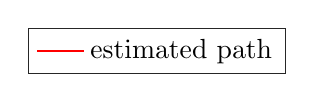
\begin{tikzpicture}

\begin{axis}[%
width=0.951\figurewidth,
height=\figureheight,
at={(0\figurewidth,0\figureheight)},
scale only axis,
xmin=-585.465549481059,
xmax=0.0310013961145614,
ymin=-48.0606441036616,
ymax=413.726151668819,
axis background/.style={fill=white},
legend style={legend cell align=left, align=left, draw=white!15!black}
]
\addplot [color=red]
  table[row sep=crcr]{%
-0.00529309643841828	1.21638477512972\\
0.0310013961145735	1.7752367963942\\
0.0296036613750634	2.18266008143797\\
-0.000898269043408784	2.77999136890411\\
-0.210193876803725	3.06574711781351\\
-0.366569983475035	3.43171135983982\\
-0.678705960072959	3.74041749392698\\
-0.292888057280307	4.39000268706999\\
-0.380204206131541	4.61430059201562\\
-0.518539019589657	5.22163426451259\\
-1.08535266569375	7.03121389247788\\
-1.43543545105854	7.71475228003225\\
-2.07144689005216	8.95500110359886\\
-2.12536337606111	9.46337045663576\\
-2.79522441067431	10.4376213044453\\
-3.38821974006266	11.2005890856601\\
-3.96087487422032	12.5329014816845\\
-4.18068091406808	13.2270702341543\\
-4.69514053620645	14.1601135539659\\
-4.95044671418723	14.732255011951\\
-5.74109008564688	16.4590551158276\\
-6.25864909810605	17.1651242341509\\
-6.92680045973068	18.0096852689948\\
-7.52721890019593	18.7326771524019\\
-7.89833485649408	19.6736655879446\\
-8.35366764409023	20.2527092667404\\
-8.97529170737234	20.8294346087104\\
-9.73644714325414	21.9150956873054\\
-10.2336895921104	22.4555510214841\\
-10.538049037341	23.4728674456969\\
-11.6352043115028	24.8562459805522\\
-12.427725448973	25.7663702529544\\
-12.8988765671607	26.6384731054816\\
-13.8603919485598	27.3074798274492\\
-14.2332375759338	28.2035567600315\\
-14.9323837750779	29.0081371030198\\
-15.5623828528675	29.9879355697692\\
-16.4382644892338	30.879603982934\\
-17.0462967341107	32.2332052350626\\
-17.6544661332664	32.2442769554075\\
-19.0804218642382	33.5929531466999\\
-19.8151060272339	34.3660755897687\\
-20.5185400984138	35.1025756147964\\
-21.2122325205373	36.0768222169785\\
-21.933323574914	36.5383956680607\\
-22.6783826876664	37.3080519019167\\
-23.265482208781	37.8997238927703\\
-24.1900429836478	39.0151997374315\\
-24.7064805398691	39.2583692299979\\
-25.6836980697829	40.2358342339721\\
-27.2343804732855	41.2691108384854\\
-27.9902326993395	41.6622290247058\\
-28.4559037023475	42.4497912882057\\
-29.1409328794516	43.245558804245\\
-29.729909746791	43.586519740246\\
-30.6155249028881	43.9141069641552\\
-31.0714694575924	44.5057196203637\\
-31.9173468655687	45.4661938097233\\
-32.4800417274997	45.667714848823\\
-33.2205407500732	46.362799710116\\
-34.6581377886863	47.4499636187366\\
-35.4263601119116	48.1793467689213\\
-36.3095756289785	49.0159726428835\\
-37.0042650297585	49.6282947925252\\
-37.767156010131	50.2746957869826\\
-38.730917373166	51.0987937401227\\
-39.3303894229672	51.7148146739813\\
-40.0519197235706	52.0174174104924\\
-40.8068382563655	53.0600439506135\\
-42.022836568752	54.0984596508611\\
-43.4917561089529	55.2850349004074\\
-44.1487857446373	55.9079974617928\\
-44.8652727937947	56.6102404991093\\
-45.6128972610143	57.2090634136114\\
-46.2045130544745	57.6261067737546\\
-46.9941764247739	58.3064578195943\\
-47.6410747152918	58.7081423780225\\
-48.2814719915542	59.1834548435738\\
-49.0375425094581	59.7964771246541\\
-49.7042377506045	60.258310889481\\
-51.1137569521862	61.4252529113835\\
-51.8653850992552	62.2418245126545\\
-52.5918031369244	62.757872931151\\
-53.405599217025	63.4216774510572\\
-54.0690545936713	64.1083363050123\\
-54.6826004342828	64.528788801098\\
-55.5598716933512	65.1967648742419\\
-55.9671247928558	65.4647363877011\\
-56.7914362970586	66.1755655210409\\
-57.4242085734627	66.5376459309436\\
-58.8584473431698	67.8106374811823\\
-59.4106778501816	68.3899840234282\\
-60.1973168038283	69.1303816100193\\
-60.8698476127824	69.4381448525102\\
-61.6662448467124	70.3646280430521\\
-62.27376243033	70.7295928996751\\
-63.088869838903	71.4550171693975\\
-63.8190204148941	72.062737644526\\
-64.4945466303431	72.7098687334165\\
-65.0936084464003	73.3119927532716\\
-66.6115900523631	74.422979881537\\
-67.1632799820451	74.768272333153\\
-67.9444460311285	75.4777806694072\\
-68.5859304541525	75.8921197442659\\
-69.0919164662715	76.2296490993419\\
-69.6717620461785	76.6264665065103\\
-69.5675552520123	76.4568319798365\\
-70.1684024838886	76.6827501669795\\
-70.1986881918481	76.735470433094\\
-69.996530150655	76.6839025449796\\
-71.3893522644302	78.0426806411649\\
-72.0592627621295	78.5258828631915\\
-72.6735023348654	78.8812771721613\\
-73.2873431381428	79.6132743065457\\
-73.9294932270407	80.1178260765914\\
-74.4267237953252	80.3493355548826\\
-75.1798419283712	81.0531873082963\\
-75.483518850798	81.3069950934446\\
-76.3551202624832	81.7011157790706\\
-76.8237302854019	82.0925657767538\\
-77.9818972035832	83.196976475692\\
-78.6240435322844	83.829245499315\\
-79.5422478162758	84.6317063407071\\
-80.249207696876	85.3015319321201\\
-81.0557020228346	85.6472155281485\\
-81.6052693094843	86.1594664967806\\
-82.4985743975442	86.8197366147005\\
-83.3926143160741	87.4015550221221\\
-84.0658933287809	87.8951227767075\\
-85.390992479137	88.6048052365402\\
-86.7890614449716	89.764957623844\\
-87.5685778618679	90.3984924877369\\
-88.3756256760647	90.8735170110521\\
-89.0661297320231	91.3309999477143\\
-89.8744806781423	91.868341459276\\
-90.8286671154953	92.3614889832572\\
-91.5460522714028	92.7457908260052\\
-92.2037601229347	93.2682562915529\\
-92.8587193534349	93.5737486429026\\
-94.0077128863083	94.172782697531\\
-95.791122389785	95.2987673112251\\
-96.4723171020035	95.7364441055299\\
-97.1154711683338	96.3482236981422\\
-97.7972493974098	96.8271452437785\\
-98.3536623621639	97.3687276902555\\
-98.928426528915	97.8701122625582\\
-99.6977055131553	98.3687804884692\\
-100.303522369389	98.8043199127252\\
-100.640186665367	99.3953291478742\\
-101.653719848538	99.8760407822796\\
-103.133390512053	100.997449615514\\
-103.836078790631	101.494368341855\\
-104.462110579774	101.90761307866\\
-104.90339366226	102.540363856133\\
-105.597229597919	103.030706764689\\
-106.199525495973	103.53040210164\\
-106.702154116732	104.008596510617\\
-107.317128981515	104.527125575309\\
-108.130769318645	105.156317734919\\
-108.65059056736	105.391230144609\\
-110.121179989917	106.437075578508\\
-110.774096488767	106.925375943871\\
-111.419542440686	107.526137237736\\
-112.241116097648	107.978975071026\\
-112.855719623446	108.576966606694\\
-113.517017565556	109.195992537029\\
-114.31453984163	109.542553445313\\
-115.106042400249	110.002463445768\\
-115.624887198669	110.732973145636\\
-116.378382544561	111.37949528355\\
-117.733361239708	112.456762963287\\
-118.608121755251	113.160242740502\\
-119.316759302132	113.834281813656\\
-120.096378535487	114.556708513321\\
-120.787622499625	115.086315811468\\
-121.659624942964	115.581453305896\\
-122.436070770335	116.139003119057\\
-123.211686502411	116.71543766178\\
-124.069738480824	117.458331905963\\
-124.766881026804	118.048716464199\\
-126.273201638355	119.129755790655\\
-127.063986541139	119.632656327597\\
-127.608609083982	120.044166679751\\
-128.242293364161	120.556168153651\\
-128.854970289858	121.077995297464\\
-129.50497877429	121.518248945799\\
-130.110217986509	122.014744654098\\
-130.716827782084	122.481146022962\\
-131.448188163889	123.009220899481\\
-132.122226481663	123.539229117827\\
-133.701334530637	124.799220480804\\
-134.288097322755	125.366321924084\\
-134.993143614202	125.972703646742\\
-135.777074183058	126.438843628149\\
-136.482283796448	126.917544099463\\
-137.229407894789	127.451541354591\\
-138.005061470596	128.010915051167\\
-138.891702337198	128.778503607856\\
-139.637468042794	129.300923158025\\
-140.499143842679	129.867984275267\\
-141.94744822153	131.147946535813\\
-142.693677964404	131.643771843885\\
-143.546529289378	132.264101021058\\
-144.295272446377	132.595227577241\\
-144.952473627924	133.262557618171\\
-145.689667551522	133.812550079541\\
-146.414752898334	134.30064899329\\
-147.199133772027	135.059697211023\\
-147.661501851665	134.710228821605\\
-148.686783317206	136.319417673232\\
-150.163355066847	137.630054871264\\
-150.748380843603	138.215362813183\\
-151.442610096949	138.56458703443\\
-152.211302567126	139.26403177327\\
-152.925458256107	139.727113111058\\
-153.621233059108	140.155544679384\\
-154.435789646426	140.951205402579\\
-154.889391046586	141.193952585448\\
-155.440717671821	141.550329504038\\
-156.157964145212	142.148761598447\\
-157.599222929105	143.277766791327\\
-158.335378879922	143.858430465801\\
-159.196222173522	144.612733390034\\
-159.960287786049	145.210510078995\\
-160.58599714749	145.734005041334\\
-161.401933249555	146.320042681047\\
-161.97093024247	146.756862863332\\
-162.786782040237	147.266463634733\\
-163.541713210239	147.907266234996\\
-164.326583220848	148.451827719639\\
-165.914448246761	149.675554461487\\
-166.648470655251	150.107820903257\\
-167.517977049366	150.851843266007\\
-168.294374362287	151.264440438242\\
-168.912932613919	151.688811780819\\
-169.52447344553	152.101947705046\\
-170.348884130514	152.49278694033\\
-171.021595317522	153.176202753994\\
-171.784018308238	153.557632436601\\
-172.627704948925	154.442478469257\\
-174.322897339848	155.790055171384\\
-174.913995593544	156.16111087033\\
-175.67645115165	156.634058645607\\
-176.321981695714	157.171338328887\\
-176.953399135686	157.72312690988\\
-177.555401397798	158.220133948792\\
-178.27859535833	158.427607435477\\
-178.685536505231	158.48266370481\\
-179.458224378124	159.424837836776\\
-180.029410882853	159.691744707612\\
-181.663416219169	160.872977886344\\
-182.56126392591	161.364073085615\\
-183.151400243738	161.829238869591\\
-183.979570310687	162.368667699307\\
-184.611743493135	163.031895088558\\
-185.26443585453	163.401824479751\\
-186.097064821434	164.110938584356\\
-186.647702474827	164.487546318255\\
-187.130789938398	163.99059872779\\
-187.901458397934	164.326018285201\\
-189.260376484164	165.344043602046\\
-190.048716075227	165.952463229884\\
-190.659067223846	166.41740055059\\
-191.374332137823	166.930479206029\\
-191.886868103075	167.330608613153\\
-192.476160429296	167.758151241565\\
-193.035887315858	167.910333040292\\
-193.635613952768	168.289628817061\\
-194.351911431996	169.026994811598\\
-194.840405516091	169.066467822914\\
-196.431282193881	170.191213946094\\
-197.068082922011	170.646186317885\\
-198.008155748497	171.523696901692\\
-198.977706422773	171.725316972632\\
-199.600839560855	172.0918490074\\
-200.37572900691	172.901232589847\\
-201.219003739454	173.083014408893\\
-202.048342040883	174.386941484311\\
-202.863393051228	174.796672090753\\
-203.838004394723	175.041418627963\\
-205.291723954078	176.073624799827\\
-206.121801214764	176.759536544718\\
-207.079912289906	177.411731350525\\
-207.788567655121	177.897089871658\\
-208.755665635794	178.699411869079\\
-209.430661605279	178.946721024586\\
-210.290044472786	179.619143131064\\
-211.132408486668	180.182770232009\\
-211.879174784558	181.011973465479\\
-212.899587549828	182.073922372084\\
-214.540908402505	183.191571580502\\
-215.226446862168	183.550534182911\\
-215.987678142024	184.086770663073\\
-216.820689798642	184.681226877239\\
-217.676395829037	185.248271707117\\
-218.408816328217	185.574848266384\\
-219.247115011116	186.323641890965\\
-220.059690621794	186.878124715355\\
-220.913409253407	187.645579892905\\
-221.860601123611	188.099833321423\\
-223.290560607157	188.949873814998\\
-223.924103179198	189.506510404997\\
-224.532784249032	189.949718607598\\
-225.239777293261	190.515367881478\\
-225.799408490486	190.845008548205\\
-226.230974347634	190.897536756556\\
-226.818085727868	191.137075240687\\
-227.493301674674	191.575432970737\\
-228.296757334148	192.089299900671\\
-228.976185236254	191.625224835493\\
-230.191305836808	192.72267440847\\
-230.94265636237	193.351933386631\\
-232.196036500723	194.140354645148\\
-232.712838955822	194.492884703215\\
-233.629195228421	195.287784192422\\
-234.330940155365	195.358718843195\\
-235.595609323091	196.644176914025\\
-236.155220883405	196.282949600333\\
-236.773613721569	197.325083668291\\
-237.595555792661	197.62590310901\\
-239.012967016612	198.513189350525\\
-239.711779133011	199.033602118506\\
-240.128292607589	199.284407756029\\
-240.672351133186	199.48911865739\\
-241.209931202553	199.671827192514\\
-241.836085767054	199.79261162323\\
-242.337132108478	200.393437235547\\
-243.361438683542	200.898305438638\\
-244.294964642623	201.823999289691\\
-244.7404329082	202.02186871351\\
-246.340684500443	203.31990970091\\
-247.026296539658	203.835798830174\\
-247.772761380417	203.943753999292\\
-248.348905392348	204.677455464217\\
-249.001123893616	205.143091385896\\
-249.559258905304	205.464672464292\\
-249.762975559632	205.673849604362\\
-250.387832126283	206.238162577047\\
-251.228311788429	207.169393203108\\
-251.612466049215	206.91926481156\\
-253.276491262592	208.047347244249\\
-253.978993067444	208.516391394391\\
-254.703074799093	208.906315715709\\
-255.402077063667	209.508721885441\\
-256.066530122344	209.811879878293\\
-256.912181022826	210.497805153858\\
-257.685251086112	211.025429581808\\
-258.370728378892	211.607781104743\\
-259.047581007321	212.031753619359\\
-259.683085222952	212.454955680121\\
-261.099393048925	213.523187194681\\
-262.035605622053	214.085185398533\\
-262.790181821603	214.745801192096\\
-263.53662032189	215.191392938062\\
-264.378741934285	215.867034343864\\
-265.122768485566	216.391837797689\\
-265.928072217202	217.001686411\\
-266.529975204628	217.409346535876\\
-267.361385087999	217.968835689768\\
-267.97228805423	218.525273111795\\
-269.643945204199	219.70564934904\\
-270.37528585764	220.274088108484\\
-271.160620832037	220.770099303535\\
-272.02858992241	221.346863295413\\
-272.840974019611	221.834533706023\\
-273.74041794576	222.529439998389\\
-274.564825541337	223.072912304303\\
-275.295140836811	223.45152902706\\
-276.166682237282	224.244617023334\\
-277.039031491665	224.755149191702\\
-278.615179872516	225.798839746213\\
-279.351600078332	226.381178838044\\
-280.153497060358	227.034101699673\\
-280.923289826388	227.308642565248\\
-281.724726101073	227.920938335315\\
-282.456065092692	228.552725553465\\
-283.137698838088	229.296252501107\\
-283.923141721684	229.408058768261\\
-284.663090082004	230.241914015535\\
-285.483729538215	231.068285082035\\
-287.094203973019	232.169113713638\\
-287.849950401323	232.704397836235\\
-288.526380186985	233.305305166107\\
-289.307893290512	233.808919408234\\
-289.982907290536	234.401096903627\\
-290.774224157044	234.7352288235\\
-291.43356875712	235.52582448475\\
-292.117832716392	236.192747252751\\
-292.950316240244	236.633722614332\\
-293.876678035053	237.231423902095\\
-295.343562208586	238.337674073561\\
-296.137548825205	239.035479270869\\
-297.045052525847	239.653777239528\\
-297.919036815677	240.171273928196\\
-298.468172242574	240.380695298704\\
-299.194787887501	240.909382724451\\
-300.116109035031	241.653009041412\\
-301.001070202467	242.665248823438\\
-301.671986618706	242.972101373588\\
-302.22746019442	242.972712923567\\
-303.772619059504	243.998633357658\\
-304.652152006151	244.703610923636\\
-305.451196662276	245.172325822523\\
-305.961557597526	245.333798308907\\
-306.718204009287	246.163546332175\\
-307.496259527112	246.534438885788\\
-308.315264340382	247.174829966219\\
-309.350697255751	247.756939475427\\
-309.906432098495	248.228434253859\\
-310.714675027383	249.022212849117\\
-312.352244920124	250.070476680042\\
-313.058316915631	250.52648635158\\
-313.934154830555	251.178607083447\\
-314.704674049974	251.529842602399\\
-315.44029230332	251.86214095522\\
-316.29164172158	252.541278243428\\
-317.133943628962	253.129818075353\\
-317.932822387396	253.858672220808\\
-318.601151671521	253.923178762062\\
-319.350757315802	254.309301269294\\
-320.924472371011	255.224245163023\\
-321.781165470481	255.659624698969\\
-322.614891542495	256.215201069173\\
-323.328557408438	256.561788690533\\
-324.182349507533	257.075144794046\\
-324.999814711691	257.610517682519\\
-325.829439445144	258.164029694501\\
-326.391193120415	258.553984791858\\
-327.088011125236	259.157071047071\\
-327.756381665825	259.649882717401\\
-329.288901985964	260.66256493271\\
-330.168560897712	261.22342310093\\
-330.815004728691	261.509550170186\\
-331.623725641576	262.017991813333\\
-332.359395528398	262.528384570146\\
-333.002463758361	263.126076094696\\
-333.839593491261	263.425222982864\\
-334.364502298568	263.543728599114\\
-335.120524543522	264.606976076005\\
-335.868737772159	264.800493685664\\
-337.346606571958	265.906548240575\\
-338.035644887736	266.419066600926\\
-338.968396385967	266.957700817343\\
-339.752868387426	267.601714259834\\
-340.42732340207	268.064269027503\\
-341.24673646025	268.674203528933\\
-342.005547655989	269.205204338004\\
-342.598962977847	269.872102804077\\
-343.496397708694	270.480244491109\\
-344.026069707317	271.0921535474\\
-345.473714698506	272.130149589314\\
-346.218314501141	272.767055553032\\
-346.964279408261	273.2044213558\\
-347.64517349346	273.676327582183\\
-348.432157914639	274.188369623847\\
-349.03560788494	274.752950375606\\
-349.79590247009	275.171598739644\\
-350.334665884617	275.664904472467\\
-351.197942389675	276.029014252068\\
-351.846968157099	276.47816247654\\
-353.473071647762	277.465312338929\\
-354.174564806371	277.96606601371\\
-354.927107351461	278.364419550531\\
-355.607803929988	278.747065632894\\
-356.388987706305	279.378918332937\\
-357.218575297295	279.773522302446\\
-357.845029753542	280.21748129362\\
-358.620695784945	280.748993730624\\
-359.273084774229	281.294763208426\\
-359.931617520994	281.798986803673\\
-361.491508316579	282.93959466552\\
-362.248407843533	283.566249260637\\
-362.963102414153	284.035271112276\\
-363.798670593675	284.634343269888\\
-364.677208531131	285.196455657534\\
-365.412404816684	285.559550925672\\
-366.19944004595	286.12099042903\\
-366.851585906438	286.392667832555\\
-367.746163860883	287.213727296457\\
-368.448863215565	287.533673381372\\
-369.928146838866	288.53159702557\\
-370.77399368141	289.109285274787\\
-371.694378999677	289.596965900653\\
-372.477497633204	290.098281445054\\
-373.170651222976	290.832425866806\\
-374.056394331168	291.269187366826\\
-374.812986269656	291.723013613525\\
-375.578501639505	292.188948087465\\
-376.344187395843	292.562275004102\\
-377.109636074762	293.115525216139\\
-378.608750300272	294.145396611394\\
-379.353392732346	294.55997381814\\
-380.061149246344	295.204457528192\\
-380.788115048671	295.541214889334\\
-381.343476539659	295.988370685767\\
-381.964260753755	296.641242773089\\
-382.949597683613	296.894627342066\\
-383.509766846547	297.621734173378\\
-384.378540738138	297.883458740444\\
-384.473946734413	298.167567483466\\
-386.084989573582	299.209944178353\\
-386.884112948744	299.84018697003\\
-387.683665259584	300.304949365403\\
-388.519882569997	300.977275710964\\
-389.175740333891	301.326284241158\\
-389.861906176397	301.997713776841\\
-390.742875915031	302.305265172023\\
-391.409748894408	302.811060129054\\
-392.075994099464	303.208199571761\\
-392.851351256214	303.86505745769\\
-394.376312250403	304.911072872614\\
-395.138824369961	305.488234928868\\
-395.990075399087	306.184659466926\\
-396.808590619708	306.681145896009\\
-397.615829494443	307.153499637612\\
-398.310981979145	307.82059762802\\
-399.185988490143	308.36026644835\\
-399.996232157166	309.219786198164\\
-400.869370110575	309.682894832428\\
-401.684515168414	310.166889090417\\
-403.38027252444	311.27268837623\\
-404.1023994286	311.845623495339\\
-404.892746765128	312.348126342805\\
-405.699276088217	312.950365362675\\
-406.651786326596	313.368785219184\\
-407.330589214022	314.128001167122\\
-408.25697817899	314.82252679772\\
-408.964717949173	314.915287665289\\
-409.647632057834	315.451108089625\\
-410.530627213265	316.152149579452\\
-411.965308328076	317.103172026579\\
-412.690689080654	317.56446464542\\
-413.428183629928	318.104684424717\\
-414.150427074182	318.532008292586\\
-414.835779854138	319.034624359502\\
-415.491075714876	319.563335707582\\
-416.24389399306	319.969672791471\\
-416.885471216836	320.427112645627\\
-417.674119573777	321.158133838715\\
-418.24670661625	321.629188527119\\
-419.788873166292	322.782108859708\\
-420.468529711748	323.431991705445\\
-421.14024659637	323.707302151932\\
-421.676253068163	324.12607301436\\
-422.234812401121	324.38996667582\\
-422.886593262657	324.851376423381\\
-423.439196817747	325.287301635508\\
-424.01165130876	325.470041987995\\
-424.697175569987	326.306291090074\\
-424.31353152997	325.647914476753\\
-426.114143346587	326.939334724889\\
-426.651605609438	327.371486508938\\
-427.401654906608	327.947275268628\\
-428.369609987675	328.753336767121\\
-428.44741163239	328.662581038561\\
-429.648921727375	329.36320425068\\
-429.964197956279	329.546195158375\\
-430.607684823142	330.328202489006\\
-431.359322315916	330.66908848481\\
-432.94079451724	331.363144640256\\
-434.716639289413	332.496114564028\\
-435.290327456718	332.932772776683\\
-435.57916737625	333.214647182832\\
-436.556846935192	334.110821169223\\
-437.464155718942	334.48370559194\\
-438.360182638157	335.014230470998\\
-438.797507649893	335.510246642611\\
-439.764895927849	336.148441214677\\
-440.50132318918	336.624612495682\\
-440.65876432272	337.311174647289\\
-442.122788791946	338.131615552504\\
-442.545930795588	338.3036038543\\
-443.21776752569	338.893783986575\\
-443.577566805077	339.02077783527\\
-444.177131516196	339.495079362992\\
-444.622936717404	339.895449557467\\
-444.673142256469	340.2442128915\\
-445.495783011847	340.270487234621\\
-446.922932103207	341.191406440217\\
-447.338914520136	341.582616834862\\
-448.374669595624	342.136651101268\\
-448.801848005009	342.511225167232\\
-450.073400526519	342.997813195388\\
-450.996284516203	343.111575857998\\
-452.035818352142	344.452259896914\\
-452.710162300986	344.481525488788\\
-453.4813867162	344.93169906711\\
-453.777715096147	345.522996006108\\
-455.136168144158	346.55997658879\\
-456.01947856427	347.242868091408\\
-456.570147372897	347.738037233487\\
-457.21582737362	348.342796298511\\
-457.609760885716	348.435700494123\\
-457.755729561445	348.036266759689\\
-457.482733659153	348.242004665955\\
-458.462646345171	349.123005312038\\
-458.834690356938	349.043783927316\\
-459.042329493719	349.455806682708\\
-459.323378493386	349.084325163156\\
-459.519538176255	349.33960858616\\
-459.576414221637	349.397475651621\\
-459.797173435797	349.418521509968\\
-459.805046531289	349.348654854015\\
-459.972684928892	349.494542587258\\
-460.071469598006	349.230109332626\\
-460.160163328631	349.423527204051\\
-460.351953279958	349.561040974309\\
-460.318347278604	349.269411483231\\
-461.868024216231	349.998181087243\\
-462.457516359941	350.331625424024\\
-463.321430585846	350.947226478415\\
-464.110350451148	351.169931569939\\
-464.608386962404	351.702551577871\\
-465.669055941919	352.105443883695\\
-465.931689881883	352.491565637186\\
-467.05530889979	352.792095625991\\
-466.693857933521	352.787454595582\\
-467.662142494854	353.018033127255\\
-469.423867156497	353.953949907806\\
-470.253264735998	354.522963252208\\
-470.465665342132	354.668149058895\\
-471.2687186759	355.024421412963\\
-472.378026432929	355.652753751798\\
-472.352308814483	355.402421835058\\
-472.803240491577	355.730428699587\\
-473.986597764265	355.725813442119\\
-475.004018751984	356.625976636737\\
-475.977987030708	356.987658756485\\
-477.797430225003	357.710365086293\\
-478.32452329341	358.084115322175\\
-479.04332148349	358.310023561043\\
-478.714487020792	358.017021428097\\
-480.155490219351	358.491540431694\\
-481.065566492212	359.203646148239\\
-480.986500352812	358.729860786697\\
-482.310129055367	359.557805334904\\
-482.085373493062	359.750697523394\\
-481.064067326609	361.067867895277\\
-482.773075266758	361.561420954309\\
-483.15772597855	361.778059709128\\
-484.210824553624	362.011085324325\\
-484.814724951527	362.257150131186\\
-484.612643468268	361.730431893431\\
-485.305390496443	362.061977125422\\
-485.453260733687	362.020590604376\\
-484.860070394524	361.413637662145\\
-485.36216306443	361.445350728318\\
-484.977366231277	361.188198747307\\
-486.574212567322	361.617422157768\\
-487.11305057255	361.740535257653\\
-487.697758963528	361.583071656023\\
-488.598304560297	362.02876143639\\
-488.830642559916	361.802185098743\\
-489.527410629061	362.052240006188\\
-490.147328257154	361.840207307305\\
-490.823764540816	362.394168071252\\
-491.791679525499	362.668963507987\\
-492.389727216774	362.790945482464\\
-494.398623430722	363.334626905303\\
-495.766745055315	363.265575276255\\
-496.765345299142	363.439948789086\\
-497.103189795633	363.582828784468\\
-498.389546004058	363.770907117892\\
-499.342785054205	363.846827646485\\
-500.506285660215	364.174319966055\\
-500.828858112794	364.069162281963\\
-501.876646711665	364.162505488035\\
-502.874971693162	364.313450733866\\
-504.349535929467	364.449122790027\\
-505.759044087782	364.244787059695\\
-506.835596415278	363.996203011515\\
-508.094602360855	364.180978170413\\
-509.001721666651	364.056660156807\\
-510.064460180116	363.956120060927\\
-511.26338381363	363.842343246474\\
-512.15449804751	363.480082197421\\
-513.749033926765	363.244195688751\\
-514.698547638725	362.726268453164\\
-515.432381802637	363.360112886725\\
-515.916897951458	362.883698861051\\
-515.575159802466	362.400415683267\\
-516.413437457506	362.897568835384\\
-516.703573793504	362.751223719558\\
-517.43608162689	362.629848975304\\
-517.395435326263	362.400658754518\\
-518.024751173192	362.41294285826\\
-518.142089597948	362.031707135287\\
-518.566395169891	361.904297254364\\
-520.021777075289	361.857717039691\\
-520.319493083093	361.737458103904\\
-520.776476163184	361.531100425427\\
-521.351959783119	361.340753658486\\
-522.569810238252	361.232763859566\\
-523.008709723275	361.167805545977\\
-523.679206940351	360.877265360911\\
-525.339454972578	360.736435746986\\
-525.694468279029	360.871016946525\\
-526.389154367222	360.179742758699\\
-527.721157052505	359.141933705924\\
-528.09685061543	358.899145786271\\
-528.812927019438	358.378022431049\\
-529.535892294634	357.608266524866\\
-529.850425377453	357.392592954551\\
-530.484072117396	357.009789882685\\
-530.928079671445	356.349212715798\\
-531.646518149468	355.658569694188\\
-532.127617081567	355.049977173899\\
-533.44376684319	354.491401702238\\
-534.381983865857	353.513705574277\\
-534.620015535754	353.322218254188\\
-535.149936807506	352.80717178886\\
-535.33284118026	352.599923272005\\
-535.788597817115	351.96996151341\\
-536.170867873037	351.65427802909\\
-536.511014981442	351.28633052115\\
-537.006844093265	350.871644962896\\
-537.154915421228	350.582455224698\\
-537.747474477197	349.987776380507\\
-538.2795893675	348.932538873644\\
-538.937651916827	348.239441834859\\
-539.240314973339	347.65031660341\\
-539.30508339487	347.134948778325\\
-539.829264876329	346.729602645106\\
-540.398319391383	346.390338219592\\
-540.345618744639	345.776410721656\\
-540.844351917498	345.228749990268\\
-541.05674640544	344.653203119825\\
-541.498535989118	344.333069627239\\
-542.221793021408	342.942021590525\\
-542.550455354317	342.420951697369\\
-543.22797108822	341.572119056728\\
-543.281358766404	340.993961844305\\
-543.734149572752	340.41891352873\\
-543.49620650555	339.925524827768\\
-544.235243444307	339.321885927446\\
-544.455926193477	337.989769677993\\
-544.99324366642	337.230806575208\\
-544.845802195916	336.206131390659\\
-544.912574062337	334.883524298892\\
-544.927750518101	334.2845549227\\
-545.256870228055	333.635265899205\\
-544.981938228219	332.977378215897\\
-545.571871266012	331.430338468929\\
-545.080633640324	331.254588913451\\
-545.598802849932	331.789369106642\\
-545.830694830114	330.526185941019\\
-546.063813497827	329.562088991808\\
-546.291911169519	328.869071717662\\
-546.449844911911	327.128941452612\\
-546.557679367031	326.220888175959\\
-546.425344733941	325.361032302756\\
-546.260027305331	324.908459080294\\
-546.302859778969	323.810826136224\\
-546.007100897798	322.944674444417\\
-545.669930453594	321.948002481361\\
-545.464181895387	321.714104688261\\
-545.565527461772	319.867813228277\\
-545.274550617143	319.561321974342\\
-545.269183765622	317.913863739451\\
-545.273201344414	317.030479239388\\
-544.738230440378	316.1033182694\\
-544.62747108626	315.515934627123\\
-544.736377253068	314.309969734006\\
-544.156740864036	313.919940701832\\
-544.435826930652	312.891541073532\\
-544.197805839325	312.17887731445\\
-544.229584509485	310.93573180135\\
-543.897149260372	310.626029585714\\
-542.938366377689	309.391999521399\\
-543.064613263017	309.296621500772\\
-543.025880747658	308.794742757146\\
-543.082652567422	308.376391882782\\
-542.689333550279	308.541755106421\\
-542.314799488933	307.921459722606\\
-542.682191365307	307.193824036715\\
-542.665209775309	307.202723345042\\
-542.867575499771	306.085039622195\\
-542.551307828523	306.048419645611\\
-541.950889520087	305.15444243347\\
-541.519886009438	304.458605816985\\
-541.379929755703	304.00637570123\\
-540.810201564881	303.307901008768\\
-540.439575074775	302.162903654905\\
-540.392670615668	301.931608284873\\
-539.967728559033	301.581541145421\\
-539.734521497236	300.262432813222\\
-538.598209429551	299.897943405363\\
-539.334806655551	300.229075637029\\
-539.320289393156	299.349483704892\\
-538.366321701848	298.764919823441\\
-539.02413455695	297.814221057231\\
-538.807770240042	297.271403572871\\
-538.595826030623	296.630528559128\\
-538.392593894564	296.517187531233\\
-537.815383285211	296.301396019333\\
-537.303480474678	295.934859123142\\
-537.029196345789	296.883774544738\\
-537.717634343635	296.318869253839\\
-537.192144533982	295.655605237325\\
-536.632923143613	294.935455753136\\
-535.929154555539	293.510741856666\\
-535.693586292434	293.07584389022\\
-534.558073607083	292.386154319406\\
-534.531602918181	291.43576918269\\
-533.877805941366	291.378503543971\\
-533.828356854265	291.011272081451\\
-532.509735122794	290.305545373006\\
-531.850431086894	289.659584431986\\
-530.883787337704	289.210552725569\\
-530.304059024786	288.817550411356\\
-529.831827268368	288.641318555613\\
-529.902891757969	288.692409779837\\
-529.082649897884	288.089928028588\\
-528.75769308073	287.922315635085\\
-528.1829005595	287.763673229858\\
-528.036028231463	287.714707098436\\
-527.929963978753	287.451214872921\\
-527.034594364346	287.47781048978\\
-525.89458798002	287.420552942451\\
-525.93643437972	287.422208443417\\
-525.244141043193	287.387923787985\\
-525.164945897234	287.367013589393\\
-524.808139248151	287.318959477209\\
-524.65616980741	286.791547446237\\
-524.460401907732	286.519611238127\\
-524.07317423879	286.409427202384\\
-523.924716665435	286.278300238871\\
-523.465223406884	286.262685653773\\
-521.920717014364	285.191902470355\\
-521.297113876477	284.687768525799\\
-520.667123118262	284.228978612048\\
-520.186678656113	284.112565769583\\
-519.48056170838	283.837962967027\\
-518.984261052807	283.425841595687\\
-518.492966614878	283.160909063104\\
-517.970102570179	282.86297080194\\
-517.758508488514	282.572945477112\\
-517.068433040134	282.525294107728\\
-515.777944982568	281.556257364519\\
-514.870390433331	281.036979556713\\
-513.605613794053	280.286865364038\\
-512.742653867753	279.732791868924\\
-511.753130454039	279.123034133742\\
-510.195859413966	278.553209435657\\
-509.38895339775	277.91923573479\\
-508.352083291482	277.502171716158\\
-507.682634072241	277.206229326474\\
-506.68506346317	277.173028165228\\
-505.30908865183	276.435387890394\\
-504.244882470177	275.76603467594\\
-503.696494754539	275.403561260122\\
-503.563676955721	275.518630517636\\
-503.08698679473	275.181639311565\\
-502.281099528506	275.230354075972\\
-501.889921219274	275.114215410818\\
-501.363414006679	274.702919239128\\
-501.040012415525	274.156425739043\\
-500.61976253059	273.866415784564\\
-499.003010173012	273.054641251673\\
-498.234362284753	272.574486014734\\
-497.478223867246	272.208224495891\\
-496.776750380101	271.875283594694\\
-496.307250254938	271.574020070837\\
-495.372641434241	271.200493294902\\
-494.543487363037	270.835426408021\\
-493.994211964344	270.488545217243\\
-492.619219649705	270.173219873766\\
-492.255523263803	269.818382282127\\
-490.473369900332	268.96891569602\\
-489.710656237249	268.656652229748\\
-489.050162458449	268.293154696157\\
-488.245672375228	268.105349351316\\
-487.310414841543	267.669759659395\\
-486.61808444406	267.28538471625\\
-485.758410802403	266.674207102944\\
-486.734349929612	267.133351691526\\
-486.115569548848	266.331832977159\\
-486.335839714766	266.052703198367\\
-484.730042871806	265.61491432533\\
-484.678992170216	265.411392735419\\
-484.351478915163	265.104407931755\\
-483.837755901752	264.873259998716\\
-483.034325186316	264.391416629982\\
-482.749966160285	264.185971487186\\
-482.273108104067	263.498538895573\\
-481.527075426772	263.279263040238\\
-480.671851873545	263.146182025379\\
-479.76526523887	262.869696697542\\
-478.200456190387	262.055824072118\\
-477.626570540046	261.82278231571\\
-477.568169622306	261.563391163742\\
-476.95778245093	261.442702586897\\
-476.451582662925	261.213371939998\\
-476.09189990416	260.944064211911\\
-475.720765700091	260.649524465042\\
-475.789747788672	260.440616016271\\
-475.199164026795	259.903792073936\\
-474.334949546526	259.800588615172\\
-472.646653285571	258.633908268911\\
-471.797764706654	258.060439989539\\
-471.377170629058	257.626621754788\\
-470.147126643433	257.337081300116\\
-469.663912845103	256.72879085771\\
-468.762687563579	256.232372801396\\
-468.322591783775	256.024437320114\\
-467.318759835204	255.666985509326\\
-465.937213011501	255.103627388485\\
-465.418018729445	254.752317862228\\
-465.417239844225	255.073064973012\\
-465.23005268983	254.588270015427\\
-465.278883663178	254.338651199111\\
-464.884325701519	254.081498316423\\
-464.473864374326	253.695803196766\\
-463.364916225995	253.560825411376\\
-462.751205711956	253.350696033999\\
-463.11075822995	252.753759166754\\
-461.759738011138	252.968211197966\\
-460.903523933923	252.658878722694\\
-460.797059213963	252.501040227496\\
-460.361460386027	251.428950933366\\
-459.918601138651	250.913295573499\\
-459.429804523708	250.537758033368\\
-458.589496697227	250.370517600302\\
-458.185599918634	249.632489630999\\
-457.902208614884	249.634332418624\\
-457.508554462249	249.930730045197\\
-458.611910440196	249.884771623326\\
-458.968621485685	249.826501290683\\
-459.344775253415	249.716535014533\\
-458.332207300769	249.439336228298\\
-458.356053996745	249.308774860988\\
-457.888328186479	249.162596525633\\
-457.588878419303	249.023165339071\\
-457.433010465333	248.87084380513\\
-457.340905014626	248.697011247924\\
-457.000755999631	248.5153073027\\
-455.473293476856	247.591449888631\\
-454.98916550757	247.362383999611\\
-454.153237993958	247.069392505449\\
-453.303901498923	246.79396350504\\
-452.734550950991	246.536537269211\\
-452.114687197901	246.300649988953\\
-451.950756611108	246.198448668559\\
-451.128626588611	245.897127685361\\
-450.737382133884	245.687115874503\\
-450.653313792483	245.541555973186\\
-449.27045521713	244.736777443056\\
-448.528812132245	244.521025661615\\
-447.774290105374	244.246079882791\\
-447.242642221934	244.001486604719\\
-446.702326958636	243.702664520243\\
-446.325139533663	243.413977964341\\
-446.258494620166	242.822413671181\\
-446.466107100934	242.614260764643\\
-446.291809432449	242.581730864089\\
-446.106683716401	242.246713745388\\
-446.845516733257	242.309572639886\\
-446.476333946971	242.163182472176\\
-446.347683637068	242.026867785381\\
-446.104645844354	241.832011138837\\
-445.6671096707	241.64106993552\\
-445.251664940493	241.434548057467\\
-444.591424581771	241.52144148074\\
-444.328574427155	241.496717356412\\
-443.92850724349	241.32026659462\\
-443.357229041238	241.289421706548\\
-441.806805873162	240.204380580382\\
-441.191065722479	239.751431948242\\
-440.48419448546	239.341002961122\\
-439.962075369104	238.59549648441\\
-439.486858754145	238.412917113508\\
-438.572736824031	237.430063947579\\
-437.88226357864	236.560723461057\\
-437.311693699969	236.167771906879\\
-436.670824179541	235.491089849663\\
-434.876988134997	234.253797327502\\
-433.973568972179	233.859110923058\\
-433.27195166724	233.22521863758\\
-432.601510676348	232.850362963724\\
-432.021887988672	232.335817469479\\
-431.590132931931	231.905983064177\\
-430.694677353021	231.54549092895\\
-430.581391687325	231.811367582502\\
-430.187650024653	231.547784571234\\
-429.843238665214	231.200468058693\\
-428.52025470297	230.35485308446\\
-427.963050914632	230.036753213566\\
-427.359870429392	229.7085224572\\
-426.857578645347	229.404201316633\\
-426.41362485555	229.051865230043\\
-425.90955519615	228.687289753407\\
-425.509898797096	228.506362052233\\
-425.063709125303	228.113724918763\\
-424.670133288126	228.075040648657\\
-424.082293546792	227.722547343365\\
-423.541589263933	227.959962613729\\
-423.41158436067	227.82686740875\\
-423.110691501792	227.772078743977\\
-422.911877662163	227.244998975213\\
-422.604341540071	227.192920619518\\
-422.545194529247	227.662682527885\\
-422.472527185255	227.527906256634\\
-422.461018727008	227.404000575697\\
-422.208551752646	227.163274075403\\
-422.141372639264	227.067538186583\\
-420.695622892327	226.085849852664\\
-419.987123798021	225.616585405215\\
-419.12792936112	225.094840985742\\
-418.891167006826	224.677014742117\\
-418.204771985013	224.392849374178\\
-417.956270071597	223.6609292514\\
-417.554537376189	223.006187148469\\
-416.933191035587	223.250375055323\\
-416.744535034427	222.312001319748\\
-416.342939124494	221.694871015343\\
-414.707592775807	220.67193105781\\
-413.933395563679	220.036738596685\\
-413.484646041928	219.853336600274\\
-412.79992714228	219.4275639059\\
-412.287799884202	219.299933240701\\
-411.127550815765	218.569817878106\\
-411.651197185674	218.721310753444\\
-411.720345431738	218.241044474039\\
-412.088121463696	219.231951555444\\
-411.254606949033	218.418659462575\\
-409.791006984223	217.491949024273\\
-408.921299188693	216.732051777731\\
-408.308753689065	216.581223722549\\
-408.048905660549	215.664408954656\\
-407.545449072177	215.734155589441\\
-407.064225720305	215.304227919517\\
-406.259818365202	214.667843402177\\
-406.693896726785	215.038353293486\\
-406.203801451759	214.330969228495\\
-405.764341527872	214.06437960483\\
-403.863283837504	212.657268680081\\
-403.598047967658	212.457007205429\\
-402.919896976474	212.041231885064\\
-400.485349397088	210.618645174333\\
-399.19530348575	210.416335128534\\
-397.587201263411	209.735363118025\\
-395.880976657275	208.868410117225\\
-396.759417647589	207.559139438563\\
-395.284679404958	206.883438147408\\
-394.894565455108	206.354906649484\\
-394.080496850424	205.750722588345\\
-392.454984788071	204.982853578026\\
-392.584022950573	204.28829036593\\
-392.499655229643	203.782490670409\\
-389.997175236085	203.598675073202\\
-389.227625404401	203.303733325796\\
-389.345476705741	202.23145083253\\
-388.498231158981	202.423026378845\\
-388.420674610847	202.241226520618\\
-388.24026496449	202.246502409134\\
-388.376752292224	202.126017348926\\
-388.284522067554	202.205537349881\\
-387.814639576014	201.708348471804\\
-387.76294712182	201.740375279973\\
-387.883539441107	202.134770887625\\
-387.713965829213	201.569223599381\\
-388.014292368563	201.72284346235\\
-387.561617484187	202.103808345099\\
-387.582616083798	202.077694613751\\
-387.458090619629	202.075989754699\\
-387.417684421817	201.90486234542\\
-387.50462134448	202.161604446449\\
-387.396806646462	202.098254018096\\
-387.191709391429	202.267046869481\\
-387.082510576921	201.789859672918\\
-386.943658158228	201.683703020322\\
-386.563259797413	201.613267085443\\
-385.322851902255	200.710244362098\\
-384.453656050058	200.270249078023\\
-383.961780224134	199.969289757646\\
-383.507734399166	199.647366128492\\
-383.010300120296	199.421600075795\\
-382.421510122179	198.938277315406\\
-381.938093079012	198.564986958884\\
-381.431720596309	198.166224450254\\
-380.591786369224	197.594424156305\\
-380.854968174384	197.438597360523\\
-379.40273339416	196.614921880483\\
-378.422852795215	195.845908364975\\
-377.66084484537	195.534181079242\\
-376.704193150758	195.008256542388\\
-376.057098345862	194.611112307482\\
-375.485518644103	194.345468848076\\
-375.725372725498	194.350231813297\\
-375.318106533684	194.064775309544\\
-374.478010970199	193.700415500316\\
-374.045193860173	193.383092347822\\
-372.506581645378	192.564288772883\\
-371.638783633844	192.207754007598\\
-370.64876447365	191.84551438672\\
-370.236676533517	191.563387145941\\
-369.55505816398	191.183449991429\\
-368.923258810089	190.709780861756\\
-368.291649222544	190.266391613336\\
-367.540600164458	189.593650527927\\
-366.650402534451	189.153568881966\\
-365.605408552264	188.61849714655\\
-364.016325927949	187.639123843437\\
-363.201167806428	187.269342216665\\
-362.309224727019	186.746494499094\\
-361.612528331086	186.154418143893\\
-361.044560618982	186.009630869889\\
-360.277632392803	185.612660102708\\
-359.297785761524	185.052211575755\\
-358.415034610171	184.664507636325\\
-357.656199033359	184.226542704698\\
-357.042387897843	183.853223978687\\
-355.419286092211	182.780943788667\\
-354.529009244805	182.223126987209\\
-353.529245996153	181.742131835302\\
-352.621585776527	181.12730992191\\
-351.627739510897	180.707380104992\\
-350.620974410106	180.06441802794\\
-349.739453432124	179.586917524131\\
-348.61843792177	179.072295920381\\
-347.761041040996	178.498705943406\\
-346.866739722162	177.862679055264\\
-344.955540502211	177.331526863123\\
-344.198233780391	176.966720107568\\
-343.251068503715	176.62073698019\\
-342.706616711013	176.492784500614\\
-341.997778463723	176.303476085733\\
-341.601739090203	176.087941465659\\
-341.13871593369	175.839754567049\\
-340.531246205752	175.534917855381\\
-339.916787182137	175.148932255651\\
-339.351441725025	174.858747278424\\
-338.576109333503	175.255462824145\\
-338.540176824403	175.200650691043\\
-338.517109378259	175.150965522409\\
-338.409497792829	174.984332475202\\
-338.182276488049	174.778070116262\\
-338.096452037984	174.792676940016\\
-337.504261981459	174.26599284194\\
-337.279659171456	174.449042247719\\
-337.546342037565	174.591482909745\\
-337.518249968675	174.505673179909\\
-335.91048162071	173.840638228328\\
-335.674313783445	173.81514699238\\
-335.402887671821	173.611140839734\\
-335.278894494585	173.512287802829\\
-334.841271341968	173.38345297473\\
-334.564355297214	173.268002339284\\
-333.997492162887	173.096219039193\\
-333.485863166297	172.785039800158\\
-333.078273117213	172.493998704651\\
-331.834796117165	171.859023968446\\
-330.077337315018	170.997503910279\\
-329.268225288455	170.470414549175\\
-328.258872635376	170.108489287897\\
-327.75493404234	169.606887300904\\
-327.089838013853	169.159568023757\\
-326.563493724777	168.786921917409\\
-325.800294508785	168.441174971516\\
-325.143589620058	168.193821361016\\
-324.872430498316	167.724495608353\\
-324.153790879579	167.292438848138\\
-322.447491025794	166.302522278598\\
-321.731182713608	165.946404794677\\
-321.069054697342	165.461738056064\\
-320.088348530722	165.082523944908\\
-319.564390292206	164.66910505057\\
-318.682177137229	164.300496521682\\
-318.465586314215	163.850443183147\\
-317.902304176604	163.62348631067\\
-317.598442243771	163.037041896528\\
-316.642504256244	162.592164016451\\
-315.185867772198	161.721936788367\\
-314.556661885494	161.194258945682\\
-313.775507222287	160.724698507283\\
-313.258422575822	160.354798592066\\
-312.627891485027	159.894518012458\\
-312.0837592389	159.479435486827\\
-311.372904156167	158.750658245775\\
-310.697869086309	158.35205342462\\
-309.936931312742	157.654328830654\\
-309.280540407667	157.134254539621\\
-310.44514944785	156.410942161445\\
-308.424104348178	155.7864876961\\
-308.730806656583	155.183898337014\\
-307.942370951203	154.674982636705\\
-307.360713884873	154.237861399474\\
-305.811666061636	153.734241686799\\
-305.225045662018	153.110270758237\\
-303.526647486516	152.965844401568\\
-303.783798972464	152.324656269658\\
-302.98372936265	152.372407504036\\
-302.356940713892	151.948981149076\\
-301.721050913889	151.795292049559\\
-301.501850569149	151.432571057811\\
-300.865027040659	151.123259370356\\
-300.104409613719	150.707030469003\\
-299.437262411211	150.574032097497\\
-298.684558853484	150.375864378118\\
-297.807572111764	150.104214933209\\
-299.187686719915	149.819584708446\\
-298.631240611808	149.583693286251\\
-297.09372479574	148.659508408184\\
-296.138686690939	148.376059976977\\
-295.654590816551	147.997917871946\\
-294.859597543775	147.620634132343\\
-293.791045507892	147.374480352383\\
-293.223951942041	146.891524094831\\
-292.382343962778	146.659673399702\\
-291.419778294044	146.360040795672\\
-290.846402060867	146.049229886952\\
-290.625499277403	145.59788538456\\
-289.00007231669	145.594838285508\\
-288.369489525758	145.568014820552\\
-287.986136850021	145.473734225911\\
-287.645830635042	146.337722072618\\
-284.970350741	144.508624638475\\
-284.359479778921	143.511464076501\\
-284.16964846095	143.083508629443\\
-282.112325075497	142.692820975981\\
-281.159901763055	141.148748403642\\
-281.13826697966	140.336415393735\\
-279.59476697595	139.459495719753\\
-278.751547076608	138.938103706249\\
-278.006399109164	138.411717913288\\
-277.236966917838	137.854838907639\\
-276.762241828276	137.659651251452\\
-276.107150407618	137.204788577308\\
-275.425480556708	136.829058593464\\
-274.622282833272	136.272444885415\\
-273.94942901496	135.831990135881\\
-273.441874242052	135.571852580525\\
-271.935456188555	134.951265112582\\
-271.315626421381	134.677747854035\\
-270.89307367244	134.555588722476\\
-270.351798093856	134.302703444087\\
-269.903711657808	133.891482657056\\
-269.428478220959	133.623150055612\\
-268.754356778919	133.342791170356\\
-269.566799766977	133.414352197646\\
-269.453158605228	133.371722722822\\
-269.473399969562	133.292252933241\\
-267.612064138359	132.351583937779\\
-267.074979267913	132.111519357103\\
-266.395857263929	131.683709986487\\
-265.650814462098	131.290840416943\\
-264.84178004128	130.927227313438\\
-264.632393305122	130.792908603188\\
-263.223827870947	130.110456439048\\
-262.885350479222	129.867552273658\\
-262.144878407349	129.239382882594\\
-261.394178607891	128.799526350632\\
-259.792677600646	128.090067050748\\
-259.094362245032	127.570987401436\\
-258.063174980605	127.086647429918\\
-257.613310489265	126.643843031068\\
-256.511791921907	126.120902599055\\
-255.854853360817	125.811624957235\\
-255.513967245393	125.419571326328\\
-254.144281699666	125.011666499509\\
-253.589479759324	124.672511287476\\
-253.246143626901	124.933942626041\\
-252.013543011939	124.404527924193\\
-251.913798281129	124.629536339291\\
-251.34111611439	124.270943186101\\
-251.128047145828	124.227203029999\\
-250.85339011919	124.106154148374\\
-250.401038535041	123.737945668217\\
-250.156777848031	123.890046698904\\
-249.732421231206	123.945619171391\\
-250.021427321993	123.727185398169\\
-249.800330780137	123.6826000624\\
-248.365692917851	122.724255056532\\
-247.768292436591	122.415340311093\\
-247.307136277786	122.336995332372\\
-246.883710066948	121.934497528453\\
-246.196043993897	121.556204352528\\
-245.763409286493	121.422468405901\\
-245.221469513803	121.210928376046\\
-244.680784539294	120.800369412487\\
-244.570637287456	120.568730067772\\
-243.860014985691	120.583433546101\\
-242.518784625202	119.868317203628\\
-242.3100062886	119.612121046792\\
-241.67639827351	119.263408768836\\
-241.200415394245	119.030633243257\\
-240.60333018033	118.590817930225\\
-239.985180449759	118.308065472093\\
-239.797815288156	118.17113138892\\
-239.061926631955	117.617091442511\\
-239.070327874431	117.586065186576\\
-238.73471287301	117.56150649576\\
-238.417019874974	117.939290166935\\
-238.296799184674	117.928770243445\\
-238.159520796591	117.924663872713\\
-238.182839552664	117.976906823652\\
-238.016605244522	117.839930702354\\
-238.174504065415	117.860718805194\\
-238.088749681131	117.800625076404\\
-237.862557504369	117.752362374515\\
-237.955777576189	117.688895375175\\
-237.668384940682	117.614886878989\\
-236.355117386743	117.003574482081\\
-236.169576546873	116.804588445311\\
-235.681423324161	116.657385954546\\
-235.054655791281	116.468142615532\\
-234.716627733391	116.271312459825\\
-234.946311021979	116.196684297279\\
-234.494075655313	116.007689571909\\
-234.600737126289	115.936738320993\\
-233.507499276345	115.685755288314\\
-236.167314077283	116.458602032584\\
-234.830069984127	115.673525414862\\
-233.982291789673	115.360901216383\\
-233.366028637258	114.909084479396\\
-232.859017427913	114.728957898249\\
-232.363719313227	114.379840550643\\
-231.60015563396	113.98410164783\\
-231.001551272489	113.838637783022\\
-229.503790239141	113.117448702892\\
-228.908118887215	112.634762943887\\
-228.312434340355	112.187423876186\\
-227.746020312361	110.795121095269\\
-226.691137983957	110.647216920462\\
-226.903319180722	109.909559197919\\
-226.803869964775	109.111215303146\\
-226.590027533119	109.605432917616\\
-226.175795608865	108.681589215463\\
-224.655127784107	108.432613380173\\
-224.321600181115	108.635806813724\\
-223.045284586334	108.12849351742\\
-220.844253961434	108.418569919954\\
-219.225358030275	107.883698355415\\
-218.442802329916	107.774571759557\\
-216.690434486022	107.196271708953\\
-215.335502482307	106.84791627577\\
-213.998881563938	106.617373563259\\
-212.748647654883	106.407413739895\\
-211.553040125354	106.312601185162\\
-211.917088174484	105.619915756889\\
-210.491255598402	105.027505278127\\
-210.346075271606	105.304127162608\\
-209.394472297644	105.309304174586\\
-208.061747088906	104.971375845907\\
-207.597155505682	104.787420871614\\
-207.536047686865	104.896315854573\\
-206.966694802781	104.844795288094\\
-206.228789811081	104.775905127223\\
-206.079239518378	104.731181584856\\
-205.548002211243	104.590419044897\\
-205.072547859334	104.536770579473\\
-204.336777904828	104.594658286188\\
-202.408161037578	105.531424606066\\
-203.014999334078	105.262656052218\\
-202.201218140131	105.56503424601\\
-201.675020989075	105.184733044057\\
-200.499748361487	105.179281550435\\
-200.199374533254	105.207699513372\\
-200.036071854863	105.235446557312\\
-199.164351727699	105.327046146349\\
-199.108810517286	105.252652378636\\
-198.378549471489	105.293968103517\\
-197.971876177458	104.84297450375\\
-197.336401234364	104.744356002791\\
-197.49590607555	104.58895413448\\
-197.166528994237	104.989126086676\\
-197.724773571382	105.019934380629\\
-198.343844196511	105.068679657076\\
-198.350804489298	105.070329728071\\
-197.828445725455	105.302673596737\\
-198.267789342353	105.071078843124\\
-198.304881546632	105.064108049209\\
-196.946913939616	106.230386690479\\
-197.131588666259	105.954153678556\\
-197.321679099194	105.589213083934\\
-197.686435503274	106.113116901071\\
-196.32637273568	106.191529173239\\
-197.079961863934	106.264666937699\\
-198.448455116294	105.802674264897\\
-199.515897699393	105.570776185579\\
-199.005577443055	105.971755665641\\
-197.993590577175	105.828055270447\\
-197.11828623139	105.586097093802\\
-197.057460935859	105.579047874883\\
-197.008304694855	105.577989993925\\
-196.182807497431	105.928306862842\\
-196.763775184718	105.658686948755\\
-196.501572440956	105.848957885572\\
-196.774918892638	105.693778984107\\
-196.655017880021	105.69106235665\\
-197.010718251517	105.122315940557\\
-198.325860553974	103.067977046966\\
-197.663269839613	104.125446723463\\
-197.441222349464	104.535863106803\\
-197.004269760043	105.117011409919\\
-196.701035224444	105.673437003279\\
-196.643125981603	106.260181509302\\
-196.978345581911	106.044792381837\\
-196.21402161826	106.555741124763\\
-195.208458938436	106.747819700646\\
-194.954596049854	107.404039747202\\
-193.974346841807	108.353210399434\\
-193.210751894643	108.993279377455\\
-193.011893997411	109.917713087876\\
-192.632380097267	110.51266397076\\
-192.249725966134	110.849896755291\\
-191.908905330754	111.70881383126\\
-191.690222909641	112.038485694347\\
-191.546357222351	112.658832136222\\
-191.125076047018	113.658835388657\\
-191.601479354113	112.543896681187\\
-192.353380065247	111.979702617286\\
-192.46009960087	112.310990252121\\
-191.381651499883	113.70943587467\\
-192.240642904975	112.752791241548\\
-191.941516859286	112.883867818877\\
-192.06448756134	113.002117184233\\
-192.04353955164	113.582644402865\\
-190.972097507152	115.613080431731\\
-190.313674357729	116.649323165352\\
-189.966136115272	117.237455706252\\
-189.740005304272	118.615918673851\\
-189.883508760746	119.614474382657\\
-190.090986445927	119.585590685113\\
-189.694901023556	120.356746323063\\
-189.558521430073	120.518273075229\\
-189.19172932056	121.21155623363\\
-188.869087847741	122.065895253759\\
-189.212069484816	123.293133247538\\
-188.664122655444	123.552502082908\\
-188.993269033974	124.417687459196\\
-189.40132373204	124.827265085174\\
-189.394540162971	124.826051996592\\
-189.365280536652	124.920791691228\\
-189.384364697905	124.954224074669\\
-189.350603031343	124.997145213233\\
-189.296787523794	125.051359932262\\
-189.274814501216	125.112075343638\\
-189.271451715514	125.236324428758\\
-189.193403050115	125.203599892966\\
-189.240975869814	125.245743187737\\
-188.85501304788	126.711770710209\\
-188.387766348	127.600283819398\\
-187.527874582389	128.754474693836\\
-187.849392853702	131.325669858155\\
-186.706228609163	132.554094076997\\
-186.241284171536	132.639959175157\\
-186.045505053203	134.00303569288\\
-186.149852263333	134.484098066132\\
-185.041832134625	135.835496772255\\
-185.945997216901	136.928320226081\\
-185.553491445361	137.178407600992\\
-185.687440359449	139.022460591479\\
-185.158672495505	140.085995135964\\
-185.437628298659	140.008796736215\\
-186.221851037613	141.017881264822\\
-186.110530401014	141.719537317624\\
-186.042360993419	142.392577827026\\
-186.898900243429	143.051155239815\\
-187.11781224811	143.732530563917\\
-187.710174566396	144.437583042481\\
-188.697016286649	145.761521000757\\
-188.99318980494	146.41010910993\\
-189.586599505306	146.930211638457\\
-189.668668187253	147.99732430134\\
-190.020399406151	148.564954460774\\
-190.598503591472	149.419031992088\\
-190.634084361523	149.710026824029\\
-191.411150690934	150.038917780542\\
-191.607649041031	150.275887942915\\
-192.419426275703	151.218301394285\\
-192.2002959646	151.897782039576\\
-192.375004406845	152.324196678235\\
-192.538248343928	152.909272967464\\
-192.634516313492	153.471278565757\\
-192.885204707098	153.75436399938\\
-193.187049524336	154.195491919151\\
-193.486820924946	154.665468163264\\
-193.671789115397	154.968563954908\\
-193.806962109598	155.085215419108\\
-194.028852407179	155.336959822388\\
-195.423192597629	156.548572278328\\
-195.87737421454	157.097681157516\\
-196.713986156024	157.533368054064\\
-197.035218028361	158.393739655616\\
-197.751358932401	159.269413164694\\
-198.671453782434	160.087860462202\\
-199.31541644586	160.713026780246\\
-199.849624883005	161.327534549932\\
-200.691208654491	162.063458016177\\
-201.339550381268	162.240908042935\\
-202.900597451888	163.182591523597\\
-203.549911083939	163.711103887322\\
-204.30189464266	164.2913058014\\
-204.930985546418	164.765033944272\\
-205.349421250724	165.423616081656\\
-206.102071168954	165.770217157636\\
-206.835908086534	166.60309956685\\
-207.34405744912	166.773383667045\\
-208.226526728807	167.190335140124\\
-208.972099779754	167.809679581461\\
-210.493817150747	168.911441761638\\
-211.056272938367	169.302398782741\\
-211.877268821706	169.958403422397\\
-212.561208893098	170.445399157071\\
-213.188292648128	170.679099776323\\
-214.284875665544	171.246905701893\\
-214.784277452411	171.458238137334\\
-215.828010957524	172.318746246275\\
-216.547363800882	172.419054349117\\
-217.274249346174	172.918834701239\\
-218.952738424703	174.04202954372\\
-219.801643506569	174.492319285054\\
-220.718367868239	175.028167956986\\
-221.624327488491	175.418845027034\\
-222.533039868391	175.874658567135\\
-223.510971238713	176.30917128403\\
-224.551660036936	177.058989428149\\
-225.62059978866	177.6992569693\\
-226.532372731784	178.30523493906\\
-227.465777090289	178.569150683287\\
-228.81422489432	179.48071076173\\
-229.650662222225	180.093552786804\\
-230.44968831621	180.715704017939\\
-231.347815807479	180.822375443884\\
-231.931507961094	180.883764066337\\
-232.822409848634	181.481596401549\\
-234.046817632469	182.389453697525\\
-234.652556344289	182.378226991179\\
-235.585295737197	182.864805769475\\
-236.679706885577	183.982986897585\\
-238.238099659668	184.82263445788\\
-239.105786349118	185.352028944072\\
-239.894290388943	185.754139812804\\
-240.768582364213	186.324836530823\\
-241.458348967641	186.535934622248\\
-242.320837727275	186.884772654237\\
-243.186998656252	187.418848983471\\
-243.915309724942	187.549053659842\\
-244.588755216965	187.877192228952\\
-245.417310703229	188.46506526114\\
-247.117057779368	189.257129389398\\
-247.905601130497	189.717783358727\\
-248.718706614089	190.039150485207\\
-249.447767932813	190.427837857196\\
-250.32926490799	190.871810313261\\
-251.120592110153	191.279703086261\\
-251.996444861337	191.805661460444\\
-252.737638391323	192.054842883933\\
-253.535317312428	192.361621421479\\
-254.476914214516	192.84871783062\\
-256.158312545715	193.711281286259\\
-256.865789218862	193.971666138512\\
-257.648580028441	194.458431124308\\
-258.544779067282	195.083990738217\\
-259.304272629583	195.42726782351\\
-259.84670708748	195.303567739307\\
-260.624791338431	195.410761943469\\
-261.443448385176	195.752230411707\\
-262.406747572013	196.275346714179\\
-262.894978848423	196.704273285066\\
-264.547056632466	197.591654020989\\
-265.243495287954	197.879135416012\\
-266.015227026151	198.240481118697\\
-266.841309072384	198.889520870003\\
-267.669517006438	199.028591974048\\
-268.204704448161	199.438059418669\\
-269.105059248169	200.128089772055\\
-269.754236583275	200.225597775452\\
-270.451077731108	200.939528167698\\
-271.368104611983	200.897891549097\\
-272.794482623752	201.810609700885\\
-273.496719578218	202.184883429781\\
-274.235764457907	202.755849277915\\
-275.110439219508	203.166494724926\\
-275.851842861863	203.442058983705\\
-276.424676782166	204.042013126022\\
-277.201391457261	204.480495558638\\
-278.003625168658	204.867516510667\\
-278.785970775399	205.286277391845\\
-279.632718748192	205.84233694438\\
-281.325181654568	206.549818416268\\
-282.026253451485	206.971878250772\\
-282.861305564483	207.401603570854\\
-283.437639265593	207.821685049374\\
-284.12285095185	208.259789545652\\
-285.252528949574	208.571026872806\\
-285.865696944323	208.96663848058\\
-286.638595351795	209.480434251827\\
-287.414101402107	209.770400364944\\
-288.441683968647	210.14115475471\\
-290.006868138756	211.043732291747\\
-290.866317914378	211.600404131037\\
-291.592851480316	212.159476420158\\
-292.277084622994	212.560987135501\\
-293.34061392916	212.925500996688\\
-294.175911900713	213.580870650178\\
-295.17822871806	213.556499619185\\
-296.005126392926	213.981508591174\\
-296.90553166203	214.228954316915\\
-297.982426612073	214.340982319344\\
-299.804220169418	215.15870294742\\
-300.344441738395	215.631997718734\\
-301.235947762829	216.141495397634\\
-302.093049918183	216.664208454194\\
-302.929815760951	216.968203743403\\
-303.86383887927	217.237250809409\\
-304.60376841249	217.966763784665\\
-305.581840958726	218.424277432181\\
-306.529658584053	218.608446090005\\
-307.509172058464	218.866302969112\\
-309.105291279148	219.760039822439\\
-309.955813587033	220.167471541652\\
-310.845422953452	220.635056365467\\
-311.650946585508	221.017716109326\\
-312.584097281077	221.517678394986\\
-313.395019709829	222.044225935514\\
-314.228629635732	222.440230866325\\
-315.077439673169	222.863740084473\\
-315.93476602414	223.302485880346\\
-316.66342361924	223.070521685704\\
-318.314544965846	223.935691152034\\
-319.165179617753	224.382411783583\\
-320.185113619471	224.747814385292\\
-320.762256558529	225.188128193409\\
-321.562667350136	225.687213581086\\
-322.217507382146	226.058862693555\\
-322.957451708596	226.487383430644\\
-323.505026400137	226.522691122256\\
-324.437400859935	227.224700453628\\
-325.122019141635	227.54964770376\\
-326.802837302268	228.640990907764\\
-327.6052539529	229.116361634593\\
-328.549065068676	229.541620858853\\
-329.214627455292	229.844811815411\\
-330.136631567639	230.120820985977\\
-330.867758868887	230.469333654311\\
-331.866987282898	231.120925976665\\
-332.542175245303	231.415635251104\\
-333.72563174131	232.284882449226\\
-333.864052176104	231.982175627194\\
-335.50226151451	232.820913526189\\
-336.394180027576	233.229582848576\\
-337.251562632594	233.758275277006\\
-338.033851258207	233.814007943\\
-338.996707252087	234.581412432598\\
-339.762270468799	234.864280491262\\
-340.480671873731	235.094647165209\\
-341.245252631162	235.503498049557\\
-342.138191871837	235.911320490566\\
-342.478605330487	236.041851634067\\
-344.152881417507	236.961218987121\\
-344.980251215294	237.382607262264\\
-345.631824066466	237.64702050419\\
-346.408941762872	238.051231793283\\
-347.093956854238	238.269924955667\\
-348.055467911855	238.772064886124\\
-348.425198392231	238.920713900654\\
-348.936685267937	238.893949588184\\
-349.922687769788	239.490793249855\\
-350.600688909627	239.831572237149\\
-352.246736697808	240.640926765672\\
-353.089644639047	241.049702582944\\
-353.797895434486	241.434517242411\\
-354.457524689098	241.703636499812\\
-355.290427706004	242.244338049664\\
-356.006437581197	242.663600281835\\
-356.736446572828	243.043845747501\\
-357.301247692895	243.19391058263\\
-357.905272286	243.311267032979\\
-358.3985429951	243.404463163053\\
-360.032864922256	244.351399321198\\
-360.844559028228	244.634446929141\\
-361.607230600415	245.024785869411\\
-362.419595830789	245.39159361091\\
-363.191735715117	245.854596490615\\
-363.93756139673	246.094838375504\\
-364.665794187356	246.458791867209\\
-365.486069921969	246.958736611179\\
-366.203372963919	247.244811509846\\
-366.978189578504	247.42119619095\\
-368.632389530318	248.288758116992\\
-369.271583100382	248.790460499459\\
-369.895020870865	249.082116579072\\
-370.557913758392	249.587638199655\\
-371.388971758529	250.170352807031\\
-372.001495468344	250.339370828648\\
-372.578137396046	250.331122516579\\
-373.193681093605	250.851403969762\\
-373.983216637293	251.420779958748\\
-374.6020568117	251.778097690801\\
-376.245602044703	252.552508881949\\
-377.114866375612	253.002072126755\\
-377.882067903135	253.309956310459\\
-378.612123368484	253.627622338061\\
-379.459878109152	254.254031015466\\
-380.132367499917	254.30251046853\\
-381.11772103049	255.221904181142\\
-381.789276048668	255.540001994906\\
-382.76147621432	256.111908957909\\
-383.54385869952	256.521141587252\\
-385.313217567657	257.134062417652\\
-386.256116953786	257.397675768993\\
-387.156020297356	257.927138654346\\
-388.283752802989	258.69185074385\\
-389.097667320281	258.804079708507\\
-390.198917201331	259.428405065416\\
-391.085210819667	260.247487392686\\
-391.953172537958	260.568694570712\\
-392.828222202562	261.024499769681\\
-393.891281838943	261.475154476809\\
-395.530718365849	262.291164741662\\
-396.343084542202	262.544086218717\\
-397.258026293305	263.029953356334\\
-398.171446101915	263.645017705801\\
-399.035170126134	264.076117208134\\
-399.823518334356	264.371339431565\\
-400.652974526746	264.845861088125\\
-401.603613997195	265.451596388321\\
-402.379598730808	265.717687050201\\
-403.219040863159	266.109839919849\\
-405.057756773414	266.970557464633\\
-405.822322657918	267.315968184058\\
-406.726982348166	267.693767091808\\
-407.728435737426	268.260928763674\\
-408.803346411186	268.454694850448\\
-409.765085380834	268.832169829126\\
-410.786168575965	269.000040101478\\
-411.07300768986	269.107061736839\\
-411.841572933903	269.966627191553\\
-412.644486047006	270.1345350934\\
-414.179101056321	270.542506905525\\
-414.488597555559	270.681959024571\\
-414.715885006762	270.642889934918\\
-415.133632768461	270.9344504965\\
-415.251926475786	270.903107067998\\
-415.695727444903	271.076777204295\\
-415.984828702865	271.045156429275\\
-416.332026661127	271.147752114272\\
-416.670450554577	271.186535520757\\
-417.134526566855	271.241352993117\\
-418.684946534316	271.969474680321\\
-419.40469490632	272.470306205846\\
-420.259314535173	272.868600513708\\
-420.877858463178	273.084622059639\\
-421.629711887586	273.447763417954\\
-421.824783751387	273.768155689525\\
-422.167733355797	273.620533703136\\
-423.142952375553	273.9513711471\\
-423.628536489009	274.14225754153\\
-424.452424595646	274.944695764756\\
-426.225304190171	275.817844099454\\
-427.356413082209	276.213168118757\\
-428.039051881379	276.409359524637\\
-428.890576041208	276.917333506994\\
-430.109621756734	277.643232159388\\
-431.071893529149	278.099658916218\\
-431.975426079012	278.448194249194\\
-432.81485269565	279.229021346172\\
-433.922143103292	279.971902816423\\
-434.841308320059	280.421601137721\\
-436.387563282497	281.198789636752\\
-437.324063470281	281.685927132076\\
-438.272061315121	282.271995004062\\
-439.028192162915	282.551075584805\\
-439.750161741086	282.690081971892\\
-440.768618532978	283.269478154101\\
-441.532404795457	283.655816887392\\
-442.212574647323	284.020124791208\\
-443.128505246005	284.538864969868\\
-444.168806336374	285.189970953914\\
-445.851380018084	286.054659192098\\
-446.663245838983	286.586294008353\\
-447.612400825557	286.92588505717\\
-448.430265576503	287.368883704862\\
-449.210459663744	287.696705940704\\
-450.176875085523	288.150720642847\\
-451.058435981589	288.679574710469\\
-451.90867207628	289.215606719421\\
-452.796098703419	289.399537970787\\
-453.615460487619	289.941840529364\\
-455.275159010252	290.639069116353\\
-456.154048287236	291.077541633811\\
-457.08343945371	291.571937573746\\
-457.918109973808	292.045081894172\\
-459.007005542332	292.383624361389\\
-459.888971274236	292.998542551314\\
-460.806450938301	293.371387274948\\
-461.670697357719	293.922325922103\\
-462.536850902204	294.581091449505\\
-463.502301175353	295.286123429965\\
-465.15700469028	296.082132427282\\
-466.016120594693	296.453167242512\\
-466.799796225728	296.830431781474\\
-467.678328084046	297.209828201361\\
-468.458598196906	297.519364091018\\
-469.404501833635	297.964299174502\\
-470.246430182314	298.444361655398\\
-471.031193010536	298.733402397102\\
-471.97319357541	298.856111601772\\
-472.961574868531	299.51759798233\\
-474.683902281046	300.408416956958\\
-475.482773134584	300.674361743772\\
-476.368780519907	301.137545645868\\
-477.287215124016	301.456566745\\
-478.075236270991	301.887642926529\\
-478.964825974032	302.312474609531\\
-479.863998135534	302.655561799363\\
-480.709998607687	302.887845213613\\
-481.518203766952	303.39008084411\\
-482.408898688386	303.996356156909\\
-484.097949222866	304.812997675751\\
-484.933976368761	305.096786666536\\
-485.719874501681	305.447161949476\\
-486.484497212116	305.971101126081\\
-487.318163654162	306.22871114259\\
-488.093515853762	306.70128117191\\
-488.981419668585	307.260155670064\\
-489.871549183595	307.56882977417\\
-490.607885882339	307.801144016639\\
-491.682394693389	308.142514304775\\
-493.216398519534	309.009395906478\\
-494.108646707761	309.384734462983\\
-494.945393680793	309.919056025079\\
-495.828420336092	310.51184062834\\
-496.688733230992	310.910927283209\\
-497.497175090589	311.26689713759\\
-498.159005644389	311.319706853365\\
-499.142196464384	312.155334223546\\
-500.028809341994	312.65300034646\\
-500.850441905186	313.097408386635\\
-502.515459010382	313.930288040813\\
-503.445626803424	314.445387027423\\
-504.263883142528	314.865047714485\\
-505.028182377733	315.251230132174\\
-505.846985194546	315.310656864311\\
-506.748047376599	315.854769627219\\
-507.629040509162	316.300034850023\\
-508.387610641089	316.541212917287\\
-509.448039363777	317.306877266947\\
-510.255517169423	317.716059540834\\
-511.969274709731	318.500095131417\\
-512.886753560837	318.881438944498\\
-513.740135327909	319.274744857739\\
-514.481463658609	319.715500058335\\
-515.440921016783	320.10605141464\\
-516.224889934786	320.43548215555\\
-517.179549957192	320.945025801778\\
-517.969564903179	321.320162145587\\
-518.702241121752	321.419710183954\\
-519.866477977951	321.548136695655\\
-521.474129297936	322.321983926719\\
-522.365209455695	322.700288280836\\
-523.285220885673	323.153895814161\\
-524.217661435527	323.563805502359\\
-525.112717417332	324.031766129335\\
-526.022504736814	324.499415804406\\
-526.890096928488	324.817339008099\\
-527.787006382608	325.267831674869\\
-528.58399729878	325.476099102465\\
-529.702442006794	326.024678072921\\
-531.304787291585	326.920209332053\\
-532.166309999034	327.378754781869\\
-533.050838059968	327.800224842466\\
-533.890152729747	328.196171264163\\
-534.656233709155	328.601872141035\\
-535.405789521992	328.978025127282\\
-536.118926929612	329.397142160685\\
-536.87981688316	329.939728270434\\
-537.710454608287	330.435428079575\\
-538.37779269896	330.745812425531\\
-540.046191815554	331.561700129461\\
-540.893990434131	331.965662915382\\
-541.672777576627	332.407858543686\\
-542.507054812677	332.733143693166\\
-543.36618328688	332.983893420086\\
-544.065515528773	333.406490496607\\
-545.046113309202	333.922336626901\\
-545.875404237254	334.227013135691\\
-546.534361352668	334.598408638694\\
-547.433334243705	334.900899853177\\
-549.028314447635	335.813235706531\\
-549.888382945479	336.265563830473\\
-550.692444339458	336.676794246799\\
-551.513988260091	337.162706419136\\
-552.202970902596	337.609312627874\\
-552.959879572685	338.238658196512\\
-553.758546264813	338.516384808122\\
-554.356291426766	338.396000665137\\
-555.223322058687	338.985277342305\\
-555.8553241706	339.246575288856\\
-557.338972266479	339.993850642944\\
-558.026302763225	340.36999235822\\
-558.764868994056	340.77402707903\\
-559.49666242155	341.196598499267\\
-560.282432135307	341.567470189651\\
-560.976493543526	341.824229713631\\
-561.616568142754	342.006831180274\\
-562.354267368595	342.281742989142\\
-563.046487853553	342.874957885119\\
-563.912457709174	343.272701242939\\
-565.574349788574	344.169569972068\\
-566.394254740752	344.565943059869\\
-567.096163639001	345.020743325681\\
-567.853590385214	345.51153243278\\
-568.589329414957	345.769743245856\\
-569.395425737251	346.279086702773\\
-570.245456845833	347.049814882327\\
-571.041454768353	347.459323680561\\
-571.807855750577	347.995580125543\\
-572.528136413499	348.204940351608\\
-574.120977366681	348.913544501806\\
-574.924786131893	349.360412843445\\
-575.760958729537	349.721141894542\\
-576.477086567883	350.025496690881\\
-577.475887464978	350.486029075185\\
-578.233002441221	351.00161967352\\
-579.029945928203	351.339073437028\\
-579.857750111657	351.921045583759\\
-580.403950044039	351.766069006549\\
-581.395209335098	352.633591230501\\
-583.12416448677	353.467896172401\\
-583.944584524109	353.86922926852\\
-584.634188568122	354.236142498687\\
-585.465549481059	354.519277569855\\
};
\addlegendentry{estimated path}

\end{axis}
\end{tikzpicture}%
	\caption{Malaga -- bundle adjustment, periodic re-initialization}
	\label{fig:malaga_BA_reinit}
\end{figure}

\subsubsection{Parking}
We also tested our pipeline on the provided "Parking" dataset. This dataset showed the worst performance of all datasets we tested, as can be seen in Figure~\ref{fig:parking}. The main reason for this is that we tuned our parameters to work best for camera motion in the $\hat{z}$ direction of the camera frame, while the parking dataset consists of pure motion in $\hat{x}$.


\section*{Some Comments on the Project}
We consider the project as a valuable experience, which helped a lot in understanding the matter and, by putting together all the building blocks, seeing the bigger picture. Besides that, having implemented a working pipeline oneself is pretty cool! However, in our opinion the time and effort required does not very well correlate with the 4 credit points granted. These should either be increased to 6 or you could consider skipping the oral exam and making the project account for the full grade. We would however not encourage to drop the project or reduce the number of exercises or their workload - although pretty time-consuming they are well done and definitely worth the effort!


\begin{comment}
\begin{figure}[h]
	\centering
	\setlength\figureheight{10cm} 
	\setlength\figurewidth{15cm}
	% This file was created by matlab2tikz.
%
%The latest updates can be retrieved from
%  http://www.mathworks.com/matlabcentral/fileexchange/22022-matlab2tikz-matlab2tikz
%where you can also make suggestions and rate matlab2tikz.
%
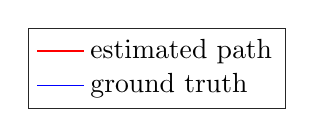
\begin{tikzpicture}

\begin{axis}[%
width=0.951\figurewidth,
height=\figureheight,
at={(0\figurewidth,0\figureheight)},
scale only axis,
xmin=-326.133610460546,
xmax=302.990672157041,
ymin=-17.60491,
ymax=478.5915,
axis background/.style={fill=white},
legend style={legend cell align=left, align=left, draw=white!15!black}
]
\addplot [color=red, forget plot]
  table[row sep=crcr]{%
-0.0254918464849211	1.53029535298794\\
-0.0249375910517428	1.94734709129581\\
-0.0603236978854961	2.65467351088822\\
-0.0898810439678936	3.26129873758476\\
-0.122075910017149	3.77863002775827\\
-0.159570842977669	5.84214038823241\\
-0.16292475786949	7.0836905643616\\
-0.345776789656112	7.86663308840102\\
-0.27491593989267	8.64211113561682\\
-0.309598017914873	9.85377995390277\\
-0.277110669964546	10.8074353831312\\
-0.341823185026675	11.5749687634724\\
-0.217613495970221	12.8917284400095\\
-0.0592983580678572	14.5355139663008\\
-0.180912031378883	15.8651152558168\\
-1.26697074582979	18.3123350977835\\
-1.99632227513441	20.7279831935775\\
-1.84207392672155	21.2111290079799\\
-1.99288467857056	20.9603081203128\\
-2.43488020065001	23.6076482593938\\
-3.32814670014799	26.4212881100612\\
-3.41386831765519	27.9866495815779\\
-3.26771019182501	28.8006409927994\\
-1.620921197859	28.8478264025535\\
-1.01053561934922	30.1804555073533\\
-1.36990364301468	31.8801443840733\\
-1.68848635244443	33.0028846017483\\
-2.957683281011	34.549655907193\\
-1.93727364960529	35.2393504197716\\
-0.514689122519029	36.4952841572078\\
-2.41146050849461	37.8049416860848\\
-2.71386629862038	38.9356379876211\\
-2.5836966234896	40.2781502625555\\
-2.63882225372063	41.1601732819549\\
-2.7230539754266	42.7122931760083\\
-3.11906810826344	44.0178342459916\\
-3.5576739125108	45.3115982132388\\
-3.73668414556942	46.8983634413674\\
-3.42579027512101	47.4997854636121\\
-3.37452161806168	48.4033528851216\\
-2.99163928820322	49.6636239919109\\
-3.10320887584081	50.7018844714724\\
-3.0464797680176	52.1475222356591\\
-3.35653817862564	52.1640341844091\\
-3.40230080816271	52.6660400071882\\
-3.54859891943742	53.5245721842838\\
-3.85443388284758	54.323034107439\\
-4.27092801067289	55.4027333112678\\
-3.97498857188129	55.7474911357893\\
-4.22640325846508	56.807195966801\\
-4.51433986168065	57.6606194774688\\
-4.45132591225925	58.2961906821192\\
-3.87087302966426	58.9926053369621\\
-3.87072061323249	59.9732514095607\\
-4.12549889751349	60.0402193663624\\
-4.17340173135913	60.7456678843814\\
-4.12893217891143	61.1970095247609\\
-4.12533541504708	61.6150479715717\\
-4.36319411086895	62.0515472529026\\
-4.23740722860777	62.8444458014122\\
-4.51626044562072	63.1617794277363\\
-4.74172961135334	63.71782329942\\
-4.97379009828556	64.2167702806049\\
-4.93061997905132	64.4311587159421\\
-5.23783523344155	64.5675148118491\\
-5.19475716845265	64.8938107140529\\
-4.67515401799115	65.7924239026028\\
-4.82628344330113	66.2844439179433\\
-4.9776538232629	66.6504952760732\\
-5.31565671921746	67.1836152214808\\
-5.34808236169056	67.4940749889046\\
-5.52470833181015	68.0121192714174\\
-5.4325465157858	68.3096344099097\\
-5.55867614573155	68.8287307904144\\
-5.88037145530012	69.3203977107901\\
-5.91546037096899	69.5711686151296\\
-6.08013796305789	69.9628565133067\\
-6.14556482172951	70.0334308787011\\
-6.15402724565322	70.7374385452911\\
-6.1460508720291	71.331972565127\\
-6.328808074714	71.9296173363728\\
-6.35929505314514	71.9173406638082\\
-6.50422911477137	72.1784273380596\\
-6.48712747306594	72.1900835093829\\
-6.53615775206799	72.6287951737309\\
-6.61322228136018	72.5698976819463\\
-6.6359028941971	72.7247640830418\\
-6.63443813278765	72.827386557307\\
-6.63304305340155	72.7849449423394\\
-6.59914635250929	72.8397191729225\\
-6.63099988813093	72.8502703609318\\
-6.62598394124391	72.8839815830864\\
-6.677222405543	72.990222162353\\
-6.69606306876206	73.1023825882362\\
-6.67947403851695	73.1018321192448\\
-6.66964521152038	73.0849083191595\\
-6.71753454770595	73.2479563214644\\
-6.68329511014403	73.2136288221336\\
-6.73156605219733	73.3523697969232\\
-5.74916022487019	74.8576967814507\\
-4.98596335328253	75.7765272109256\\
-4.43775978820118	76.3360490216935\\
-4.0351963913887	77.1432020353311\\
-3.31168111220858	78.0935985551581\\
-2.57500295189668	78.5395817761753\\
-1.75831772445147	79.1727569746753\\
-0.832372415140044	80.0561318694447\\
0.165432628004261	80.9139244863526\\
2.01907230576175	81.4745534459841\\
3.03787339267238	81.941688130993\\
3.78789086121179	81.9303354908679\\
4.71875426558578	81.9083376711678\\
5.78475750137049	82.1404701329294\\
6.60049592733277	82.2386633234372\\
7.55069181843053	82.1705053819\\
9.18940635647107	82.5998881880914\\
7.79304789579438	82.3028385882826\\
8.31752099758972	82.0297188638339\\
8.46510269461545	82.1474546099009\\
8.92997122166296	81.9975240011056\\
8.72142415686466	82.1328916507775\\
9.62952123553625	82.35126669387\\
10.4428547717025	81.7225762020355\\
10.5299924409937	81.9554276383626\\
11.1340486098493	81.9050518843603\\
11.5160997827738	82.0612281350407\\
12.2594588259065	81.835334632617\\
12.3842394637717	81.9428961031885\\
12.4818562140108	81.7950071519373\\
13.1501427687121	81.7332779817331\\
13.4321889232477	81.7065373136024\\
13.5792795550453	81.5447206480089\\
14.3849820421582	81.6817796087256\\
14.6707460261462	81.6564011663676\\
15.387556467747	81.6302305944835\\
15.4036264863747	81.4691316519079\\
15.901957749803	81.4784151382603\\
16.2496710930681	81.3085331013827\\
16.7706031899464	81.3848422837381\\
17.2506820326831	81.2216128634827\\
17.5420899299026	81.2295689563559\\
18.2429412493675	80.9353345131872\\
18.9092503287814	80.975881509787\\
19.3062861034766	81.0781914443557\\
19.3127546717529	80.9762082267525\\
19.7313263193219	80.8288055072149\\
20.1281292873987	80.8231780164422\\
20.5014009404501	80.7553345527887\\
20.9612097591178	80.724608480742\\
21.144835486253	80.7738315142502\\
21.6856651911413	80.7143847422054\\
22.3622936571346	80.6394818706931\\
22.7506957542649	80.5950105855102\\
23.1307233875676	80.5231776478185\\
23.9196728507744	80.4114076741925\\
23.5649148204362	80.4630173661273\\
23.8468922067825	80.4214741927698\\
24.1645155468505	80.3934453896117\\
24.7700216475903	80.311962790901\\
25.1026903198501	80.2327290500051\\
25.3452871712123	80.2184045541649\\
25.7084744721147	80.0993975123769\\
25.9762818582351	80.0361410422209\\
27.8471866730257	79.6327428569191\\
28.5665207409481	79.6397780304731\\
29.3706760454403	79.4845412413973\\
29.5131424231395	79.2054605096551\\
29.8712925651193	79.1636295304659\\
30.78572174128	79.1032161488192\\
30.7494125908544	78.9734183358357\\
31.0689711140398	78.8581495956416\\
31.6429288794151	78.7407207121995\\
32.2531780740753	78.5592455938852\\
32.3433431784366	78.540363958724\\
33.0194843461616	78.412748459995\\
33.448015354965	78.2948541133615\\
33.2545897991583	78.2101566022689\\
33.7027662042132	78.0766153094535\\
34.000903983259	77.9815387258325\\
34.5577628820091	77.9018086272159\\
34.7860146798725	77.8821206641104\\
34.8701692473609	77.8150543776238\\
35.1753777754168	77.7400843195754\\
35.2951791891894	77.6574576574895\\
35.5254230531255	77.6149095078541\\
35.7513394555345	77.5822724039432\\
35.931804178265	77.510737724749\\
36.1386117030041	77.5999232664415\\
36.305435898856	77.5258353963908\\
36.5685398125925	77.5162600132465\\
36.8314269959987	77.5488092312873\\
37.0028201777755	77.5545693355\\
37.078609155348	77.5291100691133\\
37.1112445133585	77.5626524408347\\
37.7140446533923	78.1298258000892\\
39.0226936351646	78.478028339954\\
40.0631847221038	78.9320014992913\\
41.1931123550825	79.4661719508874\\
41.7415486250996	80.2580050936122\\
42.4048102152318	80.6182828937917\\
42.8874442208446	81.3354842647558\\
43.4063508805456	81.9061523279002\\
43.8637544689313	82.5468578458166\\
44.2219188036745	83.3305912093998\\
44.6984090619231	84.186883159669\\
45.0731293816831	84.7732420681804\\
45.1718017243228	85.7074001071109\\
45.4363478246522	86.2481542416149\\
45.7404816064923	87.0118713020081\\
46.0570211146635	87.3820347293203\\
45.8965337706401	87.1654040422665\\
46.2213194143059	87.9160220120286\\
46.4738068508331	88.0872372369035\\
46.3065209081047	88.7634327596495\\
46.4366982832061	89.1702923387284\\
46.6585067458771	89.6997025690013\\
46.7808009608587	90.0834144908274\\
47.3914049395722	90.5988945779756\\
47.3636284416625	90.8286295608408\\
47.2265269009887	90.2143994556028\\
47.717578659049	91.3091794373966\\
47.8500424255384	91.7210507845807\\
47.7293051526632	91.8055094095902\\
47.640832921726	92.6627964301926\\
48.4532520164321	93.0136712508394\\
48.2400085602705	93.451291387018\\
48.7062298458964	93.5749720820282\\
48.7578683816512	94.3337817657926\\
48.9176626931242	94.5661619819297\\
49.0833941050341	95.041602011071\\
48.9404409462835	94.8860811961652\\
49.2541499450167	95.4141855326174\\
49.4966650270903	95.6436190171969\\
49.623632405671	96.1600777931367\\
49.5344735387433	96.7208701790154\\
49.7608266983671	97.0498924950989\\
49.7867289270388	96.8886328998434\\
50.0361596849583	97.1938059804105\\
50.1516872721954	97.5284099064471\\
50.3114640239943	98.1312987140743\\
50.4881558028099	98.6888951391392\\
50.6735948549936	98.9514355191266\\
50.8338738897649	99.1888832442082\\
50.9749524872735	99.3790873433498\\
51.173853550999	99.5441269463878\\
51.274874940414	99.731659637568\\
51.5147621379885	100.400677568163\\
51.6431013735094	100.666787735751\\
51.7468736122773	101.035816553951\\
51.9246036035865	101.388311800899\\
52.0061329537239	101.617937033054\\
52.2564893913523	102.036792706017\\
52.3633982028635	102.245795643879\\
52.5105372269858	102.512294243641\\
52.6584143865775	102.64885513828\\
52.7925818273266	103.043485751074\\
52.8579132078163	103.165924407148\\
53.0079820406809	103.390920440981\\
53.1038244667886	103.72214890501\\
53.2132918321541	104.078019863707\\
53.2703656826956	104.260392151337\\
53.3539538903897	104.414219794868\\
53.4269162582695	104.70656092463\\
53.6082556220211	104.842142674817\\
53.7581103851577	105.047089704945\\
53.8263368003714	105.402846650693\\
54.0121538902149	105.523955070453\\
54.0980954258794	105.685904784581\\
54.3412550062454	105.965861319593\\
54.7104888921945	106.109484785291\\
54.7178580688169	106.471921428318\\
55.0856951814603	106.57391256521\\
55.5568975538975	108.300767297303\\
55.8673994603171	109.295263265782\\
56.0746751747559	109.787000189357\\
56.1484614961019	110.297945175921\\
56.399957004125	111.153774229954\\
56.4867841257466	111.553112323513\\
56.4045163510286	112.14480132409\\
56.3431219818062	112.799200844566\\
56.8104375436088	114.823659417198\\
57.0851662916506	115.683343431339\\
57.2644066720422	116.946405244776\\
57.2743106434736	117.80172121014\\
57.5748946381337	119.061412673349\\
57.5091470864185	119.686271048881\\
58.2095110964307	120.423364521672\\
57.9185881397623	121.700980032441\\
58.4577709971528	122.843312336497\\
58.537027542623	123.252505452575\\
58.8484483500288	124.099676852421\\
59.1928528465394	124.56585624148\\
59.4790781063918	125.67175425309\\
59.7688817856568	126.405777528763\\
59.8062976015062	127.15612090542\\
60.0438999184809	128.374284309363\\
59.8243082383549	128.581654793278\\
59.7527525143428	129.600574617913\\
60.1092031610225	130.244486531151\\
60.2960259967395	130.982000286757\\
60.3221150114104	131.721004376834\\
60.5206128308354	133.646700950585\\
60.5364210965518	135.016293900279\\
60.7235203620208	136.793671231076\\
60.7713432026474	137.657583032728\\
60.8310382545652	138.594310635866\\
60.7529997379493	139.6807143518\\
60.9417215781221	140.121526154869\\
60.9620837640592	141.130146883736\\
60.8739323381193	141.914874196497\\
60.8271528376307	142.873829131889\\
60.865644365926	143.460001342915\\
60.9222558029635	144.098262655698\\
61.117574125958	144.844205523261\\
61.2719254849057	145.391099643084\\
60.9277189868364	146.558639804799\\
60.8368628934674	148.021070340742\\
60.8991573216548	148.82931283865\\
60.8347738926756	149.421854335248\\
60.4513603060383	151.512919254189\\
60.5934063589759	152.609382361094\\
60.4509927225821	152.714768097186\\
60.4658444409244	153.846265494586\\
60.3866604032632	154.441735998167\\
60.3969587658767	155.269374499588\\
60.415329501319	156.062569892952\\
60.2417822434478	156.390003029709\\
60.294726780757	157.289081018436\\
59.9764585085438	158.295185420979\\
59.9759795756181	160.182878788607\\
59.7691192626721	160.920512964375\\
59.7247229921041	161.669115786819\\
59.7923034587661	162.169043755827\\
60.0435099009338	162.62996373967\\
59.8655608913164	163.728016200874\\
59.76426217954	164.619714155139\\
59.6756670984734	164.526358228161\\
59.6109670024469	165.291652641248\\
59.7328261800477	165.351196267701\\
59.7297072276716	165.859759789378\\
59.7150599666397	166.319431662871\\
59.7343281276525	167.085891526232\\
59.7611524688876	167.240009569929\\
59.7107004114382	167.96525218535\\
59.4407684063036	167.641608622908\\
59.634125617127	168.168869583705\\
59.9884467741038	168.496233188886\\
59.8860400305554	168.895609804142\\
59.4647096657804	169.602503448262\\
59.5211765900685	170.135306695873\\
59.4276354116568	170.554135389576\\
59.3538829943736	171.049256417134\\
59.3553479313054	171.146876675915\\
59.3570823870751	171.488528396088\\
59.3496936302469	171.755578492643\\
59.3496674944258	171.939810998851\\
59.358830959232	172.048755507418\\
59.3197345676849	172.27148372958\\
59.3215253935262	172.423647834218\\
59.3183657136134	172.51893826744\\
59.3216558269431	172.59932443784\\
59.3281827761251	172.808205494299\\
59.6034235616614	174.743134462683\\
59.5456523730993	175.539087287724\\
59.4140774447768	175.102072459793\\
59.4970388158576	175.258656848367\\
59.4576717501172	175.536637762001\\
59.4904226725158	175.898720199413\\
59.55830637525	176.324468398914\\
59.5346831547861	176.497239063372\\
59.5637717272731	176.875511614279\\
59.5817492627266	177.083108081822\\
59.5903244465374	177.176919243799\\
59.6470978756398	177.422472770544\\
59.705046663632	177.785236566059\\
59.6529916039159	177.715563065947\\
59.6905482305924	178.182512076715\\
59.6796524382431	178.510376179112\\
59.6862663797934	178.775275858893\\
59.6817221099888	178.940607768172\\
59.6753220830399	179.356937518334\\
59.5592750857287	179.682735376786\\
59.5347610850979	179.89224188034\\
59.614889376402	179.975756493434\\
59.5757936126343	180.152558089843\\
59.6337517443448	180.346532513138\\
59.6856167511302	180.479848322005\\
59.5168251104199	180.868045315986\\
59.5492300030534	181.191521476844\\
59.5580716305347	181.259835959325\\
59.5413986866597	181.396464604533\\
59.6367421671284	181.474658626172\\
59.6193165860309	181.546632190516\\
59.5673270522548	181.672124178715\\
59.6238442739857	181.793248479743\\
59.6226514104726	181.907128464503\\
59.6384244590302	181.986764047142\\
59.6188692117161	182.073693540248\\
59.5595584069414	182.163920284658\\
59.5632101926767	182.234094969913\\
59.5131467405562	182.252403882491\\
59.5397136152566	182.199215893866\\
59.5210791058123	182.257304043564\\
59.3911564963095	182.33742157826\\
59.3147214159076	182.390957634294\\
59.3335080803308	182.449718813748\\
59.266984446761	182.509491961506\\
59.1516116460686	182.516893225503\\
59.0394367557121	182.595833211739\\
58.9547800094417	182.662740359614\\
58.9090709459745	182.693560889666\\
58.7890538635293	182.808878616883\\
58.8136254663913	182.785413118039\\
58.8204132219171	182.794181951592\\
58.8079286225571	182.803536162117\\
58.7679920810716	182.829193777072\\
58.7202419814376	182.844970078658\\
58.656767883704	182.869884420455\\
58.6390985803914	182.864646811355\\
58.5788115006392	182.891063478687\\
58.5179632795888	182.928115661594\\
58.5067257532484	182.961100202163\\
58.4559498079406	182.979105544387\\
58.3972692896788	183.015473450295\\
58.3562568572456	183.02141275462\\
58.3083049993463	183.046882077481\\
58.2580233262766	183.096498568932\\
58.2084541175408	183.116158338559\\
58.1724347427656	183.133139301638\\
58.1336133013281	183.134415104081\\
58.0772245636923	183.187010973838\\
58.0147932146204	183.178406137348\\
57.9744850144966	183.175192985046\\
57.9245583116846	183.20367015069\\
56.1423772572669	183.283334610768\\
55.0759509673546	183.319409179976\\
54.1648847643883	183.526017430069\\
53.9681363878199	183.214710063521\\
52.4541027205024	183.439284256777\\
51.8021792473829	183.585321683964\\
50.9998251023726	183.525740301558\\
50.3772479503727	183.572319587374\\
49.0585592500209	183.840062661996\\
49.060492488932	184.161287245795\\
48.1230600931	184.198801749217\\
47.1024506187664	184.337698851144\\
46.2393207467898	184.402671997887\\
45.4747710043928	184.505727426855\\
44.731785657727	184.652837105292\\
44.0862678261191	184.681229095893\\
42.9774897849456	184.79244694102\\
41.4202980943571	184.607943461226\\
40.896253209493	184.550670399857\\
40.3909450934301	184.385620687242\\
39.9266142577062	184.352292406955\\
39.1663283272719	184.176871897265\\
38.2365489125349	184.380209555892\\
37.8588033570567	184.390025726584\\
36.8522542507326	184.489441341296\\
35.8733693801279	184.432842478328\\
35.1855194164048	184.242101040757\\
34.8978273181622	184.347125148305\\
34.0783318101893	184.378207211825\\
34.2245692380846	184.429975599638\\
33.6413088678831	184.4085253844\\
33.3540029067821	184.300502522713\\
32.7894365932384	184.235202803213\\
32.4830220808442	184.121270948495\\
32.3020019651882	184.140183456111\\
31.640297607302	184.110135312948\\
31.1579798194393	184.026709212543\\
31.023280374801	184.385754449169\\
30.5965558955248	184.125582611666\\
30.0629365310112	184.122653374302\\
29.7204614872029	184.01370614265\\
29.3189518891985	183.820174062197\\
28.9617893232784	183.852097466715\\
28.6104139764052	183.692817899858\\
28.0899614717814	183.66293071392\\
27.8244876074492	183.562111676699\\
27.4103561798431	183.403067593153\\
26.9989540299813	183.377011414264\\
26.9050233103113	183.665218985696\\
26.4047007437558	183.421269081078\\
25.8356512818452	183.194244975614\\
25.5284707289566	183.155112344951\\
25.1283612561322	183.051783379607\\
23.4877873701655	183.04407895534\\
22.7775602649169	183.042859130632\\
22.2093701622086	182.902667718048\\
21.6087750943676	182.950469010411\\
20.6769076718578	183.010709156085\\
20.3755334904599	183.175533193215\\
19.6235376637793	183.206468588444\\
19.2395756001072	183.207278898757\\
18.7841733949186	183.352344774804\\
18.23054973662	183.206354177479\\
17.7362316780864	183.322294325599\\
17.4350221766438	183.713378767133\\
17.0297935071111	183.631402672629\\
16.8245552703425	183.926898859322\\
16.3631828657795	184.122462435523\\
16.0872362821424	184.11921540653\\
15.7543110849923	184.1594251089\\
15.464449827911	184.178915848841\\
15.1232348995428	183.943131951397\\
14.7970525770037	183.978775338301\\
14.5292615999103	184.180055447564\\
14.4142668383255	184.173446768211\\
14.0357364355367	184.205189218846\\
13.9212363751845	184.243076043493\\
13.9532710611444	184.296841790495\\
13.8012259521892	184.378771514476\\
13.4626052469625	184.317909038324\\
13.5053134734772	184.412063543674\\
13.4281150078388	184.39582031143\\
13.2623272073817	184.278256197803\\
13.261549276469	184.328956775609\\
13.2556839909804	184.360885886702\\
13.2161820100243	184.351706201258\\
13.1795037962938	184.404256098137\\
13.1778666593255	184.383915701078\\
13.1622975264406	184.395005352988\\
13.1644003925405	184.38229677913\\
13.1164116538569	184.387445357888\\
13.1486520990252	184.385873409739\\
13.163329976223	184.394291599793\\
13.1752494089085	184.380512823397\\
13.173314740378	184.405276339304\\
13.1447806688955	184.373956578639\\
13.1492435704402	184.379551068165\\
13.136859273752	184.393596335987\\
13.1539817759598	184.377695161448\\
13.1491105378692	184.381105178826\\
13.1648502604557	184.369864309074\\
13.1662066079309	184.371002034705\\
13.1581527986809	184.371772428388\\
13.1617769082975	184.370849061909\\
13.161713905888	184.370492615336\\
13.1561224943931	184.372277661299\\
13.1848648192474	184.364105823053\\
12.6522976887069	183.73662161087\\
12.7000570322595	183.474261776714\\
12.345205196928	183.778152681806\\
11.7548755724234	184.594993214024\\
11.6348635709837	184.310941028938\\
11.1531559638741	184.489121667325\\
10.9308537673685	184.755930705704\\
11.0278486024333	183.782576276662\\
10.8029503724915	183.832140316844\\
10.2475621782028	184.148317974667\\
9.9494157165913	184.236183030293\\
9.8812610122607	184.210927427721\\
9.46925135535171	184.516165731852\\
8.76006564948287	184.860526623167\\
8.4599224438988	185.008770183866\\
8.44907447504853	184.896577004155\\
7.71621058541695	185.740297552297\\
7.41273032037312	185.794512308762\\
6.9095458774069	186.204023867148\\
6.75120974794374	186.850487522282\\
6.14679295989508	186.918685931456\\
5.59730534709833	187.113531509051\\
5.08169070244708	187.652240247498\\
4.7121298496674	188.099980367826\\
4.17880859938765	188.678590920072\\
3.67278796233225	189.040605379242\\
3.74773829020509	189.989328981472\\
3.52735216835979	190.177181798304\\
3.13500755579086	190.689274702827\\
3.65513751830715	191.485769655382\\
2.9733609309834	192.192240921153\\
2.86431050313467	193.385452656526\\
2.74613790653906	194.027171572758\\
2.42200416981464	195.236873491357\\
2.59046170435565	195.295994436998\\
2.42016618070335	195.918221496054\\
2.8060517820064	196.807773620133\\
1.99457206660195	198.443261720685\\
2.61692138879642	199.67110679594\\
2.68042305491054	200.508847001397\\
2.56597280500196	199.844439634594\\
2.43106842843965	200.827531827684\\
2.36180071380823	201.683774835402\\
2.47526776590718	201.801844480794\\
2.43485134127791	202.948778198456\\
2.26149326270073	203.361238146291\\
2.40369219305361	204.036607636671\\
2.19746353982454	204.560182495754\\
2.04183371630161	205.185665105598\\
1.91079396920826	205.982234694303\\
1.93028503749185	206.203378073365\\
1.83471546633074	206.793675980463\\
1.78623016107632	207.189695802168\\
1.71989906739976	207.522828242109\\
1.60362310880505	207.876477980968\\
1.4741156171317	208.237696860463\\
1.81278484103078	210.181615174642\\
1.95967958919012	211.248836774986\\
2.26981335325668	211.999119734909\\
2.26868240545766	213.016315980298\\
2.42571157365921	214.424409475541\\
2.35948177930214	215.815516768664\\
2.18410309285501	216.964702229816\\
2.29380151818637	217.471821217596\\
2.4258955422234	218.488047704461\\
2.4359178450232	219.371638384033\\
2.85359164981374	220.506832722578\\
3.05426238028021	221.649256009545\\
2.90515872148854	222.741095355119\\
2.87432461592194	224.181819890834\\
3.27614316412384	226.072274216382\\
2.98574606623752	227.05320677208\\
2.91472791758863	227.530662837713\\
3.28631478503829	228.939515382434\\
3.40895783013496	229.550937176239\\
3.51630396570227	230.458391272202\\
3.66118850688889	231.547129384246\\
3.64426841144758	232.232078823238\\
3.86764892265458	233.063620976214\\
3.89725179264675	233.760945836218\\
4.00630176819153	234.496575907511\\
4.22847000563517	235.389672139322\\
4.34654011556515	235.807390349054\\
4.73081267072256	237.582028319241\\
5.01642454178728	238.575664208767\\
5.04818092659095	238.77536394743\\
5.13764317773981	239.420119681382\\
5.1783065966476	239.857746081319\\
5.16765021502875	240.648640949052\\
5.1756702803605	240.731633532029\\
5.30181954688528	241.329522541618\\
5.21366910618884	241.550853610451\\
5.21626317783681	242.032937508895\\
5.10027311172254	242.355261091628\\
5.24339110700473	242.444449428145\\
5.3456269227876	242.785933345209\\
5.39063361110616	243.107224116003\\
5.16882323584604	243.392455988195\\
5.06195377133296	243.645530902281\\
5.77349906294497	245.447571102233\\
6.12181791365101	246.489886035378\\
6.49092986853619	247.322605868297\\
6.86336397918412	248.294088610777\\
7.22753835642201	248.957485202488\\
7.62273019684161	249.715343577061\\
7.97410136085511	250.688617407164\\
8.33424046437679	251.475957428954\\
8.87290912932699	252.532537565792\\
9.21464152516252	253.361491594413\\
9.37412608073542	254.029444510883\\
9.63272264238788	254.56880639033\\
10.1092148179902	255.635282931332\\
10.3528958555751	256.243477008611\\
11.2246143458406	257.745345900288\\
11.727525315841	258.612650804202\\
12.1552506530377	259.472749206214\\
12.8162454756073	261.137763155593\\
13.2356176858853	262.204912436007\\
13.5938352447748	262.976667899981\\
13.9211838025426	264.262857931221\\
14.5788192585701	265.38789140253\\
14.8823005593628	266.45662882966\\
15.1041811070841	267.377523785985\\
15.444610936724	268.32779849705\\
15.410335617981	269.150416422174\\
16.0833437218745	270.999522639039\\
16.4134556880758	271.930957678277\\
16.7791355814524	272.993349030161\\
17.1823644777274	273.693762356396\\
17.8671649599833	275.508085121917\\
18.1857348754236	276.282901624096\\
18.2776875276326	277.74533420464\\
18.7015579537899	278.543364030728\\
18.8180408974974	279.659134244501\\
19.221999783895	280.639613940235\\
19.607646456117	281.928251169042\\
19.5666714246325	282.456268177206\\
19.647432881872	283.276850188455\\
19.7022825320953	284.035213183811\\
19.7035672266372	284.857546888977\\
19.9453127977096	285.382915990202\\
20.371025374387	285.835397218776\\
20.5306324881841	286.251527298036\\
20.7933421676451	287.037793152693\\
21.0009902932991	287.89375159755\\
21.2265169414746	288.392671874244\\
21.479127051484	289.000951292358\\
21.7777032216287	289.704262300904\\
21.943837731553	290.675060350659\\
22.2119270892377	291.534340553632\\
22.1587322632875	291.85554291316\\
22.4062758402464	292.683600369947\\
22.5369845270625	292.678735898307\\
22.7671743043204	293.008334569001\\
22.8199522231628	293.658609540736\\
23.0873953375229	294.30403110232\\
23.3046228207672	294.535663431176\\
23.2552973887695	295.09398956614\\
23.4895286035062	295.406067832158\\
23.4612022898545	295.553275329464\\
23.5298241326255	295.892628581203\\
23.5500535287344	296.013519212675\\
23.5401961957187	296.122205460085\\
23.6072013720259	296.14674265573\\
23.6209289876438	296.223255193307\\
23.6366311437099	296.455570091941\\
23.6005928616927	296.38017038791\\
23.5916209493248	296.410774888066\\
23.6165064149772	296.438404870384\\
23.6117510250539	296.305047975966\\
23.6108002410788	296.297942255874\\
23.595781955602	296.232990042938\\
23.5929572877563	296.192610344715\\
23.574458590281	296.13018206209\\
22.9488584393414	297.513551584578\\
22.8216451584009	298.307639100467\\
22.1392152329466	298.881241723663\\
21.68700741702	299.634091229204\\
21.0873365853499	299.869963792016\\
20.4258628445185	301.227669431162\\
20.2360311788066	301.647040766348\\
18.964472891903	302.412636853062\\
18.290182832503	302.539895824066\\
17.8700263083068	302.930969354233\\
16.9710512072508	303.183735371103\\
16.6209036483586	303.641067130349\\
15.0578279822163	303.961209930646\\
14.3011206295675	304.428249955449\\
13.2168583791909	304.408530738501\\
12.7973923288869	304.478835734603\\
12.5681920973157	304.36131005668\\
11.8717506660714	304.506830753451\\
11.540060308396	304.40251246754\\
10.7983063176871	304.533126292615\\
10.81443584271	304.487770049368\\
9.98950297350394	304.734105805977\\
9.53477840680498	304.850099661466\\
9.1428206687778	305.054615656651\\
8.79687530856623	305.243513341745\\
8.16345276458071	305.516543179345\\
7.79340804748047	305.616592505709\\
7.46317294045154	305.626416299299\\
6.77955445661987	305.760327413064\\
6.07559067510214	306.165208228471\\
5.63298914498354	306.119463571366\\
5.10530280561759	306.167932212638\\
3.50846918243129	306.693561550124\\
2.79112392841185	306.806831198753\\
2.13325255028205	307.122356382722\\
0.532486454828418	307.616093612101\\
0.0713091566940755	307.760505540975\\
-0.440284598862597	308.027713501832\\
-1.85692326789706	308.504315366516\\
-3.0220988161549	308.635873313937\\
-3.85332147086734	308.965808666582\\
-4.92817228876401	309.281638869758\\
-5.61780211598453	309.339873446184\\
-6.39733675017839	309.481796387154\\
-6.92225294603483	309.663852540937\\
-7.3179630243356	309.801933960105\\
-7.36155780766051	310.045030336111\\
-7.97958612886192	310.267613612792\\
-8.7548384215207	310.263531378416\\
-8.66717180077974	310.348752296061\\
-8.9262080681754	310.377298577379\\
-9.3210812368515	310.589422854776\\
-10.027891983154	310.916858821722\\
-10.3066263780137	311.199927469676\\
-10.2364539187342	311.03226619783\\
-11.8091338075766	311.284832824698\\
-12.2754975506547	311.305890233085\\
-13.0991390600251	311.766044956694\\
-13.4824696891787	312.029609501167\\
-14.2139712107997	311.938223788202\\
-14.6373016964595	312.039375896455\\
-15.1846268524205	312.2257258256\\
-15.6710475621027	312.286813256877\\
-16.25956457169	312.544968869679\\
-16.6624688765141	312.986968249209\\
-17.3026005196284	313.077846825637\\
-18.0973994592544	313.869891130455\\
-18.5334129359234	313.936736444334\\
-18.4392962772833	314.07358130524\\
-19.0053093945902	314.946844250767\\
-19.6015718514847	315.026316319144\\
-19.998635376012	314.793914550077\\
-19.9192520271521	315.37140037174\\
-20.7685567481013	315.396573353689\\
-20.9839619650651	315.527030658799\\
-21.2819113847184	315.725633261436\\
-21.6864307899352	315.713506141714\\
-22.2154508670534	315.992768930537\\
-22.6645583018319	315.956486789564\\
-23.1733225667174	315.969396834518\\
-23.0778406775508	316.342463815643\\
-23.8905718996308	316.298576124429\\
-24.014594834156	316.328392780981\\
-24.4719100193317	316.44226008668\\
-24.7957915329538	316.611861907387\\
-25.3670150125555	316.749441886213\\
-25.6981743422059	316.857893917178\\
-25.9768804223722	316.92506396512\\
-26.0745569978171	316.950211073102\\
-26.3151770160126	317.041214666698\\
-26.6067928007891	317.028665165199\\
-26.9089978459774	316.825212986564\\
-27.0904105035401	316.824311995475\\
-27.5132871862149	316.657101825775\\
-27.5366737698789	316.884778228695\\
-27.9532758867494	316.764709194588\\
-28.1010928684258	316.930686685425\\
-28.3557795117554	316.87304361641\\
-28.6646885195009	316.813729692975\\
-28.9928682606587	316.783765094685\\
-29.3397946060269	316.670835338711\\
-29.5823158553062	316.729721417602\\
-29.5993391608501	316.900586585241\\
-29.8400393927703	316.831865794656\\
-30.290536465674	317.087611166175\\
-31.0401603414646	317.470443108997\\
-32.464068554313	317.53973935929\\
-33.1089563269751	317.558617259501\\
-33.7023390182299	317.728253732394\\
-34.3273687817922	317.654583536761\\
-34.7460455443326	317.792609589787\\
-35.50472066392	318.097741644225\\
-36.1249359875149	318.243042491979\\
-37.1113958364566	318.528441360581\\
-37.7248746903805	318.997342828775\\
-38.451018598279	318.975144456613\\
-39.1032857021091	319.367602917834\\
-39.7399173530366	319.419145339896\\
-40.3955047976064	319.366118900283\\
-40.7190285576429	319.601544336017\\
-41.3651098585153	319.605236308698\\
-41.9717712731981	319.546278107535\\
-42.6307032031486	320.037025611631\\
-43.3862940414625	320.154883614419\\
-43.6378954651299	320.171119790011\\
-44.3433610181346	320.250620625285\\
-44.8483095089634	320.168450730246\\
-45.4045674778744	320.102238476281\\
-46.0050218743012	320.258313605069\\
-46.98049312579	320.667547198419\\
-47.3321330293453	320.348491243427\\
-48.7122968601904	320.529621077991\\
-49.418740675701	320.496454209439\\
-50.3578365592231	320.64982260259\\
-50.9208825196296	320.538183026815\\
-51.6777885567466	320.663003186544\\
-52.289917033537	320.597354813711\\
-53.87238999796	320.682540867696\\
-54.704939949552	320.633607132348\\
-55.4094564168921	320.789875004832\\
-56.9914261204273	320.845961502324\\
-57.4123306932968	320.758413577392\\
-57.676729259607	320.951710524189\\
-59.1334403206073	320.928392891428\\
-60.0158371639667	320.913465759189\\
-60.2881280724558	320.969169963936\\
-61.1137879707161	321.554942757028\\
-61.4770585957186	321.487892331777\\
-61.7455751151043	321.520524743632\\
-62.2494774403446	321.568445490927\\
-62.5313311509598	321.445023586837\\
-63.6232834148889	322.04523472927\\
-64.0549952618846	322.196429034627\\
-64.7404498268431	322.256381064037\\
-65.387223177527	322.59880022078\\
-65.9312891456674	322.533268980704\\
-67.3707837943606	322.315473909943\\
-68.1152389107837	322.330361650441\\
-68.8832691507362	322.394703937506\\
-69.3755018650706	322.281683726983\\
-70.1451986174682	322.211753015592\\
-70.9526330088287	321.95665022527\\
-71.7786857841303	322.213503158367\\
-72.0227970298683	322.24888646721\\
-72.9745545971479	322.469747341054\\
-73.2848546936096	322.542747282974\\
-73.8967088709999	322.410727523674\\
-73.8390799788937	321.847075271148\\
-74.4278362415457	322.165801369496\\
-74.8264216461862	322.053884835782\\
-75.5817114951405	321.864705247303\\
-76.6020561170843	321.803496060704\\
-77.2011372589449	321.840475962899\\
-77.9725835930079	321.878526131062\\
-78.7072424745332	321.753297022006\\
-79.3776185847263	321.556913352276\\
-79.900346485615	321.456350481903\\
-80.6407328213149	321.333829516657\\
-81.1488122500518	321.508924635974\\
-81.5301931351267	321.57413610244\\
-82.3414627431139	321.386500250169\\
-82.8739001879264	321.207613640895\\
-83.4313861692684	321.236892463738\\
-84.2518943842188	320.666453297985\\
-84.6503265032367	320.790580093863\\
-85.3309200453473	320.327590533093\\
-86.1087580369316	320.005030891002\\
-86.2764240890651	320.242697125587\\
-86.5408726954713	320.140687551868\\
-87.1619789267885	319.784296828144\\
-87.8474168277385	318.947127225515\\
-88.3726009425346	318.497745107585\\
-88.9253193531665	317.976387482342\\
-89.5354359251712	317.596334642859\\
-89.9518564032857	317.057891508834\\
-90.8436166311986	316.395286077754\\
-91.4197845038835	315.74146029828\\
-91.4988649685286	315.278165919325\\
-92.2366241772499	314.27820582081\\
-92.5925395379685	313.545415720678\\
-93.1977240970668	312.346538418796\\
-93.3671153143451	311.833936705211\\
-93.8933885150585	310.685416819795\\
-93.9446444368903	309.87765454689\\
-94.2001387941639	308.994547916272\\
-94.2552966689455	308.082743059\\
-94.1165339324721	307.186525756743\\
-94.1724734649761	306.306731317866\\
-94.358413709005	305.142788871709\\
-94.7631958788326	304.244479852602\\
-93.9970956915029	303.115491613402\\
-94.17469265039	302.938960333736\\
-94.2685877098772	302.539091326394\\
-94.7881549509462	300.993876668526\\
-94.8686810266067	300.184221955786\\
-94.8855577894708	298.861123607992\\
-94.8848439262524	296.799692620261\\
-95.0240930053387	296.142625702569\\
-94.9602914741153	295.450165657234\\
-95.4878228984528	294.358511123116\\
-95.4464679547882	293.087660123236\\
-95.3565716199459	291.915895992606\\
-95.0671477536903	290.9928300931\\
-95.0532658647677	289.692327858881\\
-95.1858619166072	287.71446093295\\
-95.2528040025735	286.606596332775\\
-95.3568463875553	285.787691730153\\
-95.3863599026443	284.801159993971\\
-95.4085772041239	284.009038473389\\
-95.5023011075371	282.90956287596\\
-95.7277290071456	280.824580385371\\
-95.7923746473	279.763165011772\\
-96.0678914820618	279.137427413956\\
-95.6718940170006	278.533603998034\\
-95.8519937819695	277.177690475871\\
-95.9694681831437	277.093729562162\\
-96.1686238291143	275.630787962058\\
-96.3632712531115	274.850943401997\\
-96.4070785435836	274.314671309255\\
-96.4922296090575	273.282201758183\\
-96.5870451412752	272.523857039263\\
-96.7554071408034	270.880536163468\\
-96.7665036950958	269.736557975761\\
-96.9371568610738	269.390468481105\\
-97.1116869273237	268.366418601753\\
-97.3568858617457	267.564431021177\\
-97.344282722307	266.703277505692\\
-97.4927886592695	265.837164316284\\
-97.6038921178286	264.028412093941\\
-97.8145292429182	263.012030783989\\
-97.9038829466457	262.348597065921\\
-98.1155658062581	261.552420683861\\
-97.9695389712198	260.689555440341\\
-98.2186271544195	259.58116713038\\
-98.3128370821882	258.828636947209\\
-98.2468601887504	258.181985454673\\
-98.3892433791257	257.068290328069\\
-98.6682040901165	255.698071358082\\
-98.6319830504613	255.134965412551\\
-98.6915965211832	254.434824884986\\
-98.7961726782031	252.728437591049\\
-98.670761812533	252.217606333422\\
-98.5850404936876	251.211429107794\\
-99.0534703735234	249.634233407693\\
-99.0180553204897	250.162146329565\\
-99.0544353206429	249.516925167995\\
-99.2197494730852	249.064306986672\\
-99.2023529859243	247.912110419006\\
-99.4821324701363	246.333236388615\\
-99.7324230726598	244.451326361795\\
-99.5464557875939	244.08141685691\\
-100.448723265258	242.94480106821\\
-100.900583733521	240.903673784301\\
-100.576527130639	242.236812413529\\
-100.699847554625	241.258673570178\\
-100.647768558563	241.078892561353\\
-100.715220288843	240.812916840246\\
-100.740028735881	240.417944905316\\
-100.948031619397	238.458752901222\\
-101.030455870024	237.254808745733\\
-100.973032662224	236.498869681185\\
-101.304301723999	235.22849152493\\
-100.950010359831	234.299834693708\\
-101.26595676605	233.872668863669\\
-101.082768498783	233.189094436164\\
-100.871182313025	231.625815433663\\
-101.221984396216	231.315414586092\\
-101.164551731538	230.219829604013\\
-101.712876897332	229.9323159508\\
-101.491071520423	228.954466589138\\
-101.472042657718	227.967730728909\\
-101.378650621112	227.537411585524\\
-101.869936602143	226.41011342488\\
-102.178074530342	225.371673267396\\
-101.9818847499	223.734023572829\\
-102.085493257491	223.494357314791\\
-102.119992887561	222.69161000187\\
-102.245245704112	221.7457556375\\
-102.471658170399	220.887910121813\\
-102.303141133389	219.926284436584\\
-102.620190528337	219.096562575565\\
-102.967930803492	217.768456411917\\
-102.9539408791	216.631220185638\\
-102.966191388882	215.260658455336\\
-102.946722062184	214.297462330184\\
-103.043021215739	213.829466522761\\
-103.106054049693	213.243688434545\\
-103.02219912151	212.942135607295\\
-103.038277305215	212.49867043194\\
-103.109982832839	212.058974267218\\
-103.319256422289	211.490878857274\\
-103.333376844175	211.026636940066\\
-103.350053104394	210.573155389799\\
-103.468826729805	210.014773441032\\
-103.529458544869	208.220151001843\\
-103.61584809746	207.397078899926\\
-103.726094918027	206.659346071726\\
-103.618900817933	205.674186533617\\
-103.693448522596	205.155274574345\\
-103.77966280899	203.209619910947\\
-103.715937434269	202.060301529897\\
-103.582437128444	202.742455024686\\
-103.634626816154	202.040700753638\\
-103.816302256409	200.329768222099\\
-103.9806354513	199.002352177216\\
-103.870576920313	198.670886105003\\
-104.140622333067	197.392688949663\\
-103.925578848149	196.959531323064\\
-104.258674157132	195.932968938263\\
-103.858248251906	197.413290236727\\
-103.993365771993	196.479022435626\\
-104.095851003444	195.806124854062\\
-104.285776275827	194.2197746191\\
-104.033837970134	194.629713999119\\
-104.332021459375	192.637116206404\\
-104.213948725767	191.915927984632\\
-104.214378089313	191.062601148549\\
-104.453135439713	190.097811549518\\
-104.528084403751	189.827932986548\\
-104.502246333548	189.321842006853\\
-104.58220263776	189.01245440536\\
-104.543065667841	188.48825174953\\
-104.615041819385	188.103570895398\\
-104.609158062853	187.865245420825\\
-104.677262434794	187.360403203228\\
-104.631336005717	186.938051572383\\
-104.676999267557	186.506425420841\\
-104.79147276547	187.049316504631\\
-104.740525331751	186.626950143122\\
-104.848055533658	186.346375115954\\
-104.914087563026	186.417465992351\\
-104.756152994304	185.741264669281\\
-104.665743817842	185.269698626644\\
-104.843885421404	185.287251513013\\
-104.762933429015	185.062321637918\\
-104.531579513011	184.80767733452\\
-104.670864026363	184.797016221569\\
-104.700883938587	184.742103208022\\
-104.759955685688	183.928445828101\\
-104.689947005455	183.314762207753\\
-104.815625111931	183.188441246489\\
-103.890068888106	182.224478127604\\
-103.409063988174	181.631879086398\\
-102.601926684123	181.009965094374\\
-102.986203495427	180.606880408917\\
-102.698129336632	180.645895639573\\
-103.01572291116	180.380850305533\\
-103.361064137429	180.560098433219\\
-103.509021802427	180.636134623641\\
-102.304026346776	180.885714781382\\
-102.158135896859	180.694717372796\\
-102.001403082108	180.611358203931\\
-101.626798046849	180.596693677848\\
-100.806045861511	180.475197832544\\
-99.9904502846708	180.775110022798\\
-99.4750552655786	180.789211045974\\
-98.6031747058328	180.61674385348\\
-98.0465587242583	180.812555620871\\
-97.5472921797265	180.73894465761\\
-97.2506059863426	180.867128630132\\
-96.2614243534783	180.986955994185\\
-95.8701518917044	181.02881697357\\
-95.5780346626102	181.050765389518\\
-95.158197118394	181.106624450733\\
-94.7462067439128	180.992430159554\\
-94.3146038648742	181.289351165758\\
-94.0296753737902	181.304933109475\\
-93.630153451671	181.4238032352\\
-93.5947666979278	181.354881990827\\
-92.9867600589748	181.258662946645\\
-92.5713125127999	181.396534207775\\
-92.2176500599336	181.409801092785\\
-91.8555673969472	181.506065438393\\
-90.9521812687017	181.819955385684\\
-91.0388051645452	181.759088446184\\
-90.4561115381727	181.774806762903\\
-90.1065780214615	181.952134937861\\
-90.1255716958677	181.850600521189\\
-90.0031569318259	181.943231344343\\
-89.8259663956065	181.914633295804\\
-89.6304759152944	181.935380704273\\
-89.132735615846	182.174144005019\\
-89.0302409670822	182.020340967655\\
-88.6522304627048	182.180935115883\\
-88.5231619376821	182.159422492348\\
-88.2022817539679	182.26597495727\\
-87.669599008513	182.510342628552\\
-86.1040383636517	182.846930205932\\
-85.5337115707317	182.997966597286\\
-84.7067405587738	182.96085962502\\
-83.8751642551891	183.247032948124\\
-83.3390954903124	183.24956576782\\
-82.4495461411103	183.427830932103\\
-81.7260789713188	183.591424388691\\
-80.5382974776244	183.841596891257\\
-79.8757688862813	183.691377189442\\
-80.0613247091227	183.713081582327\\
-79.2961672123507	184.032037681921\\
-78.4477513206426	184.351485865024\\
-77.7491455977402	184.444194166065\\
-77.5148571227133	184.524200485874\\
-78.3840085720129	184.033138276746\\
-77.1063869134378	184.502905457628\\
-76.7604424625755	184.420220780184\\
-74.8707136562766	185.739998696784\\
-74.2089913460794	185.862894131977\\
-73.6403723088584	186.266637840757\\
-72.8436037466785	186.377739973709\\
-71.9625427860766	186.405519212524\\
-71.1885263678306	186.644017362865\\
-70.9411655946619	186.816933605659\\
-70.252979493752	186.731454405159\\
-69.7685969358139	186.889278191151\\
-68.2885102755946	187.119789858459\\
-67.6239845039806	187.247677340521\\
-67.0097851342226	187.412757207222\\
-66.344165341167	187.445265066129\\
-65.7731662537593	187.474597461256\\
-65.0604051713162	187.626467736196\\
-64.3889624684965	187.55178919802\\
-64.4075300854574	188.194950312113\\
-64.3715580516781	188.113590945096\\
-63.9518992260078	188.001216021514\\
-63.9155005124141	187.880305961607\\
-63.6942348936957	188.023771660794\\
-63.4913332693318	188.02808499191\\
-62.1241974242493	188.537448277147\\
-60.9692042207446	189.052440328267\\
-60.1865714833962	189.181349562038\\
-59.5935687232909	189.508620493173\\
-58.450968957357	190.130574445366\\
-57.4994786002904	190.534131058563\\
-56.5161054376684	190.942671132045\\
-55.0158954934256	191.98960537662\\
-54.225022056087	192.801617687489\\
-53.3087998932486	193.552990269084\\
-52.6802306963313	194.535200677559\\
-52.1007853557902	196.171113374758\\
-52.0135335147812	196.950454325687\\
-51.7791410731674	196.936916310669\\
-51.5283007775195	197.983001467109\\
-51.0936722919084	198.393910975693\\
-50.6978867694193	199.393725340142\\
-50.440797066032	199.768889008313\\
-50.2375327253538	200.569191031328\\
-49.9380729802391	201.191905365611\\
-49.5346902339554	201.521507705983\\
-49.5365877728464	201.742776067063\\
-49.3507643230688	202.183605609701\\
-49.1780850340225	202.262952047255\\
-49.3507762409631	202.384762862925\\
-49.0798400637764	202.881807172457\\
-48.9331504352003	203.18996274504\\
-48.9169990925168	203.383771875513\\
-48.7476490891015	203.751178320638\\
-48.7068007560708	204.1775976452\\
-48.642422982116	204.503539753194\\
-48.5029781828406	204.806016851539\\
-48.3922433992223	205.234469241004\\
-48.0889336817707	205.613214659792\\
-48.0385793104903	205.825356851203\\
-47.854577688131	206.343418146892\\
-47.7406830813977	206.564006012203\\
-47.6307829393403	206.930559497851\\
-47.5490697529569	207.145849287606\\
-47.4737315805648	207.246653760461\\
-47.3767319208873	207.509676589129\\
-47.2845356577922	207.634227754351\\
-47.2283342586078	207.753918222672\\
-47.1337349880505	207.871164234162\\
-47.0560389000003	208.038644844387\\
-46.9640138831517	208.143186077806\\
-46.9894118559622	208.187465659076\\
-45.5850924626179	209.277347357599\\
-44.712388695327	210.019379635242\\
-43.9119568206436	210.50715240268\\
-42.9381437860916	211.217205714313\\
-42.2949673683516	211.670018448912\\
-41.9527885813932	211.914006772272\\
-41.9726507952991	211.642616175609\\
-40.9925793138197	212.229913540855\\
-40.6451084813184	212.344893246743\\
-40.1383757270499	213.018151166657\\
-39.7029826388549	213.150679003357\\
-38.2782843755978	213.75598169754\\
-37.2698437064662	214.021707535983\\
-36.6240976907788	214.356138967177\\
-35.9994910828729	214.368027139304\\
-35.963552490416	214.737610507391\\
-35.0597210700635	214.931883162129\\
-34.1334924401314	215.131656707759\\
-33.2625368881091	215.427407728508\\
-32.2920781126072	216.01706452881\\
-31.5454922999918	216.101649904939\\
-30.8903890751355	216.191100180262\\
-29.8936158096881	216.414177637635\\
-30.0770272547977	216.359164875078\\
-28.7489851752071	216.82373957972\\
-27.7417209800816	216.986595357662\\
-26.5875284137657	217.494717464441\\
-25.782183711368	218.103438583243\\
-24.8727051751149	218.099506771446\\
-23.9898604730848	218.233391035542\\
-23.1248026549635	218.432279952916\\
-24.0186497139521	218.386013395961\\
-23.7894751571746	218.611742690568\\
-23.3527759170525	218.700502410894\\
-23.0978883059634	218.75939362239\\
-23.0503574080781	218.731567729721\\
-22.7138580076467	218.817478642708\\
-22.6680829352355	218.853857327841\\
-22.6756103234627	218.914409220389\\
-22.1123427660234	219.048811796651\\
-22.0811820835373	219.033651114821\\
-21.6241420997259	219.197075023432\\
-21.2610642691788	219.468153844107\\
-20.9714164893665	219.559146360058\\
-19.3662382064687	219.884179809695\\
-18.7452082409246	219.911453832509\\
-18.1621589689971	219.981615756761\\
-16.6671066470616	220.288719688121\\
-15.7987107248838	220.536578445814\\
-15.1669019772835	220.717195794846\\
-14.471100831095	220.691902967973\\
-14.3874276437042	221.003306716981\\
-14.0352172436886	220.86568259933\\
-13.4849889566076	221.087779407055\\
-12.5993668551156	221.154839574207\\
-12.2599710407615	221.430508262229\\
-12.1296554826141	221.501722622543\\
-12.0501888142418	221.231711873378\\
-11.9417940952743	221.091315499378\\
-11.3802539832439	221.422643652653\\
-11.039154432169	221.379269633467\\
-10.7797026481529	221.579425116038\\
-10.4204628544066	221.723414712908\\
-9.87150229895782	221.890751773504\\
-9.52215516187085	221.845410056347\\
-9.48643913434706	221.978586090443\\
-8.85160678931809	221.959435877155\\
-8.70369867315607	222.103024328996\\
-8.06032552188243	222.040971082151\\
-7.77650213304177	222.101432546117\\
-7.22056897061151	222.365348076726\\
-6.82839411388216	222.67424229432\\
-6.34824461987583	222.726426715952\\
-5.92417917565149	222.844066536842\\
-5.71017021321104	222.815695605311\\
-5.34067388350972	222.872283323916\\
-4.93428370159999	223.107525531046\\
-4.98203125014915	223.198724530628\\
-4.26079862688712	223.529394215652\\
-3.81876417150198	223.561441566388\\
-3.68117563908046	223.525762335848\\
-2.86018516286232	223.758209885468\\
-2.72615141186584	223.936244484916\\
-2.21033712213922	224.148446925356\\
-1.99787683672184	224.254361524624\\
-1.74230279376467	224.155937750442\\
-1.52014922106669	224.20917945917\\
-1.23901995866203	224.28791521158\\
-0.970612766859534	224.498781619717\\
-0.80945481281091	224.491607211819\\
-0.543183569300025	224.561134924132\\
-0.495907048109977	224.55486012443\\
-0.331646903335635	224.602864796209\\
-0.400092780329422	224.536934138506\\
0.476575550128367	224.847118091784\\
0.730518861794463	224.847247365196\\
0.858155466670778	224.891472983409\\
1.32822272195773	225.132521738321\\
1.10386813216744	224.892030259846\\
1.38744317314156	225.04595754982\\
1.54555323415538	224.97220839468\\
1.54732979107647	225.037264741055\\
1.53541506523445	225.028981124665\\
1.90482586727263	225.069663942816\\
2.09455383974671	225.212403249349\\
2.155246070667	225.167449448874\\
2.39363471816936	225.251125940181\\
2.3551241685681	225.147068677325\\
2.35184845018115	225.057070719571\\
2.36979907923772	224.98729643548\\
2.53491814176044	225.046559572925\\
2.72497634582837	225.118152157255\\
2.74122758142699	225.151110712341\\
2.88401571404323	225.203460163886\\
2.97213722791509	225.213895253195\\
3.14293825669924	225.166237708083\\
3.19912131416714	225.230421822902\\
3.27642125917004	225.295732338587\\
3.23333226943986	225.289219493137\\
3.29731145639666	225.307693544725\\
4.29869536321895	225.039649110996\\
4.72127144833753	225.527673017579\\
5.52068006036778	225.682949103831\\
5.68919736559045	226.107216759516\\
5.70360476313966	226.104204087151\\
5.48698949822739	226.128362056722\\
5.74021056865356	226.546678928205\\
6.00820137539678	226.701847623243\\
5.93489907180384	226.439650487994\\
5.74454868389304	226.33734094943\\
6.80684435678417	225.627995529355\\
7.22557990031997	225.198025691556\\
7.58894551659137	224.911543387739\\
8.65918159306832	224.163534381291\\
8.5604528549859	223.476519878751\\
8.18937427515758	223.639413145742\\
8.91892155740059	222.793900035076\\
8.66861137090938	222.394775224853\\
9.34175624755668	221.017127111691\\
9.00366724789629	220.655172236704\\
8.49493283382184	221.417508677774\\
8.31144537323053	221.091434827241\\
7.98313645932939	220.373700045059\\
7.66219172279425	219.537521246127\\
7.45864725281113	219.064078295442\\
7.20146260099262	218.511462669174\\
7.24039920070848	218.601787498401\\
7.53229058413759	217.238331338868\\
7.10548038756924	216.443301594654\\
7.07797948300291	216.936890363228\\
6.44803040490681	215.55304667347\\
6.24132374236015	215.065829783199\\
5.54240838776185	213.390767465983\\
4.38307498658216	211.723835497462\\
4.0455267439326	210.801428875629\\
3.53203059427991	209.066416613713\\
3.46033578190612	208.553159127215\\
2.50664841187824	206.807895766235\\
2.67275475192858	205.891060156102\\
1.82794365819578	203.39624048779\\
0.488926385640895	201.120949753138\\
-0.539264953336154	199.419998277744\\
-1.42961389294784	198.353520665784\\
-2.26360666283867	196.971632115051\\
-2.36102814927841	195.369876685495\\
-2.49294338032522	194.620054937365\\
-2.65654502059207	193.738968170754\\
-2.7155940485638	192.93874700186\\
-2.99252965041134	192.125418008744\\
-3.13163909455975	191.563336212982\\
-3.43088417832278	190.610586521197\\
-3.63195460587781	189.821012192684\\
-3.69472962867996	189.119381427524\\
-4.03946462401578	188.22601734126\\
-4.19176041414663	187.376391529113\\
-4.16855890687542	186.915009401516\\
-4.17422642125406	186.27902556391\\
-4.16668334601348	185.430498856969\\
-4.20140872243166	183.803481042101\\
-4.24626838835613	182.967638349952\\
-4.32682471637399	182.030468155314\\
-4.23303002521782	181.593269430937\\
-4.52970737403492	180.500508273808\\
-4.3704699391374	179.734666434904\\
-4.42932896949993	179.14959085356\\
-4.41615923848401	178.242169367846\\
-4.46989942117098	177.367941547389\\
-4.54807055809036	176.534193201921\\
-4.56809330477828	174.835252904686\\
-4.43292572999676	174.216462864694\\
-4.78739060974033	173.533991036579\\
-4.59133183147468	172.466085118789\\
-4.50269097762016	171.316106056869\\
-4.66833478209616	170.288688577017\\
-4.2337159139971	169.955708888547\\
-4.65883321058139	168.517951377782\\
-4.36577199389368	168.780435665356\\
-4.71534927931926	167.700613082338\\
-4.88795458989318	166.749557042575\\
-4.96128738525719	165.883850595422\\
-4.89733661911036	164.372777329205\\
-4.90509123568298	163.569475671767\\
-4.84219225781468	162.302164332195\\
-4.91646178335433	161.732461634617\\
-4.87068621532677	161.40946288624\\
-4.84410000338054	160.456587609386\\
-4.88840802429678	160.162305698002\\
-4.91924908065149	159.457029835334\\
-4.95013740941346	159.120445234895\\
-4.99817403503863	158.107722966248\\
-4.80359753301914	158.115861189941\\
-5.11828279238144	157.145927923273\\
-5.07895671498591	155.472549062165\\
-5.06641515383247	154.672295439315\\
-5.09150451377184	154.353927080853\\
-5.21745234638922	153.71600553742\\
-5.19433959649763	153.146571813206\\
-5.46428922867893	152.565764193325\\
-5.24536216243796	152.008030074956\\
-5.50704920110395	151.11531434035\\
-5.61045063160032	150.544999345354\\
-5.68292570577145	149.990460172011\\
-5.65411699911268	149.438906617773\\
-5.63236819336464	148.309477231131\\
-5.42960942791693	147.807385389178\\
-5.44675252928395	147.633862819156\\
-5.47238608172644	147.567749925382\\
-5.43424805764589	146.611064748702\\
-5.23936931086438	145.144460747963\\
-5.25653633174586	144.334780842489\\
-5.22213940209354	143.856892148502\\
-5.15571221768445	143.139533922766\\
-4.98200859582743	142.68227886031\\
-4.9902515310817	142.111975259112\\
-4.91070481375805	141.795961711875\\
-4.66862560353747	140.342155500767\\
-4.7394636296692	139.470401809206\\
-4.69159243563894	139.483941017337\\
-4.77575082571214	138.609077848887\\
-4.77185595813632	138.10737680427\\
-4.62386481860387	137.66815138685\\
-4.57483850376807	137.117236285079\\
-4.59313501604786	136.587743620329\\
-4.65450293246138	136.050654245025\\
-4.48386390886	135.732569496301\\
-4.47416111473227	135.274743140953\\
-4.55749533669265	134.90262494837\\
-4.5006805946622	134.717930448585\\
-4.49373701666108	134.092314016317\\
-4.4330273784671	133.571589765427\\
-4.44273511563125	133.399297042452\\
-4.42200989155932	133.220344389775\\
-4.30735052179892	132.891688864997\\
-4.35668138006383	132.641785699538\\
-4.37304413647748	132.380736724021\\
-4.30574410685935	132.118010329751\\
-4.16987536374811	131.916927785558\\
-4.17871771800706	131.756854391889\\
-4.16984854434809	131.604770397435\\
-3.96861125578469	131.335418588044\\
-3.89697226087511	131.203977577499\\
-3.82284336311505	130.993844521615\\
-3.79799676341085	130.900248844138\\
-3.66133588217025	130.699538963535\\
-3.59143094971634	130.512890297502\\
-3.52546540026036	130.382253506542\\
-3.49917954554717	130.692027033601\\
-2.50326297938943	129.894707495757\\
-2.03266156764616	129.668323514597\\
-1.69054638144208	129.698327779621\\
-0.484557678474399	129.416205475225\\
0.29987553316962	129.190012960331\\
0.855229071422177	129.306174120084\\
1.38471077578341	129.260499811097\\
2.04269733580762	129.365092913684\\
2.6730212321015	129.393544506644\\
3.21257025086766	129.545196490955\\
3.91830195494196	129.688316150881\\
5.13407373348614	130.134925431098\\
5.15532694698321	130.058625062509\\
5.502821711725	130.205411538263\\
7.66120058478585	131.186997462374\\
8.48994784285423	131.552226946914\\
9.66367664548911	132.110663233855\\
10.0044867274551	132.344966099836\\
10.2567484127188	132.534864256979\\
10.9747421347481	132.728572632008\\
11.5725547198762	133.01086347012\\
11.4232518183326	133.022700230312\\
11.5185711259513	133.285259122756\\
12.8853622134433	134.118254045139\\
13.2173011470353	134.422245169153\\
14.8987377489221	134.917266046092\\
15.3245296683002	134.974804061261\\
16.1173585919933	135.405284759348\\
16.9455548265102	135.943619392205\\
18.6492714688515	136.677424167157\\
18.8249362433861	136.910929762191\\
18.865746403963	136.827251085151\\
20.0512627677789	137.496103773276\\
20.4814481919478	137.654607544113\\
21.3160026206234	138.122564520172\\
21.7252555597463	138.483718320074\\
22.5947703659623	139.001336322864\\
22.6393604932905	138.797916545001\\
23.5636478121909	139.340565489959\\
24.1936053149439	139.872486178929\\
25.2470739687274	140.832347132888\\
25.5866785030676	141.04769625882\\
26.2574318767206	141.056783137161\\
26.892326064945	141.446352095662\\
27.2321063317039	141.590491531366\\
28.051660539224	141.858325410867\\
28.4801119224016	142.234024809387\\
29.5624956616056	142.841054392914\\
30.0324554566643	143.251281621917\\
30.5914524478444	143.489704402049\\
30.9992900221751	143.639280245057\\
31.274932791617	143.843308785112\\
31.5334260466481	143.936352253815\\
32.5472581642585	144.291689570687\\
33.5734559425407	144.687130543311\\
33.8588812787092	144.8775425791\\
35.3486602493729	145.380745247967\\
35.8087116326083	145.681977371366\\
36.3367513755991	145.721129605145\\
36.7326996364037	145.937485800461\\
37.2551394116048	146.024731644911\\
37.7470093932484	146.283249373659\\
38.0115514746589	146.440150429711\\
38.8691114632085	146.854355601564\\
39.3264402661847	147.275316553891\\
39.5363297931146	147.145598148117\\
40.0662864044893	147.362792757133\\
40.7552433265472	147.670162493873\\
41.269594548652	147.838637035228\\
41.9742041827494	148.01251441941\\
42.2685262919962	148.129482005588\\
42.9012966012129	148.34360016355\\
43.3487648688785	148.532762474321\\
43.8008170832731	148.718009407037\\
44.2692328319323	148.876376530904\\
44.9434964890761	148.977857421419\\
45.0214177790251	149.074620176854\\
45.356556306378	149.058806637095\\
45.3506622662867	149.148039329489\\
45.5851814830382	149.238100900281\\
45.6344138251082	149.255658256975\\
46.2429185690804	149.345777613644\\
46.2621641691228	149.337552560962\\
46.5251099537258	149.337469932968\\
46.7834546119197	149.423608728321\\
47.1286533132288	149.506408635142\\
47.415414810845	149.550217775282\\
47.6810096183348	149.53596627838\\
47.7742697909582	149.514160260306\\
47.9375501923323	149.522840806711\\
48.1657289153865	149.532650255355\\
48.3104333219616	149.522079293633\\
48.5394287201992	149.562684500735\\
48.7285219155123	149.557783463569\\
48.9172274766045	149.541148229339\\
49.0277500374867	149.529563340112\\
49.1002572092284	149.507518200042\\
49.2313225411333	149.496556329973\\
49.2895090225489	149.483703492175\\
49.3200875323957	149.504554391167\\
49.4346697580631	149.503980614277\\
49.590451367202	149.503037062263\\
49.7363544161313	149.505613942587\\
49.7165311836846	149.495460071419\\
49.8012530079638	149.496245405147\\
49.8275217571984	149.48946487039\\
49.9376703679829	149.443279830871\\
50.0076478413689	149.442289139263\\
50.1305929542441	149.414444723407\\
50.1305512492403	149.414852136282\\
50.1154554476996	149.392183119601\\
50.2069884683986	149.38326758649\\
50.2636326940555	149.363092842936\\
50.3770322433076	149.381683039781\\
50.4589674796593	149.369393100647\\
50.4703010094849	149.334476221037\\
50.4968627298594	149.341420604198\\
51.7987186273352	149.079321298217\\
52.4588930199545	148.839218441408\\
53.3546902772493	148.731170721473\\
54.231015667023	148.486276933919\\
54.9453304304346	148.29770359163\\
55.7540872412497	147.949243074895\\
56.6876365685091	147.66791333146\\
57.7804171783101	147.114115438691\\
58.2049860988693	147.137853462135\\
58.7944251251538	146.885818996618\\
59.2238482309176	146.51543284491\\
59.4255194262683	146.390121485562\\
60.0198168868608	146.209068297587\\
60.7259277848032	146.149921274157\\
61.2644759351502	146.025799119972\\
61.6763046987517	145.710590952867\\
61.9864413456616	145.240440795313\\
62.8170339529441	144.758337722852\\
62.8735843729376	144.812697342595\\
63.5699605321655	144.624849775508\\
64.1121951746807	144.684633541174\\
64.4532543535399	144.698110057788\\
64.5451650304326	144.62488441339\\
65.2575505145516	144.139069236774\\
65.4130031236853	144.060549149346\\
65.9573579359281	143.816965694542\\
66.4644958825383	143.581631492625\\
66.9208643558662	143.602229710607\\
67.0146364494604	143.782136141638\\
68.0444056386678	143.290951618018\\
68.5728826178263	143.183581444711\\
69.068726916083	143.01216792574\\
69.4077547652592	142.767680481701\\
69.7789764009723	142.410122384769\\
70.4926392496134	142.392092444788\\
70.7771714185625	142.082984114533\\
71.2662063823869	141.794463982746\\
71.7668041658636	141.547505364259\\
71.9922342366346	141.398095853789\\
72.7034745982411	141.01592722754\\
73.1635863915964	140.804709419289\\
73.4969432892464	140.824093096732\\
73.9062554294609	140.336488362869\\
74.4273501314931	140.347030859523\\
74.7474252800915	140.114045790315\\
75.1867537004617	140.028385759295\\
75.3441860094964	139.776120727228\\
75.6296040002302	139.510428725237\\
75.9047313273285	139.729991970427\\
76.4365624172934	139.448311154007\\
76.3010783538333	139.52062351437\\
76.490116591643	139.307275184015\\
76.7424540066966	139.334348992034\\
77.2744853040025	139.079730777834\\
77.3187756393884	138.910000008069\\
77.6899654130168	138.777930538607\\
77.9509775503545	138.553605647807\\
78.3148983739916	138.262644828189\\
78.5672641851304	138.149359295905\\
78.8069866525623	138.050457101315\\
79.1968943538389	137.836034160139\\
79.5853735856437	137.879569545748\\
79.9275179933722	137.754445630535\\
80.5699410261235	137.561071286543\\
80.8274704721745	137.483042067887\\
81.2603317682099	137.257439814747\\
81.6549046155183	137.109508931531\\
82.0442376595533	136.962044792849\\
82.3901839666894	136.654557578634\\
83.6040487949287	136.194670114591\\
84.0483815509268	135.914770193694\\
84.6413240184849	135.872189258718\\
85.0523211820853	135.662789782475\\
85.7030616087169	135.475927040131\\
86.3397475354742	135.288232072519\\
87.5133091399187	134.933021607715\\
87.8745858172068	134.740237259531\\
88.1845896786591	134.479324371897\\
88.7896366874136	134.35986931885\\
89.1589173374582	134.441200301508\\
90.3228597922912	134.02331893924\\
90.843608508819	133.634076201215\\
91.3681999711129	133.443082505106\\
92.1978062586765	133.180950947379\\
92.6925278845801	132.956025373746\\
93.4223619266617	132.878355604624\\
93.1692396848737	133.002274729164\\
94.1959735087102	132.350894272518\\
94.2244962792424	132.611153246485\\
95.1468162191142	132.736377046993\\
96.2785381079592	132.289611092935\\
96.7969116600431	131.920194270202\\
97.2664927322377	131.647279406886\\
97.6516774862419	131.59294364425\\
98.7789463401258	131.011514736995\\
99.4229588249135	130.572080429544\\
99.7138159442393	130.50873927626\\
100.216150312682	130.192027754967\\
100.357983373047	130.051132944584\\
100.823980615033	129.77849423745\\
101.03263870269	129.693418840736\\
101.061135630735	129.966140045319\\
102.25105589915	129.479333148958\\
102.843421111533	129.317154791372\\
103.496944243816	129.181065149013\\
104.259672990281	129.058892096047\\
104.788532715016	128.837576911278\\
105.630769587346	128.980228096289\\
106.4117733852	129.061807935072\\
106.972423159662	129.155059855499\\
107.930055925688	129.168003223284\\
108.629442467372	129.428506446082\\
109.445346314045	129.730348090145\\
110.029676671697	129.469131751453\\
110.68802790237	129.624112571759\\
111.417355860842	129.82929952057\\
111.665033537772	130.163879212903\\
112.080194484546	130.244951915537\\
112.345413283517	130.405023852574\\
113.279599562867	130.94516613005\\
113.812944433642	131.451548127463\\
113.962784920889	131.383690679865\\
114.406036072907	131.504965433334\\
115.478214418194	131.865146479052\\
114.89961634485	131.115295321207\\
115.403057812826	131.003718244209\\
116.17444144045	131.646526503137\\
116.712957921316	131.741714667523\\
117.751153989629	132.470214913212\\
118.194170166984	132.695193084508\\
118.723581642237	132.861176816617\\
118.904051684437	132.762277701646\\
119.888067437643	133.223839016368\\
119.949819280116	132.788585886388\\
120.273017802034	132.770069711814\\
120.955623356706	133.056483086975\\
121.622897757662	133.344851941496\\
122.427323403985	133.929115234808\\
122.634086061171	133.712201429859\\
124.034248351391	133.975822695692\\
124.953740732245	134.495976061592\\
125.157420184374	134.241989986755\\
124.832629511333	134.176123846803\\
125.149440637748	134.435612136398\\
125.825734135615	134.711213573139\\
126.058235340229	134.456129583733\\
127.207527381068	134.914994548168\\
127.177293447142	135.305621219914\\
128.10461781465	134.653266481831\\
128.360056963826	134.891484684373\\
128.738804189046	135.223829371042\\
129.546071200215	135.309901822279\\
129.827289114965	135.464480626584\\
130.114565723217	135.765507621747\\
130.595315754969	136.232159005867\\
131.042078781862	136.335179436964\\
132.407656487363	136.984209636694\\
132.854825752437	136.633525677636\\
132.112993822415	136.714965244106\\
133.879966219329	137.38287298083\\
133.477023806095	137.20184996003\\
133.883534965293	137.259510032531\\
134.556585179844	137.284957117739\\
134.630198852237	137.655750966605\\
134.84669986609	137.611713557467\\
136.358065352838	138.160953445003\\
136.494589141607	138.114126414514\\
137.060596629478	138.299892384953\\
137.015546320818	138.412107016699\\
137.209749179872	138.178833480306\\
137.609906162686	138.360247159128\\
138.066124860296	138.48550070681\\
138.075680605582	138.520473576625\\
137.962021874543	138.623633631319\\
138.828758619666	138.860342059402\\
139.091752561453	138.857848452629\\
139.569891715276	139.00826827458\\
139.924301687297	139.118331813827\\
140.116386031608	139.087399438643\\
140.514974835734	139.279096743427\\
141.011436425408	139.474522646351\\
141.22951539733	139.570439374574\\
141.600085454832	139.570737604686\\
141.683631330895	139.548074372426\\
142.245219995117	139.84445276084\\
142.452261583756	139.867069116496\\
142.831698331941	140.007799948139\\
143.159766604763	140.171192130721\\
143.612753212253	140.375616592505\\
143.95925332518	140.424409792511\\
144.175513519855	140.384284385345\\
144.553553518644	140.516295820871\\
144.833564680674	140.631777749609\\
145.086629234996	140.776006038661\\
145.365184026111	140.785804563554\\
145.694667000542	140.929974342703\\
145.763718987112	141.012396735178\\
145.635574037676	140.90707413412\\
145.794427398199	141.033137753188\\
146.12674187487	140.981644857152\\
146.211711809808	141.042265318401\\
146.303587546731	141.083641624134\\
146.437071904156	141.139568871683\\
146.633386717275	141.2049853338\\
146.777723743522	141.226874276157\\
146.999764499255	141.278776734611\\
147.161105258261	141.309770602105\\
147.257746282812	141.360888430234\\
147.496411775185	141.444237668857\\
147.688975578048	141.501880359338\\
149.059153548278	142.067709147479\\
150.657978476745	142.468597277862\\
151.354967667076	142.722187013474\\
152.109438388102	142.738171689378\\
152.947201188377	143.116479425485\\
153.586590989871	143.137309500652\\
155.194979035175	143.554160762847\\
155.889072457055	143.69542754615\\
156.638572343289	144.012141961989\\
156.775121811475	144.008959835279\\
157.024969359169	144.045138052836\\
158.062243220574	144.270098752009\\
158.653335148461	144.541030491773\\
159.190622161281	144.78556992025\\
159.680293928747	144.777994417579\\
159.838676627113	144.614273286449\\
160.483679818972	145.06572314925\\
160.889591251548	145.2523159877\\
161.249054482821	145.333560856095\\
161.404549665411	145.294628132666\\
161.852309604201	145.475851811963\\
163.306510552354	145.692480900985\\
163.99332878265	145.766512318413\\
164.65359882953	145.972992942772\\
165.382807501822	146.07080494884\\
166.137335319919	146.172984127777\\
166.685262545027	146.11960935905\\
167.06476310149	146.272819992936\\
167.608874684875	146.349765767495\\
168.118896888136	146.439393108729\\
168.413062899356	146.602343259216\\
168.630231651371	146.588102311679\\
169.062729312241	146.65126732508\\
169.485300807201	146.614091226374\\
169.609859204394	146.90775702402\\
169.821520748927	146.682313897892\\
170.048843434598	146.809345026331\\
170.276638635587	146.995948950693\\
170.411939546655	147.089327401747\\
170.638315265057	147.02788047663\\
170.881230376486	146.990767458151\\
170.999590742754	147.123406260754\\
171.186090216214	147.253982228971\\
171.225101492071	147.332901779235\\
171.284591797439	147.382792924841\\
171.542238870145	147.483768565929\\
172.209232700765	148.076559105896\\
172.247652316009	148.121056831161\\
172.673318093064	148.305631735584\\
173.083288669418	148.758045131185\\
173.289214570313	148.872841375124\\
173.427571471793	149.132369478278\\
173.65299043733	149.427129594849\\
173.905515664321	149.590567209346\\
174.340658982489	149.883028527989\\
174.751383832813	150.277658997058\\
175.978571899218	151.856092555215\\
176.386094132023	152.622360895364\\
176.876249473161	153.617008558807\\
177.596606401172	154.815871028824\\
178.038487470188	155.471235331078\\
178.09142648702	156.542379912871\\
178.6873160296	157.497086251685\\
179.112156245957	158.166645059968\\
179.24014393991	160.246618653295\\
179.644976103188	161.39460274907\\
180.869742339002	163.469312958357\\
180.298697845546	164.756843425438\\
180.829596273936	166.197637539777\\
179.667215259865	167.19774828229\\
178.608199891059	166.392003826925\\
179.324631481853	169.130288586099\\
180.207231408112	170.995841875152\\
180.545648760603	172.457201796578\\
180.826416461459	174.225694384756\\
179.939957561426	175.351885414702\\
181.034920469838	176.202756009346\\
181.019935551588	179.212517867005\\
180.91354755639	181.91946349258\\
181.144384929754	182.727186302826\\
181.393023542575	184.293204040843\\
181.78629090346	184.923833034058\\
181.81721602395	185.660977216482\\
182.044051066815	186.628417027744\\
182.420195797313	187.139927377332\\
182.538009672895	187.518348928719\\
182.549412160958	187.886490205385\\
182.630737488611	188.398480580032\\
182.795060757937	188.300392746249\\
182.995004533411	188.673898573153\\
183.0819453149	188.846757810887\\
183.240285017489	189.375796578772\\
183.390802574313	189.703974502906\\
183.480429686135	189.939250813828\\
183.665666593746	190.431716525015\\
183.697982075425	190.687341796859\\
183.821930779782	191.032417514248\\
183.959854775641	191.40869462287\\
184.114081696638	191.771292055183\\
184.120464645783	192.445338063952\\
184.325869450695	192.9252503892\\
184.795435451756	193.623517679352\\
184.563042909653	193.120559598031\\
184.664971534526	194.053158476191\\
184.715129982788	193.57701086984\\
185.074097925754	195.013887520744\\
185.248077072271	195.658614852272\\
185.296623492114	196.479570539419\\
185.544439497983	196.924501438578\\
185.80854633859	197.419363613969\\
186.154299695399	197.900452114359\\
186.494445203544	199.187674946416\\
186.661231678318	199.933869227862\\
186.845724287153	200.595700444534\\
186.93273113874	200.946869738617\\
187.308208682576	201.665751181266\\
187.523808216272	202.490401858805\\
187.608991033637	202.928327851453\\
187.989393376007	204.298986216881\\
188.139476758254	204.886774082763\\
188.295578162362	205.490440714116\\
188.508280713848	205.96888578594\\
188.521154612671	206.574414225127\\
188.83231134048	207.182379206145\\
189.026926425692	207.79249481307\\
189.180183790802	208.317375797574\\
189.243260761399	208.875195094782\\
189.376982070933	209.370692978427\\
189.725944783103	210.87418483719\\
189.881975896223	211.389162373655\\
190.138738802201	212.329854111451\\
190.506876662251	213.683499461439\\
190.741570300847	214.465472802819\\
190.813363461467	215.12016647739\\
191.037871198918	216.071340413059\\
191.376871761469	217.427531432947\\
191.590717992577	218.15067001484\\
191.748450860793	218.779561134623\\
191.84772941974	219.406387434163\\
192.262868286848	220.860439371942\\
192.390019359656	221.595720049147\\
192.819347669675	223.237071233614\\
193.234111338691	224.610800287209\\
193.511203098902	225.27684125139\\
193.730098024844	226.051979307245\\
193.907957804117	226.582212027828\\
194.140069395908	227.294112524643\\
194.308519983065	227.844440093705\\
194.509844347448	228.779190121459\\
194.715989242033	229.246417146405\\
195.071758814674	229.840312743295\\
195.438460009279	230.555294747454\\
195.451975443939	230.73077600923\\
195.473136903016	231.255932167188\\
195.366571858064	231.465518777016\\
195.543227781336	231.922257855089\\
195.677661508948	232.404093637198\\
196.085849327858	233.178757152687\\
196.533223273348	233.215922922763\\
196.646787122389	233.849361348436\\
196.936332891566	234.442488847446\\
197.026273151464	234.822514347225\\
197.282366036853	235.126294651403\\
197.186881376222	235.292578745395\\
197.272046647621	235.552599306369\\
197.456013795503	235.946050506727\\
197.86041759063	236.219285065701\\
197.951323882299	236.511975903608\\
197.872007891402	236.560604737413\\
197.869047982915	236.882729798104\\
198.093460418467	237.187306514022\\
198.185501727881	237.41268843159\\
198.310150438409	237.638636894806\\
198.18951736322	237.790788875832\\
198.220529918697	238.070295709055\\
198.406342249919	238.231842197497\\
198.41374600669	238.447423225205\\
198.497903453283	238.706483181614\\
198.704283277971	238.833463035077\\
198.808703526423	239.053889214855\\
198.744720454703	239.257597075886\\
198.773163159089	239.483684666987\\
198.904453798241	239.6523818474\\
199.106606213763	239.804166392548\\
199.193570209392	240.005943454519\\
199.25146619436	240.130160788142\\
199.206552601673	240.356853286445\\
199.219772188498	240.541471065395\\
199.284691404509	240.658592968996\\
199.330647094951	240.815934781332\\
199.423549133855	240.916855219886\\
199.47722881782	241.13189239084\\
199.631732652786	241.201382063737\\
199.702497503055	241.409169321741\\
199.729539799785	241.51953171969\\
199.676236876833	241.682229792119\\
199.772001840066	241.730695651703\\
199.650514909159	241.855338854892\\
199.671824137408	241.941668559058\\
199.772165974285	242.070486600038\\
199.828978454455	242.168732514608\\
199.852065660554	242.265987771577\\
199.856212653629	242.387123033071\\
199.809669735553	242.469784779402\\
199.796667525751	242.531861161773\\
199.728650741436	242.712299082695\\
199.709065686313	242.731684118815\\
199.623863780407	242.825630527353\\
199.571619402951	242.941983221252\\
199.551991331871	243.029890186453\\
199.398007838314	243.25711062143\\
199.403001199985	243.396504466513\\
199.387927775468	243.597859740779\\
199.312909104875	243.653956918902\\
198.136152796202	244.149418638038\\
197.452247093541	244.410257537863\\
196.927859901933	244.560382714275\\
196.155421278824	244.665711893398\\
194.880505242532	244.889438832081\\
194.199135211943	244.865786074543\\
193.114114361188	244.949316770795\\
191.860756060809	245.249025075636\\
191.465892701455	245.179329417164\\
190.484777085238	245.294699816356\\
189.455220746455	245.202072264193\\
188.777652250562	245.293968034368\\
188.300038454135	245.342865857812\\
187.152878971844	245.408246200902\\
186.318736542903	245.237187187773\\
185.407184368654	245.575761364357\\
184.682057949015	245.2874180569\\
184.343214024999	245.632185756318\\
183.193905640836	245.566263551055\\
183.066995826012	245.454748456843\\
181.761047429725	245.694595932482\\
181.740412370768	245.946000165052\\
180.617460331467	246.076035515134\\
180.462227800285	246.290656712429\\
179.768468830431	246.350557840101\\
178.904526617488	246.180733559689\\
178.342249816704	246.535857280734\\
177.221902269054	246.458978183034\\
176.595792302539	246.660148374477\\
176.227904024122	246.892640128041\\
176.060749310374	246.802003925554\\
175.269082346951	246.880046678718\\
174.890682813954	246.944505865735\\
174.378840412523	247.103598426587\\
173.902001877429	247.319055728306\\
173.525785474373	247.295079778195\\
173.203954728156	247.51956982601\\
172.708797063476	247.856550328968\\
172.423806176052	247.940973178521\\
171.879111104388	248.135926848885\\
171.643924556082	248.295851779517\\
171.296133641654	248.404873472485\\
170.844819010014	248.525120368749\\
170.455797663271	248.719284269888\\
170.302366878774	248.811764986723\\
169.923980021413	248.990416569871\\
169.605989740464	249.187353424738\\
169.519569662162	249.287781563532\\
169.356054923448	249.421694742535\\
168.923289181375	249.679484380339\\
168.815362433136	249.672715974333\\
168.488702594367	249.557236786267\\
167.864611747873	250.053711203711\\
167.835635565995	250.181262687081\\
167.431870663629	250.221308781817\\
167.256086279344	250.436284673529\\
166.901431505241	250.56855098709\\
166.787596691139	250.676326379227\\
166.505429016237	250.845326612357\\
166.131890544466	250.981344301542\\
165.903157020101	251.481793481547\\
165.562869975767	251.451045129637\\
165.344617745642	251.466075897274\\
164.988489582493	251.757568825239\\
164.552065177901	251.823904193293\\
164.270750618101	252.013558679008\\
164.090503306451	252.247646028904\\
163.651000884094	252.418638823045\\
163.381036021965	252.64378628965\\
161.675852440628	252.472344237872\\
160.903218300859	252.421395102844\\
159.985508802717	252.328507978242\\
159.207113272528	252.389236407714\\
158.211610455363	252.263837456267\\
156.663549412307	252.076394859938\\
155.944182088771	252.029330412274\\
155.223729883124	251.883953681902\\
154.311067127915	251.668957679298\\
153.635639741801	251.505545969421\\
153.374758313816	251.89152128296\\
152.357287341757	251.703122305615\\
151.257272895385	251.553286765558\\
151.1251285065	251.376929665329\\
150.478612047576	251.434028691036\\
150.037493444843	251.42433740568\\
148.525859829145	251.035453255884\\
148.224546354322	251.115437206671\\
147.412517056849	250.816673026234\\
146.959912959185	250.912459814864\\
146.461824954777	250.841449244112\\
145.591621880741	250.562722419191\\
144.982120315836	250.408860746643\\
144.402720738317	250.222582802438\\
143.752833150968	250.063341870765\\
142.828261968837	249.746297381677\\
142.374837555014	249.695408376222\\
141.586795252725	249.531342237642\\
140.862386305124	249.375786432073\\
140.781604694692	249.380096888703\\
140.508634437059	249.436789651303\\
140.09459204826	249.381744916204\\
139.531660744339	249.333746542946\\
139.493423491176	249.262446573744\\
138.826902383663	248.949950968991\\
138.283534907332	248.867294752198\\
137.714216731998	248.587886196635\\
137.228893146248	248.483967900765\\
137.101431139397	248.375632704309\\
136.590801212802	248.224398469805\\
136.306077679537	248.217579183449\\
136.106328326465	248.218449347448\\
135.816857490624	248.238975001924\\
135.505067487119	248.236388754487\\
135.296389592563	248.065453523868\\
135.113131000796	248.025147149708\\
135.030502170199	248.307036570899\\
134.823771945086	248.028868620811\\
134.602918428684	248.23703142126\\
134.369890311733	248.282583957357\\
134.31332157328	248.422813789062\\
134.203948867243	248.468456375601\\
133.900048353009	248.418217819349\\
133.840941167992	248.52324415415\\
133.647614421524	248.575958651674\\
133.424552133862	248.399107463437\\
133.375175468708	248.785844976648\\
133.270596157023	248.787515213271\\
133.068869794224	248.821234648728\\
133.035525904552	248.94340337761\\
132.869948128983	249.036995418103\\
132.674983269145	249.073762338606\\
132.567323120778	249.052110014373\\
132.455666231598	249.019899981448\\
132.38470424123	249.112886983698\\
132.545579631051	249.080172616528\\
132.468521769229	249.067584256818\\
132.419653875865	249.087929416339\\
132.373262259228	249.092710730004\\
132.240572933059	249.158480502726\\
132.310433577678	249.109312553743\\
132.055114729139	249.1619221556\\
132.002301757912	249.204439515826\\
131.954300048187	249.141864576908\\
131.983146803582	249.108374963272\\
131.852689813119	249.13391194447\\
131.779736742445	249.129809781403\\
131.685466947182	249.11080740162\\
131.627384995409	249.144961350544\\
131.62107941956	249.077597821078\\
131.518407331205	249.10737587393\\
131.608388288988	249.053857695511\\
131.5825217903	249.001792660174\\
130.108721876436	248.897451046289\\
129.725697992584	249.012772557847\\
129.308671179782	248.987682232694\\
128.938250836251	249.051272261619\\
128.566637927639	248.941484495147\\
128.332789622542	248.988933267608\\
127.820770729396	249.188745620796\\
127.298243187022	249.211065215561\\
126.81790104313	249.264204221274\\
126.058656753962	249.231266997947\\
125.777340243917	249.332227336905\\
125.291061826918	249.635179263453\\
124.44894025665	249.321494478534\\
124.23274776824	249.473227326762\\
123.679951858192	249.476856262031\\
123.09090906508	249.555988316597\\
122.70184684955	249.540603685232\\
122.263962758925	249.631885957555\\
121.5009719258	249.338072976514\\
120.838441998682	249.350043625931\\
120.671822868592	249.341028691428\\
120.235154986373	249.2035323226\\
118.791307345025	249.084973575772\\
118.151836253244	248.992876489283\\
116.957683422081	248.892413172629\\
116.394535658876	248.883101925618\\
115.801579823693	248.821085760206\\
115.131706430822	248.730964293712\\
114.82407238564	248.749072741289\\
113.847682799069	248.609711343592\\
113.368240623367	248.45511466139\\
112.845912241699	248.387838165711\\
112.35572451118	248.319625997841\\
112.073602758587	248.235875268941\\
111.481161400551	248.11538394945\\
111.252722497221	248.120733487701\\
110.677669658588	247.92936777894\\
110.396577628656	248.052595927564\\
109.921197081631	247.901714526996\\
109.57464411088	247.824830596951\\
109.270820786635	247.842506650224\\
108.808441353658	247.744337525303\\
108.553184115863	247.634834396503\\
108.376657809833	247.509833287196\\
107.888575414625	247.342026240563\\
107.506213187852	247.395320841229\\
107.106900853403	247.34513665138\\
106.714806273252	247.293836023597\\
106.212408842678	247.108044259008\\
106.021803033633	246.8777548234\\
105.511082605732	246.800578480926\\
105.04127461906	246.605184692266\\
104.819537038297	246.391871984259\\
104.353516944455	246.16310992863\\
103.939461328737	245.989692582655\\
103.677554326257	245.921464500388\\
103.237863422566	245.649929485427\\
102.943552062165	245.514921727635\\
102.637337769425	245.350559264935\\
102.186918884037	245.071020355071\\
101.88945145324	245.015479057491\\
101.502752462156	244.713285768251\\
101.191547816462	244.526692099046\\
100.749280936241	244.225402187422\\
100.555342018217	244.164822102678\\
100.196865795424	243.935454171268\\
99.8548900759212	243.760203650136\\
99.4843474644631	243.552737224622\\
99.2723036727846	243.3621147228\\
98.6151302219632	243.092548494155\\
98.2045135926864	242.95854981501\\
97.9452340666019	242.800333143566\\
97.5802653908421	242.659790096099\\
97.0638100909044	242.36516909001\\
96.6805732391762	242.148678546079\\
96.5089917743408	241.892472041809\\
96.271493776885	241.765547612372\\
95.8242174976717	241.600857091733\\
95.4631540722804	241.41995474662\\
95.0600147193145	241.126292353523\\
94.8112860242384	241.007443523891\\
94.3665278932672	240.768531872135\\
94.1896348242684	240.602307293359\\
93.6771463623796	240.319906082076\\
93.3025583345593	240.046695195389\\
93.2938878536299	240.059758374073\\
92.8646864841971	239.70757544209\\
92.0795610649748	239.393627817392\\
91.9391378314534	239.182893889358\\
91.6075132709281	239.245179065245\\
91.2540109884644	238.888003942168\\
90.9386893381283	238.867537048288\\
90.9660940740229	238.870631239893\\
90.6787318677646	238.738531054728\\
90.527564736254	238.670895855262\\
90.2273820603345	238.634164634862\\
89.9975461144692	238.562902472602\\
89.8273523202065	238.45878047302\\
89.7384884883874	238.40797630735\\
89.5780370674389	238.34635382388\\
89.4360219958133	238.272329684203\\
89.2862944494569	238.194565138887\\
89.2735189572791	238.157095780703\\
89.0227496623798	238.079304175773\\
88.9242954316484	238.00626126127\\
88.8813545964523	237.951817131314\\
88.7095998138347	237.878157126253\\
88.5422174512085	237.815345730409\\
88.4685070411471	237.743873320478\\
88.3330236103118	237.695420937662\\
88.2495508885321	237.621325821407\\
88.1620112268796	237.581957925704\\
88.0471414585806	237.546209423195\\
87.9423872836355	237.474589975774\\
87.8228684443815	237.397644691409\\
87.7188854464543	237.332259414308\\
87.6657621570883	237.314824601789\\
87.5350723618042	237.233131398905\\
87.5101306678234	237.250224740586\\
87.4608475490344	237.219033026459\\
87.3873290327473	237.186431886021\\
87.3246007618913	237.173853057853\\
87.2592424269573	237.153146454616\\
85.4821518520765	236.330753115585\\
84.6502423869039	235.897065561938\\
83.8581243449816	235.545558077594\\
82.1370924019715	234.70541196353\\
81.3232457174608	234.302036884435\\
80.5286234992841	234.006704471638\\
79.8362980243986	233.655914710767\\
78.9147438635093	233.164638632935\\
78.2443025768893	232.967575732789\\
77.4882043985886	232.763206199693\\
77.0160992509173	232.372032261371\\
76.3980151933019	231.956037332254\\
74.6441743668	231.034828320785\\
73.8357585374934	230.6807747291\\
72.8738798709267	230.175176603264\\
72.1377402330659	230.127052648098\\
71.3535861094174	229.979819882382\\
70.4869575940385	229.866249841783\\
69.6988296236687	229.666405072893\\
68.9185568767864	229.233218204231\\
68.1315260380483	229.773838766152\\
67.6506053078912	229.869660104999\\
66.7919056474164	229.942735367074\\
66.1724024929954	229.64504001911\\
66.0663514474102	229.690059617669\\
64.9112977690939	229.846438260353\\
64.1971795161646	229.895365223398\\
63.64138241689	230.038767528014\\
63.3761526856361	230.239474646565\\
62.4260900614932	230.501394123219\\
62.2396208880292	230.633260224361\\
62.3105108203588	230.986029531059\\
61.8545607069817	231.489999817673\\
62.2105072554061	231.796277345906\\
62.0040290431417	232.063382396861\\
61.1866018181427	232.753502066921\\
61.3316094515947	233.218074464643\\
61.5375759056387	233.753394250385\\
61.4272726347127	234.262713799881\\
61.2001680906972	234.671931429588\\
60.5860358053961	234.018206185593\\
60.6553779411384	234.893743498\\
60.6064649130695	235.433641553021\\
60.6945783484409	235.287077666341\\
60.6532160994077	235.763146029495\\
60.6373039239916	236.137706696131\\
60.6329691308185	235.969430150819\\
60.6512590103887	236.064374302804\\
60.6020879216463	236.226810182819\\
60.5782392670507	236.647113311785\\
60.6155557544886	236.766506447669\\
60.6188113896794	236.914944085736\\
60.6360628802505	237.014448435469\\
60.66156558349	237.145964279899\\
60.6761290468498	237.32299281442\\
60.7208665253194	237.48217938982\\
60.7019043534694	237.679497458479\\
60.7662010123417	237.786599734374\\
60.6752301753641	238.009642798428\\
60.6422497434624	238.009831034109\\
60.54222920229	238.323501790028\\
60.5418013240182	238.240538881424\\
60.6167011519021	238.400121285783\\
60.5287936061341	238.512673570112\\
60.5942898667438	238.607975820161\\
60.3591750227194	238.947054265417\\
60.3787757019487	239.056235699529\\
60.3626958643174	239.118548542993\\
60.4067523361002	239.166191312912\\
60.4085426215606	239.452343589611\\
60.32253621378	239.425919720102\\
60.2549611129354	239.627545396221\\
60.308820761591	239.729781984305\\
60.129581199666	239.898612790091\\
60.1911528067024	240.095724020286\\
60.1940687833341	240.218750780571\\
60.252848862816	240.202600507263\\
60.1983941270764	240.418586708381\\
60.1603404415754	240.357343243175\\
60.1365193596094	240.51360060194\\
60.117167376234	240.612378293681\\
60.1326744029339	240.689787345279\\
60.0596353716078	240.864533985844\\
60.075139125452	240.999918062805\\
60.1136626080418	241.099663019416\\
60.0883524991605	241.175912681092\\
60.3063713529348	242.055993743347\\
60.3840372891735	242.564781961052\\
60.3601220032077	243.099342067627\\
60.4306161423657	243.592461496844\\
60.4813496077698	244.088510986707\\
60.3160904867293	244.583381372148\\
60.5067057942147	244.908231932216\\
60.3451885148898	245.286336320069\\
60.5307029223285	246.182823305949\\
60.5156747321867	246.276085826102\\
60.5181159574703	246.18532013962\\
60.5083201691603	246.560390778397\\
60.7215035172717	247.505993448217\\
60.7478157515137	247.903500319156\\
60.524490775426	248.25513486147\\
60.8081360844375	248.628569461614\\
60.9238397700366	248.893797864121\\
60.9766099907408	249.273631476439\\
60.8047000856514	249.435637907422\\
60.9091358235446	249.613497557418\\
60.9821800011011	249.873941370095\\
61.1032319355534	250.102205276212\\
61.1842192315098	250.315327069885\\
61.2400232627207	250.507970799669\\
61.2656123831754	250.763525682972\\
61.2523936869133	251.067244739105\\
61.3073995368657	251.234090966042\\
61.3102194645054	251.508362492937\\
61.5246253320116	252.44293187858\\
61.717303345848	252.861740695054\\
61.798766100141	253.318445517051\\
61.8662242806496	253.618907167264\\
61.6234368473003	254.264710513019\\
61.7408008154575	255.034512465433\\
61.8201379087931	255.390819048888\\
61.8293415893313	255.776804769058\\
61.7642471439451	255.953294454394\\
61.8363459397975	256.279913025219\\
61.9966929974862	256.62035556704\\
61.7786390631374	257.327861444589\\
62.0511205968913	257.709343401037\\
62.5641125595383	257.67095598426\\
62.173190502816	257.890252074702\\
62.13573366293	258.446313713977\\
62.0439613956709	258.943360125322\\
62.0783844676679	258.878622294748\\
62.3330126559386	258.847329672253\\
62.702484088167	259.665020569263\\
62.5424306942916	259.557436318579\\
62.1259619864507	260.354289871518\\
63.2502891995322	261.182812477968\\
64.1098731310284	261.33892949086\\
64.6842582258806	261.923325825217\\
65.1710493508613	263.187555417196\\
65.2321497278444	264.069359776388\\
65.3576470898871	264.399952481894\\
65.3207803808753	264.938155041135\\
65.4181610809867	265.466801848396\\
65.275506860414	266.067304113039\\
65.4777239311654	266.04876055471\\
65.6002465153776	266.785652300754\\
65.6067559983204	267.046888326943\\
65.9373289342739	267.267175788454\\
65.7778740023002	267.403417018718\\
65.7846904654539	267.763696942377\\
65.8029472791745	268.018768502141\\
66.0599114013236	268.336990051542\\
65.8474210341141	268.662731118883\\
65.977106940141	268.75079315383\\
65.9074389955798	268.539334420396\\
65.6997865669708	268.910450262868\\
66.100104765506	269.088287854399\\
65.9992633979235	269.208142771479\\
65.7968641815306	269.496321408698\\
65.963223670499	269.496130523433\\
65.8286508938875	269.733834920187\\
65.9192339842316	269.739671539857\\
65.8707350196619	269.848424054672\\
65.9114421091398	269.984084798288\\
65.7610011011135	270.152904132628\\
65.68254949716	270.384291507847\\
65.7210038563438	270.422793334399\\
65.7227290941131	270.43016244193\\
65.6732887168305	270.520929178277\\
65.5931362700833	270.823237419977\\
65.7465095569078	270.913440118738\\
65.7334445894484	271.0216651292\\
65.7863115603903	271.018130428049\\
65.8133785097755	271.114211538554\\
65.8303520813653	271.193318769532\\
65.8815630317236	271.276735855447\\
65.8966489151339	271.376865287828\\
65.9475762173424	271.54471783818\\
65.9899532528578	271.602813570807\\
65.9555579685447	271.584062505976\\
65.9857534827278	271.697050529872\\
65.9822244908164	271.735111473986\\
65.9494995817374	271.812561451284\\
65.8929588940169	271.890945604892\\
66.0008103662544	272.009248196609\\
65.8857655753611	272.013434247315\\
65.912308413654	272.042961186667\\
65.7842298652311	272.146808804289\\
65.8628725666835	272.24630157028\\
65.7932162337991	272.311738665567\\
65.7680917814947	272.4042679945\\
65.7973334299272	272.394389348796\\
65.7531464899339	272.483902537349\\
65.8034730330699	272.567871751068\\
65.7957113512166	272.532854732889\\
65.8115558571442	272.661654926885\\
65.7959189799193	272.777547321208\\
65.8563033125353	272.77911598984\\
65.8138745508707	272.806100567529\\
65.8166654514519	272.888366974025\\
65.7961994946978	273.016111443438\\
65.8465291539039	273.09463488503\\
65.8444408656805	273.17503837083\\
65.8729320230074	273.224932076191\\
65.8208702775982	273.29116335221\\
65.843581508414	273.369031268779\\
65.8819682766903	273.448167767796\\
66.0509103749861	274.230706528302\\
66.0704917830323	274.464119146689\\
66.0493968254491	274.913350185254\\
65.9450488298095	275.045162544412\\
65.9116870505795	275.340808992408\\
66.1251465411341	275.820758394745\\
66.4398244722074	275.977554879657\\
66.1962340237725	276.215594320016\\
66.5178999847738	276.681507179695\\
66.4769643413535	276.84065480889\\
66.2719160177943	277.238495639131\\
66.3764290895963	277.342424260105\\
66.4937814385574	277.836447047524\\
66.2185736335523	278.188061527935\\
66.2224409458235	278.614889380604\\
66.0631899124719	278.883805760011\\
66.1580984513322	279.236920285832\\
66.2970516773964	279.513754752332\\
66.3752689936389	279.772344047261\\
66.4444728997826	280.124191698937\\
66.4814507174567	280.391075043005\\
66.3768328887676	280.662054788974\\
66.4184797085152	280.955820851347\\
66.41052505732	281.275831306645\\
66.2697169166683	281.523945494594\\
66.1819737948486	281.822107562585\\
66.38596399829	281.986511281134\\
66.5461072965464	282.821953437824\\
66.5621133055907	283.173095816414\\
66.6867288741076	283.719875389442\\
66.6138030849217	284.069949994379\\
66.6668923161001	284.710632674779\\
66.6554688397035	285.017842599767\\
66.3080770545043	285.700197004871\\
66.3996883260608	285.996771695768\\
66.5542002758048	286.336915493654\\
66.3964798159599	286.756872639928\\
66.4328135152912	287.499800130372\\
66.3416863694124	287.87337958303\\
66.3302533076178	288.376389653508\\
66.304872231468	288.723654338146\\
66.3484182584059	289.077304198144\\
66.3681202757776	289.389269675164\\
66.1408497211311	289.552350138388\\
66.0073313326168	290.043138451389\\
66.0122122311429	290.337769069901\\
66.3348877171864	290.001346598547\\
66.3527753270738	290.245789425895\\
66.281414823101	290.693672532649\\
66.0607230871692	291.03157521086\\
65.9460273955937	291.3297812622\\
65.9846673792515	291.345308307442\\
66.0837959293463	291.614538891957\\
66.1678586534495	291.492649195622\\
65.9163470063397	291.673855821902\\
65.9706314222264	291.608465277174\\
65.9510968090208	291.751404078813\\
65.9847361085654	291.91022512565\\
65.901990496448	292.020888771568\\
65.9726892949201	292.071811261239\\
66.0093389756126	292.071242427573\\
66.0537099967256	292.102079008954\\
66.1250941617852	292.101190599173\\
65.9601053509679	292.052837569005\\
66.0092245010418	291.968739023759\\
66.9477534499986	292.965953644837\\
67.6507775532092	293.570467167648\\
68.2209453366464	294.163958258376\\
69.4281063031445	294.93926775746\\
70.4331140618682	295.618787220536\\
71.0290361363321	296.021465783766\\
71.7251379131621	296.447881055461\\
72.4924443664624	296.911757327727\\
73.3364937808512	297.457459621798\\
73.6261605100592	297.681362004902\\
73.6015745710882	297.757042645156\\
74.9035162128621	298.536487111999\\
75.3082918573007	298.670007498343\\
75.8570783976084	298.966878940167\\
77.0340860859568	299.649590695417\\
77.0404107917692	299.825791524986\\
78.7006824084803	300.613785090882\\
79.7193393745289	301.057235188177\\
80.7351906533981	301.604751631074\\
81.2887325101235	301.75322801537\\
82.31975979425	302.304423006023\\
84.0747200776474	303.130215153886\\
84.8184530132904	303.516066884327\\
85.8654436280726	303.954313897122\\
86.9596666530529	304.344188685899\\
87.7328914706092	304.917822804715\\
89.282169855707	305.535134697297\\
89.3465293466345	305.484482878193\\
90.3087386978322	306.082475365246\\
91.2632579343404	306.398279842097\\
92.7353708320789	306.858313744546\\
92.9774802458407	307.510818460555\\
94.0182452414682	307.843320876996\\
94.5669385128123	308.646887575783\\
96.0749562636331	308.760097466224\\
96.7584592837377	309.511355678878\\
96.3446323216822	309.803370171385\\
96.3135954257332	310.393167396611\\
98.0426827145911	311.197745980215\\
99.1409583151781	311.683992929492\\
100.078232141323	312.038358264386\\
101.044290482359	312.737501019219\\
102.682986498349	313.232650617666\\
103.604629151465	313.701993153921\\
104.70443056369	314.051643600427\\
105.028702689042	314.40036861863\\
106.806754495885	315.130884862653\\
107.586646120591	315.590590554668\\
108.063134362516	315.814382802781\\
109.783190643962	316.54456931749\\
110.613529194874	316.943910435543\\
112.293493558543	317.455335953648\\
112.638051539675	317.978913311456\\
113.882529795049	318.300859533397\\
115.001908187703	318.776523361329\\
115.361525840761	318.546686123091\\
116.30617605633	319.105754618868\\
116.46407316936	319.009085927176\\
118.897120384666	319.687268277228\\
119.145947804326	319.743995397947\\
120.39331986234	320.574476167546\\
120.901290095079	320.401456536677\\
121.42573095816	320.321765990496\\
122.162082535972	320.942355951462\\
123.161380735978	321.473182837648\\
124.796950197973	322.100298616899\\
125.176224998938	322.335525271083\\
126.231863688289	322.944560683456\\
126.978218201237	323.17136169313\\
128.209999098514	324.080879021345\\
129.626248279053	324.349137251383\\
130.360832988777	324.532792521032\\
131.194396856751	324.988818151798\\
132.513354495799	325.601459687659\\
133.147594217419	325.856193992287\\
133.931204690635	326.341778054252\\
134.635759312882	326.592495560773\\
135.446678384339	327.0736683332\\
136.108947807529	327.344735617275\\
136.710329922527	327.692619755787\\
137.666714036447	328.026889969459\\
139.369017318921	328.882234561195\\
140.243117809136	329.312537112663\\
141.173004897252	329.749600023611\\
142.016627303216	330.236472883397\\
142.337317833524	330.400906403839\\
143.717175490642	331.147394457031\\
144.653711010558	331.662432522066\\
144.750613522409	331.717341907113\\
145.600210636601	332.226878257627\\
147.298226849507	333.149684427667\\
148.074463167204	333.512686656882\\
148.760206864683	333.937132604351\\
149.780289720316	334.475164556115\\
150.821237160863	334.990509848267\\
150.982445634886	335.031011612543\\
152.322206953228	335.717460598382\\
152.810412216742	336.10744723117\\
153.27519271119	336.445253125848\\
153.85207715731	336.831038442556\\
154.979916101185	337.155310355844\\
156.461981451529	338.015982918662\\
156.541533894738	338.144120032837\\
157.342201416344	338.655904400975\\
158.031978316057	339.093528219466\\
157.700670281393	338.937477480395\\
157.852442842635	338.931968951481\\
158.574624349882	339.36022754211\\
158.667399669391	339.485224969349\\
159.061393957319	339.749879195718\\
159.336102100011	339.943831776876\\
159.684271826345	340.127653205078\\
160.003574591875	340.360289802443\\
160.278716912767	340.531723341838\\
160.475524448401	340.644826005088\\
160.845279668144	340.927201330899\\
161.204739729379	341.082501433468\\
161.431824248163	341.246455825663\\
161.492001986531	341.355204040849\\
161.62223154385	341.413262452416\\
161.987006758681	341.571003151069\\
162.484618632993	342.133299649424\\
162.957429240682	342.362668334508\\
163.096993620309	342.489657847967\\
163.616578400433	342.795630225441\\
163.767331097728	342.914436686646\\
163.949771921211	343.077267821355\\
164.094266698208	343.292510951074\\
164.460280411956	343.400673883379\\
164.611749597644	343.665017467894\\
164.885873263936	343.821056016384\\
165.152099120953	343.996469337895\\
165.390302460129	344.250614685439\\
165.648638003964	344.340664920604\\
165.82991992993	344.520786133343\\
166.087288897126	344.65581804733\\
166.158420393463	344.806061657939\\
166.355163492551	345.016062190721\\
166.610868650264	345.113591382239\\
166.656923836675	345.211935042097\\
166.812932511262	345.27825656478\\
167.07398980374	345.48346993667\\
167.157664049209	345.481179766465\\
167.326908278409	345.555614332277\\
167.471133929767	345.662753054793\\
167.659701127889	345.880176048351\\
167.744391185235	345.873273998381\\
167.86585408485	345.947606807521\\
167.955557238747	346.065743274245\\
168.084570093379	346.16525606226\\
168.196948164403	346.248894121856\\
168.326882121389	346.316688773737\\
168.395053488977	346.35749419548\\
168.479699585091	346.451730992277\\
168.585253608862	346.512365006633\\
168.717311098799	346.650318166986\\
168.767410002157	346.659713511608\\
168.927783588558	346.758075572001\\
169.055212681164	346.91956061359\\
169.172441021598	346.921573715953\\
169.286075775705	346.973551977484\\
169.40232163482	347.074668318163\\
169.503506978362	347.141829272691\\
169.685299961467	347.295318227788\\
169.742777351969	347.314677485771\\
169.795522573217	347.341928362466\\
171.452630673072	347.967516339932\\
171.732861077217	347.934134077081\\
173.101556137586	348.700983680301\\
174.65680228522	349.024134298235\\
175.39432609253	349.443949431685\\
175.479146225161	349.581769040927\\
176.207319899365	349.90406368328\\
176.939966841379	350.183517469559\\
176.878882795141	350.130644843505\\
177.94676780012	350.705178766548\\
179.488975534642	350.952672349704\\
180.389984673723	350.968935909196\\
180.256525309252	350.499935079375\\
181.181919838325	350.49705252561\\
182.191897460732	350.63165837284\\
183.702557358089	351.037758025744\\
183.909596634916	350.785432051828\\
183.894736874938	350.480489244387\\
184.606830937395	350.454467595104\\
185.733158240798	351.043470901545\\
185.928856780025	350.424297573087\\
186.780531566104	348.527165038154\\
187.305653791756	347.34902261894\\
188.047897053873	347.419181465703\\
188.400779525674	347.483458313006\\
188.864302972983	347.498156439259\\
189.392206130276	347.739804446834\\
189.68166719776	347.617707516714\\
189.916080970878	347.790604979267\\
190.592535187071	347.860745007037\\
190.921260348633	347.907716377193\\
191.319380366186	347.92926688096\\
191.592781105374	347.939226738065\\
192.191510812813	348.04427298043\\
192.820498856379	347.963461403512\\
192.858425156838	347.880612532342\\
193.365646005843	347.95690284776\\
194.104799251687	348.126827744422\\
194.377059227597	348.064871888422\\
194.734781737396	348.167430066768\\
195.077054817878	348.159455255785\\
195.344065936282	347.995952883766\\
196.462134081359	348.264976691606\\
196.492676757431	348.146857045955\\
196.673769764848	348.171783782043\\
196.997379575331	348.223180180214\\
197.214379561763	348.233968722696\\
197.67795619293	348.356121783274\\
198.087226734102	348.345174773323\\
198.452226811237	348.429698005813\\
198.668566740588	348.397978584306\\
198.774006087903	348.383389146966\\
199.228967430363	348.513391325967\\
199.6693055449	348.509619054324\\
199.81734137355	348.549296758116\\
200.022936231749	348.444490331896\\
199.986079505623	348.541856503965\\
200.346262148697	348.51991504101\\
200.483518362475	348.575949402096\\
200.594740621905	348.656262110661\\
201.056446808931	348.535712668244\\
201.006184619543	348.704135208434\\
201.227072225288	348.675241874434\\
201.353011524226	348.697653822307\\
201.63005506036	348.80876895928\\
201.663568280624	348.786801136233\\
202.045056832231	348.769006929475\\
202.208198485553	348.761224061511\\
202.458974792527	348.82724243942\\
202.24747298988	348.687536040178\\
202.538046650026	348.815362161717\\
203.267193895739	348.990812042892\\
203.731451275691	349.074280429481\\
204.052423296238	349.115649135194\\
204.49017145086	349.248192577226\\
204.52186803167	349.284597311516\\
204.775707434565	349.341921404087\\
205.21340646551	349.423571790553\\
205.615444765532	349.543724410765\\
206.020969430806	349.652447328734\\
206.592456966436	349.622485914898\\
206.604047924402	349.575203502325\\
207.029669501377	349.799360255367\\
206.974862177977	349.715701464761\\
207.112355674365	349.7706454235\\
207.235028671376	349.787207643415\\
207.303014531326	349.825951302193\\
207.3747092831	349.846076664366\\
207.51825544474	349.902251311376\\
207.464690314462	349.837195768771\\
207.521709306715	349.948771102096\\
207.513185091386	349.937021089295\\
207.606357272923	349.81380344544\\
207.726462786655	349.974116195196\\
207.853018467714	350.00337963253\\
207.902285980716	349.96940326723\\
207.761578270554	349.917783045074\\
207.800223140632	349.951651964889\\
207.825506896685	349.952710567977\\
207.800588508638	349.943756265804\\
207.848541031442	349.964633984708\\
207.847739331328	349.948180079768\\
207.84467223231	349.938043159306\\
207.83338505959	349.960269286077\\
207.812782210338	349.947362359007\\
207.809393185859	349.940038227441\\
207.796114587505	349.94388232523\\
207.772103803707	349.914518557503\\
207.76580153608	349.913322712514\\
207.755170729793	349.909153168217\\
207.721137663584	349.897950742053\\
207.698532833981	349.881933094065\\
206.506591391096	349.606377354228\\
205.802604118373	349.515863159158\\
205.314263382084	349.471478199081\\
203.861447285778	349.031775483576\\
203.276768386676	348.851272952558\\
202.146183139965	348.844361601886\\
201.615809547687	348.761973614438\\
201.197642114449	348.659331108653\\
199.454974724394	348.13064986573\\
198.526996405938	347.794294601441\\
197.552677095312	347.424057687747\\
196.792723606674	347.04787719932\\
195.635311876037	346.755518596107\\
194.769507901714	346.438987953807\\
193.231270923096	345.851574152376\\
192.160142030912	345.574774415594\\
190.902410348111	345.193615183849\\
190.200610394681	344.913354599066\\
187.493213145496	344.734835678419\\
186.546924908866	344.384576346502\\
187.371022220622	344.012310361169\\
185.035596331182	343.646610762521\\
184.381932950854	343.410155128998\\
182.455306483313	342.725066010203\\
180.832949728893	342.411385956688\\
178.608193021004	342.121734941279\\
176.441346011578	341.32663939228\\
174.234966767843	340.526133368953\\
172.392093494964	339.969145066673\\
170.918536299663	339.699376159418\\
169.216982677807	339.295839511837\\
166.133708322859	338.21367662208\\
165.061469017221	337.860537909226\\
161.814471881401	336.74453058381\\
159.963754415524	335.679161459989\\
157.619328064403	335.358231387249\\
155.736656787705	335.183509221628\\
153.482174628575	333.90320198658\\
151.219738506741	333.366475991544\\
149.86837785385	333.056788567896\\
146.57686712933	332.116206110721\\
144.562061488993	331.584782310729\\
143.461585203375	331.251749414891\\
141.139125203866	330.624533120815\\
139.018411616245	329.995899965952\\
137.457700575509	329.404315411939\\
137.068601702077	329.604445197629\\
135.783625581495	329.595794087723\\
133.353760320598	328.61772546099\\
133.846168354498	329.599334590462\\
131.533214815687	328.837766886816\\
130.518161368135	328.592625005192\\
130.983274618465	328.558036878443\\
128.528323771142	328.348913517145\\
126.670389846992	327.805453930644\\
125.919496976455	327.555717397728\\
125.280347460772	327.237388601587\\
124.614971926833	327.082005916908\\
124.04943656622	326.932915489103\\
123.381256959272	326.782254904114\\
122.600255178145	326.456144279747\\
121.808612508493	326.233309718259\\
121.415053173365	326.0660702675\\
120.781594259708	325.860423180848\\
119.848846410576	325.596994058972\\
119.076743240489	325.320361605016\\
118.9152431691	325.386701473811\\
117.866151206244	324.991448916977\\
117.467194937894	325.050125473731\\
117.056311464258	324.89535665258\\
116.343408369806	324.525215557541\\
115.861872660612	324.467001006627\\
114.86161987398	324.023004543093\\
114.509967014322	324.052964344747\\
113.8015300536	323.930064428481\\
113.76702891634	323.893657331565\\
113.165727725008	323.520663510267\\
113.12620993169	323.767373994715\\
112.54660762243	323.467791106291\\
111.872065507872	323.420888567413\\
111.295190365307	322.985567415108\\
110.699281051332	322.808959554853\\
110.354073881969	322.661056969766\\
109.900353904957	322.736004409858\\
109.858176016566	322.767527674725\\
108.773217614496	322.306785016468\\
108.467632123947	322.204493416681\\
107.795132546983	321.9535554867\\
107.300751187432	321.854765360807\\
106.720930169295	321.682066440239\\
104.743100473178	321.121477982656\\
103.892712800765	320.876071395933\\
103.132508237055	320.656327064456\\
102.165820684487	320.39542009151\\
101.007137817202	320.162328977248\\
100.230027150224	319.838799875352\\
99.3982528403728	319.623454476734\\
98.6027676298037	319.453974413591\\
97.7020582096419	319.097077834364\\
96.8148174926585	318.876658707943\\
96.2001964424389	318.6160309703\\
95.3528887183701	318.427952284156\\
94.5857293154676	318.214851554096\\
94.3643120882302	318.144318194991\\
93.0687394628988	317.79044034272\\
92.5208672529061	317.565316552202\\
91.8589081959375	317.439074571342\\
91.3319600561789	317.313161160548\\
89.4813326825202	316.806585019326\\
88.8057629410725	316.480349317356\\
87.8270423454764	316.101139555752\\
87.3120796136305	315.923550209888\\
86.3595788528857	315.55086530157\\
85.8128955747043	315.379540502288\\
84.807547510367	314.707035796503\\
83.8178963826308	314.300948771335\\
83.5526794457525	314.073681034371\\
83.0797710916149	313.911075927758\\
82.4135527578376	313.537181724957\\
82.2895563769767	313.386245040935\\
82.0056705884873	313.289438506052\\
82.1153527800584	313.480841404501\\
81.4729441163487	313.035593914139\\
80.9895179040891	312.752392748368\\
80.7324503229552	312.552101539946\\
80.5727891219976	312.439869148683\\
80.0736724734964	312.175350452442\\
79.7157707507867	312.081059363719\\
79.7773650087059	311.947898807102\\
79.3180694285042	311.609234404191\\
78.0561106177209	311.023711312887\\
77.8818279596904	310.922273846447\\
77.8800896103417	310.854603810915\\
77.2379912399274	311.099091621524\\
76.469583476561	310.621771770153\\
76.0197589953603	310.628191352719\\
76.009734674081	310.970554036651\\
75.7242908024458	310.085381072541\\
76.2350238018013	310.354833586422\\
75.3895794415671	310.058224109507\\
75.256464546435	309.648902310851\\
74.7923258031157	309.686575593691\\
74.3323078140366	310.07695561752\\
73.9210815748987	310.014200738366\\
72.8461348335519	309.711319309842\\
72.763949625597	309.544213879956\\
72.6712758420295	309.427525520024\\
72.6281222180381	309.348024556956\\
72.4532312027283	309.103220164648\\
72.3601744254872	308.915691747394\\
72.2065555236421	308.798074705011\\
72.1021323744032	308.863158478617\\
71.9357749661764	308.331690831073\\
72.0120541434299	308.444943328417\\
71.8755349275871	308.25730194642\\
71.6722500490394	308.076940611545\\
71.4982494520713	307.887992682913\\
71.4647671854219	307.78721522909\\
71.290010629195	307.517828896257\\
71.4059099946601	307.602254977182\\
71.3030002287082	307.558143123628\\
71.2417430970233	307.576355765354\\
71.1034788640926	307.363508147124\\
71.1224047438598	307.233578743108\\
70.9561658740171	307.193776594184\\
70.7161058781439	307.112387538993\\
70.823256965156	307.079623361108\\
70.7847769597398	306.878998906706\\
70.4304994458725	306.759249273459\\
70.4327163285951	306.616860379079\\
70.3280747372951	306.533220223895\\
70.6065463723911	306.594336752151\\
70.3176745002513	306.32719334654\\
70.3447791957837	306.367391078864\\
70.2503375822923	306.314678372716\\
70.2534280198176	306.327332494801\\
70.1963391168325	306.284783803516\\
70.095843498542	306.094203151916\\
70.0988562863613	306.153332326232\\
70.0313755337709	306.132534341904\\
70.0340984506195	306.082677393086\\
69.9230038213483	305.990519763531\\
69.8427751128439	305.926185137593\\
69.808687756309	305.882654294059\\
69.7015466204462	305.886902059213\\
69.6446299481827	305.702288229312\\
69.6785323065106	305.75745217678\\
69.6400902325838	305.713735753924\\
69.5953446391239	305.632966443585\\
69.5667971448485	305.55878959288\\
69.518549773041	305.520732662562\\
69.3833952953734	305.34672090953\\
69.3442619512817	305.386005916955\\
69.1945914412769	305.288878523011\\
69.2168981480011	305.280764689762\\
69.0939622517783	305.203935195299\\
68.3970040961788	304.876715136277\\
68.4820471748182	304.937696064039\\
68.7008579476844	305.188339011954\\
68.5145606461599	305.439811522736\\
68.2468493038589	305.370571059715\\
68.4470393630313	305.200917098557\\
68.1557714130062	305.374124147798\\
68.1338441048447	305.253166724834\\
67.9636397816452	305.269229198738\\
67.7728554224777	305.171035479104\\
67.5516570222968	305.047147078162\\
67.7061366323255	305.155294294238\\
67.7398650930296	305.195110037574\\
67.7074577025885	305.186983205733\\
67.6959658215004	305.207404629627\\
67.6458665941216	305.152112109153\\
67.4850422980135	304.481222290894\\
67.890260605241	304.395961294554\\
67.9344576787018	304.452286449592\\
67.7729611414909	304.4171569753\\
67.7589300543593	304.018739901484\\
67.8662327606267	303.887441462332\\
67.9364166659321	303.699084769593\\
67.9091782915111	303.531189039478\\
67.7437483629448	303.218746089838\\
67.7767849435395	303.243293791907\\
67.8715819152408	302.939687103833\\
67.9003356302057	302.890190600771\\
67.7802975841256	303.188747882051\\
67.8323906601544	302.946107107314\\
67.9977729268595	302.561993479526\\
68.101405045939	302.315385738243\\
68.2394868556026	301.605716164914\\
68.4103019772241	301.385670799758\\
68.4861816405933	301.146220180229\\
68.4998959346302	300.857098707047\\
68.6697125457168	300.743892649958\\
68.5891147253406	300.520247052832\\
68.883473223357	300.392328525249\\
69.0087233602439	300.011884931861\\
69.0949978953365	299.780044241683\\
68.9108730932335	299.588094544294\\
69.1510231608293	299.199384864724\\
69.2377210505415	298.926937345678\\
69.3347056063505	298.766695120064\\
69.6900992148204	298.451666199889\\
69.5947616692065	298.223851553152\\
69.675219788979	297.80398516459\\
70.0854880855013	297.428797314265\\
70.2016588168984	297.231785801696\\
70.1643852662712	297.053263752649\\
70.391740629136	296.58152502936\\
70.464534175343	296.398964337295\\
70.5656690276561	296.166365584076\\
70.7437503814819	295.787567775393\\
70.7138550877161	295.472673470521\\
70.6948794367201	295.269987049505\\
71.2552281178389	295.292192569297\\
70.6925401304975	294.833338398498\\
70.4711460648775	294.564315958881\\
70.2481590401649	294.214373335098\\
69.843705410736	294.061338982338\\
69.6510400190174	294.098048782932\\
69.9461837246216	294.154098317269\\
69.1615973666438	293.714947422365\\
68.789340828797	293.469644365216\\
68.2980309248534	293.229254138303\\
67.9099826414337	293.103548438169\\
67.5905824952199	293.063504618624\\
66.8961972564431	292.695195944814\\
66.4043063552709	292.561632130577\\
65.7020415699099	292.228406953009\\
65.3882544083548	292.201366573052\\
64.6867150883312	291.982566649395\\
64.5324696836087	292.058474864719\\
64.1372931231137	291.905906546026\\
64.5738042095839	291.807295296761\\
63.2083089651007	291.71782008303\\
63.0625463829793	291.639639856917\\
62.5993788957128	291.681949416126\\
62.1686965954722	291.498193174328\\
61.896609946802	291.443000034385\\
61.4609463554758	291.209810699464\\
61.1644653640015	291.202216507565\\
60.8535578057418	291.10309455507\\
60.1868288664231	290.940373227086\\
59.421790354178	290.909744242491\\
59.1384673169411	290.699894615146\\
59.0487904604821	290.698877922925\\
58.4973564934711	290.575435068157\\
58.1635693812249	290.546815110818\\
57.7632955309442	290.369247384142\\
57.2412864193271	290.225080321961\\
56.7281817474857	290.125208149983\\
56.5215348744597	290.049176341449\\
56.1262726713628	290.004948749847\\
56.1182135377731	290.00829097096\\
53.270569103826	289.459425403085\\
52.6074515683185	289.324191301681\\
50.725213604152	288.840460363518\\
49.6535480384828	288.522162034468\\
48.5457941830653	288.294603584308\\
48.0602909894396	287.941481031362\\
46.6310465335587	287.565862467691\\
45.9082655838011	287.284077860859\\
45.0098068940371	286.849070600288\\
45.2091375308731	287.234082304312\\
44.9187819136116	287.118483080869\\
44.3738491229788	287.01098995464\\
43.3121340912341	286.872384781487\\
43.1148470660928	286.826252807845\\
42.4815194805053	286.742288780494\\
42.0992673292486	286.679210982474\\
41.6944129457212	286.570171899124\\
41.4033430146647	286.480604824767\\
40.8958903527224	286.419727450894\\
40.2560862771086	286.281260753518\\
39.8364445948874	286.218787513632\\
39.1997515154019	286.156413193287\\
37.1476778925769	285.542837875811\\
36.3457979865156	285.361173382525\\
35.2896936051892	285.040290473379\\
34.2057935035718	284.675291079405\\
32.4499535417856	284.179976490194\\
31.5556335642183	283.914758812896\\
30.6340909706083	283.714662473248\\
29.939869563413	283.54908216934\\
28.8053235146911	283.336829853756\\
28.2890197422748	283.139362206496\\
27.2866497379873	282.908046991638\\
26.426574831283	282.757407906916\\
25.4611075865412	282.591448817044\\
24.9652944984768	282.558953608045\\
24.5070969579079	281.999148271641\\
23.6965615034191	281.815761978004\\
23.1076873734521	281.767350170663\\
22.5972336188163	281.568371490657\\
22.1961779134566	281.587860376872\\
21.6261452867178	281.406431213285\\
20.9448483624973	280.996412277631\\
20.3398825275197	281.146717634075\\
20.0149872892777	281.092087147758\\
19.712178449649	281.123727286032\\
19.1417475618117	280.899354654217\\
18.7804664081473	280.816991270933\\
18.3133156665709	280.777034058618\\
18.0916780893163	280.78022898051\\
17.6936407592253	280.632217451821\\
17.292686596911	280.417264383215\\
16.8336523149833	280.414617954566\\
16.6652848369337	280.439288396103\\
16.3483180068713	280.380473591459\\
16.1145852375645	280.304170137742\\
15.7974250190653	280.219210087837\\
15.3159713349102	280.189525704354\\
15.1315207221933	280.096934077839\\
14.8076911147929	280.025503754171\\
14.4526023412174	280.01835784287\\
14.2292221602494	279.969760025969\\
13.8448943256109	279.895449809133\\
13.4550716411944	279.767565586331\\
13.1410985932008	279.709655226496\\
12.8509106338639	279.660208791919\\
11.117688659015	279.482276625938\\
10.4992759611902	279.353949679571\\
10.6036461436538	279.48785897213\\
10.1271566127503	279.571539052239\\
10.0768285282643	279.599887545764\\
9.53809356474747	279.692782176645\\
9.15895250302709	279.745621209622\\
8.72826251506964	279.843178936038\\
8.02842560994628	279.840486156795\\
7.85164047689578	280.2545456052\\
7.80096676771776	280.09927754848\\
7.15974641418566	280.395974722284\\
6.77757466144131	280.215310884959\\
7.39540442173278	280.476307277682\\
7.22324027142321	280.57768867209\\
6.66481597407451	280.791321326811\\
6.58253854465281	280.795059714856\\
6.13154453558372	280.869834889609\\
6.22282332898759	280.967621322983\\
6.24708418109042	281.071901458096\\
6.19921807444512	281.151695679499\\
5.98434753797668	281.303531457265\\
5.70783715089033	281.384726010735\\
5.82198809514557	281.364629453685\\
5.7550767940679	281.442582799724\\
5.4053706350764	281.606238543723\\
5.45404796069385	281.650667854637\\
5.46379918766639	281.79328060954\\
5.188943251261	281.846933938411\\
5.03749280352544	281.958073117913\\
4.99891694432284	282.022400765\\
4.874751230084	282.087908816865\\
4.74558771792043	282.233631572739\\
4.90601718973561	282.221700591592\\
4.65771006917242	282.330761653855\\
4.5858030378565	282.345494573978\\
4.55933752589485	282.373936601019\\
4.60759956129812	282.40991216867\\
4.61539716253422	282.442219417415\\
4.58292390610337	282.442071982272\\
4.64947235649578	282.391075024414\\
4.79331240544487	282.345204502816\\
4.83279588333405	282.323469193706\\
4.91050780059031	282.194495566475\\
3.72047528716107	281.970444168264\\
2.32055342999891	281.613588577154\\
2.01558110387654	281.472967735963\\
1.70447997292335	281.479076448861\\
1.33192280266204	281.296519630338\\
0.9416382049285	281.165987720243\\
-0.489530926173773	280.457563999468\\
-0.712066434829956	280.42571087025\\
-1.28628812302632	280.156349546464\\
-1.98341385236027	279.892741982067\\
-2.29849487951567	279.851502736703\\
-3.58331820976194	279.073639133103\\
-3.92200107077713	279.026655852942\\
-4.9025739921475	278.573820691534\\
-6.19984348972971	278.232916910148\\
-6.59622006811876	278.022464308624\\
-8.48837795054601	277.156839536871\\
-9.42364681751065	276.797672241446\\
-10.496993231759	276.200613747116\\
-11.8373035592264	275.645634212122\\
-12.7824880977273	275.11462633512\\
-13.7984823541644	274.692373184031\\
-14.7454586083722	274.177513580925\\
-15.9423094708321	273.747823607505\\
-16.183411987487	273.702889290117\\
-18.544814375132	272.278431761908\\
-19.1907845973699	272.276767256264\\
-20.1257449932242	271.894679713143\\
-21.8012778076985	271.278341012112\\
-23.3004044129249	270.773255711801\\
-24.3251523568598	270.52473659497\\
-25.3433005824279	270.001834261337\\
-26.5487491689596	269.676412912016\\
-27.888807621351	269.324779730631\\
-29.1765786594975	268.984592764825\\
-30.0876436523028	268.443874475595\\
-31.948385797248	267.510769798974\\
-32.8209531246279	267.078765625608\\
-33.5637164473761	266.754619558012\\
-34.4928351816309	266.271990180308\\
-35.054080089017	265.939112721565\\
-35.9179651936844	265.562803746044\\
-36.8138455591533	265.248726831183\\
-37.5914271340332	264.875891894075\\
-38.5874268528244	264.393998145317\\
-39.4555469464982	264.012911553848\\
-39.9861750723986	263.768251692565\\
-40.0502221907056	263.708105036903\\
-41.299694854783	263.011777534811\\
-41.9241821906415	262.814893422725\\
-42.5219450356977	262.4925824875\\
-42.8058445360895	262.320561179316\\
-44.4801277133803	261.570481299256\\
-45.1798666637792	261.261223356084\\
-45.9332325450581	260.894120926788\\
-46.0205014343142	260.830610049604\\
-46.4903366523066	260.597998723095\\
-46.8689325172843	260.417667983405\\
-47.1344166197893	260.278167702377\\
-47.7944262546616	260.036151610237\\
-48.1733744801218	259.809803035968\\
-48.3667311950698	259.728746576406\\
-49.9701728429506	258.902335500165\\
-50.3389175600372	258.758368683048\\
-50.9860233222041	258.502624884991\\
-51.4955529619506	258.275468055109\\
-51.9272747589772	258.11551241451\\
-52.6482766155904	257.676074901938\\
-53.207751501167	257.346612130271\\
-53.722936551117	257.121500944707\\
-54.3212563399434	256.525909915143\\
-54.8962200774144	256.746909375742\\
-55.3466408870245	256.352074825543\\
-56.0171457535851	255.84919687996\\
-56.1027426204565	255.835561153414\\
-56.3819263724045	255.619543715287\\
-56.9802016286049	255.346869521978\\
-57.4707664517489	255.372811175781\\
-57.8095912523491	255.15560963258\\
-58.130506957633	255.054383084814\\
-58.6338042405271	254.799662333825\\
-58.9391155394371	254.636044740622\\
-59.1047828755376	254.464238802841\\
-59.5511521281938	254.610695818304\\
-59.6290602994206	254.189157247087\\
-59.927511759703	254.013566083198\\
-60.2200950464826	253.831950400571\\
-60.3999100177526	253.760667276116\\
-60.5184479204062	253.733087880406\\
-60.5930792983242	253.749424571673\\
-60.729269335547	253.647850986794\\
-60.9308155209653	253.560356556106\\
-60.9705090508998	253.572226177492\\
-61.0804368680875	253.545762898806\\
-61.0493308670437	253.617783488108\\
-61.2570610728776	253.519224596359\\
-61.3724940175537	253.450356715566\\
-61.478945444493	253.438798973827\\
-61.5497324681087	253.372579248433\\
-61.7417269540248	253.341765636009\\
-61.7061490209611	253.310443170843\\
-61.8172994582348	253.261214025611\\
-61.945700377288	253.222313285344\\
-62.0657771317682	253.206450828284\\
-62.1883867460563	253.17765139804\\
-62.2804057511285	253.108349335367\\
-62.4000243458345	253.148109822652\\
-62.5551762621657	253.04222364826\\
-62.6558272086082	252.989129931165\\
-62.8746499463566	252.968218169336\\
-63.008660052252	252.930001523726\\
-63.1608368618422	252.884169556339\\
-63.3032935470131	252.866748439388\\
-63.464432539406	252.841336639567\\
-63.5528581646819	252.831053713632\\
-63.7166255207643	252.8373590708\\
-63.825884212506	252.82537817774\\
-63.9954793023466	252.785394446159\\
-64.0775804811622	252.831471409901\\
-64.2852498684719	252.828926280955\\
-64.5221735280172	252.871762321543\\
-64.6841115231113	252.896728961418\\
-64.6741678334201	252.836296922277\\
-64.9031570263909	252.835054882834\\
-65.0412932950962	252.910931583884\\
-65.0791575361126	252.935651461184\\
-65.3359962989444	252.883532840478\\
-65.387264635058	252.910629473607\\
-66.0213576924598	253.180810150631\\
-66.6299880451478	253.089439807001\\
-66.6777622415721	253.254594723104\\
-67.3530117745669	253.247582992345\\
-67.5850755598015	253.288095489147\\
-68.1885651169911	253.505950397265\\
-68.5233049535445	253.621801176629\\
-68.8209883231956	253.690876715531\\
-68.9849868233862	253.857765112924\\
-69.414622010139	253.899723915955\\
-69.656295866615	254.004300642861\\
-70.6569690237677	254.05811395557\\
-71.2101845595527	254.169580952157\\
-71.5460161092271	254.279253075301\\
-72.1238748417075	254.265027766829\\
-72.6445704845407	254.220364888616\\
-72.9191689147401	254.386309389159\\
-73.1727299837341	254.217648212518\\
-74.0592507292698	254.506574527588\\
-74.2733973470367	254.601915584587\\
-74.4809896911829	254.781920542652\\
-74.7203349010426	254.832642667258\\
-75.6728430994838	254.697795506193\\
-75.6318318395966	254.895855538601\\
-76.2585742586433	254.962856537206\\
-76.7561860676467	254.737583551653\\
-77.2570709278171	255.006466804271\\
-77.8217567759714	254.679631981063\\
-77.9858376650382	254.80873974934\\
-78.7398748761959	255.002570853691\\
-78.7254512748881	254.990736088998\\
-78.8947171283702	254.619497457738\\
-79.673843238188	254.83214296852\\
-79.8841821901653	255.137680055682\\
-80.1893726124046	255.344841223332\\
-80.3783270166727	255.162361203252\\
-80.7984727308149	255.269294747915\\
-81.1542713061141	255.302360322451\\
-80.3782820487239	255.484026352884\\
-81.1137853526989	255.527943594306\\
-81.1979648211883	255.786110903487\\
-81.6909159174043	255.786843051221\\
-81.8178335673595	255.950412128414\\
-82.1763401606271	255.734892379549\\
-82.325685076058	255.966360803799\\
-82.7331984391697	256.057229540275\\
-83.2079854980282	256.415146397006\\
-83.5519314520296	256.492836183705\\
-83.6177746933713	256.631089619012\\
-83.8001162188649	256.773627292573\\
-84.2330306747104	256.808144842267\\
-84.3457131991434	256.981267435038\\
-84.7966911129538	256.986565773717\\
-85.0341473069621	257.105330106701\\
-85.2878471629824	257.272579397746\\
-85.2979622725968	257.455618173611\\
-85.0160549870096	257.733300040725\\
-85.6659863422573	257.876953781672\\
-86.1114532539747	257.771945580483\\
-86.2633289089077	258.109406906308\\
-86.5428845181729	258.31554630084\\
-86.7768697052497	258.554705072\\
-86.7869612275519	258.620001939814\\
-87.0560932534609	258.828395069253\\
-87.2527419290433	258.984879985476\\
-87.2263627881536	259.257363993334\\
-87.5030877431267	259.505208012553\\
-87.6141114330308	259.843033298118\\
-87.7115708380497	260.037420021591\\
-87.8717006232054	260.206739473759\\
-87.9301059613695	260.559074385998\\
-88.7072382727889	260.573159332345\\
-89.1263255588527	260.584370027969\\
-89.5545621951356	260.503379289663\\
-89.9329802021663	260.469462905711\\
-90.2823630939832	260.603385043716\\
-90.8710658803854	260.376438848086\\
-90.9280038516656	260.583409284878\\
-91.4025088178734	260.564258651081\\
-91.539739074913	260.737603809068\\
-91.8612379764015	260.489662016573\\
-92.4769262046331	260.605338050322\\
-92.531572334781	260.457303654445\\
-93.1977293970504	260.542877609029\\
-93.1760709758463	260.324622224743\\
-93.3279586063683	260.499195228395\\
-93.4484128967802	260.44338610342\\
-93.6910689889082	260.440945430988\\
-93.834721124676	260.388851399135\\
-94.022764519483	260.385065799748\\
-94.2368476688769	260.320932096654\\
-94.4364646659339	260.327652051389\\
-94.8475325338746	260.212420249686\\
-94.8314556140972	260.215163081436\\
-95.0088662483765	260.270515484932\\
-95.3267062798374	260.067765370618\\
-95.5089350792531	260.085967731047\\
-95.7891812013395	259.996035518223\\
-95.9998722223307	259.978275424448\\
-96.0470052199941	259.969680695127\\
-96.1655593720447	259.951262514493\\
-96.471618140201	259.898247799376\\
-96.395145159411	259.923530697268\\
-96.4391912002807	259.936086077618\\
-96.5649871254705	259.904452315689\\
-96.7243045670571	259.872797436766\\
-96.7041534556891	259.876376344142\\
-96.9146146358114	259.850359857183\\
-96.7503950823934	259.860810873869\\
-96.9484838707091	259.877215810637\\
-97.1984303614927	259.798759310233\\
-97.1656619282813	259.818118218176\\
-97.1510558204668	259.771289865021\\
-97.1717546738824	259.742315585448\\
-97.1870516078408	259.773947961537\\
-98.7793683982898	259.096681139801\\
-100.213005712976	258.419343373792\\
-101.352639408905	257.946632702219\\
-102.107572089143	257.480142415846\\
-102.93082569738	256.966831639653\\
-104.470928707212	256.004972473258\\
-105.270698052816	255.652513173867\\
-106.041931695691	255.214605065309\\
-107.770963690679	254.650671393017\\
-108.4426776357	254.26392438288\\
-109.887065555307	253.346062501311\\
-110.74697353836	252.835302025257\\
-111.336937415398	252.536840866407\\
-111.702267236927	252.185279055306\\
-112.586509773231	251.808305206784\\
-114.299307666006	251.148532301747\\
-114.512361715051	251.033939894213\\
-115.978538455465	250.125430442639\\
-116.767050716656	249.612126912666\\
-117.382791405703	249.25555548142\\
-117.69596261029	249.05645234918\\
-118.110362325922	248.891702866618\\
-118.609926396173	248.559053678295\\
-119.106416267179	248.337767617996\\
-119.819926503593	247.751183364197\\
-120.192112748817	247.57037338235\\
-120.854984725653	247.137135072239\\
-121.421917682294	246.818981942838\\
-121.646943537379	246.761064540974\\
-122.261222423005	246.396754823483\\
-122.773411795308	246.11996049422\\
-122.928562537321	246.08272061077\\
-123.218473504079	245.849280460367\\
-123.75121208759	245.522187061172\\
-123.787371090075	245.602006680647\\
-124.159969212568	245.363375164626\\
-124.65188161827	245.033160340481\\
-126.248728780883	244.124306641968\\
-127.078027465467	243.563886172771\\
-127.82383413715	243.216297606471\\
-128.530186751985	242.73965000454\\
-128.865486437521	242.505606911946\\
-129.286646431211	242.429770411723\\
-129.986021031975	241.895914679918\\
-130.802910752524	241.832097054494\\
-132.016428337086	241.14567700509\\
-133.542091270985	240.287444168232\\
-134.314874114676	239.824637028048\\
-135.17193070171	239.195938255271\\
-135.759647328687	238.872770386917\\
-136.36107316876	238.555481569756\\
-137.023389723201	238.403058154252\\
-138.180378389666	237.438430970288\\
-138.64576187257	237.616483006665\\
-139.582022879392	237.249111883961\\
-140.66710566361	236.346676331252\\
-141.215175255578	236.040150527255\\
-141.938188333257	235.671485149699\\
-143.103992223832	235.286376140365\\
-143.553826809252	235.072504657154\\
-144.374716951017	234.706943854526\\
-144.832913274799	234.571324600156\\
-145.477770853459	234.194318153238\\
-145.875728940587	233.976348530637\\
-146.480745615793	233.66659049763\\
-147.083687808388	233.240769172451\\
-147.746460384719	232.867512931018\\
-147.877307606141	232.765015018333\\
-148.585865062582	232.45825639646\\
-149.292761398672	232.130719880263\\
-149.632729997676	232.122638489565\\
-149.872875349079	231.941639455471\\
-150.399791437216	231.674502751292\\
-150.718671478697	231.544400260313\\
-150.940570523083	231.391816540371\\
-151.159852795092	231.27207386816\\
-151.616585368208	231.078042580359\\
-151.899815961518	230.95339769389\\
-152.336872983444	230.763566337008\\
-153.683731954608	229.816255954872\\
-154.343821348352	229.346813248957\\
-155.024250285998	228.844845113017\\
-155.645773103336	228.372547121151\\
-156.257722229161	227.842206350503\\
-157.175732917723	227.234431886218\\
-157.618298768472	227.044158714354\\
-158.368161996291	226.470651949721\\
-159.226389659604	225.985112539275\\
-161.096374255722	225.452870251597\\
-162.315196035792	224.984181234539\\
-163.704768225248	224.125719370654\\
-164.552153920517	223.668210852869\\
-164.835352833399	223.064196285916\\
-165.413896836858	222.686464544616\\
-166.699204208395	222.185171802648\\
-167.165849341569	221.386256301663\\
-167.656592954447	220.910844903659\\
-168.920172703943	220.020738768181\\
-169.490934061245	219.631882423862\\
-170.269819679693	219.173820412649\\
-171.016364328334	218.473883575561\\
-171.612472880383	218.102501172214\\
-172.68183723304	217.401759840429\\
-173.143174090436	217.214304439588\\
-173.920317110001	216.383961089857\\
-175.329741948807	215.454102253132\\
-175.88903758675	215.093564495767\\
-176.558732377725	214.631542575612\\
-177.21777461884	214.087238175383\\
-178.029178920868	213.545513741083\\
-179.4300184472	212.624794271327\\
-179.756365559144	212.286965172459\\
-180.096087339402	212.142518760636\\
-181.405171776678	211.248953022417\\
-182.18977020357	210.711841865114\\
-183.129490230324	209.992559273143\\
-183.910810360982	209.514047609978\\
-185.186288258986	208.629401334466\\
-186.119458071802	207.953585653442\\
-186.059740151466	208.025296500826\\
-186.967140660745	207.518747665964\\
-187.434104945289	207.23383944386\\
-188.116255498622	206.937860647525\\
-188.237497191114	206.567268987865\\
-189.591533797436	205.597848274808\\
-190.17786854685	205.125158014909\\
-190.821989270805	204.751255955468\\
-191.354013356593	204.215900683572\\
-192.512550491209	203.606787508946\\
-193.66620528716	202.960172977505\\
-194.273795510608	202.589952648029\\
-195.558896392339	201.689049965942\\
-196.186617511827	201.237630272712\\
-197.014213712238	200.651287597372\\
-197.724001767082	200.196219266419\\
-198.325102227871	199.811832137067\\
-199.035255465682	199.454539978734\\
-199.54555183538	199.128849310439\\
-200.104689460463	198.716866485708\\
-199.944603759983	198.421367346723\\
-200.330671288257	197.956086618568\\
-200.616197475005	197.661570525404\\
-201.890398925707	197.200696705996\\
-203.140417539756	196.3158147499\\
-203.740929626224	195.897764033931\\
-204.399321714506	195.416500154332\\
-204.983840799249	195.071302803494\\
-205.7267488071	194.701092495906\\
-206.524952424426	194.030863213003\\
-207.104204388423	193.658207128831\\
-207.764440293366	193.202619214738\\
-208.334084230776	192.784969504991\\
-208.939782104967	192.349222380946\\
-209.656027676223	191.630937499453\\
-210.34626099136	191.024691642008\\
-210.961835594873	190.732566451721\\
-211.431119804167	189.962437778084\\
-212.25074418588	189.419993578792\\
-213.685309745095	188.496692787448\\
-214.511753687575	187.911888194697\\
-215.163503424855	187.599087436744\\
-216.043650325018	187.124608903033\\
-217.318501337678	186.404317458517\\
-217.575164121647	186.160033900632\\
-218.933555875679	185.333586686736\\
-219.553745892495	184.893372035188\\
-220.172604086614	184.554895210065\\
-220.615481436693	184.308502700221\\
-221.258237813878	183.983093978165\\
-221.703436502048	183.655995164285\\
-223.051755800194	182.833374835393\\
-223.843520488034	182.348181190818\\
-224.882160269072	181.616738050003\\
-225.464183702615	181.189573066355\\
-226.188131650802	180.769999475179\\
-227.013382117669	180.231684494786\\
-227.850665522927	179.63757048933\\
-228.393113012839	179.314209568443\\
-229.081981769263	179.182101278552\\
-230.682499415904	178.270460459318\\
-231.540096418867	177.717816778136\\
-232.473014367284	177.362916902172\\
-233.780560661941	176.618894589464\\
-234.502516098048	176.22246220945\\
-235.939920147747	175.419717462318\\
-236.455648832238	175.093869383534\\
-237.246109920907	174.597629988099\\
-237.825515807478	174.403234376477\\
-239.277677968425	173.655422364483\\
-239.805037272351	173.455532180933\\
-240.646169807087	173.104431118342\\
-241.067408693334	172.961389790505\\
-241.231591961923	172.787587452666\\
-241.857846495162	172.452058494281\\
-242.42150055893	172.130014539032\\
-242.517615287036	172.119501374516\\
-242.797253795365	171.952375281733\\
-243.463284676576	171.576255547759\\
-243.960531957827	171.284181974769\\
-244.079794835005	171.260215907624\\
-244.26684998742	171.42981622715\\
-245.773254026989	170.624762939614\\
-246.449442097542	170.184727786535\\
-247.716175611921	169.539031496988\\
-247.965602771124	169.435847614027\\
-248.072815451399	169.344030987216\\
-249.62852617913	168.382539468518\\
-249.62037653844	168.43238812566\\
-250.638788776593	167.783990255088\\
-251.587485156937	167.198550781724\\
-252.156902577027	166.88648852326\\
-252.864828060647	166.455764195118\\
-253.261554875112	166.168983676626\\
-254.45864676443	165.88021522787\\
-255.17666543036	165.822516220988\\
-255.778310954082	165.615079079172\\
-256.562581324981	165.456817883971\\
-257.622401745266	164.968591305235\\
-257.80386078916	164.913905158417\\
-258.546868228949	164.730446461866\\
-259.057726713933	164.362836538128\\
-259.703884103883	164.014832292582\\
-260.407771879527	163.728108415631\\
-261.373398353319	163.274139693583\\
-261.741043906803	163.028252746952\\
-262.369896483105	162.664281834432\\
-262.695450365334	162.383981347374\\
-263.16266597999	162.171373782006\\
-263.639440958033	161.969188679222\\
-264.18911055698	161.714273043297\\
-264.699743429469	161.368642089887\\
-265.230134167011	161.117078315229\\
-265.46554738138	160.805157382237\\
-266.162242732933	160.825794036321\\
-266.450195469959	160.320244179787\\
-266.984618559835	160.083304079459\\
-267.291733223017	159.780464155889\\
-267.762574628654	159.433540375548\\
-268.253875382013	159.212216892245\\
-268.727396621237	158.878910581246\\
-269.08878855118	158.672197781669\\
-269.588295829185	158.456377576747\\
-269.732152713753	158.473490430537\\
-270.129361325676	158.303866679606\\
-270.62232770397	157.678962649238\\
-270.854584502815	157.558075409216\\
-271.109424555923	157.177735277969\\
-271.517156428671	156.961681293666\\
-271.810071018167	156.713346692354\\
-272.019718323539	156.389620517148\\
-272.4722990324	156.044383705778\\
-272.853570033298	155.738796361349\\
-273.086231425885	155.44837075745\\
-273.426810590786	155.27321791252\\
-273.406026730117	155.174197332217\\
-273.594074087401	154.946559924927\\
-273.913091169369	154.594672681644\\
-274.086587226421	154.392405271968\\
-273.186154258801	154.158573634235\\
-273.180523940887	154.128638199452\\
-272.37841705767	153.870206236732\\
-272.023886079143	153.758769933782\\
-271.248161170809	153.742672782383\\
-270.735158373997	153.694816767638\\
-269.625262571176	153.6632435006\\
-268.950533086505	153.65405059589\\
-268.26491866146	153.638027207635\\
-267.573550520473	153.61416737475\\
-266.67049879047	153.601350932095\\
-265.67098900689	153.65860037333\\
-264.923040752845	153.916979086423\\
-264.199509699736	154.006479571304\\
-263.131697053057	154.322681795459\\
-262.147264740035	154.093530661459\\
-260.544357018898	154.459446289863\\
-259.558741766044	154.408059287151\\
-258.706668515836	154.70701370506\\
-257.757134100367	154.973141216105\\
-256.33294016121	155.842224179711\\
-258.228281230339	154.855948897647\\
-257.460866405519	154.841302350295\\
-256.542972548178	155.50675762858\\
-253.70871077849	156.140384545713\\
-250.935845392771	156.750007700569\\
-250.741336250419	156.258287822259\\
-251.377714664766	155.479736478983\\
-251.53729758262	156.163905781432\\
-250.078886929189	156.463218271289\\
-249.216346335684	156.659519424284\\
-248.864046838848	156.748328948934\\
-247.305983284939	157.049919388828\\
-246.741866954059	157.049664820307\\
-246.109301326559	157.175537348515\\
-245.6083145075	157.281426110451\\
-244.657213888849	157.633683812075\\
-243.675539370804	157.786914628046\\
-242.684919090312	157.928929336538\\
-242.673124093759	158.154773800073\\
-241.628148417893	158.230836707192\\
-240.684710496515	158.562412848104\\
-240.431811983827	159.185963183363\\
-239.583276719752	159.950377494234\\
-238.800062321903	159.988678563167\\
-238.185640826586	160.799528689363\\
-237.260335138388	160.651403748398\\
-235.787544774781	160.911329693735\\
-234.87945151458	161.118563950765\\
-232.421692213762	161.608636597234\\
-231.808238674648	161.734253029612\\
-231.248996515214	161.975496438239\\
-229.532736612069	162.437934170137\\
-228.911964967835	162.531838258754\\
-227.959646260246	162.714364726048\\
-227.201446300334	162.897411993917\\
-226.403977802034	163.078474143939\\
-225.54249436749	163.270244167345\\
-224.656295145986	163.448344396536\\
-223.933250472137	163.677569769241\\
-223.139532890501	163.935921226943\\
-222.150101081047	164.187462845915\\
-221.310074685453	164.336854060552\\
-220.229538293579	164.544148695267\\
-218.999901861581	165.245818625264\\
-216.763535700274	165.956985509396\\
-216.157391927551	166.101939596861\\
-214.331244216975	167.323849595647\\
-212.880954667049	167.991494360675\\
-209.487795718547	170.736433237993\\
-206.695150625855	172.948136127731\\
-205.200574041291	174.220745467026\\
-204.616415803489	174.771146217632\\
-205.289854457925	175.049541778428\\
-204.375679885153	176.878094456053\\
-203.97986307876	177.710028976884\\
-203.494145062268	178.615732745604\\
-203.198256513586	179.179572308659\\
-202.459834062818	182.522116182508\\
-202.318778261592	183.112461378851\\
-202.34480748302	183.211627301326\\
-202.937765649846	183.544077612227\\
-202.662440734997	184.371791586423\\
-202.502585414843	185.211478574823\\
-202.545327206094	186.243548902418\\
-202.421706576255	187.253688484468\\
-201.738508041006	190.145563234436\\
-201.556218629099	191.388310597319\\
-201.22323308031	192.24057168269\\
-200.909411056376	193.231378555807\\
-200.872392411675	193.53190834267\\
-200.858857917244	193.651962707753\\
-200.618855824793	194.924047492507\\
-200.558289047015	195.304687186317\\
-201.021559347783	195.526238906239\\
-201.133521927052	195.599815375813\\
-200.317817901509	197.652515311988\\
-199.451941848076	200.422285803013\\
-198.273989920446	205.050083473388\\
-198.410542892257	206.801286124478\\
-198.371781403785	208.119254294471\\
-198.433192652332	208.771778773248\\
-198.471881101129	210.534275342745\\
-198.527279971764	211.649562062321\\
-198.481233302853	212.334610085156\\
-198.334999272224	212.051522812952\\
-198.318918402229	212.199557744496\\
-198.328406437052	212.312144648835\\
-198.351934087064	212.401275927892\\
-198.346581655221	212.505822620611\\
-198.355775530996	212.54113143892\\
-198.374825308342	212.575148659647\\
-198.589603449455	213.842309400877\\
-198.698558796066	215.798802879357\\
-198.83392342799	216.714974488819\\
-199.008120108794	216.649488085729\\
-198.991527806683	216.64535975729\\
-199.179701088504	218.372258102138\\
-199.242957410712	219.614578595158\\
-199.399517902079	220.012406695604\\
-199.512843174992	220.909197957658\\
-199.616626561233	221.245825714597\\
-199.572256600305	221.76614462988\\
-199.65881505306	222.61297783134\\
-199.975903463439	222.938717532527\\
-200.100371331363	223.750244892284\\
-200.272785130484	224.578323268423\\
-200.423235621685	225.131807531705\\
-200.48867656637	225.902642021952\\
-200.520654398051	226.703680472597\\
-200.682617850999	227.608718361685\\
-200.847856298357	228.122797972602\\
-201.021064101761	228.819844577804\\
-201.668944103478	229.695970399213\\
-201.371517718685	230.102675626498\\
-201.659896722954	230.965538803414\\
-201.734552783456	232.783297284643\\
-201.922997941808	233.69976956345\\
-201.83715215655	234.177351910189\\
-201.966481924713	236.016627679352\\
-201.990574138892	236.690548075647\\
-202.008222363518	237.553623318992\\
-202.081530923236	238.472269239527\\
-202.180001832177	239.231770205437\\
-202.256145414732	240.046892824914\\
-202.290365967125	240.782188159645\\
-202.446850846553	242.550802490974\\
-202.517029376076	243.110917123078\\
-202.93891874287	245.311660982617\\
-203.202464413128	246.304108155169\\
-203.349139184659	248.033554983954\\
-203.369543943477	248.294022308658\\
-203.420880963788	248.728427000889\\
-203.472718221771	249.33671509088\\
-203.54125549052	250.005475437706\\
-203.802646805599	252.042001442423\\
-203.912026711821	253.006397656072\\
-204.089810962843	254.050884886852\\
-204.325546605046	255.170677192902\\
-204.923409530061	256.445983846499\\
-204.922591039048	257.495665261821\\
-204.960330904812	257.86348981868\\
-205.189820565831	259.864177759659\\
-205.394530027341	260.67336707389\\
-205.873175060615	261.652625519641\\
-207.041185056513	263.804161600871\\
-207.052519701477	264.113744160795\\
-207.492440208725	265.532486225421\\
-207.832322171296	267.579143587056\\
-207.98628831495	268.545475502626\\
-208.023851364441	269.66370318067\\
-208.302651090314	270.783761274955\\
-208.319993542855	271.27180530713\\
-208.646363419804	272.747374463314\\
-209.037081835947	274.669976015345\\
-209.198988702301	275.270285577955\\
-209.374995154069	276.261022658584\\
-209.462153485295	277.155970598197\\
-209.620825961464	278.002607237959\\
-210.016565562237	279.217918732828\\
-209.856865005218	279.878481539421\\
-210.322886618459	281.265816119249\\
-210.724684333829	282.164072874581\\
-210.253778991854	282.36761075986\\
-210.423525673031	283.305556974964\\
-210.916308244599	285.095080404906\\
-211.229110042573	286.292981232303\\
-211.317222126665	286.705476918063\\
-211.421565013609	287.08779624371\\
-211.605005071873	287.296480855973\\
-211.493148649157	287.670857333639\\
-211.391632594342	287.703939474981\\
-211.670221986798	288.595860822655\\
-211.830965975025	289.158636861677\\
-211.807436111736	289.359734315675\\
-212.154278884404	290.564616736305\\
-212.29129210123	291.108682862037\\
-212.580942421913	291.732458367495\\
-212.538412613411	292.109608896144\\
-212.503638199092	291.916688009122\\
-212.71923552745	292.539943860101\\
-212.800390752068	292.95376851272\\
-212.879098584267	293.309736588071\\
-213.283480259732	295.101025142106\\
-213.588936932645	296.1527162443\\
-213.753078905072	296.994596787104\\
-214.095733413183	297.923710758716\\
-214.3928973245	299.064192386717\\
-214.295904603166	299.709787824358\\
-214.28348889575	300.577232359339\\
-214.778263554178	301.833481877817\\
-214.617533791061	302.341555240376\\
-214.749820572113	302.298768811816\\
-214.621056398814	301.881148550862\\
-214.617497571282	301.650062000127\\
-214.812831774784	302.91724031752\\
-215.012760692017	303.435741347782\\
-215.125538720202	304.360986343935\\
-215.222083358469	304.742968705144\\
-215.172152380794	304.934093942433\\
-215.31791964638	305.616405324363\\
-215.694475753649	307.475571234484\\
-215.852624413036	308.138906396915\\
-215.993224968045	309.355934231215\\
-216.155878358682	310.31574879875\\
-216.498434684989	312.222920256734\\
-216.786910260766	313.260365664545\\
-216.772666057982	313.790939034751\\
-216.837150683175	314.771656464241\\
-217.116272290258	315.378800108797\\
-217.323419439836	316.613196612084\\
-217.443259641948	317.120116767917\\
-217.506925041318	317.429084998931\\
-217.575717713382	318.285354257172\\
-217.38879189471	318.451513687333\\
-217.495044283352	319.254744484036\\
-217.969963247579	319.791470429768\\
-217.959569072351	320.298240681526\\
-218.275842927591	320.555854413244\\
-218.377836113179	321.073306104918\\
-218.112000327661	321.414602566596\\
-218.282459842613	320.501990541195\\
-218.31453577241	320.801472791488\\
-218.636924444778	322.763296878287\\
-218.726699631452	323.700726908134\\
-218.774519995068	323.805234789681\\
-218.821692781406	324.360296219839\\
-219.177430003231	324.943908551474\\
-219.327411587484	325.248282382776\\
-219.439134466183	325.23019113862\\
-219.409710421425	325.674897717919\\
-219.736924078712	326.267985446376\\
-219.739421739107	326.369779855933\\
-220.064567906334	329.248948408925\\
-220.466885819031	331.183319781396\\
};
\addplot [color=red]
  table[row sep=crcr]{%
-220.466885819031	331.183319781396\\
-220.529454667884	332.060361552784\\
-220.714675967548	332.848464558304\\
-220.740645660838	333.60561998411\\
-221.669714833178	334.783135786\\
-221.319279092862	335.57183644263\\
-220.745334469426	336.17532025892\\
-221.391957854429	336.720503073106\\
-221.525435679014	337.947019078188\\
-222.152748145728	339.194926401712\\
-222.366827047859	340.919854781729\\
-222.476494172388	341.757982722486\\
-222.602528682736	342.630885910495\\
-222.711916030326	343.268338132817\\
-222.87293955118	344.007923632376\\
-222.904895580287	344.659657186063\\
-223.316127536642	346.715585231956\\
-223.530339346786	347.607662441064\\
-223.709013187786	348.551744055623\\
-223.600204835342	349.336364228817\\
-223.761435372775	350.263596683479\\
-224.006652230878	350.308531034032\\
-224.359248179924	352.235325209999\\
-224.457875615485	353.135738022733\\
-224.610235654162	353.751332434618\\
-224.806252924378	354.631110774485\\
-224.879967101031	355.379620262586\\
-225.128550890449	356.196941327499\\
-226.250447549419	358.303421733291\\
-226.395348179357	359.253139552627\\
-226.230790578599	359.045172929821\\
-226.572916802672	359.323189026122\\
-227.086656099709	361.814313034248\\
-227.400134890824	363.766269532564\\
-227.524892382552	364.244091271873\\
-227.822159455975	364.542117318267\\
-227.785453719166	365.3977033965\\
-228.076392772467	365.469725307649\\
-228.667390675458	366.969605800719\\
-228.099061255111	367.35608468342\\
-228.681284088447	367.905309781489\\
-228.741258134909	368.110686222811\\
-228.72431573554	369.200006619734\\
-229.106165513472	369.736349275609\\
-229.326818592251	371.583046239566\\
-229.374673797767	372.462804916564\\
-230.069583461885	373.401420432368\\
-230.233412349064	374.030565905669\\
-230.4033256675	374.04608585396\\
-230.592151876272	376.937129653018\\
-230.963114255487	377.248626053762\\
-231.257078530014	378.494352930522\\
-231.385462457488	380.289376130767\\
-231.481986978546	381.12438727347\\
-232.012349645046	381.15300404312\\
-232.436482112575	382.085405958362\\
-232.690911588071	382.3677528737\\
-232.921765736875	382.961479046042\\
-233.187032187565	383.735488814546\\
-233.736721684039	383.918000331816\\
-234.151476108534	385.047540721557\\
-234.372437717443	385.995491857849\\
-234.35968501099	386.157782533754\\
-234.69399977103	386.972165833528\\
-234.760674802727	387.395943416333\\
-235.184969671861	388.240466482372\\
-235.278216414178	388.758592282136\\
-235.430152067457	389.477703811581\\
-236.101725174189	390.191550045562\\
-235.91979753837	390.459000519776\\
-236.425411975796	391.177163295142\\
-237.60449927481	392.026076810649\\
-238.040311820126	392.47343050829\\
-238.909463141942	392.941009885714\\
-239.077437360589	392.857319369135\\
-239.934653006047	393.323269560999\\
-240.619608492396	393.55014897588\\
-241.108368995299	394.243909627309\\
-241.914717884333	393.595396728562\\
-243.130614448223	393.330338549009\\
-242.917293195317	394.035450918016\\
-243.420015263354	394.650166281304\\
-243.843770621285	394.768588158761\\
-245.370811814296	394.793273263111\\
-246.333959689797	394.752230784121\\
-246.850929845865	394.726749783702\\
-247.81512792483	394.597516984523\\
-248.38308613996	395.322904852983\\
-249.219741801522	394.544751899888\\
-250.119648874158	394.365495320929\\
-251.340799308057	395.096807529812\\
-253.103364521937	393.901020935436\\
-254.101949851565	394.268330395112\\
-254.670816549359	394.121162679796\\
-255.240524662104	393.811787863677\\
-256.099618601019	393.368103032358\\
-257.123401823723	392.809863882165\\
-257.893470531642	392.148654040169\\
-258.759248204632	392.383648604214\\
-259.693533328471	391.960545124758\\
-260.574439987986	391.580860660913\\
-261.010085562003	391.413231935859\\
-261.328693149314	391.755641393444\\
-261.384292730397	391.769878037062\\
-261.941681450221	391.599957536263\\
-262.135462837297	391.568303944463\\
-262.243017793538	391.49611060942\\
-262.378938940011	391.4636535427\\
-262.510145773769	391.384616772827\\
-262.622678853649	391.643850601863\\
-262.731431765691	391.622553583463\\
-262.866521852061	391.652695352963\\
-263.012582048156	391.613520446635\\
-263.279905740983	391.759412600213\\
-263.364040004189	391.752815610946\\
-263.52849267046	391.799724412424\\
-263.618815870188	391.763310845801\\
-263.856561418211	392.001143179453\\
-263.990741141453	391.897768148722\\
-264.145456052518	391.970123785762\\
-264.223653269835	391.937939676923\\
-264.389293302148	391.960287817041\\
-264.556267196976	391.942443213956\\
-264.792138145491	391.981007893072\\
-264.92305237656	391.931130175417\\
-265.304618131152	391.953007097601\\
-265.83502015069	391.62860404281\\
-265.950329000313	391.520115947849\\
-265.981886840896	391.621910766067\\
-266.428730141536	391.506473645057\\
-266.583182979907	391.395237922405\\
-266.712442439666	391.328957903641\\
-267.099992107378	391.240761321078\\
-267.473662842962	390.995372274283\\
-267.464458207904	390.827480200891\\
-268.090555994818	390.527511012985\\
-268.356459411797	390.476803992387\\
-268.877881137077	390.274272255995\\
-269.042245146911	390.032405678783\\
-269.388525774712	389.782008269846\\
-269.640006580125	389.587171623889\\
-270.080524842091	389.294539892233\\
-270.576514205381	388.974441645527\\
-271.277635596577	388.698200851215\\
-272.55938586763	387.383900978773\\
-273.218910348848	386.618451148331\\
-273.889901461129	385.764039836308\\
-274.722675090293	385.002727053151\\
-275.515231735151	383.961490991932\\
-275.966161458708	383.157774541754\\
-276.766732014694	382.079398165829\\
-277.246600167646	381.632007874159\\
-278.012096663494	380.227645445868\\
-279.239659067763	377.981376468772\\
-279.923943824266	377.021252637163\\
-280.719129915943	376.88436206486\\
-281.48171035545	375.431244203277\\
-282.762817382674	374.250706826872\\
-283.798432563904	372.526566165146\\
-284.466145078012	371.403656994684\\
-285.402575532362	370.02188119995\\
-285.537792241529	369.676241077886\\
-286.126615267276	369.008755594064\\
-286.855630652972	368.185837539652\\
-287.429544932494	366.83562068373\\
-288.653229485298	365.407444577701\\
-289.538829983711	364.117122602066\\
-290.051818815688	363.663799413147\\
-290.633335747856	362.429703402371\\
-291.668217358653	361.009706612733\\
-292.364036601774	360.344710545582\\
-292.833106877353	358.89106689422\\
-293.393453316504	358.034357088104\\
-294.166640836711	356.819902795736\\
-294.76346157554	356.449742497573\\
-295.524790272245	355.657197035901\\
-296.240827347145	354.795221561245\\
-296.436295258949	354.585418316375\\
-297.165201584465	353.565331982757\\
-297.586115195677	352.685212599471\\
-298.355173521001	351.930390072358\\
-298.753134420318	351.654160849814\\
-299.336772824934	350.204869238345\\
-299.997933087586	350.039549074637\\
-300.213981655952	349.037296696738\\
-300.44836354922	348.985681562038\\
-301.341453215074	348.231666768365\\
-301.182168501646	347.391052449063\\
-301.925332679033	345.440134923004\\
-302.248102963366	345.144779791658\\
-302.830652484316	343.783234164266\\
-303.073174479659	343.742230216973\\
-303.330272521821	343.706586630908\\
-303.666782177095	343.265317445726\\
-304.304613770134	342.601431275188\\
-304.478145374222	342.231084447482\\
-304.705553304163	341.848186901506\\
-304.922698214729	341.774529232375\\
-305.156580509203	341.231013256686\\
-305.35682681991	341.047388185082\\
-306.287950739621	339.876612142535\\
-306.495498495657	339.164781627088\\
-306.904754388756	338.823133536564\\
-307.207402089723	338.433372086469\\
-307.662651738385	337.893092747515\\
-308.09138516041	337.14794052991\\
-308.399962092647	336.869090262192\\
-308.760993891608	336.222568801103\\
-309.164430814769	335.813500651677\\
-309.588557568879	335.357837044966\\
-309.979091137967	334.899812231983\\
-310.437529218845	334.367559511324\\
-310.875827587321	333.673854923095\\
-311.227257564497	333.182050915717\\
-311.734621042803	332.299827919788\\
-312.120251738953	331.942664865633\\
-312.393839926089	331.59956440035\\
-312.796827387522	331.158804460531\\
-312.817905901602	331.114394291816\\
-313.12994665091	330.642623786178\\
-313.559316309884	330.059253918249\\
-313.623616290032	329.966361096087\\
-313.915897025739	329.529045637342\\
-314.093378579721	329.320655163381\\
-314.267228554184	329.120500127957\\
-314.582653699923	328.610093639354\\
-314.951815001941	328.07910528421\\
-315.130369217582	327.992494554734\\
-315.273904232621	327.792177797552\\
-315.382438303506	327.869204076893\\
};
\addlegendentry{estimated path}

\addplot [color=blue, forget plot]
  table[row sep=crcr]{%
-0.1406429	2.574964\\
-0.1874858	3.432648\\
-0.2343818	4.291335\\
-0.2812195	5.148987\\
-0.3281178	6.007777\\
-0.3749547	6.865477\\
-0.4218367	7.724036\\
-0.4687329	8.582886\\
-0.5155474	9.440275\\
-0.562431	10.29896\\
-0.6093087	11.15757\\
-0.6562052	12.01541\\
-0.7018788	12.86965\\
-0.7498241	13.73146\\
-0.7992511	14.60026\\
-0.8546642	15.47957\\
-0.9072868	16.3694\\
-0.9609163	17.26896\\
-1.011589	18.17318\\
-1.066256	19.08411\\
-1.118651	19.99722\\
-1.17184	20.91368\\
-1.224279	21.84042\\
-1.280807	22.77432\\
-1.334841	23.70953\\
-1.385747	24.65175\\
-1.436633	25.59694\\
-1.487044	26.54471\\
-1.538025	27.49627\\
-1.586551	28.45466\\
-1.633363	29.42293\\
-1.680971	30.39839\\
-1.728893	31.37765\\
-1.768976	32.35714\\
-1.815834	33.33631\\
-1.870663	34.32021\\
-1.92978	35.33097\\
-1.993748	36.38751\\
-2.061112	37.4285\\
-2.126953	38.47151\\
-2.190967	39.50365\\
-2.256115	40.53855\\
-2.32994	41.56111\\
-2.399728	42.58303\\
-2.465214	43.59302\\
-2.535885	44.5979\\
-2.600016	45.59882\\
-2.661881	46.59803\\
-2.728914	47.59275\\
-2.800794	48.57856\\
-2.871336	49.556\\
-2.937935	50.53773\\
-3.002463	51.51845\\
-3.065844	52.49501\\
-3.130185	53.46498\\
-3.19152	54.42804\\
-3.248811	55.39178\\
-3.310922	56.35039\\
-3.371514	57.31251\\
-3.438994	58.274\\
-3.511313	59.2254\\
-3.579193	60.16633\\
-3.641784	61.09125\\
-3.703384	62.00632\\
-3.776035	62.91678\\
-3.84394	63.81519\\
-3.912602	64.69786\\
-3.978228	65.56672\\
-4.046625	66.42163\\
-4.114442	67.26455\\
-4.179994	68.09328\\
-4.244856	68.90994\\
-4.313021	69.71424\\
-4.381935	70.50799\\
-4.44551	71.28437\\
-4.514875	72.03735\\
-4.58021	72.76791\\
-4.644343	73.48065\\
-4.709494	74.17539\\
-4.77573	74.85147\\
-4.837515	75.50744\\
-4.891889	76.13828\\
-4.937677	76.7501\\
-4.985837	77.34409\\
-5.039038	77.92534\\
-5.092732	78.49464\\
-5.133801	79.04953\\
-5.159772	79.5923\\
-5.183357	80.12304\\
-5.208269	80.63455\\
-5.235209	81.13538\\
-5.248892	81.62286\\
-5.236828	82.09701\\
-5.207469	82.55594\\
-5.163543	83.00846\\
-5.10562	83.45454\\
-5.02956	83.8853\\
-4.934649	84.31338\\
-4.817297	84.72869\\
-4.680938	85.1182\\
-4.519193	85.50171\\
-4.336344	85.85373\\
-4.130089	86.20001\\
-3.903866	86.52588\\
-3.65638	86.8121\\
-3.393066	87.09558\\
-3.115393	87.34503\\
-2.817803	87.59401\\
-2.508137	87.8201\\
-2.182602	88.00813\\
-1.847638	88.18799\\
-1.511055	88.34349\\
-1.165582	88.50204\\
-0.8110714	88.64159\\
-0.4500223	88.74795\\
-0.07268361	88.83995\\
0.3020916	88.93047\\
0.676345	89.02315\\
1.050891	89.12503\\
1.434583	89.21056\\
1.83291	89.27715\\
2.240743	89.3295\\
2.66275	89.3721\\
3.089762	89.41899\\
3.53677	89.47222\\
4.002128	89.52059\\
4.475771	89.55606\\
4.962461	89.58341\\
5.460049	89.60332\\
5.974572	89.62101\\
6.504623	89.63826\\
7.050381	89.65473\\
7.614093	89.67153\\
8.197957	89.68785\\
8.800912	89.70167\\
9.42023	89.70786\\
10.05978	89.71666\\
10.71458	89.71954\\
11.38837	89.72145\\
12.07462	89.72018\\
12.7819	89.72729\\
13.50501	89.73868\\
14.24395	89.75239\\
15.0026	89.77631\\
15.77368	89.80526\\
16.56055	89.84339\\
17.35473	89.88363\\
18.15651	89.92948\\
18.95996	89.97884\\
19.76819	90.03338\\
20.58193	90.08278\\
21.39947	90.13241\\
22.21735	90.18269\\
23.03432	90.22769\\
23.85148	90.27374\\
24.6666	90.31732\\
25.47837	90.365\\
26.2888	90.41153\\
27.10009	90.45782\\
27.90992	90.49922\\
28.7218	90.53737\\
29.53344	90.56802\\
30.34032	90.58889\\
31.14204	90.60259\\
31.94324	90.60409\\
32.74069	90.59833\\
33.53267	90.58651\\
34.32424	90.56241\\
35.11039	90.52962\\
35.88915	90.49003\\
36.66363	90.44253\\
37.43083	90.38673\\
38.18958	90.32361\\
38.94049	90.25165\\
39.68363	90.17629\\
40.41876	90.09176\\
41.14574	90.0029\\
41.86324	89.91031\\
42.57483	89.81611\\
43.27463	89.72399\\
43.95946	89.63442\\
44.63116	89.54649\\
45.28497	89.46022\\
45.9228	89.37856\\
46.54259	89.3065\\
47.14397	89.24451\\
47.72631	89.19325\\
48.28879	89.1528\\
48.83147	89.12695\\
49.36647	89.12113\\
49.89376	89.13018\\
50.4167	89.14842\\
50.93941	89.19154\\
51.45679	89.25586\\
51.96384	89.33556\\
52.46407	89.45093\\
52.95984	89.59271\\
53.43056	89.75037\\
53.88945	89.94526\\
54.33154	90.16419\\
54.73889	90.3886\\
55.13319	90.66097\\
55.49149	90.9416\\
55.83593	91.27112\\
56.15845	91.6203\\
56.44855	91.96615\\
56.72244	92.35602\\
56.96793	92.76492\\
57.17528	93.17127\\
57.37005	93.61062\\
57.53992	94.0612\\
57.68438	94.50798\\
57.81242	94.9816\\
57.9272	95.44688\\
58.04176	95.92488\\
58.16224	96.40217\\
58.27731	96.88437\\
58.38327	97.38035\\
58.48694	97.88806\\
58.58946	98.40345\\
58.69673	98.9283\\
58.81399	99.46087\\
58.94036	100.0024\\
59.07451	100.5505\\
59.20976	101.1106\\
59.34323	101.6926\\
59.47979	102.2853\\
59.63546	102.8883\\
59.7988	103.4998\\
59.96454	104.1244\\
60.13424	104.7544\\
60.30914	105.3923\\
60.48079	106.0354\\
60.64973	106.6923\\
60.81912	107.3637\\
60.9951	108.0547\\
61.17722	108.7607\\
61.35508	109.4778\\
61.52759	110.2002\\
61.69627	110.9295\\
61.87414	111.6692\\
62.05312	112.4214\\
62.23417	113.1891\\
62.41758	113.9649\\
62.60024	114.7551\\
62.78483	115.5643\\
62.97372	116.3732\\
63.15739	117.1926\\
63.33463	118.0121\\
63.51246	118.8364\\
63.6913	119.6659\\
63.87033	120.5026\\
64.05736	121.3427\\
64.25325	122.1809\\
64.44981	123.0215\\
64.65586	123.8767\\
64.8645	124.7241\\
65.06629	125.5712\\
65.26209	126.4226\\
65.45904	127.2746\\
65.65809	128.1205\\
65.86477	128.941\\
66.08066	129.7485\\
66.29836	130.5573\\
66.51051	131.3828\\
66.72265	132.2254\\
66.93208	133.0601\\
67.13546	133.8675\\
67.33397	134.6626\\
67.53946	135.4599\\
67.74822	136.2625\\
67.9399	137.0723\\
68.12659	137.8726\\
68.31148	138.6688\\
68.48738	139.4818\\
68.65535	140.2662\\
68.8308	141.0669\\
69.01055	141.8662\\
69.18789	142.6598\\
69.35983	143.451\\
69.53255	144.2346\\
69.69416	145.0284\\
69.84462	145.8298\\
69.99277	146.6342\\
70.1315	147.4395\\
70.25738	148.2407\\
70.37981	149.033\\
70.50797	149.8199\\
70.63407	150.6153\\
70.75332	151.422\\
70.85703	152.237\\
70.95263	153.0488\\
71.05219	153.8549\\
71.14828	154.6649\\
71.23668	155.4826\\
71.30611	156.3078\\
71.36837	157.136\\
71.43075	157.9586\\
71.4907	158.78\\
71.54565	159.6018\\
71.59206	160.4205\\
71.62754	161.2383\\
71.66501	162.0549\\
71.70556	162.8891\\
71.73958	163.7286\\
71.7754	164.5638\\
71.81125	165.3868\\
71.85566	166.201\\
71.88912	167.0187\\
71.90149	167.8465\\
71.91447	168.6811\\
71.93066	169.5173\\
71.9442	170.3582\\
71.95036	171.2012\\
71.94712	172.0379\\
71.94423	172.867\\
71.9461	173.6993\\
71.92242	174.5517\\
71.88077	175.4112\\
71.83806	176.2661\\
71.80048	177.1104\\
71.7593	177.9477\\
71.70504	178.7853\\
71.66001	179.6316\\
71.62938	180.4893\\
71.58675	181.3511\\
71.53819	182.2141\\
71.49582	183.0694\\
71.45164	183.918\\
71.41963	184.7628\\
71.38986	185.611\\
71.34131	186.4714\\
71.28399	187.3332\\
71.2292	188.1818\\
71.18264	189.0202\\
71.13685	189.8562\\
71.07577	190.6947\\
71.01964	191.5357\\
70.96425	192.3732\\
70.90819	193.2083\\
70.84733	194.04\\
70.79115	194.8635\\
70.73224	195.6763\\
70.67083	196.4897\\
70.62911	197.1957\\
70.58733	197.9026\\
70.54557	198.6091\\
70.5038	199.3157\\
70.46202	200.0222\\
70.42027	200.7284\\
70.37852	201.4342\\
70.33667	202.1417\\
70.29491	202.8477\\
70.25308	203.5546\\
70.21128	204.261\\
70.16952	204.9666\\
70.12768	205.6732\\
70.0859	206.379\\
70.04406	207.0856\\
69.99905	207.7971\\
69.98606	208.4453\\
69.98306	209.0931\\
69.99464	209.74\\
70.00778	210.3757\\
70.01564	211.0139\\
70.01951	211.6498\\
70.02608	212.2959\\
70.03039	212.9445\\
70.03031	213.6019\\
70.01762	214.2524\\
70.00789	214.9028\\
70.00644	215.5565\\
70.01323	216.2172\\
70.00612	216.8933\\
69.98281	217.5788\\
69.97211	218.2707\\
69.96763	218.9643\\
69.95651	219.6463\\
69.93436	220.3174\\
69.94019	220.9704\\
69.96054	221.6247\\
69.97285	222.3055\\
69.98119	222.9918\\
69.9843	223.6723\\
69.98163	224.3537\\
69.98542	225.0278\\
69.98607	225.7134\\
69.98187	226.3991\\
69.96949	227.0898\\
69.96118	227.7732\\
69.94919	228.4545\\
69.93862	229.1258\\
69.92429	229.7927\\
69.90717	230.4543\\
69.88635	231.1122\\
69.87145	231.769\\
69.85983	232.4182\\
69.84446	233.0405\\
69.8271	233.65\\
69.8102	234.2476\\
69.80096	234.8182\\
69.78279	235.3659\\
69.75496	235.8968\\
69.71456	236.4174\\
69.66405	236.9317\\
69.60296	237.4372\\
69.52087	237.9427\\
69.42542	238.4416\\
69.315	238.9201\\
69.18511	239.3949\\
69.02217	239.8316\\
68.84642	240.2766\\
68.64775	240.7091\\
68.41495	241.0925\\
68.16609	241.4794\\
67.89906	241.8486\\
67.60937	242.1616\\
67.31827	242.4928\\
67.0089	242.8099\\
66.67291	243.0702\\
66.33224	243.3442\\
65.98247	243.5912\\
65.62105	243.7845\\
65.26011	243.9919\\
64.89784	244.1844\\
64.52042	244.32\\
64.1403	244.4743\\
63.73047	244.5719\\
63.3085	244.6831\\
62.86751	244.7727\\
62.40525	244.8251\\
61.93966	244.8844\\
61.45894	244.926\\
60.96195	244.9414\\
60.4615	244.9539\\
59.94742	244.952\\
59.42184	244.9457\\
58.88559	244.9283\\
58.33537	244.9021\\
57.77118	244.8764\\
57.19241	244.8503\\
56.59598	244.824\\
55.98115	244.7978\\
55.34817	244.7709\\
54.69404	244.7438\\
54.02129	244.7179\\
53.33773	244.6758\\
52.65042	244.6048\\
51.94411	244.5279\\
51.20668	244.4614\\
50.45197	244.3907\\
49.66726	244.3343\\
48.86814	244.2845\\
48.05807	244.235\\
47.22454	244.1891\\
46.38186	244.141\\
45.51505	244.1009\\
44.65008	244.0565\\
43.78198	244.016\\
42.92179	243.9692\\
42.06014	243.9267\\
41.19342	243.8841\\
40.31659	243.8403\\
39.44834	243.7937\\
38.57904	243.7424\\
37.70694	243.7224\\
36.83197	243.7018\\
35.96532	243.6638\\
35.09489	243.6298\\
34.22783	243.5838\\
33.34194	243.5406\\
32.47295	243.489\\
31.59247	243.4415\\
30.71981	243.3929\\
29.85195	243.3482\\
28.98709	243.315\\
28.12453	243.2849\\
27.2642	243.2585\\
26.41452	243.2298\\
25.56309	243.2081\\
24.72405	243.1749\\
23.88069	243.1391\\
23.04725	243.1145\\
22.21039	243.091\\
21.38123	243.0551\\
20.55536	243.0172\\
19.73633	242.9795\\
18.92549	242.9405\\
18.11645	242.898\\
17.31107	242.8504\\
16.50231	242.7995\\
15.70147	242.7426\\
14.90179	242.6828\\
14.10837	242.6121\\
13.3226	242.5362\\
12.542	242.4553\\
11.77083	242.3767\\
11.00912	242.2959\\
10.25808	242.2181\\
9.515117	242.143\\
8.787789	242.0695\\
8.077281	241.9973\\
7.381882	241.929\\
6.700094	241.8648\\
6.032146	241.8054\\
5.376557	241.7488\\
4.739786	241.6958\\
4.11442	241.6471\\
3.50502	241.6056\\
2.907815	241.5665\\
2.325909	241.5237\\
1.760074	241.4841\\
1.213038	241.4491\\
0.6848531	241.4221\\
0.1703349	241.3995\\
-0.3247848	241.3788\\
-0.8046972	241.3618\\
-1.267287	241.3461\\
-1.717128	241.3305\\
-2.147061	241.3224\\
-2.559693	241.3183\\
-2.957329	241.3176\\
-3.335045	241.3211\\
-3.693693	241.329\\
-4.038108	241.3375\\
-4.362696	241.3477\\
-4.663567	241.3569\\
-4.943153	241.3655\\
-5.195608	241.3751\\
-5.423479	241.3865\\
-5.61774	241.3993\\
-5.787975	241.411\\
-5.935611	241.4211\\
-6.055183	241.4288\\
-6.148943	241.4357\\
-6.224444	241.4423\\
-6.292219	241.4481\\
-6.347609	241.4535\\
-6.391909	241.4576\\
-6.421901	241.4586\\
-6.441034	241.4574\\
-6.44834	241.4564\\
-6.445881	241.4562\\
-6.44144	241.4561\\
-6.441119	241.4563\\
-6.441162	241.4591\\
-6.439927	241.4626\\
-6.435729	241.4683\\
-6.435232	241.4733\\
-6.44044	241.4828\\
-6.449325	241.488\\
-6.462353	241.4935\\
-6.480607	241.4981\\
-6.502415	241.5018\\
-6.528339	241.506\\
-6.560264	241.5077\\
-6.603855	241.509\\
-6.662736	241.5123\\
-6.742488	241.5161\\
-6.841205	241.5229\\
-6.960563	241.5303\\
-7.099251	241.5417\\
-7.256774	241.556\\
-7.433982	241.575\\
-7.627305	241.5979\\
-7.83498	241.6234\\
-8.055734	241.6612\\
-8.293171	241.705\\
-8.540863	241.7596\\
-8.793327	241.8206\\
-9.050632	241.8908\\
-9.316724	241.985\\
-9.588231	242.0972\\
-9.863606	242.2077\\
-10.14807	242.3512\\
-10.43713	242.4854\\
-10.72766	242.6616\\
-11.01459	242.8586\\
-11.29588	243.0471\\
-11.56617	243.2941\\
-11.82781	243.565\\
-12.07917	243.81\\
-12.31767	244.1218\\
-12.54841	244.4066\\
-12.76645	244.7706\\
-12.96987	245.1641\\
-13.15225	245.5349\\
-13.31828	245.9798\\
-13.46958	246.4412\\
-13.60271	246.8869\\
-13.72235	247.3819\\
-13.82811	247.8773\\
-13.91896	248.4226\\
-13.99361	248.9891\\
-14.05752	249.558\\
-14.10353	250.1686\\
-14.14237	250.776\\
-14.17621	251.4059\\
-14.21087	252.0577\\
-14.24036	252.7243\\
-14.26469	253.405\\
-14.28735	254.1031\\
-14.30712	254.8169\\
-14.32889	255.5442\\
-14.34971	256.2902\\
-14.37576	257.0548\\
-14.39965	257.8376\\
-14.4226	258.6323\\
-14.44732	259.4409\\
-14.47138	260.2632\\
-14.49886	261.0941\\
-14.52874	261.9434\\
-14.56159	262.8078\\
-14.59164	263.6919\\
-14.62306	264.5856\\
-14.65282	265.4917\\
-14.68155	266.4038\\
-14.70869	267.323\\
-14.73976	268.2544\\
-14.77556	269.1985\\
-14.81424	270.1618\\
-14.85834	271.1348\\
-14.90154	272.1219\\
-14.944	273.1257\\
-14.97353	274.1347\\
-15.00587	275.1423\\
-15.03534	276.1557\\
-15.06955	277.1757\\
-15.10295	278.2078\\
-15.14094	279.2453\\
-15.17521	280.2936\\
-15.21559	281.3463\\
-15.25743	282.3977\\
-15.29723	283.4464\\
-15.34119	284.4978\\
-15.38588	285.5557\\
-15.43659	286.6196\\
-15.48438	287.6852\\
-15.53562	288.7506\\
-15.58579	289.8109\\
-15.63834	290.8664\\
-15.68736	291.9147\\
-15.73624	292.9596\\
-15.78736	293.998\\
-15.83486	295.0365\\
-15.88531	296.0719\\
-15.93564	297.107\\
-15.99106	298.1391\\
-16.04697	299.1656\\
-16.10293	300.1912\\
-16.16193	301.2168\\
-16.21966	302.2463\\
-16.27711	303.2743\\
-16.33433	304.2939\\
-16.38971	305.3141\\
-16.44631	306.3356\\
-16.50343	307.3565\\
-16.55969	308.3783\\
-16.61304	309.3998\\
-16.66632	310.4297\\
-16.70935	311.4589\\
-16.75029	312.4903\\
-16.79627	313.5254\\
-16.8393	314.5633\\
-16.88389	315.6082\\
-16.92691	316.6562\\
-16.97227	317.7092\\
-17.02224	318.7691\\
-17.06905	319.8317\\
-17.1184	320.8931\\
-17.17214	321.966\\
-17.22368	323.0455\\
-17.2817	324.1272\\
-17.33875	325.2114\\
-17.39586	326.294\\
-17.45438	327.3754\\
-17.50894	328.4521\\
-17.56163	329.5244\\
-17.61419	330.5939\\
-17.66713	331.6621\\
-17.71901	332.7313\\
-17.77586	333.8025\\
-17.83594	334.8728\\
-17.90043	335.9393\\
-17.95961	336.9952\\
-18.01787	338.0469\\
-18.07196	339.098\\
-18.12844	340.1343\\
-18.18459	341.1635\\
-18.23973	342.1813\\
-18.29564	343.1919\\
-18.34619	344.1923\\
-18.39821	345.1844\\
-18.45308	346.169\\
-18.51181	347.1442\\
-18.57248	348.1059\\
-18.63261	349.0562\\
-18.69263	349.9968\\
-18.75506	350.925\\
-18.81771	351.8411\\
-18.87668	352.7376\\
-18.93231	353.6193\\
-18.98645	354.4884\\
-19.03898	355.3388\\
-19.08444	356.172\\
-19.12487	356.9824\\
-19.1617	357.7702\\
-19.19084	358.5447\\
-19.22093	359.2895\\
-19.25385	360.0121\\
-19.28152	360.7091\\
-19.31045	361.3777\\
-19.33791	362.0224\\
-19.36488	362.6482\\
-19.39005	363.254\\
-19.41263	363.8417\\
-19.43538	364.4048\\
-19.45834	364.9459\\
-19.48219	365.4565\\
-19.51293	365.9466\\
-19.55244	366.4174\\
-19.59573	366.8759\\
-19.64989	367.3221\\
-19.71691	367.7556\\
-19.79756	368.193\\
-19.89223	368.6282\\
-19.99201	369.0442\\
-20.11145	369.4708\\
-20.25209	369.8915\\
-20.4131	370.2672\\
-20.59635	370.6619\\
-20.79175	371.0542\\
-20.99448	371.3905\\
-21.22593	371.7584\\
-21.48733	372.1192\\
-21.76792	372.412\\
-22.07385	372.7666\\
-22.40006	373.1138\\
-22.74041	373.3813\\
-23.11657	373.6999\\
-23.51416	373.9226\\
-23.9314	374.1995\\
-24.37041	374.4566\\
-24.82872	374.5891\\
-25.3119	374.7754\\
-25.80661	374.9355\\
-26.31378	374.9978\\
-26.84913	375.1027\\
-27.40599	375.1528\\
-27.96897	375.108\\
-28.54132	375.0885\\
-29.12195	375.0327\\
-29.72223	374.9866\\
-30.33161	374.9304\\
-30.94654	374.8624\\
-31.5615	374.7889\\
-32.17858	374.7144\\
-32.8073	374.6461\\
-33.45603	374.5824\\
-34.1246	374.5193\\
-34.80652	374.4543\\
-35.49402	374.3853\\
-36.19251	374.312\\
-36.90223	374.2372\\
-37.62426	374.1631\\
-38.36035	374.089\\
-39.11122	374.017\\
-39.88459	373.9571\\
-40.67409	373.8909\\
-41.47522	373.8277\\
-42.29422	373.7678\\
-43.12535	373.7174\\
-43.97811	373.6686\\
-44.85127	373.6186\\
-45.73389	373.5706\\
-46.62626	373.5291\\
-47.52284	373.4909\\
-48.42205	373.4503\\
-49.32645	373.4089\\
-50.23736	373.372\\
-51.15358	373.3369\\
-52.07555	373.2968\\
-53.00011	373.2575\\
-53.91919	373.2173\\
-54.83668	373.1742\\
-55.75461	373.1277\\
-56.66814	373.0824\\
-57.58298	373.0404\\
-58.48949	372.9954\\
-59.39958	372.9496\\
-60.30854	372.905\\
-61.21711	372.854\\
-62.12827	372.7971\\
-63.03109	372.7365\\
-63.93282	372.6685\\
-64.82727	372.5998\\
-65.72199	372.5323\\
-66.61519	372.4709\\
-67.5092	372.4021\\
-68.40522	372.3333\\
-69.30001	372.2717\\
-70.18617	372.2087\\
-71.07138	372.1463\\
-71.95849	372.0834\\
-72.84534	372.0284\\
-73.73148	371.9759\\
-74.61312	371.9277\\
-75.49532	371.8861\\
-76.36962	371.8493\\
-77.24379	371.8176\\
-78.11605	371.7873\\
-78.98474	371.7602\\
-79.84974	371.7354\\
-80.71785	371.7185\\
-81.58408	371.7068\\
-82.44873	371.6974\\
-83.31178	371.6948\\
-84.16878	371.698\\
-85.01559	371.7041\\
-85.84271	371.7099\\
-86.65213	371.7181\\
-87.44548	371.7253\\
-88.21569	371.7341\\
-88.96671	371.742\\
-89.69543	371.7483\\
-90.40266	371.7553\\
-91.08715	371.7554\\
-91.74421	371.7538\\
-92.37686	371.7472\\
-92.99091	371.7379\\
-93.58457	371.7213\\
-94.18117	371.7\\
-94.7746	371.6732\\
-95.36688	371.6455\\
-95.95417	371.6101\\
-96.5378	371.5706\\
-97.116	371.5277\\
-97.6929	371.484\\
-98.26993	371.4388\\
-98.84636	371.389\\
-99.42884	371.3324\\
-100.0168	371.2717\\
-100.6101	371.2114\\
-101.2124	371.1501\\
-101.8198	371.0817\\
-102.4309	371.0055\\
-103.0491	370.9299\\
-103.6768	370.8586\\
-104.3134	370.7887\\
-104.9637	370.7129\\
-105.6283	370.6343\\
-106.3014	370.5532\\
-106.9999	370.4698\\
-107.7095	370.3837\\
-108.4259	370.2999\\
-109.1474	370.2185\\
-109.8735	370.1404\\
-110.6253	370.0636\\
-111.4139	369.9905\\
-112.2248	369.9157\\
-113.0391	369.8495\\
-113.8504	369.7875\\
-114.671	369.7225\\
-115.5125	369.6572\\
-116.3815	369.5879\\
-117.2754	369.5175\\
-118.1783	369.4551\\
-119.079	369.402\\
-119.9904	369.3637\\
-120.9176	369.3375\\
-121.8705	369.3124\\
-122.8443	369.291\\
-123.822	369.2685\\
-124.798	369.251\\
-125.7739	369.236\\
-126.7573	369.2286\\
-127.7492	369.222\\
-128.7442	369.2162\\
-129.7392	369.2059\\
-130.7381	369.1913\\
-131.7386	369.1754\\
-132.737	369.1613\\
-133.7249	369.151\\
-134.7107	369.142\\
-135.6995	369.1313\\
-136.6932	369.1167\\
-137.686	369.0914\\
-138.6679	369.063\\
-139.6402	369.0262\\
-140.6078	368.984\\
-141.5778	368.9429\\
-142.5454	368.9094\\
-143.5151	368.8734\\
-144.486	368.839\\
-145.4529	368.8004\\
-146.4204	368.758\\
-147.3774	368.7095\\
-148.326	368.6537\\
-149.2752	368.5981\\
-150.2278	368.5407\\
-151.1845	368.4837\\
-152.1373	368.425\\
-153.0839	368.3679\\
-154.0295	368.3067\\
-154.9685	368.2417\\
-155.9016	368.1752\\
-156.834	368.1108\\
-157.7614	368.0449\\
-158.6835	367.9845\\
-159.6016	367.9298\\
-160.5196	367.8737\\
-161.4371	367.8205\\
-162.3529	367.7697\\
-163.2549	367.7206\\
-164.1449	367.6707\\
-165.0253	367.6228\\
-165.8914	367.5742\\
-166.7434	367.5248\\
-167.5871	367.4736\\
-168.4147	367.4265\\
-169.2138	367.3848\\
-169.9897	367.3471\\
-170.7472	367.3055\\
-171.4949	367.2694\\
-172.2298	367.2374\\
-172.9313	367.2013\\
-173.6069	367.1608\\
-174.255	367.1185\\
-174.8867	367.076\\
-175.5043	367.0285\\
-176.1135	366.9763\\
-176.7064	366.9279\\
-177.2879	366.8763\\
-177.8516	366.8251\\
-178.4058	366.7708\\
-178.9483	366.7006\\
-179.4822	366.6191\\
-180.0128	366.5239\\
-180.5245	366.3922\\
-181.041	366.2572\\
-181.5484	366.1069\\
-182.0234	365.8942\\
-182.5069	365.7009\\
-182.9767	365.4859\\
-183.3992	365.1915\\
-183.8309	364.9227\\
-184.2427	364.6328\\
-184.596	364.2445\\
-184.9679	363.9019\\
-185.318	363.538\\
-185.6	363.0652\\
-185.9006	362.6453\\
-186.1231	362.1165\\
-186.3646	361.6515\\
-186.5757	361.1633\\
-186.7261	360.5806\\
-186.8836	360.0514\\
-186.9996	359.4979\\
-187.0639	358.8838\\
-187.1247	358.2971\\
-187.1523	357.6756\\
-187.1797	357.0554\\
-187.1955	356.4193\\
-187.206	355.7735\\
-187.2126	355.1263\\
-187.2097	354.4658\\
-187.1974	353.8009\\
-187.1702	353.1204\\
-187.1252	352.4225\\
-187.0783	351.7129\\
-187.0304	350.9938\\
-186.971	350.2608\\
-186.9043	349.5157\\
-186.8369	348.7591\\
-186.7699	347.9857\\
-186.7002	347.1995\\
-186.6213	346.3977\\
-186.5329	345.585\\
-186.4415	344.7617\\
-186.343	343.9351\\
-186.2422	343.0956\\
-186.1381	342.2456\\
-186.036	341.3784\\
-185.9369	340.4954\\
-185.8362	339.6007\\
-185.7407	338.6963\\
-185.6499	337.7892\\
-185.5588	336.87\\
-185.4699	335.9488\\
-185.3826	335.0194\\
-185.3002	334.0884\\
-185.2184	333.1545\\
-185.1342	332.2208\\
-185.0534	331.2957\\
-184.9741	330.3728\\
-184.8995	329.4393\\
-184.8257	328.5131\\
-184.7565	327.5735\\
-184.6927	326.6419\\
-184.6267	325.7067\\
-184.5562	324.7739\\
-184.4861	323.835\\
-184.4181	322.8956\\
-184.348	321.9491\\
-184.2803	321.0006\\
-184.2193	320.0498\\
-184.1701	319.0934\\
-184.1277	318.1419\\
-184.0779	317.1871\\
-184.0244	316.2249\\
-183.9789	315.26\\
-183.9332	314.3008\\
-183.8728	313.3504\\
-183.8124	312.4073\\
-183.7616	311.4602\\
-183.71	310.5136\\
-183.6542	309.5622\\
-183.6018	308.6162\\
-183.5521	307.6738\\
-183.5027	306.7371\\
-183.4581	305.7949\\
-183.4195	304.8598\\
-183.3786	303.9271\\
-183.3431	303.0002\\
-183.3166	302.0756\\
-183.2895	301.1445\\
-183.2613	300.2119\\
-183.2372	299.2862\\
-183.2087	298.3688\\
-183.1788	297.45\\
-183.1531	296.5249\\
-183.1228	295.6017\\
-183.0905	294.6849\\
-183.0403	293.7625\\
-182.982	292.8436\\
-182.9273	291.9083\\
-182.8746	290.973\\
-182.8171	290.0341\\
-182.7666	289.0992\\
-182.7218	288.1653\\
-182.6726	287.222\\
-182.6138	286.2673\\
-182.5528	285.3066\\
-182.4948	284.3463\\
-182.4419	283.3856\\
-182.3929	282.4284\\
-182.3488	281.4646\\
-182.3004	280.4906\\
-182.2509	279.5142\\
-182.2003	278.5289\\
-182.1499	277.557\\
-182.0977	276.5833\\
-182.0509	275.6086\\
-182.0014	274.6278\\
-181.9452	273.6526\\
-181.8851	272.6701\\
-181.8235	271.689\\
-181.7618	270.7124\\
-181.6986	269.743\\
-181.6385	268.7678\\
-181.5688	267.7765\\
-181.5024	266.7855\\
-181.4246	265.7878\\
-181.3532	264.8055\\
-181.2862	263.8162\\
-181.2198	262.8382\\
-181.1524	261.8529\\
-181.0843	260.859\\
-181.0093	259.8449\\
-180.9292	258.832\\
-180.8483	257.8248\\
-180.7704	256.828\\
-180.6952	255.8384\\
-180.6275	254.8491\\
-180.561	253.8604\\
-180.4967	252.875\\
-180.4354	251.8909\\
-180.3727	250.9082\\
-180.312	249.9236\\
-180.2514	248.9474\\
-180.191	247.9795\\
-180.1307	247.0169\\
-180.0771	246.0599\\
-180.0256	245.1048\\
-179.9748	244.1585\\
-179.932	243.2222\\
-179.89	242.3011\\
-179.8396	241.3981\\
-179.8009	240.5085\\
-179.7651	239.6292\\
-179.7063	238.7631\\
-179.645	237.9148\\
-179.6034	237.0777\\
-179.5652	236.2422\\
-179.5221	235.4177\\
-179.4866	234.6106\\
-179.4618	233.8196\\
-179.4435	233.0489\\
-179.4262	232.2935\\
-179.41	231.5589\\
-179.3952	230.8454\\
-179.3848	230.153\\
-179.3801	229.4817\\
-179.377	228.8304\\
-179.3729	228.203\\
-179.3672	227.5967\\
-179.3616	227.0094\\
-179.3532	226.4456\\
-179.3378	225.9028\\
-179.3138	225.3829\\
-179.2845	224.8897\\
-179.2524	224.4216\\
-179.2118	223.9655\\
-179.1595	223.5204\\
-179.0907	223.0843\\
-178.9955	222.6423\\
-178.8929	222.2223\\
-178.7547	221.793\\
-178.6098	221.3982\\
-178.4408	221.0195\\
-178.2271	220.632\\
-178.0215	220.2778\\
-177.7993	219.9124\\
-177.5389	219.5279\\
-177.2817	219.1907\\
-176.9931	218.8687\\
-176.6523	218.5186\\
-176.3154	218.205\\
-175.9537	217.9086\\
-175.5342	217.6015\\
-175.108	217.3396\\
-174.6464	217.0988\\
-174.1229	216.8298\\
-173.5983	216.6318\\
-173.0375	216.4235\\
-172.474	216.2595\\
-171.8842	216.1281\\
-171.2424	215.9877\\
-170.6006	215.8959\\
-169.9389	215.8249\\
-169.2517	215.7481\\
-168.5656	215.7053\\
-167.8625	215.6708\\
-167.1609	215.6513\\
-166.4434	215.6216\\
-165.7179	215.5997\\
-164.9838	215.5792\\
-164.246	215.5684\\
-163.5009	215.5524\\
-162.7532	215.5422\\
-161.9912	215.5327\\
-161.2119	215.5241\\
-160.4196	215.5174\\
-159.6089	215.5124\\
-158.7983	215.5063\\
-157.9869	215.4944\\
-157.1687	215.4909\\
-156.3334	215.4749\\
-155.4939	215.4766\\
-154.6509	215.4909\\
-153.798	215.5215\\
-152.9246	215.5288\\
-152.043	215.5373\\
-151.1495	215.545\\
-150.2503	215.5562\\
-149.3558	215.5771\\
-148.4648	215.6092\\
-147.5671	215.6569\\
-146.6647	215.6906\\
-145.7612	215.7217\\
-144.8559	215.7519\\
-143.9508	215.7977\\
-143.0473	215.8453\\
-142.1458	215.8968\\
-141.2479	215.9462\\
-140.3543	216.0153\\
-139.4551	216.0874\\
-138.5557	216.1647\\
-137.6571	216.2474\\
-136.7684	216.3308\\
-135.8805	216.4147\\
-134.9897	216.4855\\
-134.1037	216.5623\\
-133.2288	216.6465\\
-132.3612	216.7257\\
-131.5054	216.803\\
-130.6583	216.8839\\
-129.8199	216.9542\\
-128.9928	217.0182\\
-128.1705	217.0757\\
-127.3692	217.1305\\
-126.5849	217.191\\
-125.8229	217.25\\
-125.076	217.289\\
-124.3571	217.3301\\
-123.6574	217.3657\\
-122.9783	217.3942\\
-122.3261	217.4189\\
-121.6962	217.4395\\
-121.0747	217.452\\
-120.4635	217.4662\\
-119.8581	217.4794\\
-119.2538	217.487\\
-118.6536	217.4972\\
-118.0529	217.5009\\
-117.4528	217.5015\\
-116.8496	217.4959\\
-116.2506	217.4919\\
-115.661	217.5002\\
-115.0678	217.514\\
-114.4769	217.5287\\
-113.8982	217.5304\\
-113.324	217.5353\\
-112.7521	217.5543\\
-112.188	217.5872\\
-111.616	217.6231\\
-111.0473	217.6962\\
-110.4838	217.7775\\
-109.9277	217.8753\\
-109.3774	218.0015\\
-108.8327	218.1458\\
-108.2909	218.3013\\
-107.764	218.4985\\
-107.2563	218.7282\\
-106.7495	218.9454\\
-106.2729	219.2153\\
-105.7926	219.4762\\
-105.3492	219.7938\\
-104.9255	220.1308\\
-104.5035	220.4538\\
-104.1155	220.8349\\
-103.7453	221.2334\\
-103.3709	221.616\\
-103.036	222.0512\\
-102.7308	222.5002\\
-102.4376	222.9327\\
-102.1791	223.4001\\
-101.9309	223.8528\\
-101.7237	224.3458\\
-101.5432	224.8487\\
-101.3752	225.3389\\
-101.2366	225.8512\\
-101.1157	226.3838\\
-101.0069	226.9101\\
-100.9157	227.4386\\
-100.8306	227.9686\\
-100.7342	228.4882\\
-100.6347	229.003\\
-100.5311	229.5011\\
-100.4466	230.0159\\
-100.3557	230.5209\\
-100.2521	231.0179\\
-100.1357	231.5079\\
-100.0122	231.9873\\
-99.88399	232.4635\\
-99.75006	232.9331\\
-99.59956	233.3861\\
-99.42555	233.8241\\
-99.20992	234.1986\\
-98.99629	234.5599\\
-98.77588	234.8729\\
-98.56661	235.2085\\
-98.34855	235.5401\\
-98.0861	235.8063\\
-97.80747	236.0797\\
-97.49142	236.2814\\
-97.17427	236.4687\\
-96.87881	236.6544\\
-96.56356	236.7815\\
-96.25415	236.9311\\
-95.93153	237.0532\\
-95.61348	237.2126\\
-95.28315	237.3588\\
-94.93043	237.4685\\
-94.56472	237.5781\\
-94.18508	237.6748\\
-93.78494	237.7469\\
-93.37827	237.8266\\
-92.95531	237.8988\\
-92.51885	237.9685\\
-92.0658	238.0376\\
-91.59685	238.1027\\
-91.10748	238.1588\\
-90.60052	238.2071\\
-90.07469	238.2483\\
-89.53204	238.2882\\
-88.96618	238.3336\\
-88.38745	238.3917\\
-87.76457	238.447\\
-87.13484	238.488\\
-86.48629	238.5401\\
-85.81893	238.5774\\
-85.13954	238.6147\\
-84.44349	238.6508\\
-83.73651	238.689\\
-82.99599	238.7136\\
-82.25386	238.7468\\
-81.501	238.7936\\
-80.73125	238.8359\\
-79.94014	238.8723\\
-79.14001	238.9059\\
-78.3389	238.9574\\
-77.53959	239.0111\\
-76.72966	239.0557\\
-75.91108	239.1026\\
-75.08744	239.1507\\
-74.25346	239.2005\\
-73.41834	239.247\\
-72.57493	239.3139\\
-71.72614	239.3683\\
-70.86221	239.4117\\
-69.99191	239.4464\\
-69.11572	239.481\\
-68.23645	239.513\\
-67.35162	239.5488\\
-66.45635	239.5791\\
-65.56589	239.621\\
-64.66636	239.6577\\
-63.77679	239.7007\\
-62.88482	239.754\\
-61.99803	239.8088\\
-61.10321	239.8603\\
-60.20898	239.9033\\
-59.31175	239.9526\\
-58.4305	240.0059\\
-57.56113	240.0565\\
-56.70195	240.1091\\
-55.85398	240.16\\
-55.00292	240.2089\\
-54.15113	240.2676\\
-53.30353	240.3305\\
-52.46197	240.3855\\
-51.62594	240.4271\\
-50.79621	240.4708\\
-49.96026	240.5163\\
-49.12739	240.5643\\
-48.29973	240.6143\\
-47.4783	240.6616\\
-46.66587	240.7127\\
-45.85726	240.7706\\
-45.04822	240.8271\\
-44.24057	240.8863\\
-43.44076	240.9476\\
-42.65454	241.0187\\
-41.87896	241.0889\\
-41.11857	241.162\\
-40.37476	241.236\\
-39.64902	241.3128\\
-38.93985	241.3846\\
-38.24412	241.4615\\
-37.55243	241.5394\\
-36.8629	241.6097\\
-36.17526	241.6749\\
-35.48874	241.7431\\
-34.80489	241.8164\\
-34.12746	241.8815\\
-33.4567	241.939\\
-32.79782	241.9976\\
-32.15573	242.0644\\
-31.53309	242.1248\\
-30.92804	242.1843\\
-30.3363	242.2396\\
-29.76456	242.2879\\
-29.21431	242.3367\\
-28.68168	242.373\\
-28.17242	242.4081\\
-27.68212	242.432\\
-27.20634	242.4537\\
-26.74717	242.4689\\
-26.30096	242.4792\\
-25.87211	242.4793\\
-25.46026	242.4733\\
-25.06402	242.4658\\
-24.68451	242.456\\
-24.31871	242.4374\\
-23.9679	242.4093\\
-23.63681	242.3685\\
-23.3242	242.3223\\
-23.02391	242.2745\\
-22.74508	242.2312\\
-22.48378	242.1869\\
-22.24922	242.1494\\
-22.03471	242.1124\\
-21.84323	242.0695\\
-21.67523	242.0269\\
-21.51618	241.9847\\
-21.35727	241.9371\\
-21.19397	241.8882\\
-21.0326	241.8351\\
-20.87495	241.791\\
-20.71927	241.7434\\
-20.56416	241.6928\\
-20.41009	241.641\\
-20.25737	241.5861\\
-20.10375	241.5245\\
-19.93858	241.4532\\
-19.75489	241.3621\\
-19.55122	241.2652\\
-19.33089	241.1505\\
-19.09778	241.0007\\
-18.85305	240.8454\\
-18.60355	240.6741\\
-18.34637	240.4655\\
-18.08613	240.2581\\
-17.81755	240.0003\\
-17.5544	239.7443\\
-17.29903	239.4659\\
-17.04794	239.13\\
-16.81073	238.8014\\
-16.58565	238.4559\\
-16.37144	238.0411\\
-16.16855	237.6457\\
-15.9803	237.1817\\
-15.81914	236.7315\\
-15.68153	236.2441\\
-15.55169	235.7056\\
-15.43172	235.1643\\
-15.32649	234.595\\
-15.23713	233.988\\
-15.16093	233.3669\\
-15.09436	232.7201\\
-15.03583	232.0487\\
-14.98543	231.3598\\
-14.94039	230.6501\\
-14.90294	229.9214\\
-14.87945	229.1661\\
-14.86457	228.3904\\
-14.85183	227.5959\\
-14.83457	226.7838\\
-14.82178	225.9532\\
-14.81286	225.1006\\
-14.80591	224.2273\\
-14.79638	223.3371\\
-14.79054	222.4301\\
-14.77615	221.5037\\
-14.76205	220.5627\\
-14.74402	219.6008\\
-14.72619	218.6252\\
-14.70817	217.6308\\
-14.68116	216.6246\\
-14.64681	215.6024\\
-14.60524	214.5685\\
-14.55998	213.5193\\
-14.50969	212.4596\\
-14.45902	211.3863\\
-14.40526	210.299\\
-14.35348	209.2013\\
-14.30092	208.0965\\
-14.24429	206.9852\\
-14.17974	205.8696\\
-14.10941	204.7443\\
-14.0364	203.6142\\
-13.96238	202.4788\\
-13.88728	201.336\\
-13.8127	200.1913\\
-13.73912	199.0451\\
-13.6658	197.8919\\
-13.5915	196.7326\\
-13.51493	195.5722\\
-13.43473	194.4028\\
-13.35421	193.2295\\
-13.27544	192.0549\\
-13.19833	190.8763\\
-13.12607	189.69\\
-13.052	188.4996\\
-12.98336	187.2995\\
-12.91699	186.094\\
-12.85457	184.8847\\
-12.79407	183.6729\\
-12.7319	182.4501\\
-12.67514	181.2202\\
-12.62118	179.9874\\
-12.56693	178.7452\\
-12.50803	177.502\\
-12.45081	176.2461\\
-12.39605	174.9872\\
-12.34119	173.7187\\
-12.28401	172.4501\\
-12.22752	171.1789\\
-12.17501	169.898\\
-12.12392	168.615\\
-12.07148	167.326\\
-12.01825	166.0281\\
-11.9612	164.728\\
-11.90192	163.4318\\
-11.84135	162.1341\\
-11.77885	160.8345\\
-11.72026	159.5304\\
-11.65518	158.2205\\
-11.5911	156.9119\\
-11.52805	155.6018\\
-11.46658	154.2873\\
-11.40471	152.9761\\
-11.34344	151.6424\\
-11.28131	150.32\\
-11.21753	148.9982\\
-11.14296	147.6896\\
-11.05762	146.3791\\
-10.97994	145.0648\\
-10.89652	143.7492\\
-10.81524	142.4436\\
-10.73215	141.1379\\
-10.65026	139.8272\\
-10.57055	138.5179\\
-10.49042	137.2165\\
-10.41078	135.9273\\
-10.33398	134.6391\\
-10.26756	133.3539\\
-10.19703	132.0608\\
-10.12324	130.7858\\
-10.05361	129.5177\\
-9.983675	128.2716\\
-9.91435	127.0275\\
-9.842207	125.7959\\
-9.768507	124.5864\\
-9.696148	123.3957\\
-9.626526	122.2269\\
-9.557928	121.0553\\
-9.493383	119.9144\\
-9.430385	118.791\\
-9.369618	117.6937\\
-9.31028	116.6077\\
-9.254439	115.5322\\
-9.200535	114.4721\\
-9.151332	113.4423\\
-9.105417	112.4364\\
-9.061229	111.4494\\
-9.017561	110.482\\
-8.973774	109.5389\\
-8.931383	108.631\\
-8.88896	107.7448\\
-8.850383	106.8841\\
-8.810192	106.0361\\
-8.774269	105.2229\\
-8.743349	104.4293\\
-8.714586	103.6667\\
-8.679794	102.918\\
-8.637154	102.1865\\
-8.579986	101.4891\\
-8.504861	100.8128\\
-8.410845	100.1642\\
-8.297513	99.5295\\
-8.163715	98.91972\\
-8.004362	98.33881\\
-7.822238	97.78786\\
-7.618518	97.24366\\
-7.391983	96.72212\\
-7.139675	96.22046\\
-6.858427	95.72524\\
-6.558989	95.26713\\
-6.241788	94.82915\\
-5.899838	94.39238\\
-5.538427	93.99153\\
-5.158326	93.62076\\
-4.759829	93.2539\\
-4.350995	92.93117\\
-3.910527	92.63366\\
-3.450087	92.34876\\
-2.971838	92.10569\\
-2.475933	91.87573\\
-1.973871	91.69173\\
-1.461824	91.527\\
-0.9535855	91.37699\\
-0.4368032	91.26186\\
0.08493472	91.18058\\
0.6102987	91.09177\\
1.138073	91.02634\\
1.669864	90.96038\\
2.20844	90.91501\\
2.751248	90.88197\\
3.299026	90.84272\\
3.858709	90.8059\\
4.431705	90.76614\\
5.016199	90.73841\\
5.610331	90.71049\\
6.211745	90.68357\\
6.821468	90.64843\\
7.446192	90.6185\\
8.08109	90.57853\\
8.731175	90.54284\\
9.399524	90.50118\\
10.07658	90.46928\\
10.77161	90.4367\\
11.47973	90.40048\\
12.20589	90.36536\\
12.95106	90.33131\\
13.71186	90.30931\\
14.48981	90.29031\\
15.28482	90.28642\\
16.08562	90.29611\\
16.91051	90.32149\\
17.74494	90.35587\\
18.59667	90.40215\\
19.45362	90.45965\\
20.31322	90.52235\\
21.17745	90.59661\\
22.04573	90.67111\\
22.9146	90.7494\\
23.77962	90.82667\\
24.64428	90.89534\\
25.49897	90.95836\\
26.35325	91.01462\\
27.20785	91.06401\\
28.06008	91.09881\\
28.91571	91.12023\\
29.76478	91.13015\\
30.60909	91.12702\\
31.44794	91.11123\\
32.28769	91.08555\\
33.12438	91.0447\\
33.96442	90.99774\\
34.80342	90.9378\\
35.64157	90.87112\\
36.48132	90.80032\\
37.32512	90.72894\\
38.17446	90.65326\\
39.03116	90.5801\\
39.89617	90.50847\\
40.77155	90.4329\\
41.65672	90.36243\\
42.54796	90.28996\\
43.44429	90.22418\\
44.34296	90.16105\\
45.24463	90.09781\\
46.14374	90.03424\\
47.04273	89.97108\\
47.94302	89.90361\\
48.83973	89.82867\\
49.73213	89.73697\\
50.61799	89.62973\\
51.50038	89.50388\\
52.37928	89.35421\\
53.25215	89.18563\\
54.11543	88.99543\\
54.9685	88.78682\\
55.81415	88.55772\\
56.65441	88.31973\\
57.48695	88.06451\\
58.3133	87.79163\\
59.13858	87.51373\\
59.96701	87.22223\\
60.80547	86.92074\\
61.65008	86.61605\\
62.4892	86.30672\\
63.32202	85.9941\\
64.1523	85.68272\\
64.98797	85.37187\\
65.83372	85.05504\\
66.68849	84.73494\\
67.54801	84.41083\\
68.40622	84.08078\\
69.26862	83.74444\\
70.13521	83.40015\\
70.99861	83.04535\\
71.85907	82.67153\\
72.72096	82.28193\\
73.57852	81.87928\\
74.43372	81.45699\\
75.29464	81.02618\\
76.17016	80.58697\\
77.05191	80.13589\\
77.93475	79.6788\\
78.81983	79.21929\\
79.7072	78.75908\\
80.59512	78.30009\\
81.48042	77.84269\\
82.36123	77.38417\\
83.23781	76.92792\\
84.10869	76.46987\\
84.97689	76.00608\\
85.84043	75.53882\\
86.69522	75.05529\\
87.53763	74.56077\\
88.36918	74.06297\\
89.18892	73.55603\\
89.99811	73.03782\\
90.79262	72.50815\\
91.57304	71.96849\\
92.344	71.41911\\
93.10435	70.85573\\
93.85038	70.28594\\
94.58632	69.70255\\
95.30854	69.11483\\
96.02056	68.52145\\
96.72259	67.92319\\
97.41618	67.33056\\
98.10389	66.74088\\
98.78369	66.16141\\
99.45129	65.59079\\
100.1077	65.03401\\
100.7513	64.49082\\
101.3805	63.96662\\
101.9969	63.45978\\
102.6011	62.97546\\
103.1925	62.51471\\
103.7649	62.07033\\
104.3198	61.6421\\
104.8666	61.22103\\
105.4086	60.80105\\
105.9435	60.38059\\
106.472	59.95676\\
107.0032	59.53031\\
107.5343	59.10283\\
108.0659	58.67499\\
108.5895	58.24739\\
109.1088	57.82387\\
109.621	57.40047\\
110.1347	56.97052\\
110.6568	56.53321\\
111.184	56.09051\\
111.7175	55.63752\\
112.255	55.18251\\
112.7974	54.71893\\
113.3534	54.24711\\
113.9193	53.77514\\
114.495	53.30169\\
115.0778	52.83118\\
115.6689	52.3668\\
116.2817	51.90196\\
116.9042	51.43942\\
117.5404	50.97277\\
118.1849	50.51552\\
118.8368	50.05485\\
119.5011	49.58858\\
120.1732	49.10054\\
120.8536	48.60209\\
121.5468	48.10172\\
122.2422	47.59932\\
122.938	47.0837\\
123.643	46.56055\\
124.3646	46.02841\\
125.0927	45.4853\\
125.8296	44.9311\\
126.5762	44.37813\\
127.33	43.82078\\
128.0916	43.25051\\
128.8568	42.67077\\
129.6376	42.08783\\
130.4148	41.50532\\
131.1944	40.92278\\
131.9671	40.34476\\
132.7406	39.76902\\
133.518	39.194\\
134.2979	38.60985\\
135.0764	38.02133\\
135.848	37.43039\\
136.6219	36.84905\\
137.3969	36.27032\\
138.166	35.69148\\
138.9499	35.13111\\
139.7334	34.57697\\
140.5139	34.02156\\
141.2935	33.46473\\
142.0627	32.90818\\
142.8327	32.34819\\
143.6039	31.79564\\
144.3637	31.23472\\
145.1188	30.67549\\
145.8718	30.12158\\
146.6232	29.5517\\
147.3785	28.98277\\
148.1333	28.4182\\
148.8767	27.85319\\
149.6167	27.299\\
150.3476	26.75099\\
151.0728	26.20853\\
151.7983	25.67277\\
152.5061	25.13714\\
153.2005	24.61232\\
153.8709	24.10306\\
154.5212	23.60351\\
155.1614	23.09991\\
155.7951	22.59936\\
156.4098	22.1043\\
157.0048	21.63112\\
157.5671	21.17512\\
158.1026	20.72955\\
158.6182	20.30073\\
159.1201	19.88174\\
159.6057	19.47009\\
160.0792	19.06944\\
160.5555	18.69011\\
161.0344	18.32864\\
161.5121	17.98182\\
162.0108	17.66252\\
162.5275	17.36993\\
163.0425	17.11344\\
163.5796	16.89122\\
164.102	16.69004\\
164.6402	16.51101\\
165.1817	16.3598\\
165.7257	16.23124\\
166.302	16.12414\\
166.8844	16.03917\\
167.4654	15.98023\\
168.0665	15.94135\\
168.6674	15.92211\\
169.2753	15.91281\\
169.8988	15.92521\\
170.5258	15.9418\\
171.1572	15.95774\\
171.794	15.96664\\
172.4402	15.97113\\
173.0987	15.97268\\
173.7678	15.96818\\
174.444	15.95901\\
175.1205	15.94518\\
175.7972	15.92832\\
176.477	15.90335\\
177.1672	15.87215\\
177.8705	15.83326\\
178.5853	15.79677\\
179.3053	15.75628\\
180.0295	15.70949\\
180.7506	15.65927\\
181.477	15.60401\\
182.2109	15.53203\\
182.9538	15.46437\\
183.7037	15.41202\\
184.4609	15.36267\\
185.219	15.30234\\
185.9807	15.23813\\
186.7415	15.18121\\
187.5112	15.13049\\
188.2805	15.07299\\
189.0477	15.01701\\
189.8139	14.95921\\
190.5775	14.8968\\
191.3435	14.8327\\
192.1137	14.77624\\
192.8943	14.71461\\
193.6769	14.64361\\
194.461	14.57804\\
195.2442	14.51022\\
196.0363	14.43769\\
196.8309	14.36297\\
197.6335	14.28382\\
198.4476	14.2027\\
199.2633	14.11607\\
200.09	14.03013\\
200.9222	13.95074\\
201.7552	13.8698\\
202.5921	13.7853\\
203.4268	13.70436\\
204.2626	13.61782\\
205.1049	13.53411\\
205.9506	13.45887\\
206.796	13.3891\\
207.6407	13.31007\\
208.4765	13.23858\\
209.3057	13.17348\\
210.1489	13.11109\\
211.0003	13.04697\\
211.8545	12.97973\\
212.6973	12.91574\\
213.5357	12.85506\\
214.376	12.80054\\
215.2247	12.73783\\
216.0829	12.66143\\
216.9447	12.58792\\
217.808	12.51318\\
218.6649	12.43313\\
219.5233	12.35733\\
220.3895	12.2827\\
221.2664	12.20917\\
222.1519	12.13701\\
223.0375	12.06855\\
223.9226	12.00953\\
224.8091	11.94495\\
225.6999	11.87296\\
226.5911	11.80622\\
227.4843	11.73678\\
228.3808	11.65757\\
229.2805	11.57203\\
230.1748	11.49123\\
231.0638	11.40077\\
231.9589	11.31023\\
232.8634	11.23237\\
233.7688	11.15712\\
234.6716	11.076\\
235.5637	10.99112\\
236.4527	10.90857\\
237.3404	10.816\\
238.2244	10.71992\\
239.1154	10.62832\\
240.0045	10.54401\\
240.8856	10.46736\\
241.7562	10.39098\\
242.6249	10.31952\\
243.5008	10.24877\\
244.3762	10.17767\\
245.2395	10.10603\\
246.0908	10.04291\\
246.9424	9.977031\\
247.7997	9.910329\\
248.6556	9.850928\\
249.5031	9.79641\\
250.3337	9.735576\\
251.1539	9.672126\\
251.9624	9.616742\\
252.7631	9.56537\\
253.5514	9.508367\\
254.3298	9.452561\\
255.0932	9.401473\\
255.8336	9.34923\\
256.5572	9.297183\\
257.2723	9.248384\\
257.9792	9.197519\\
258.6815	9.140396\\
259.3643	9.079415\\
259.9257	8.975124\\
260.4879	8.870715\\
261.0492	8.76649\\
261.6101	8.662332\\
262.171	8.558198\\
262.7319	8.454091\\
263.2926	8.350028\\
263.8529	8.246051\\
264.4134	8.142069\\
264.9728	8.038313\\
265.5337	7.934305\\
266.0928	7.83065\\
266.6529	7.726849\\
267.2122	7.62322\\
267.7717	7.51959\\
268.3296	7.415961\\
268.7197	7.309828\\
269.0908	7.211929\\
269.4389	7.121329\\
269.7686	7.040605\\
270.0809	6.972944\\
270.3777	6.915676\\
270.6548	6.869143\\
270.9235	6.829242\\
271.1802	6.803106\\
271.4334	6.780906\\
271.689	6.77571\\
271.9474	6.781844\\
272.1883	6.79891\\
272.4487	6.826436\\
272.7085	6.863175\\
272.9398	6.915555\\
273.1906	6.984555\\
273.4483	7.056585\\
273.6741	7.139266\\
273.937	7.237626\\
274.1601	7.353067\\
274.4355	7.486302\\
274.7081	7.63491\\
274.9354	7.808509\\
275.2061	8.021776\\
275.4581	8.264455\\
275.651	8.694219\\
275.8414	9.123003\\
276.03	9.551308\\
276.2154	9.977662\\
276.3997	10.40388\\
276.5818	10.8286\\
276.761	11.25127\\
276.9388	11.6728\\
277.115	12.09308\\
277.2893	12.5115\\
277.4617	12.92799\\
277.6324	13.34241\\
277.8014	13.75473\\
277.9693	14.16535\\
278.135	14.57286\\
278.2922	14.98313\\
278.402	15.60076\\
278.5111	16.2289\\
278.5999	16.87504\\
278.6755	17.54087\\
278.7489	18.22626\\
278.8166	18.94345\\
278.8871	19.68959\\
278.9518	20.44628\\
279.0064	21.2127\\
279.0503	22.00409\\
279.0817	22.82539\\
279.1188	23.65989\\
279.1531	24.51304\\
279.1989	25.37629\\
279.2569	26.25637\\
279.31	27.14755\\
279.367	28.05463\\
279.43	28.98177\\
279.492	29.91016\\
279.5555	30.84221\\
279.6233	31.77604\\
279.682	32.72243\\
279.7476	33.67308\\
279.815	34.64065\\
279.8916	35.6187\\
279.9697	36.60789\\
280.0476	37.59549\\
280.1173	38.58797\\
280.1964	39.57091\\
280.2713	40.56118\\
280.3408	41.56315\\
280.4126	42.57375\\
280.4856	43.59155\\
280.5539	44.60279\\
280.6232	45.61968\\
280.6912	46.63824\\
280.7575	47.66917\\
280.8247	48.68662\\
280.8942	49.69895\\
280.9667	50.71799\\
281.0372	51.72891\\
281.1096	52.74541\\
281.1898	53.76325\\
281.2698	54.79308\\
281.3237	55.82211\\
281.3875	56.84029\\
281.457	57.86125\\
281.5355	58.89446\\
281.6092	59.91592\\
281.6941	60.9464\\
281.7904	61.97385\\
281.8928	62.99394\\
282	64.00966\\
282.0889	65.03015\\
282.1681	66.06144\\
282.2464	67.0949\\
282.3171	68.12345\\
282.3862	69.13786\\
282.4545	70.15552\\
282.5238	71.17579\\
282.5814	72.20572\\
282.6307	73.22797\\
282.6806	74.24511\\
282.7411	75.26042\\
282.8004	76.27062\\
282.8649	77.28264\\
282.9456	78.30048\\
283.018	79.31696\\
283.0985	80.32553\\
283.1854	81.32284\\
283.2718	82.32352\\
283.3571	83.33901\\
283.4417	84.36387\\
283.5256	85.37498\\
283.6047	86.36577\\
283.6838	87.3533\\
283.7655	88.34335\\
283.8524	89.3453\\
283.9401	90.35215\\
284.0338	91.35817\\
284.1298	92.36134\\
284.2313	93.35526\\
284.3305	94.34479\\
284.4303	95.34096\\
284.5419	96.3451\\
284.6672	97.34234\\
284.793	98.33546\\
284.938	99.32058\\
285.0835	100.3058\\
285.2372	101.2855\\
285.395	102.2595\\
285.5419	103.2332\\
285.6886	104.2036\\
285.8441	105.1632\\
285.9984	106.1292\\
286.1578	107.0955\\
286.3219	108.0537\\
286.4851	109.0066\\
286.6417	109.9571\\
286.7938	110.9122\\
286.9362	111.8603\\
287.077	112.8028\\
287.2169	113.7365\\
287.3536	114.6651\\
287.491	115.5929\\
287.6309	116.5185\\
287.7744	117.4361\\
287.9206	118.3379\\
288.0587	119.2193\\
288.19	120.0844\\
288.3171	120.9359\\
288.4488	121.7809\\
288.5773	122.6291\\
288.7102	123.4632\\
288.8464	124.2806\\
288.9881	125.082\\
289.1349	125.8653\\
289.2853	126.6301\\
289.438	127.3821\\
289.5906	128.1183\\
289.7435	128.8354\\
289.9024	129.5255\\
290.0588	130.1828\\
290.213	130.8211\\
290.3682	131.4393\\
290.5237	132.039\\
290.6836	132.626\\
290.8457	133.1895\\
291.0103	133.7319\\
291.1662	134.262\\
291.3078	134.7893\\
291.4387	135.3099\\
291.5808	135.8325\\
291.7267	136.3603\\
291.8558	136.8918\\
291.9617	137.4264\\
292.0425	137.9609\\
292.1239	138.49\\
292.194	139.0201\\
292.2216	139.5377\\
292.2395	140.0685\\
292.2379	140.6044\\
292.1809	141.1316\\
292.1276	141.6769\\
291.7623	142.1582\\
291.396	142.6347\\
291.0295	143.1088\\
290.6625	143.5781\\
290.2955	144.0439\\
289.9287	144.5058\\
289.5624	144.9646\\
289.1967	145.4195\\
288.8319	145.8707\\
288.4681	146.3181\\
288.1056	146.7619\\
287.7451	147.2039\\
287.386	147.6415\\
287.0291	148.0766\\
286.6742	148.5084\\
286.3994	148.9762\\
285.8334	149.3063\\
285.2184	149.6157\\
284.5719	149.9194\\
283.9252	150.2242\\
283.2644	150.5268\\
282.5986	150.8355\\
281.9257	151.1481\\
281.2436	151.4721\\
280.5534	151.8054\\
279.8546	152.1458\\
279.1422	152.4892\\
278.4185	152.847\\
277.6855	153.2088\\
276.943	153.5835\\
276.187	153.9729\\
275.4205	154.3706\\
274.6402	154.7801\\
273.8488	155.2017\\
273.0503	155.6341\\
272.2412	156.0747\\
271.4235	156.516\\
270.5906	156.9672\\
269.7527	157.422\\
268.9095	157.8809\\
268.0716	158.3428\\
267.2366	158.8076\\
266.3931	159.2788\\
265.5431	159.7433\\
264.6843	160.2224\\
263.8317	160.7122\\
262.9761	161.2125\\
262.1606	161.7093\\
261.3431	162.2294\\
260.5331	162.7589\\
259.7251	163.2934\\
258.9277	163.8391\\
258.1366	164.3956\\
257.3499	164.9528\\
256.5679	165.5157\\
255.7909	166.0834\\
255.011	166.6515\\
254.2206	167.2198\\
253.4213	167.7851\\
252.6195	168.3511\\
251.8124	168.9153\\
250.9912	169.4706\\
250.1643	170.0182\\
249.3429	170.5648\\
248.5162	171.1031\\
247.6823	171.6359\\
246.8297	172.1711\\
245.9791	172.7018\\
245.1263	173.224\\
244.2688	173.7284\\
243.4072	174.2274\\
242.5488	174.722\\
241.6878	175.2111\\
240.8196	175.6926\\
239.9455	176.1723\\
239.0666	176.6464\\
238.1863	177.1088\\
237.3097	177.5718\\
236.4351	178.0277\\
235.5599	178.4782\\
234.6932	178.9321\\
233.8286	179.3917\\
232.9645	179.8511\\
232.1043	180.3056\\
231.2512	180.7526\\
230.4022	181.2038\\
229.5516	181.6586\\
228.7077	182.1131\\
227.8697	182.5698\\
227.0432	183.0248\\
226.2149	183.4845\\
225.3932	183.9336\\
224.5795	184.3764\\
223.7699	184.8117\\
222.9616	185.2426\\
222.1602	185.6726\\
221.3673	186.1071\\
220.5869	186.5343\\
219.8147	186.9443\\
219.0592	187.344\\
218.3174	187.7425\\
217.5792	188.1373\\
216.8437	188.5212\\
216.115	188.8953\\
215.4108	189.2597\\
214.7303	189.6122\\
214.0622	189.9494\\
213.4036	190.2779\\
212.7616	190.6006\\
212.138	190.9167\\
211.5271	191.2219\\
210.9341	191.5188\\
210.3623	191.8132\\
209.8176	192.0958\\
209.2935	192.3649\\
208.7857	192.6184\\
208.2977	192.8681\\
207.8314	193.1133\\
207.3857	193.3514\\
206.9682	193.5784\\
206.5767	193.7983\\
206.2106	194.0068\\
205.8653	194.2062\\
205.5399	194.3956\\
205.2423	194.5792\\
204.9738	194.7476\\
204.7297	194.9016\\
204.5148	195.041\\
204.3163	195.1811\\
204.1223	195.3215\\
203.9306	195.4618\\
203.7374	195.6023\\
203.5463	195.7452\\
203.3726	195.9171\\
203.2102	196.1058\\
203.0429	196.2824\\
202.8747	196.4607\\
202.6968	196.6206\\
202.5157	196.7881\\
202.3296	196.9507\\
202.1442	197.133\\
201.9454	197.3255\\
201.7259	197.534\\
201.4737	197.7594\\
201.1953	198\\
200.8951	198.2595\\
200.5732	198.5288\\
200.2274	198.8085\\
199.8632	199.1068\\
199.482	199.4285\\
199.0768	199.76\\
198.6508	200.1013\\
198.1987	200.4467\\
197.7307	200.7917\\
197.2529	201.1456\\
196.7611	201.5088\\
196.253	201.872\\
195.7323	202.2339\\
195.1849	202.599\\
194.6237	202.9671\\
193.9554	203.3509\\
193.2881	203.7342\\
192.6198	204.1179\\
191.9516	204.5017\\
191.2835	204.8853\\
190.6153	205.269\\
189.9472	205.6527\\
189.279	206.0363\\
188.6116	206.4195\\
187.9435	206.8031\\
187.2753	207.1867\\
186.608	207.5698\\
185.9399	207.9534\\
185.2726	208.3365\\
184.6045	208.7201\\
183.9471	209.1004\\
183.2041	209.5084\\
182.452	209.9238\\
181.6952	210.3474\\
180.9299	210.7743\\
180.1626	211.2023\\
179.3913	211.6252\\
178.6193	212.0481\\
177.855	212.4736\\
177.0882	212.9016\\
176.3215	213.3302\\
175.5541	213.7612\\
174.7915	214.1877\\
174.0245	214.6087\\
173.2609	215.0319\\
172.5056	215.4573\\
171.7547	215.8789\\
171.0068	216.2961\\
170.2629	216.7166\\
169.5153	217.1385\\
168.7701	217.5493\\
168.0394	217.9446\\
167.3275	218.336\\
166.6357	218.7259\\
165.9531	219.1019\\
165.2855	219.4665\\
164.6404	219.8238\\
164.0103	220.1651\\
163.3948	220.4854\\
162.8	220.7923\\
162.2184	221.0836\\
161.6533	221.3597\\
161.1099	221.6184\\
160.5745	221.8666\\
160.045	222.1078\\
159.5105	222.3344\\
158.9597	222.5303\\
158.4078	222.7128\\
157.8455	222.8609\\
157.2935	223.0029\\
156.7418	223.1194\\
156.1813	223.2029\\
155.633	223.2797\\
155.0797	223.3373\\
154.5111	223.364\\
153.9455	223.3808\\
153.3752	223.3752\\
152.7869	223.3501\\
152.1943	223.327\\
151.5876	223.2912\\
150.969	223.245\\
150.3433	223.1852\\
149.7033	223.1223\\
149.0484	223.0606\\
148.3828	223.0039\\
147.6974	222.9478\\
146.9992	222.8867\\
146.2857	222.8246\\
145.5594	222.768\\
144.8114	222.7091\\
144.0411	222.6439\\
143.2551	222.5763\\
142.4524	222.5073\\
141.6445	222.4364\\
140.8253	222.3675\\
139.9857	222.3071\\
139.1198	222.2589\\
138.2383	222.2126\\
137.3423	222.1626\\
136.4334	222.1176\\
135.5059	222.0757\\
134.5688	222.0299\\
133.6194	221.9953\\
132.6636	221.9695\\
131.6955	221.9321\\
130.7148	221.8936\\
129.7209	221.858\\
128.711	221.803\\
127.6893	221.7498\\
126.6632	221.6993\\
125.6473	221.6501\\
124.6384	221.6057\\
123.6299	221.5549\\
122.6154	221.5\\
121.5907	221.4404\\
120.5664	221.3745\\
119.5438	221.3095\\
118.5197	221.243\\
117.5108	221.1714\\
116.5115	221.1021\\
115.5151	221.0361\\
114.5179	220.9683\\
113.5168	220.9036\\
112.5172	220.8376\\
111.5259	220.7722\\
110.5452	220.708\\
109.5712	220.6447\\
108.6011	220.5858\\
107.6362	220.5323\\
106.6654	220.4773\\
105.6915	220.4242\\
104.7172	220.3737\\
103.7569	220.3198\\
102.7971	220.2638\\
101.8406	220.2186\\
100.8893	220.1704\\
99.9429	220.117\\
98.9947	220.0673\\
98.04753	220.0164\\
97.1087	219.9567\\
96.18155	219.8951\\
95.25961	219.8316\\
94.34372	219.7619\\
93.43862	219.6865\\
92.56677	219.6263\\
91.70406	219.5641\\
90.85546	219.5006\\
90.01191	219.4376\\
89.18744	219.3826\\
88.38861	219.3263\\
87.60818	219.2647\\
86.85337	219.2079\\
86.12368	219.1578\\
85.41269	219.1163\\
84.72207	219.0786\\
84.04997	219.0453\\
83.40009	219.0227\\
82.76889	219.0137\\
82.15288	219.0163\\
81.55702	219.0383\\
80.97264	219.0755\\
80.38801	219.1151\\
79.80795	219.1809\\
79.2293	219.2545\\
78.66476	219.3662\\
78.11041	219.497\\
77.55609	219.6228\\
77.01629	219.796\\
76.47664	219.9684\\
75.96056	220.1937\\
75.46148	220.4461\\
74.96605	220.705\\
74.50344	221.0328\\
74.06909	221.4112\\
73.63537	221.7675\\
73.24704	222.197\\
72.86285	222.604\\
72.50725	223.0666\\
72.1689	223.5403\\
71.84185	224.0153\\
71.55033	224.5696\\
71.28157	225.1433\\
71.02342	225.6999\\
70.7974	226.3027\\
70.60149	226.9267\\
70.42167	227.54\\
70.26524	228.1954\\
70.1277	228.8409\\
70.03455	229.5184\\
69.95561	230.2032\\
69.8783	230.8964\\
69.81376	231.6107\\
69.76113	232.3354\\
69.71324	233.0647\\
69.67008	233.8003\\
69.63999	234.535\\
69.62499	235.2773\\
69.60369	236.0228\\
69.5821	236.7854\\
69.56092	237.5595\\
69.54591	238.3426\\
69.53554	239.133\\
69.52027	239.9198\\
69.4994	240.7197\\
69.48807	241.5298\\
69.48017	242.3555\\
69.4694	243.1928\\
69.44972	244.0434\\
69.42243	244.9043\\
69.38453	245.7764\\
69.33841	246.6525\\
69.28696	247.5373\\
69.23258	248.4328\\
69.18578	249.3312\\
69.14107	250.2287\\
69.09464	251.146\\
69.04817	252.078\\
68.99988	253.0256\\
68.95099	253.9827\\
68.90225	254.9496\\
68.85691	255.9309\\
68.81186	256.9171\\
68.75672	257.9108\\
68.7036	258.9078\\
68.65058	259.9201\\
68.58719	260.9702\\
68.51787	262.0295\\
68.4622	263.0821\\
68.40379	264.1348\\
68.35062	265.1864\\
68.28856	266.2528\\
68.22673	267.3248\\
68.16394	268.396\\
68.09665	269.4641\\
68.03033	270.5387\\
67.96554	271.6135\\
67.90383	272.683\\
67.84423	273.7493\\
67.78534	274.8066\\
67.72147	275.8724\\
67.65981	276.9334\\
67.59292	277.9886\\
67.52546	279.0433\\
67.45634	280.1032\\
67.38662	281.1665\\
67.31745	282.2191\\
67.24878	283.2603\\
67.17999	284.3009\\
67.11165	285.3435\\
67.04325	286.3985\\
66.97369	287.4563\\
66.90135	288.5084\\
66.82893	289.5582\\
66.75997	290.6051\\
66.68814	291.6524\\
66.6192	292.6968\\
66.54974	293.7418\\
66.4788	294.7822\\
66.40794	295.8182\\
66.34676	296.8507\\
66.28919	297.8782\\
66.22145	298.9033\\
66.14628	299.9198\\
66.07807	300.9445\\
65.99903	301.9709\\
65.90919	302.991\\
65.82627	304.0085\\
65.74479	305.0138\\
65.66126	306.0167\\
65.57359	307.0182\\
65.48054	308.0259\\
65.38313	309.0388\\
65.27471	310.0323\\
65.16792	311.0292\\
65.04766	312.0284\\
64.92447	313.0306\\
64.79958	314.0236\\
64.67468	315.0083\\
64.54061	315.9953\\
64.39547	316.9795\\
64.24186	317.9632\\
64.08999	318.9476\\
63.94426	319.9305\\
63.80681	320.9166\\
63.67172	321.9037\\
63.54101	322.8976\\
63.4201	323.896\\
63.30426	324.8959\\
63.19056	325.8993\\
63.07559	326.9016\\
62.96758	327.8981\\
62.86847	328.8954\\
62.77719	329.8966\\
62.69908	330.9092\\
62.64298	331.9218\\
62.59494	332.9321\\
62.55359	333.929\\
62.5014	334.9352\\
62.45476	335.9506\\
62.40233	336.9634\\
62.35329	337.9738\\
62.3105	338.994\\
62.26657	340.0213\\
62.21832	341.0391\\
62.1644	342.0414\\
62.1165	343.0358\\
62.0718	344.0311\\
62.03277	345.0315\\
61.9935	346.0329\\
61.95688	347.0203\\
61.91201	348.0069\\
61.86637	348.9891\\
61.8244	349.9622\\
61.78986	350.9183\\
61.76087	351.8578\\
61.73422	352.7875\\
61.70791	353.7061\\
61.67929	354.6117\\
61.64661	355.5074\\
61.61399	356.3914\\
61.5863	357.2614\\
61.56519	358.1135\\
61.55241	358.9535\\
61.5506	359.7769\\
61.55571	360.5893\\
61.56597	361.3787\\
61.57724	362.1457\\
61.58359	362.8822\\
61.5902	363.5975\\
61.60302	364.2908\\
61.61817	364.972\\
61.62589	365.65\\
61.62869	366.3231\\
61.63203	366.9963\\
61.6414	367.6727\\
61.64988	368.3524\\
61.65211	369.028\\
61.64391	369.6924\\
61.62473	370.3558\\
61.59376	371.0126\\
61.55833	371.6756\\
61.51118	372.3395\\
61.44542	373.0157\\
61.36189	373.6982\\
61.27159	374.3882\\
61.18214	375.091\\
61.08059	375.8055\\
60.96671	376.5284\\
60.84972	377.2646\\
60.74507	378.022\\
60.63715	378.7962\\
60.52298	379.59\\
60.41374	380.3936\\
60.32454	381.208\\
60.23753	382.0327\\
60.1474	382.8751\\
60.06557	383.7413\\
59.99739	384.6238\\
59.93719	385.5155\\
59.88483	386.4137\\
59.84353	387.3252\\
59.81431	388.2519\\
59.78983	389.1956\\
59.76798	390.1599\\
59.7661	391.1281\\
59.76542	392.1067\\
59.76528	393.0928\\
59.76442	394.0969\\
59.7664	395.1213\\
59.76162	396.1597\\
59.74722	397.211\\
59.72862	398.2688\\
59.71318	399.3403\\
59.69604	400.4182\\
59.67327	401.4929\\
59.64675	402.5603\\
59.6159	403.6242\\
59.57539	404.6946\\
59.52883	405.7719\\
59.47664	406.849\\
59.42514	407.9166\\
59.37438	408.9796\\
59.32089	410.0425\\
59.267	411.1043\\
59.20589	412.1563\\
59.14511	413.2056\\
59.08467	414.2578\\
59.0265	415.3126\\
58.96893	416.3646\\
58.91368	417.4171\\
58.85967	418.4607\\
58.80686	419.4964\\
58.74881	420.5281\\
58.68504	421.557\\
58.62784	422.5846\\
58.57414	423.6042\\
58.52715	424.6242\\
58.48082	425.6365\\
58.4372	426.6354\\
58.39171	427.6159\\
58.34298	428.5773\\
58.28685	429.5233\\
58.23246	430.4576\\
58.17911	431.3774\\
58.11757	432.2805\\
58.05705	433.1686\\
57.99581	434.0437\\
57.9241	434.902\\
57.84065	435.7462\\
57.75392	436.5721\\
57.66319	437.3827\\
57.5691	438.1737\\
57.47062	438.9478\\
57.36825	439.7104\\
57.25999	440.4555\\
57.14887	441.1817\\
57.03669	441.889\\
56.91449	442.5732\\
56.78747	443.2379\\
56.65685	443.8748\\
56.53228	444.4878\\
56.41955	445.0756\\
56.32386	445.6454\\
56.24445	446.1921\\
56.18642	446.7321\\
56.14866	447.2701\\
56.12959	447.7627\\
56.37354	448.1493\\
56.61613	448.5308\\
56.85753	448.909\\
57.09636	449.2805\\
57.33354	449.6498\\
57.5666	450.0094\\
57.79766	450.3681\\
58.02562	450.7233\\
58.24828	451.0683\\
58.46928	451.4173\\
58.68323	451.7521\\
58.89364	452.0863\\
59.09996	452.419\\
59.30076	452.7459\\
59.49747	453.0732\\
59.69389	453.3957\\
60.05191	453.4931\\
60.4355	453.6732\\
60.82955	453.8234\\
61.2321	453.8636\\
61.66843	453.9541\\
62.1176	454.0315\\
62.57515	454.0722\\
63.05511	454.1371\\
63.55579	454.1813\\
64.07556	454.1936\\
64.61298	454.2096\\
65.16526	454.224\\
65.72987	454.2378\\
66.31685	454.2609\\
66.91875	454.2886\\
67.53618	454.3204\\
68.16862	454.3493\\
68.81514	454.38\\
69.48192	454.4136\\
70.16492	454.4484\\
70.86176	454.4814\\
71.56844	454.5179\\
72.2875	454.5529\\
73.02494	454.5937\\
73.78323	454.6373\\
74.5618	454.689\\
75.35567	454.7396\\
76.15867	454.7898\\
76.97382	454.8427\\
77.80419	454.8927\\
78.64677	454.9431\\
79.49974	454.9938\\
80.35896	455.0524\\
81.22587	455.1156\\
82.10395	455.178\\
83.00244	455.2393\\
83.91678	455.3023\\
84.83881	455.363\\
85.77095	455.4132\\
86.70202	455.4567\\
87.63539	455.4985\\
88.57696	455.5371\\
89.52635	455.5783\\
90.48321	455.6301\\
91.44549	455.6821\\
92.41235	455.7337\\
93.38406	455.7873\\
94.36001	455.8435\\
95.32857	455.8954\\
96.30089	455.9483\\
97.27373	456.0023\\
98.24989	456.0543\\
99.22807	456.1087\\
100.2052	456.1674\\
101.1841	456.2242\\
102.159	456.2817\\
103.1275	456.3403\\
104.0931	456.3931\\
105.0596	456.4396\\
106.0275	456.4855\\
106.9989	456.5256\\
107.9675	456.5652\\
108.9376	456.6076\\
109.8972	456.6545\\
110.8532	456.7044\\
111.8011	456.761\\
112.7497	456.8166\\
113.7043	456.8631\\
114.6632	456.9174\\
115.6102	456.9655\\
116.5475	457.0069\\
117.4761	457.0505\\
118.4001	457.0993\\
119.3194	457.1524\\
120.2357	457.2047\\
121.1459	457.2589\\
122.0572	457.3218\\
122.9661	457.3856\\
123.8765	457.4481\\
124.7831	457.5153\\
125.6834	457.5899\\
126.5838	457.6665\\
127.4757	457.7576\\
128.3608	457.8608\\
129.2416	457.9727\\
130.1192	458.0905\\
130.9968	458.2201\\
131.8773	458.3602\\
132.7527	458.5038\\
133.6179	458.6527\\
134.4723	458.8109\\
135.3263	458.9774\\
136.1843	459.149\\
137.0478	459.3281\\
137.9053	459.5119\\
138.7477	459.7078\\
139.5789	459.9093\\
140.4094	460.1134\\
141.2456	460.3268\\
142.0823	460.5481\\
142.9125	460.7721\\
143.73	461.0046\\
144.5361	461.2404\\
145.3404	461.4895\\
146.1388	461.7549\\
146.9351	462.0357\\
147.7346	462.3184\\
148.5333	462.6011\\
149.3239	462.8908\\
150.1033	463.1915\\
150.8754	463.4939\\
151.6452	463.7897\\
152.4141	464.1031\\
153.1854	464.4271\\
153.9537	464.746\\
154.717	465.065\\
155.4665	465.3898\\
156.2163	465.7191\\
156.9634	466.0557\\
157.7066	466.4014\\
158.442	466.755\\
159.1689	467.1119\\
159.8906	467.475\\
160.6108	467.8441\\
161.3226	468.2182\\
162.0266	468.5968\\
162.7215	468.9764\\
163.4071	469.3527\\
164.0863	469.7397\\
164.7652	470.1362\\
165.4415	470.5344\\
166.113	470.938\\
166.7724	471.3359\\
167.4102	471.7323\\
168.03	472.13\\
168.6322	472.526\\
169.2195	472.9195\\
169.7904	473.3119\\
170.3465	473.6974\\
170.884	474.0754\\
171.4059	474.4416\\
171.9093	474.797\\
172.3931	475.137\\
172.8551	475.4692\\
173.3028	475.7833\\
173.7348	476.0821\\
174.1541	476.3598\\
174.5565	476.6254\\
174.9418	476.861\\
175.3061	477.0785\\
175.6567	477.2739\\
175.9911	477.4531\\
176.3286	477.6235\\
176.6674	477.7914\\
177.0022	477.938\\
177.3495	478.0911\\
177.6937	478.1992\\
178.0557	478.3098\\
178.4188	478.4065\\
178.7692	478.4452\\
179.1282	478.5046\\
179.4833	478.5578\\
179.8202	478.5605\\
180.1822	478.5915\\
180.532	478.5456\\
180.9112	478.5316\\
181.2983	478.4953\\
181.6648	478.3846\\
182.0686	478.3237\\
182.475	478.2446\\
182.8536	478.0686\\
183.2622	477.9351\\
183.6426	477.6936\\
184.0625	477.5051\\
184.4883	477.2852\\
184.888	476.9508\\
185.324	476.6519\\
185.7594	476.3068\\
186.1803	475.8804\\
186.6263	475.461\\
187.0774	475.0069\\
187.5314	474.5112\\
188.0019	474.0017\\
188.4787	473.4645\\
188.961	472.901\\
189.4552	472.3165\\
189.9537	471.7035\\
190.4622	471.0648\\
190.9835	470.4042\\
191.5189	469.7252\\
192.064	469.0332\\
192.6283	468.3284\\
193.2083	467.6084\\
193.8022	466.8666\\
194.4076	466.1013\\
195.0174	465.3209\\
195.6296	464.5323\\
196.2448	463.7361\\
196.8637	462.9331\\
197.4824	462.1293\\
198.1054	461.3258\\
198.7291	460.5227\\
199.3558	459.7229\\
199.9852	458.9205\\
200.6142	458.1214\\
201.2443	457.3244\\
201.8766	456.5279\\
202.5105	455.7302\\
203.1447	454.9361\\
203.7796	454.1445\\
204.411	453.3583\\
205.0471	452.5724\\
205.6848	451.7853\\
206.3218	451.001\\
206.9558	450.2194\\
207.5876	449.4396\\
208.222	448.6651\\
208.8544	447.8904\\
209.4864	447.1139\\
210.1144	446.3379\\
210.7393	445.5612\\
211.3594	444.7863\\
211.9765	444.0145\\
212.5952	443.243\\
213.2149	442.4742\\
213.8362	441.7066\\
214.4556	440.9403\\
215.0695	440.1808\\
215.6837	439.4205\\
216.3021	438.6654\\
216.9249	437.9084\\
217.5556	437.1433\\
218.1929	436.3755\\
218.8302	435.6032\\
219.4713	434.8241\\
220.1217	434.0346\\
220.7841	433.242\\
221.4505	432.4471\\
222.1189	431.6474\\
222.7897	430.8401\\
223.4667	430.0171\\
224.1398	429.213\\
224.8136	428.4082\\
225.4867	427.6041\\
226.1604	426.7994\\
226.8335	425.9954\\
227.5065	425.1915\\
228.1797	424.3873\\
228.8529	423.5832\\
229.5261	422.7791\\
230.1991	421.9752\\
230.8716	421.1719\\
231.5454	420.3671\\
232.2186	419.563\\
232.8916	418.7591\\
233.5644	417.9553\\
234.2375	417.1513\\
234.9109	416.3472\\
235.5593	415.5883\\
236.1975	414.8396\\
236.823	414.1078\\
237.4368	413.389\\
238.0064	412.722\\
238.3941	412.1137\\
238.7802	411.5074\\
239.166	410.9017\\
239.5523	410.2957\\
239.9378	409.6908\\
240.3239	409.0855\\
240.7094	408.4813\\
241.0951	407.877\\
241.4802	407.2739\\
241.8657	406.6707\\
242.2512	406.068\\
242.6366	405.4659\\
243.0226	404.8637\\
243.408	404.2625\\
243.7764	403.5786\\
243.966	403.1131\\
244.011	402.484\\
244.0732	401.9623\\
244.0922	401.4518\\
244.0014	400.8392\\
243.9346	400.3437\\
243.7613	399.7517\\
243.6168	399.284\\
243.4311	398.8247\\
243.1502	398.2754\\
242.8901	397.8287\\
242.5958	397.385\\
242.2267	396.8846\\
241.8736	396.462\\
241.4917	396.0469\\
241.061	395.5998\\
240.6315	395.2015\\
240.1694	394.7841\\
239.7059	394.4034\\
239.2216	394.0338\\
238.7074	393.6438\\
238.1753	393.2945\\
237.6186	392.9576\\
237.0248	392.6107\\
236.4194	392.3006\\
235.7934	391.9948\\
235.1318	391.6856\\
234.4594	391.4036\\
233.7646	391.1388\\
233.0421	390.8764\\
232.2968	390.642\\
231.5269	390.4075\\
230.7368	390.1934\\
229.9283	389.9829\\
229.1019	389.7734\\
228.2594	389.5766\\
227.3933	389.3896\\
226.5029	389.2043\\
225.5961	389.0437\\
224.6689	388.8983\\
223.7259	388.759\\
222.7697	388.6276\\
221.7934	388.499\\
220.7978	388.3725\\
219.7826	388.2427\\
218.753	388.1101\\
217.7107	387.9834\\
216.6597	387.8539\\
215.5989	387.7291\\
214.5306	387.6072\\
213.4542	387.4877\\
212.3743	387.3646\\
211.2818	387.2455\\
210.187	387.1296\\
209.0903	387.0168\\
207.9899	386.9066\\
206.8819	386.8005\\
205.7692	386.6974\\
204.658	386.5955\\
203.5387	386.4958\\
202.4126	386.399\\
201.2868	386.3043\\
200.1657	386.2092\\
199.0457	386.1196\\
197.9189	386.0312\\
196.7958	385.9469\\
195.6736	385.8666\\
194.5558	385.7863\\
193.4288	385.7071\\
192.3184	385.628\\
191.2072	385.5546\\
190.0993	385.4845\\
188.9927	385.4196\\
187.8862	385.3584\\
186.7861	385.3007\\
185.6895	385.2438\\
184.5992	385.1879\\
183.5108	385.1337\\
182.4291	385.0824\\
181.3482	385.0289\\
180.2696	384.9816\\
179.1914	384.9305\\
178.1253	384.8803\\
177.0607	384.8295\\
175.9984	384.7805\\
174.9402	384.7322\\
173.8847	384.6868\\
172.8338	384.6469\\
171.787	384.6052\\
170.7419	384.5638\\
169.7031	384.5188\\
168.6675	384.4792\\
167.64	384.4394\\
166.6211	384.4059\\
165.61	384.3758\\
164.6091	384.3467\\
163.6235	384.3215\\
162.6519	384.3009\\
161.6951	384.2813\\
160.7589	384.2636\\
159.8416	384.2531\\
158.9475	384.2468\\
158.0686	384.2443\\
157.2128	384.2441\\
156.3762	384.2466\\
155.559	384.2444\\
154.7575	384.2381\\
153.975	384.2242\\
153.2125	384.2049\\
152.4655	384.1773\\
151.7415	384.1407\\
151.0337	384.0914\\
150.3495	384.0333\\
149.6934	383.9659\\
149.0594	383.8727\\
148.4628	383.7747\\
147.9058	383.6702\\
147.3608	383.5007\\
146.8618	383.3429\\
146.3906	383.1653\\
145.917	382.8831\\
145.493	382.6521\\
145.0927	382.4018\\
144.6826	382.019\\
144.3429	381.7103\\
144.0396	381.3743\\
143.7264	380.9254\\
143.476	380.5488\\
143.2571	380.1573\\
143.0401	379.6496\\
142.8859	379.215\\
142.7496	378.76\\
142.611	378.2309\\
142.5129	377.7433\\
142.4206	377.205\\
142.3618	376.6825\\
142.3178	376.1366\\
142.2723	375.5632\\
142.2304	374.9889\\
142.1881	374.3958\\
142.1618	373.7981\\
142.1497	373.1902\\
142.1472	372.5674\\
142.1404	371.9316\\
142.1298	371.2791\\
142.1229	370.6074\\
142.121	369.9188\\
142.119	369.215\\
142.1176	368.4949\\
142.1154	367.7599\\
142.1175	367.0083\\
142.1308	366.2338\\
142.1534	365.4425\\
142.1767	364.6373\\
142.2044	363.8146\\
142.2381	362.9724\\
142.2697	362.1104\\
142.2994	361.231\\
142.3344	360.3289\\
142.373	359.4117\\
142.4153	358.4747\\
142.4687	357.5224\\
142.5268	356.5497\\
142.5825	355.5581\\
142.6387	354.5569\\
142.6925	353.5517\\
142.7397	352.539\\
142.7868	351.5111\\
142.8356	350.477\\
142.8919	349.4391\\
142.9521	348.3931\\
143.0093	347.339\\
143.0645	346.2813\\
143.1174	345.2218\\
143.1694	344.1583\\
143.2271	343.091\\
143.2881	342.0248\\
143.3564	340.9554\\
143.4252	339.8874\\
143.492	338.8256\\
143.5561	337.7636\\
143.6162	336.7005\\
143.6725	335.6274\\
143.7328	334.5637\\
143.7959	333.5022\\
143.8639	332.4462\\
143.9354	331.3938\\
144.0057	330.3375\\
144.0831	329.2695\\
144.158	328.1979\\
144.23	327.1306\\
144.2916	326.0621\\
144.3566	324.9835\\
144.4191	323.8962\\
144.4784	322.7954\\
144.534	321.6953\\
144.5874	320.5911\\
144.6423	319.4803\\
144.698	318.3644\\
144.7546	317.239\\
144.8153	316.11\\
144.8789	314.9702\\
144.9419	313.833\\
145.0151	312.6776\\
145.0817	311.522\\
145.1573	310.363\\
145.2305	309.1981\\
145.3018	308.0316\\
145.3685	306.8611\\
145.4357	305.689\\
145.5038	304.508\\
145.5698	303.3221\\
145.6403	302.1453\\
145.7082	300.964\\
145.7796	299.7815\\
145.8491	298.5951\\
145.9238	297.4085\\
145.9958	296.2243\\
146.0741	295.0464\\
146.1525	293.8828\\
146.2328	292.7237\\
146.3117	291.5585\\
146.3904	290.3897\\
146.4665	289.2215\\
146.5443	288.0564\\
146.6136	286.9004\\
146.6852	285.746\\
146.7555	284.5909\\
146.8261	283.4352\\
146.8938	282.2812\\
146.9629	281.1377\\
147.0331	279.9936\\
147.1037	278.8341\\
147.1766	277.6828\\
147.2446	276.5326\\
147.3092	275.38\\
147.372	274.2471\\
147.4227	273.1258\\
147.469	272.0149\\
147.5236	270.8995\\
147.5825	269.7702\\
147.6441	268.6405\\
147.7037	267.5141\\
147.765	266.3995\\
147.828	265.2874\\
147.8896	264.1887\\
147.9547	263.099\\
148.0187	262.0113\\
148.0798	260.9277\\
148.1364	259.8532\\
148.1916	258.7765\\
148.2468	257.7052\\
148.3039	256.6315\\
148.3625	255.568\\
148.4218	254.5244\\
148.4836	253.4954\\
148.5427	252.4848\\
148.5947	251.4866\\
148.6459	250.5055\\
148.6994	249.5301\\
148.7515	248.5643\\
148.8029	247.6198\\
148.8551	246.697\\
148.9068	245.8032\\
148.9571	244.924\\
149.012	244.0596\\
149.0714	243.2071\\
149.1209	242.3762\\
149.1775	241.5653\\
149.2399	240.7729\\
149.3001	239.9943\\
149.3541	239.2408\\
149.4097	238.5162\\
149.468	237.8162\\
149.5185	237.1411\\
149.573	236.4857\\
149.6281	235.8495\\
149.6884	235.2411\\
149.7405	234.6539\\
149.7885	234.0855\\
149.8316	233.5367\\
149.8633	233.0076\\
149.8883	232.499\\
149.9063	232.0049\\
149.9055	231.5225\\
149.8867	231.0661\\
149.8387	230.6199\\
149.7894	230.1941\\
149.7286	229.7738\\
149.6351	229.3441\\
149.5269	228.9406\\
149.399	228.5521\\
149.2413	228.1502\\
149.0871	227.7785\\
148.9062	227.3924\\
148.7161	227.0396\\
148.5087	226.6979\\
148.257	226.3348\\
148.0007	226.0082\\
147.6976	225.6569\\
147.3972	225.3474\\
147.0757	225.0489\\
146.7034	224.7302\\
146.3321	224.4633\\
145.9376	224.2173\\
145.5026	223.949\\
145.0547	223.7319\\
144.5644	223.4964\\
144.068	223.3106\\
143.5569	223.1391\\
143.0108	222.9639\\
142.4641	222.8219\\
141.9041	222.6903\\
141.3166	222.5687\\
140.7198	222.4776\\
140.0954	222.406\\
139.4545	222.3345\\
138.7945	222.2751\\
138.1225	222.2177\\
137.425	222.1663\\
136.7075	222.1224\\
135.9678	222.0857\\
135.2055	222.0501\\
134.423	222.0102\\
133.621	221.9811\\
132.804	221.9615\\
131.9851	221.945\\
131.1365	221.9299\\
130.2674	221.9193\\
129.3683	221.9012\\
128.4498	221.8912\\
127.5087	221.8825\\
126.5508	221.8697\\
125.5892	221.8603\\
124.6227	221.8543\\
123.649	221.85\\
122.6588	221.8393\\
121.664	221.8301\\
120.6638	221.8134\\
119.6649	221.7898\\
118.6572	221.7633\\
117.6466	221.737\\
116.6441	221.7117\\
115.6416	221.6855\\
114.6347	221.657\\
113.6256	221.6252\\
112.6273	221.5703\\
111.6312	221.5138\\
110.6494	221.4332\\
109.6735	221.3561\\
108.702	221.2816\\
107.7265	221.2255\\
106.7549	221.1665\\
105.7727	221.0968\\
104.7898	221.0386\\
103.8159	220.9772\\
102.8522	220.9184\\
101.8926	220.868\\
100.9339	220.8228\\
99.978	220.7665\\
99.02616	220.7126\\
98.07546	220.656\\
97.13185	220.5975\\
96.19303	220.5371\\
95.25302	220.4875\\
94.32411	220.4308\\
93.39619	220.3858\\
92.48691	220.3445\\
91.59378	220.307\\
90.72871	220.2621\\
89.87537	220.2232\\
89.04787	220.1828\\
88.23404	220.1492\\
87.4584	220.1031\\
86.71465	220.0422\\
85.99798	219.9855\\
85.3089	219.9404\\
84.6474	219.8978\\
84.01524	219.8549\\
83.40474	219.8149\\
82.84858	219.7832\\
82.32202	219.7409\\
81.81146	219.7194\\
81.32495	219.6989\\
80.85138	219.6917\\
80.38656	219.6824\\
79.92744	219.6926\\
79.46687	219.7241\\
79.00373	219.7672\\
78.55048	219.8365\\
78.09421	219.9124\\
77.6607	220.0076\\
77.22736	220.1243\\
76.7946	220.2395\\
76.37158	220.4064\\
75.95662	220.5847\\
75.54616	220.7577\\
75.15586	220.9603\\
74.7603	221.1608\\
74.38263	221.4286\\
74.01104	221.7265\\
73.63107	222.0171\\
73.26896	222.3547\\
72.92347	222.7156\\
72.5837	223.0651\\
72.27192	223.4606\\
71.97887	223.8724\\
71.67867	224.3103\\
71.4238	224.7909\\
71.18452	225.2667\\
70.97076	225.7708\\
70.76482	226.2719\\
70.55968	226.7553\\
70.38559	227.2363\\
70.23832	227.7263\\
70.10643	228.2124\\
69.98684	228.7114\\
69.87704	229.2182\\
69.78035	229.7174\\
69.71657	230.2351\\
69.66177	230.754\\
69.61108	231.2736\\
69.56616	231.8059\\
69.5331	232.3432\\
69.50733	232.885\\
69.4779	233.4257\\
69.44334	233.9672\\
69.41371	234.5089\\
69.39643	235.0558\\
69.37884	235.6015\\
69.34388	236.1449\\
69.29189	236.6903\\
69.2301	237.232\\
69.16533	237.7751\\
69.08473	238.3166\\
68.97871	238.8478\\
68.85058	239.3772\\
68.70774	239.8978\\
68.5751	240.3834\\
68.41101	240.8273\\
68.21683	241.2894\\
67.9883	241.6933\\
67.72742	242.1112\\
67.4447	242.4966\\
67.12537	242.8311\\
66.8031	243.1829\\
66.45921	243.5343\\
66.08635	243.8073\\
65.70179	244.1078\\
65.2972	244.371\\
64.86954	244.5565\\
64.44825	244.7822\\
64.01807	244.9865\\
63.55563	245.1196\\
63.0808	245.26\\
62.58919	245.3658\\
62.08369	245.4135\\
61.58075	245.4747\\
61.06677	245.5028\\
60.54783	245.5341\\
60.02194	245.5451\\
59.48324	245.5337\\
58.93583	245.5202\\
58.37363	245.5013\\
57.78293	245.462\\
57.17641	245.4243\\
56.55779	245.3877\\
55.91578	245.3431\\
55.25735	245.3053\\
54.5757	245.2676\\
53.87733	245.2345\\
53.15948	245.2012\\
52.42232	245.1719\\
51.66476	245.1412\\
50.88664	245.1114\\
50.08793	245.0819\\
49.26867	245.0587\\
48.43438	245.0351\\
47.58164	245.0089\\
46.70967	244.9855\\
45.82014	244.9638\\
44.91897	244.9376\\
44.00529	244.9075\\
43.06932	244.8643\\
42.12282	244.8172\\
41.15791	244.7715\\
40.17207	244.7238\\
39.16472	244.6724\\
38.13727	244.6196\\
37.10263	244.5684\\
36.05706	244.5107\\
34.99762	244.4496\\
33.92407	244.386\\
32.8401	244.3182\\
31.75524	244.2483\\
30.67633	244.1839\\
29.59544	244.119\\
28.51574	244.0567\\
27.43854	243.9942\\
26.35603	243.9385\\
25.27991	243.891\\
24.20857	243.8374\\
23.13628	243.7781\\
22.06412	243.7192\\
20.99349	243.6491\\
19.92389	243.5746\\
18.86942	243.4972\\
17.81625	243.4157\\
16.77167	243.3337\\
15.72923	243.2513\\
14.6927	243.1677\\
13.66194	243.0825\\
12.64677	242.9949\\
11.64596	242.9079\\
10.66639	242.8183\\
9.697182	242.7289\\
8.749169	242.6424\\
7.814747	242.5552\\
6.904974	242.4742\\
6.011306	242.3982\\
5.139292	242.3252\\
4.29605	242.2525\\
3.474518	242.1822\\
2.679849	242.1187\\
1.910133	242.055\\
1.168286	241.9926\\
0.4503087	241.9307\\
-0.2363936	241.8736\\
-0.8987715	241.821\\
-1.528966	241.776\\
-2.127276	241.7339\\
-2.696521	241.6984\\
-3.228819	241.6707\\
-3.728376	241.6522\\
-4.190561	241.6401\\
-4.6183	241.6335\\
-5.015158	241.6281\\
-5.386511	241.6295\\
-5.727634	241.6356\\
-6.042761	241.6461\\
-6.326933	241.66\\
-6.59491	241.6763\\
-6.84525	241.6926\\
-7.082572	241.7122\\
-7.316062	241.7365\\
-7.544603	241.7619\\
-7.774661	241.7928\\
-7.99983	241.8246\\
-8.225849	241.8676\\
-8.447696	241.9199\\
-8.668434	241.9718\\
-8.884203	242.0306\\
-9.09555	242.0944\\
-9.310473	242.1598\\
-9.536865	242.2532\\
-9.780101	242.3536\\
-10.04028	242.4896\\
-10.31625	242.6457\\
-10.60398	242.7928\\
-10.90063	242.9867\\
-11.20097	243.2065\\
-11.49833	243.4202\\
-11.78884	243.6969\\
-12.0709	243.9575\\
-12.34428	244.2799\\
-12.60568	244.6299\\
-12.85639	244.9548\\
-13.09955	245.3621\\
-13.32519	245.8054\\
-13.5269	246.2275\\
-13.71079	246.7307\\
-13.87609	247.2121\\
-14.02343	247.7627\\
-14.15234	248.3368\\
-14.26228	248.9039\\
-14.34841	249.5347\\
-14.41196	250.1838\\
-14.45672	250.8432\\
-14.4879	251.5375\\
-14.51196	252.255\\
-14.53435	252.9941\\
-14.55485	253.7579\\
-14.57516	254.5436\\
-14.59703	255.3502\\
-14.61988	256.1819\\
-14.64407	257.0344\\
-14.66709	257.9107\\
-14.68821	258.8052\\
-14.71049	259.7176\\
-14.73599	260.6496\\
-14.76705	261.6006\\
-14.80748	262.576\\
-14.84952	263.5759\\
-14.89391	264.6079\\
-14.92906	265.6633\\
-14.95748	266.7298\\
-14.98774	267.808\\
-15.02077	268.902\\
-15.05963	270.0156\\
-15.09872	271.1538\\
-15.14305	272.3074\\
-15.18271	273.4772\\
-15.22418	274.654\\
-15.26136	275.8308\\
-15.30315	277.0214\\
-15.34577	278.2198\\
-15.39143	279.4335\\
-15.44023	280.6585\\
-15.49104	281.892\\
-15.54177	283.1286\\
-15.59058	284.3516\\
-15.64569	285.5828\\
-15.70314	286.824\\
-15.76449	288.0682\\
-15.82556	289.317\\
-15.88743	290.5656\\
-15.9468	291.8117\\
-15.99936	293.0549\\
-16.05246	294.3017\\
-16.09994	295.5434\\
-16.14863	296.7911\\
-16.20391	298.0516\\
-16.26006	299.3084\\
-16.31526	300.5703\\
-16.37063	301.8367\\
-16.42531	303.1058\\
-16.48034	304.3697\\
-16.53456	305.6299\\
-16.59014	306.8933\\
-16.6472	308.1607\\
-16.70249	309.4306\\
-16.75668	310.7059\\
-16.8065	311.9815\\
-16.85845	313.2591\\
-16.91025	314.5361\\
-16.96357	315.8158\\
-17.01429	317.0938\\
-17.06216	318.3716\\
-17.10889	319.6428\\
-17.16005	320.9152\\
-17.2117	322.1833\\
-17.25927	323.4533\\
-17.31098	324.7256\\
-17.3596	325.9958\\
-17.40874	327.2626\\
-17.45799	328.526\\
-17.50324	329.7779\\
-17.55187	331.0352\\
-17.60106	332.2864\\
-17.65295	333.5377\\
-17.70297	334.7888\\
-17.75287	336.0357\\
-17.80347	337.2744\\
-17.85329	338.5021\\
-17.90716	339.7189\\
-17.96551	340.9283\\
-18.02521	342.124\\
-18.08204	343.3053\\
-18.13902	344.4674\\
-18.19339	345.6059\\
-18.24881	346.7269\\
-18.30956	347.8273\\
-18.37352	348.9181\\
-18.43736	349.9985\\
-18.49843	351.0693\\
-18.55833	352.1217\\
-18.60997	353.1589\\
-18.65783	354.1778\\
-18.70101	355.1795\\
-18.74328	356.1601\\
-18.77927	357.1136\\
-18.81665	358.0516\\
-18.84448	358.9666\\
-18.87016	359.864\\
-18.8963	360.7366\\
-18.92083	361.5833\\
-18.9462	362.4023\\
-18.96398	363.1942\\
-18.9779	363.9639\\
-18.99092	364.7112\\
-19.00849	365.4351\\
-19.02819	366.1228\\
-19.05061	366.7844\\
-19.07614	367.4159\\
-19.10983	368.0192\\
-19.15077	368.5996\\
-19.19069	369.1635\\
-19.23495	369.7126\\
-19.28863	370.2326\\
-19.36721	370.756\\
-19.46935	371.2737\\
-19.60077	371.7463\\
-19.76475	372.2444\\
-19.95933	372.738\\
-20.18106	373.134\\
-20.44152	373.5895\\
-20.73791	374.0328\\
-21.04624	374.3529\\
-21.38775	374.742\\
-21.74853	375.1143\\
-22.12778	375.3538\\
-22.5484	375.6649\\
-22.99937	375.9545\\
-23.45704	376.0984\\
-23.93364	376.3352\\
-24.43257	376.5292\\
-24.93449	376.5567\\
-25.46406	376.6584\\
-25.99906	376.6402\\
-26.55504	376.6704\\
-27.1276	376.6575\\
-27.70081	376.5814\\
-28.27676	376.5217\\
-28.85234	376.4301\\
-29.44552	376.3345\\
-30.05628	376.2316\\
-30.68482	376.1156\\
-31.32405	376.0024\\
-31.97597	375.8815\\
-32.63815	375.7672\\
-33.32757	375.6519\\
-34.04157	375.5388\\
-34.78313	375.4202\\
-35.53523	375.2992\\
-36.3124	375.1747\\
-37.10423	375.0527\\
-37.91338	374.9285\\
-38.74067	374.8155\\
-39.58997	374.7074\\
-40.46144	374.6064\\
-41.34951	374.5135\\
-42.25178	374.4289\\
-43.16492	374.3425\\
-44.09779	374.2608\\
-45.05263	374.1861\\
-46.02671	374.1085\\
-47.01136	374.0407\\
-48.00886	373.9643\\
-49.0185	373.8935\\
-50.04015	373.8239\\
-51.07674	373.7545\\
-52.12515	373.6856\\
-53.18568	373.6189\\
-54.25307	373.5542\\
-55.32812	373.4872\\
-56.40627	373.4219\\
-57.48887	373.3621\\
-58.57119	373.3061\\
-59.65341	373.2513\\
-60.74575	373.1973\\
-61.8444	373.1406\\
-62.94306	373.0836\\
-64.03405	373.0231\\
-65.12951	372.9642\\
-66.21957	372.9093\\
-67.30807	372.8504\\
-68.39938	372.7923\\
-69.48687	372.732\\
-70.56942	372.6691\\
-71.6481	372.6024\\
-72.72612	372.5329\\
-73.80592	372.4658\\
-74.87976	372.4034\\
-75.94999	372.3488\\
-77.01652	372.2963\\
-78.07571	372.2465\\
-79.13236	372.1988\\
-80.18446	372.1566\\
-81.23435	372.1199\\
-82.27667	372.0859\\
-83.30662	372.0596\\
-84.32209	372.0376\\
-85.31838	372.0213\\
-86.29444	372.0098\\
-87.25699	372.0031\\
-88.20287	371.9992\\
-89.12695	371.9958\\
-90.03634	371.9926\\
-90.92745	371.9896\\
-91.81075	371.9848\\
-92.68534	371.9798\\
-93.55555	371.9749\\
-94.43191	371.962\\
-95.3032	371.9349\\
-96.16931	371.8941\\
-97.02694	371.8401\\
-97.87921	371.7755\\
-98.7352	371.6994\\
-99.59406	371.6064\\
-100.4613	371.5074\\
-101.3359	371.4057\\
-102.2157	371.3023\\
-103.1086	371.1939\\
-104.0061	371.0901\\
-104.9115	370.9916\\
-105.8331	370.8926\\
-106.7711	370.7922\\
-107.7376	370.6851\\
-108.7068	370.5839\\
-109.6822	370.4778\\
-110.6676	370.3877\\
-111.6894	370.3035\\
-112.7391	370.2285\\
-113.797	370.1647\\
-114.8615	370.1005\\
-115.9316	370.0364\\
-117.0364	369.9626\\
-118.1603	369.8888\\
-119.2866	369.8286\\
-120.4129	369.784\\
-121.5557	369.7516\\
-122.7295	369.7246\\
-123.9184	369.7019\\
-125.1055	369.6828\\
-126.2887	369.6712\\
-127.4712	369.6638\\
-128.6559	369.6624\\
-129.8397	369.6623\\
-131.028	369.6587\\
-132.2129	369.6554\\
-133.3856	369.6509\\
-134.5543	369.6476\\
-135.7203	369.646\\
-136.8944	369.634\\
-138.0705	369.6092\\
-139.2367	369.5683\\
-140.3981	369.5144\\
-141.5541	369.4563\\
-142.7082	369.3988\\
-143.8621	369.3405\\
-145.0234	369.2862\\
-146.1786	369.229\\
-147.3276	369.1664\\
-148.466	369.0988\\
-149.5961	369.0322\\
-150.737	368.9711\\
-151.8818	368.9079\\
-153.0299	368.8467\\
-154.1586	368.7819\\
-155.2876	368.7083\\
-156.4144	368.6264\\
-157.5339	368.5391\\
-158.6476	368.4516\\
-159.7555	368.368\\
-160.8631	368.2819\\
-161.9767	368.1974\\
-163.0853	368.1135\\
-164.1857	368.025\\
-165.2717	367.9349\\
-166.3509	367.84\\
-167.4328	367.7486\\
-168.513	367.6578\\
-169.5842	367.5744\\
-170.6424	367.4884\\
-171.7	367.4038\\
-172.7727	367.3198\\
-173.8414	367.2271\\
-174.8995	367.1366\\
-175.9578	367.0444\\
-177.0237	366.9514\\
-178.0974	366.8671\\
-179.172	366.7944\\
-180.2445	366.7304\\
-181.3162	366.6741\\
-182.3951	366.6251\\
-183.4739	366.5809\\
-184.5558	366.5426\\
-185.6479	366.5044\\
-186.7448	366.472\\
-187.8389	366.4364\\
-188.9337	366.4037\\
-190.0335	366.3673\\
-191.1399	366.3277\\
-192.2453	366.2856\\
-193.3554	366.2505\\
-194.4689	366.2225\\
-195.5898	366.2012\\
-196.7169	366.1886\\
-197.8457	366.1803\\
-198.9817	366.1789\\
-200.1212	366.1826\\
-201.2603	366.1882\\
-202.3996	366.1935\\
-203.5405	366.1998\\
-204.6831	366.2058\\
-205.8219	366.2146\\
-206.9527	366.2275\\
-208.0863	366.2469\\
-209.2212	366.2656\\
-210.3479	366.2855\\
-211.4708	366.3102\\
-212.5902	366.3364\\
-213.7062	366.3659\\
-214.818	366.4016\\
-215.92	366.4402\\
-217.0095	366.4819\\
-218.0811	366.5299\\
-219.1371	366.588\\
-220.1797	366.6545\\
-221.2023	366.7266\\
-222.2038	366.8008\\
-223.1912	366.879\\
-224.1684	366.9567\\
-225.1444	367.0358\\
-226.097	367.1149\\
-227.02	367.1918\\
-227.9211	367.2699\\
-228.8148	367.3454\\
-229.7008	367.4212\\
-230.5604	367.5004\\
-231.3863	367.584\\
-232.1842	367.6735\\
-232.9631	367.7771\\
-233.7126	367.8877\\
-234.4282	368.0027\\
-235.1142	368.1319\\
-235.782	368.2758\\
-236.4378	368.4236\\
-237.0696	368.5806\\
-237.6754	368.7379\\
-238.259	368.9\\
-238.8228	369.0562\\
-239.3694	369.2062\\
-239.9009	369.3516\\
-240.4195	369.4881\\
-240.9239	369.6176\\
-241.4113	369.7379\\
-241.8871	369.8465\\
-242.3437	369.9466\\
-242.7831	370.0378\\
-243.2045	370.1234\\
-243.6178	370.2007\\
-244.0346	370.2666\\
-244.4445	370.3053\\
-244.8594	370.3406\\
-245.2712	370.3665\\
-245.6744	370.3787\\
-246.0773	370.3917\\
-246.4779	370.3958\\
-246.8718	370.3881\\
-247.2677	370.3798\\
-247.6659	370.3647\\
-248.075	370.3492\\
-248.4935	370.3337\\
-248.9198	370.3217\\
-249.3488	370.3141\\
-249.7837	370.3066\\
-250.2166	370.3022\\
-250.6487	370.3001\\
-251.0788	370.2992\\
-251.5068	370.3093\\
-251.9337	370.3279\\
-252.3582	370.3499\\
-252.7844	370.3789\\
-253.2091	370.4072\\
-253.6321	370.4365\\
-254.0521	370.4768\\
-254.4577	370.5258\\
-254.8506	370.5818\\
-255.2299	370.6363\\
-255.594	370.6831\\
-255.9406	370.7299\\
-256.2695	370.7808\\
-256.5925	370.8359\\
-256.9157	370.8956\\
-257.24	370.9487\\
-257.5605	370.9918\\
-257.8803	371.0266\\
-258.1997	371.0539\\
-258.5102	371.0637\\
-258.8253	371.0747\\
-259.1424	371.0795\\
-259.4536	371.0566\\
-259.7902	371.0367\\
-260.1398	371.0027\\
-260.4827	370.9267\\
-260.8538	370.865\\
-261.2046	370.7495\\
-261.5907	370.6494\\
-261.9813	370.5256\\
-262.3441	370.3254\\
-262.7437	370.1514\\
-263.1499	369.9554\\
-263.5125	369.6714\\
-263.9245	369.4151\\
-264.3343	369.1288\\
-264.6835	368.7352\\
-265.0731	368.3762\\
-265.4532	367.9838\\
-265.771	367.4886\\
-266.1217	367.028\\
-266.451	366.5252\\
-266.7197	365.9366\\
-267.0078	365.3626\\
-267.2518	364.7238\\
-267.5078	364.0868\\
-267.7469	363.4232\\
-267.9495	362.7093\\
-268.1502	361.9941\\
-268.3408	361.2561\\
-268.5065	360.4852\\
-268.6673	359.6972\\
-268.8089	358.8705\\
-268.9415	358.0268\\
-269.0509	357.1544\\
-269.1431	356.2606\\
-269.2204	355.3486\\
-269.2894	354.4158\\
-269.364	353.4604\\
-269.4488	352.4773\\
-269.5388	351.4737\\
-269.6285	350.451\\
-269.718	349.4071\\
-269.8046	348.3477\\
-269.8981	347.2685\\
-269.9857	346.1777\\
-270.0781	345.0728\\
-270.167	343.9592\\
-270.2576	342.841\\
-270.3457	341.7088\\
-270.4321	340.5645\\
-270.5181	339.4089\\
-270.599	338.2395\\
};
\addplot [color=blue]
  table[row sep=crcr]{%
-270.599	338.2395\\
-270.6795	337.0523\\
-270.7545	335.8508\\
-270.8291	334.652\\
-270.895	333.4617\\
-270.9555	332.2792\\
-271.0093	331.0954\\
-271.0556	329.9025\\
-271.1007	328.6998\\
-271.1435	327.5012\\
-271.176	326.3136\\
-271.2052	325.1264\\
-271.2318	323.9446\\
-271.2514	322.7624\\
-271.2677	321.5873\\
-271.2761	320.4122\\
-271.2806	319.2394\\
-271.2752	318.0705\\
-271.2636	316.9064\\
-271.249	315.7431\\
-271.2229	314.582\\
-271.1913	313.4226\\
-271.1557	312.2684\\
-271.12	311.1206\\
-271.0773	309.9715\\
-271.0307	308.826\\
-270.978	307.6838\\
-270.9193	306.5447\\
-270.8532	305.4053\\
-270.7827	304.2656\\
-270.7055	303.1267\\
-270.6208	301.9899\\
-270.5286	300.8531\\
-270.4364	299.7147\\
-270.3399	298.574\\
-270.242	297.4294\\
-270.1397	296.2861\\
-270.0337	295.14\\
-269.9196	293.9899\\
-269.7986	292.8398\\
-269.6736	291.6854\\
-269.5452	290.5285\\
-269.4146	289.3691\\
-269.2797	288.2058\\
-269.1417	287.0421\\
-268.9946	285.8684\\
-268.8454	284.6997\\
-268.6883	283.5282\\
-268.5263	282.3529\\
-268.3591	281.1767\\
-268.1889	279.9981\\
-268.0123	278.8149\\
-267.8302	277.6277\\
-267.6449	276.4384\\
-267.4543	275.2487\\
-267.2599	274.0573\\
-267.0607	272.8648\\
-266.8545	271.6678\\
-266.639	270.4691\\
-266.4156	269.2676\\
-266.184	268.0655\\
-265.9467	266.863\\
-265.7037	265.6599\\
-265.4539	264.4563\\
-265.1976	263.2442\\
-264.9337	262.0285\\
-264.6581	260.8069\\
-264.3736	259.5807\\
-264.0836	258.3561\\
-263.7905	257.1331\\
-263.4962	255.9137\\
-263.1986	254.6945\\
-262.8927	253.4794\\
-262.579	252.2687\\
-262.2495	251.0443\\
-261.9183	249.8414\\
-261.5786	248.6317\\
-261.2373	247.4298\\
-260.8939	246.2342\\
-260.5436	245.038\\
-260.1893	243.8398\\
-259.8303	242.64\\
-259.4631	241.4419\\
-259.094	240.2461\\
-258.7192	239.0521\\
-258.3388	237.858\\
-257.9556	236.6662\\
-257.5677	235.4799\\
-257.1743	234.2908\\
-256.7727	233.1048\\
-256.3644	231.9181\\
-255.9481	230.7297\\
-255.5313	229.5485\\
-255.1075	228.3692\\
-254.6801	227.1953\\
-254.2484	226.0281\\
-253.8095	224.8654\\
-253.3654	223.7046\\
-252.9191	222.544\\
-252.4734	221.3861\\
-252.024	220.2307\\
-251.5748	219.0796\\
-251.1219	217.9313\\
-250.6671	216.7823\\
-250.2088	215.6338\\
-249.7482	214.4875\\
-249.2875	213.3483\\
-248.8235	212.2123\\
-248.3518	211.0781\\
-247.8753	209.9454\\
-247.3962	208.8161\\
-246.9117	207.6871\\
-246.4218	206.5587\\
-245.9246	205.4384\\
-245.4226	204.3216\\
-244.9168	203.2077\\
-244.4075	202.096\\
-243.8972	200.9836\\
-243.384	199.8708\\
-242.8649	198.7617\\
-242.3403	197.6577\\
-241.8132	196.5651\\
-241.279	195.4744\\
-240.7392	194.3889\\
-240.1964	193.3099\\
-239.6493	192.2358\\
-239.0982	191.1669\\
-238.5422	190.0992\\
-237.9832	189.0354\\
-237.422	187.9731\\
-236.8616	186.9137\\
-236.2989	185.8588\\
-235.734	184.8044\\
-235.165	183.752\\
-234.5884	182.7027\\
-234.0133	181.6605\\
-233.4293	180.6245\\
-232.8356	179.5899\\
-232.2316	178.5543\\
-231.6222	177.5215\\
-231.0093	176.491\\
-230.3786	175.4065\\
-229.7438	174.321\\
-229.1117	173.2459\\
-228.4694	172.1658\\
-227.8261	171.0979\\
-227.1763	170.0218\\
-226.5195	168.9598\\
-225.8528	167.8978\\
-225.1771	166.8381\\
-224.4955	165.7801\\
-223.8105	164.7226\\
-223.1211	163.6783\\
-222.423	162.6405\\
-221.7245	161.6121\\
-221.0218	160.5835\\
-220.3177	159.5595\\
-219.6138	158.543\\
-218.9067	157.5282\\
-218.1954	156.5189\\
-217.4781	155.515\\
-216.7583	154.5161\\
-216.0368	153.5195\\
-215.3166	152.5275\\
-214.5989	151.5422\\
-213.878	150.5654\\
-213.1507	149.5868\\
-212.4194	148.6134\\
-211.6906	147.642\\
-210.9622	146.6808\\
-210.2282	145.723\\
-209.4877	144.7707\\
-208.7378	143.8226\\
-207.9845	142.8752\\
-207.2294	141.9322\\
-206.4719	140.9849\\
-205.7093	140.0446\\
-204.937	139.1073\\
-204.1551	138.1762\\
-203.3677	137.2526\\
-202.5764	136.3244\\
-201.7844	135.4006\\
-200.9869	134.476\\
-200.1807	133.5527\\
-199.3662	132.6301\\
-198.5452	131.7097\\
-197.7204	130.7861\\
-196.8909	129.8617\\
-196.0593	128.9395\\
-195.2214	128.0235\\
-194.3702	127.1085\\
-193.5102	126.1968\\
-192.6453	125.2869\\
-191.775	124.3786\\
-190.8973	123.4689\\
-190.0135	122.5625\\
-189.124	121.6581\\
-188.2274	120.762\\
-187.3269	119.8668\\
-186.4133	118.9721\\
-185.497	118.0768\\
-184.5755	117.19\\
-183.6521	116.2999\\
-182.724	115.4147\\
-181.782	114.5233\\
-180.8339	113.6362\\
-179.8749	112.7562\\
-178.9094	111.8817\\
-177.941	111.0123\\
-176.9635	110.1297\\
-175.9837	109.2458\\
-175.0048	108.364\\
-174.0227	107.4788\\
-173.0399	106.5961\\
-172.0539	105.7095\\
-171.0627	104.8302\\
-170.0685	103.9537\\
-169.0696	103.0802\\
-168.0722	102.2054\\
-167.0695	101.3233\\
-166.0661	100.4465\\
-165.0635	99.57208\\
-164.066	98.69821\\
-163.0751	97.81222\\
-162.0942	96.92524\\
-161.1164	96.02783\\
-160.1382	95.1341\\
-159.1581	94.24562\\
-158.1795	93.3592\\
-157.2001	92.47581\\
-156.222	91.59122\\
-155.2468	90.71005\\
-154.2756	89.83086\\
-153.3026	88.94902\\
-152.3396	88.06282\\
-151.3751	87.17952\\
-150.4157	86.29097\\
-149.4554	85.4004\\
-148.4922	84.50752\\
-147.5257	83.6167\\
-146.5607	82.73094\\
-145.5908	81.84727\\
-144.6168	80.96788\\
-143.64	80.0894\\
-142.6605	79.21159\\
-141.68	78.33403\\
-140.7016	77.45701\\
-139.7247	76.58021\\
-138.7449	75.70191\\
-137.7656	74.82429\\
-136.7842	73.94395\\
-135.803	73.06679\\
-134.8206	72.18649\\
-133.8412	71.3081\\
-132.8638	70.43461\\
-131.8869	69.55422\\
-130.9107	68.67674\\
-129.933	67.79665\\
-128.9577	66.91789\\
-127.9849	66.04028\\
-127.0093	65.16549\\
-126.0361	64.29977\\
-125.0631	63.43043\\
-124.0943	62.5652\\
-123.1255	61.6983\\
-122.1569	60.83136\\
-121.1858	59.96185\\
-120.2166	59.09597\\
-119.2453	58.22817\\
-118.2758	57.35815\\
-117.3104	56.48854\\
-116.3473	55.61772\\
-115.3835	54.74648\\
-114.4194	53.87296\\
-113.4557	53.00378\\
-112.4871	52.13291\\
-111.5106	51.25861\\
-110.5329	50.38129\\
-109.5631	49.5078\\
-108.5957	48.63615\\
-107.6265	47.76271\\
-106.6494	46.88231\\
-105.6724	46.00298\\
-104.6945	45.12013\\
-103.7172	44.24062\\
-102.7447	43.36614\\
-101.7638	42.48734\\
-100.7767	41.60772\\
-99.78508	40.7259\\
-98.79828	39.84163\\
-97.81596	38.95596\\
-96.83488	38.06946\\
-95.85214	37.18355\\
-94.86317	36.29944\\
-93.8733	35.4168\\
-92.88044	34.5324\\
-91.88444	33.64306\\
-90.8929	32.75735\\
-89.90287	31.87427\\
-88.90972	30.98976\\
-87.91257	30.10303\\
-86.91401	29.21299\\
-85.91748	28.32268\\
-84.92133	27.43622\\
-83.92618	26.55097\\
-82.92905	25.66841\\
-81.93302	24.79002\\
-80.937	23.91304\\
-79.94198	23.03803\\
-78.94882	22.16558\\
-77.95447	21.29083\\
-76.96272	20.42165\\
-75.97455	19.55456\\
-74.98848	18.68698\\
-74.00752	17.82351\\
-73.02762	16.95634\\
-72.05728	16.09136\\
-71.0924	15.2269\\
-70.12924	14.36346\\
-69.1699	13.50034\\
-68.20924	12.6345\\
-67.25104	11.77228\\
-66.29969	10.91092\\
-65.35425	10.05197\\
-64.41531	9.197751\\
-63.47903	8.339491\\
-62.54235	7.481356\\
-61.60909	6.622286\\
-60.6798	5.771217\\
-59.75404	4.927046\\
-58.83165	4.084132\\
-57.9151	3.248503\\
-57.00918	2.422195\\
-56.11243	1.607982\\
-55.22177	0.8039621\\
-54.34009	0.009828463\\
-53.46936	-0.7739216\\
-52.61116	-1.543085\\
-51.76699	-2.296378\\
-50.92493	-3.045921\\
-50.08888	-3.789114\\
-49.2609	-4.526641\\
-48.44466	-5.256118\\
-47.64379	-5.973092\\
-46.8538	-6.677798\\
-46.07808	-7.365478\\
-45.31586	-8.034447\\
-44.56973	-8.685225\\
-43.83554	-9.31846\\
-43.11323	-9.933193\\
-42.40432	-10.52834\\
-41.71061	-11.10464\\
-41.03145	-11.66237\\
-40.3642	-12.19871\\
-39.70295	-12.717\\
-39.04694	-13.21425\\
-38.3898	-13.69543\\
-37.73783	-14.1554\\
-37.08227	-14.59178\\
-36.42322	-15.00371\\
-35.76383	-15.39289\\
-35.09735	-15.76067\\
-34.4232	-16.0979\\
-33.74281	-16.40328\\
-33.05817	-16.67333\\
-32.36465	-16.91383\\
-31.66962	-17.11651\\
-30.97187	-17.28046\\
-30.26512	-17.41174\\
-29.56612	-17.51437\\
-28.86576	-17.58161\\
-28.16342	-17.60491\\
-27.4708	-17.59454\\
-26.78497	-17.54516\\
-26.11056	-17.45996\\
-25.44513	-17.33697\\
-24.78637	-17.18003\\
-24.14336	-16.98722\\
-23.51365	-16.75975\\
-22.89539	-16.50174\\
-22.29698	-16.2178\\
-21.71314	-15.91129\\
-21.15192	-15.57956\\
-20.60465	-15.2314\\
-20.06747	-14.87238\\
-19.53624	-14.51275\\
-19.00891	-14.15364\\
-18.47786	-13.79381\\
-17.9524	-13.43935\\
-17.42718	-13.09013\\
-16.90498	-12.74653\\
-16.38799	-12.40644\\
-15.87464	-12.06932\\
-15.36708	-11.73945\\
-14.8631	-11.41748\\
-14.36358	-11.10693\\
-13.87316	-10.80922\\
-13.39333	-10.52211\\
-12.92267	-10.24262\\
-12.46406	-9.97285\\
-12.01256	-9.712136\\
-11.57478	-9.466819\\
-11.14413	-9.231205\\
-10.72406	-9.005949\\
-10.31791	-8.788752\\
-9.925651	-8.577088\\
-9.550035	-8.37838\\
-9.18823	-8.193104\\
-8.843007	-8.02343\\
-8.515855	-7.86436\\
-8.211014	-7.716742\\
-7.926879	-7.578078\\
-7.666677	-7.451274\\
-7.426664	-7.335419\\
-7.195608	-7.225477\\
-6.965634	-7.116444\\
-6.732949	-7.004384\\
-6.509157	-6.882267\\
-6.290034	-6.754992\\
-6.081177	-6.624412\\
-5.88026	-6.496252\\
-5.683176	-6.365703\\
-5.489078	-6.233971\\
-5.299828	-6.094816\\
-5.11593	-5.951422\\
-4.934984	-5.802268\\
-4.745745	-5.644725\\
-4.546901	-5.474396\\
-4.339961	-5.285216\\
-4.130458	-5.073841\\
-3.918483	-4.841217\\
-3.697865	-4.592905\\
-3.473372	-4.334121\\
-3.251958	-4.063126\\
-3.037676	-3.769289\\
-2.828032	-3.456951\\
-2.618666	-3.132043\\
-2.408137	-2.790908\\
-2.19941	-2.430206\\
-1.995823	-2.041747\\
-1.801721	-1.625169\\
-1.619301	-1.177136\\
-1.444291	-0.7098437\\
-1.26963	-0.2150744\\
-1.102382	0.3018002\\
-0.9458897	0.8454409\\
-0.8121858	1.417145\\
-0.7128327	2.020444\\
-0.6378581	2.648628\\
-0.577413	3.304554\\
-0.5289363	3.992533\\
-0.4902611	4.697446\\
-0.4709248	5.426109\\
-0.4637439	6.162183\\
-0.4641394	6.920857\\
-0.476637	7.694492\\
-0.4970589	8.489033\\
-0.5313984	9.295931\\
-0.5707381	10.11987\\
-0.604811	10.95905\\
-0.6242421	11.81777\\
-0.6484508	12.68675\\
-0.6801171	13.56921\\
-0.7118728	14.46601\\
-0.7483848	15.3785\\
-0.7865066	16.3073\\
-0.8252649	17.24745\\
-0.8608237	18.19174\\
-0.9050122	19.14491\\
-0.9508667	20.10698\\
-0.9982187	21.0844\\
-1.050402	22.07364\\
-1.1117	23.08151\\
-1.176238	24.10049\\
-1.245567	25.13554\\
-1.318962	26.17785\\
-1.395968	27.22466\\
-1.477065	28.27774\\
-1.558337	29.34201\\
-1.640741	30.42088\\
-1.724717	31.50487\\
-1.80238	32.5908\\
-1.87932	33.66468\\
-1.966625	34.74244\\
-2.057718	35.82986\\
-2.150183	36.92359\\
-2.238254	38.02774\\
-2.317142	39.13464\\
-2.397389	40.24904\\
-2.481505	41.36383\\
-2.563489	42.47906\\
-2.638864	43.59428\\
-2.715061	44.71026\\
-2.782512	45.83249\\
-2.84828	46.96257\\
-2.91476	48.09641\\
-2.981824	49.22285\\
-3.041372	50.35697\\
-3.098225	51.50882\\
-3.1566	52.66326\\
-3.212653	53.82038\\
-3.268258	54.97678\\
-3.326194	56.13489\\
-3.380992	57.30736\\
-3.437582	58.48395\\
-3.502086	59.6613\\
-3.567609	60.83477\\
-3.637028	62.00855\\
-3.713046	63.19369\\
-3.7866	64.38572\\
-3.857193	65.57899\\
-3.925554	66.77803\\
-3.981904	67.97354\\
-4.036864	69.16868\\
-4.099562	70.36636\\
-4.173959	71.56592\\
-4.251058	72.75276\\
-4.323029	73.92846\\
-4.396788	75.10649\\
-4.465029	76.28381\\
-4.525824	77.45626\\
-4.593996	78.62373\\
-4.660434	79.79891\\
-4.726372	80.96885\\
-4.800834	82.13644\\
-4.871285	83.29433\\
-4.9447	84.45032\\
-5.0164	85.59727\\
-5.08674	86.7357\\
-5.155943	87.86812\\
-5.214554	89.00816\\
-5.275069	90.15079\\
-5.329539	91.29492\\
-5.369648	92.43554\\
-5.418986	93.56768\\
-5.470861	94.70089\\
-5.524006	95.82761\\
};
\addlegendentry{ground truth}

\end{axis}
\end{tikzpicture}%
	\caption{Kitti entire BA no reinit thin}
	\label{fig:Kitti_entire_BA_no_reinit_thin}
\end{figure}
\end{comment}

\end{document}